\documentclass[]{book}
\usepackage{lmodern}
\usepackage{amssymb,amsmath}
\usepackage{ifxetex,ifluatex}
\usepackage{fixltx2e} % provides \textsubscript
\ifnum 0\ifxetex 1\fi\ifluatex 1\fi=0 % if pdftex
  \usepackage[T1]{fontenc}
  \usepackage[utf8]{inputenc}
\else % if luatex or xelatex
  \ifxetex
    \usepackage{mathspec}
  \else
    \usepackage{fontspec}
  \fi
  \defaultfontfeatures{Ligatures=TeX,Scale=MatchLowercase}
\fi
% use upquote if available, for straight quotes in verbatim environments
\IfFileExists{upquote.sty}{\usepackage{upquote}}{}
% use microtype if available
\IfFileExists{microtype.sty}{%
\usepackage{microtype}
\UseMicrotypeSet[protrusion]{basicmath} % disable protrusion for tt fonts
}{}
\usepackage[margin=1in]{geometry}
\usepackage{hyperref}
\hypersetup{unicode=true,
            pdftitle={Estadística Avanzada para Ciencias Naturales},
            pdfauthor={Dr.~Luciano Selzer},
            pdfborder={0 0 0},
            breaklinks=true}
\urlstyle{same}  % don't use monospace font for urls
\usepackage{natbib}
\bibliographystyle{apalike}
\usepackage{color}
\usepackage{fancyvrb}
\newcommand{\VerbBar}{|}
\newcommand{\VERB}{\Verb[commandchars=\\\{\}]}
\DefineVerbatimEnvironment{Highlighting}{Verbatim}{commandchars=\\\{\}}
% Add ',fontsize=\small' for more characters per line
\usepackage{framed}
\definecolor{shadecolor}{RGB}{248,248,248}
\newenvironment{Shaded}{\begin{snugshade}}{\end{snugshade}}
\newcommand{\AlertTok}[1]{\textcolor[rgb]{0.94,0.16,0.16}{#1}}
\newcommand{\AnnotationTok}[1]{\textcolor[rgb]{0.56,0.35,0.01}{\textbf{\textit{#1}}}}
\newcommand{\AttributeTok}[1]{\textcolor[rgb]{0.77,0.63,0.00}{#1}}
\newcommand{\BaseNTok}[1]{\textcolor[rgb]{0.00,0.00,0.81}{#1}}
\newcommand{\BuiltInTok}[1]{#1}
\newcommand{\CharTok}[1]{\textcolor[rgb]{0.31,0.60,0.02}{#1}}
\newcommand{\CommentTok}[1]{\textcolor[rgb]{0.56,0.35,0.01}{\textit{#1}}}
\newcommand{\CommentVarTok}[1]{\textcolor[rgb]{0.56,0.35,0.01}{\textbf{\textit{#1}}}}
\newcommand{\ConstantTok}[1]{\textcolor[rgb]{0.00,0.00,0.00}{#1}}
\newcommand{\ControlFlowTok}[1]{\textcolor[rgb]{0.13,0.29,0.53}{\textbf{#1}}}
\newcommand{\DataTypeTok}[1]{\textcolor[rgb]{0.13,0.29,0.53}{#1}}
\newcommand{\DecValTok}[1]{\textcolor[rgb]{0.00,0.00,0.81}{#1}}
\newcommand{\DocumentationTok}[1]{\textcolor[rgb]{0.56,0.35,0.01}{\textbf{\textit{#1}}}}
\newcommand{\ErrorTok}[1]{\textcolor[rgb]{0.64,0.00,0.00}{\textbf{#1}}}
\newcommand{\ExtensionTok}[1]{#1}
\newcommand{\FloatTok}[1]{\textcolor[rgb]{0.00,0.00,0.81}{#1}}
\newcommand{\FunctionTok}[1]{\textcolor[rgb]{0.00,0.00,0.00}{#1}}
\newcommand{\ImportTok}[1]{#1}
\newcommand{\InformationTok}[1]{\textcolor[rgb]{0.56,0.35,0.01}{\textbf{\textit{#1}}}}
\newcommand{\KeywordTok}[1]{\textcolor[rgb]{0.13,0.29,0.53}{\textbf{#1}}}
\newcommand{\NormalTok}[1]{#1}
\newcommand{\OperatorTok}[1]{\textcolor[rgb]{0.81,0.36,0.00}{\textbf{#1}}}
\newcommand{\OtherTok}[1]{\textcolor[rgb]{0.56,0.35,0.01}{#1}}
\newcommand{\PreprocessorTok}[1]{\textcolor[rgb]{0.56,0.35,0.01}{\textit{#1}}}
\newcommand{\RegionMarkerTok}[1]{#1}
\newcommand{\SpecialCharTok}[1]{\textcolor[rgb]{0.00,0.00,0.00}{#1}}
\newcommand{\SpecialStringTok}[1]{\textcolor[rgb]{0.31,0.60,0.02}{#1}}
\newcommand{\StringTok}[1]{\textcolor[rgb]{0.31,0.60,0.02}{#1}}
\newcommand{\VariableTok}[1]{\textcolor[rgb]{0.00,0.00,0.00}{#1}}
\newcommand{\VerbatimStringTok}[1]{\textcolor[rgb]{0.31,0.60,0.02}{#1}}
\newcommand{\WarningTok}[1]{\textcolor[rgb]{0.56,0.35,0.01}{\textbf{\textit{#1}}}}
\usepackage{longtable,booktabs}
\usepackage{graphicx,grffile}
\makeatletter
\def\maxwidth{\ifdim\Gin@nat@width>\linewidth\linewidth\else\Gin@nat@width\fi}
\def\maxheight{\ifdim\Gin@nat@height>\textheight\textheight\else\Gin@nat@height\fi}
\makeatother
% Scale images if necessary, so that they will not overflow the page
% margins by default, and it is still possible to overwrite the defaults
% using explicit options in \includegraphics[width, height, ...]{}
\setkeys{Gin}{width=\maxwidth,height=\maxheight,keepaspectratio}
\usepackage[normalem]{ulem}
% avoid problems with \sout in headers with hyperref:
\pdfstringdefDisableCommands{\renewcommand{\sout}{}}
\IfFileExists{parskip.sty}{%
\usepackage{parskip}
}{% else
\setlength{\parindent}{0pt}
\setlength{\parskip}{6pt plus 2pt minus 1pt}
}
\setlength{\emergencystretch}{3em}  % prevent overfull lines
\providecommand{\tightlist}{%
  \setlength{\itemsep}{0pt}\setlength{\parskip}{0pt}}
\setcounter{secnumdepth}{5}
% Redefines (sub)paragraphs to behave more like sections
\ifx\paragraph\undefined\else
\let\oldparagraph\paragraph
\renewcommand{\paragraph}[1]{\oldparagraph{#1}\mbox{}}
\fi
\ifx\subparagraph\undefined\else
\let\oldsubparagraph\subparagraph
\renewcommand{\subparagraph}[1]{\oldsubparagraph{#1}\mbox{}}
\fi

%%% Use protect on footnotes to avoid problems with footnotes in titles
\let\rmarkdownfootnote\footnote%
\def\footnote{\protect\rmarkdownfootnote}

%%% Change title format to be more compact
\usepackage{titling}

% Create subtitle command for use in maketitle
\newcommand{\subtitle}[1]{
  \posttitle{
    \begin{center}\large#1\end{center}
    }
}

\setlength{\droptitle}{-2em}
  \title{Estadística Avanzada para Ciencias Naturales}
  \pretitle{\vspace{\droptitle}\centering\huge}
  \posttitle{\par}
  \author{Dr.~Luciano Selzer}
  \preauthor{\centering\large\emph}
  \postauthor{\par}
  \predate{\centering\large\emph}
  \postdate{\par}
  \date{2018-03-13}

\usepackage{booktabs}
\usepackage{amsthm}
\makeatletter
\def\thm@space@setup{%
  \thm@preskip=8pt plus 2pt minus 4pt
  \thm@postskip=\thm@preskip
}
\makeatother

\usepackage{longtable}


\newenvironment{atencion}
    {\begin{center}
    \begin{tabular}{|p{0.9\textwidth}|}
    \hline\\
    }
    { 
    \\\\\hline
    \end{tabular} 
    \end{center}
    }
%--------------------------------------------------

\ifxetex
  \usepackage{letltxmacro}
  \setlength{\XeTeXLinkMargin}{1pt}
  \LetLtxMacro\SavedIncludeGraphics\includegraphics
  \def\includegraphics#1#{% #1 catches optional stuff (star/opt. arg.)
    \IncludeGraphicsAux{#1}%
  }%
  \newcommand*{\IncludeGraphicsAux}[2]{%
    \XeTeXLinkBox{%
      \SavedIncludeGraphics#1{#2}%
    }%
  }%
\fi

\usepackage{amsthm}
\newtheorem{theorem}{Teorema}[chapter]
\newtheorem{lemma}{Lema}[chapter]
\theoremstyle{definition}
\newtheorem{definition}{Definición}[chapter]
\newtheorem{corollary}{Corolario}[chapter]
\newtheorem{proposition}{Proposición}[chapter]
\theoremstyle{definition}
\newtheorem{example}{Ejemplo}[chapter]
\theoremstyle{definition}
\newtheorem{exercise}{Ejercicio}[chapter]
\theoremstyle{remark}
\newtheorem*{remark}{Comentario}
\newtheorem*{solution}{Solución}
\let\BeginKnitrBlock\begin \let\EndKnitrBlock\end
\begin{document}
\maketitle

{
\setcounter{tocdepth}{1}
\tableofcontents
}
\hypertarget{reglamento}{%
\chapter{Reglamento}\label{reglamento}}

Para aprobar la asignatura el alumno deberá tener obtener una nota de
cursada mínina de 60\%, aprobar los parciales. La nota se calcula
ponderando los siguientes items.

\begin{longtable}[]{@{}ll@{}}
\toprule
Actividad & Ponderación\tabularnewline
\midrule
\endhead
Asistencia a clases, participación y evaluación de pares &
5\%\tabularnewline
Entrega de Ejercicios & 10\%\tabularnewline
Cuestionario de Comprensión & 10\%\tabularnewline
Laboratorios en R & 15\%\tabularnewline
Parcial 1 & 30\%\tabularnewline
Parcial 2 & 30\%\tabularnewline
Total & 100\%\tabularnewline
\bottomrule
\end{longtable}

\hypertarget{asistencia-a-clases-participacion-y-evaluacion-de-pares}{%
\section{Asistencia a clases, participación y evaluación de
pares}\label{asistencia-a-clases-participacion-y-evaluacion-de-pares}}

Se espera que los alumnos vayan a clases y participen activamente de la
misma, con preguntas y respuestas. La asistencia y participación es una
parte pequeña pero no insignificante de la nota de cursada. Si bien
puede pedirse a algún alumno en particular que responda una pregunta o
resuelva un ejercicio, se espera que sean participativos sin tener que
ser llamados.

A través del cuatrimestre también se pedirá a los alumnos que completen
algunas evaluaciones de pares. Estas serán usadas para asegurar que
todos los miembros del equipo contribuyan al éxito del grupo y poder
resolver los posibles problemas de manera temprana.

\hypertarget{entrega-de-ejercicios}{%
\section{Entrega de Ejercicios}\label{entrega-de-ejercicios}}

Al principio de cada unidad se harán un pequeño número de ejercicios de
forma manual.

El objetivo de los problemas es ayudar a desarrollar una comprensión
profunda de los temas y preparar a los alumnos para los parciales y el
proyecto. Se evaluará la precisión y la completitud. Para recibir la
nota deben mostrar todo el trabajo.

Se espera que los alumnos colaboren, y se alienta, pero cada uno debe
entregar su propio trabajo. Si se detectan copias ambos recibirán 0 para
ese grupo de problemas.

La nota menor no se tomará en cuenta.

\hypertarget{laboratorios}{%
\section{Laboratorios}\label{laboratorios}}

En cada laboratorio se completará de forma individual. Se puede realizar
consultas entre alumnos y se alienta la colaboración. Pero la entrega de
informes se debe realizar de forma individual. Es importante que el
informe sea completamente reproducible. Se puede asegurar de ello usando
el botón \emph{knit}. Deben entregar el archivo \emph{.Rmd} y el
\emph{.html}.

La nota menor no se tomará en cuenta.

\hypertarget{cuestionario-de-comprension}{%
\section{Cuestionario de
Comprensión}\label{cuestionario-de-comprension}}

Al final de la unidad se harán cuestionarios para evaluar la comprensión
que tiene el alumno sobre el tema. El mismo se hará en la plataforma de
Moodle, y tendrán una semana para realizarla. Luego de ese tiempo
tendrán 0 puntos. Se harán 10 preguntas de elección múltiple.

La menor puntuación no será tenida en cuenta.

\hypertarget{parciales}{%
\section{Parciales}\label{parciales}}

La asignatura contará con 2 parciales prácticos (se considera parcial
aprobado con el 60\% bien desarrollado y si no se cometen errores
conceptuales básicos en lo referente a los temas propios de la
asignatura), con sus respectivos recuperatorios; como requerimiento para
aprobar la cursada. Además de asistir al 80\% de las clases prácticas de
acuerdo con lo que estipula la Resolución N° 350/14. La asignatura tiene
\emph{promoción}. Para promocionar es necesario aprobar con más del 80\%
los parciales sin ir a recuperatorio, y tener una nota de cursada mayor
al 80\%

\emph{Examen Final}: El énfasis estará en los conocimientos teóricos y
su interpretación con la aplicación. Se tendrá en cuenta la síntesis que
alumno realice con los nuevos conceptos adquiridos. Los exámenes se
rendirán en las fechas previstas en el Calendario Académico de la
Facultad

\hypertarget{cronograma}{%
\section{Cronograma}\label{cronograma}}

\begin{longtable}[]{@{}llll@{}}
\toprule
\begin{minipage}[b]{0.05\columnwidth}\raggedright
Semana\strut
\end{minipage} & \begin{minipage}[b]{0.07\columnwidth}\raggedright
Fecha\strut
\end{minipage} & \begin{minipage}[b]{0.05\columnwidth}\raggedright
Día\strut
\end{minipage} & \begin{minipage}[b]{0.71\columnwidth}\raggedright
Tema\strut
\end{minipage}\tabularnewline
\midrule
\endhead
\begin{minipage}[t]{0.05\columnwidth}\raggedright
1\strut
\end{minipage} & \begin{minipage}[t]{0.07\columnwidth}\raggedright
13/3/2018\strut
\end{minipage} & \begin{minipage}[t]{0.05\columnwidth}\raggedright
Martes\strut
\end{minipage} & \begin{minipage}[t]{0.71\columnwidth}\raggedright
Visualización\strut
\end{minipage}\tabularnewline
\begin{minipage}[t]{0.05\columnwidth}\raggedright
1\strut
\end{minipage} & \begin{minipage}[t]{0.07\columnwidth}\raggedright
15/3/2018\strut
\end{minipage} & \begin{minipage}[t]{0.05\columnwidth}\raggedright
Jueves\strut
\end{minipage} & \begin{minipage}[t]{0.71\columnwidth}\raggedright
Análisis Reproducible - Manejo de Datos\strut
\end{minipage}\tabularnewline
\begin{minipage}[t]{0.05\columnwidth}\raggedright
2\strut
\end{minipage} & \begin{minipage}[t]{0.07\columnwidth}\raggedright
20/3/2018\strut
\end{minipage} & \begin{minipage}[t]{0.05\columnwidth}\raggedright
Martes\strut
\end{minipage} & \begin{minipage}[t]{0.71\columnwidth}\raggedright
Planificación de experimentos. ANOVA de un factor- Supuestos del
ANOVA.\strut
\end{minipage}\tabularnewline
\begin{minipage}[t]{0.05\columnwidth}\raggedright
2\strut
\end{minipage} & \begin{minipage}[t]{0.07\columnwidth}\raggedright
22/3/2018\strut
\end{minipage} & \begin{minipage}[t]{0.05\columnwidth}\raggedright
Jueves\strut
\end{minipage} & \begin{minipage}[t]{0.71\columnwidth}\raggedright
ANOVA: Contrastes- Modelo aleatorio\strut
\end{minipage}\tabularnewline
\begin{minipage}[t]{0.05\columnwidth}\raggedright
3\strut
\end{minipage} & \begin{minipage}[t]{0.07\columnwidth}\raggedright
27/3/2018\strut
\end{minipage} & \begin{minipage}[t]{0.05\columnwidth}\raggedright
Martes\strut
\end{minipage} & \begin{minipage}[t]{0.71\columnwidth}\raggedright
Métodos no paramétricos para comparar varias muestras\strut
\end{minipage}\tabularnewline
\begin{minipage}[t]{0.05\columnwidth}\raggedright
3\strut
\end{minipage} & \begin{minipage}[t]{0.07\columnwidth}\raggedright
29/3/2018\strut
\end{minipage} & \begin{minipage}[t]{0.05\columnwidth}\raggedright
Jueves\strut
\end{minipage} & \begin{minipage}[t]{0.71\columnwidth}\raggedright
Jueves Santo\strut
\end{minipage}\tabularnewline
\begin{minipage}[t]{0.05\columnwidth}\raggedright
4\strut
\end{minipage} & \begin{minipage}[t]{0.07\columnwidth}\raggedright
3/4/2018\strut
\end{minipage} & \begin{minipage}[t]{0.05\columnwidth}\raggedright
Martes\strut
\end{minipage} & \begin{minipage}[t]{0.71\columnwidth}\raggedright
Anova de dos factores.\strut
\end{minipage}\tabularnewline
\begin{minipage}[t]{0.05\columnwidth}\raggedright
4\strut
\end{minipage} & \begin{minipage}[t]{0.07\columnwidth}\raggedright
5/4/2018\strut
\end{minipage} & \begin{minipage}[t]{0.05\columnwidth}\raggedright
Jueves\strut
\end{minipage} & \begin{minipage}[t]{0.71\columnwidth}\raggedright
Modelo aleatorio. Modelo Mixto\strut
\end{minipage}\tabularnewline
\begin{minipage}[t]{0.05\columnwidth}\raggedright
5\strut
\end{minipage} & \begin{minipage}[t]{0.07\columnwidth}\raggedright
10/4/2018\strut
\end{minipage} & \begin{minipage}[t]{0.05\columnwidth}\raggedright
Martes\strut
\end{minipage} & \begin{minipage}[t]{0.71\columnwidth}\raggedright
Diseños experimentales\strut
\end{minipage}\tabularnewline
\begin{minipage}[t]{0.05\columnwidth}\raggedright
5\strut
\end{minipage} & \begin{minipage}[t]{0.07\columnwidth}\raggedright
12/4/2018\strut
\end{minipage} & \begin{minipage}[t]{0.05\columnwidth}\raggedright
Jueves\strut
\end{minipage} & \begin{minipage}[t]{0.71\columnwidth}\raggedright
Pruebas no paramétricas: Análisis, para dos muestras, varias muestras y
para varias muestras relacionadas\strut
\end{minipage}\tabularnewline
\begin{minipage}[t]{0.05\columnwidth}\raggedright
6\strut
\end{minipage} & \begin{minipage}[t]{0.07\columnwidth}\raggedright
17/4/2018\strut
\end{minipage} & \begin{minipage}[t]{0.05\columnwidth}\raggedright
Martes\strut
\end{minipage} & \begin{minipage}[t]{0.71\columnwidth}\raggedright
Repaso Regresión lineal simple\strut
\end{minipage}\tabularnewline
\begin{minipage}[t]{0.05\columnwidth}\raggedright
6\strut
\end{minipage} & \begin{minipage}[t]{0.07\columnwidth}\raggedright
19/4/2018\strut
\end{minipage} & \begin{minipage}[t]{0.05\columnwidth}\raggedright
Jueves\strut
\end{minipage} & \begin{minipage}[t]{0.71\columnwidth}\raggedright
Regresión lineal múltiple\strut
\end{minipage}\tabularnewline
\begin{minipage}[t]{0.05\columnwidth}\raggedright
7\strut
\end{minipage} & \begin{minipage}[t]{0.07\columnwidth}\raggedright
24/4/2018\strut
\end{minipage} & \begin{minipage}[t]{0.05\columnwidth}\raggedright
Martes\strut
\end{minipage} & \begin{minipage}[t]{0.71\columnwidth}\raggedright
Representación Matricial ANCOVA\strut
\end{minipage}\tabularnewline
\begin{minipage}[t]{0.05\columnwidth}\raggedright
7\strut
\end{minipage} & \begin{minipage}[t]{0.07\columnwidth}\raggedright
26/4/2018\strut
\end{minipage} & \begin{minipage}[t]{0.05\columnwidth}\raggedright
Jueves\strut
\end{minipage} & \begin{minipage}[t]{0.71\columnwidth}\raggedright
Modelos Lineales generalizados\strut
\end{minipage}\tabularnewline
\begin{minipage}[t]{0.05\columnwidth}\raggedright
8\strut
\end{minipage} & \begin{minipage}[t]{0.07\columnwidth}\raggedright
1/5/2018\strut
\end{minipage} & \begin{minipage}[t]{0.05\columnwidth}\raggedright
Martes\strut
\end{minipage} & \begin{minipage}[t]{0.71\columnwidth}\raggedright
Día del Trabajo\strut
\end{minipage}\tabularnewline
\begin{minipage}[t]{0.05\columnwidth}\raggedright
8\strut
\end{minipage} & \begin{minipage}[t]{0.07\columnwidth}\raggedright
3/5/2018\strut
\end{minipage} & \begin{minipage}[t]{0.05\columnwidth}\raggedright
Jueves\strut
\end{minipage} & \begin{minipage}[t]{0.71\columnwidth}\raggedright
Modelos Lineales generalizados\strut
\end{minipage}\tabularnewline
\begin{minipage}[t]{0.05\columnwidth}\raggedright
9\strut
\end{minipage} & \begin{minipage}[t]{0.07\columnwidth}\raggedright
8/5/2018\strut
\end{minipage} & \begin{minipage}[t]{0.05\columnwidth}\raggedright
Martes\strut
\end{minipage} & \begin{minipage}[t]{0.71\columnwidth}\raggedright
Parcial\strut
\end{minipage}\tabularnewline
\begin{minipage}[t]{0.05\columnwidth}\raggedright
9\strut
\end{minipage} & \begin{minipage}[t]{0.07\columnwidth}\raggedright
10/5/2018\strut
\end{minipage} & \begin{minipage}[t]{0.05\columnwidth}\raggedright
Jueves\strut
\end{minipage} & \begin{minipage}[t]{0.71\columnwidth}\raggedright
Modelos Lineales generalizados\strut
\end{minipage}\tabularnewline
\begin{minipage}[t]{0.05\columnwidth}\raggedright
10\strut
\end{minipage} & \begin{minipage}[t]{0.07\columnwidth}\raggedright
15/5/2018\strut
\end{minipage} & \begin{minipage}[t]{0.05\columnwidth}\raggedright
Martes\strut
\end{minipage} & \begin{minipage}[t]{0.71\columnwidth}\raggedright
Análisis Multivariado: Medidas de distancias y similitudes\strut
\end{minipage}\tabularnewline
\begin{minipage}[t]{0.05\columnwidth}\raggedright
10\strut
\end{minipage} & \begin{minipage}[t]{0.07\columnwidth}\raggedright
17/5/2018\strut
\end{minipage} & \begin{minipage}[t]{0.05\columnwidth}\raggedright
Jueves\strut
\end{minipage} & \begin{minipage}[t]{0.71\columnwidth}\raggedright
Recuperatorio\strut
\end{minipage}\tabularnewline
\begin{minipage}[t]{0.05\columnwidth}\raggedright
11\strut
\end{minipage} & \begin{minipage}[t]{0.07\columnwidth}\raggedright
22/5/2018\strut
\end{minipage} & \begin{minipage}[t]{0.05\columnwidth}\raggedright
Martes\strut
\end{minipage} & \begin{minipage}[t]{0.71\columnwidth}\raggedright
Análisis Multivariado: Clusters\strut
\end{minipage}\tabularnewline
\begin{minipage}[t]{0.05\columnwidth}\raggedright
11\strut
\end{minipage} & \begin{minipage}[t]{0.07\columnwidth}\raggedright
24/5/2018\strut
\end{minipage} & \begin{minipage}[t]{0.05\columnwidth}\raggedright
Jueves\strut
\end{minipage} & \begin{minipage}[t]{0.71\columnwidth}\raggedright
Análisis Multivariado: Análisis de Componentes Principales\strut
\end{minipage}\tabularnewline
\begin{minipage}[t]{0.05\columnwidth}\raggedright
12\strut
\end{minipage} & \begin{minipage}[t]{0.07\columnwidth}\raggedright
29/5/2018\strut
\end{minipage} & \begin{minipage}[t]{0.05\columnwidth}\raggedright
Martes\strut
\end{minipage} & \begin{minipage}[t]{0.71\columnwidth}\raggedright
Análisis Multivariado: Análisis de Coordenadas Principales\strut
\end{minipage}\tabularnewline
\begin{minipage}[t]{0.05\columnwidth}\raggedright
12\strut
\end{minipage} & \begin{minipage}[t]{0.07\columnwidth}\raggedright
31/5/2018\strut
\end{minipage} & \begin{minipage}[t]{0.05\columnwidth}\raggedright
Jueves\strut
\end{minipage} & \begin{minipage}[t]{0.71\columnwidth}\raggedright
Análisis Multivariado: Análisis de Redundancia y Análisis de
correspondencias canónicas\strut
\end{minipage}\tabularnewline
\begin{minipage}[t]{0.05\columnwidth}\raggedright
13\strut
\end{minipage} & \begin{minipage}[t]{0.07\columnwidth}\raggedright
5/6/2018\strut
\end{minipage} & \begin{minipage}[t]{0.05\columnwidth}\raggedright
Martes\strut
\end{minipage} & \begin{minipage}[t]{0.71\columnwidth}\raggedright
Análisis Multivariado: Análisis discriminante.\strut
\end{minipage}\tabularnewline
\begin{minipage}[t]{0.05\columnwidth}\raggedright
13\strut
\end{minipage} & \begin{minipage}[t]{0.07\columnwidth}\raggedright
7/6/2018\strut
\end{minipage} & \begin{minipage}[t]{0.05\columnwidth}\raggedright
Jueves\strut
\end{minipage} & \begin{minipage}[t]{0.71\columnwidth}\raggedright
Análisis Multivariado: Análisis discriminante.\strut
\end{minipage}\tabularnewline
\begin{minipage}[t]{0.05\columnwidth}\raggedright
14\strut
\end{minipage} & \begin{minipage}[t]{0.07\columnwidth}\raggedright
12/6/2018\strut
\end{minipage} & \begin{minipage}[t]{0.05\columnwidth}\raggedright
Martes\strut
\end{minipage} & \begin{minipage}[t]{0.71\columnwidth}\raggedright
Introducción a Inferencia Multimodelo\strut
\end{minipage}\tabularnewline
\begin{minipage}[t]{0.05\columnwidth}\raggedright
14\strut
\end{minipage} & \begin{minipage}[t]{0.07\columnwidth}\raggedright
14/6/2018\strut
\end{minipage} & \begin{minipage}[t]{0.05\columnwidth}\raggedright
Jueves\strut
\end{minipage} & \begin{minipage}[t]{0.71\columnwidth}\raggedright
Introducción a GAM\strut
\end{minipage}\tabularnewline
\begin{minipage}[t]{0.05\columnwidth}\raggedright
15\strut
\end{minipage} & \begin{minipage}[t]{0.07\columnwidth}\raggedright
19/6/2018\strut
\end{minipage} & \begin{minipage}[t]{0.05\columnwidth}\raggedright
Martes\strut
\end{minipage} & \begin{minipage}[t]{0.71\columnwidth}\raggedright
Introducción a GAM\strut
\end{minipage}\tabularnewline
\begin{minipage}[t]{0.05\columnwidth}\raggedright
15\strut
\end{minipage} & \begin{minipage}[t]{0.07\columnwidth}\raggedright
21/6/2018\strut
\end{minipage} & \begin{minipage}[t]{0.05\columnwidth}\raggedright
Jueves\strut
\end{minipage} & \begin{minipage}[t]{0.71\columnwidth}\raggedright
Parcial\strut
\end{minipage}\tabularnewline
\begin{minipage}[t]{0.05\columnwidth}\raggedright
16\strut
\end{minipage} & \begin{minipage}[t]{0.07\columnwidth}\raggedright
26/6/2018\strut
\end{minipage} & \begin{minipage}[t]{0.05\columnwidth}\raggedright
Martes\strut
\end{minipage} & \begin{minipage}[t]{0.71\columnwidth}\raggedright
Introducción a Estadística Bayesiana\strut
\end{minipage}\tabularnewline
\begin{minipage}[t]{0.05\columnwidth}\raggedright
16\strut
\end{minipage} & \begin{minipage}[t]{0.07\columnwidth}\raggedright
28/6/2018\strut
\end{minipage} & \begin{minipage}[t]{0.05\columnwidth}\raggedright
Jueves\strut
\end{minipage} & \begin{minipage}[t]{0.71\columnwidth}\raggedright
Recuperatorio\strut
\end{minipage}\tabularnewline
\bottomrule
\end{longtable}

\hypertarget{introduccion-a-r-y-rstudio}{%
\chapter{\texorpdfstring{Introducción a \emph{R} y
RStudio}{Introducción a R y RStudio}}\label{introduccion-a-r-y-rstudio}}

En la materia de Estadística Avanzada para Ciencias Naturales vamos a
usar métodos estadísticos complejos. Por lo que, en muchos casos, es muy
poco práctico realizar los cálculos a mano. Por eso, es necesario usar
software estadístico específico para poder trabajar eficientemente.
Existen múltiples programas, entre los más conocidos podes mencionar
Statistica, Stata, SPSS, SAS, o Infostat, desarrollado en Argentina.
Todos ellos son comerciales, y por lo tanto hay que pagar por las
licencias de uso. Por otro lado, \emph{R} es gratis y es usado
ampliamente en el mundo. Otra de las ventajas, es la gran comunidad de
usuarios y desarrolladores que se ha formado. Lo que hace que esté
siendo constantemente actualizado y que las últimas técnicas
estadísticas estén, muchas veces, implementadas directamente en R. Sin
embargo, una de las dificultades es que hay que escribir comandos para
hacer que funcione. Lo que es una desventaja al aprender pero luego se
convierte en una ventaja, ya que permite automatizar tareas tediosas y
además realizar análisis \textbf{reproducibles} de datos.

Otro problema de \emph{R} es su interfaz muy poco amigable. Por eso se
han desarrollado otras interfaces (llamadas entornos de desarrollo
integrado o IDE por sus siglas en inglés) que hacen más fácil trabajar
con este programa. Hay varias: RStudio, Tinn-R, RKward, etc. Nosotros
vamos a usar RStudio por ser la más trabajo tiene encima y está más
pulida.

Se puede bajar e instalar ambos programas en cualquier computadora. Hay
que instalar \emph{R} descargando desde
\url{https://cran.r-project.org/} y seguir las instrucciones del
instalador. Para bajar RStudio hay que ir a
\url{https://www.rstudio.com/products/rstudio/download/\#download} y
también seguir las instrucciones de instalación.

Para las clases tenemos instalado estos programas en un servidor de la
Universidad y se puede acceder desde cualquier red (LAN o WiFi) de la
sede de Yrigoyen entrando a \url{https://rstudio.untdf.edu.ar}. Verán
una pantalla de login.

Una vez que entren verán una pantalla así.

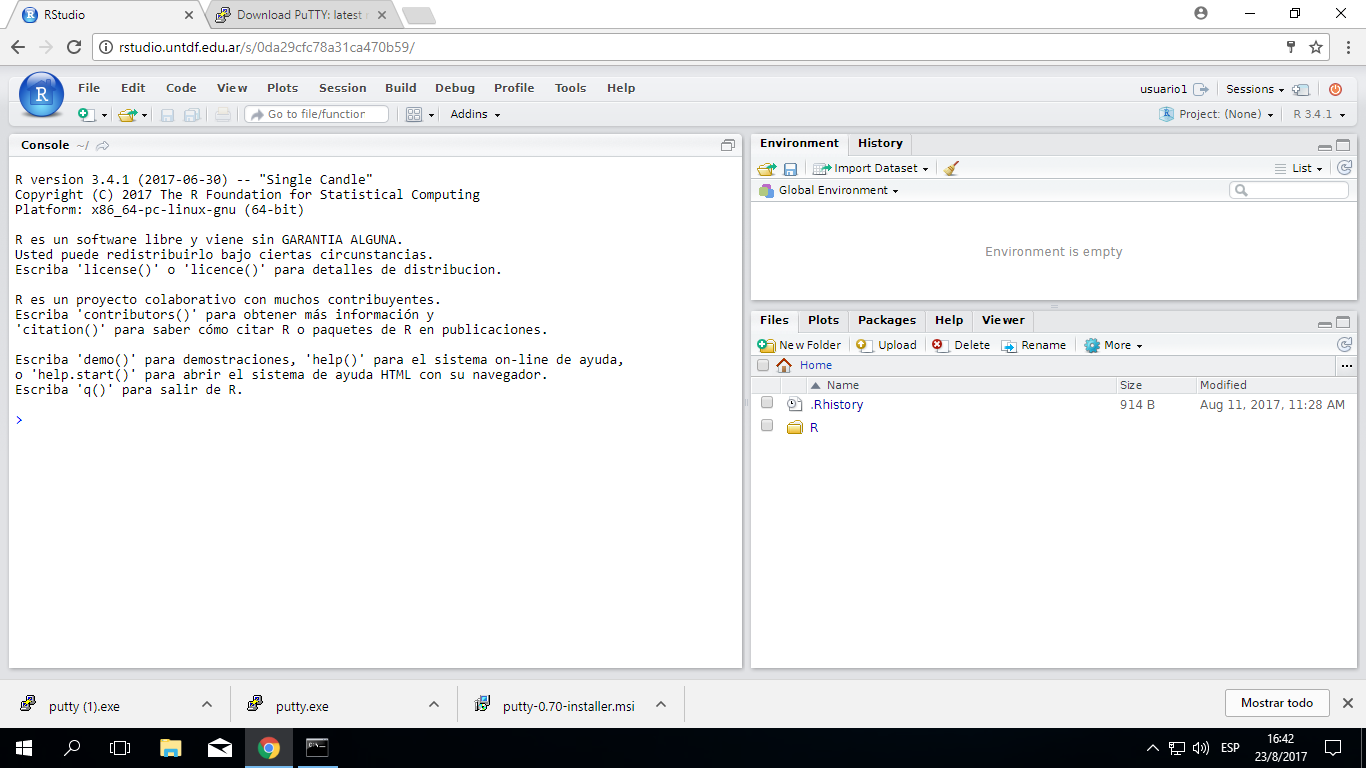
\includegraphics{fig/rstudio.png}

\hypertarget{rstudio}{%
\section{RStudio}\label{rstudio}}

La interfaz de RStudio está dividida en varios paneles, y cada uno tiene
varias pestañas. Arriba a la derecha está el \emph{espacio de trabajo}
(\emph{Environment}), es donde van a aparecer los objetos que creen a
medida que trabajan en R. La otra pestaña es el \emph{historial}
(\emph{History} ), donde quedan guardados todos los comandos que hayan
ejecutado. Abajo de estos dos hay un panel con varias pestañas.
\emph{Archivos} (\emph{Files}), muestra los archivos. \emph{Gráficos}
(\emph{Plots}) es donde van a aparecer los gráficos que vayamos
haciendo. \emph{Paquetes} (\emph{Packages}) muestra las librerías que
tenemos y sus paquetes instalados y con un tilde los cargados (más
adelante vamos a ver que son los paquetes). La \emph{ayuda}
(\emph{Help}) es donde vamos a poder la ayuda de funciones de
\textbf{R}. Y además está las pestaña del \emph{Visor} (\emph{Viewer})
que nos muestra una vista de los documentos que creemos.

Por el lado izquierdo está la \emph{consola}, es donde pasa toda la
acción. Todo lo que hagamos va a ser escrito como un orden o comando ahí
y luego vamos a ver el resultado ahí o si es un gráfico en el panel de
gráficos. Cada vez que iniciemos RStudio va a mostrar la consola con un
mensaje que indica la versión de \emph{R} y otros detalles. Debajo de
ese mensaje está el \emph{prompt}. Aquí es donde \emph{R} espera que se
ingresen los comandos. Y para interactuar con \emph{R} hay que decirle
que tiene que hacer. Los comandos y su sintaxis han evolucionado a lo
largo de décadas y ahora proveen a los usuarios una manera natural de
acceder y procesar datos, aplicar procedimientos estadísticos, etc.

Se puede usar \emph{R} como una calculadora. Podemos poner una cuenta a
realizar en el prompt y \emph{R} nos devolverá el resultado. Por
ejemplo, podemos poner:

\begin{Shaded}
\begin{Highlighting}[]
\DecValTok{2} \OperatorTok{+}\StringTok{ }\DecValTok{2}
\end{Highlighting}
\end{Shaded}

\begin{verbatim}
## [1] 4
\end{verbatim}

Prueben escribirlo en su consola justo después del ``\textgreater{}''.

También es posible guardar los resultados en un objeto:

\begin{Shaded}
\begin{Highlighting}[]
\NormalTok{x <-}\StringTok{ }\DecValTok{2} \OperatorTok{+}\StringTok{ }\DecValTok{2}
\end{Highlighting}
\end{Shaded}

Prueben hacerlo en su consola. En este caso, parece que no pasó nada. No
apareció el resultado. Pero si observan en panel del espacio de trabajo
verán que hay un nuevo objeto llamado \texttt{x}.

Prueben que sucede si escriben \texttt{x} en la consola.

\hypertarget{analisis-reproducible}{%
\section{Análisis Reproducible}\label{analisis-reproducible}}

Una ventaja que tiene \emph{R} respecto a otros programas estadísticos
es que permite reproducir el análisis de los datos. Reproducible
significa que a partir de los mismos datos otro analista va a llegar a
los mismos resultados. En cambio, replicable es que otro experimentador
al repetir el experimento va a llegar a resultados diferentes, que
pueden ser o no similares (Figura \ref{fig:reproducible-figura})

\begin{figure}

{\centering 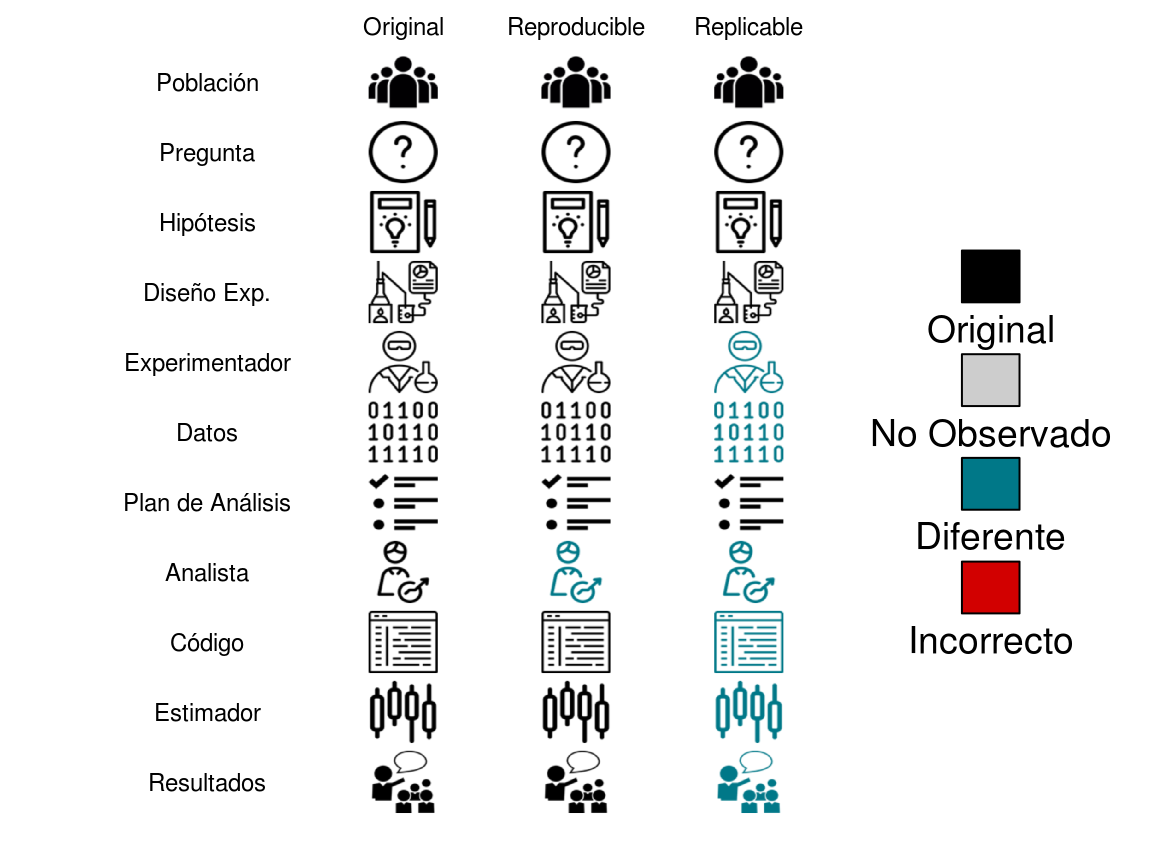
\includegraphics{Introduccion_files/figure-latex/reproducible-figura-1} 

}

\caption{Diferencias entre reproducible y replicable.}\label{fig:reproducible-figura}
\end{figure}

Los programas de interfaz gráfica, que no usan código o no lo proveen,
complican la reproducibilidad de los análisis. Esto se debe a que es más
complicado de comunicar como se realizó el análisis. La ventaja del
código es que queda todo explícito en él.

Hay varias formas de trabajar con R. Una es de forma interactiva en la
consola. Como cuando pusieron \texttt{2\ +\ 2}. Esto es muy útil cuando
estamos probando si algo funciona. Pero no guardamos el código de esta
forma. Aunque, en verdad queda guardado en el orden en que lo ejecutamos
en el historial no es útil porque se va sobreescribiendo y va quedando
lo que funcionó y lo no que no. Otra forma de usar \emph{R} es
utilizando \emph{scripts} (archivos con extensión \emph{.R}). Es
indispensable para crear nuevas funciones pero para analizar datos tiene
sus desventajas. Ya que, si bien el código se puede comentar
anteponiendo \emph{\#} a la línea que queremos comentar, es límitado el
formato que podemos usar en el comentario. Además, tendremos que volver
a correr el script para ver los resultados si no los guardamos
explicitamente en un documento, hoja de cálculo, o imagen. Por último,
tenemos los documentos de programación letrada. La programación letrada
consiste en mezclar código con texto plano, como en un procesador de
texto.

En R, hay varias aproximaciones a esto. La que más éxito ha tenido es
\emph{knitr}. \emph{To knit} es tejer en inglés, lo que hace es
``tejer'' el documento final con el resultado del código, es decir los
análisis que hagamos, y texto explicando que hicimos, porque, y como. Es
decir, podemos escribir un paper o informe completo. Para darle formato
al texto se usa \emph{markdown} que permite usar marcas livianas para
poner \emph{cursivas}, \textbf{negritas} o \sout{tachado}.

\hypertarget{rmarkdown}{%
\subsection{Rmarkdown}\label{rmarkdown}}

Hay muchas opciones para formatear el texto. La idea detrás de markdown
es que se pueda escribir en un procesador de texto sencillo y las marcas
sean fáciles de poner y no interrumpan la lectura. Algunos ejemplos:

\hypertarget{enfasis}{%
\subsubsection{Énfasis}\label{enfasis}}

\begin{verbatim}
*cursiva*   **negrita**

_cursiva_   __negrita__
\end{verbatim}

\hypertarget{titulos}{%
\subsubsection{Títulos}\label{titulos}}

\begin{verbatim}
# Título 1

## Título 2

### Título 3
\end{verbatim}

\hypertarget{listas}{%
\subsubsection{Listas}\label{listas}}

\begin{verbatim}
Lista Desordenada
* Item 1
* Item 2
    + Item 2a
    + Item 2b
Lista Ordenada
1. Item 1
2. Item 2
3. Item 3
    + Item 3a
    + Item 3b
\end{verbatim}

\hypertarget{saltos-de-linea-manuales}{%
\subsubsection{Saltos de línea
manuales}\label{saltos-de-linea-manuales}}

Termina una línea con dos o más espacios:

Las rosas son rojas,\\
las violetas son azules.

\hypertarget{vinculos}{%
\subsubsection{Vínculos}\label{vinculos}}

Usa una dirección http simple o agrega un vínculo a una frase:

\begin{verbatim}
http://example.com

[frase vínculada](http://example.com)
\end{verbatim}

\hypertarget{imagenes}{%
\subsubsection{Imágenes}\label{imagenes}}

Imágenes en la web o en el mismo directorio de trabajo:

\begin{verbatim}
![alt text](http://example.com/logo.png)

![alt text](figures/img.png)
\end{verbatim}

\BeginKnitrBlock{exercise}[Probando markdown]
\protect\hypertarget{exr:ejercicio-1}{}{\label{exr:ejercicio-1}
\iffalse (Probando markdown) \fi{} }Descarguen un archivo de RMarkdown
usando este código en la consola:

\texttt{download.file("url",\ "ejercicio-1.Rmd")}

Una vez descargado, abranlo desde el panel \emph{Files}.
\EndKnitrBlock{exercise}

Los prácticos en general se harán en un archivo similar a este. En la
parte superior encontran el encabezado entre guiones. Ahí deberán poner
sus nombres y el nombre del grupo.

\BeginKnitrBlock{exercise}[Personalizando]
\protect\hypertarget{exr:ejercicio-2}{}{\label{exr:ejercicio-2}
\iffalse (Personalizando) \fi{} }Cambien en encabezado y pongan sus
nombres, el nombre del grupo y la fecha de hoy.
\EndKnitrBlock{exercise}

Abajo encontraran espacio para ir contestando la preguntas. Una
consideración que deben tomar en cuenta es que todo el texto que
escriban va a ser considerado como un \emph{único} párrafo a menos que
este separado por \textbf{una línea en blanco}.

Por ejemplo, prueben escribir esto en el documento (pueden copiarlo):

\begin{quote}
Mucho antes de que el lector haya llegado a esta parte de mi obra se le
habrán ocurrido una multitud de dificultades. Algunas son tan graves,
que aun hoy dia apenas puedo reflexionar sobre ellas sin vacilar algo;
pero, según mi leal saber y entender, la mayor parte son solo aparentes,
y las que son reales no son, creo yo, funestas para mi teoria.
\end{quote}

\begin{quote}
Estas dificultades y objeciones pueden clasificarse en los siguientes
grupos:
\end{quote}

\begin{quote}
1° Si las especies han descendido de otras especies por suaves
gradaciones, ¿por qué no encontramos en todas partes innumerables formas
de transicion? ¿Por qué no está toda la naturaleza confusa, en lugar de
estar las especies bien definidas según las vemos?

2° ¿Es posible que un animal que tiene, por ejemplo, la conformación y
costumbres de un murciélago pueda haber sido formado por modificación de
otro animal de costumbres y estructura muy diferentes? ¿Podemos creer
que la selecci6n natural pueda producir, de una parte, un órgano
insignificante, tal como la cola de la jirafa, que sirve de mosqueador,
y, de otra, un órgano tan maravilloso como el ojo?

3° ¿Pueden los instintos adquirirse y modificarse por selección natural?
¿Qué diremos del instinto que lleva a la abeja a hacer celdas y que
prácticamente se ha anticipado a los descubrimientos de profundos
matemáticos?

4° ¿Cómo podemos explicar que cuando se cruzan las especies son
esteriles o producen descendencia esteril, mientras que cuando se cruzan
las variedades su fecundidad es sin igual?
\end{quote}

Luego, hagan clic en el botón \emph{Knit} que tienen arriba, al lado de
un ovillo y una aguja de tejer. El desafío es mantener el formato con
cada párrafo separado.

La misma consideración se debe tener en cuenta para otros formatos como
títulos o listas. Un consejo para ver como va quedando el documento, es
tejerlo seguido. Así podremos ver cualquier problema pronto.

\hypertarget{integrando-codigo}{%
\section{Integrando código}\label{integrando-codigo}}

En los documentos de RMarkdown se puede integrar bloques de código (de
\emph{R} y otros lenguajes). Para insertar un bloque pueden hacer clic
en el botón de ``Insert/R'' que hay arriba o por el atajo del teclado
``Ctrl+Alt+I''.

\begin{verbatim}
```{r}
\end{verbatim}

\begin{Shaded}
\begin{Highlighting}[]
\NormalTok{Acá va el código}
\end{Highlighting}
\end{Shaded}

\begin{verbatim}
```
\end{verbatim}

Es importante mantener las comillas invertidas tal cual están ya que con
ellas se define donde empieza y termina el bloque. Entre las llaves se
incluye como se va a ejecutar el código (con \emph{R} en este caso).
También se puede poner nombre al bloque, cosa que es muy recomendable
porque sino van a estar nombrados como chunk-\#, donde \# son números
consecutivos. Ahora, imaginen que el chunk-34 de 60 falla. Va a ser un
poco tedioso buscarlo, con nombre será más sencillo saber donde estar el
fallo. Además se pueden poner otras opciones, como ocultar el código,
cambiar el tamaño de figuras, etc. Luego de las llaves, en \emph{la
línea siguiente}, deben introducir el código que quieran ejecutar,
siempre teniendo en cuenta de dejar la línea con las comillas invertidas
tal cual está. También es buena idea dejar una línea en blanco luego.

\BeginKnitrBlock{exercise}
\protect\hypertarget{exr:ejercicio-3}{}{\label{exr:ejercicio-3} }Incluyan un
bloque de código y pongan un nombre descriptivo. Luego, escriban una
operación matemática simple. Finalmente, tejan el documento.
\EndKnitrBlock{exercise}

\hypertarget{visualizacion-de-datos}{%
\chapter{Visualización de Datos}\label{visualizacion-de-datos}}

\begin{atencion}
Para hacer el tutorial ingresen este código en la consola:

\texttt{download.file("git.io/visualizacion.Rmd",\ file\ =\ "visualizacion.Rmd")}

A continuación abran el archivo \texttt{visualizacion.Rmd} y hagan clic
en el botón \texttt{Run\ document} arriba.
\end{atencion}

\hypertarget{introduccion}{%
\section{Introducción}\label{introduccion}}

Una de las formas más útiles de visualizar la información es mediante
gráficos (aunque si son pocos datos es preferible una tabla). De hecho,
el primer paso antes de analizar los datos debe ser hacer un gráfico de
los valores que tienen. Un gráfico de dispersión si es bidimensional o
un histograma si solo tiene una dimensión.

Aunque hay varios sistemas gráficos (\texttt{base}, \texttt{lattice},
\texttt{ggobi}, \texttt{plotly}) vamos a usar \texttt{ggplot2} por su
facilidad de uso y potencia para hacer gráficos complejos a partir de
componentes simples.

Este paquete sigue una idea que se llama gramática de gráficos propuesta
por Wilkinson en donde los gráficos pueden dividirse en cuatro partes:

\begin{itemize}
\tightlist
\item
  Los \textbf{datos} y como se \textbf{mapea} (\textbf{\texttt{aes}})
  esos datos a las diferentes atributos estéticos. Es decir que columna
  corresponde al eje x, al eje y, forma, color, etc.
\item
  Las formas geométricas (\textbf{\texttt{geom}}) que representan como
  se ven los datos. Como puntos, líneas, barras de error, etc.
\item
  Transformaciones estadísticas de los datos (\textbf{\texttt{stats}})
  resumen los datos de forma útil. Por ejemplo, para agregar la media
  por grupo o una línea de regresión sin haberlos calculado antes.
\item
  Escalas a las que se mapean los datos (\textbf{\texttt{scale}}). Estas
  pueden ser escalas de color, forma, etc.
\item
  Un sistema de coordenadas (\textbf{\texttt{coord}}), que describe como
  se proyectan estos datos. Por defecto se usa el sistema cartesiano.
  Pero hay otros disponibles como el polar.
\item
  Un sistema paneles (\textbf{\texttt{facet}}) que describe como dividir
  los datos en distintos paneles.
\end{itemize}

Adicionalmente a la gramática, se agrega un sistema de temas que permite
modificar la totalidad de elementos que hacen al gráfico como fuentes,
líneas de ejes, etc.

\hypertarget{el-conjunto-de-datos-mpg}{%
\section{\texorpdfstring{El conjunto de datos
\texttt{mpg}}{El conjunto de datos mpg}}\label{el-conjunto-de-datos-mpg}}

En los datos que vienen con el paquete \texttt{ggplot2} está
\texttt{mpg}. Contiene los datos de rendimiento, cilindrada y otros más
de algunos modelos de autos. Los datos están una estructura rectangular
llamada \emph{data frame}, cada columna es una variable y cada fila una
observación recolectadas por la Agencia de Protección ambiental de
EE.UU.

\begin{Shaded}
\begin{Highlighting}[]
\KeywordTok{library}\NormalTok{(tidyverse)}
\NormalTok{mpg}
\end{Highlighting}
\end{Shaded}

\begin{verbatim}
## # A tibble: 234 x 11
##    manufacturer model    displ  year   cyl trans   drv     cty   hwy fl   
##    <chr>        <chr>    <dbl> <int> <int> <chr>   <chr> <int> <int> <chr>
##  1 audi         a4        1.80  1999     4 auto(l~ f        18    29 p    
##  2 audi         a4        1.80  1999     4 manual~ f        21    29 p    
##  3 audi         a4        2.00  2008     4 manual~ f        20    31 p    
##  4 audi         a4        2.00  2008     4 auto(a~ f        21    30 p    
##  5 audi         a4        2.80  1999     6 auto(l~ f        16    26 p    
##  6 audi         a4        2.80  1999     6 manual~ f        18    26 p    
##  7 audi         a4        3.10  2008     6 auto(a~ f        18    27 p    
##  8 audi         a4 quat~  1.80  1999     4 manual~ 4        18    26 p    
##  9 audi         a4 quat~  1.80  1999     4 auto(l~ 4        16    25 p    
## 10 audi         a4 quat~  2.00  2008     4 manual~ 4        20    28 p    
## # ... with 224 more rows, and 1 more variable: class <chr>
\end{verbatim}

\hypertarget{graficos-con-ggplot}{%
\section{Gráficos con ggplot}\label{graficos-con-ggplot}}

Podemos hacer un gráfico de la siguiente forma:

\begin{Shaded}
\begin{Highlighting}[]
\KeywordTok{library}\NormalTok{(ggplot2)}
\KeywordTok{ggplot}\NormalTok{(}\DataTypeTok{data =}\NormalTok{ mpg) }\OperatorTok{+}
\StringTok{ }\KeywordTok{geom_point}\NormalTok{(}\DataTypeTok{mapping =} \KeywordTok{aes}\NormalTok{(}\DataTypeTok{x =}\NormalTok{ displ, }\DataTypeTok{y =}\NormalTok{ hwy))}
\end{Highlighting}
\end{Shaded}

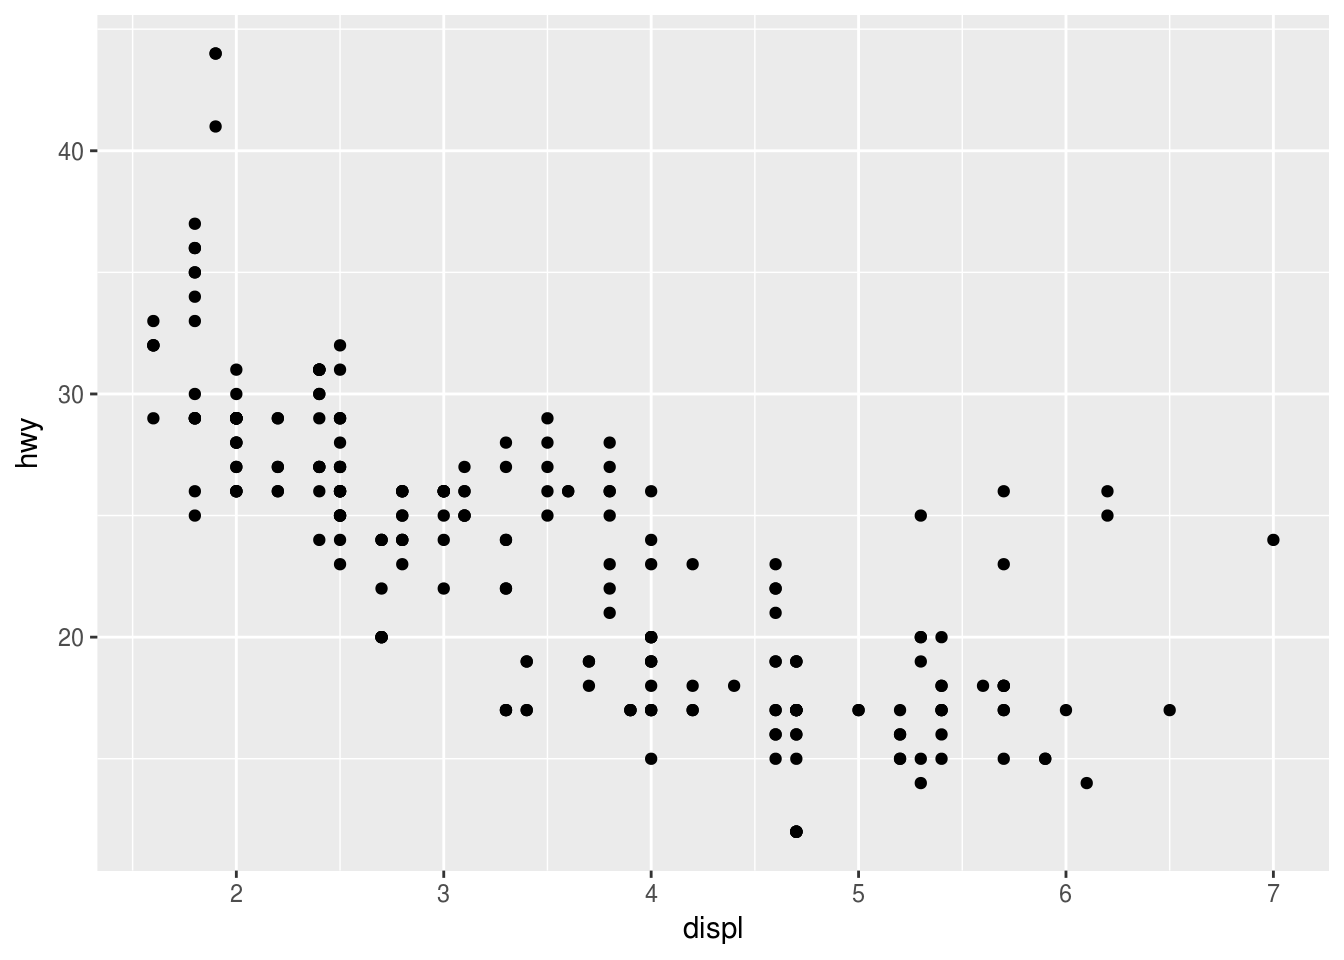
\includegraphics{Graficos_files/figure-latex/grafico-inicial-1.pdf}

Prueben escribiendo el código en la consola.

En el gráfico vemos que hay una tendencia a disminuir el rendimiento a
medida que aumenta la cilindrada.

En la llamada de Hay distintas partes. La llamada a \texttt{ggplot}
donde especificamos el nombre de los datos que vamos a usar. Es la que
inicializa el gráfico. Pero aquí no especifica nada de como graficarlo.
Sin embargo, es necesario empezar siempre por esta función y luego ir
agregando capas. Luego agregamos una capa de puntos. Ambos están unidos
por un \texttt{+}. Cada vez que deseemos agregar una capa, lo haremos
con ese símbolo \texttt{+}. Por otro lado, especificamos el mapeo de las
columnas de los datos a las ordenadas y abscisas dentro del argumento
\texttt{mapping}. Hemos graficado el tamaño del motor (en litros),
\texttt{displ} en las ordenadas y el rendimiento en millas por galón en
las abscisas. Siempre que quereamos mapear una columna a alguna parte
del gráfico lo hemos de hacer dentro la función \texttt{aes()}, de
\emph{aestetics} que significa ésteticas en inglés.

\hypertarget{mapeando}{%
\section{Mapeando}\label{mapeando}}

En el gráfico anterior vemos que hay unos puntos que no siguen la
tendencia general. Aquí están resaltados con rojo.

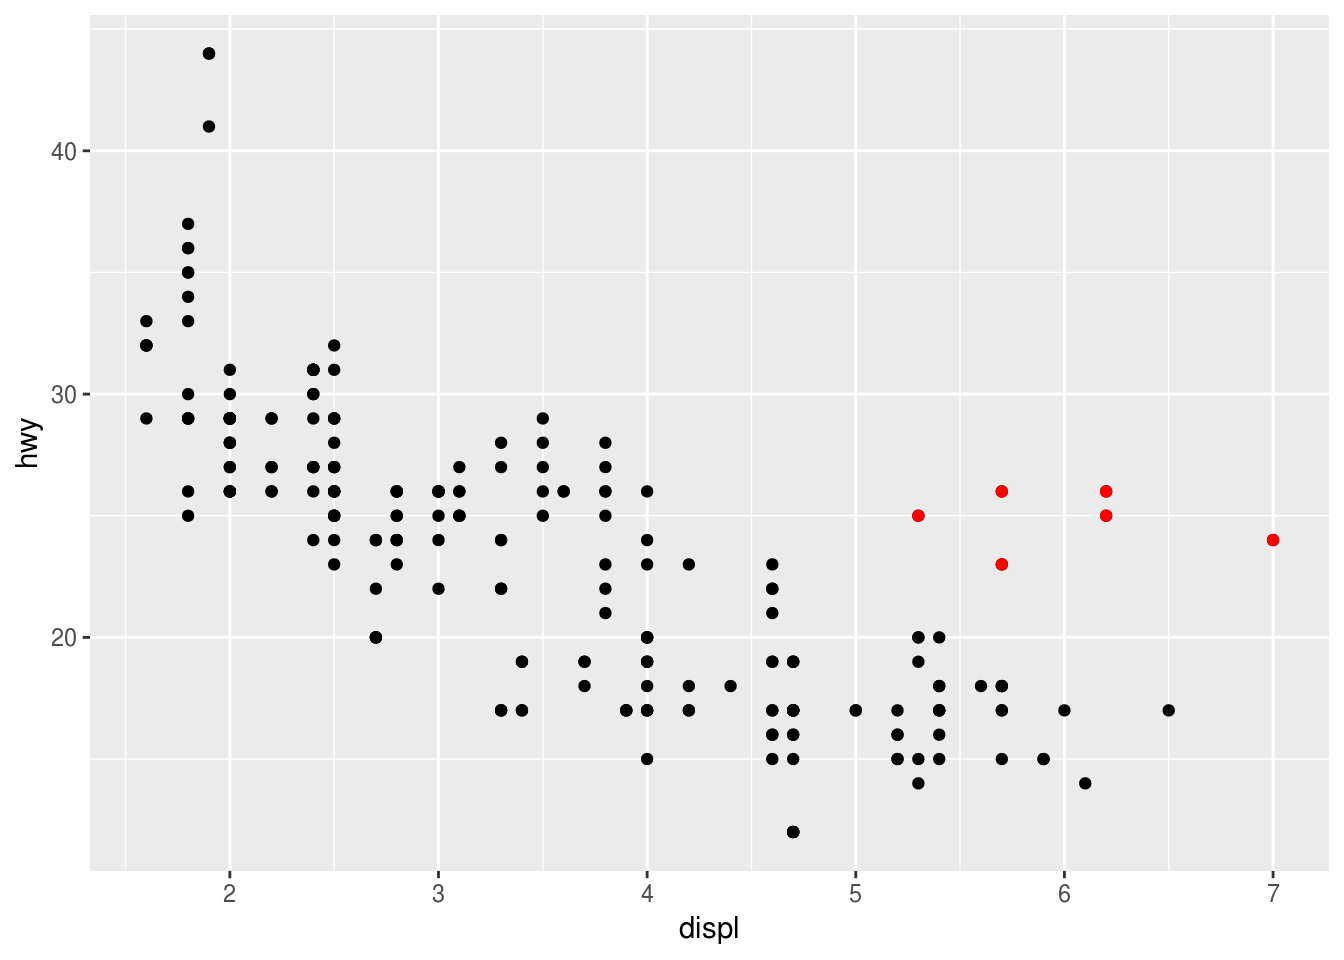
\includegraphics{Graficos_files/figure-latex/puntos-resaltados-1.pdf}

Para saber más el porque de estos puntos podríamos agregar más
información al gráfico como por ejemplo el tipo de auto. Una opción es
agregar colores.

\begin{Shaded}
\begin{Highlighting}[]
\KeywordTok{ggplot}\NormalTok{(}\DataTypeTok{data =}\NormalTok{ mpg) }\OperatorTok{+}
\StringTok{ }\KeywordTok{geom_point}\NormalTok{(}\DataTypeTok{mapping =} \KeywordTok{aes}\NormalTok{(}\DataTypeTok{x =}\NormalTok{ displ, }\DataTypeTok{y =}\NormalTok{ hwy, }\DataTypeTok{color =}\NormalTok{ class))}
\end{Highlighting}
\end{Shaded}

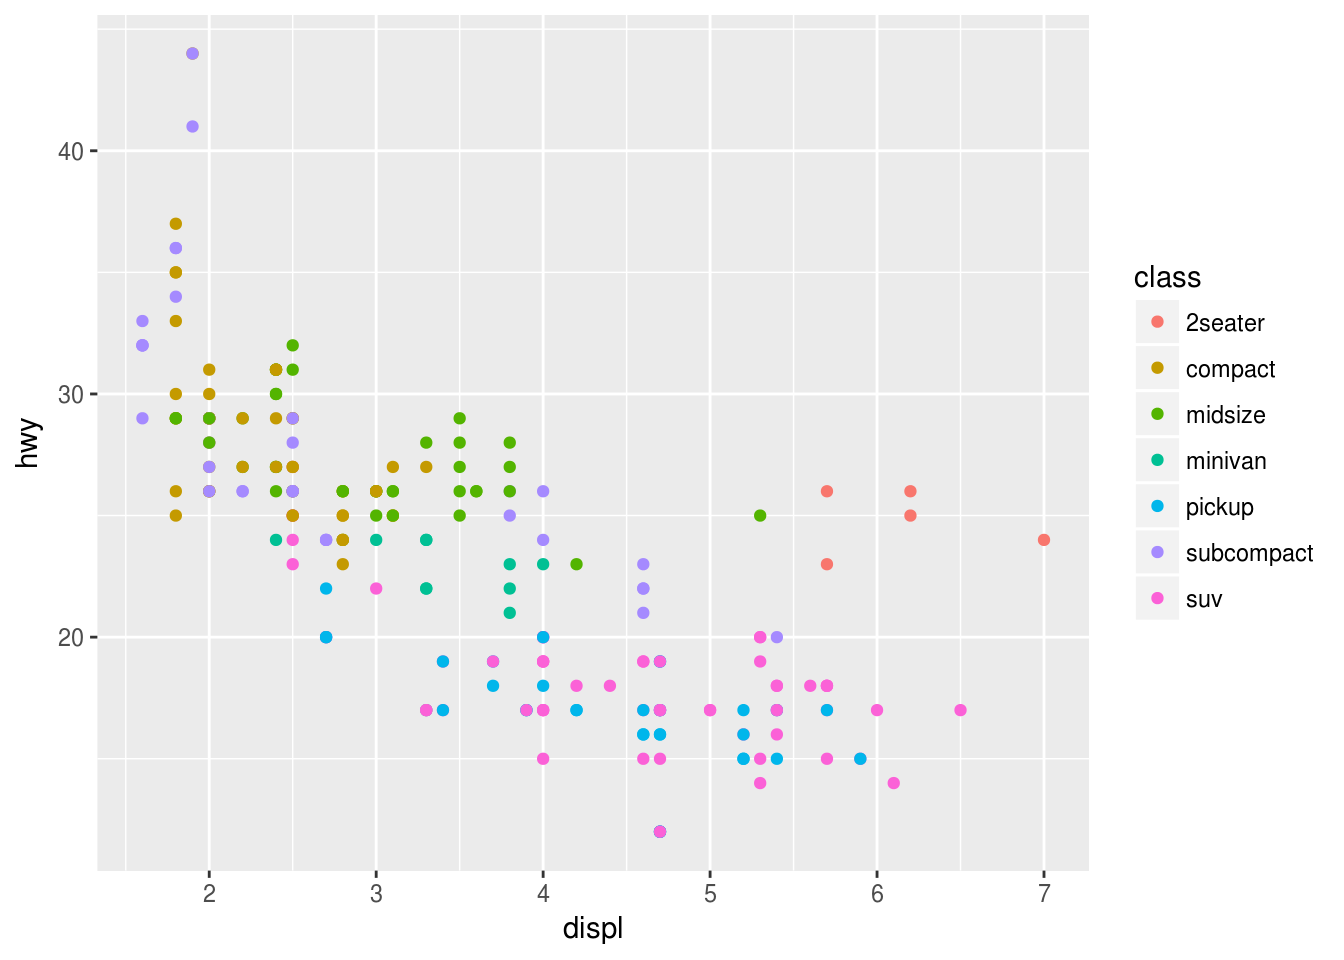
\includegraphics{Graficos_files/figure-latex/color-1.pdf}

Ahora podemos ver, que en general los autos con cilindrada grande son
camionetas (\emph{pickup}) o suv. Y que los que tienen cilindrada grande
pero rendimiento mayor son autos deportivos.

Agregamos el color mapeando \texttt{class} a la éstetica de color.
\texttt{ggplot} le asigna automáticamente un color a cada nivel de
\texttt{class}. Y también genera la leyenda apropiada.

También podemos mapear el tamaño del punto a \texttt{class}. En este
caso recibiremos un \texttt{warning} porque no tiene mucho sentido
mapear el tamaño con una variable discreta desordenada. Es decir, que no
hay una correspondencia entre el tamaño del punto y la clase.

\begin{Shaded}
\begin{Highlighting}[]
\KeywordTok{ggplot}\NormalTok{(}\DataTypeTok{data =}\NormalTok{ mpg) }\OperatorTok{+}
\StringTok{ }\KeywordTok{geom_point}\NormalTok{(}\DataTypeTok{mapping =} \KeywordTok{aes}\NormalTok{(}\DataTypeTok{x =}\NormalTok{ displ, }\DataTypeTok{y =}\NormalTok{ hwy, }\DataTypeTok{size =}\NormalTok{ class))}
\end{Highlighting}
\end{Shaded}

\begin{verbatim}
## Warning: Using size for a discrete variable is not advised.
\end{verbatim}

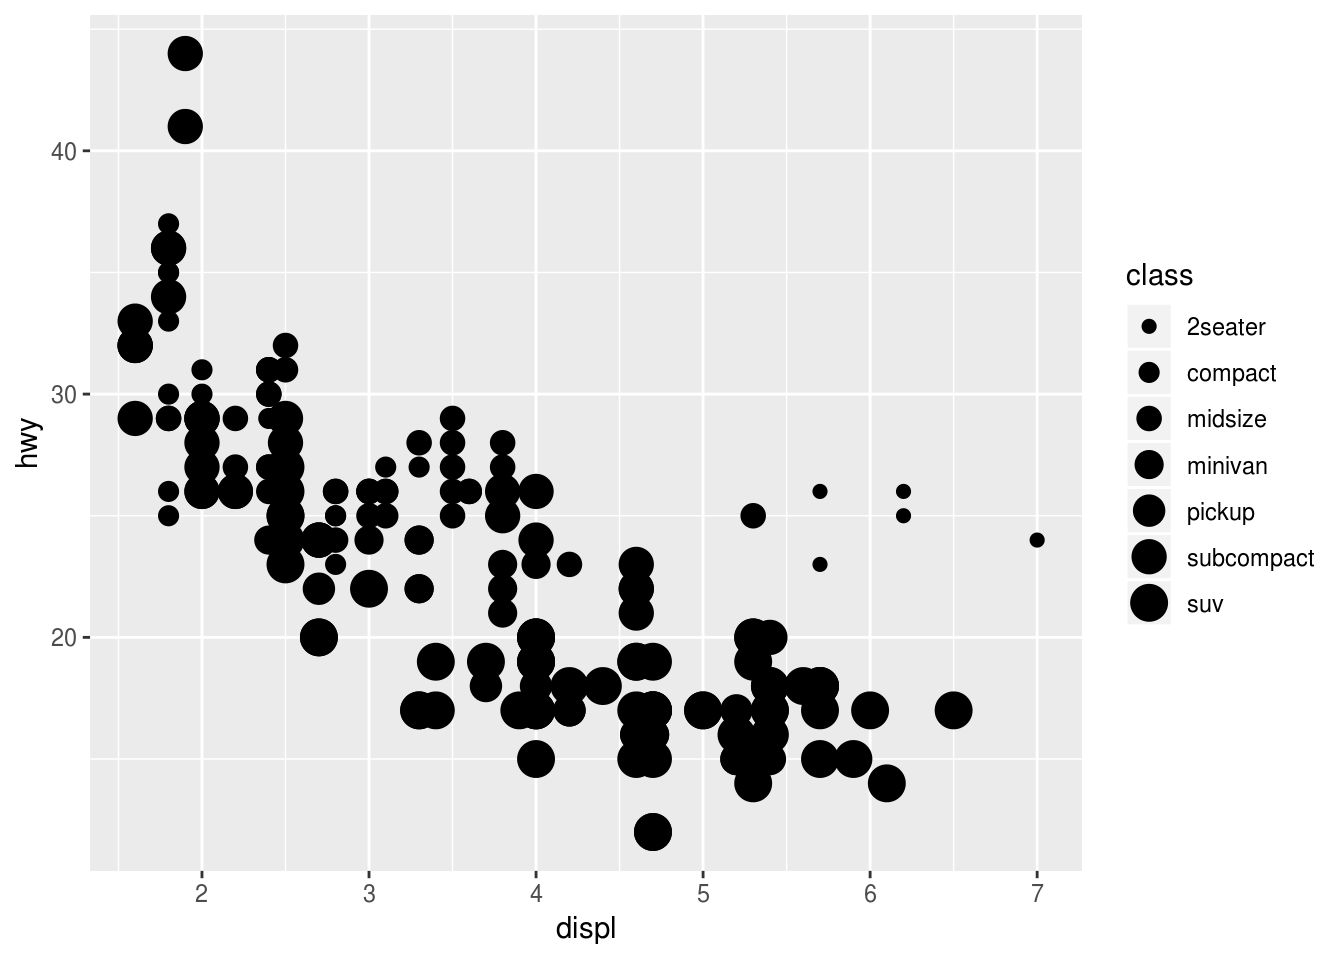
\includegraphics{Graficos_files/figure-latex/point-size-1.pdf}

También podriamos mapear la clase a la transparencia de los puntos
(\texttt{alpha}) o a la forma (\texttt{shape})

\begin{Shaded}
\begin{Highlighting}[]
\CommentTok{# Izquierda}
\KeywordTok{ggplot}\NormalTok{(}\DataTypeTok{data =}\NormalTok{ mpg) }\OperatorTok{+}\StringTok{ }
\StringTok{  }\KeywordTok{geom_point}\NormalTok{(}\DataTypeTok{mapping =} \KeywordTok{aes}\NormalTok{(}\DataTypeTok{x =}\NormalTok{ displ, }\DataTypeTok{y =}\NormalTok{ hwy, }\DataTypeTok{alpha =}\NormalTok{ class))}

\CommentTok{# Derecha}
\KeywordTok{ggplot}\NormalTok{(}\DataTypeTok{data =}\NormalTok{ mpg) }\OperatorTok{+}\StringTok{ }
\StringTok{  }\KeywordTok{geom_point}\NormalTok{(}\DataTypeTok{mapping =} \KeywordTok{aes}\NormalTok{(}\DataTypeTok{x =}\NormalTok{ displ, }\DataTypeTok{y =}\NormalTok{ hwy, }\DataTypeTok{shape =}\NormalTok{ class))}
\end{Highlighting}
\end{Shaded}

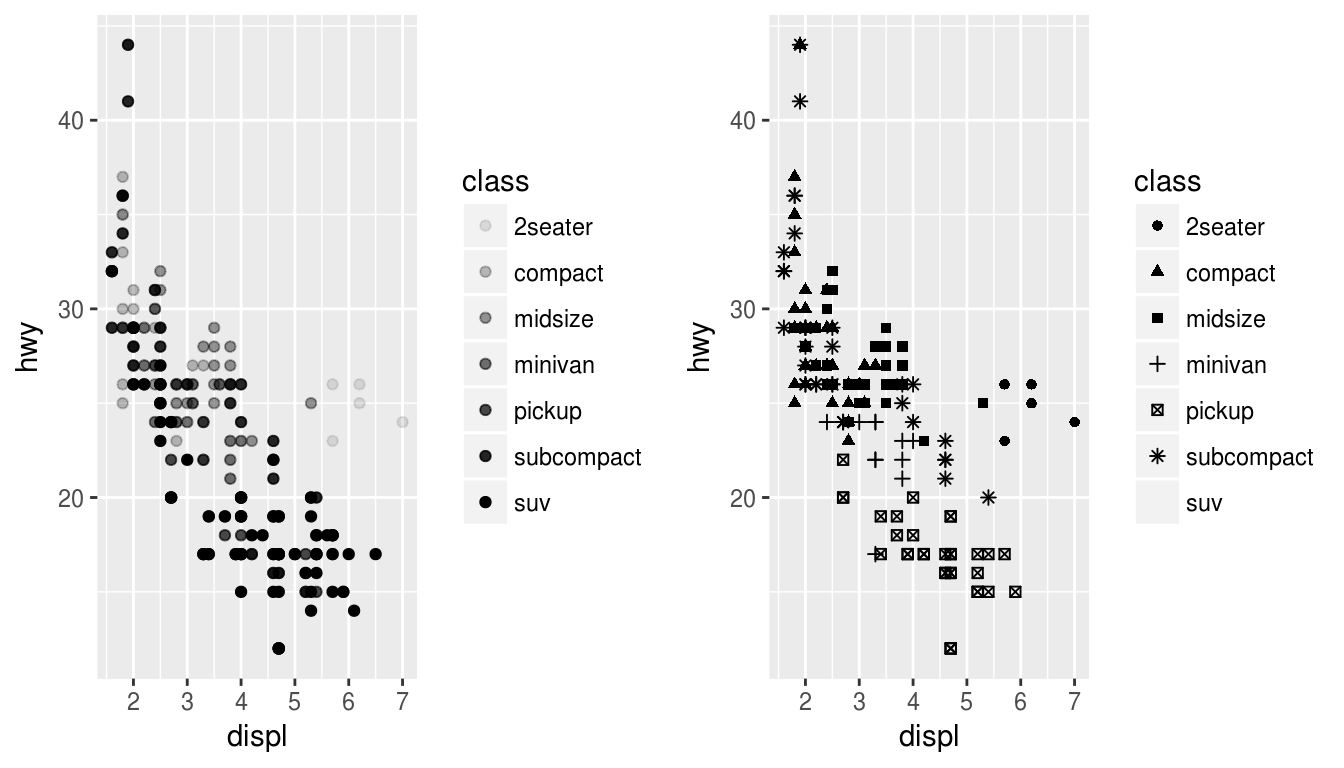
\includegraphics{Graficos_files/figure-latex/alpha-shape-1.pdf}

Si reproducen el código en sus computadoras verán que que ambos dan
advertencias. Así como no tienen mucho sentido mapear el tamaño a algo
sin orden intríseco, tampoco lo tiene mapear la transparencia. Por otro
lado, noten que en el gráfico de la derecha ¡faltan los puntos de
\emph{suv}! Esto es porque ggplot solo asigna automaticamente hasta 6
símbolos diferentes para los puntos. Si queremos más hay que hacerlo de
forma manual.

En general, uno mapea una variable a alguna característica del gráfico
asociandola dentro de \texttt{aes()}. \texttt{ggplot} se encarga de los
detalles de pasar esa asociación a las distintas capas, de generar los
niveles apropiados y de hacer la leyenda. De hecho, podemos ver que
\emph{x} e \emph{y} también son características del gráfico pero en vez
de mostrar una leyenda genera las marcas en los ejes.

También es posible configurar alguna estética a un valor específico.
Como por ejemplo hacer que todos los puntos sean rojos

\begin{Shaded}
\begin{Highlighting}[]
\KeywordTok{ggplot}\NormalTok{(}\DataTypeTok{data =}\NormalTok{ mpg) }\OperatorTok{+}\StringTok{ }
\StringTok{  }\KeywordTok{geom_point}\NormalTok{(}\DataTypeTok{mapping =} \KeywordTok{aes}\NormalTok{(}\DataTypeTok{x =}\NormalTok{ displ, }\DataTypeTok{y =}\NormalTok{ hwy), }\DataTypeTok{color =} \StringTok{"red"}\NormalTok{)}
\end{Highlighting}
\end{Shaded}

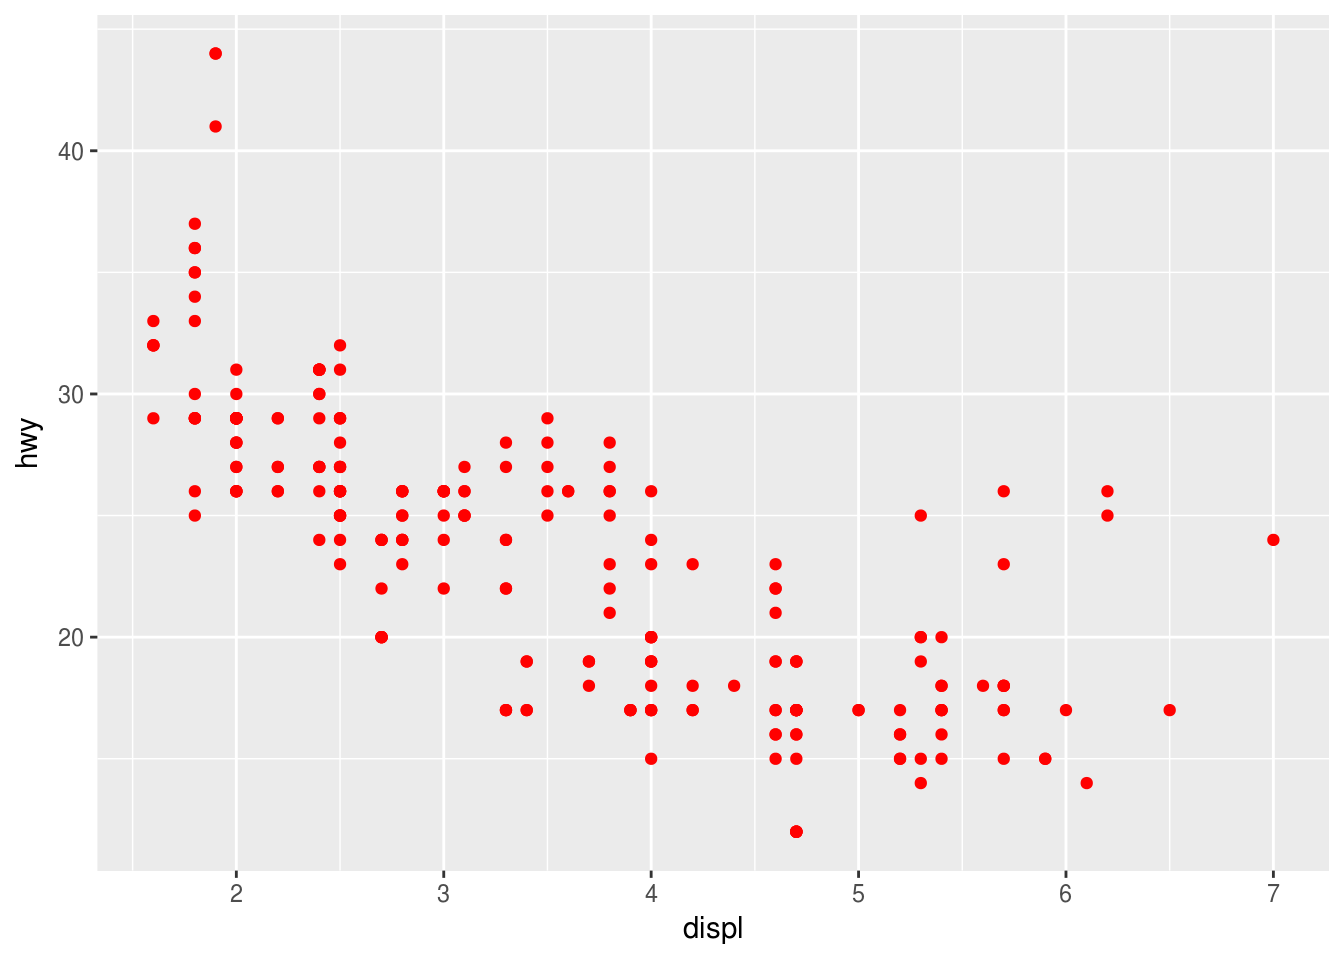
\includegraphics{Graficos_files/figure-latex/manual-color-1.pdf}

Acá el color no muestra ninguna información extra. También es posible
cambiar el:

\begin{itemize}
\tightlist
\item
  el color por el nombre que tenga sentido o en hexadecimal.
\item
  el tamaño de los puntos en mm.
\item
  la forma del punto según los valores que se muestran acá abajo
\end{itemize}

\begin{figure}
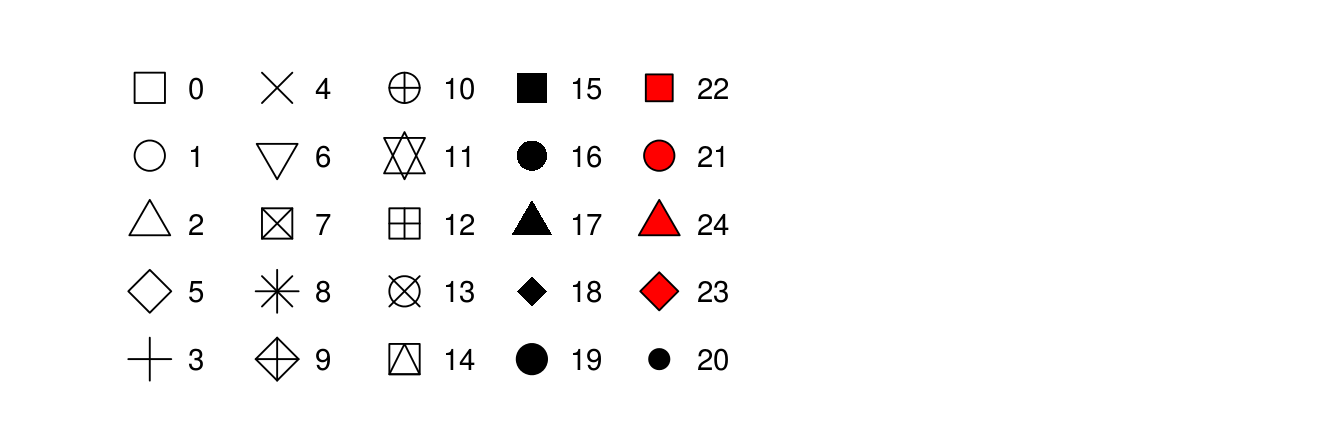
\includegraphics[width=0.75\linewidth]{Graficos_files/figure-latex/puntos-1} \caption{Valores númericos y la forma asociada a cada uno. En R hay 25 formas diferentes. Algunas parecen repetirse pero no es así. Por ejemplo, las formas 0, 15 y 22 son todos cuadrados. Pero las formas del 0-15 tienen el color definido por el borde, usan `color` para cambiar el color. Del 15 a 18 son formas rellenas que usan `fill` para cambiar el color del relleno. Y de la forma 21 a 23 son formas con relleno y borde que usan ambas `fill` y `color`.}\label{fig:puntos}
\end{figure}

Valores númericos y la forma asociada a cada uno. En R hay 25 formas
diferentes. Algunas parecen repetirse pero no es así. Por ejemplo, las
formas 0, 15 y 22 son todos cuadrados. Pero las formas del 0-15 tienen
el color definido por el borde, usan \texttt{color} para cambiar el
color. Del 15 a 18 son formas rellenas que usan \texttt{fill} para
cambiar el color del relleno. Y de la forma 21 a 23 son formas con
relleno y borde que usan ambas \texttt{fill} y \texttt{color}.

\hypertarget{formas-geometricas}{%
\section{Formas geometricas}\label{formas-geometricas}}

¿En que se parecen los gráficos de abajo?

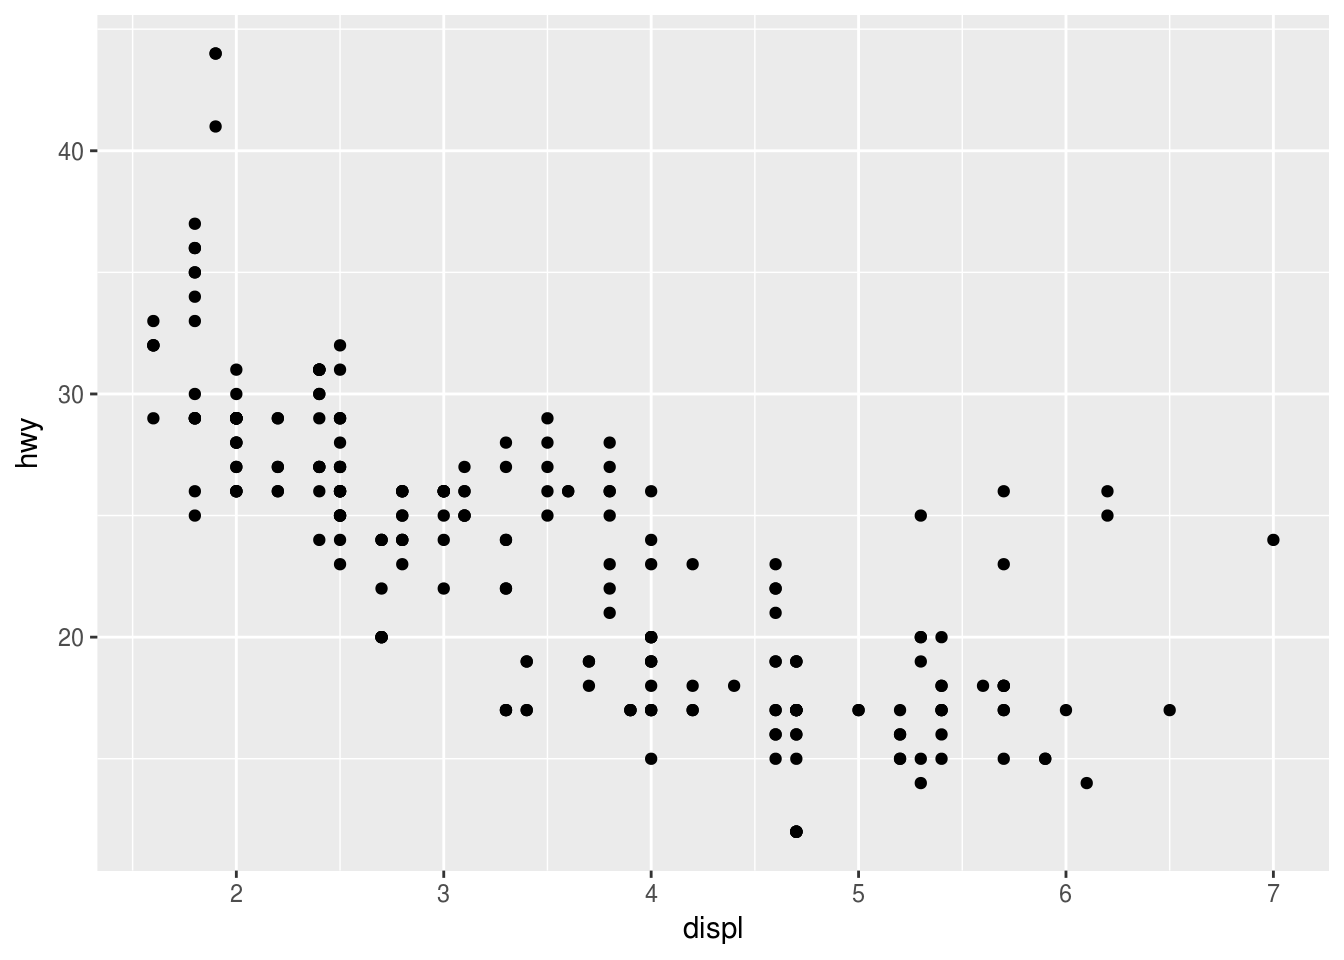
\includegraphics[width=0.5\linewidth]{Graficos_files/figure-latex/unnamed-chunk-3-1}
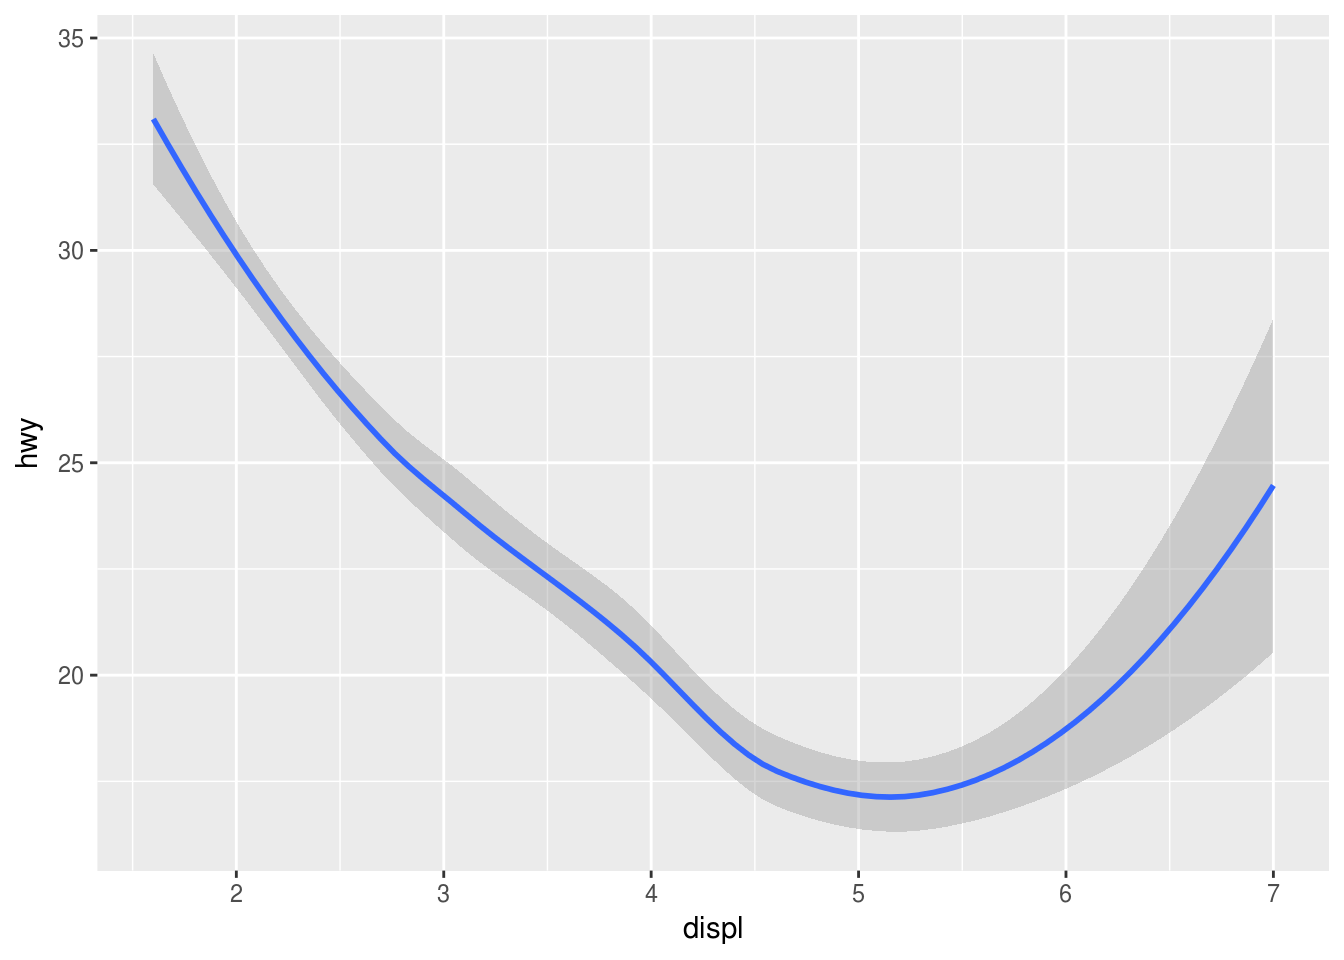
\includegraphics[width=0.5\linewidth]{Graficos_files/figure-latex/unnamed-chunk-3-2}

Ambos tienen las mismas variables, pero están representados por
distintas formas. En el idioma de ggplot cada forma es un \textbf{geom}.
Y cada geom es una forma geométrica de representar los datos. Hay muchos
\textbf{geom} (más de 30 en el paquete y muchos más en extensiones) y
todos empiezan con \textbf{\texttt{geom\_}}), por ejemplo:

\begin{table}

\caption{\label{tab:Graficos-Comunes}Gráficos comunes con ggplot}
\centering
\begin{tabular}[t]{l|l}
\hline
Gráfico & geom\\
\hline
Barras & geom\_col geom\_bar\\
\hline
Puntos & geom\_point\\
\hline
Cajas y Barras & geom\_boxplot\\
\hline
Histograma & geom\_histogram\\
\hline
Lineas & geom\_line\\
\hline
Barras de Error & geom\_errorbar\\
\hline
\end{tabular}
\end{table}

Pueden ver más en la ayuda de ggplot en R (usando la pestaña de ayuda o
usando \texttt{help(nombre\_de\_función)} en la consola) o en la
documentación online que tiene la ventaja de tener graficados los
ejemplos \url{http://ggplot2.tidyverse.org/reference/} .

Para hacer los gráficos de arriba usamos:

\begin{Shaded}
\begin{Highlighting}[]
\CommentTok{# Izquierda}
\KeywordTok{ggplot}\NormalTok{(}\DataTypeTok{data =}\NormalTok{ mpg) }\OperatorTok{+}\StringTok{ }
\StringTok{  }\KeywordTok{geom_point}\NormalTok{(}\DataTypeTok{mapping =} \KeywordTok{aes}\NormalTok{(}\DataTypeTok{x =}\NormalTok{ displ, }\DataTypeTok{y =}\NormalTok{ hwy))}

\CommentTok{# Derecha}
\KeywordTok{ggplot}\NormalTok{(}\DataTypeTok{data =}\NormalTok{ mpg) }\OperatorTok{+}\StringTok{ }
\StringTok{  }\KeywordTok{geom_smooth}\NormalTok{(}\DataTypeTok{mapping =} \KeywordTok{aes}\NormalTok{(}\DataTypeTok{x =}\NormalTok{ displ, }\DataTypeTok{y =}\NormalTok{ hwy))}
\end{Highlighting}
\end{Shaded}

Todos los \emph{geoms} van luego de \texttt{ggplot} y se unen con un
\texttt{+}. En ggplot cada forma geométrica es una capa y pueden
combinarse varias en un mismo gráfico.

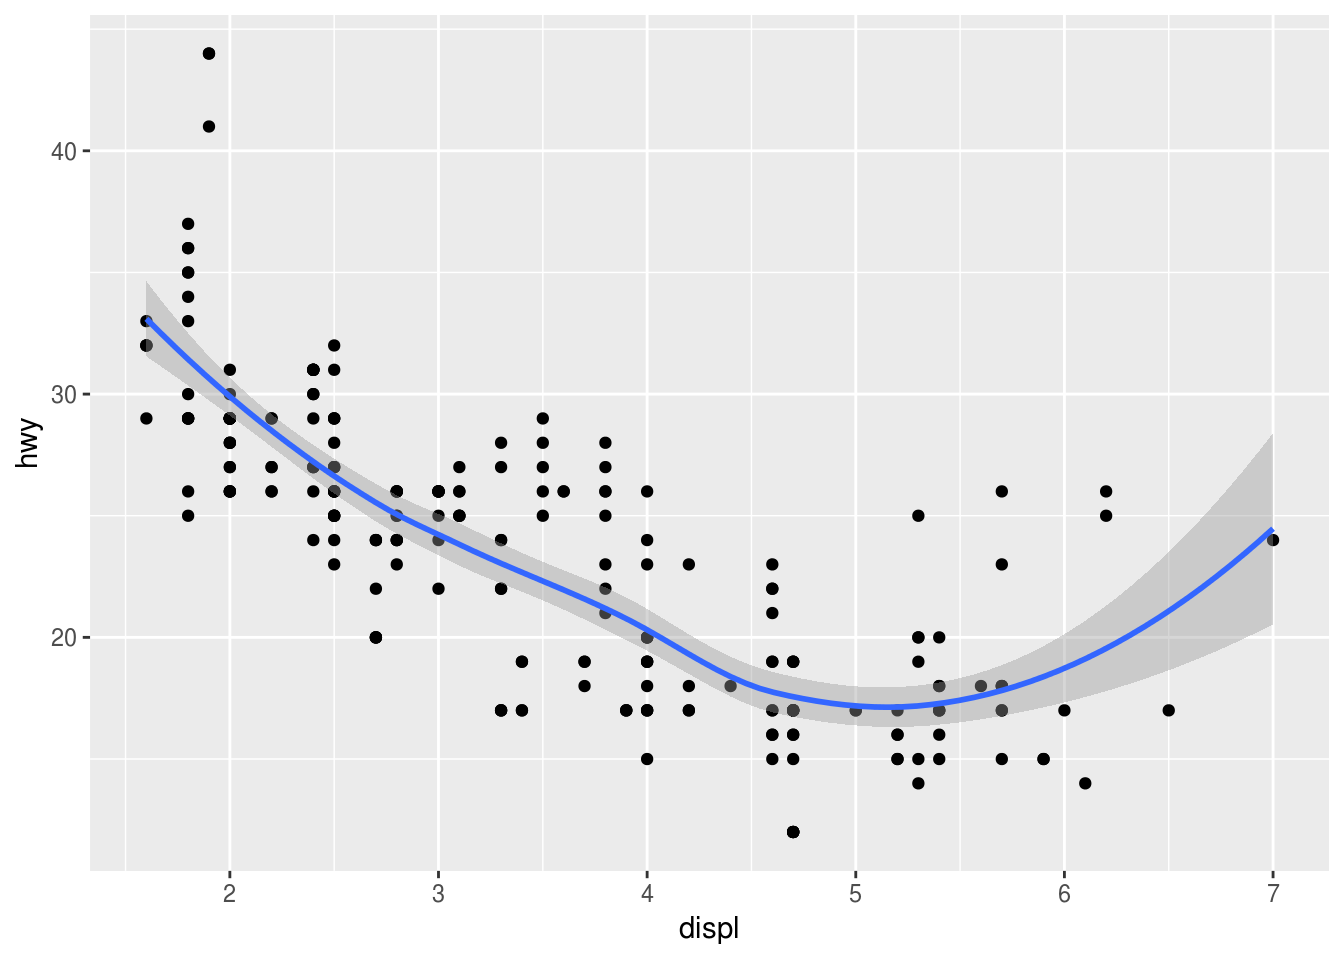
\includegraphics[width=0.5\linewidth]{Graficos_files/figure-latex/dos-geoms-1}

Además, todos los \texttt{geoms} tienen un argumento \texttt{mapping}
para la estética. Claro que no todos aceptan los mismas argumentos. No
tienen sentido ponerle relleno a una línea o cambiar el tipo de línea a
un punto. Pero si se puede cambiar el tipo de línea de `geom\_smooth:

\begin{Shaded}
\begin{Highlighting}[]
\KeywordTok{ggplot}\NormalTok{(}\DataTypeTok{data =}\NormalTok{ mpg) }\OperatorTok{+}\StringTok{ }
\StringTok{  }\KeywordTok{geom_smooth}\NormalTok{(}\DataTypeTok{mapping =} \KeywordTok{aes}\NormalTok{(}\DataTypeTok{x =}\NormalTok{ displ, }\DataTypeTok{y =}\NormalTok{ hwy, }\DataTypeTok{linetype =}\NormalTok{ drv))}
\end{Highlighting}
\end{Shaded}

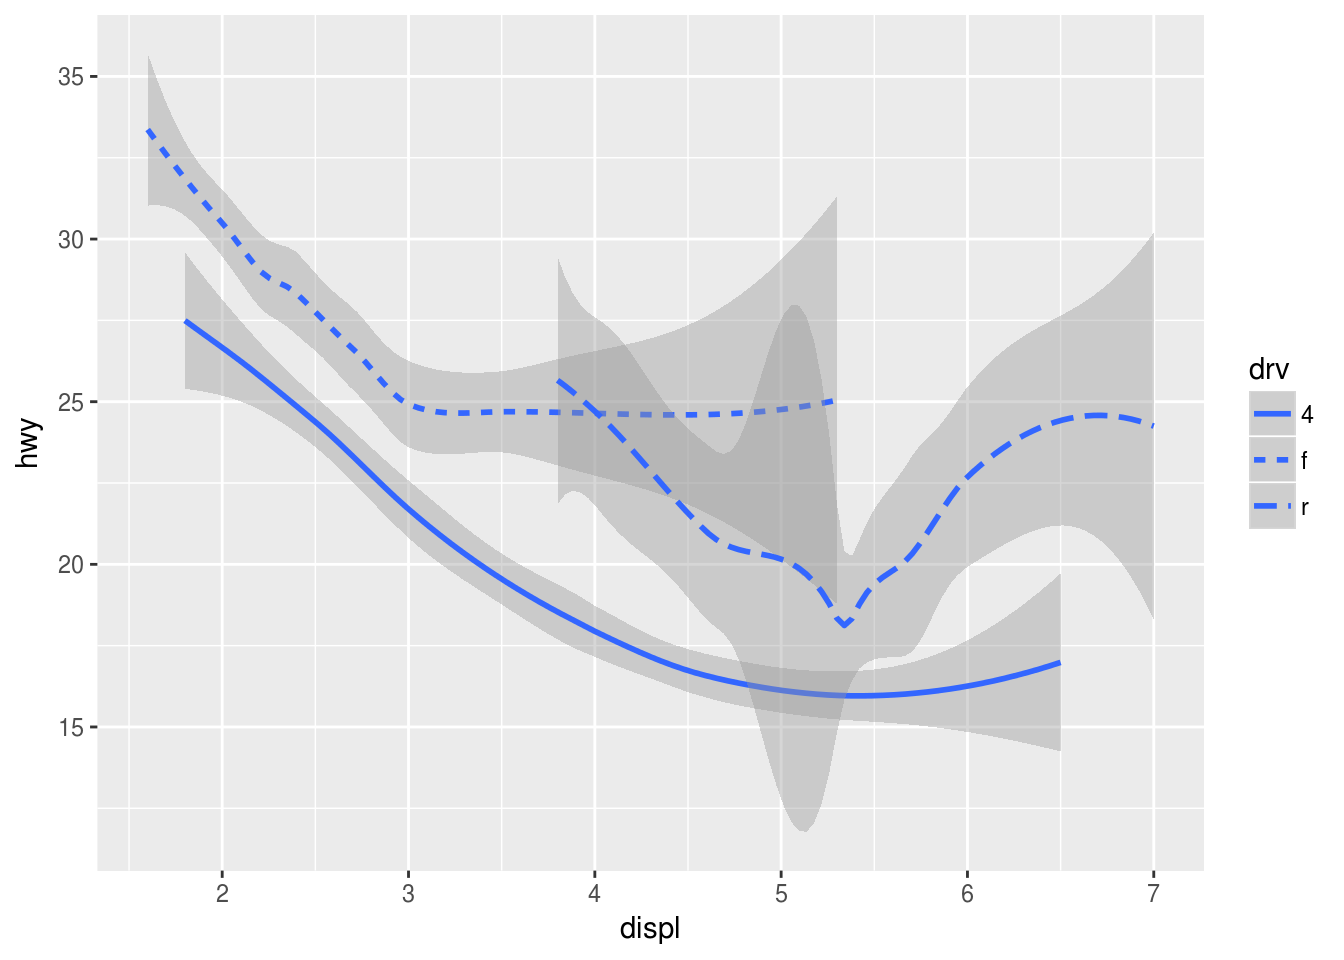
\includegraphics{Graficos_files/figure-latex/linetype-1.pdf}

Acá \texttt{geom\_smooth} separa tres líneas según el valor de
\texttt{drv}, que es la tracción. Una línea lisa para las que son 4x4
(4), rayas cortas para tracción delantera (f) y rayas largas para
tracción trasera (r).

Podemos ver más claramente porque tiene esta forma geom\_smooth
graficando los puntos de cada grupo:

\begin{figure}
\centering
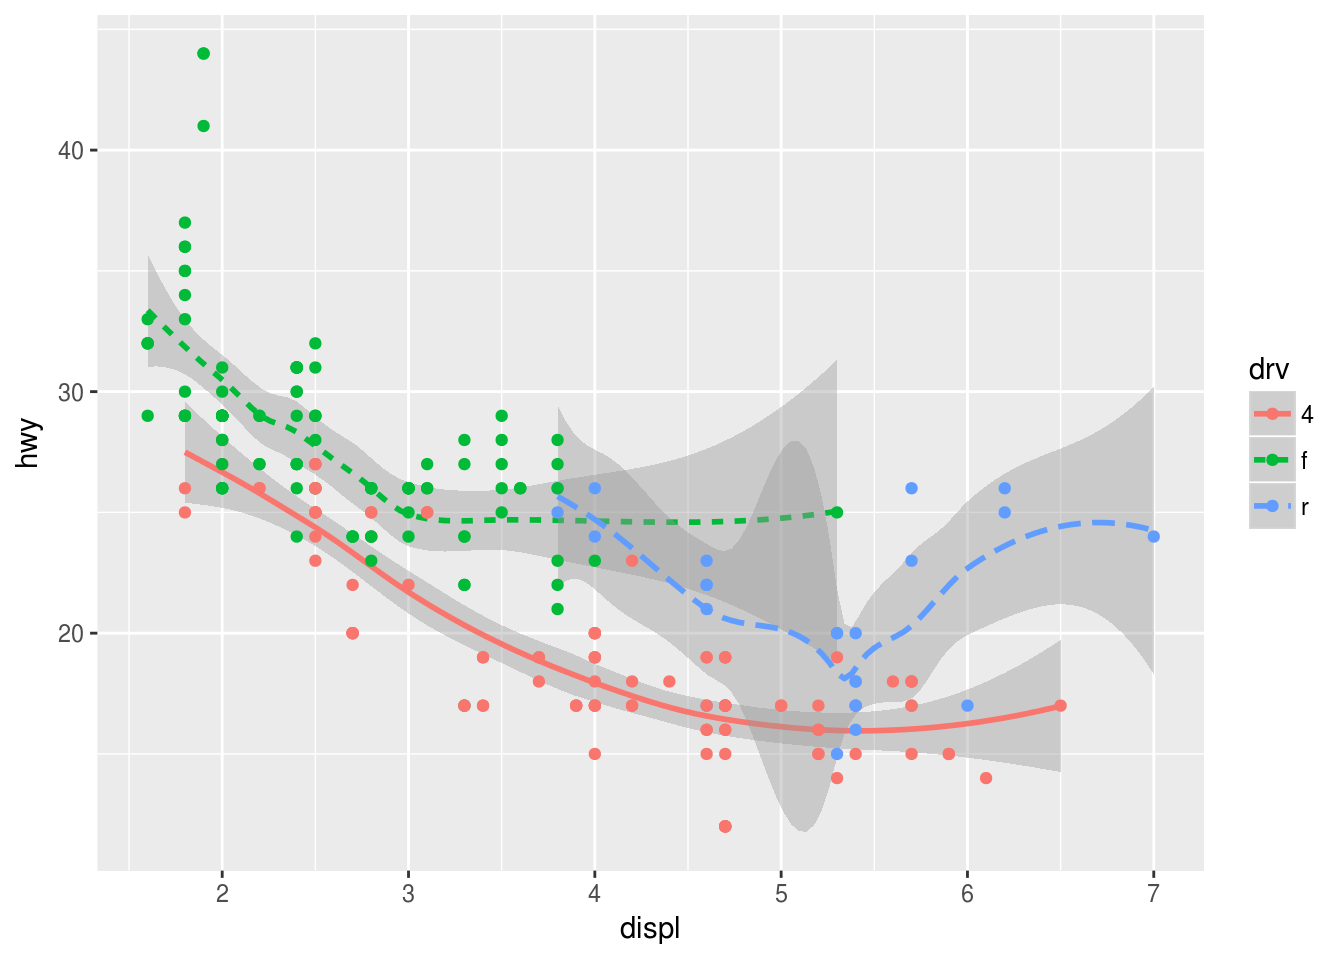
\includegraphics{Graficos_files/figure-latex/dos-geoms-2-1.pdf}
\caption{\label{fig:dos-geoms-2}Varios geoms pueden usarse en un mismo
gráfico.}
\end{figure}

Muchos \texttt{geoms} que resumen la información de varios datos con una
sola forma tienen un argumento de éstetica llamado \texttt{group} que
agrupa la observaciones que son iguales en una variable.

\begin{Shaded}
\begin{Highlighting}[]
\KeywordTok{ggplot}\NormalTok{(}\DataTypeTok{data =}\NormalTok{ mpg) }\OperatorTok{+}
\StringTok{  }\KeywordTok{geom_smooth}\NormalTok{(}\DataTypeTok{mapping =} \KeywordTok{aes}\NormalTok{(}\DataTypeTok{x =}\NormalTok{ displ, }\DataTypeTok{y =}\NormalTok{ hwy))}
              
\KeywordTok{ggplot}\NormalTok{(}\DataTypeTok{data =}\NormalTok{ mpg) }\OperatorTok{+}
\StringTok{  }\KeywordTok{geom_smooth}\NormalTok{(}\DataTypeTok{mapping =} \KeywordTok{aes}\NormalTok{(}\DataTypeTok{x =}\NormalTok{ displ, }\DataTypeTok{y =}\NormalTok{ hwy, }\DataTypeTok{group =}\NormalTok{ drv))}
    
\KeywordTok{ggplot}\NormalTok{(}\DataTypeTok{data =}\NormalTok{ mpg) }\OperatorTok{+}
\StringTok{  }\KeywordTok{geom_smooth}\NormalTok{(}
    \DataTypeTok{mapping =} \KeywordTok{aes}\NormalTok{(}\DataTypeTok{x =}\NormalTok{ displ, }\DataTypeTok{y =}\NormalTok{ hwy, }\DataTypeTok{color =}\NormalTok{ drv),}
    \DataTypeTok{show.legend =} \OtherTok{FALSE}
\NormalTok{  )}
\end{Highlighting}
\end{Shaded}

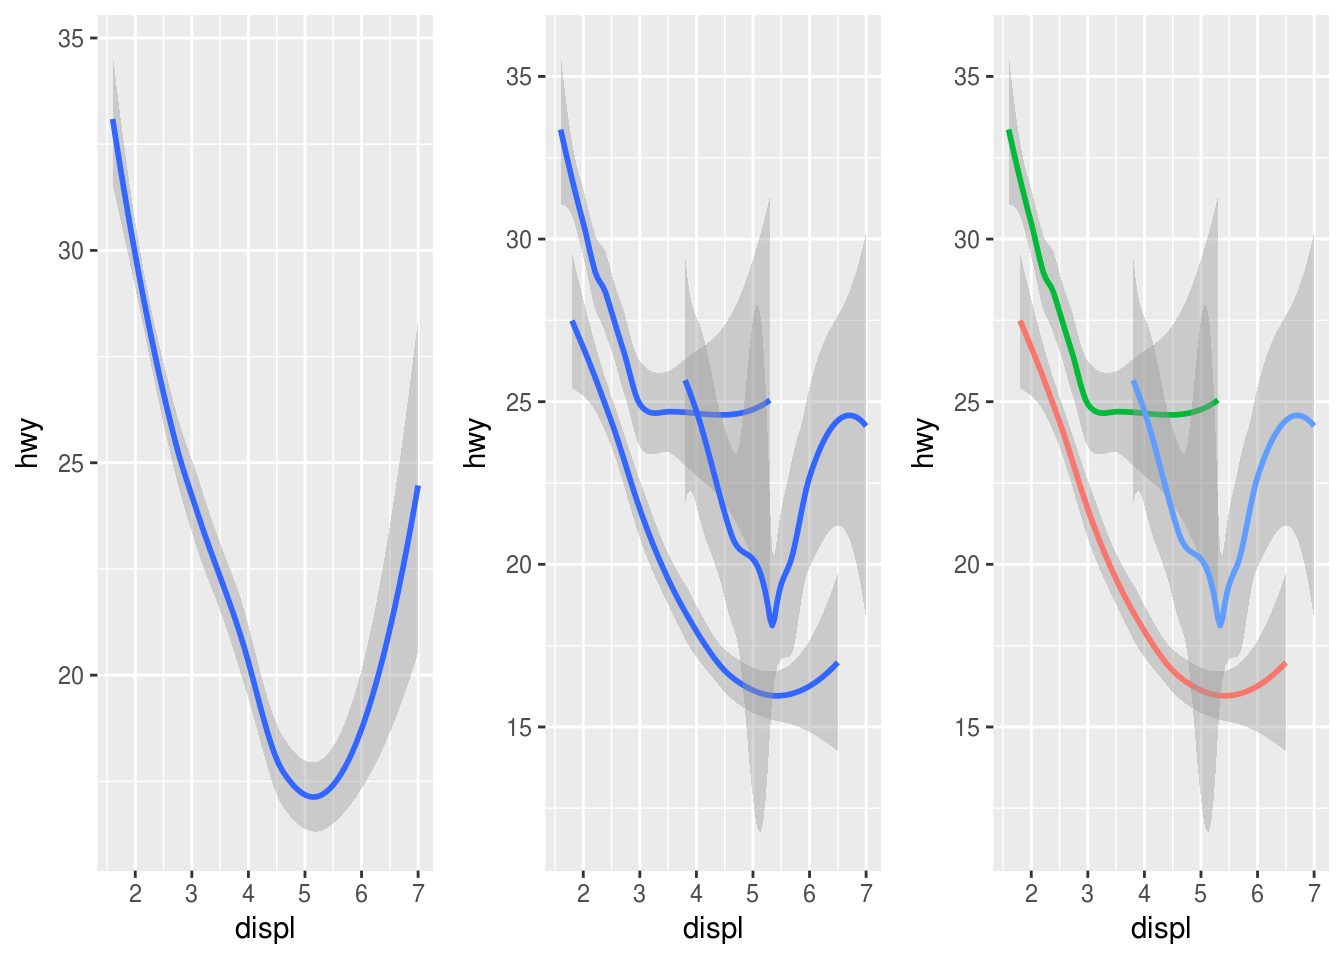
\includegraphics{Graficos_files/figure-latex/ejemplo-group-1.pdf}

Arriba vimos que podiamos usar dos geoms en un mismo gráfico (y
podríamos agregar más si quisieramos). Pero al hacerlo hemos duplicado
el \texttt{mapping} en los dos \texttt{geoms}:

\begin{Shaded}
\begin{Highlighting}[]
\KeywordTok{ggplot}\NormalTok{(}\DataTypeTok{data =}\NormalTok{ mpg) }\OperatorTok{+}\StringTok{ }
\StringTok{  }\KeywordTok{geom_smooth}\NormalTok{(}\DataTypeTok{mapping =} \KeywordTok{aes}\NormalTok{(}\DataTypeTok{x =}\NormalTok{ displ, }\DataTypeTok{y =}\NormalTok{ hwy, }\DataTypeTok{linetype =}\NormalTok{ drv, }\DataTypeTok{color =}\NormalTok{ drv)) }\OperatorTok{+}
\StringTok{  }\KeywordTok{geom_point}\NormalTok{(}\DataTypeTok{mapping =} \KeywordTok{aes}\NormalTok{(}\DataTypeTok{x =}\NormalTok{ displ, }\DataTypeTok{y =}\NormalTok{ hwy, }\DataTypeTok{color =}\NormalTok{ drv))}
\end{Highlighting}
\end{Shaded}

Podemos evitarlo si ponemos el \texttt{mapping} dentro de la llamada de
ggplot:

\begin{Shaded}
\begin{Highlighting}[]
\KeywordTok{ggplot}\NormalTok{(}\DataTypeTok{data =}\NormalTok{ mpg, }\DataTypeTok{mapping=}  \KeywordTok{aes}\NormalTok{(}\DataTypeTok{x =}\NormalTok{ displ, }\DataTypeTok{y =}\NormalTok{ hwy, }\DataTypeTok{linetype =}\NormalTok{ drv, }\DataTypeTok{color =}\NormalTok{ drv)) }\OperatorTok{+}\StringTok{ }
\StringTok{  }\KeywordTok{geom_smooth}\NormalTok{() }\OperatorTok{+}
\StringTok{  }\KeywordTok{geom_point}\NormalTok{()}
\end{Highlighting}
\end{Shaded}

Esto funciona porque las capas heredan el \texttt{mapping} de
\texttt{ggplot}. Por eso, va a funcionar en todas las capas que
pongamos, de forma \emph{global}. A veces, esto introduce ciertos
errores cuando usamos varias fuentes de datos y las variables no están
en presentes en todos los conjuntos. Es posible cambiar el
\texttt{mapping} de una capa específica y va a ser utilizada \emph{solo}
en esa capa; es decir, de forma de forma \emph{local}.

\begin{Shaded}
\begin{Highlighting}[]
\KeywordTok{ggplot}\NormalTok{(}\DataTypeTok{data =}\NormalTok{ mpg, }\DataTypeTok{mapping=}  \KeywordTok{aes}\NormalTok{(}\DataTypeTok{x =}\NormalTok{ displ, }\DataTypeTok{y =}\NormalTok{ hwy)) }\OperatorTok{+}\StringTok{ }
\StringTok{  }\KeywordTok{geom_smooth}\NormalTok{() }\OperatorTok{+}
\StringTok{  }\KeywordTok{geom_point}\NormalTok{(}\DataTypeTok{mapping =} \KeywordTok{aes}\NormalTok{(}\DataTypeTok{color =}\NormalTok{ class))}
\end{Highlighting}
\end{Shaded}

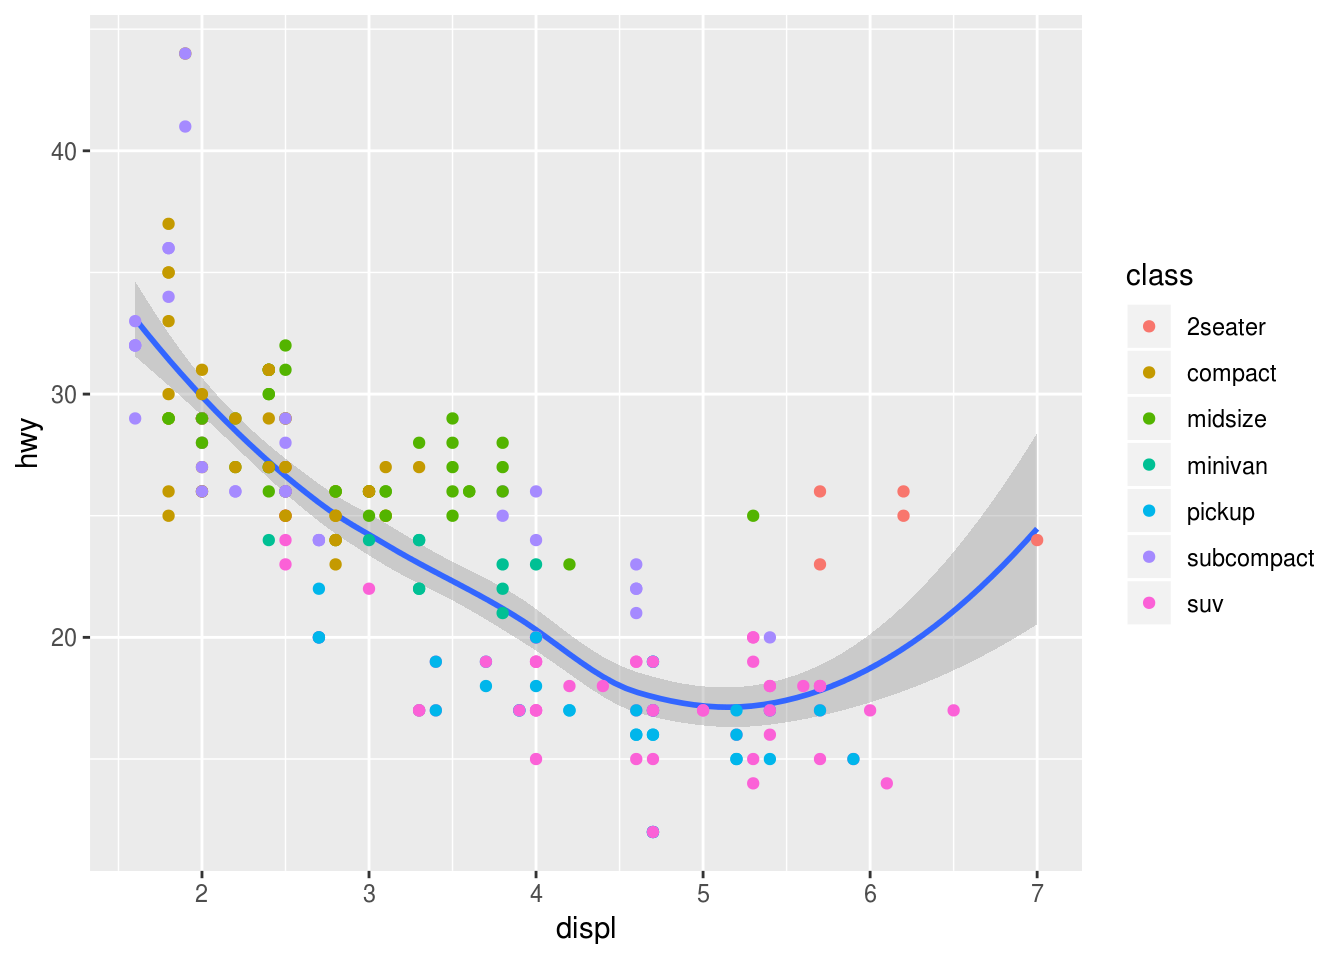
\includegraphics{Graficos_files/figure-latex/mapping-ggplot-resumido-1.pdf}

O también podemos definir otro conjunto de datos para el \texttt{geom}:

\begin{Shaded}
\begin{Highlighting}[]
\KeywordTok{ggplot}\NormalTok{(}\DataTypeTok{data =}\NormalTok{ mpg, }\DataTypeTok{mapping =} \KeywordTok{aes}\NormalTok{(}\DataTypeTok{x =}\NormalTok{ displ, }\DataTypeTok{y =}\NormalTok{ hwy)) }\OperatorTok{+}\StringTok{ }
\StringTok{  }\KeywordTok{geom_point}\NormalTok{(}\DataTypeTok{mapping =} \KeywordTok{aes}\NormalTok{(}\DataTypeTok{color =}\NormalTok{ class)) }\OperatorTok{+}\StringTok{ }
\StringTok{  }\KeywordTok{geom_smooth}\NormalTok{(}\DataTypeTok{data =} \KeywordTok{filter}\NormalTok{(mpg, class }\OperatorTok{==}\StringTok{ "subcompact"}\NormalTok{), }\DataTypeTok{se =} \OtherTok{FALSE}\NormalTok{)}
\end{Highlighting}
\end{Shaded}

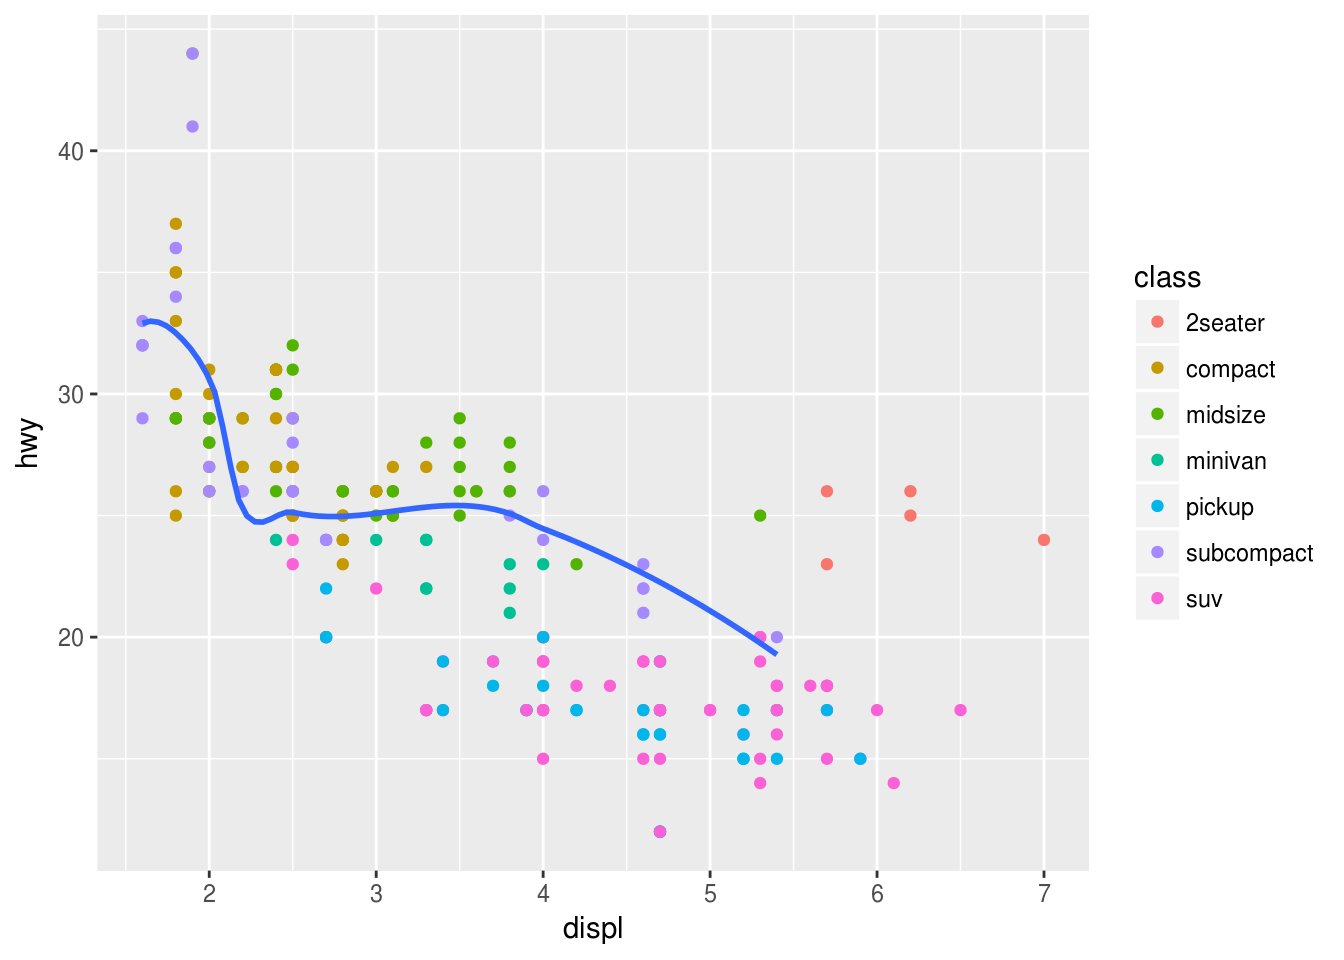
\includegraphics{Graficos_files/figure-latex/other-data-1.pdf}

Todavía no vieron \texttt{filter}, pero ya lo verán más adelante.

\hypertarget{transformaciones-estadisticas}{%
\section{Transformaciones
Estadísticas}\label{transformaciones-estadisticas}}

Pensemos en los gráficos de barras. En \texttt{ggplot2} se hacen con
\texttt{geom\_bar}. A primera vista los gráficos de barras parecen
simples. En este caso estamos graficando datos de diamantes, del
conjunto de datos \texttt{diamonds} que contiene cerca 54000 datos. En
el gráfico vemos que hay muchos más diamantes de cortes buenos que
regulares.

\begin{Shaded}
\begin{Highlighting}[]
\KeywordTok{ggplot}\NormalTok{(}\DataTypeTok{data =}\NormalTok{ diamonds) }\OperatorTok{+}
\StringTok{  }\KeywordTok{geom_bar}\NormalTok{(}\DataTypeTok{mapping =} \KeywordTok{aes}\NormalTok{(}\DataTypeTok{x =}\NormalTok{ cut))}
\end{Highlighting}
\end{Shaded}

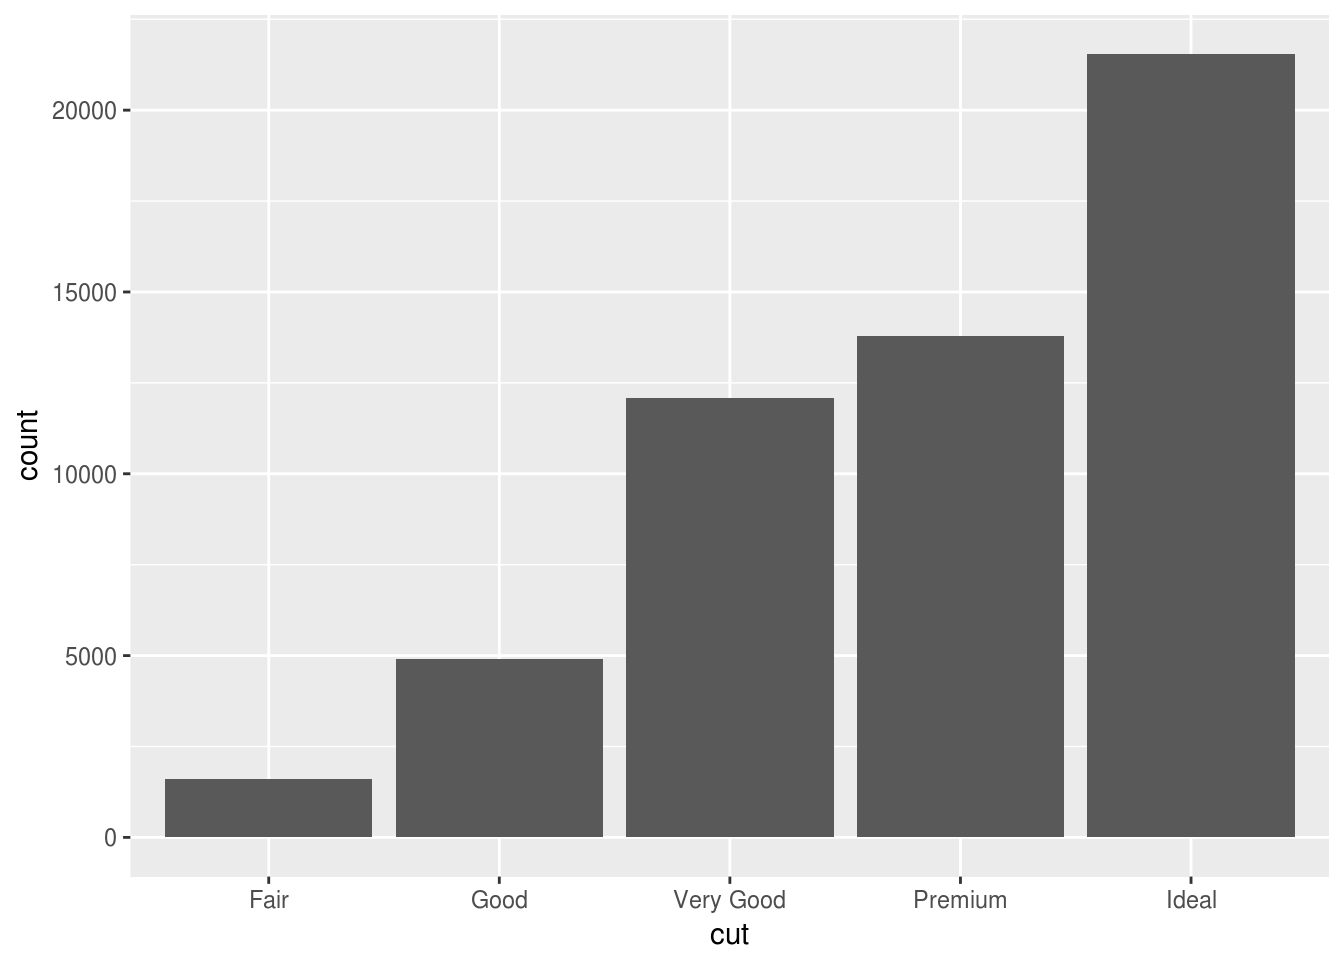
\includegraphics{Graficos_files/figure-latex/geom-bar-1.pdf}

En el eje \emph{x} está puesto el corte, y en el eje \emph{y} está
puesto la cuenta (frecuencia) de cada uno. Pero si vemos el conjunto de
datos veremos que esta última ¡no está! Entonces ¿De dónde salió?
Algunos \emph{geoms} grafican los datos puros pero otros aplican
transformaciones estadísticas a los datos y crean nuevas variables:

\begin{itemize}
\tightlist
\item
  Los gráficos de barras, histograms y polígonos de frecuencia cuentan y
  juntan los datos.
\item
  \texttt{geom\_smooth} usa modelos para mostrar las tendencias de los
  datos.
\item
  \texttt{geom\_boxplot} crea un sumario de estadísticos robustos para
  mostrar los datos.
\end{itemize}

El algoritmo usado para calcular las nuevas variables se llama
\texttt{stat}. Abajo vemos como funciona \texttt{stat\_count}

Empieza con los datos

\begin{verbatim}
## # A tibble: 6 x 10
##   carat cut       color clarity depth table price     x     y     z
##   <dbl> <ord>     <ord> <ord>   <dbl> <dbl> <int> <dbl> <dbl> <dbl>
## 1 0.230 Ideal     E     SI2      61.5   55.   326  3.95  3.98  2.43
## 2 0.210 Premium   E     SI1      59.8   61.   326  3.89  3.84  2.31
## 3 0.230 Good      E     VS1      56.9   65.   327  4.05  4.07  2.31
## 4 0.290 Premium   I     VS2      62.4   58.   334  4.20  4.23  2.63
## 5 0.310 Good      J     SI2      63.3   58.   335  4.34  4.35  2.75
## 6 0.240 Very Good J     VVS2     62.8   57.   336  3.94  3.96  2.48
\end{verbatim}

\texttt{geom\_bar} calcula las nuevas variables usando el \texttt{stat}
\texttt{count} que devuelve un nuevo data.frame

\begin{verbatim}
## # A tibble: 5 x 3
##   cut       count  prop
##   <ord>     <int> <dbl>
## 1 Fair       1610    1.
## 2 Good       4906    1.
## 3 Very Good 12082    1.
## 4 Premium   13791    1.
## 5 Ideal     21551    1.
\end{verbatim}

\texttt{geom\_bar} luego usa esos datos para graficar:

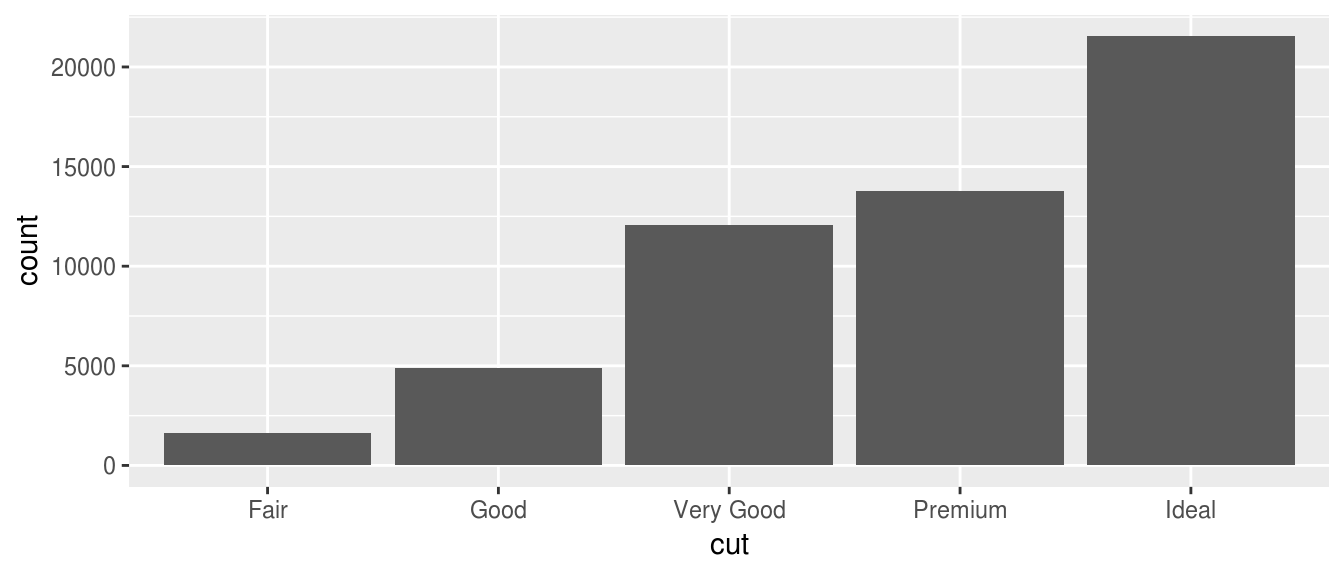
\includegraphics{Graficos_files/figure-latex/geom-bar-diamonds-1.pdf}

Podés saber que \texttt{stat} usa cada \texttt{geom} usando la ayuda.
Por ejemplo, \texttt{?geom\_bar} usa por defecto \texttt{stat\_count} y
\texttt{stat\_count} usa por defecto \texttt{geom\_bar} para mostrar sus
resultados y ambos están descriptos en la misma página de ayuda. Podemos
ver que es calculado en la sección \emph{Computed Variables}.

Es posible intercambiar \texttt{geom} por su \texttt{stat}. Por ejemplo:

\begin{Shaded}
\begin{Highlighting}[]
\KeywordTok{ggplot}\NormalTok{(}\DataTypeTok{data =}\NormalTok{ diamonds) }\OperatorTok{+}
\StringTok{  }\KeywordTok{stat_count}\NormalTok{(}\DataTypeTok{mapping =} \KeywordTok{aes}\NormalTok{(}\DataTypeTok{x =}\NormalTok{ cut))}
\end{Highlighting}
\end{Shaded}

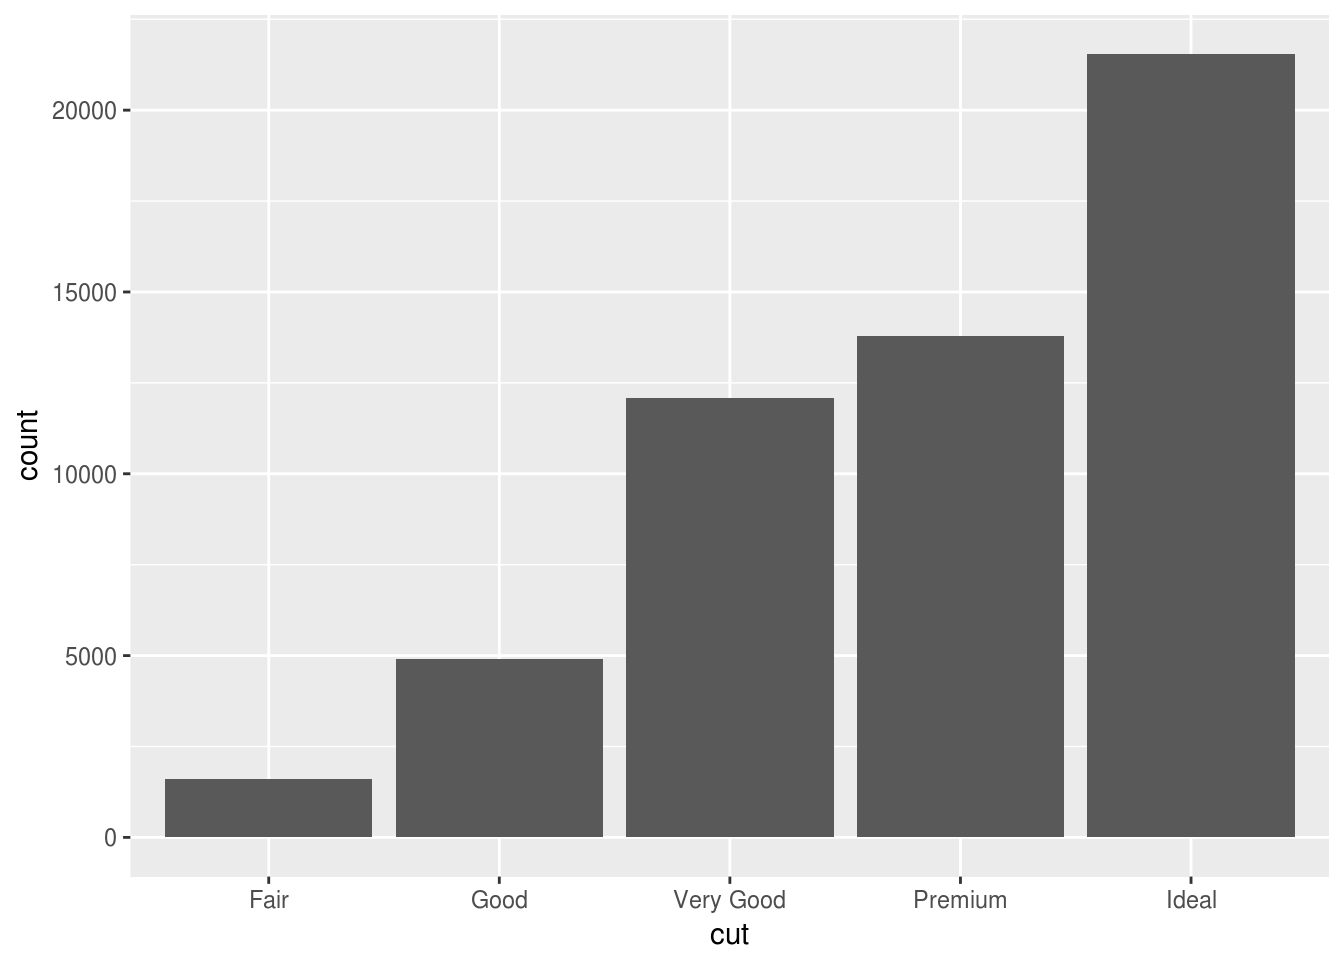
\includegraphics{Graficos_files/figure-latex/stat-count-1.pdf}

Esto funciona porque cada \emph{stat} tiene un \emph{geom} por defecto y
cada \emph{geom} tiene un \emph{stat}. Lo que significa que podes usar
cada \emph{geom} sin preocuparte por las transformaciones subyacentes.

Hay veces que querrás cambiar los valores por defecto:

\begin{enumerate}
\def\labelenumi{\arabic{enumi}.}
\tightlist
\item
  Cuando tengas las variables precomputadas y desees graficarlas. En el
  código de abajo cambio el \emph{stat} de \texttt{geom\_bar} por
  \texttt{stat\_identity} (identidad). Esto me permite graficar la
  altura de la variable \emph{y} a algún valor del conjunto de datos.
\end{enumerate}

\begin{Shaded}
\begin{Highlighting}[]
\NormalTok{demo <-}\StringTok{ }\KeywordTok{tribble}\NormalTok{(}
  \OperatorTok{~}\NormalTok{cut,         }\OperatorTok{~}\NormalTok{freq,}
  \StringTok{"Fair"}\NormalTok{,       }\DecValTok{1610}\NormalTok{,}
  \StringTok{"Good"}\NormalTok{,       }\DecValTok{4906}\NormalTok{,}
  \StringTok{"Very Good"}\NormalTok{,  }\DecValTok{12082}\NormalTok{,}
  \StringTok{"Premium"}\NormalTok{,    }\DecValTok{13791}\NormalTok{,}
  \StringTok{"Ideal"}\NormalTok{,      }\DecValTok{21551}
\NormalTok{)}

\KeywordTok{ggplot}\NormalTok{(}\DataTypeTok{data =}\NormalTok{ demo) }\OperatorTok{+}
\StringTok{  }\KeywordTok{geom_bar}\NormalTok{(}\DataTypeTok{mapping =} \KeywordTok{aes}\NormalTok{(}\DataTypeTok{x =}\NormalTok{ cut, }\DataTypeTok{y =}\NormalTok{ freq), }\DataTypeTok{stat =} \StringTok{"identity"}\NormalTok{)}
\end{Highlighting}
\end{Shaded}

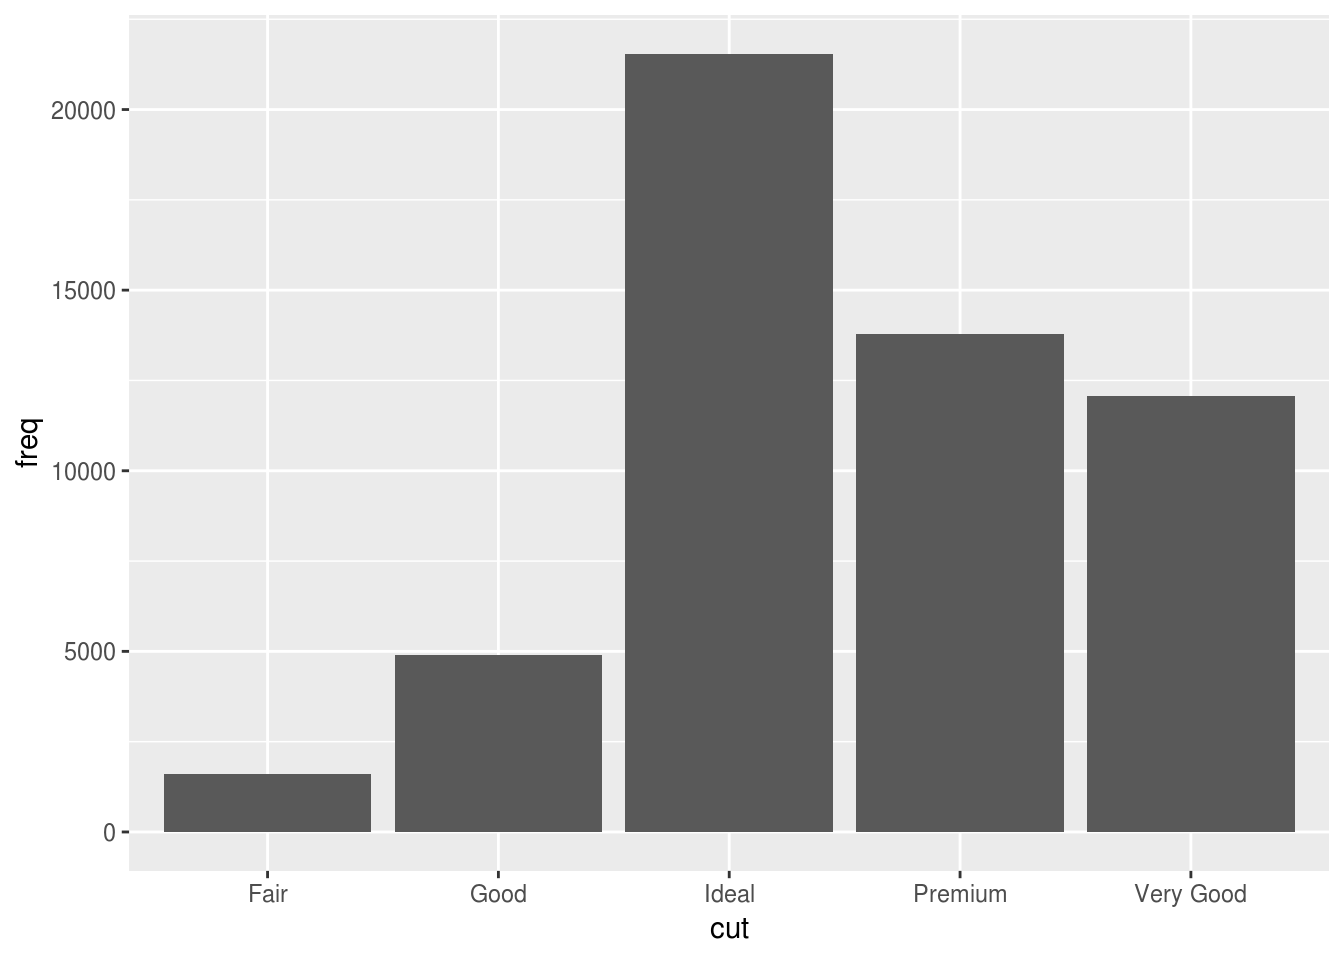
\includegraphics{Graficos_files/figure-latex/summary-data-1.pdf}

No te preocupes si no entiendes que hace \texttt{tribble} o
\texttt{\textless{}-}. Todavía no lo hemos visto pero quizá puedas
entender que hacen por su contexto

\begin{enumerate}
\def\labelenumi{\arabic{enumi}.}
\setcounter{enumi}{1}
\tightlist
\item
  Muchos \emph{stats} computan varias variables y quizás quieras mostrar
  otra. Abajo, en lugar de graficar la frecuencia o cuenta, grafico la
  proporción o frecuencia relativa.
\end{enumerate}

\begin{Shaded}
\begin{Highlighting}[]
\KeywordTok{ggplot}\NormalTok{(}\DataTypeTok{data =}\NormalTok{ diamonds) }\OperatorTok{+}
\StringTok{  }\KeywordTok{geom_bar}\NormalTok{(}\DataTypeTok{mapping =} \KeywordTok{aes}\NormalTok{(}\DataTypeTok{x =}\NormalTok{ cut, }\DataTypeTok{y =}\NormalTok{ ..prop.., }\DataTypeTok{group =} \DecValTok{1}\NormalTok{))}
\end{Highlighting}
\end{Shaded}

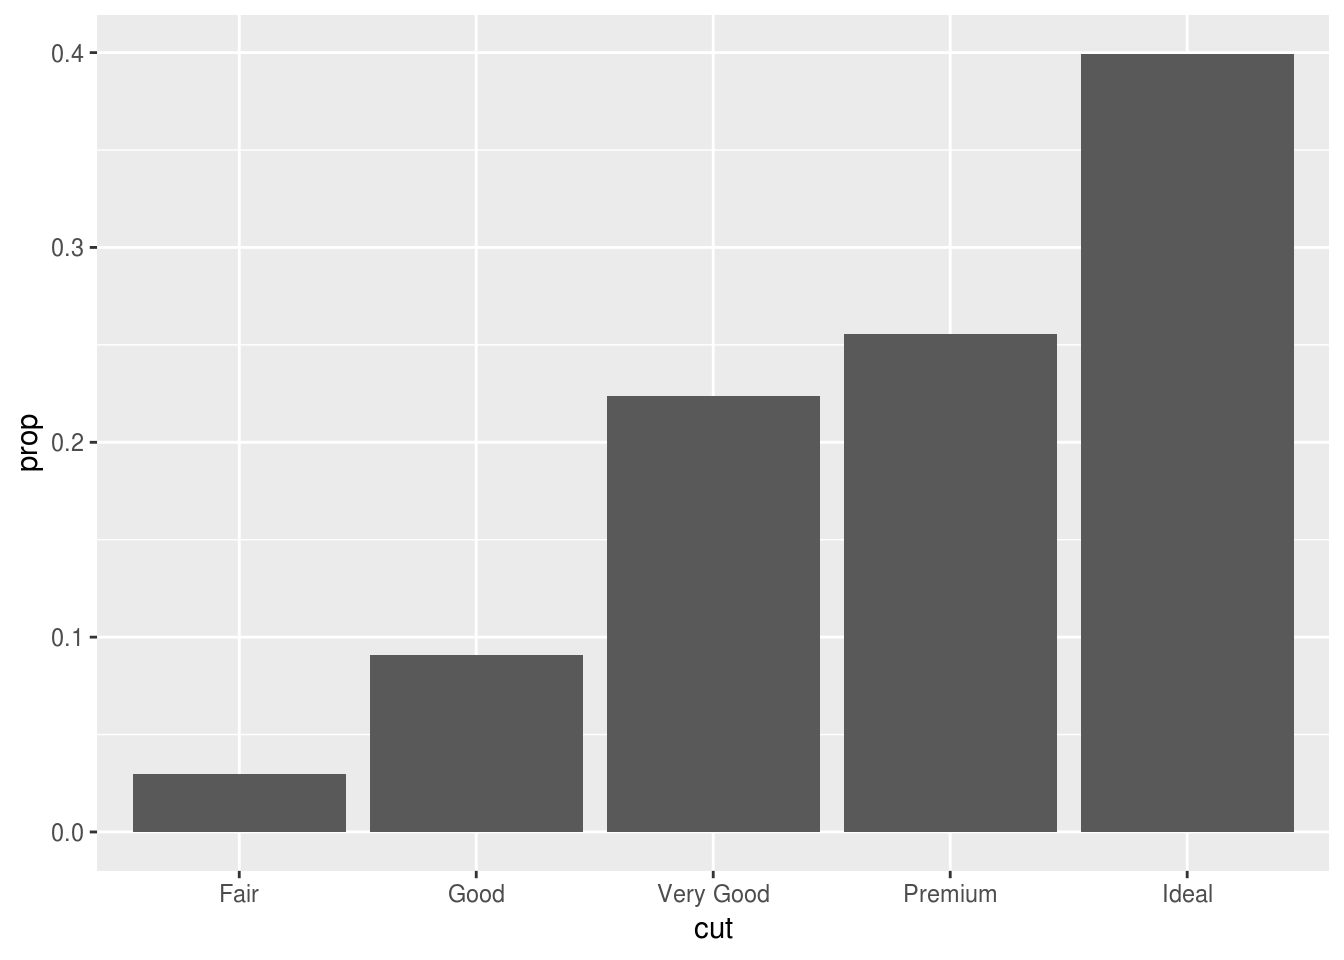
\includegraphics{Graficos_files/figure-latex/prop-1.pdf}

\begin{enumerate}
\def\labelenumi{\arabic{enumi}.}
\setcounter{enumi}{2}
\tightlist
\item
  Quizás quieras llamar la atención sobre ciertos medidas de resumen que
  has calculado. Puedes hacer esto con \texttt{stat\_summary}.
\end{enumerate}

\begin{Shaded}
\begin{Highlighting}[]
\KeywordTok{ggplot}\NormalTok{(}\DataTypeTok{data =}\NormalTok{ diamonds) }\OperatorTok{+}
\StringTok{  }\KeywordTok{stat_summary}\NormalTok{(}
    \DataTypeTok{mapping =} \KeywordTok{aes}\NormalTok{(}\DataTypeTok{x =}\NormalTok{ cut, }\DataTypeTok{y =}\NormalTok{ depth),}
    \DataTypeTok{fun.y =}\NormalTok{ median,}
    \DataTypeTok{fun.ymax =}\NormalTok{ max,}
    \DataTypeTok{fun.ymin =}\NormalTok{ min}
    
\NormalTok{  )}
\end{Highlighting}
\end{Shaded}

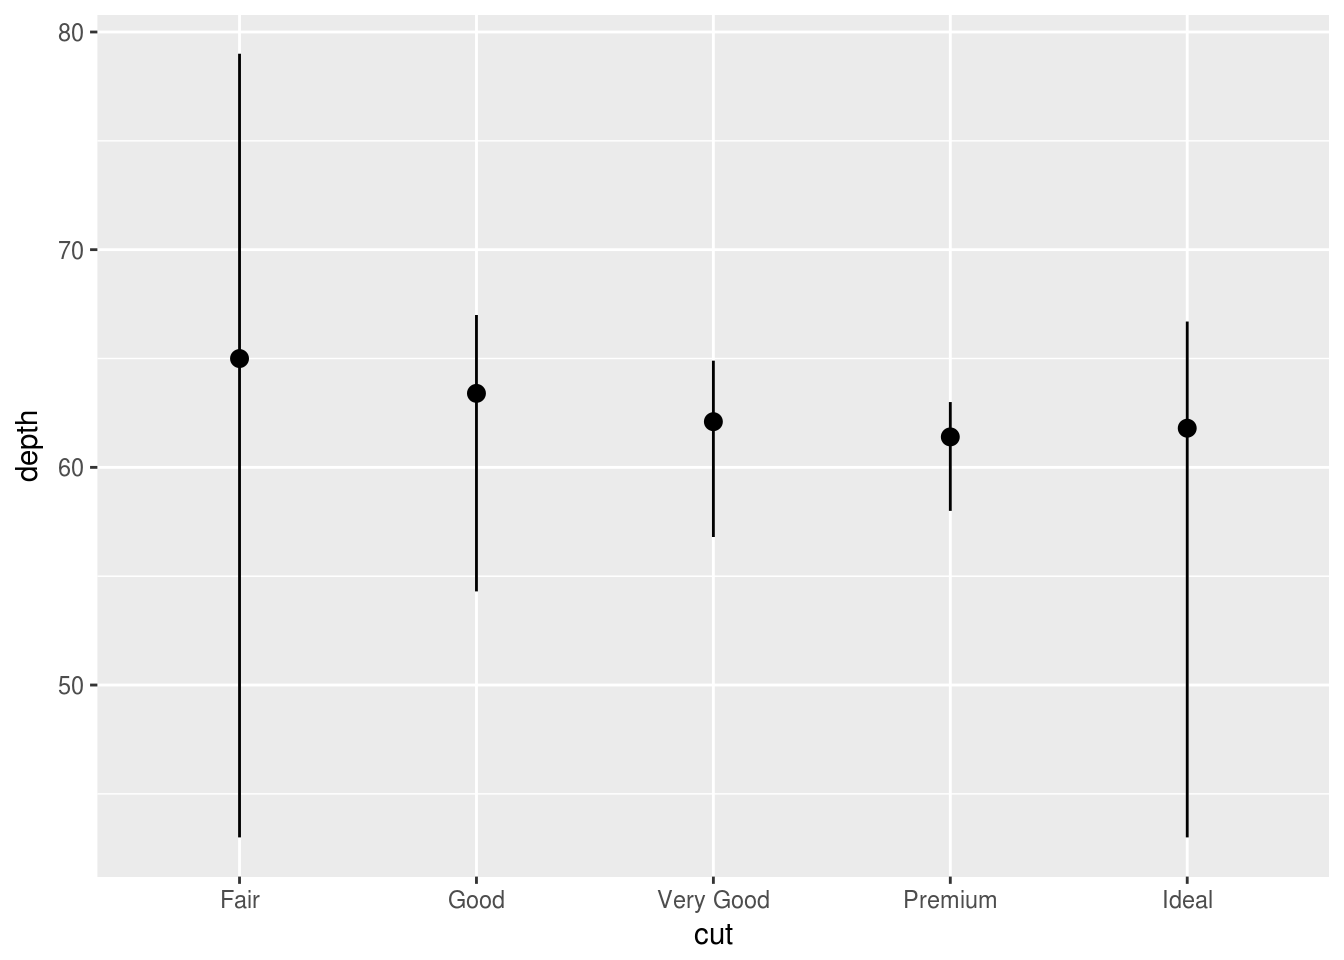
\includegraphics{Graficos_files/figure-latex/unnamed-chunk-6-1.pdf}

\hypertarget{ajuste-de-posiciones}{%
\section{Ajuste de Posiciones}\label{ajuste-de-posiciones}}

El gráfico anterior revela algo interesante de los gráficos de barras.
Tienen relleno (\emph{fill}) y tienen color.

\begin{Shaded}
\begin{Highlighting}[]
\KeywordTok{ggplot}\NormalTok{(}\DataTypeTok{data =}\NormalTok{ diamonds) }\OperatorTok{+}\StringTok{ }
\StringTok{  }\KeywordTok{geom_bar}\NormalTok{(}\DataTypeTok{mapping =} \KeywordTok{aes}\NormalTok{(}\DataTypeTok{x =}\NormalTok{ cut, }\DataTypeTok{fill =}\NormalTok{ clarity))}
\end{Highlighting}
\end{Shaded}

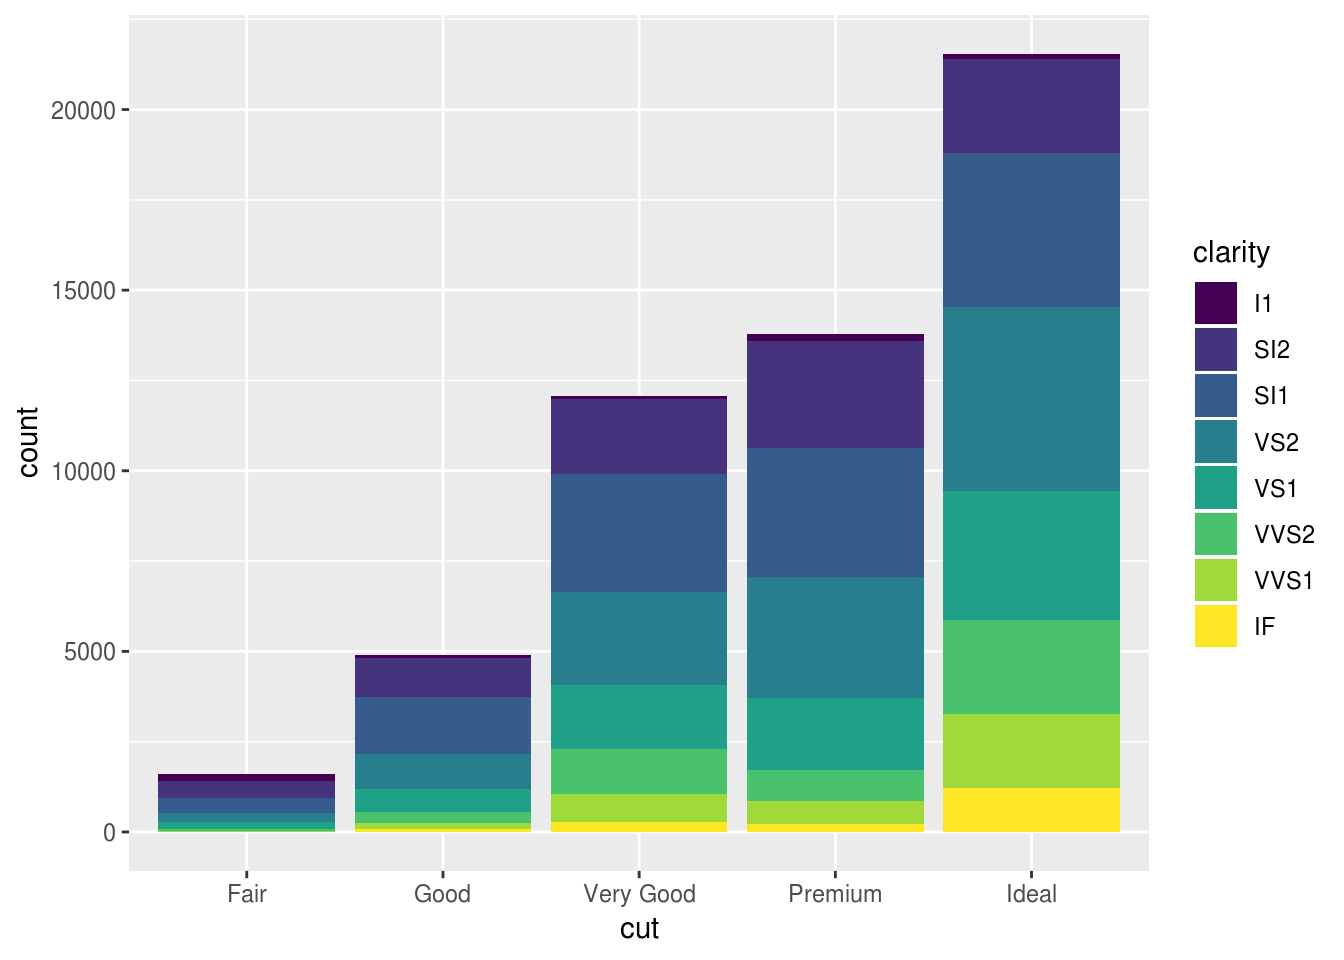
\includegraphics{Graficos_files/figure-latex/fill-1.pdf}

\begin{Shaded}
\begin{Highlighting}[]
\KeywordTok{ggplot}\NormalTok{(}\DataTypeTok{data =}\NormalTok{ diamonds) }\OperatorTok{+}\StringTok{ }
\StringTok{  }\KeywordTok{geom_bar}\NormalTok{(}\DataTypeTok{mapping =} \KeywordTok{aes}\NormalTok{(}\DataTypeTok{x =}\NormalTok{ cut, }\DataTypeTok{color =}\NormalTok{ clarity))}
\end{Highlighting}
\end{Shaded}

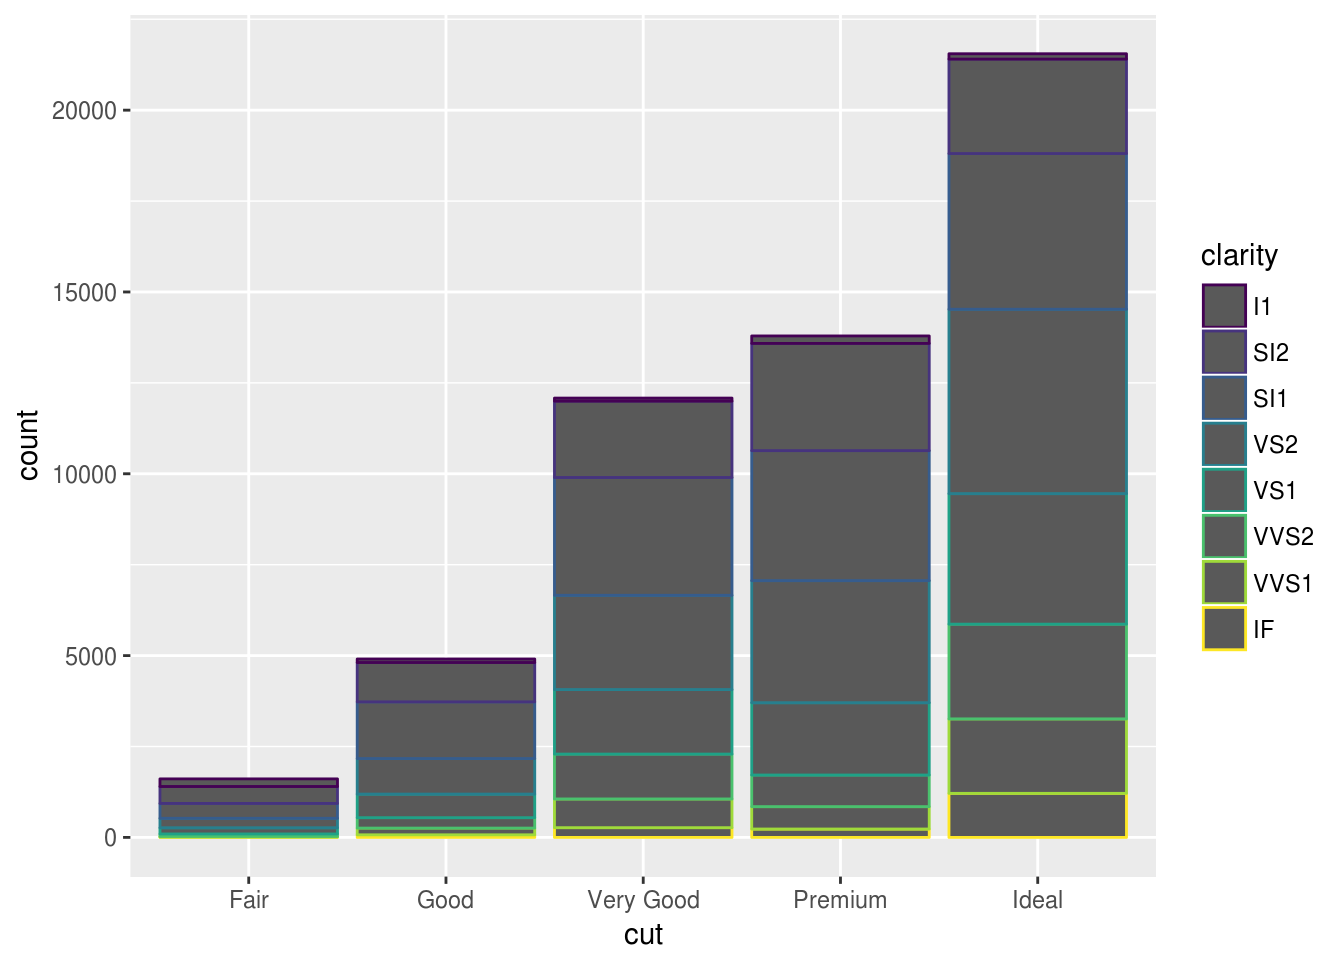
\includegraphics{Graficos_files/figure-latex/fill-2.pdf}

Es más claro trabajar con el relleno porque es más visible en el
gráfico. Pero vemos que las distintas barras están apiladas, lo que
dificulta la comparación. Se debe a que la posición de barras es apilada
(\texttt{stack}) por defecto. Podemos cambiarla modificando el argumento
\texttt{position} de \texttt{geom\_bar()}. Entre las otras posiciones
que podemos elegir están identidad (\texttt{identity}), esquivar
(\texttt{dodge}) y relleno (\texttt{fill}) .

\begin{itemize}
\tightlist
\item
  Identidad hace que las barras (o otro \emph{geoms}) caigan unas
  encimas de otras. No es muy útil porque las barras se superponen y
  hace muy difícil la interpretación. Se puede mejorar agregando
  transparencia y usando color y no relleno, pero es complicado de
  interpetar si la barras se superponen o están apiladas.
\end{itemize}

\begin{Shaded}
\begin{Highlighting}[]
\KeywordTok{ggplot}\NormalTok{(}\DataTypeTok{data =}\NormalTok{ diamonds) }\OperatorTok{+}\StringTok{ }
\StringTok{   }\KeywordTok{geom_bar}\NormalTok{(}\DataTypeTok{mapping =} \KeywordTok{aes}\NormalTok{(}\DataTypeTok{x =}\NormalTok{ cut, }\DataTypeTok{color =}\NormalTok{ clarity), }\DataTypeTok{position =} \StringTok{"identity"}\NormalTok{)}
\end{Highlighting}
\end{Shaded}

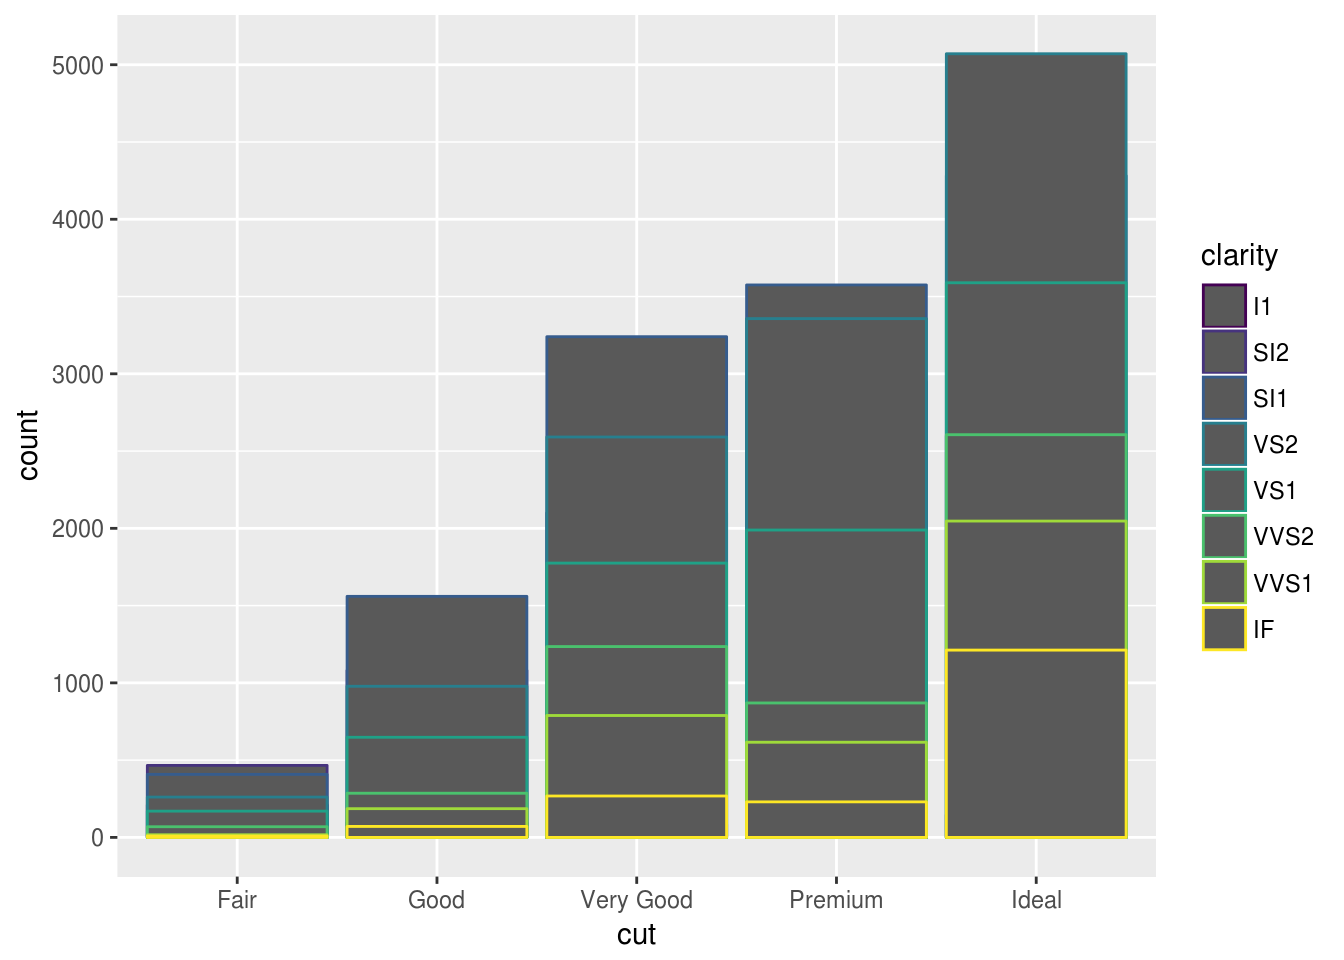
\includegraphics{Graficos_files/figure-latex/pos-identity-1.pdf}

\begin{itemize}
\tightlist
\item
  Esquivar es quizás la más útil junto con relleno. Hace que las barras
  estén una al lado de la otra. Lo que hace que sea sencillo comparar la
  altura de estas.
\end{itemize}

\begin{Shaded}
\begin{Highlighting}[]
\KeywordTok{ggplot}\NormalTok{(}\DataTypeTok{data =}\NormalTok{ diamonds) }\OperatorTok{+}\StringTok{ }
\StringTok{   }\KeywordTok{geom_bar}\NormalTok{(}\DataTypeTok{mapping =} \KeywordTok{aes}\NormalTok{(}\DataTypeTok{x =}\NormalTok{ cut, }\DataTypeTok{fill =}\NormalTok{ clarity), }\DataTypeTok{position =} \StringTok{"dodge"}\NormalTok{)}
\end{Highlighting}
\end{Shaded}

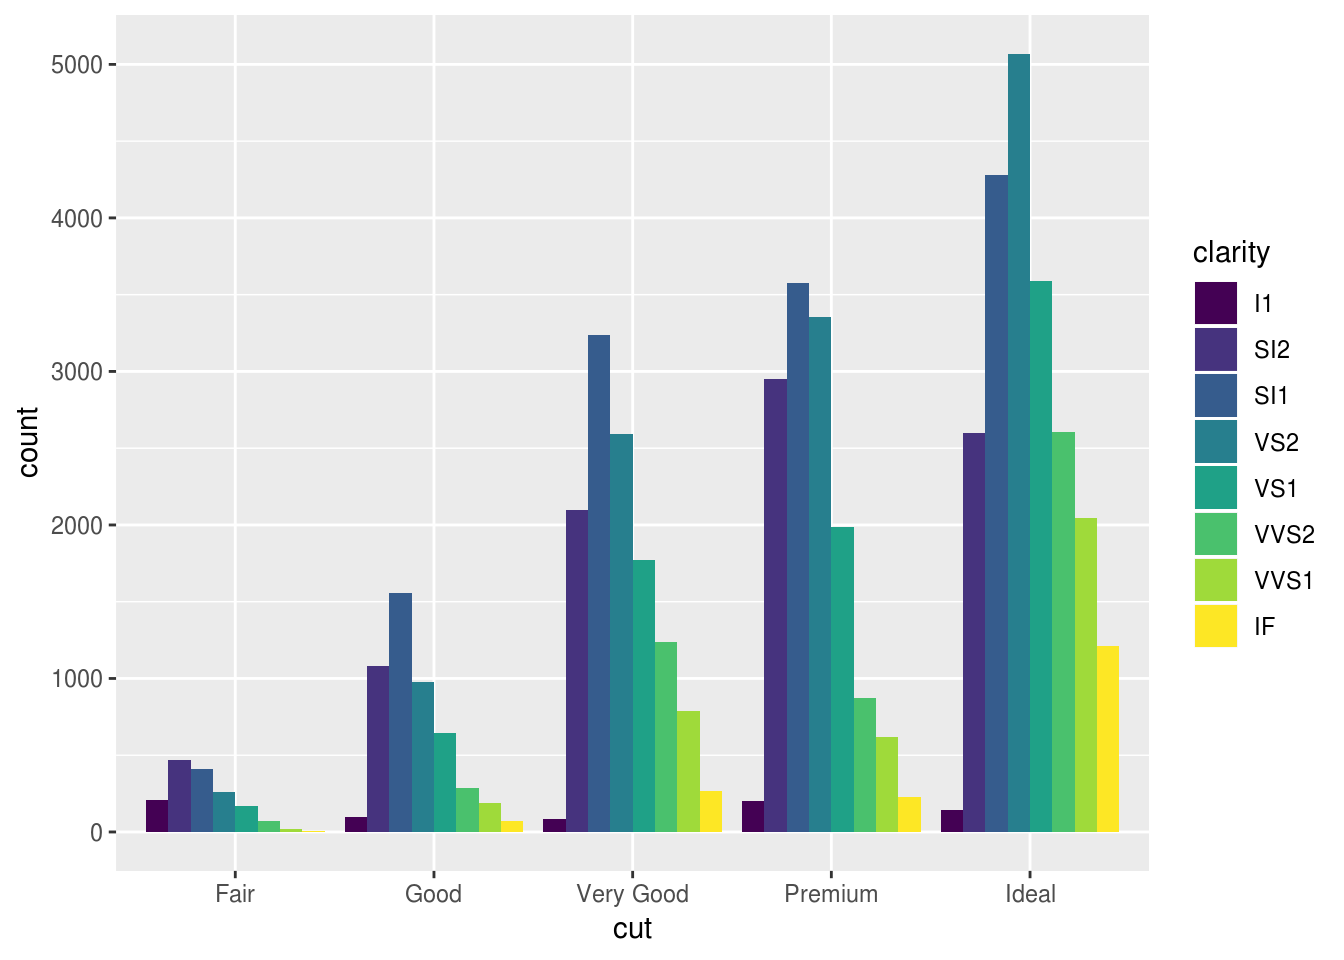
\includegraphics{Graficos_files/figure-latex/pos-dodge-1.pdf}

\begin{itemize}
\tightlist
\item
  Recién vimos que que con esquivar podemos poner las barras una al lado
  de otra. Pero, más allá de comparar la cantidad de diamantes en cada
  uno, ya que la cantidad es muy diferente en cada corte resulta más
  útil comparar las proporciones de cada una de las claridades. Relleno
  funciona de forma similar al apilado, pero estadariza cada columna a
  longitud uno. Entonces se ve las proporciones o frecuencias relativas
  de cada uno de los niveles de \texttt{clarity}.
\end{itemize}

\begin{Shaded}
\begin{Highlighting}[]
\KeywordTok{ggplot}\NormalTok{(}\DataTypeTok{data =}\NormalTok{ diamonds) }\OperatorTok{+}\StringTok{ }
\StringTok{   }\KeywordTok{geom_bar}\NormalTok{(}\DataTypeTok{mapping =} \KeywordTok{aes}\NormalTok{(}\DataTypeTok{x =}\NormalTok{ cut, }\DataTypeTok{fill =}\NormalTok{ clarity), }\DataTypeTok{position =} \StringTok{"fill"}\NormalTok{)}
\end{Highlighting}
\end{Shaded}

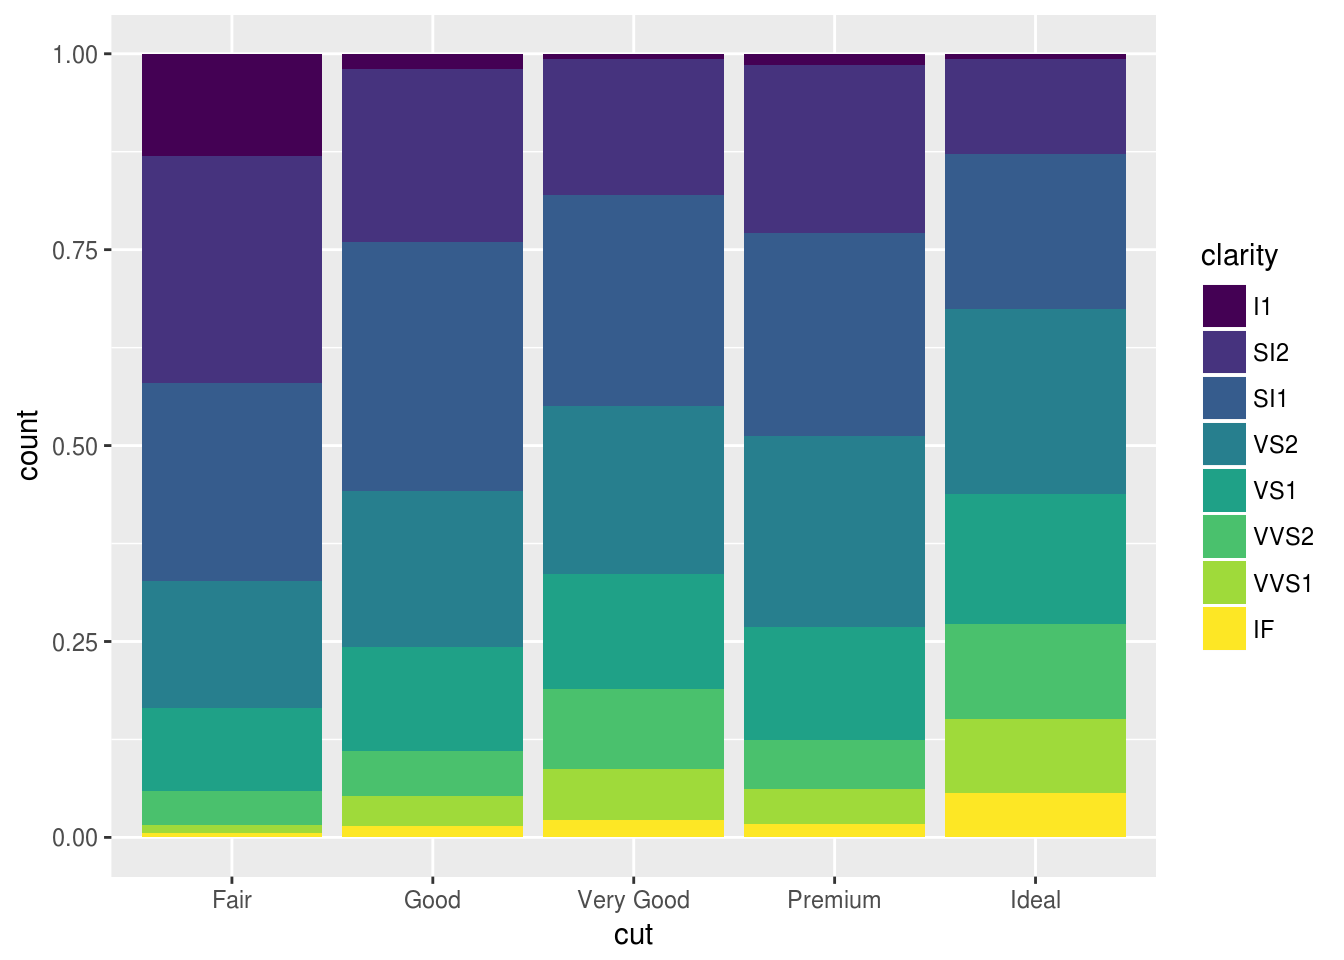
\includegraphics{Graficos_files/figure-latex/pos-fill-1.pdf}

Hay otros ajustes de posiciones que no son útiles para los gráficos de
barras pero son muy útiles para los gráficos de puntos. En el gráfico de
dispersión entre \texttt{displ} y \texttt{hwy} hay menos puntos que el
total 31 vs 234. Muchos puntos se superponen, por eso vemos menos.
Podemos evitarlo añadiendo un poco de movimiento aleatorio a cada punto.

\begin{Shaded}
\begin{Highlighting}[]
\KeywordTok{ggplot}\NormalTok{(}\DataTypeTok{data =}\NormalTok{ mpg) }\OperatorTok{+}
\StringTok{  }\KeywordTok{geom_point}\NormalTok{(}\DataTypeTok{mapping =} \KeywordTok{aes}\NormalTok{(}\DataTypeTok{x =}\NormalTok{ displ, }\DataTypeTok{y =}\NormalTok{ hwy), }\DataTypeTok{position =} \StringTok{"jitter"}\NormalTok{)}
\end{Highlighting}
\end{Shaded}

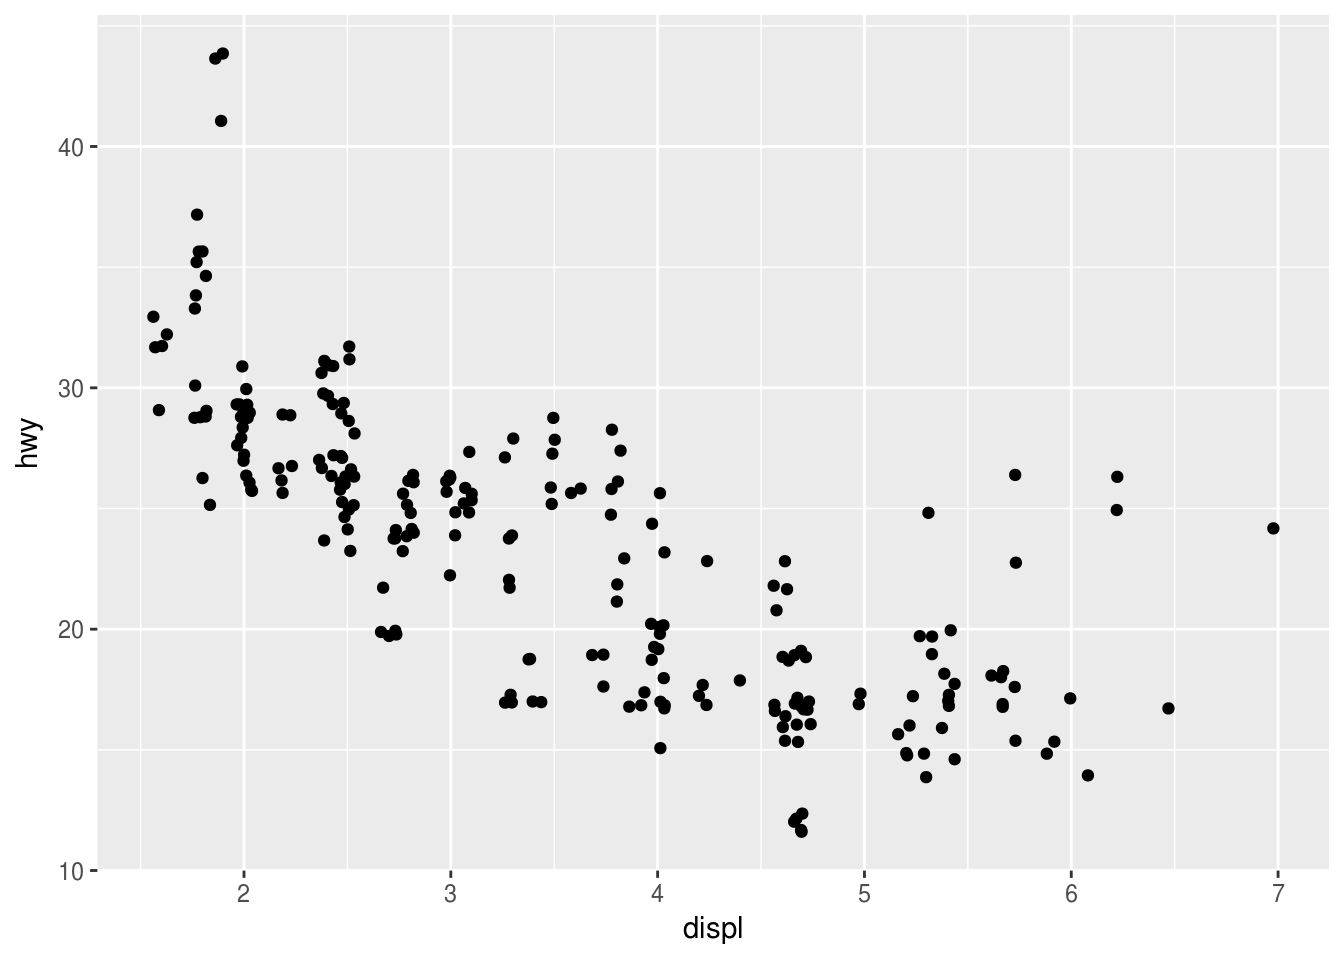
\includegraphics{Graficos_files/figure-latex/pos-jitter-1.pdf}

Si bien el gráfico no va a ser exacto, muestra más información que en el
caso donde se superponen los puntos.

Podes obtener más información el ayuda de cada uno:
\texttt{?position\_dodge}, \texttt{?position\_identity},
\texttt{?position\_fill}, \texttt{?position\_stack},
\texttt{?position\_jitter}

\hypertarget{sistemas-de-coordenadas}{%
\section{Sistemas de Coordenadas}\label{sistemas-de-coordenadas}}

Hasta ahora estuvimos graficando en un sistema de coordenadas
cartesianas. Pero es posible cambiarlo, por ejemplo intercambiando el
eje x e y.

\begin{Shaded}
\begin{Highlighting}[]
\KeywordTok{ggplot}\NormalTok{(}\DataTypeTok{data =}\NormalTok{ mpg, }\DataTypeTok{mapping =} \KeywordTok{aes}\NormalTok{(}\DataTypeTok{x =}\NormalTok{ class, }\DataTypeTok{y =}\NormalTok{ hwy)) }\OperatorTok{+}\StringTok{ }
\StringTok{  }\KeywordTok{geom_boxplot}\NormalTok{()}
\KeywordTok{ggplot}\NormalTok{(}\DataTypeTok{data =}\NormalTok{ mpg, }\DataTypeTok{mapping =} \KeywordTok{aes}\NormalTok{(}\DataTypeTok{x =}\NormalTok{ class, }\DataTypeTok{y =}\NormalTok{ hwy)) }\OperatorTok{+}\StringTok{ }
\StringTok{  }\KeywordTok{geom_boxplot}\NormalTok{() }\OperatorTok{+}
\StringTok{  }\KeywordTok{coord_flip}\NormalTok{()}
\end{Highlighting}
\end{Shaded}

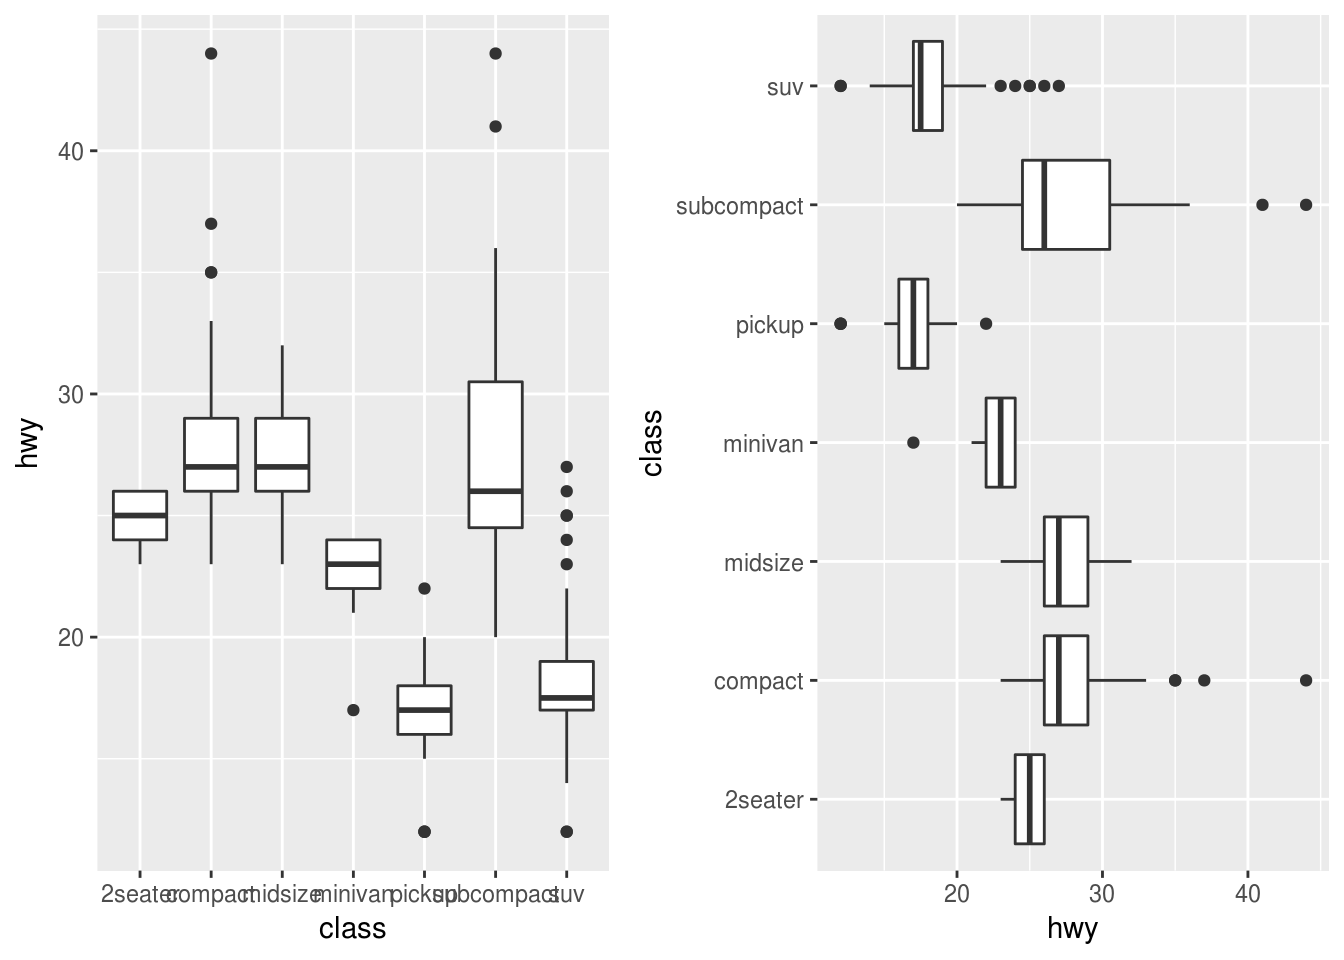
\includegraphics{Graficos_files/figure-latex/coord-flip-plot-1.pdf}

En el primer caso las etiquetas del eje x se superponen, pero en el
segundo es fácil verlas. No es la única forma de solucionar este
problema. También es posible cambiar el ángulo de las etiquetas para que
no se superpongan.

Otras veces es mejor reemplazar las coordenadas cartesianas por
coordenadas geográficas.

\begin{Shaded}
\begin{Highlighting}[]
\NormalTok{arg <-}\StringTok{ }\KeywordTok{map_data}\NormalTok{(}\StringTok{"world"}\NormalTok{, }\DataTypeTok{region =} \StringTok{"Argentina"}\NormalTok{)}

\KeywordTok{ggplot}\NormalTok{(}\DataTypeTok{data =}\NormalTok{ arg, }\DataTypeTok{mapping =} \KeywordTok{aes}\NormalTok{(}\DataTypeTok{x =}\NormalTok{ long, }\DataTypeTok{y =}\NormalTok{ lat, }\DataTypeTok{group =}\NormalTok{ group)) }\OperatorTok{+}
\StringTok{  }\KeywordTok{geom_polygon}\NormalTok{(}\DataTypeTok{fill =} \StringTok{"white"}\NormalTok{, }\DataTypeTok{color =} \StringTok{"black"}\NormalTok{)}

\KeywordTok{ggplot}\NormalTok{(}\DataTypeTok{data =}\NormalTok{ arg, }\DataTypeTok{mapping =} \KeywordTok{aes}\NormalTok{(}\DataTypeTok{x =}\NormalTok{ long, }\DataTypeTok{y =}\NormalTok{ lat, }\DataTypeTok{group =}\NormalTok{ group)) }\OperatorTok{+}
\StringTok{  }\KeywordTok{geom_polygon}\NormalTok{(}\DataTypeTok{fill =} \StringTok{"white"}\NormalTok{, }\DataTypeTok{color =} \StringTok{"black"}\NormalTok{)}
  \KeywordTok{coord_quickmap}\NormalTok{()}
\end{Highlighting}
\end{Shaded}

\begin{verbatim}
## 
## Attaching package: 'maps'
\end{verbatim}

\begin{verbatim}
## The following object is masked from 'package:purrr':
## 
##     map
\end{verbatim}

\begin{verbatim}
## <ggproto object: Class CoordQuickmap, CoordCartesian, Coord, gg>
##     aspect: function
##     default: FALSE
##     distance: function
##     expand: TRUE
##     is_linear: function
##     labels: function
##     limits: list
##     modify_scales: function
##     range: function
##     render_axis_h: function
##     render_axis_v: function
##     render_bg: function
##     render_fg: function
##     setup_data: function
##     setup_layout: function
##     setup_panel_params: function
##     setup_params: function
##     transform: function
##     super:  <ggproto object: Class CoordQuickmap, CoordCartesian, Coord, gg>
\end{verbatim}

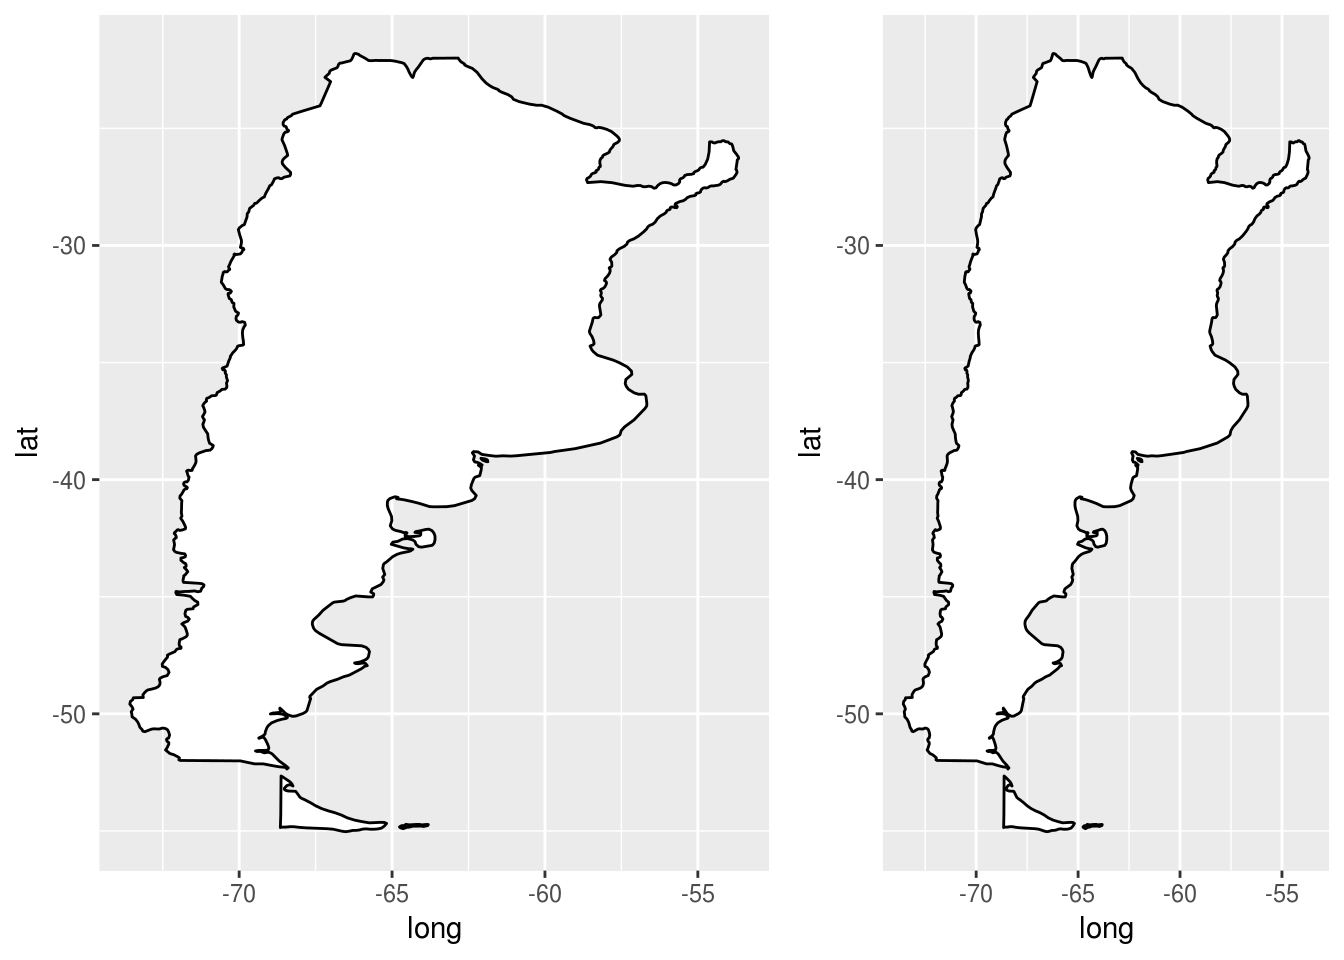
\includegraphics{Graficos_files/figure-latex/coord-quickmap-plot-1.pdf}

Esto evita que el mapa se deforme, ya que los grados de longitud no
miden lo mismo en todas las latitudes. Si van a hacer muchos mapas les
recomiendo que vean la extesión \texttt{ggmap} que tiene muchas
utilidades para hacer mejores mapas.

También existen la coordenadas polares. Un gráfico de torta, que les
recomiendo que no lo usen por los problemas de percepción que tiene, es
un gráfico de barras apiladas en coordernadas polares.

\begin{Shaded}
\begin{Highlighting}[]
\NormalTok{cxc <-}\StringTok{ }\KeywordTok{ggplot}\NormalTok{(mtcars, }\KeywordTok{aes}\NormalTok{(}\DataTypeTok{x =} \KeywordTok{factor}\NormalTok{(cyl))) }\OperatorTok{+}
\StringTok{  }\KeywordTok{geom_bar}\NormalTok{(}\DataTypeTok{width =} \DecValTok{1}\NormalTok{, }\DataTypeTok{colour =} \StringTok{"black"}\NormalTok{)}
\NormalTok{cxc }\OperatorTok{+}\StringTok{ }\KeywordTok{coord_polar}\NormalTok{()}
\end{Highlighting}
\end{Shaded}

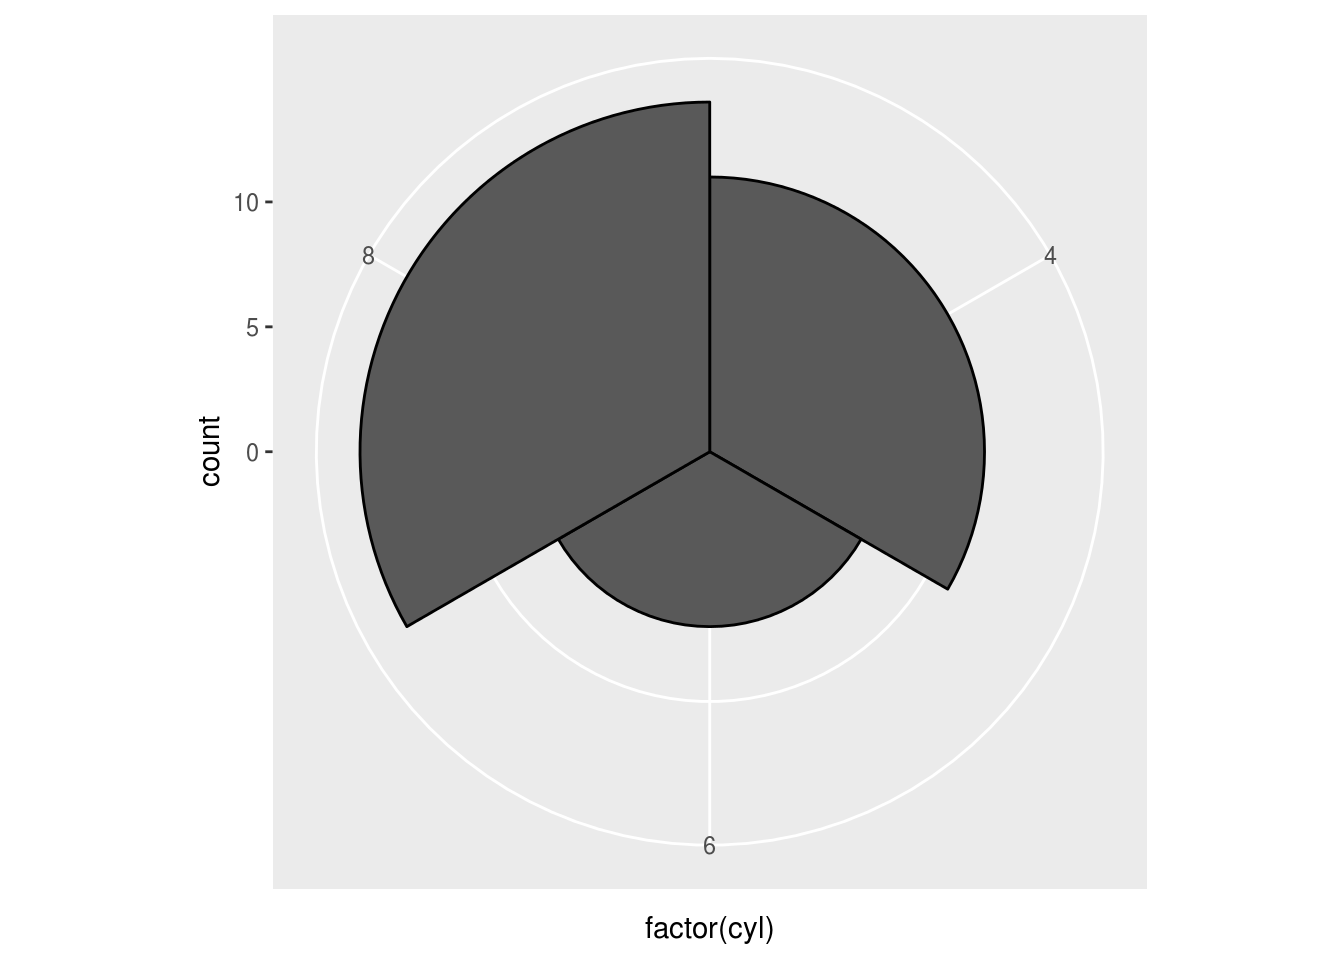
\includegraphics{Graficos_files/figure-latex/coord-polar-1.pdf}

\hypertarget{personalizando-el-grafico}{%
\section{Personalizando el gráfico}\label{personalizando-el-grafico}}

Hay varias maneras de personalizar los gráficos. Por un lado, las
estéticas pueden ser personalizadas cambiando las distintas
\texttt{scales} (escalas). Para cambiar el eje x se usa
\texttt{scale\_x\_*} donde * es el tipo de dato que tiene el eje: si es
númerico se usa \texttt{continuous} y si es categórico se usa
\texttt{discrete}. Se pueden cambiar muchas cosas: el título del eje
(\texttt{name}), el lugar de las marcas (\texttt{breaks}), las etiquetas
de las marcas (\texttt{labels}), y muchas más opciones.

\begin{Shaded}
\begin{Highlighting}[]
\KeywordTok{ggplot}\NormalTok{(}\DataTypeTok{data =}\NormalTok{ mpg) }\OperatorTok{+}
\StringTok{  }\KeywordTok{geom_point}\NormalTok{(}\DataTypeTok{mapping =} \KeywordTok{aes}\NormalTok{(}\DataTypeTok{x =}\NormalTok{ displ, }\DataTypeTok{y =}\NormalTok{ hwy))}\OperatorTok{+}
\StringTok{  }\KeywordTok{scale_x_continuous}\NormalTok{(}\DataTypeTok{name =} \StringTok{"Cilindrada (l)"}\NormalTok{, }\DataTypeTok{breaks =} \DecValTok{1}\OperatorTok{:}\DecValTok{7}\NormalTok{, }
                     \DataTypeTok{labels =} \KeywordTok{c}\NormalTok{(}\StringTok{"uno"}\NormalTok{, }\StringTok{"dos"}\NormalTok{, }\StringTok{"tres"}\NormalTok{, }\StringTok{"cuatro"}\NormalTok{, }\StringTok{"cinco"}\NormalTok{, }
                                \StringTok{"seis"}\NormalTok{, }\StringTok{"siete"}\NormalTok{))}
\end{Highlighting}
\end{Shaded}

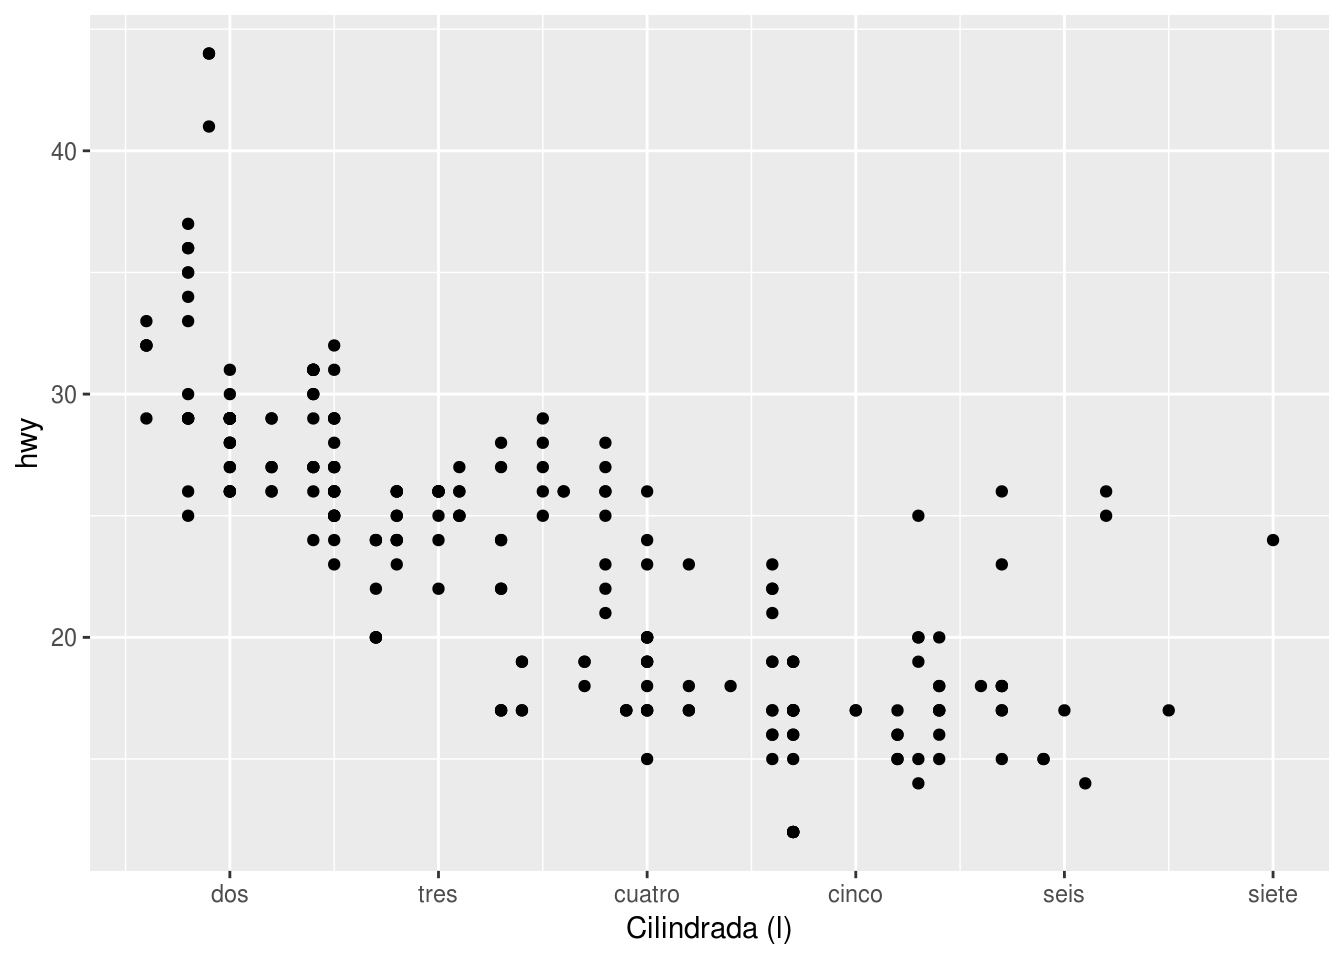
\includegraphics{Graficos_files/figure-latex/scale-1.pdf}

Un atajo para modificar los nombres de los ejes es usar la función
\texttt{labs()}, pero solo se pueden modificar los nombres de los ejes y
nada más.

\begin{Shaded}
\begin{Highlighting}[]
\KeywordTok{ggplot}\NormalTok{(}\DataTypeTok{data =}\NormalTok{ mpg) }\OperatorTok{+}
\StringTok{  }\KeywordTok{geom_point}\NormalTok{(}\DataTypeTok{mapping =} \KeywordTok{aes}\NormalTok{(}\DataTypeTok{x =}\NormalTok{ displ, }\DataTypeTok{y =}\NormalTok{ hwy))}\OperatorTok{+}
\StringTok{  }\KeywordTok{labs}\NormalTok{(}\DataTypeTok{x =} \StringTok{"Cilindrada (l)"}\NormalTok{, }\DataTypeTok{y =} \StringTok{"Millas por galón en Autopista"}\NormalTok{)}
\end{Highlighting}
\end{Shaded}

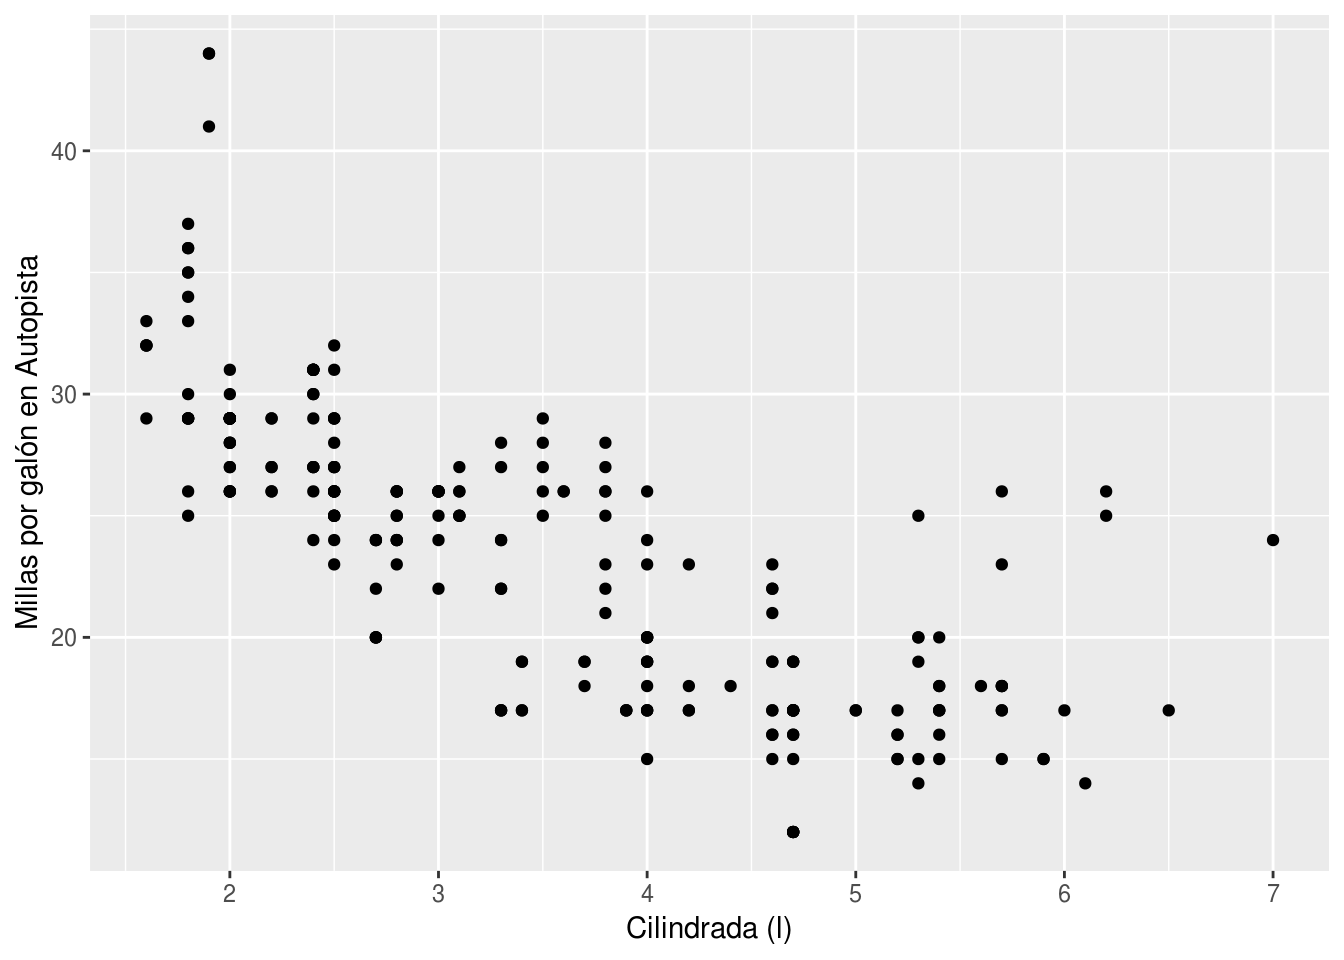
\includegraphics{Graficos_files/figure-latex/labs-1.pdf}

También se puede modificar los colores que se asignan.

\begin{Shaded}
\begin{Highlighting}[]
\KeywordTok{ggplot}\NormalTok{(}\DataTypeTok{data =}\NormalTok{ mpg) }\OperatorTok{+}
\StringTok{  }\KeywordTok{geom_point}\NormalTok{(}\DataTypeTok{mapping =} \KeywordTok{aes}\NormalTok{(}\DataTypeTok{x =}\NormalTok{ displ, }\DataTypeTok{y =}\NormalTok{ hwy, }\DataTypeTok{colour =}\NormalTok{ class))}\OperatorTok{+}\StringTok{ }
\StringTok{  }\KeywordTok{scale_color_brewer}\NormalTok{(}\StringTok{"Clase"}\NormalTok{)}

\KeywordTok{ggplot}\NormalTok{(}\DataTypeTok{data =}\NormalTok{ mpg) }\OperatorTok{+}
\StringTok{  }\KeywordTok{geom_point}\NormalTok{(}\DataTypeTok{mapping =} \KeywordTok{aes}\NormalTok{(}\DataTypeTok{x =}\NormalTok{ displ, }\DataTypeTok{y =}\NormalTok{ hwy, }\DataTypeTok{colour =}\NormalTok{ class))}\OperatorTok{+}\StringTok{ }
\StringTok{  }\KeywordTok{scale_color_brewer}\NormalTok{(}\StringTok{"Clase"}\NormalTok{, }\DataTypeTok{palette =} \StringTok{"RdYlBu"}\NormalTok{)}

\KeywordTok{ggplot}\NormalTok{(}\DataTypeTok{data =}\NormalTok{ mpg) }\OperatorTok{+}
\StringTok{  }\KeywordTok{geom_point}\NormalTok{(}\DataTypeTok{mapping =} \KeywordTok{aes}\NormalTok{(}\DataTypeTok{x =}\NormalTok{ displ, }\DataTypeTok{y =}\NormalTok{ hwy, }\DataTypeTok{colour =}\NormalTok{ class))}\OperatorTok{+}\StringTok{ }
\StringTok{  }\KeywordTok{scale_color_viridis_d}\NormalTok{(}\StringTok{"Clase"}\NormalTok{)}
\end{Highlighting}
\end{Shaded}

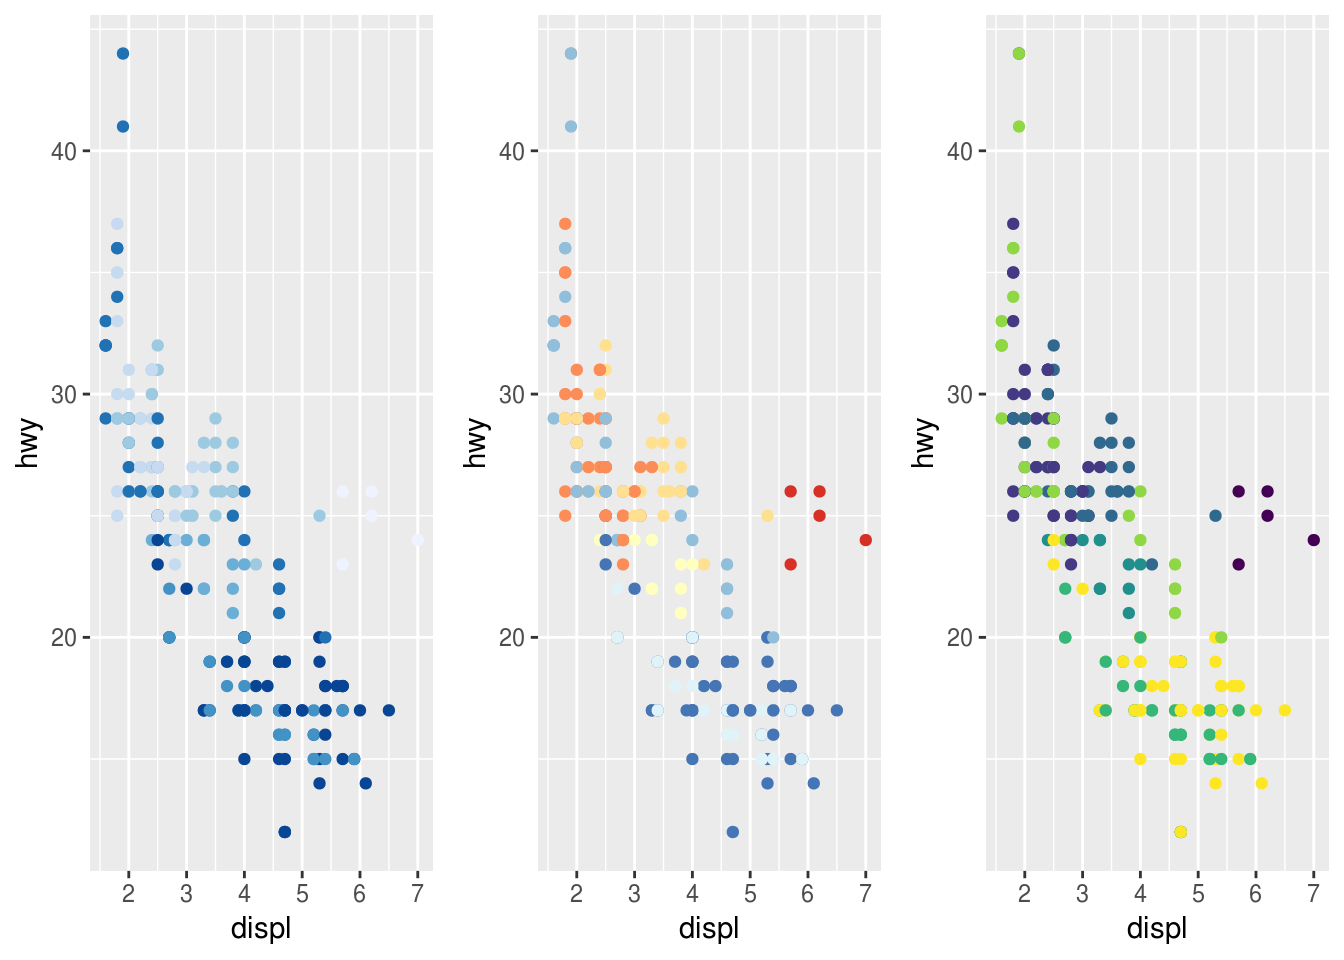
\includegraphics{Graficos_files/figure-latex/colores-plot-1.pdf}

Hay muchas más opciones disponibles, ya que como dice el dicho: ``Para
gustos, los colores''. Si quieren conocerlas te recomiendo que lean la
ayuda de cada una o visiten el sitio de ggplot2.

Vemos que hay patrón común con las escalas, todas empiezan por
\texttt{scale}, luego sigue por lo que se quiere modificar: el eje,
\texttt{x} o \texttt{y}; el color, \texttt{color}; relleno,
\texttt{fill}; la forma, \texttt{shape}; el tipo de línea
\texttt{linetype}, etc. Cada uno de las estéticas tiene su escale.
Luego, salvo alguna excepción, siguen por el tipo de dato o en el caso
de los colores por el método de creación del color. Vale la pena agregar
que cada escale tiene su versión manual para un control total de la
apariencia.

Por otro lado están los elementos del gráfico que modifican la
apariencia general del gráfico. El tipo y tamaño de letra, el color del
fondo, el grosor de la líneas de los ejes, la dirección de marcas, la
dirección del texto, y ¡todo lo demás!. Todo esto está unido a lo que es
el tema (\texttt{theme}) del gráfico. Se pueden guardar las
modificaciones para usarla facilmente y ya vienen algunas opciones en
\texttt{ggplot} y hay más en el paquete \texttt{ggthemes} y otros.

\begin{Shaded}
\begin{Highlighting}[]
\KeywordTok{ggplot}\NormalTok{(}\DataTypeTok{data =}\NormalTok{ mpg) }\OperatorTok{+}
\StringTok{  }\KeywordTok{geom_point}\NormalTok{(}\DataTypeTok{mapping =} \KeywordTok{aes}\NormalTok{(}\DataTypeTok{x =}\NormalTok{ displ, }\DataTypeTok{y =}\NormalTok{ hwy, }\DataTypeTok{colour =}\NormalTok{ class)) }\OperatorTok{+}
\StringTok{  }\KeywordTok{theme_classic}\NormalTok{()}
\end{Highlighting}
\end{Shaded}

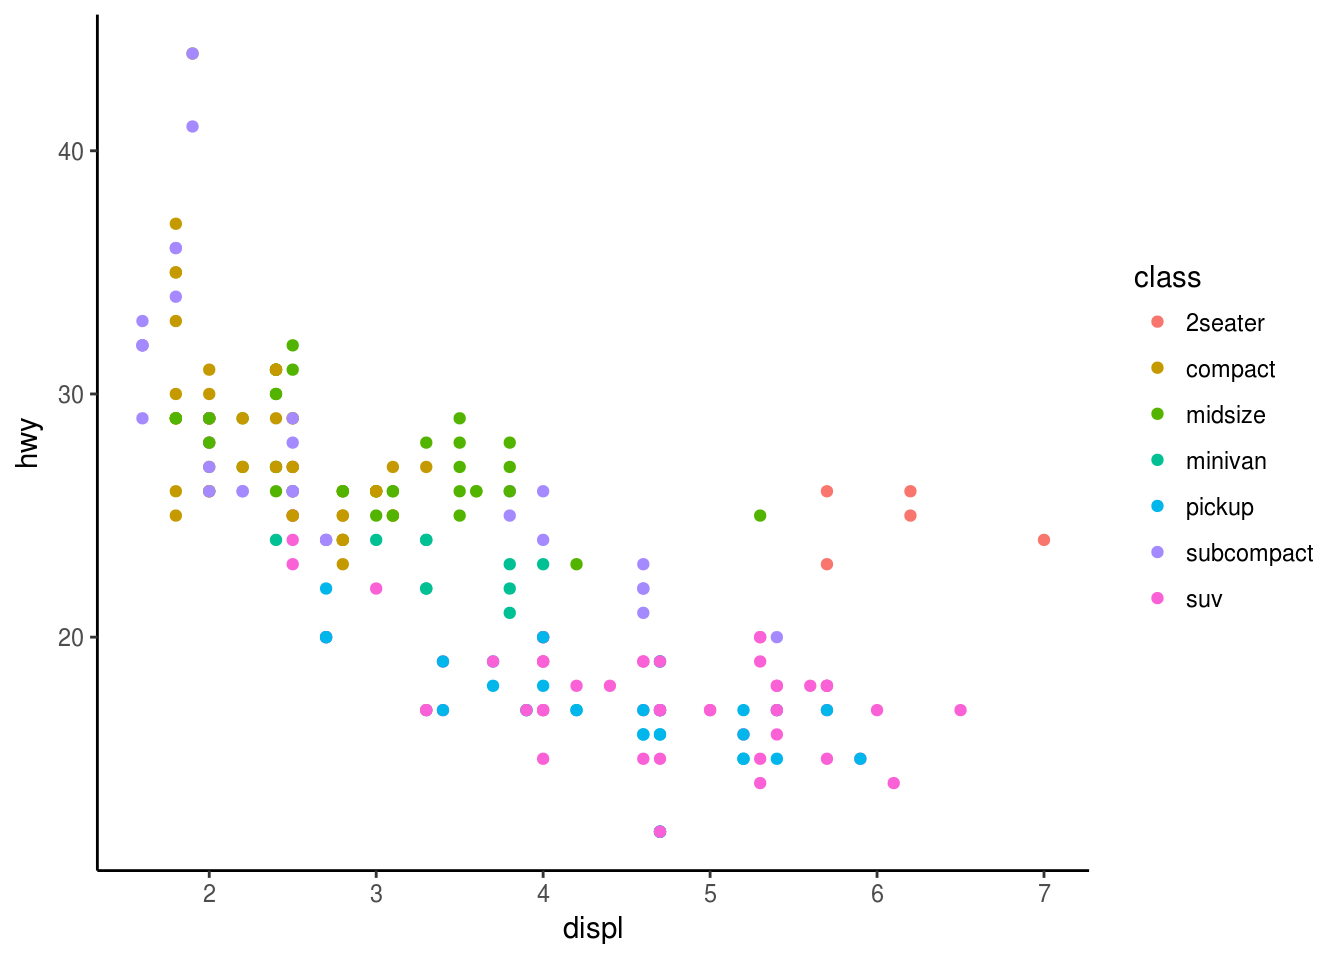
\includegraphics{Graficos_files/figure-latex/temas-1.pdf}

Para modificar algún elemento en particular usamos la función
\texttt{theme()} al final del gráfico. Dentro de la llamada a
\texttt{theme} modificamos el argumento que queremos cambiar usando la
función \texttt{element\_*()}.

\begin{Shaded}
\begin{Highlighting}[]
\KeywordTok{ggplot}\NormalTok{(}\DataTypeTok{data =}\NormalTok{ mpg) }\OperatorTok{+}
\StringTok{  }\KeywordTok{geom_bar}\NormalTok{(}\DataTypeTok{mapping =} \KeywordTok{aes}\NormalTok{(}\DataTypeTok{x =}\NormalTok{ class, }\DataTypeTok{fill =}\NormalTok{ fl)) }\OperatorTok{+}
\StringTok{  }\KeywordTok{theme}\NormalTok{(}\DataTypeTok{axis.text.x =} \KeywordTok{element_text}\NormalTok{(}\DataTypeTok{angle =} \DecValTok{45}\NormalTok{, }\DataTypeTok{hjust =} \DecValTok{1}\NormalTok{, }\DataTypeTok{vjust =} \DecValTok{1}\NormalTok{))}
\end{Highlighting}
\end{Shaded}

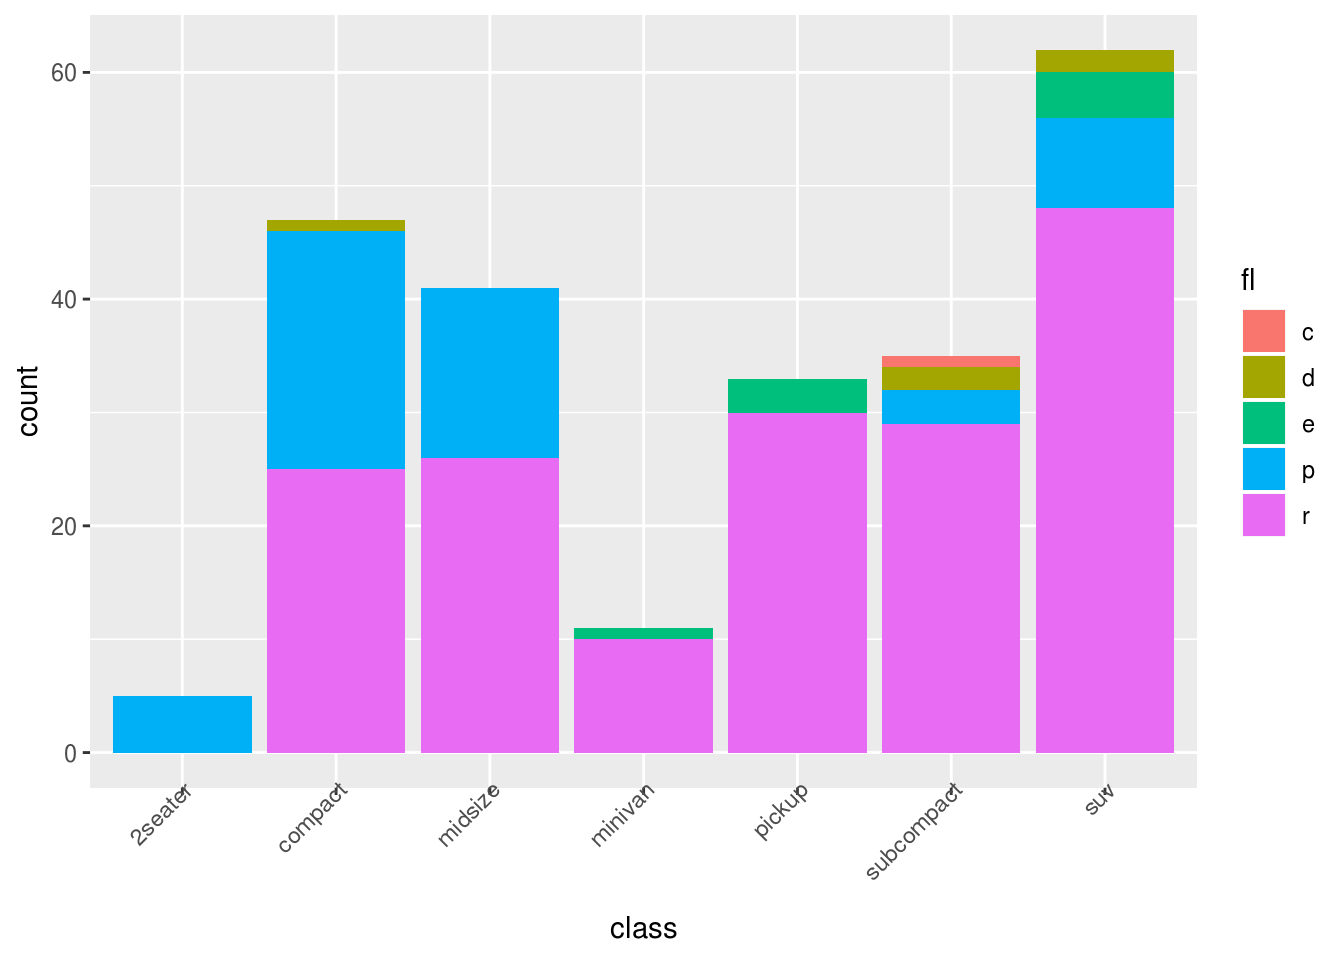
\includegraphics{Graficos_files/figure-latex/personalizar-temas-1.pdf}

Sí, es bastante complicado. Pero por suerte se puede guardar y
reutilizar.

\begin{Shaded}
\begin{Highlighting}[]
\NormalTok{x_}\DecValTok{45}\NormalTok{ <-}\StringTok{ }\KeywordTok{theme}\NormalTok{(}\DataTypeTok{axis.text.x =} \KeywordTok{element_text}\NormalTok{(}\DataTypeTok{angle =} \DecValTok{45}\NormalTok{, }\DataTypeTok{hjust =} \DecValTok{1}\NormalTok{, }\DataTypeTok{vjust =} \DecValTok{1}\NormalTok{))}

\KeywordTok{ggplot}\NormalTok{(}\DataTypeTok{data =}\NormalTok{ mpg) }\OperatorTok{+}
\StringTok{  }\KeywordTok{geom_bar}\NormalTok{(}\DataTypeTok{mapping =} \KeywordTok{aes}\NormalTok{(}\DataTypeTok{x =}\NormalTok{ class, }\DataTypeTok{fill =}\NormalTok{ fl)) }\OperatorTok{+}
\StringTok{  }\NormalTok{x_}\DecValTok{45}
\end{Highlighting}
\end{Shaded}

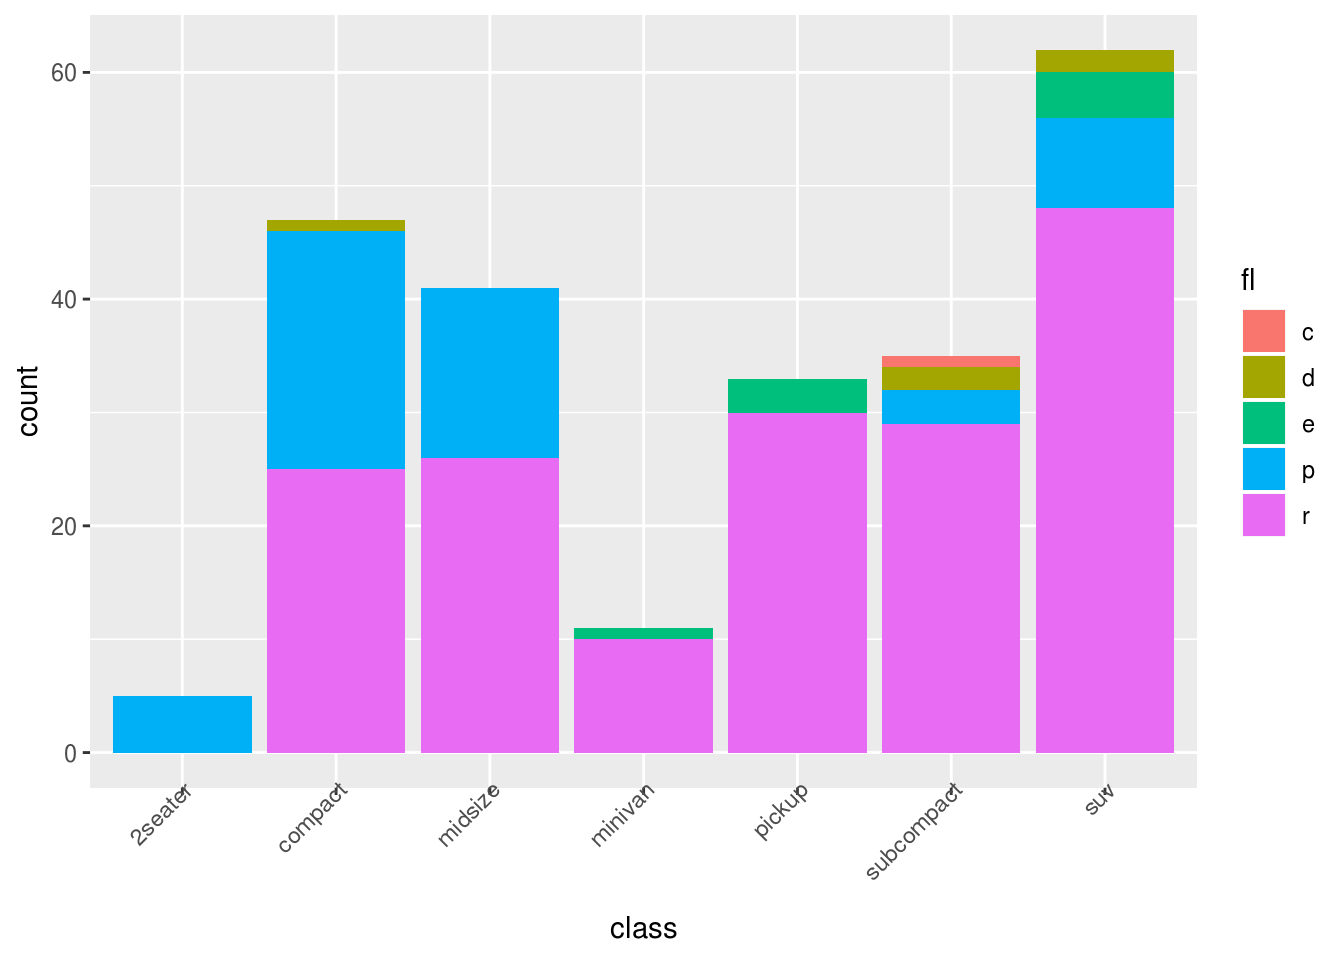
\includegraphics{Graficos_files/figure-latex/a-45-grados-1.pdf}

También es posible cambiar la posición de la leyenda o eliminarla
completamente.

\begin{Shaded}
\begin{Highlighting}[]
\KeywordTok{ggplot}\NormalTok{(}\DataTypeTok{data =}\NormalTok{ mpg) }\OperatorTok{+}
\StringTok{  }\KeywordTok{geom_bar}\NormalTok{(}\DataTypeTok{mapping =} \KeywordTok{aes}\NormalTok{(}\DataTypeTok{x =}\NormalTok{ class, }\DataTypeTok{fill =}\NormalTok{ fl)) }\OperatorTok{+}
\StringTok{  }\KeywordTok{theme}\NormalTok{(}\DataTypeTok{legend.position =} \StringTok{"bottom"}\NormalTok{)}

\KeywordTok{ggplot}\NormalTok{(}\DataTypeTok{data =}\NormalTok{ mpg) }\OperatorTok{+}
\StringTok{  }\KeywordTok{geom_bar}\NormalTok{(}\DataTypeTok{mapping =} \KeywordTok{aes}\NormalTok{(}\DataTypeTok{x =}\NormalTok{ class, }\DataTypeTok{fill =}\NormalTok{ fl)) }\OperatorTok{+}
\StringTok{  }\KeywordTok{theme}\NormalTok{(}\DataTypeTok{legend.position =} \StringTok{"none"}\NormalTok{)}
\end{Highlighting}
\end{Shaded}

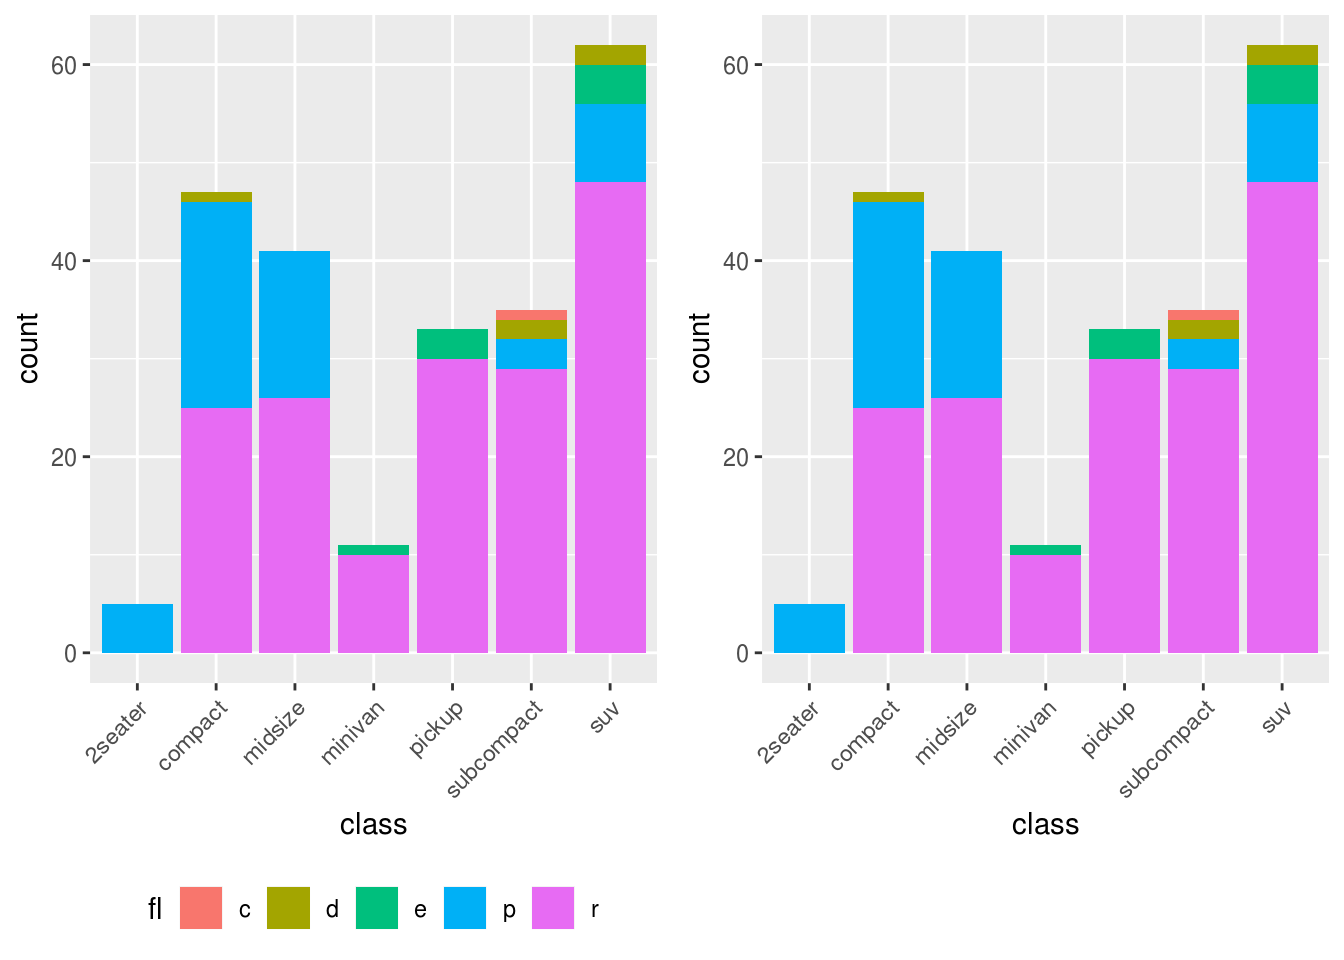
\includegraphics{Graficos_files/figure-latex/cambiar-leyenda-plot-1.pdf}

\hypertarget{manejo-de-datos}{%
\chapter{Manejo de datos}\label{manejo-de-datos}}

\begin{atencion}
Antes de comenzar bajen el archivo donde realizarán su informe
reproducible. En la consola copien este código:

\texttt{download.file(url\ =\ "git.io/informe-manejo",\ destfile\ =\ "informe-manejo-de-datos.Rmd")}

Pueden abrirlo desde la pestaña de archivos, a la derecha. Cambien el
nombre por el suyo en el encabezado y mientras leen este capítulo
respondan las preguntas.
\end{atencion}

Una parte muy importante del análisis de datos, es el manejo de ellos.
Como seleccionar columnas, filtrar datos, y realizar operaciones sobre
ellos. Vamos a usar el paquete \texttt{dplyr} y \texttt{tidyr} para el
manejo. Los paquetes extienden la funcionalidad de \emph{R} agregando
nuevas funciones.

\begin{Shaded}
\begin{Highlighting}[]
\KeywordTok{library}\NormalTok{(}\StringTok{"dplyr"}\NormalTok{)}

\NormalTok{nombres <-}\StringTok{ }\KeywordTok{readRDS}\NormalTok{(}\StringTok{"data/nombres-1980-1999.RDS"}\NormalTok{)}
\end{Highlighting}
\end{Shaded}

Revisemos el código. Con \texttt{library("dplyr")} cargamos el paquete
dplyr. Luego, leemos el archivo que contiene los datos y le asignamos el
nombre \texttt{nombres}. Si no le asignasemos ningún nombre, se leerían
los datos, imprimiendose en la consola y luego se borrarían de la
memoría.

Para revisar su contenido podemos escribir el nombre del objeto o usar
la función \texttt{glimpse}

\begin{Shaded}
\begin{Highlighting}[]
\KeywordTok{glimpse}\NormalTok{(nombres)}
\end{Highlighting}
\end{Shaded}

\BeginKnitrBlock{exercise}
\protect\hypertarget{exr:ejercicio-4}{}{\label{exr:ejercicio-4} }Escriban el
nombre del objeto o usen la función \texttt{glimpse} para ver que tiene
dentro el objeto \texttt{nombres}.

\begin{enumerate}
\def\labelenumi{\arabic{enumi}.}
\tightlist
\item
  ¿Cuantas columnas tiene y como se llaman?
\item
  ¿Que tipo de dato tiene cada columna?
\end{enumerate}
\EndKnitrBlock{exercise}

En \emph{R} existen diversos tipos de dato, en estos datos solo hay 2:
entero (\texttt{integer}) y carácter (\texttt{character}). El primero
son números enteros y el segundo es texto. Con el primero se puede hacer
operaciones matemáticas y con el segundo otro tipo de operaciones, pero
no matemáticas. Es importante comprobar que los tipos de datos se
correspondan con lo que esperamos. Si no los resultados pueden no ser
los correctos o dar errores. Por ejemplo, el tipo de dato númerico puede
ser leído como \texttt{chr} y no podremos calcular la media.

\hypertarget{seleccionando-datos}{%
\section{Seleccionando datos}\label{seleccionando-datos}}

Muchas veces solo nos interesa un subconjunto de datos. Una forma de
seleccionar datos es usando la función \texttt{filter()}.

\begin{Shaded}
\begin{Highlighting}[]
\NormalTok{nombres }\OperatorTok\StringTok{ }
\StringTok{  }\KeywordTok{filter}\NormalTok{(nombre }\OperatorTok{==}\StringTok{ "Luciano"}\NormalTok{) }\OperatorTok\StringTok{ }
\StringTok{  }\KeywordTok{filter}\NormalTok{(anio }\OperatorTok{==}\StringTok{ }\DecValTok{1984}\NormalTok{)}
\end{Highlighting}
\end{Shaded}

Acá empezamos a ver varias cosas nuevas. Primero tenemos el símbolo
\texttt{\%\textgreater{}\%} conocido en inglés como \emph{pipe}, la
traducción más correcta al español es tubo. Lo que hace este símbolo es
enviar la salida de la operación a la izquierda a la función de la
derecha. Prueben poner cada comando en orden y ver cual es la salida.
Esto es:

\begin{Shaded}
\begin{Highlighting}[]
\NormalTok{nombres}
\end{Highlighting}
\end{Shaded}

Luego,

\begin{Shaded}
\begin{Highlighting}[]
\NormalTok{nombres }\OperatorTok\StringTok{ }
\StringTok{  }\KeywordTok{filter}\NormalTok{(nombre }\OperatorTok{==}\StringTok{ "Luciano"}\NormalTok{)}
\end{Highlighting}
\end{Shaded}

La función \texttt{filter()} filtra un conjunto de datos según los
valores de la columna/s que seleccionemos cuyos valores sean igual a
\texttt{Luciano} en este caso. Y luego filtramos la columna
\texttt{anio} solo los años que sean iguales a 1984.

\BeginKnitrBlock{exercise}
\protect\hypertarget{exr:ejercicio-5}{}{\label{exr:ejercicio-5} }Prueben
cambiar el nombre por el suyo y el año por su año de nacimiento.
\EndKnitrBlock{exercise}

El operador que usamos para la igualdad es \texttt{==}. Este operador,
de igualdad, es parte de la familia de operadores lógicos, o booleanos
en terminología de ciencias de la información. Son lógicos porque van a
comparar valores y dar como resultado \textbf{verdadero} (\texttt{TRUE})
o \textbf{falso} (\texttt{FALSE}). En la Tabla \ref{tab:tabla-logicos}
podemos ver la lista de operadores lógicos.

\begin{table}

\caption{\label{tab:tabla-logicos}Operadores Lógicos en R.}
\centering
\begin{tabular}[t]{l|l}
\hline
Operador & Descripción\\
\hline
< & menor que\\
\hline
<= & menor o igual que\\
\hline
> & mayor que\\
\hline
>= & mayor o igual que\\
\hline
== & exactamente igual a\\
\hline
!= & no igual a\\
\hline
!x & no x\\
\hline
x | y & x *O* y\\
\hline
x \& y & x *E* y\\
\hline
isTRUE(x) & comprueba si x es verdadero\\
\hline
\end{tabular}
\end{table}

Los primeros cinco son bastante sencillos y los han estado usando desde
la primaria. Así que vamos a explicar en más profundidad los otros. El
símbolo \texttt{!=} va a devolver \texttt{TRUE} cuando los valores sean
diferentes al que pusimos. Por ejemplo:

\begin{Shaded}
\begin{Highlighting}[]
\CommentTok{# x una secuencia de 1 a 10}
\NormalTok{x <-}\StringTok{ }\DecValTok{1}\OperatorTok{:}\DecValTok{10}
\CommentTok{# Todos los valores distintos a 5}
\NormalTok{x }\OperatorTok{!=}\StringTok{ }\DecValTok{5}
\end{Highlighting}
\end{Shaded}

\begin{verbatim}
##  [1]  TRUE  TRUE  TRUE  TRUE FALSE  TRUE  TRUE  TRUE  TRUE  TRUE
\end{verbatim}

\BeginKnitrBlock{exercise}[Nombres comunes]
\protect\hypertarget{exr:nombre-comun}{}{\label{exr:nombre-comun}
\iffalse (Nombres comunes) \fi{} }¿Cómo filtrarían los nombres raros
excluyéndolos del conjunto de datos?

Guarden el resultado como nombres\_comunes y calculen el total por
nombre.

Nota: Por coherencia, definamos nombres raros como los que son menos de
100.
\EndKnitrBlock{exercise}

Otro operador muy útil es el de negación \texttt{!} que invierte las
comparaciones, convierte los falsos en verdaderos y los verdaderos en
falsos. Siguiendo nuestro ejemplo:

\begin{Shaded}
\begin{Highlighting}[]
\OperatorTok{!}\NormalTok{x }\OperatorTok{!=}\StringTok{ }\DecValTok{5}
\end{Highlighting}
\end{Shaded}

\begin{verbatim}
##  [1] FALSE FALSE FALSE FALSE  TRUE FALSE FALSE FALSE FALSE FALSE
\end{verbatim}

Es un ejemplo trivial, que podría haber sido resuelto más sencillamente
usando \texttt{==}. Pero es muy útil cuando queremos seleccionar todos
los datos que no cumplan un conjuto de condiciones. Lo que nos lleva al
operador \texttt{\textbar{}} (\emph{O}) y el operador \texttt{\&}
(\emph{Y}). El primero va a devolver verdadero cuando \emph{al menos
uno} de los valores sea verdadero. Por ejemplo:

\begin{Shaded}
\begin{Highlighting}[]
\OtherTok{TRUE} \OperatorTok{|}\StringTok{ }\OtherTok{TRUE}
\end{Highlighting}
\end{Shaded}

\begin{verbatim}
## [1] TRUE
\end{verbatim}

\begin{Shaded}
\begin{Highlighting}[]
\OtherTok{TRUE} \OperatorTok{|}\StringTok{ }\OtherTok{FALSE}
\end{Highlighting}
\end{Shaded}

\begin{verbatim}
## [1] TRUE
\end{verbatim}

\begin{Shaded}
\begin{Highlighting}[]
\OtherTok{FALSE} \OperatorTok{|}\StringTok{ }\OtherTok{TRUE}
\end{Highlighting}
\end{Shaded}

\begin{verbatim}
## [1] TRUE
\end{verbatim}

\begin{Shaded}
\begin{Highlighting}[]
\OtherTok{FALSE} \OperatorTok{|}\StringTok{ }\OtherTok{FALSE}
\end{Highlighting}
\end{Shaded}

\begin{verbatim}
## [1] FALSE
\end{verbatim}

Por otro lado, el operador lógico \emph{Y} \texttt{\&} solo devuelve
verdadero cuando \emph{ambos valores} son verdaderos.

\begin{Shaded}
\begin{Highlighting}[]
\OtherTok{TRUE} \OperatorTok{&}\StringTok{ }\OtherTok{TRUE}
\end{Highlighting}
\end{Shaded}

\begin{verbatim}
## [1] TRUE
\end{verbatim}

\begin{Shaded}
\begin{Highlighting}[]
\OtherTok{TRUE} \OperatorTok{&}\StringTok{ }\OtherTok{FALSE}
\end{Highlighting}
\end{Shaded}

\begin{verbatim}
## [1] FALSE
\end{verbatim}

\begin{Shaded}
\begin{Highlighting}[]
\OtherTok{FALSE} \OperatorTok{&}\StringTok{ }\OtherTok{TRUE}
\end{Highlighting}
\end{Shaded}

\begin{verbatim}
## [1] FALSE
\end{verbatim}

\begin{Shaded}
\begin{Highlighting}[]
\OtherTok{FALSE} \OperatorTok{&}\StringTok{ }\OtherTok{FALSE}
\end{Highlighting}
\end{Shaded}

\begin{verbatim}
## [1] FALSE
\end{verbatim}

Los operadores se evalúan en el orden que aparecen a menos que haya
paréntesis, entonces se evalúa primero dentro del paréntesis y luego
fuera.

\BeginKnitrBlock{exercise}
\protect\hypertarget{exr:ejercicio-6}{}{\label{exr:ejercicio-6} }¿Qué
resultado darán las siguientes evaluaciones? Piensen que resultado
tendría que dar y luego comprueben lo que piensan con lo que les
devuelve R.

\begin{enumerate}
\def\labelenumi{\arabic{enumi}.}
\tightlist
\item
  TRUE \textbar{} FALSE \textbar{} TRUE
\item
  TRUE \textbar{} FALSE \& TRUE
\item
  TRUE \textbar{} (FALSE \& TRUE)
\item
  TRUE != FALSE \& TRUE
\item
  !(TRUE \textbar{} FALSE) \& TRUE
\end{enumerate}
\EndKnitrBlock{exercise}

Estos dos últimos operadores son muy importantes porque nos permiten
comprobar distintas condiciones. Por ejemplo, no hay un operador para
seleccionar todos los valores entre \emph{a} y \emph{b} (siendo \emph{a}
y \emph{b} dos números cualesquiera). Podemos hacerlo combinando por un
lado, x \textgreater{} a y x \textless{} b ¿Y cómo debemos combinar
estas dos comparaciones? ¿Usando el operador \texttt{\&} o el
\texttt{\textbar{}}? Queremos los valores que cumplen con ambas
condiciones, que sean mayores que a y menores que b, por lo tanto
debemos usar el operador \texttt{\&}.

\begin{Shaded}
\begin{Highlighting}[]
\CommentTok{# Si a = 3 y b = 6}
\NormalTok{( x }\OperatorTok{>}\StringTok{ }\DecValTok{3}\NormalTok{ ) }\OperatorTok{&}\StringTok{ }\NormalTok{( x }\OperatorTok{<}\StringTok{ }\DecValTok{6}\NormalTok{)}
\end{Highlighting}
\end{Shaded}

\begin{verbatim}
##  [1] FALSE FALSE FALSE  TRUE  TRUE FALSE FALSE FALSE FALSE FALSE
\end{verbatim}

Estos valores corresponden a la posición de los valores que cumplen o no
con la condición. Usando corchetes \texttt{{[}{]}} podemos seleccionar
solo los verdaderos

\begin{Shaded}
\begin{Highlighting}[]
\NormalTok{x[( x }\OperatorTok{>}\StringTok{ }\DecValTok{3}\NormalTok{ ) }\OperatorTok{&}\StringTok{ }\NormalTok{( x }\OperatorTok{<}\StringTok{ }\DecValTok{6}\NormalTok{)]}
\end{Highlighting}
\end{Shaded}

\begin{verbatim}
## [1] 4 5
\end{verbatim}

La función \texttt{filter()} hace algo similar para conjuntos de datos
(\texttt{data.frames} o \texttt{tibbles}).

\BeginKnitrBlock{exercise}
\protect\hypertarget{exr:ejercicio-7}{}{\label{exr:ejercicio-7}
}Anteriormente usamos dos operaciones de \texttt{filter()} para
seleccionar el nombre y el año. Pero es posible usar solo una con los
operadores lógicos que vimos. Intenten hacerlo.
\EndKnitrBlock{exercise}

Finalmente está \texttt{isTRUE()} que devuelve \texttt{TRUE} cuando el
objeto es \texttt{TRUE} lo que suena bastante obvio. Pero es parte de
una familia que permite comprobar si un objeto es del tipo esperado. Por
ejempo: \texttt{is.numeric()} comprueba que el objeto es un vector con
algún tipo de número.

Otra forma de seleccionar datos es por posición. Es decir, seleccionar
los primeras diez filas:

\begin{Shaded}
\begin{Highlighting}[]
\NormalTok{nombres_comunes }\OperatorTok\StringTok{ }
\StringTok{  }\KeywordTok{slice}\NormalTok{(}\DecValTok{1}\OperatorTok{:}\DecValTok{10}\NormalTok{)}
\end{Highlighting}
\end{Shaded}

\begin{verbatim}
## # A tibble: 10 x 3
##    nombre          anio cantidad
##    <chr>          <int>    <int>
##  1 Aaron           2012      152
##  2 Aaron           2013      167
##  3 Aaron           2014      200
##  4 Aaron Benjamin  2012      108
##  5 Aaron Benjamin  2013      120
##  6 Aaron Benjamin  2014      125
##  7 Abel            1982      102
##  8 Abel            1989      103
##  9 Abel            1990      102
## 10 Abigail         1991      132
\end{verbatim}

O seleccionar las primeras 10 filas que corresponden números primos:

\begin{Shaded}
\begin{Highlighting}[]
\NormalTok{nombres_comunes }\OperatorTok\StringTok{ }
\StringTok{  }\KeywordTok{slice}\NormalTok{(}\KeywordTok{c}\NormalTok{(}\DecValTok{2}\NormalTok{, }\DecValTok{3}\NormalTok{, }\DecValTok{5}\NormalTok{, }\DecValTok{7}\NormalTok{, }\DecValTok{11}\NormalTok{, }\DecValTok{13}\NormalTok{, }\DecValTok{17}\NormalTok{, }\DecValTok{19}\NormalTok{, }\DecValTok{23}\NormalTok{, }\DecValTok{29}\NormalTok{))}
\end{Highlighting}
\end{Shaded}

\begin{verbatim}
## # A tibble: 10 x 3
##    nombre          anio cantidad
##    <chr>          <int>    <int>
##  1 Aaron           2013      167
##  2 Aaron           2014      200
##  3 Aaron Benjamin  2013      120
##  4 Abel            1982      102
##  5 Abigail         1992      120
##  6 Abigail         1994      198
##  7 Abigail         1998      210
##  8 Abigail         2010      171
##  9 Abigail         2014      278
## 10 Abril           1999      813
\end{verbatim}

También es posible eliminar las filas según posición:

\begin{Shaded}
\begin{Highlighting}[]
\NormalTok{nombres_comunes }\OperatorTok\StringTok{ }
\StringTok{  }\KeywordTok{slice}\NormalTok{(}\OperatorTok{-}\NormalTok{(}\DecValTok{1}\OperatorTok{:}\DecValTok{10}\NormalTok{)) }\CommentTok{#Tengan en cuenta los parentesis extra}
\end{Highlighting}
\end{Shaded}

\begin{verbatim}
## # A tibble: 33,665 x 3
##    nombre   anio cantidad
##    <chr>   <int>    <int>
##  1 Abigail  1992      120
##  2 Abigail  1993      165
##  3 Abigail  1994      198
##  4 Abigail  1995      182
##  5 Abigail  1996      159
##  6 Abigail  1997      167
##  7 Abigail  1998      210
##  8 Abigail  1999      174
##  9 Abigail  2010      171
## 10 Abigail  2011      152
## # ... with 33,655 more rows
\end{verbatim}

\BeginKnitrBlock{exercise}
\protect\hypertarget{exr:ejercicio-9}{}{\label{exr:ejercicio-9} } 1. ¿Qué
sucede si olvidan los paréntesis en el código de arriba? 2. Seleccionen
las últimas 10 filas.
\EndKnitrBlock{exercise}

\hypertarget{seleccionando-columnas}{%
\section{Seleccionando columnas}\label{seleccionando-columnas}}

La función para seleccionar columnas es \texttt{seletc()}. Hay muchas
formas de seleccionar columnas. La más obvia es por nombre de la
columna:

\begin{Shaded}
\begin{Highlighting}[]
\NormalTok{nombres_comunes }\OperatorTok\StringTok{ }
\StringTok{  }\KeywordTok{select}\NormalTok{(nombre, cantidad)}
\end{Highlighting}
\end{Shaded}

\begin{verbatim}
## # A tibble: 33,675 x 2
##    nombre         cantidad
##    <chr>             <int>
##  1 Aaron               152
##  2 Aaron               167
##  3 Aaron               200
##  4 Aaron Benjamin      108
##  5 Aaron Benjamin      120
##  6 Aaron Benjamin      125
##  7 Abel                102
##  8 Abel                103
##  9 Abel                102
## 10 Abigail             132
## # ... with 33,665 more rows
\end{verbatim}

También es posible seleccionar varias columnas usando secuencias:

\begin{Shaded}
\begin{Highlighting}[]
\NormalTok{nombres_comunes }\OperatorTok\StringTok{ }
\StringTok{  }\KeywordTok{select}\NormalTok{(nombre}\OperatorTok{:}\NormalTok{cantidad)}
\end{Highlighting}
\end{Shaded}

\begin{verbatim}
## # A tibble: 33,675 x 3
##    nombre          anio cantidad
##    <chr>          <int>    <int>
##  1 Aaron           2012      152
##  2 Aaron           2013      167
##  3 Aaron           2014      200
##  4 Aaron Benjamin  2012      108
##  5 Aaron Benjamin  2013      120
##  6 Aaron Benjamin  2014      125
##  7 Abel            1982      102
##  8 Abel            1989      103
##  9 Abel            1990      102
## 10 Abigail         1991      132
## # ... with 33,665 more rows
\end{verbatim}

De la misma forma se puede eliminar columnas usando el signo \texttt{-}.

\begin{Shaded}
\begin{Highlighting}[]
\NormalTok{ nombres_comunes }\OperatorTok\StringTok{ }
\StringTok{  }\KeywordTok{select}\NormalTok{(}\OperatorTok{-}\NormalTok{anio)}
\end{Highlighting}
\end{Shaded}

\begin{verbatim}
## # A tibble: 33,675 x 2
##    nombre         cantidad
##    <chr>             <int>
##  1 Aaron               152
##  2 Aaron               167
##  3 Aaron               200
##  4 Aaron Benjamin      108
##  5 Aaron Benjamin      120
##  6 Aaron Benjamin      125
##  7 Abel                102
##  8 Abel                103
##  9 Abel                102
## 10 Abigail             132
## # ... with 33,665 more rows
\end{verbatim}

Se pueden renombrar columnas

\begin{Shaded}
\begin{Highlighting}[]
\NormalTok{nombres_comunes }\OperatorTok\StringTok{ }
\StringTok{  }\KeywordTok{select}\NormalTok{(añ}\DataTypeTok{o =}\NormalTok{ anio)}
\end{Highlighting}
\end{Shaded}

\begin{verbatim}
## # A tibble: 33,675 x 1
##      año
##    <int>
##  1  2012
##  2  2013
##  3  2014
##  4  2012
##  5  2013
##  6  2014
##  7  1982
##  8  1989
##  9  1990
## 10  1991
## # ... with 33,665 more rows
\end{verbatim}

Pero se eliminan las no seleccionadas. Se puede renombrar sin tener que
seleccionar el resto usando la función \texttt{rename}

\begin{Shaded}
\begin{Highlighting}[]
\NormalTok{nombres_comunes }\OperatorTok\StringTok{ }
\StringTok{  }\KeywordTok{select}\NormalTok{(añ}\DataTypeTok{o =}\NormalTok{ anio)}
\end{Highlighting}
\end{Shaded}

\begin{verbatim}
## # A tibble: 33,675 x 1
##      año
##    <int>
##  1  2012
##  2  2013
##  3  2014
##  4  2012
##  5  2013
##  6  2014
##  7  1982
##  8  1989
##  9  1990
## 10  1991
## # ... with 33,665 more rows
\end{verbatim}

Hay muchas más formas de seleccionar columnas, pueden referirse a la
ayuda \texttt{?select}, \texttt{?select\_at} y también a este excelente
{[}tutorial{]}{[}\url{https://suzan.rbind.io/2018/01/dplyr-tutorial-1/}{]}
(en inglés).

\hypertarget{agregando-columnas}{%
\section{Agregando columnas}\label{agregando-columnas}}

Otra operación muy común es agregar nuevas columnas o variables. Por
ejemplo al transformar los datos es siempre \textbf{mala idea}
sobreescribir los datos originales.

Para esta operación sirve la función \texttt{mutate()}. Dado un
\emph{data frame} computa una valor para cada fila. Por ejemplo:

\begin{Shaded}
\begin{Highlighting}[]
\NormalTok{nombres }\OperatorTok\StringTok{ }
\StringTok{  }\KeywordTok{mutate}\NormalTok{(}\DataTypeTok{log_cantidad =} \KeywordTok{log10}\NormalTok{(cantidad))}
\end{Highlighting}
\end{Shaded}

\begin{verbatim}
## # A tibble: 3,749,133 x 4
##    nombre         anio cantidad log_cantidad
##    <chr>         <int>    <int>        <dbl>
##  1 A Aron Misael  2012        2        0.301
##  2 A Mi           1984        1        0.   
##  3 A N A          2012        1        0.   
##  4 A Reum         1983        5        0.699
##  5 A Reum         1987        7        0.845
##  6 A Sang         1994        4        0.602
##  7 Aaaraon        2013        1        0.   
##  8 Aadil          1992        1        0.   
##  9 Aage Andres    1990        1        0.   
## 10 Aage Carlos    1985        1        0.   
## # ... with 3,749,123 more rows
\end{verbatim}

Cualquier operación que funcione con vectores funciona con
\texttt{mutate()}. También funciona se pueden modificar columnas si el
nombre que asignamos ya está usado dentro de nuestro \emph{data frame}.

\hypertarget{operaciones-por-grupos}{%
\section{Operaciones por grupos}\label{operaciones-por-grupos}}

Muchas veces van a necesitar calcular por grupos: la suma, media,
varianza, etc. Por ejemplo, calcular el número total de personas con
cada nombre. Podrían hacerlo de esta forma:

\begin{Shaded}
\begin{Highlighting}[]
\NormalTok{nombres_comunes }\OperatorTok\StringTok{ }
\StringTok{  }\KeywordTok{filter}\NormalTok{(nombre }\OperatorTok{==}\StringTok{ "Luciano"}\NormalTok{) }\OperatorTok\StringTok{ }
\StringTok{  }\KeywordTok{summarise}\NormalTok{(}\DataTypeTok{total =} \KeywordTok{sum}\NormalTok{(cantidad))}
\end{Highlighting}
\end{Shaded}

\begin{verbatim}
## # A tibble: 1 x 1
##   total
##   <int>
## 1 13244
\end{verbatim}

Y repetirlo cambiando el nombre para cada uno de los nombres. Por su
puesto, esta forma de hacer las cosas es muy incómoda y propensa a
errores. Hay una forma más fácil y es usando \texttt{group\_by()}. Un
ejemplo:

\begin{Shaded}
\begin{Highlighting}[]
\CommentTok{# No intenten hacerlo en sus computadoras}
\CommentTok{# Los datos tienen más de 3 millones de registros y va a tomar un tiempo}
\NormalTok{nombres_comunes }\OperatorTok\StringTok{ }
\StringTok{  }\KeywordTok{group_by}\NormalTok{(nombre) }\OperatorTok\StringTok{ }
\StringTok{  }\KeywordTok{summarise}\NormalTok{(}\DataTypeTok{total =} \KeywordTok{sum}\NormalTok{(cantidad))}
\end{Highlighting}
\end{Shaded}

\begin{verbatim}
## # A tibble: 4,272 x 2
##    nombre           total
##    <chr>            <int>
##  1 Aaron              519
##  2 Aaron Benjamin     353
##  3 Abel               307
##  4 Abigail           2656
##  5 Abril             4163
##  6 Adolfo             688
##  7 Adrian            4186
##  8 Adrian Alberto    2009
##  9 Adrian Alejandro  3460
## 10 Adrian Eduardo     106
## # ... with 4,262 more rows
\end{verbatim}

Como pueden ver estos datos distan bastante de estar limpios ya que hay
muchos errores de entrada de datos, como nombres todo en mayúsculas,
versiones del mismo nombre con tilde y sin tilde, etc. Para evitar todo
ese ``ruido'', podríamos filtrar los nombres raros que son mayoría de
las entradas.

Además de usar la función \texttt{summarise()} se puede usar la función
\texttt{mutate} que va a hacer que queden la misma cantidad de casos.
Por ejemplo, calcular el número acumulado de personas con el mismo
nombre en a través de los años:

\begin{Shaded}
\begin{Highlighting}[]
\NormalTok{nombres_comunes }\OperatorTok\StringTok{ }
\StringTok{  }\KeywordTok{group_by}\NormalTok{(nombre) }\OperatorTok\StringTok{ }
\StringTok{  }\KeywordTok{arrange}\NormalTok{(anio, }\DataTypeTok{.by_group =} \OtherTok{TRUE}\NormalTok{) }\OperatorTok\StringTok{ }
\StringTok{  }\KeywordTok{mutate}\NormalTok{(}\DataTypeTok{acumulado =} \KeywordTok{cumsum}\NormalTok{(cantidad))}
\end{Highlighting}
\end{Shaded}

\begin{verbatim}
## # A tibble: 33,675 x 4
## # Groups:   nombre [4,272]
##    nombre          anio cantidad acumulado
##    <chr>          <int>    <int>     <int>
##  1 Aaron           2012      152       152
##  2 Aaron           2013      167       319
##  3 Aaron           2014      200       519
##  4 Aaron Benjamin  2012      108       108
##  5 Aaron Benjamin  2013      120       228
##  6 Aaron Benjamin  2014      125       353
##  7 Abel            1982      102       102
##  8 Abel            1989      103       205
##  9 Abel            1990      102       307
## 10 Abigail         1991      132       132
## # ... with 33,665 more rows
\end{verbatim}

Acá hay una función nueva, \texttt{arrange()}. Lo que hace. Esta función
ordena de manera creciente (0-9, a-z) un conjunto de datos. Por ejemplo:

\begin{Shaded}
\begin{Highlighting}[]
\NormalTok{nombres_comunes }\OperatorTok\StringTok{ }
\StringTok{  }\KeywordTok{arrange}\NormalTok{(cantidad)}
\end{Highlighting}
\end{Shaded}

\begin{verbatim}
## # A tibble: 33,675 x 3
##    nombre              anio cantidad
##    <chr>              <int>    <int>
##  1 Adolfo              1981      101
##  2 Adrian Alberto      1990      101
##  3 Adrian Maximiliano  1988      101
##  4 Agustin Adrian      1998      101
##  5 Agustina Alejandra  1997      101
##  6 Ailin               1993      101
##  7 Alan Benjamin       2014      101
##  8 Alan Gabriel        1989      101
##  9 Alan Matias         1989      101
## 10 Alberto Martin      1987      101
## # ... with 33,665 more rows
\end{verbatim}

Si queremos que sea decreciente (9-0, z-a), hay que agregar la función
\texttt{desc()}. Por ejemplo:

\begin{Shaded}
\begin{Highlighting}[]
\NormalTok{nombres_comunes }\OperatorTok\StringTok{ }
\StringTok{  }\KeywordTok{arrange}\NormalTok{(}\KeywordTok{desc}\NormalTok{(cantidad))}
\end{Highlighting}
\end{Shaded}

\begin{verbatim}
## # A tibble: 33,675 x 3
##    nombre       anio cantidad
##    <chr>       <int>    <int>
##  1 Maria Belen  1993     6946
##  2 Maria Belen  1992     6249
##  3 Maria Belen  1994     6098
##  4 Juan Pablo   1982     5561
##  5 Maria Belen  1991     5307
##  6 Maria Laura  1980     5144
##  7 Maria Belen  1995     5094
##  8 Benjamin     2013     4964
##  9 Maria Laura  1981     4747
## 10 Benjamin     2012     4726
## # ... with 33,665 more rows
\end{verbatim}

También se pueden poner varios criterios para que ordene según ellos.
Por ejemplo, por cantidad y luego por orden alfabético.

\begin{Shaded}
\begin{Highlighting}[]
\NormalTok{nombres_comunes }\OperatorTok\StringTok{ }
\StringTok{  }\KeywordTok{arrange}\NormalTok{(cantidad, nombre)}
\end{Highlighting}
\end{Shaded}

\begin{verbatim}
## # A tibble: 33,675 x 3
##    nombre              anio cantidad
##    <chr>              <int>    <int>
##  1 Adolfo              1981      101
##  2 Adrian Alberto      1990      101
##  3 Adrian Maximiliano  1988      101
##  4 Agustin Adrian      1998      101
##  5 Agustina Alejandra  1997      101
##  6 Ailin               1993      101
##  7 Alan Benjamin       2014      101
##  8 Alan Gabriel        1989      101
##  9 Alan Matias         1989      101
## 10 Alberto Martin      1987      101
## # ... with 33,665 more rows
\end{verbatim}

\BeginKnitrBlock{exercise}[Orden de totales]
\protect\hypertarget{exr:ejercicio-10}{}{\label{exr:ejercicio-10}
\iffalse (Orden de totales) \fi{} }Ordenen el resultado del total de
nombres que calcularon en el ejercicio \ref{exr:nombre-comun}
\EndKnitrBlock{exercise}

\hypertarget{formato-ancho-y-formato-largo}{%
\section{Formato Ancho y Formato
Largo}\label{formato-ancho-y-formato-largo}}

Los datos en general vienen en uno de dos formatos:

\begin{itemize}
\tightlist
\item
  Formato Ancho: cada fila se corresponde a varias observaciones, parte
  de la información está en el nombre de las columnas.
\item
  Formato Largo: cada fila corresponde a una única observación.
\end{itemize}

\begin{longtable}[]{@{}cccccccc@{}}
\caption{\label{tab:ancho} Ejemplo de formato ancho. Cada fila corresponde a
un individuo denotado por el nombre y cada columna corresponde al
puntaje obtenido en una prueba bajo distintos tiempos.}\tabularnewline
\toprule
\begin{minipage}[b]{0.09\columnwidth}\centering
Name\strut
\end{minipage} & \begin{minipage}[b]{0.07\columnwidth}\centering
50\strut
\end{minipage} & \begin{minipage}[b]{0.07\columnwidth}\centering
100\strut
\end{minipage} & \begin{minipage}[b]{0.07\columnwidth}\centering
150\strut
\end{minipage} & \begin{minipage}[b]{0.07\columnwidth}\centering
200\strut
\end{minipage} & \begin{minipage}[b]{0.07\columnwidth}\centering
250\strut
\end{minipage} & \begin{minipage}[b]{0.07\columnwidth}\centering
300\strut
\end{minipage} & \begin{minipage}[b]{0.07\columnwidth}\centering
350\strut
\end{minipage}\tabularnewline
\midrule
\endfirsthead
\toprule
\begin{minipage}[b]{0.09\columnwidth}\centering
Name\strut
\end{minipage} & \begin{minipage}[b]{0.07\columnwidth}\centering
50\strut
\end{minipage} & \begin{minipage}[b]{0.07\columnwidth}\centering
100\strut
\end{minipage} & \begin{minipage}[b]{0.07\columnwidth}\centering
150\strut
\end{minipage} & \begin{minipage}[b]{0.07\columnwidth}\centering
200\strut
\end{minipage} & \begin{minipage}[b]{0.07\columnwidth}\centering
250\strut
\end{minipage} & \begin{minipage}[b]{0.07\columnwidth}\centering
300\strut
\end{minipage} & \begin{minipage}[b]{0.07\columnwidth}\centering
350\strut
\end{minipage}\tabularnewline
\midrule
\endhead
\begin{minipage}[t]{0.09\columnwidth}\centering
Carla\strut
\end{minipage} & \begin{minipage}[t]{0.07\columnwidth}\centering
1.2\strut
\end{minipage} & \begin{minipage}[t]{0.07\columnwidth}\centering
1.8\strut
\end{minipage} & \begin{minipage}[t]{0.07\columnwidth}\centering
2.2\strut
\end{minipage} & \begin{minipage}[t]{0.07\columnwidth}\centering
2.3\strut
\end{minipage} & \begin{minipage}[t]{0.07\columnwidth}\centering
3\strut
\end{minipage} & \begin{minipage}[t]{0.07\columnwidth}\centering
2.5\strut
\end{minipage} & \begin{minipage}[t]{0.07\columnwidth}\centering
1.8\strut
\end{minipage}\tabularnewline
\begin{minipage}[t]{0.09\columnwidth}\centering
Mace\strut
\end{minipage} & \begin{minipage}[t]{0.07\columnwidth}\centering
1.5\strut
\end{minipage} & \begin{minipage}[t]{0.07\columnwidth}\centering
1.1\strut
\end{minipage} & \begin{minipage}[t]{0.07\columnwidth}\centering
1.9\strut
\end{minipage} & \begin{minipage}[t]{0.07\columnwidth}\centering
2\strut
\end{minipage} & \begin{minipage}[t]{0.07\columnwidth}\centering
3.6\strut
\end{minipage} & \begin{minipage}[t]{0.07\columnwidth}\centering
3\strut
\end{minipage} & \begin{minipage}[t]{0.07\columnwidth}\centering
2.5\strut
\end{minipage}\tabularnewline
\begin{minipage}[t]{0.09\columnwidth}\centering
Lea\strut
\end{minipage} & \begin{minipage}[t]{0.07\columnwidth}\centering
1.7\strut
\end{minipage} & \begin{minipage}[t]{0.07\columnwidth}\centering
1.6\strut
\end{minipage} & \begin{minipage}[t]{0.07\columnwidth}\centering
2.3\strut
\end{minipage} & \begin{minipage}[t]{0.07\columnwidth}\centering
2.7\strut
\end{minipage} & \begin{minipage}[t]{0.07\columnwidth}\centering
2.6\strut
\end{minipage} & \begin{minipage}[t]{0.07\columnwidth}\centering
2.2\strut
\end{minipage} & \begin{minipage}[t]{0.07\columnwidth}\centering
2.6\strut
\end{minipage}\tabularnewline
\begin{minipage}[t]{0.09\columnwidth}\centering
Karen\strut
\end{minipage} & \begin{minipage}[t]{0.07\columnwidth}\centering
1.3\strut
\end{minipage} & \begin{minipage}[t]{0.07\columnwidth}\centering
1.7\strut
\end{minipage} & \begin{minipage}[t]{0.07\columnwidth}\centering
1.9\strut
\end{minipage} & \begin{minipage}[t]{0.07\columnwidth}\centering
2.2\strut
\end{minipage} & \begin{minipage}[t]{0.07\columnwidth}\centering
3.2\strut
\end{minipage} & \begin{minipage}[t]{0.07\columnwidth}\centering
1.5\strut
\end{minipage} & \begin{minipage}[t]{0.07\columnwidth}\centering
1.9\strut
\end{minipage}\tabularnewline
\bottomrule
\end{longtable}

La tabla anterior es un ejemplo de formato ancho. Es cómoda para leer
para nosotros pero no es cómoda para trabajar para las computadoras. Por
ejemplo, ¿Cómo hacen para indicar que columna es la variable
independiente y cual es la de respuesta? No se puede porque la variable
indepediente es ¡el nombre de la columna!

La forma para poder graficarlo, o analizarlo facilmente es poner esto
datos en formato largo. Así quedará una columna para el nombre, otra con
los tiempos y otra con el puntaje.

\begin{longtable}[]{@{}ccc@{}}
\caption{\label{tab:largo} Ejemplo de formato largo. Cada fila corresponde a
un observación denotado por el nombre, el tiempo y el
puntaje.}\tabularnewline
\toprule
\begin{minipage}[b]{0.10\columnwidth}\centering
Name\strut
\end{minipage} & \begin{minipage}[b]{0.09\columnwidth}\centering
time\strut
\end{minipage} & \begin{minipage}[b]{0.09\columnwidth}\centering
score\strut
\end{minipage}\tabularnewline
\midrule
\endfirsthead
\toprule
\begin{minipage}[b]{0.10\columnwidth}\centering
Name\strut
\end{minipage} & \begin{minipage}[b]{0.09\columnwidth}\centering
time\strut
\end{minipage} & \begin{minipage}[b]{0.09\columnwidth}\centering
score\strut
\end{minipage}\tabularnewline
\midrule
\endhead
\begin{minipage}[t]{0.10\columnwidth}\centering
Carla\strut
\end{minipage} & \begin{minipage}[t]{0.09\columnwidth}\centering
50\strut
\end{minipage} & \begin{minipage}[t]{0.09\columnwidth}\centering
1.2\strut
\end{minipage}\tabularnewline
\begin{minipage}[t]{0.10\columnwidth}\centering
Mace\strut
\end{minipage} & \begin{minipage}[t]{0.09\columnwidth}\centering
50\strut
\end{minipage} & \begin{minipage}[t]{0.09\columnwidth}\centering
1.5\strut
\end{minipage}\tabularnewline
\begin{minipage}[t]{0.10\columnwidth}\centering
Lea\strut
\end{minipage} & \begin{minipage}[t]{0.09\columnwidth}\centering
50\strut
\end{minipage} & \begin{minipage}[t]{0.09\columnwidth}\centering
1.7\strut
\end{minipage}\tabularnewline
\begin{minipage}[t]{0.10\columnwidth}\centering
Karen\strut
\end{minipage} & \begin{minipage}[t]{0.09\columnwidth}\centering
50\strut
\end{minipage} & \begin{minipage}[t]{0.09\columnwidth}\centering
1.3\strut
\end{minipage}\tabularnewline
\begin{minipage}[t]{0.10\columnwidth}\centering
Carla\strut
\end{minipage} & \begin{minipage}[t]{0.09\columnwidth}\centering
100\strut
\end{minipage} & \begin{minipage}[t]{0.09\columnwidth}\centering
1.8\strut
\end{minipage}\tabularnewline
\begin{minipage}[t]{0.10\columnwidth}\centering
Mace\strut
\end{minipage} & \begin{minipage}[t]{0.09\columnwidth}\centering
100\strut
\end{minipage} & \begin{minipage}[t]{0.09\columnwidth}\centering
1.1\strut
\end{minipage}\tabularnewline
\begin{minipage}[t]{0.10\columnwidth}\centering
Lea\strut
\end{minipage} & \begin{minipage}[t]{0.09\columnwidth}\centering
100\strut
\end{minipage} & \begin{minipage}[t]{0.09\columnwidth}\centering
1.6\strut
\end{minipage}\tabularnewline
\begin{minipage}[t]{0.10\columnwidth}\centering
Karen\strut
\end{minipage} & \begin{minipage}[t]{0.09\columnwidth}\centering
100\strut
\end{minipage} & \begin{minipage}[t]{0.09\columnwidth}\centering
1.7\strut
\end{minipage}\tabularnewline
\begin{minipage}[t]{0.10\columnwidth}\centering
Carla\strut
\end{minipage} & \begin{minipage}[t]{0.09\columnwidth}\centering
150\strut
\end{minipage} & \begin{minipage}[t]{0.09\columnwidth}\centering
2.2\strut
\end{minipage}\tabularnewline
\begin{minipage}[t]{0.10\columnwidth}\centering
Mace\strut
\end{minipage} & \begin{minipage}[t]{0.09\columnwidth}\centering
150\strut
\end{minipage} & \begin{minipage}[t]{0.09\columnwidth}\centering
1.9\strut
\end{minipage}\tabularnewline
\begin{minipage}[t]{0.10\columnwidth}\centering
Lea\strut
\end{minipage} & \begin{minipage}[t]{0.09\columnwidth}\centering
150\strut
\end{minipage} & \begin{minipage}[t]{0.09\columnwidth}\centering
2.3\strut
\end{minipage}\tabularnewline
\begin{minipage}[t]{0.10\columnwidth}\centering
Karen\strut
\end{minipage} & \begin{minipage}[t]{0.09\columnwidth}\centering
150\strut
\end{minipage} & \begin{minipage}[t]{0.09\columnwidth}\centering
1.9\strut
\end{minipage}\tabularnewline
\begin{minipage}[t]{0.10\columnwidth}\centering
Carla\strut
\end{minipage} & \begin{minipage}[t]{0.09\columnwidth}\centering
200\strut
\end{minipage} & \begin{minipage}[t]{0.09\columnwidth}\centering
2.3\strut
\end{minipage}\tabularnewline
\begin{minipage}[t]{0.10\columnwidth}\centering
Mace\strut
\end{minipage} & \begin{minipage}[t]{0.09\columnwidth}\centering
200\strut
\end{minipage} & \begin{minipage}[t]{0.09\columnwidth}\centering
2\strut
\end{minipage}\tabularnewline
\begin{minipage}[t]{0.10\columnwidth}\centering
Lea\strut
\end{minipage} & \begin{minipage}[t]{0.09\columnwidth}\centering
200\strut
\end{minipage} & \begin{minipage}[t]{0.09\columnwidth}\centering
2.7\strut
\end{minipage}\tabularnewline
\begin{minipage}[t]{0.10\columnwidth}\centering
Karen\strut
\end{minipage} & \begin{minipage}[t]{0.09\columnwidth}\centering
200\strut
\end{minipage} & \begin{minipage}[t]{0.09\columnwidth}\centering
2.2\strut
\end{minipage}\tabularnewline
\begin{minipage}[t]{0.10\columnwidth}\centering
Carla\strut
\end{minipage} & \begin{minipage}[t]{0.09\columnwidth}\centering
250\strut
\end{minipage} & \begin{minipage}[t]{0.09\columnwidth}\centering
3\strut
\end{minipage}\tabularnewline
\begin{minipage}[t]{0.10\columnwidth}\centering
Mace\strut
\end{minipage} & \begin{minipage}[t]{0.09\columnwidth}\centering
250\strut
\end{minipage} & \begin{minipage}[t]{0.09\columnwidth}\centering
3.6\strut
\end{minipage}\tabularnewline
\begin{minipage}[t]{0.10\columnwidth}\centering
Lea\strut
\end{minipage} & \begin{minipage}[t]{0.09\columnwidth}\centering
250\strut
\end{minipage} & \begin{minipage}[t]{0.09\columnwidth}\centering
2.6\strut
\end{minipage}\tabularnewline
\begin{minipage}[t]{0.10\columnwidth}\centering
Karen\strut
\end{minipage} & \begin{minipage}[t]{0.09\columnwidth}\centering
250\strut
\end{minipage} & \begin{minipage}[t]{0.09\columnwidth}\centering
3.2\strut
\end{minipage}\tabularnewline
\begin{minipage}[t]{0.10\columnwidth}\centering
Carla\strut
\end{minipage} & \begin{minipage}[t]{0.09\columnwidth}\centering
300\strut
\end{minipage} & \begin{minipage}[t]{0.09\columnwidth}\centering
2.5\strut
\end{minipage}\tabularnewline
\begin{minipage}[t]{0.10\columnwidth}\centering
Mace\strut
\end{minipage} & \begin{minipage}[t]{0.09\columnwidth}\centering
300\strut
\end{minipage} & \begin{minipage}[t]{0.09\columnwidth}\centering
3\strut
\end{minipage}\tabularnewline
\begin{minipage}[t]{0.10\columnwidth}\centering
Lea\strut
\end{minipage} & \begin{minipage}[t]{0.09\columnwidth}\centering
300\strut
\end{minipage} & \begin{minipage}[t]{0.09\columnwidth}\centering
2.2\strut
\end{minipage}\tabularnewline
\begin{minipage}[t]{0.10\columnwidth}\centering
Karen\strut
\end{minipage} & \begin{minipage}[t]{0.09\columnwidth}\centering
300\strut
\end{minipage} & \begin{minipage}[t]{0.09\columnwidth}\centering
1.5\strut
\end{minipage}\tabularnewline
\begin{minipage}[t]{0.10\columnwidth}\centering
Carla\strut
\end{minipage} & \begin{minipage}[t]{0.09\columnwidth}\centering
350\strut
\end{minipage} & \begin{minipage}[t]{0.09\columnwidth}\centering
1.8\strut
\end{minipage}\tabularnewline
\begin{minipage}[t]{0.10\columnwidth}\centering
Mace\strut
\end{minipage} & \begin{minipage}[t]{0.09\columnwidth}\centering
350\strut
\end{minipage} & \begin{minipage}[t]{0.09\columnwidth}\centering
2.5\strut
\end{minipage}\tabularnewline
\begin{minipage}[t]{0.10\columnwidth}\centering
Lea\strut
\end{minipage} & \begin{minipage}[t]{0.09\columnwidth}\centering
350\strut
\end{minipage} & \begin{minipage}[t]{0.09\columnwidth}\centering
2.6\strut
\end{minipage}\tabularnewline
\begin{minipage}[t]{0.10\columnwidth}\centering
Karen\strut
\end{minipage} & \begin{minipage}[t]{0.09\columnwidth}\centering
350\strut
\end{minipage} & \begin{minipage}[t]{0.09\columnwidth}\centering
1.9\strut
\end{minipage}\tabularnewline
\bottomrule
\end{longtable}

De esta forma, será fácil indicar que columna corresponde al eje de las
ordenadas, cual al de las abscisas para hacer un gráfico o cual es la
variable independiente y cual la dependiente en una regresión.

Hay una función que nos permite llevar los datos en formato ancho a
formato largo: \texttt{gather()} (\emph{recoger}). Tiene tres argumntos:
\texttt{data} el objeto, \texttt{key} el nombre de la nueva columna que
contendrá la identificación del dato, es decir los viejos nombres de
columna, y \texttt{value} la nueva columna que contendrá los valores.
Por ejemplo:

\begin{Shaded}
\begin{Highlighting}[]
\KeywordTok{gather}\NormalTok{(}\DataTypeTok{data =}\NormalTok{ race, }\DataTypeTok{key =}\NormalTok{ time, }\DataTypeTok{value =}\NormalTok{ score)}
\end{Highlighting}
\end{Shaded}

\begin{verbatim}
## Warning: attributes are not identical across measure variables;
## they will be dropped
\end{verbatim}

\begin{verbatim}
##    time score
## 1  Name Carla
## 2  Name  Mace
## 3  Name   Lea
## 4  Name Karen
## 5    50   1.2
## 6    50   1.5
## 7    50   1.7
## 8    50   1.3
## 9   100   1.8
## 10  100   1.1
## 11  100   1.6
## 12  100   1.7
## 13  150   2.2
## 14  150   1.9
## 15  150   2.3
## 16  150   1.9
## 17  200   2.3
## 18  200     2
## 19  200   2.7
## 20  200   2.2
## 21  250     3
## 22  250   3.6
## 23  250   2.6
## 24  250   3.2
## 25  300   2.5
## 26  300     3
## 27  300   2.2
## 28  300   1.5
## 29  350   1.8
## 30  350   2.5
## 31  350   2.6
## 32  350   1.9
\end{verbatim}

¡Pero que ha pasado aquí! No es el mismo resultado que en la Tabla
\ref{tab:largo}. Por defecto, la función \texttt{gather()} recoge todas
las columnas del objeto. Para evitar que lo haga con todas hay que
indicar con un signo menos.

\begin{Shaded}
\begin{Highlighting}[]
\NormalTok{race_largo <-}\StringTok{ }\KeywordTok{gather}\NormalTok{(}\DataTypeTok{data =}\NormalTok{ race, }\DataTypeTok{key =}\NormalTok{ time, }\DataTypeTok{value =}\NormalTok{ score, }\OperatorTok{-}\NormalTok{Name)}
\NormalTok{race_largo}
\end{Highlighting}
\end{Shaded}

\begin{verbatim}
##     Name time score
## 1  Carla   50   1.2
## 2   Mace   50   1.5
## 3    Lea   50   1.7
## 4  Karen   50   1.3
## 5  Carla  100   1.8
## 6   Mace  100   1.1
## 7    Lea  100   1.6
## 8  Karen  100   1.7
## 9  Carla  150   2.2
## 10  Mace  150   1.9
## 11   Lea  150   2.3
## 12 Karen  150   1.9
## 13 Carla  200   2.3
## 14  Mace  200   2.0
## 15   Lea  200   2.7
## 16 Karen  200   2.2
## 17 Carla  250   3.0
## 18  Mace  250   3.6
## 19   Lea  250   2.6
## 20 Karen  250   3.2
## 21 Carla  300   2.5
## 22  Mace  300   3.0
## 23   Lea  300   2.2
## 24 Karen  300   1.5
## 25 Carla  350   1.8
## 26  Mace  350   2.5
## 27   Lea  350   2.6
## 28 Karen  350   1.9
\end{verbatim}

También funciona indicar cuales son las columnas que debe recoger
escribiendo su nombre.

\begin{Shaded}
\begin{Highlighting}[]
\KeywordTok{gather}\NormalTok{(}\DataTypeTok{data =}\NormalTok{ race, }\DataTypeTok{key =}\NormalTok{ time, }\DataTypeTok{value =}\NormalTok{ score, }\StringTok{`}\DataTypeTok{50}\StringTok{`}\NormalTok{, }\StringTok{`}\DataTypeTok{100}\StringTok{`}\NormalTok{, }\StringTok{`}\DataTypeTok{150}\StringTok{`}\NormalTok{, }\StringTok{`}\DataTypeTok{200}\StringTok{`}\NormalTok{, }\StringTok{`}\DataTypeTok{250}\StringTok{`}\NormalTok{,}
       \StringTok{`}\DataTypeTok{300}\StringTok{`}\NormalTok{, }\StringTok{`}\DataTypeTok{350}\StringTok{`}\NormalTok{)}
\end{Highlighting}
\end{Shaded}

\begin{verbatim}
##     Name time score
## 1  Carla   50   1.2
## 2   Mace   50   1.5
## 3    Lea   50   1.7
## 4  Karen   50   1.3
## 5  Carla  100   1.8
## 6   Mace  100   1.1
## 7    Lea  100   1.6
## 8  Karen  100   1.7
## 9  Carla  150   2.2
## 10  Mace  150   1.9
## 11   Lea  150   2.3
## 12 Karen  150   1.9
## 13 Carla  200   2.3
## 14  Mace  200   2.0
## 15   Lea  200   2.7
## 16 Karen  200   2.2
## 17 Carla  250   3.0
## 18  Mace  250   3.6
## 19   Lea  250   2.6
## 20 Karen  250   3.2
## 21 Carla  300   2.5
## 22  Mace  300   3.0
## 23   Lea  300   2.2
## 24 Karen  300   1.5
## 25 Carla  350   1.8
## 26  Mace  350   2.5
## 27   Lea  350   2.6
## 28 Karen  350   1.9
\end{verbatim}

Claro que en este caso es mucho más largo hacerlo de esta forma y además
hay que delimitar cada número con acentos graves ```'' porque no es un
nombre válido en \emph{R}. Los nombres válidos son aquellos que empiezan
con letras o puntos y no contienen signos de operaciones matemáticas ni
espacios dentro.

Para poner los datos en formato ancho está la función \texttt{spread()}
(\emph{expandir}). Los argumentos son los mismos que tiene
\texttt{gather()}.

\begin{Shaded}
\begin{Highlighting}[]
\KeywordTok{spread}\NormalTok{(}\DataTypeTok{data =}\NormalTok{ race_largo, }\DataTypeTok{key =}\NormalTok{ time, }\DataTypeTok{value =}\NormalTok{ score)}
\end{Highlighting}
\end{Shaded}

\begin{verbatim}
##    Name 100 150 200 250 300 350  50
## 1 Carla 1.8 2.2 2.3 3.0 2.5 1.8 1.2
## 2 Karen 1.7 1.9 2.2 3.2 1.5 1.9 1.3
## 3   Lea 1.6 2.3 2.7 2.6 2.2 2.6 1.7
## 4  Mace 1.1 1.9 2.0 3.6 3.0 2.5 1.5
\end{verbatim}

\hypertarget{por-su-cuenta}{%
\section{Por su cuenta}\label{por-su-cuenta}}

Lean los datos de

\begin{Shaded}
\begin{Highlighting}[]
\KeywordTok{load}\NormalTok{(}\KeywordTok{url}\NormalTok{(}\StringTok{"git.io/calidad-del-aire-2017.RData"}\NormalTok{))}
\end{Highlighting}
\end{Shaded}

Son datos de calidad del aire de la ciudad de Buenos Aires

\begin{enumerate}
\def\labelenumi{\arabic{enumi}.}
\tightlist
\item
  ¿Qué columnas hay y cuantos datos encuentran?
\item
  ¿En que tipo de formato está? ¿Largo o ancho?
\item
  Cambien los datos a formato largo. \emph{Pista}: Usen \texttt{gather}
  para llegar a \texttt{FECHA}, \texttt{HORA}, \texttt{Columna},
  \texttt{Valor}, luego Usen la función \texttt{separate} para separar
  el lugar del tipo de variable. Finalmente, con spread llevenlo a un
  formato más adecuado para trabajar.
\item
  Calculen el promedio por lugar para las distintas variables.
  \emph{Pista}: el formato más largo que crearon como paso intermedio
  arriba hace que el trabajo sea más corto.
\item
  Ordenen los lugares por la contaminación con material particulado.
\item
  Grafiquen cada uno de los datos de cada lugar, por fecha. Usen facetas
  para cada variable y un color distinto para cada lugar.
\item
  Seleccionen los datos de parque Centenario.
\item
  Grafiquen los datos de parque Centenario.
\end{enumerate}

\hypertarget{anova}{%
\chapter{ANOVA}\label{anova}}

\hypertarget{algunos-conceptos-importantes}{%
\section{Algunos conceptos
importantes}\label{algunos-conceptos-importantes}}

\textbf{Factor}: Un factor es una variable independiente a ser estudiada
en una investigación. Ejemplo: Temperatura, Dieta

\textbf{Nivel}: El nivel de un factor es una forma particular de ese
factor. Ejemplo: Temperatura: 0ºC, 10ºC y 20ºC. Dieta: Con aditivos
proteicos y Sin aditivos proteicos

\textbf{Estudios Uní y Multifactoriales:} Estudios de un factor,
únicamente un factor es de interés. En estudios Multifactoriales, dos o
más factores son investigados simultáneamente. Ejemplo: Un factor:
cantidades de suplemento de proteínas de una clase determinada. Más de
un factor: cantidades y clases de suplementos de proteínas.

\textbf{Factores Experimentales y de Clasificación:} En cualquier
investigación basada sobre datos observacionales, los factores bajo
estudio son factores de clasificación. Un factor de clasificación
corresponde a la característica de las unidades bajo estudio y no las
que están bajo control del investigador, no pueden ser manipuladas
experimentalmente. Por otro lado, un factor experimental es aquel donde
los niveles del factor son asignados al azar a las unidades
experimentales.

\textbf{Factores cualitativos y cuantitativos:} Un factor cualitativo es
aquel donde los niveles difieren con respecto a un atributo cualitativo.
Por otro lado, un factor cuantitativo es aquel que es descrito por una
cantidad numérica sobre una escala.

\textbf{Tratamientos:} Es el procedimiento cuyo efecto se mide y se
compara con otros tratamientos. En estudios unifactoriales un
tratamiento corresponde a un nivel de un factor. En estudios
Multifactoriales, un tratamiento corresponde a una combinación de
niveles de factores.

\hypertarget{diseno-de-estudios-de-anova}{%
\section{Diseño de Estudios de
ANOVA}\label{diseno-de-estudios-de-anova}}

\textbf{Elección del tratamiento:} La elección de los tratamientos a ser
incluidos en una investigación es básicamente una decisión del
investigador. En una investigación científica, los tratamientos
incluidos deberían poder suministrar conocimientos sobre el mecanismo
subyacente al fenómeno bajo estudio.

\textbf{Definición del tratamiento:} Al seleccionar un conjunto de
tratamientos, es importante definir cada tratamiento cuidadosamente y
considerarlo con respecto a cada uno de los demás tratamientos para
asegurarse, en lo posible, que el conjunto dé respuestas eficientes
relacionadas con los objetivos del experimento.

\textbf{Tratamiento Control o Testigo:} Un tratamiento control consiste
en la aplicación de procedimientos idénticos a las unidades
experimentales que aquellos usados con los otros tratamientos, excepto
por los efectos bajo investigación.

Un tratamiento control es requerido cuando la efectividad general de los
tratamientos bajo estudio no es conocida, o cuando la efectividad
general de los tratamientos es conocida pero no es consistente bajo
todas las condiciones.

\textbf{Unidad experimental o unidad básica de estudio:} Es la unidad de
material a la cual se aplica un tratamiento. Es la mínima unidad de
muestreo. No siempre coincide con la unidad de muestreo. Ejemplo: se
aplica un tratamiento en una maceta y se muestrean tres hojas de cada
maceta.

\textbf{Observación individual:} Son las mediciones que se hacen en cada
una de las unidades experimentales.

\textbf{Muestra:} Es el conjunto de observaciones individuales, se
expresa en términos de observaciones individuales y no de unidades
experimentales, es la única información que uno posee.

\hypertarget{planificacion-de-experimentos}{%
\section{Planificación De
Experimentos}\label{planificacion-de-experimentos}}

Las inferencias que pueden hacerse, a partir de los resultados de un
experimento, dependen de la forma en que fue hecho el experimento. Es
una buena práctica hacer un proyecto de los propósitos de cualquier
experimento. Este proyecto constará de tres partes:

\textbf{Enumeración de las finalidades:} debe incluir una determinación
del campo sobre el cual se harán las generalizaciones, o, en otras
palabras, la población respecto de la cual se espera hacer inferencias.

\textbf{descripción del experimento:} Se ha usado el término tratamiento
para denominar los diferentes procesos cuyos efectos van a ser medidos y
comparados. En la selección de los tratamientos es importante definir
claramente cada uno de ellos y entender el papel que jugará para
alcanzar los objetivos del experimento.

\textbf{bosquejo del método de análisis de los resultados:} Las
características del experimento que deben ser tenidas en cuenta en la
enumeración de finalidades son: el número de repeticiones, los tipos de
material experimental que se van a usar, las mediciones que se van a
hacer. Finalmente, el bosquejo debería describir, con algún detalle, el
método propuesto para sacar conclusiones de los resultados.

\hypertarget{usos-del-anova}{%
\section{Usos Del ANOVA}\label{usos-del-anova}}

Los estudios de un solo factor son utilizados para comparar efectos de
diferentes niveles de un factor, para determinar el ``mejor'' nivel del
factor y la semejanza. En estudios multifactoriales, el ANOVA es
empleado para determinar si los diferentes factores interactúan, que
factores son claves; cuales combinaciones de factores son las
``mejores'', etc.

\hypertarget{modelo-i-de-anova.-niveles-del-factor-fijos}{%
\section{MODELO I DE ANOVA. NIVELES DEL FACTOR
FIJOS}\label{modelo-i-de-anova.-niveles-del-factor-fijos}}

\hypertarget{distincion-entre-modelos-i-y-ii-de-anova}{%
\subsection{Distinción Entre Modelos I Y II de
ANOVA}\label{distincion-entre-modelos-i-y-ii-de-anova}}

El modelo I de ANOVA se aplica en casos tales como una comparación de un
número determinado de tratamientos, y donde las conclusiones se
restringen a aquellos niveles del factor incluidos en el estudio.
También se conoce como modelo de efectos fijos. El modelo II de ANOVA se
aplica a un tipo diferente de situación, donde las conclusiones se
extenderán a una población de niveles del factor del cual los niveles
bajo estudio son una muestra. Es decir que se trata de un modelo de
efectos aleatorios.

\hypertarget{ideas-basicas}{%
\subsection{Ideas Básicas}\label{ideas-basicas}}

Los elementos básicos del modelo I de ANOVA para un estudio de un factor
son muy simples. Correspondiendo a cada nivel del factor, hay una
distribución de probabilidades de respuestas. El modelo I de ANOVA
supone:

\begin{enumerate}
\def\labelenumi{\arabic{enumi}.}
\item
  Cada una de las distribuciones en probabilidades es \textbf{normal}
\item
  Cada distribución en probabilidad tiene la \textbf{misma varianza}
  (desviación estándar).
\item
  Las observaciones para cada nivel del factor son observaciones
  \textbf{aleatorias} de la correspondiente distribución y son
  \textbf{independientes} de las observaciones de cualquier otro nivel
  del factor.
\end{enumerate}

\begin{figure}
\centering
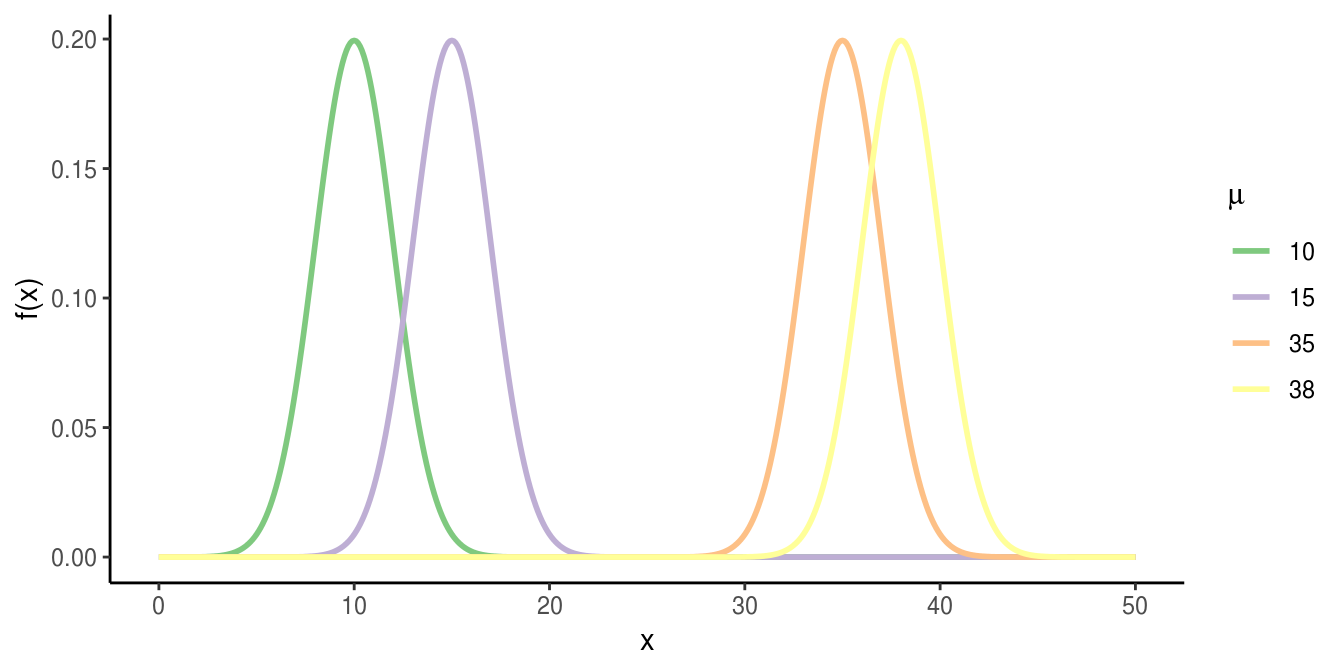
\includegraphics{anova_files/figure-latex/distr-normales-1.pdf}
\caption{\label{fig:distr-normales}Densidad de distribuciones de cuatro
distribuciones normales con igual varianza y distinta media}
\end{figure}

La Figura \ref{fig:distr-normales} ilustra estas condiciones: la
normalidad de la distribución en probabilidades y la variabilidad
constante. Las distribuciones en probabilidad difieren sólo con respecto
a sus medias. El análisis de los datos de las muestras de las
distribuciones en probabilidades de los niveles de los factores se
desarrolla usualmente en dos pasos:

Determinar si las medias de los niveles de los factores son las mismas.

Si las medias de los niveles del factor no son las mismas, examinar como
difieren y cuales son las consecuencias de las diferencias.

\hypertarget{comprobacion-de-los-supuestos}{%
\section{Comprobación de los
Supuestos}\label{comprobacion-de-los-supuestos}}

Los modelos de ANOVA son razonablemente robustos, aunque se produzcan
ciertos alejamientos del supuesto de normalidad.

\hypertarget{prueba-para-igualdad-de-varianzas}{%
\subsection{Prueba para igualdad de
varianzas}\label{prueba-para-igualdad-de-varianzas}}

\hypertarget{prueba-de-bartlett}{%
\subsubsection{Prueba de Bartlett}\label{prueba-de-bartlett}}

Las hipótesis son

\[
\begin{aligned}
 H_{0} &: \sigma_{1}^{2} = \sigma_{2}^{2} = \ldots = \sigma_{i}^{2} = \ldots = \sigma_{I}^{2} \\
 H_{a} &: \text{no todos}\ \text{los}\ \sigma_{i}^{2}\ \text{son}\ \text{iguales}
\end{aligned}
\]

Sean \(S_{1}^{2},\ldots,S_{I}^{2}\)indican las varianzas muestrales de
\(I\) poblaciones normales, y \(Gl_{i}\) indica los grados de libertad
asociados con la varianza muestral \(S_{i}^{2}\).

Bartlett ha demostrado que una función de
\(\left\lbrack \ln\left( C\text{MD} \right) - ln(MGD) \right\rbrack\),
(\(M\text{GD}\): media geométrica pesada; \(C\text{MD}\): cuadrado medio
dentro) para grandes tamaños muestrales, sigue aproximadamente la
distribución \(\chi^{2}\) con \((I-1)\) grados de libertad cuando las
varianzas poblacionales son iguales. La prueba estadística es:

\[
B = \frac{GL_{t}}{C}\left\lbrack \ln\left( CM_D \right) - ln(M\text{MGD}) \right\rbrack
\]

, donde

\[
C = 1 + \frac{1}{3\left( I - 1 \right)}\left\lbrack \left( \sum_{i = 1}^{I}\frac{1}{GL_{i}} \right) - \frac{1}{GL_{T}} \right\rbrack
\]

El término C es siempre mayor que 1.

La prueba estadística se reduce a:

\[
B = \frac{1}{C}\left\lbrack (GL_{t})\ln\left( CM_D \right) - \sum_{i = 1}^{I}\left( GL_{i} \right)lnS_{i}^{2} \right\rbrack
\]

se calcula el estadístico \(B\). La regla de decisión es:

Si \(B < \chi_{(1 - \alpha;I - 1)}^{2}\), no se rechaza \(H_{0}\)

Si \(B > \chi_{(1 - \alpha;I - 1)}^{2}\), se rechaza \(H_{0}\)

Esta aproximación se considera apropiada cuando los grados de libertad
son mayores o iguales que cuatro.

Cuando la prueba se usa para un modelo de ANOVA de un factor se tiene:

\(GL_{i} = n_{i} - 1\) y
\(GL_{T} = \sum_{i = 1}^{I}\left( n_{i} - 1 \right) = N - I\)

La prueba de Bartlett es bastante sensible a la falta de normalidad. Si
las varianzas muestrales son menores que la unidad, sus logaritmos serán
negativos. Por lo tanto, es conveniente utilizar un código
multiplicativo para hacer las varianzas mayores que la unidad. Este
código no afecta en modo alguno a la prueba estadística.

\hypertarget{prueba-de-levene-modificada}{%
\subsubsection{Prueba de Levene
Modificada}\label{prueba-de-levene-modificada}}

Las hipótesis son

\[
\begin{aligned}
H_{0} &:\sigma_{1}^{2} = \sigma_{2}^{2} = \ldots = \sigma_{i}^{2} = \ldots = \sigma_{I}^{2}\\
H_{a} &:\text{no todos}\ \text{los}\ \sigma_{i}^{2}\ \text{son}\ \text{iguales}
\end{aligned}
\]

Primero se calcula la desviación absoluta de las \(Y_ij\) observaciones
de sus respectivas medianas del nivel del factor \(\tilde{Y_{i}}\)

\[
d_{ij} = \left| Y_{ij} - \tilde{Y_{i}} \right|
\]

Entonces la prueba de Levene determina si los valores esperados de las
desviaciones absolutas son iguales. Si las varianzas son iguales
entonces los valores esperados de las desviaciones absolutas también
serán iguales. La prueba de Levene usa el estadístico \(F^{*}\)

\[
F_{L}^{*} = \frac{CM_{ET}}{CM_D}
\]

donde

\[
CM_{ET} = \frac{\sum n_{i}\left( \overline{d}_{i\bullet}\  - \overline{d}_{\bullet\bullet} \right)^{2}}{I - 1}
\]

\[
CM_D = \frac{\sum\sum\left( \overline{d}_{ij}\  - \overline{d}_{i\bullet}\right)^{2}}{N - 1}
\]

\[
\overline{d}_{i\bullet} = \sum_{j}^{}\frac{d_{ij}}{n_{i}}
\]

\[
\overline{d}_{\cdot \cdot } = \frac{\sum_{}^{}{\sum_{}^{}{d_{ij}}}}{N}
\]

Si las varianzas son iguales y los tamaños muestrales no son
extremadamente pequeños, \(\mathbf{F}_{\mathbf{L}}^{\mathbf{*}}\) sigue
aproximadamente una distribución \(F\) con \((I - 1)\) y \((N - I)\)
grados de libertad.

\hypertarget{prueba-de-kolmogorov---smirnov-modificacion-de-lilliefors-para-estudiar-normalidad}{%
\subsection{Prueba de Kolmogorov - Smirnov (modificación de Lilliefors)
para estudiar
Normalidad}\label{prueba-de-kolmogorov---smirnov-modificacion-de-lilliefors-para-estudiar-normalidad}}

Dada una muestra aleatoria, se calcula su media y su varianza muestral,
luego se calculan los datos normalizados \(Z_{i}\). Se ordenan los datos
de menor a mayor, se calculan las frecuencias acumuladas observadas, las
esperadas para los \(Z_{i}\), y luego se calculan las diferencias, en
valor absoluto entre las frecuencias acumuladas observadas y las
esperadas. Se define \(D_{max} = max\left| F_{i} - \hat{F_{i}} \right|\)
este estadístico se compara con el valor de tablas \(d_{max}\) al nivel
de significación \(\alpha\).

\hypertarget{residuos}{%
\subsection{Residuos}\label{residuos}}

El residuo \(\varepsilon_{ij}\) es definido como la diferencia entre el
valor observado y el ajustado:

\[
\varepsilon_{ij} = y_{ij} - \overline{y}_{i\bullet}
\]

Así, un residuo representa la desviación de una observación individual
de la respectiva media estimada del nivel del factor. A veces es útil
trabajar con los residuos estandarizados, que se expresan como:

\[
\varepsilon_{\ _{ij}}^{\otimes} = \frac{\varepsilon_{ij} - \overline{\varepsilon}}{\sqrt{CM_D}}
\]

Los residuos ``\emph{semistudentizados}'', los residuos
``\emph{studentizados}'', y los residuos ``\emph{studentizados
borrados}'' son a menudo útiles para diagnosticar los alejamientos del
modelo de ANOVA.

Los residuos ``\emph{semistudentizados}'' se calculan como:

\[
\varepsilon_{\ _{ij}}^{*} = \frac{\varepsilon_{ij}}{\sqrt{CM_D}}
\]

Los residuos ``\emph{studentizados}'' se calculan como:

\[
r_{ij} = \frac{\varepsilon_{ij}}{S\left( \varepsilon_{ij} \right)}
\]

donde

\[
S\left( \varepsilon_{ij} \right) = \sqrt{\frac{CM_D\left( n_{i} - 1 \right)}{n_{i}}}
\]

Finalmente, los residuos ``\emph{studentizados borrados}'' se calculan

\[
t_{ij} = \varepsilon_{ij}\left\lbrack \frac{N - I - 1}{SC_D\left( 1 - \frac{1}{n_{i}} \right)\varepsilon_{ij}^{2}} \right\rbrack^{\frac{1}{2}}
\]

\hypertarget{graficos-de-residuos}{%
\subsection{Gráficos de Residuos}\label{graficos-de-residuos}}

Estos gráficos son muy importantes para el diagnóstico de problemas con
el modelo. Incluye:

\begin{enumerate}
\def\labelenumi{\arabic{enumi}.}
\tightlist
\item
  \emph{Residuos vs.~las medias de tratamientos}: Dado que las valores
  ajustados de cada nivel de factor se corresponde a la media, todos los
  valores de los residuales de ese nivel se alinearán en sobre esa media
  (Figura \ref{fig:graficos-residuales}-a). Si no hay problemas con el
  modelo, entonces los residuales deberían tener la misma dispersión.
\end{enumerate}

2.Residuos vs.~el tiempo u otra secuencia: Si los datos fueron tomados
de forma aleatoria no debería verse un patrón definido (Figura
\ref{fig:graficos-residuales}-b).

\begin{enumerate}
\def\labelenumi{\arabic{enumi}.}
\setcounter{enumi}{2}
\item
  Gráficos de puntos de los residuos: Este gráfico es similar al
  primero. Denuevo, en todos lo niveles del factor los residuales
  deberían tener la misma dispersión alrededor del cero(Figura
  \ref{fig:graficos-residuales}-c). Además, dado que están graficados
  los residuales estandarizados, cualquier residual mayor 3 debería ser
  investigado por ser muy extremo.
\item
  Gráficos de probabilidad normal de los residuos: También llamado
  gráfico cuantil-cuantil o \emph{qqplot} (Figura
  \ref{fig:graficos-residuales}-d). Aquí se grafican los cuantiles de
  una normal teórica vs los cuantiles muestrales. Idealmente, deberían
  seguir una línea recta de pendiente 1 y ordenada 0.
\end{enumerate}






\begin{figure}
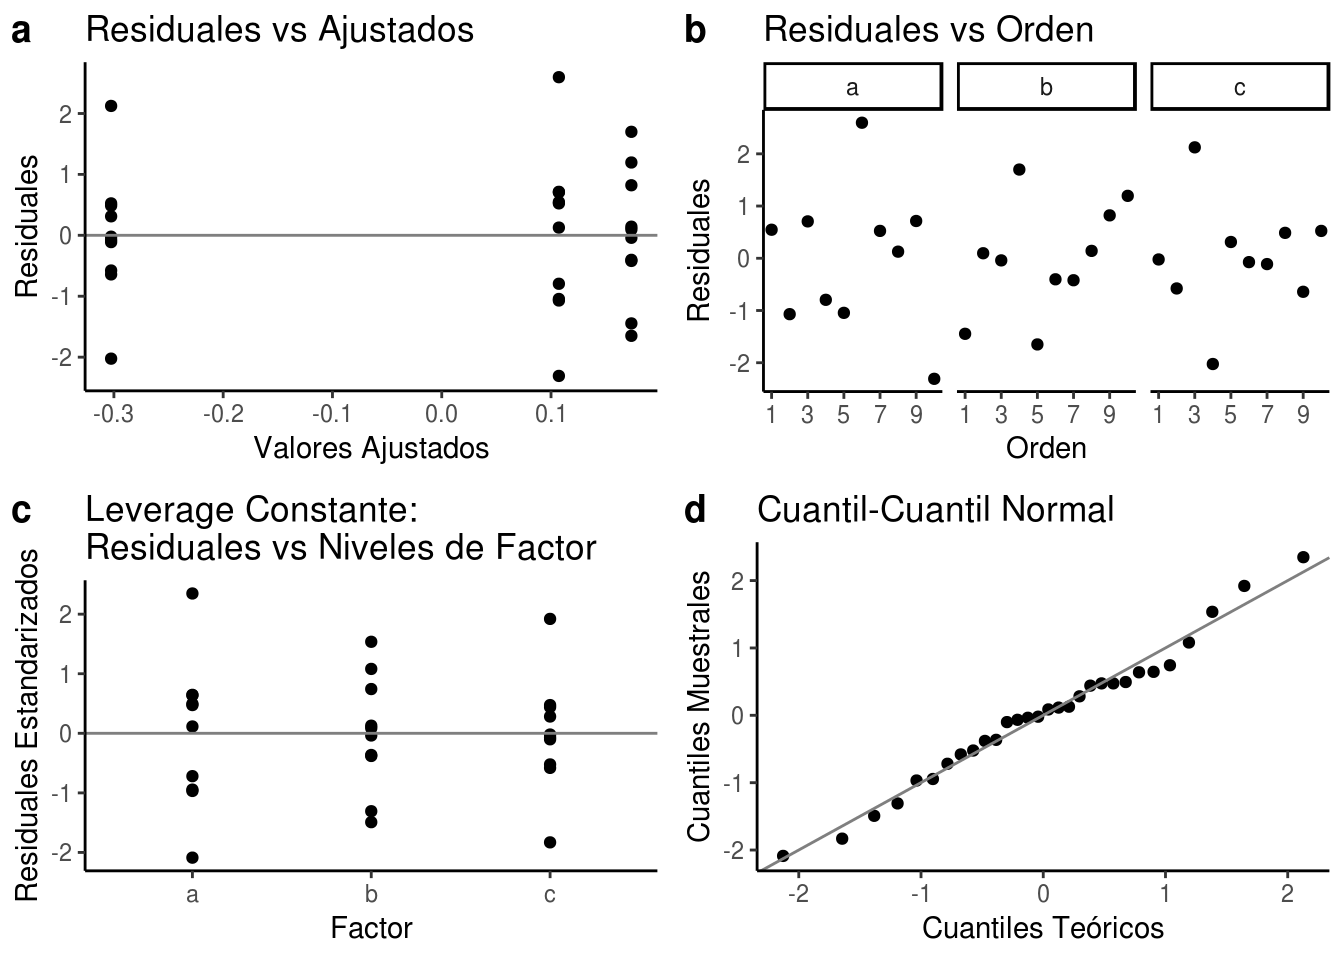
\includegraphics[width=1\linewidth]{anova_files/figure-latex/graficos-residuales-1} \caption{Gráficos de residuales para modelos de ANOVA.
a - residuales vs valores predichos. b - residuales vs orden de toma de
datos. c - residuales vs niveles del factor. d - gráfico de probabilidad
normal.}\label{fig:graficos-residuales}
\end{figure}

\hypertarget{diagnostico-de-los-alejamientos-de-los-supuestos-del-modelo-de-anova}{%
\subsubsection{Diagnóstico de los alejamientos de los supuestos del
Modelo de
ANOVA}\label{diagnostico-de-los-alejamientos-de-los-supuestos-del-modelo-de-anova}}

\textbf{Heterogeneidad de Varianzas}: El Modelo de ANOVA requiere que
los términos del error tengan varianzas constantes para todos los
niveles del factor. Cuando los tamaños de las muestras son iguales o no
difieren mucho, esta suposición puede ser estudiada usando los residuos,
los residuos ``studentizados'' o los residuos ``semistudentizados''.
Gráficos de los residuos vs.~las medias de los niveles del factor o los
gráficos de puntos de los residuos son útiles. Cuando los tamaños de las
muestras difieren mucho, los residuos ``studentizados'' deberían ser
usados en estos gráficos. La constancia de la varianza del error se ve
en estos gráficos pues los puntos tienen aproximadamente la misma
dispersión alrededor del cero para cada nivel.

La Figura \ref{fig:hetero} muestra un caso en el que las varianzas de
los errores no son constantes. En este caso los términos del error del
nivel \emph{c} del factor tienen una varianza mayor que los otros dos
niveles del factor.





\begin{figure}
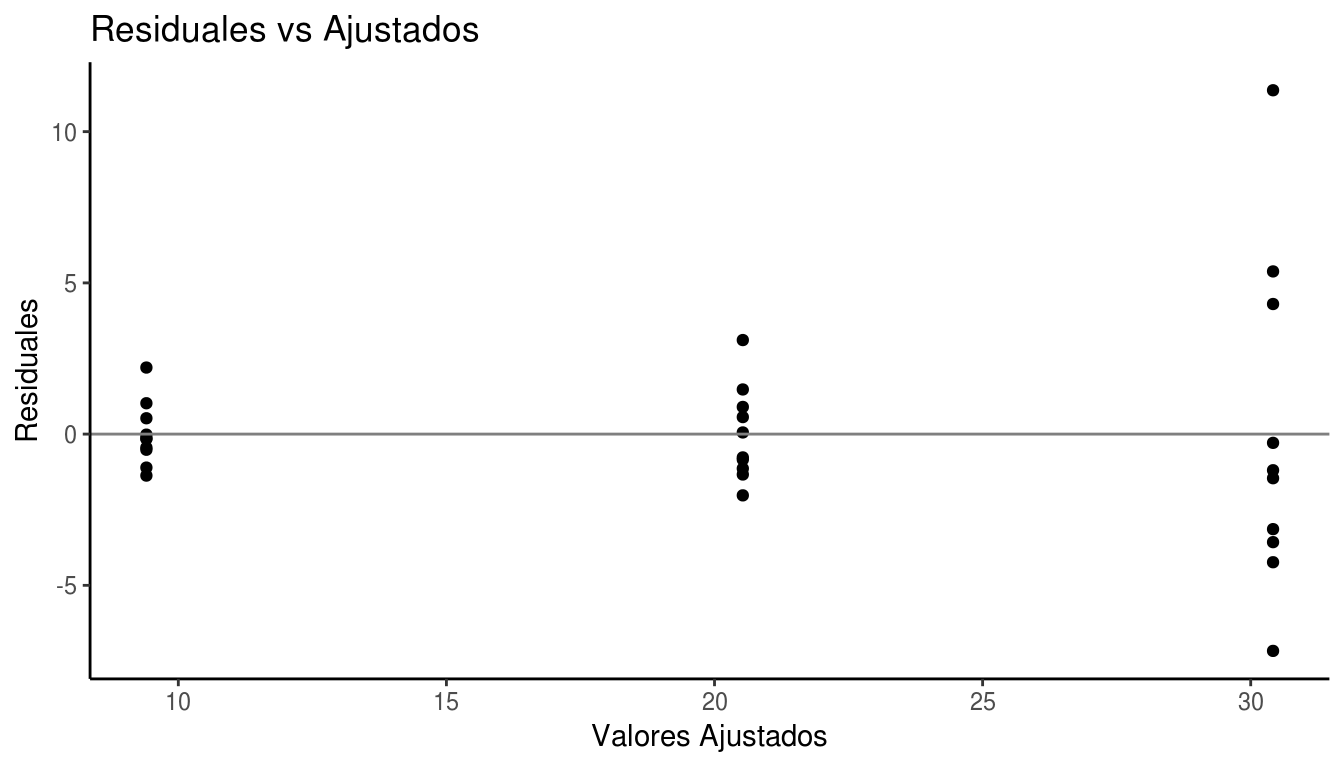
\includegraphics[width=0.5\linewidth]{anova_files/figure-latex/hetero-1} 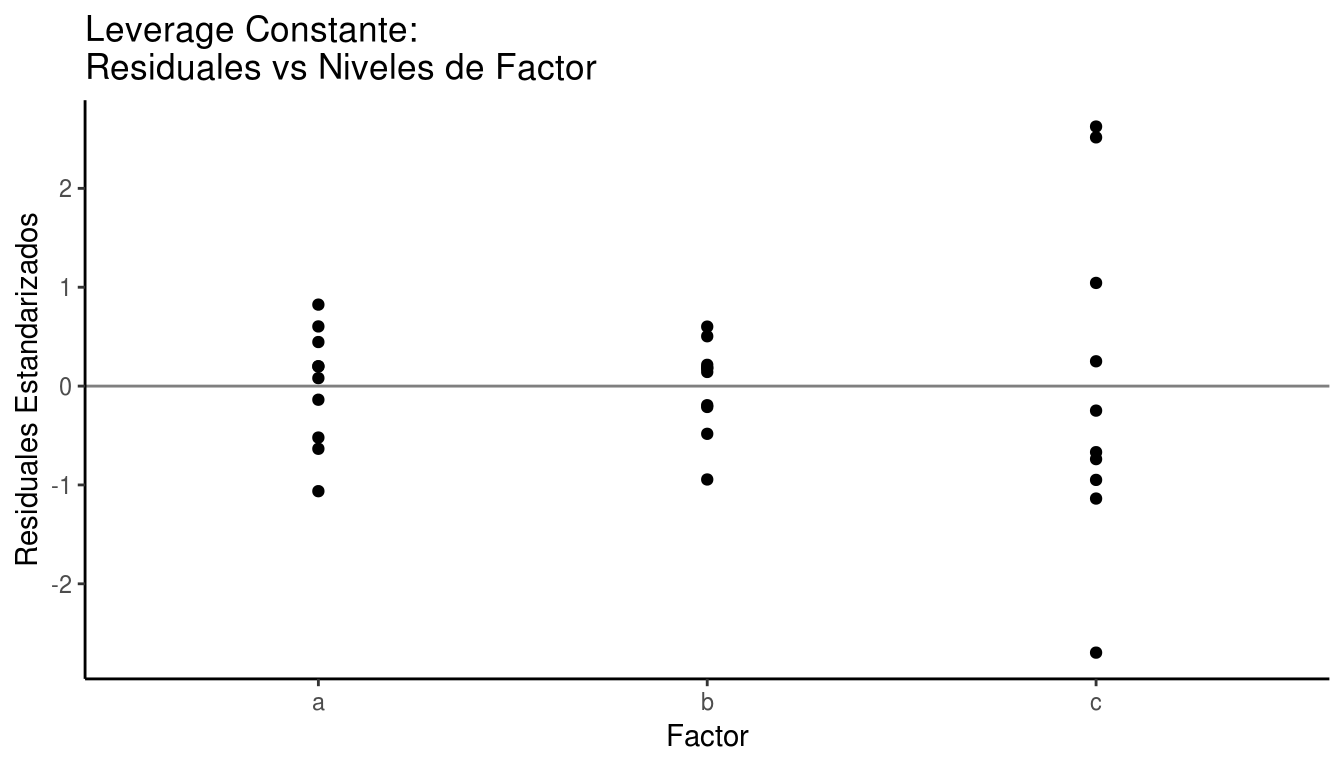
\includegraphics[width=0.5\linewidth]{anova_files/figure-latex/hetero-2} \caption{Residuales vs Valores Ajustados o predichos. Este gráfico
muestra que los residuales uno de los niveles muestra mayor dispersión
que el resto de los datos.}\label{fig:hetero}
\end{figure}

Cuando los tamaños de las muestras, para los diferentes niveles del
factor son grandes, los histogramas de los residuos para cada
tratamiento, son una manera efectiva de examinar la constancia de la
varianza de los términos del error.

\textbf{Falta de independencia en los términos del error:} En todos
aquellos casos en que los datos son obtenidos en una secuencia de
tiempo, un gráfico de secuencia de residuos es aconsejable para examinar
si los términos del error están correlacionados. La Figura
\ref{fig:indpen} muestra un caso en el cual los residuos aparecen
altamente correlacionados. Esto puede pasar porque el operario tiende a
sobreestimar a medida que pasa el tiempo o también porque los equipos se
descalibran.




\begin{figure}
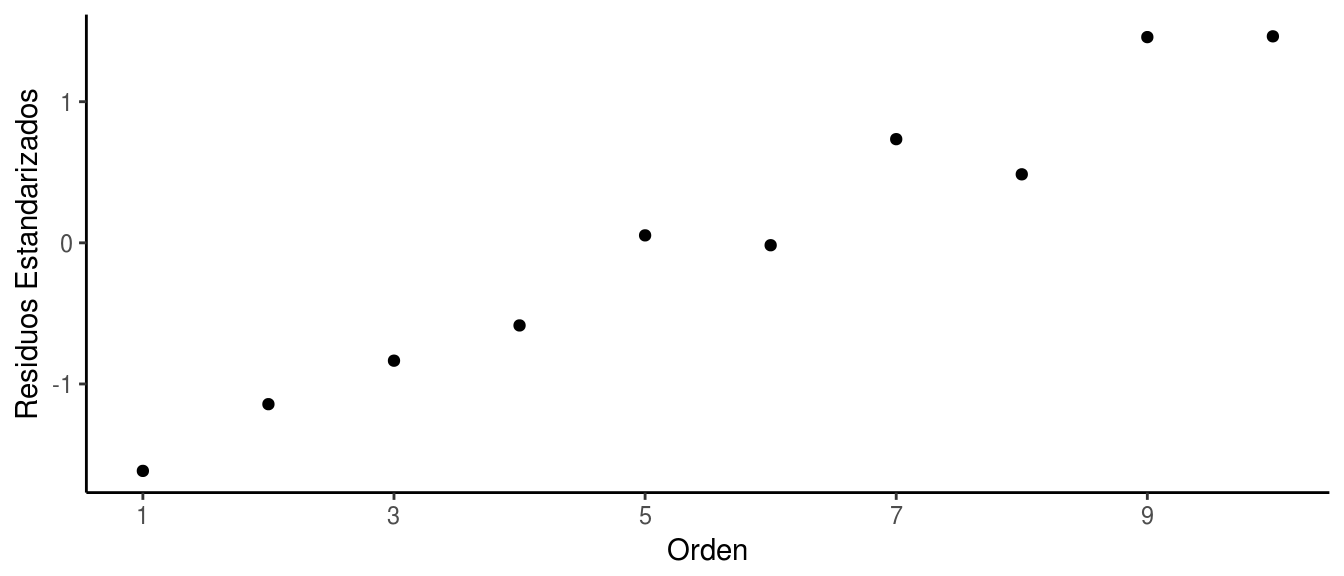
\includegraphics[width=0.75\linewidth]{anova_files/figure-latex/indpen-1} \caption{Residuales vs Orden. Los residuales muestran falta de
independencia al haber una correlación entre ellos.}\label{fig:indpen}
\end{figure}

La siguiente Figura \ref{fig:varianza-decrece} muestra un caso donde la
varianza decrece con el tiempo.





\begin{figure}
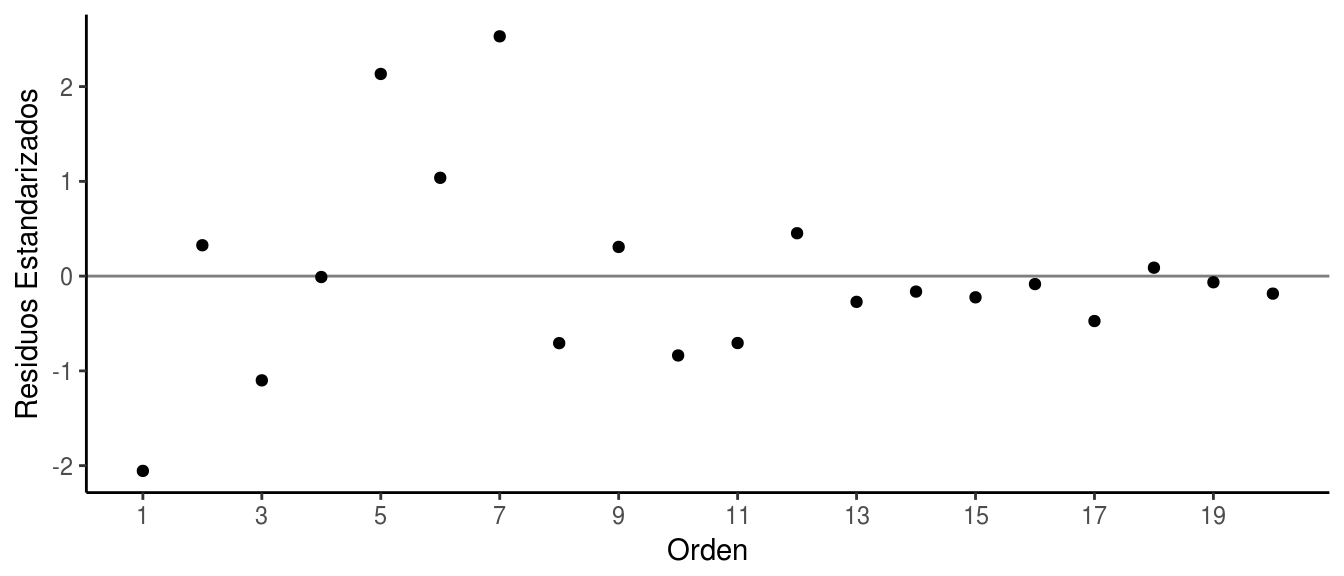
\includegraphics[width=0.75\linewidth]{anova_files/figure-latex/varianza-decrece-1} \caption{Residuales vs Orden. Los residuales muestran que
la varianza decrece, ya que al principio son mayores y al final son
menores}\label{fig:varianza-decrece}
\end{figure}

Cuando los datos son ordenados en alguna a otra secuencia lógica, tal
como una secuencia geográfica, también debe verificarse si existe
correlación entre los términos del error de acuerdo a este orden.

\textbf{Otros usos del análisis de residuos}: Este tipo de análisis se
puede usar para detectar ``outliers''. También es útil para determinar
si modelo de ANOVA de un factor es el adecuado; pues puede determinar la
omisión de alguna variable importante que explica las observaciones.
También puede ser usado para determinar la falta de normalidad de los
términos del error. Esto se realiza graficando los cuantiles de los
residuales observados vs los esperados.

\hypertarget{transformaciones}{%
\section{Transformaciones}\label{transformaciones}}

\hypertarget{transformaciones-para-estabilizar-las-varianzas}{%
\subsection{Transformaciones para estabilizar las
Varianzas}\label{transformaciones-para-estabilizar-las-varianzas}}

Varianza \emph{proporcional a} \(\mu_{i}\) : El estadístico muestral
\(\mathbf{S}_\mathbf{i}^\mathbf{2}\mathbf{/}{\overline{\mathbf{Y}}}_{\mathbf{i}}\)
tenderá a ser constante. Este tipo de situaciones a menudo se encuentra
cuando la variable observada es un número entero. Para estos casos, una
transformación raíz cuadrada es útil para estabilizar la varianza:

\(Y^{'} = \sqrt{Y}\)o \(Y^{'} = \sqrt{Y + \frac{1}{2}}\)
o\(Y^{'} = \sqrt{Y} + \sqrt{Y + 1}\)

\emph{Desviación estándar proporcional a} \(\mu_{i}\):
\(\mathbf{S}_\mathbf{i}\mathbf{/}\overline{\mathbf{Y}_\mathbf{i}}\)tiende
a ser contante para los diferentes niveles del factor. Una
transformación útil para estabilizar la varianza es la transformación
logarítmica:

\(Y^{'} = \log Y\)\emph{o}\(Y^{'} = \log{(Y + 1)}\)

\emph{Desviación estándar proporcional a} \(\mu_{i}^{2}\):
\(\mathbf{S}_\mathbf{i}^{\mathbf{2}}\mathbf{/}\overline{\mathbf{Y}}_{\mathbf{i}}^{\mathbf{2}}\)En
este caso tiende a ser constante. la transformación apropiada es la
recíproca:

\[
Y^{'} = \frac{1}{Y}
\]

\emph{La variable dependiente es una proporción}: Una transformación
apropiada para este caso es la transformación angular o arcoseno:

\[
Y^{'} = \text{arcsen}\sqrt{Y}
\]

\hypertarget{transformaciones-para-corregir-la-falta-de-normalidad}{%
\subsection{Transformaciones para corregir la falta de
normalidad}\label{transformaciones-para-corregir-la-falta-de-normalidad}}

La transformación que ayuda a corregir la heterogeneidad de varianzas
usualmente también es efectiva para hacer que las distribuciones de los
términos del error sean más normales.

\hypertarget{efectos-del-alejamiento-de-los-supuestos-del-modelo}{%
\subsection{Efectos Del Alejamiento De Los Supuestos Del
Modelo}\label{efectos-del-alejamiento-de-los-supuestos-del-modelo}}

\hypertarget{normalidad}{%
\subsubsection{Normalidad}\label{normalidad}}

Para el modelo I de ANOVA, la falta de normalidad no es importante, en
tanto ese alejamiento no sea extremo. La kurtosis es más importante que
la asimetría en términos de efectos sobre las inferencias (Figura
\ref{fig:kurtosis}).

La prueba F es poco afectada por la falta de normalidad, ya sea en
términos del nivel de significación o de la potencia de la prueba. Para
el Modelo II de ANOVA, la falta de normalidad tiene serias
implicaciones.

\begin{figure}
\centering
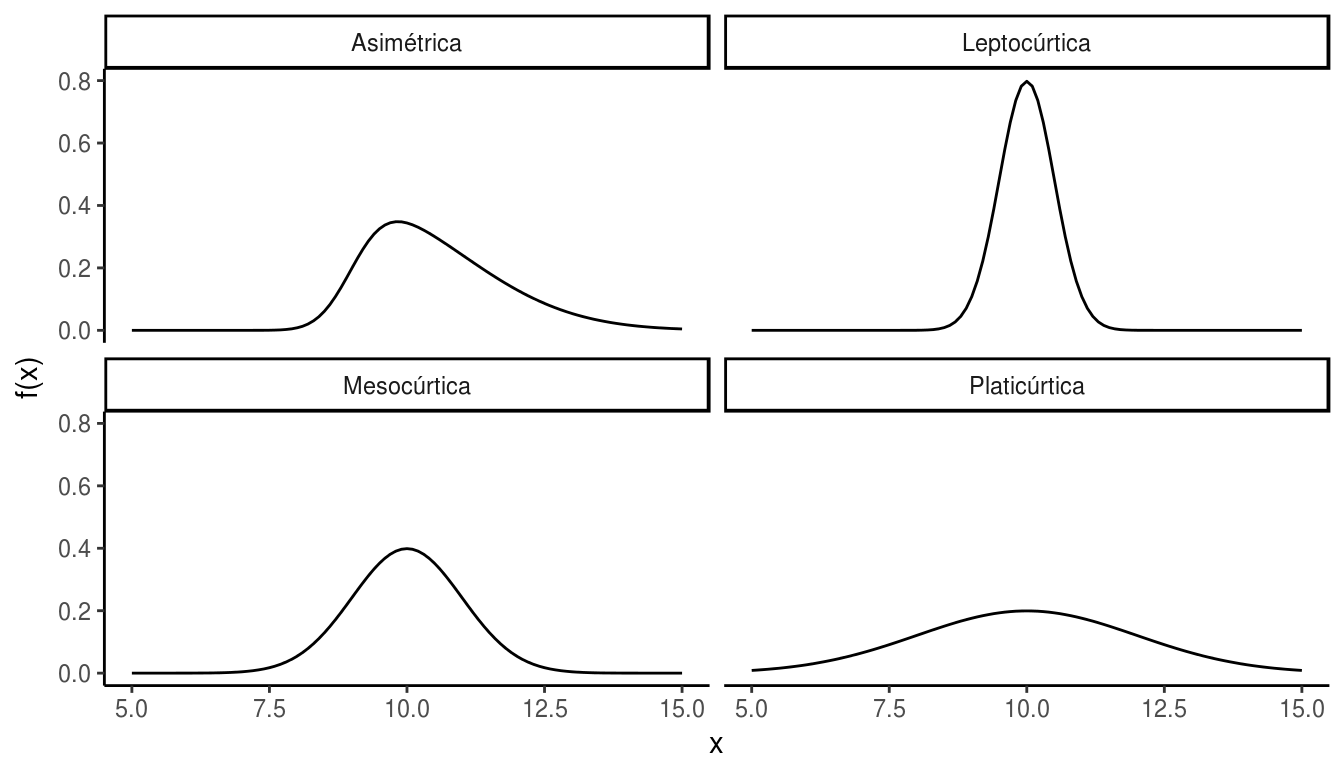
\includegraphics{anova_files/figure-latex/kurtosis-1.pdf}
\caption{\label{fig:kurtosis}Funciones de densidad para curvas asimétrica,
mesocúrtica, leptocúrtica, platicúrtica}
\end{figure}

\hypertarget{heterogeneidad-de-varianzas}{%
\subsubsection{Heterogeneidad de
varianzas}\label{heterogeneidad-de-varianzas}}

Para el modelo de efectos fijos, la prueba de F es ligeramente afectada
si los tamaños muestrales son iguales o no difieren mucho. La prueba de
F y los análisis relacionados son robustos frente a la heterogeneidad de
varianzas cuando los tamaños muestrales son aproximadamente iguales.

Para el modelo de efectos aleatorios, la heterogeneidad de varianzas
puede tener efectos pronunciados sobre las inferencias acerca de los
componentes de la varianza, aun con tamaños muestrales iguales.

\hypertarget{independencia-de-los-terminos-del-error}{%
\subsubsection{Independencia de los términos del
error}\label{independencia-de-los-terminos-del-error}}

La falta de independencia puede tener serios efectos sobre las
inferencias en el análisis de la varianza, para el modelo de efectos
fijos y para el de efectos aleatorios.

\hypertarget{formulacion-del-modelo-i-de-anova.}{%
\section{Formulación Del Modelo I De
ANOVA.}\label{formulacion-del-modelo-i-de-anova.}}

Denotaremos por I el número de niveles del factor bajo estudio, y
denotaremos cualquiera de estos niveles por el subíndice
\(i\ (i\  = \ 1,\ 2,\ \ldots,\
I)\). El número de casos para el i-ésimo nivel del factor es simbolizado
por \(n_{i}\), y el número total de casos en el estudio es denotado por
\(N\), donde:

\[
N = \sum_{i = 1}^{I}n_{i}
\]

Además, \(Y_{ij}\) denotará la j-ésima observación para el i-ésimo nivel
del factor. Dado que el número de casos para el i-ésimo nivel del factor
es denotado por \(n_{i}\), tendremos \(j\  = \ 1,\ 2,\ \ldots,\ n_{i}\).

El modelo I de ANOVA se puede plantear como sigue:

\[
y_{ij} = u_{i} + \varepsilon_{ij}
\]

donde:

\begin{itemize}
\item
  \(y_{ij}\) es el valor de la j-ésima observación para el i-ésimo nivel
  del factor o tratamiento.
\item
  \(\mu_{i}\) es un parámetro
\item
  \(\varepsilon_{ij}\) son variables independientes \(N(0,\sigma^{2})\)
\item
  \(i = 1,\ 2,\ldots,I;j = 1,\ 2,\ \ldots,\ n_{i}\)
\end{itemize}

\hypertarget{caracteristicas-importantes-del-modelo}{%
\subsection{Características importantes del
modelo}\label{caracteristicas-importantes-del-modelo}}

El valor observado de \(Y\) en el j-ésimo ensayo del i-ésimo nivel del
factor o tratamiento es la suma de dos componentes: a) un término
constante \(\mu_{i}\), y b) un término del error aleatorio
\(\varepsilon_{ij}\).

Dado que \(E\left( \varepsilon_{ij} \right) = 0\), se sigue que:

\[
E\left( Y_{ij} \right) = \mu_{i}
\]

Dado que \(\mu_{i}\) es una constante, se sigue que:

\[
V\text{ar}\left( Y_{ij} \right) = V\text{ar}\left( \varepsilon_{ij} \right) = \sigma^{2}
\]

Así como cada \(\varepsilon_{ij}\) esta normalmente distribuido, también
lo está cada \(Y_{ij}\).

Se asume que los términos del error son independientes

El modelo de ANOVA puede ser re-enunciado como:

\[
Y_{ij}\sim N(\mu_{i},\sigma^{2})
\]

\hypertarget{interpretacion-de-las-medias-de-los-niveles-del-factor}{%
\subsection{Interpretación De Las Medias De Los Niveles Del
Factor}\label{interpretacion-de-las-medias-de-los-niveles-del-factor}}

\textbf{Datos observacionales}: la media del nivel del factor
\(\mu_{i}\) corresponde a las medias para las diferentes poblaciones del
nivel del factor.

\textbf{Datos Experimentales}: la media del nivel del factor \(\mu_{i}\)
representa la media de la respuesta que debería obtenerse si el i-ésimo
tratamiento fuera aplicado a todas las unidades en la población de las
unidades experimentales sobre las cuales se harán las inferencias.

\hypertarget{ajustando-el-modelo}{%
\subsection{Ajustando El Modelo}\label{ajustando-el-modelo}}

Supongamos que tenemos \(I\) tratamientos o niveles de un factor y que
aplicamos cada uno de ellos a un grupo de unidades experimentales.Los
datos se podrían consignar de la siguiente forma:

\begin{longtable}[]{@{}llllllll@{}}
\toprule
\begin{minipage}[b]{0.11\columnwidth}\raggedright
~Tratamientos\strut
\end{minipage} & \begin{minipage}[b]{0.09\columnwidth}\raggedright
\(T_{1}\)\strut
\end{minipage} & \begin{minipage}[b]{0.09\columnwidth}\raggedright
\(T_{2}\)\strut
\end{minipage} & \begin{minipage}[b]{0.02\columnwidth}\raggedright
\(\ldots\)\strut
\end{minipage} & \begin{minipage}[b]{0.11\columnwidth}\raggedright
\(T_{i}\)\strut
\end{minipage} & \begin{minipage}[b]{0.02\columnwidth}\raggedright
\(\ldots\)\strut
\end{minipage} & \begin{minipage}[b]{0.11\columnwidth}\raggedright
\(T_{I}\)\strut
\end{minipage} & \begin{minipage}[b]{0.22\columnwidth}\raggedright
\strut
\end{minipage}\tabularnewline
\midrule
\endhead
\begin{minipage}[t]{0.11\columnwidth}\raggedright
\strut
\end{minipage} & \begin{minipage}[t]{0.09\columnwidth}\raggedright
\(y_{1\mathbf{1}}\)\strut
\end{minipage} & \begin{minipage}[t]{0.09\columnwidth}\raggedright
\(y_{2\mathbf{1}}\)\strut
\end{minipage} & \begin{minipage}[t]{0.02\columnwidth}\raggedright
\(\ldots\)\strut
\end{minipage} & \begin{minipage}[t]{0.11\columnwidth}\raggedright
\(y_{i1}\)\strut
\end{minipage} & \begin{minipage}[t]{0.02\columnwidth}\raggedright
\(\ldots\)\strut
\end{minipage} & \begin{minipage}[t]{0.11\columnwidth}\raggedright
\(y_{I1}\)\strut
\end{minipage} & \begin{minipage}[t]{0.22\columnwidth}\raggedright
\strut
\end{minipage}\tabularnewline
\begin{minipage}[t]{0.11\columnwidth}\raggedright
\strut
\end{minipage} & \begin{minipage}[t]{0.09\columnwidth}\raggedright
\(y_{1\mathbf{2}}\)\strut
\end{minipage} & \begin{minipage}[t]{0.09\columnwidth}\raggedright
\(y_{2\mathbf{2}}\)\strut
\end{minipage} & \begin{minipage}[t]{0.02\columnwidth}\raggedright
\(\ldots\)\strut
\end{minipage} & \begin{minipage}[t]{0.11\columnwidth}\raggedright
\(y_{i2}\)\strut
\end{minipage} & \begin{minipage}[t]{0.02\columnwidth}\raggedright
\(\ldots\)\strut
\end{minipage} & \begin{minipage}[t]{0.11\columnwidth}\raggedright
\(y_{I2}\)\strut
\end{minipage} & \begin{minipage}[t]{0.22\columnwidth}\raggedright
\strut
\end{minipage}\tabularnewline
\begin{minipage}[t]{0.11\columnwidth}\raggedright
\strut
\end{minipage} & \begin{minipage}[t]{0.09\columnwidth}\raggedright
\(\vdots\)\strut
\end{minipage} & \begin{minipage}[t]{0.09\columnwidth}\raggedright
\(\vdots\)\strut
\end{minipage} & \begin{minipage}[t]{0.02\columnwidth}\raggedright
\(\ddots\)\strut
\end{minipage} & \begin{minipage}[t]{0.11\columnwidth}\raggedright
\(\vdots\)\strut
\end{minipage} & \begin{minipage}[t]{0.02\columnwidth}\raggedright
\(\ldots\)\strut
\end{minipage} & \begin{minipage}[t]{0.11\columnwidth}\raggedright
\(\vdots\)\strut
\end{minipage} & \begin{minipage}[t]{0.22\columnwidth}\raggedright
\strut
\end{minipage}\tabularnewline
\begin{minipage}[t]{0.11\columnwidth}\raggedright
\strut
\end{minipage} & \begin{minipage}[t]{0.09\columnwidth}\raggedright
\(y_{1j}\)\strut
\end{minipage} & \begin{minipage}[t]{0.09\columnwidth}\raggedright
\(y_{2j}\)\strut
\end{minipage} & \begin{minipage}[t]{0.02\columnwidth}\raggedright
\(\ldots\)\strut
\end{minipage} & \begin{minipage}[t]{0.11\columnwidth}\raggedright
\(y_{i\mathbf{j}}\)\strut
\end{minipage} & \begin{minipage}[t]{0.02\columnwidth}\raggedright
\(\ldots\)\strut
\end{minipage} & \begin{minipage}[t]{0.11\columnwidth}\raggedright
\(y_{I\mathbf{j}}\)\strut
\end{minipage} & \begin{minipage}[t]{0.22\columnwidth}\raggedright
\strut
\end{minipage}\tabularnewline
\begin{minipage}[t]{0.11\columnwidth}\raggedright
\(\sum_{j = \mathbf{1}}^{n_{i}}y_{i\mathbf{j}}\)\strut
\end{minipage} & \begin{minipage}[t]{0.09\columnwidth}\raggedright
\(\sum_{j = \mathbf{1}}^{n_{1}}y_{1j}\)\strut
\end{minipage} & \begin{minipage}[t]{0.09\columnwidth}\raggedright
\(\sum_{j = \mathbf{1}}^{n_{2}}y_{2j}\)\strut
\end{minipage} & \begin{minipage}[t]{0.02\columnwidth}\raggedright
\(\ldots\)\strut
\end{minipage} & \begin{minipage}[t]{0.11\columnwidth}\raggedright
\(\sum_{j = \mathbf{1}}^{n_{i}}y_{i\mathbf{j}}\)\strut
\end{minipage} & \begin{minipage}[t]{0.02\columnwidth}\raggedright
\(\ldots\)\strut
\end{minipage} & \begin{minipage}[t]{0.11\columnwidth}\raggedright
\(\sum_{j = \mathbf{1}}^{n_{I}}y_{I\mathbf{j}}\)\strut
\end{minipage} & \begin{minipage}[t]{0.22\columnwidth}\raggedright
\(\sum_{j = \mathbf{1}}^{I}y_{i\mathbf{j}}\)\strut
\end{minipage}\tabularnewline
\begin{minipage}[t]{0.11\columnwidth}\raggedright
\strut
\end{minipage} & \begin{minipage}[t]{0.09\columnwidth}\raggedright
\(n_{1}\)\strut
\end{minipage} & \begin{minipage}[t]{0.09\columnwidth}\raggedright
\(n_{2}\)\strut
\end{minipage} & \begin{minipage}[t]{0.02\columnwidth}\raggedright
\(\ldots\)\strut
\end{minipage} & \begin{minipage}[t]{0.11\columnwidth}\raggedright
\(n_{i}\)\strut
\end{minipage} & \begin{minipage}[t]{0.02\columnwidth}\raggedright
\(\ldots\)\strut
\end{minipage} & \begin{minipage}[t]{0.11\columnwidth}\raggedright
\(n_{I}\)\strut
\end{minipage} & \begin{minipage}[t]{0.22\columnwidth}\raggedright
\(\sum_{i = \mathbf{1}}^{I}n_{i} = N\)\strut
\end{minipage}\tabularnewline
\begin{minipage}[t]{0.11\columnwidth}\raggedright
\(\overline{y_{i\bullet}}\)\strut
\end{minipage} & \begin{minipage}[t]{0.09\columnwidth}\raggedright
\(\overline{y_{1.}}\)\strut
\end{minipage} & \begin{minipage}[t]{0.09\columnwidth}\raggedright
\(\overline{y_{2.}}\)\strut
\end{minipage} & \begin{minipage}[t]{0.02\columnwidth}\raggedright
\(\ldots\)\strut
\end{minipage} & \begin{minipage}[t]{0.11\columnwidth}\raggedright
\(\overline{y_{i\bullet}}\)\strut
\end{minipage} & \begin{minipage}[t]{0.02\columnwidth}\raggedright
\(\ldots\)\strut
\end{minipage} & \begin{minipage}[t]{0.11\columnwidth}\raggedright
\(\overline{y_{I.}}\)\strut
\end{minipage} & \begin{minipage}[t]{0.22\columnwidth}\raggedright
\(\frac{\sum_{i\mathbf{j}}^{N}y_{i\mathbf{j}}}{N} = \overline{y_{\bullet\bullet}}\)\strut
\end{minipage}\tabularnewline
\begin{minipage}[t]{0.11\columnwidth}\raggedright
\strut
\end{minipage} & \begin{minipage}[t]{0.09\columnwidth}\raggedright
\(S_{1}^{2}\)\strut
\end{minipage} & \begin{minipage}[t]{0.09\columnwidth}\raggedright
\(S_{2}^{2}\)\strut
\end{minipage} & \begin{minipage}[t]{0.02\columnwidth}\raggedright
\(\ldots\)\strut
\end{minipage} & \begin{minipage}[t]{0.11\columnwidth}\raggedright
\(S_{i}^{2}\)\strut
\end{minipage} & \begin{minipage}[t]{0.02\columnwidth}\raggedright
\(\ldots\)\strut
\end{minipage} & \begin{minipage}[t]{0.11\columnwidth}\raggedright
\(S_{I}^{2}\)\strut
\end{minipage} & \begin{minipage}[t]{0.22\columnwidth}\raggedright
\strut
\end{minipage}\tabularnewline
\bottomrule
\end{longtable}

donde

\(T_{i}\) es el tratamiento o nivel del factor \(i\); con
\(i\  = \ 1,\ 2,\ldots,I\)

\(y_{ij}\) es la observación sobre la unidad experimental\(\ j\) con el
tratamiento \(i\); \$~j~ = ~1,2,~\ldots,~n\_\{i\}\$.

\(N\) tamaño de la muestra

\({\overline{y}}_{i \bullet}\) es la media muestral de cada tratamiento.

\(n_{i}\) es el número de observaciones con el tratamiento \(i\)

\({\overline{y}}_{\bullet \bullet}\) es la media total, para todas las
observaciones.

\(S_{i}^{2}\) es la varianza muestral para el tratamiento \(i\)

\hypertarget{estimadores-de-minimos-cuadrados}{%
\subsection{Estimadores De Mínimos
Cuadrados}\label{estimadores-de-minimos-cuadrados}}

De acuerdo al criterio de mínimos cuadrados la suma de los cuadrados de
las desviaciones de las observaciones alrededor de sus valores esperados
puede ser minimizada con respecto a los parámetros. Para un modelo de
ANOVA, tenemos que:

\[
E\left( Y_{ij} \right) = \mu_{i}
\]

Así, la cantidad a ser minimizada es:

\[
\sum_{i}^{}{\sum_{j}^{}\left( y_{ij} - \mu_{i} \right)^{2}}
\]

Esta expresión se puede escribir como:

\[
\sum_{j}^{}\left( y_{1j} - \mu_{1} \right)^{2} + \sum_{j}^{}\left( y_{2j} - \mu_{2} \right)^{2} + \ldots + \sum_{j}^{}\left( y_{Ij} - \mu_{I} \right)^{2}
\]

La media muestral minimiza una suma de desviaciones al cuadrado

\begin{equation}
  \hat{\mu_{i}} = \overline{y}_{i\bullet}
  \label{eq:minimoscuadrados}
\end{equation}

\hypertarget{comentarios}{%
\subsubsection{Comentarios}\label{comentarios}}

\begin{enumerate}
\def\labelenumi{\arabic{enumi}.}
\item
  Los estimadores de mínimos cuadrados \eqref{eq:minimoscuadrados} son
  también estimadores de máxima verosimilitud para el error normal
  (\(\varepsilon_{ij}\)) del modelo de ANOVA.
\item
  Para derivar el estimador de mínimo cuadrados de \(u_{i}\) , es
  necesario minimizar, con respecto a \(u_{i}\), el i-ésimo componente
  de la suma de cuadrados en:
\end{enumerate}

\[
\sum_{j}^{}\left( y_{ij} - \mu_{i} \right)^{2}
\]

Diferenciando con respecto a \(\mu_{i}\), se obtiene:

\[
\frac{\partial\sum_{j}^{}\left( y_{ij} - \mu_{i} \right)^{2}}{\partial\mu_{i}} = \sum_{}^{}{- 2\left( y_{ij} - \mu_{i} \right)}
\]

Esta derivada se iguala a cero y se reemplaza el parámetro \(\mu_{i}\)
por su estimador:

\[
- 2\sum_{j = 1}^{n_{i}}\left( y_{ij} - \mu_{i} \right) = 0
\]

\[
\sum_{j = 1}^{n_{i}}y_{ij} = n_{i}\hat{\mu_{i}}
\]

\[
\hat{\mu_{i}} = \overline{Y}_{i\bullet}
\]

\hypertarget{particion-de-la-suma-de-cuadrados-total}{%
\section{Partición De La Suma De Cuadrados
Total}\label{particion-de-la-suma-de-cuadrados-total}}

La variabilidad total de las observaciones \(y_{ij}\), sin usar la
información sobre los niveles del factor, es medida en términos de la
desviación de cada observación \(y_{ij}\) alrededor de la media total
\({\overline{y}}_{\bullet\bullet}\):

\[
y_{ij} - {\overline{y}}_{\bullet\bullet}
\]

Cuando se utiliza la información sobre los niveles del factor, las
desviaciones son aquellas de cada observación \(y_{ij}\) alrededor de su
respectiva media estimada \({\overline{y}}_{\text{i}\bullet}\):

\[
y_{ij} - {\overline{y}}_{\text{i}\bullet}
\]

La diferencia entre la desviación total y la desviación anterior refleja
la diferencia entre la media estimada del nivel del factor y la media
total:

\[
{(y}_{ij} - {\overline{y}}_{\bullet\bullet}) - (y_{ij} - {\overline{y}}_{i}) = {\overline{y}}_{\text{i}\bullet} - {\overline{y}}_{\bullet\bullet}
\]

Así, la desviación total \(y_{ij} - {\overline{y}}_{\bullet\bullet}\)
puede ser vista como la suma de dos componentes:

La desviación de la media estimada del nivel del factor alrededor de la
media total.

La desviación de \(y_{ij}\) alrededor de la media de su nivel del
factor. Esta desviación es simplemente el residuo \(\varepsilon_{ij}\) .

Elevando al cuadrado se obtiene:

\[
\sum_{i}^{}{\sum_{j}^{}\left( y_{ij} - {\overline{y}}_{\bullet\bullet} \right)^{2}} = \sum_{i}^{}{n_{i}\left( {\overline{y}}_{\text{i}\bullet} - {\overline{y}}_{\bullet\bullet} \right)^{2}} + \sum_{i}^{}{\sum_{j}^{}\left( y_{ij} - {\overline{y}}_{\text{i}\bullet} \right)^{2}}
\]

El primer miembro de igualdad representa la variabilidad total de las
\(y_{ij}\) observaciones y es denotado como la \emph{suma de cuadrados
total (}\(SCT\)\emph{)}:

\[
SC_T = \sum_{i}^{}{\sum_{j}^{}\left( y_{ij} - {\overline{y}}_{\bullet\bullet} \right)^{2}}
\]

El primer término del segundo miembro de la igualdad será indicado como
\(SCE\), la \emph{suma de cuadrados entre} tratamientos:

\[
SC_E = \sum_{i}^{}{n_{i}\left( y_{\text{i}\bullet} - {\overline{y}}_{\bullet\bullet} \right)^{2}}
\]

El segundo término se indica como \(SCD\), la \emph{suma de cuadrados
dentro} de tratamientos o la \emph{suma de cuadrados del error}.

\[
SC_D = \sum_{i}^{}{\sum_{j}^{}\left( y_{ij} - {\overline{y}}_{\text{i}\bullet} \right)^{2}} = \sum_{i}^{}{\sum_{j}^{}\varepsilon_{ij}^{2}}
\]

Así, podemos escribir:

\[
SCT\  = \ SCE\  + \ SCD
\]

La suma total de los cuadrados para el modelo de análisis de la varianza
se compone en consecuencia de dos partes.

\hypertarget{formulas-computatorias}{%
\subsection{Fórmulas computatorias}\label{formulas-computatorias}}

\[
\begin{matrix}
SC_T = \sum_{i}^{}{\sum_{j}^{}{y_{ij}^{2} - N{\overline{y}}_{\bullet\bullet}^{2}}} \\
SC_E = \sum_{i}^{}{n_{i}y_{\text{i}\bullet}^{2} - N{\overline{y}}_{\bullet\bullet}^{2}} \\
SC_D = \sum_{i}^{}{\sum_{j}^{}{y_{ij}^{2} - n_{i}{\overline{y}}_{\text{i}\bullet}^{2}}} = SC_T - SC_E \\
\end{matrix}
\]

\hypertarget{grados-de-libertad}{%
\section{Grados De Libertad}\label{grados-de-libertad}}

Correspondiendo a la descomposición de la suma de cuadrados total, se
puede obtener los grados de libertad asociados.

La \(SCT\) tiene \((N -\ 1)\) grados de libertad asociados. Hay en
conjunto N desviaciones \(Y_{ij} - {\overline{Y}}_{\bullet\bullet}\) ,
pero un grado de libertad se pierde debido a que las desviaciones no son
independientes a causa de que la suma de ellas debe ser cero.

\(\sum_{i}^{}{\sum_{j}^{}\left(y_{ij} - {\overline{y}}_{\bullet\bullet} \right)} = 0\)

La \(SCE\) (entre tratamientos) tiene \((I -\ 1)\) grados de libertad
asociados. Hay I desviaciones de las medias de los niveles de los
factores
\({\overline{Y}}_{\text{i}\bullet} - {\overline{Y}}_{\bullet\bullet}\),
pero un grado de libertad se pierde porque las desviaciones no son
independientes a causa de que la suma pesada debe ser cero.
\(\sum_{i}^{}{n_{i}\left( y_{\text{i}\bullet} - {\overline{y}}_{\bullet\bullet} \right) = \ 0}\).

La \(SCD\) tiene \((N -\ I)\) grados de libertad asociados. Esto puede
verse considerando el componente de la \(SCD\) para el i-ésimo nivel del
factor:

\[
\sum_{j}^{}\left( y_{ij} - {\overline{y}}_{\text{i}\bullet} \right)^{2}
\]

La expresión es equivalente a la suma de cuadrados total considerando
sólo el i-ésimo nivel del factor. Así, hay \(n_{i}\  - \ 1\) grados de
libertad asociados con esta suma de cuadrados. De esta forma la \(SCD\)
es una suma de sumas de cuadrados, los grados de libertad asociados son
la suma de los grados de libertad de sus términos:

\[
(n_{1}\  - \ 1)\  + \ (n_{2}\  - \ 1)\  + \ \ldots\  + \ (n_{I}\  - \ 1)\  = \ N-\ I
\]

Los grados de libertad, al igual que la suma de cuadrados, son aditivos.

\hypertarget{cuadrados-medios}{%
\section{Cuadrados Medios}\label{cuadrados-medios}}

Los cuadrados medios se obtienen dividiendo la suma de cuadrados por sus
grados de libertad asociados. Se tiene:

\[
\begin{matrix}
CM_E = \frac{SC_E}{I - 1} \\
 \\
CM_D = \frac{SC_D}{N - I} \\
\end{matrix}
\]

\(CM_E\), es el cuadrado medio entre los tratamientos.

\(CM_D\), es el cuadrado medio dentro de los tratamientos o del error.

\hypertarget{esperanza-de-los-cuadrados-medios}{%
\subsection{Esperanza de los Cuadrados
Medios}\label{esperanza-de-los-cuadrados-medios}}

Los valores esperados del \(CM_D\) y \(CM_E\) pueden ser vistos como:

\[
E\left( CM_D \right) = \sigma^{2}
\]

\begin{equation}
E\left( CM_E \right) = \sigma^{2} + \frac{\sum_{}^{}{n_{i}\left( \mu_{i} - \mu_{\bullet} \right)^{2}}}{I - 1}
  (\#eq:eCM_E)
\end{equation}

donde

\[
\mu_{\bullet} = \frac{\sum_{}^{}{n_{i}\mu_{i}}}{N}
\]

\begin{enumerate}
\def\labelenumi{\arabic{enumi}.}
\item
  El \(CM_D\) es un estimador insesgado de la varianza del error llamado
  \(\varepsilon_{ij}\), tanto si las medias \(u_{i}\) son iguales como
  si no.
\item
  Cuando todas las medias \(\mu_i\) de los niveles del factor son
  iguales y por lo tanto iguales a la media pesada \(\mu_{\bullet}\),
  entonces\(\ E(CM_E) = \sigma^{2}\) dado que el segundo término se
  vuelve cero. Cuando las medias de los niveles del factor no son
  iguales, el \(CM_E\) tiende en promedio a ser mayor que el \(CM_D\),
  dado que el segundo término de la Ecuación @ref(eq:eCM\_E) será
  positivo. Esto es intuitivamente razonable, como se ilustra en la
  figura para cuatro tratamientos. En la situación planteada se asume
  que todos los tamaños muestrales son iguales, o sea\(\ n_{i} = n\).
  Cuando todos los \(\mu_{i}\) son iguales, entonces todos lo
  \(\overline{Y}_{i\bullet}\) siguen la misma distribución en el
  muestreo, con una media\(\mu_{c}\) y una varianza \(\sigma^{2}/n\).
  Cuando las \(\mu_{i}\) no son iguales, por otro lado,
  las\(\ {\overline{Y}}_{\text{i}\bullet}\) siguen diferentes
  distribuciones en el muestreo, cada una con la misma variabilidad
  \(\sigma^{2}/n\) pero centradas sobre medias diferentes \(\mu_{i}\)
  (Figura \ref{fig:distr-normales}).
\end{enumerate}

En consecuencia, los \({\overline{Y}}_{\text{i}\bullet}\) tenderán a
diferir unos de otros tanto si los \(\mu_i\) difieren como si son
iguales, y en consecuencia la \(SCE\) tenderá a ser mayor cuando las
medias de los niveles de los factores no son las mismas que cuando ellas
son iguales. Esta propiedad de la \(SCE\) es utilizada en la
construcción de la prueba estadística para determinar si las medias de
los niveles del factor son iguales o no. Si la \(SCE\) y la \(SCD\) son
de la misma magnitud, esto sugiere que las medias µi de los niveles del
factor son iguales. Si la \(SCE\) es substancialmente mayor que la
\(SCD\), esto sugeriría que los \(\mu_i\) no son iguales.

\hypertarget{comentarios-1}{%
\subsection{Comentarios}\label{comentarios-1}}

\begin{enumerate}
\def\labelenumi{\arabic{enumi}.}
\tightlist
\item
  Para encontrar el valor esperado del \(CM_D\), se ve que puede ser
  expresado como sigue:
\end{enumerate}

\[
\begin{matrix}
CM_D\  = \frac{1}{N - I}\sum_{i}^{}{\sum_{j}^{}\left( Y_{ij} - {\overline{Y}}_{\text{i}\bullet} \right)^{2}} \\
 = \frac{1}{N - I}\sum_{i}^{}\left\lbrack \left( n_{i} - 1 \right)\frac{\sum_{j}^{}\left( Y_{ij} - {\overline{Y}}_{\text{i}\bullet} \right)^{2}}{\left( n_{i} - 1 \right)} \right\rbrack \\
\end{matrix}
\]

Indicamos la varianza muestral de las observaciones para el i-ésimo
nivel del factor como \(s_{i}^{2}\):

\[
s_{i}^{2} = \frac{\sum_{j}^{}\left( Y_{ij} - {\overline{Y}}_{\text{i}\bullet} \right)^{2}}{n_{i} - 1}
\]

Por lo tanto, el \(CM_D\) puede ser expresado de la siguiente forma:

\[
CM_D = \frac{1}{N - I}\sum_{i}^{}{\left( n_{i} - 1 \right)s_{i}^{2}}
\]

Dado que la varianza muestral es un estimador insesgado de la varianza
poblacional, la cual es \(\sigma^{2}\) para todos los niveles del
factor, se obtiene:

\[
\begin{aligned}
E\left( CM_D \right)& = \frac{1}{N - I}\sum_{i}^{}{\left( n_{i} - 1 \right)E\left( s_{i}^{2} \right)} \\
& = \frac{1}{N - I}\sum_{i}^{}{\left( n_{i} - 1 \right)\sigma^{2}} \\
& = \sigma^{2} \\
\end{aligned}
\]

\begin{enumerate}
\def\labelenumi{\arabic{enumi}.}
\setcounter{enumi}{1}
\tightlist
\item
  Se puede derivar el valor esperado de la \(CM_E\) para el caso
  especial en que todos los tamaños muestrales ni son los mismos, o sea
  \(n_i = n\). El resultado general para este caso especial:
\end{enumerate}

\[
E\left( CM_E \right) = \sigma^{2} + \frac{n\sum_{}^{}\left( \mu_{i} - \mu_{\bullet} \right)^{2}}{I - 1}\text{ cuando}\ n_{i} = n
\]

De esta forma, cuando todos los tamaños muestrales de los niveles del
factor son \(n\), el \(CM_E\) se vuelve:

\[
CM_E = \frac{n\sum_{}^{}\left( {\overline{Y}}_{\text{i}\bullet} -
{\overline{Y}}_{\bullet\bullet} \right)^{2}}{I - 1}\text{ cuando }n_{i} = n
\]

Para derivar el \(E(CM_D)\), se considera el modelo:

\[
Y_{ij}\  = \ u_{i}\  + \ \varepsilon_{ij}
\]

Promediando el \(Y_{ij}\) para el i-ésimo nivel del factor, se obtiene:

\[
{\overline{Y}}_{i \bullet} = \mu_{i} + {\overline{\varepsilon}}_{i \bullet}
\]

donde \({\overline{\varepsilon}}_{i \bullet}\) es el promedio de los
\(\varepsilon_{ij}\) para el i-ésimo nivel del factor:

\[
{\overline{\varepsilon}}_{\text{i}\bullet} = \frac{\sum_{j}^{}\varepsilon_{ij}}{n}
\]

Promediando los \(Y_{ij}\) sobre todos los niveles del factor, se
obtiene:

\[
{\overline{Y}}_{\bullet\bullet} = \mu_\bullet + {\overline{\varepsilon}}_{\bullet \bullet}
\]

donde \(\mu_{\bullet}\) para \(n_{i} = n\):

\[
\mu_{\bullet} = \frac{n\sum_{}^{}\mu_{i}}{\text{nI}} = \frac{\sum_{}^{}\mu_{i}}{I}\text{ donde}\ n_{i} = n
\]

y \({\overline{\varepsilon}}_{\bullet\bullet}\) es el promedio de todos
los \(\varepsilon_{ij}\) :

\[
{\overline{\varepsilon}}_{\bullet\bullet} = \frac{\sum_{}^{}{\sum_{}^{}\varepsilon_{ij}}}{\text{nI}}
\]

Cuando los tamaños muestrales son iguales, se tiene:

\[
{\overline{Y}}_{\bullet \bullet} = \frac{\sum_{}^{}Y_{\text{i}\bullet}}{I}\ \ \ \ {\overline{\varepsilon}}_{\bullet \bullet} = \frac{\sum_{}^{}\varepsilon_{\text{i}\bullet}}{I}
\]

Operando se obtiene:

\[
{\overline{Y}}_{\text{i}\bullet} - {\overline{Y}}_{\bullet \bullet} = \left( \mu_{i} + {\overline{\varepsilon}}_{\text{i}\bullet} \right) - \left( \mu_{\bullet} + {\overline{\varepsilon}}_{\bullet \bullet} \right) = \left( \mu_{i} - \mu_{\bullet} \right) + \left( {\overline{\varepsilon}}_{\text{i}\bullet} - {\overline{\varepsilon}}_{\bullet \bullet} \right)
\]

Elevando al cuadrado y sumando sobre los niveles del factor, se obtiene:

\[\sum_{}^{}\left( {\overline{Y}}_{\text{i}\bullet} - {\overline{Y}}_{\bullet \bullet}
\right)^{2} = \sum_{}^{}\left( \mu_{i} - \mu_{\bullet} \right)^{2} +
\sum_{}^{}\left( {\overline{\varepsilon}}_{\text{i}\bullet} -
{\overline{\varepsilon}}_{\bullet \bullet} \right)^{2} + 2\sum_{}^{}\left(
\mu_{i} - \mu_{\bullet \bullet} \right)\left(
{\overline{\varepsilon}}_{\text{i}\bullet} - {\overline{\varepsilon}}_{\bullet
\bullet} \right)\]

Se desea encontrar el
\(E\left\{ \sum_{}^{}\left( {\overline{Y}}_{\text{i}\bullet}  - {\overline{Y}}_{\bullet \bullet} \right)^{2} \right\}\),
y por lo tanto se necesita encontrar el valor esperado de cada uno de
los términos de la derecha:

\begin{enumerate}
\def\labelenumi{\arabic{enumi}.}
\setcounter{enumi}{2}
\tightlist
\item
  Dado que \(\sum_{}^{}\left( \mu_{i} - \mu_{\bullet} \right)^{2}\) es
  una constante, su valor esperado es:
\end{enumerate}

\[
E\left\{ \sum_{}^{}\left( \mu_{i} - \mu_{\bullet} \right)^{2} \right\} = \sum_{}^{}\left( \mu_{i} - \mu_{\bullet} \right)^{2}
\]

\begin{enumerate}
\def\labelenumi{\arabic{enumi}.}
\setcounter{enumi}{3}
\tightlist
\item
  Antes de encontrar el valor esperado del segundo término de la
  derecha, consideremos la expresión:
\end{enumerate}

\[
\frac{\sum_{}^{}\left( {\overline{\varepsilon}}_{\text{i}\bullet} - \overline{\varepsilon}_{\bullet\bullet} \right)^{2}}{I - 1}
\]

Esto es una varianza muestral, dado que
\({\overline{\varepsilon}}_{\bullet\bullet}\) es la media muestral de
los I términos \({\overline{\varepsilon}}_{\text{i}\bullet}\). Se sabe
que la varianza muestral es un estimador insesgado de la varianza de la
variable, en este caso de
\({\overline{\varepsilon}}_{\text{i}\bullet}\). Pero
\({\overline{\varepsilon}}_{\text{i}\bullet}\) es la media de n términos
independientes del error \(\varepsilon_{ij}\). Así:

\[
\text{Var}\left( {\overline{\varepsilon}}_{\text{i}\bullet} \right) = \frac{\text{Var}\left( \varepsilon_{ij} \right)}{n} = \frac{\sigma^{2}}{n}
\]

Por lo tanto:

\[
E\left\{ \frac{\sum_{}^{}\left( {\overline{\varepsilon}}_{i\bullet} - {\overline{\varepsilon}}_{\bullet\bullet} \right)^{2}}{I - 1} \right\} = \frac{\sigma^{2}}{n}
\]

en consecuencia:

\[
E\left\{ \sum_{}^{}\left( {\overline{\varepsilon}}_{\text{i}\bullet} - {\overline{\varepsilon}}_{\bullet \bullet} \right)^{2} \right\} = \frac{\left( I - 1 \right)\sigma^{2}}{n}
\]

\begin{enumerate}
\def\labelenumi{\arabic{enumi}.}
\setcounter{enumi}{4}
\tightlist
\item
  Dado que tanto \({\overline{\varepsilon}}_{\text{i}\bullet}\) como
  \({\overline{\varepsilon}}_{\bullet\bullet}\) son medias de los
  \(\varepsilon_{ij}\) , los cuales tiene un valor esperado, se sigue
  que:
\end{enumerate}

\[
E\left( {\overline{\varepsilon}}_{\text{i}\bullet} \right) = 0\ E\left( {\overline{\varepsilon}}_{\bullet \bullet} \right) = 0
\]

por tanto:

\[
E\left\{ 2\sum_{}^{}{\left( \mu_{i} - \mu_{\bullet} \right)\left( {\overline{\varepsilon}}_{i\bullet} - {\overline{\varepsilon}}_{\bullet \bullet} \right)} \right\} = 2\sum_{}^{}\left( \mu_{i} - \mu_{\bullet} \right)E\left( {\overline{\varepsilon}}_{\text{i}\bullet} - {\overline{\varepsilon}}_{\bullet \bullet} \right) = 0
\]

Ya se ve que:

\[
E\left\{ \sum_{}^{}\left( {\overline{Y}}_{\text{i}\bullet} - {\overline{Y}}_{\bullet\bullet} \right)^{2} \right\} = \sum_{}^{}\left( \mu_{i} - \mu_{\bullet} \right)^{2} + \frac{\left( I - 1 \right)\sigma^{2}}{n}
\]

Entonces:

\[
\begin{matrix}
\begin{split}
E\left( CM_E \right)& = E\left\{ \frac{n\sum_{}^{}\left( {\overline{Y}}_{\text{i}\bullet} - {\overline{Y}}_{\bullet \bullet} \right)^{2}}{I - 1} \right\} = \frac{n}{I - 1}\left\lbrack \sum_{}^{}{\left( \mu_{i} - \mu_{\bullet} \right)^{2} + \frac{\left( I - 1 \right)\sigma^{2}}{n}} \right\rbrack \\
& = \sigma^{2} + \frac{n\sum_{}^{}\left( \mu_{i} - \mu_{\bullet} \right)^{2}}{I - 1} \\
\end{split} \\
 \\
\end{matrix}
\]

TABLA DE ANÁLISIS DE LA VARIANZA

\emph{ANOVA de un factor}

\begin{longtable}[]{@{}lllll@{}}
\toprule
\begin{minipage}[b]{0.10\columnwidth}\raggedright
Fuente de variación\strut
\end{minipage} & \begin{minipage}[b]{0.30\columnwidth}\raggedright
SC\strut
\end{minipage} & \begin{minipage}[b]{0.04\columnwidth}\raggedright
GL\strut
\end{minipage} & \begin{minipage}[b]{0.15\columnwidth}\raggedright
CM\strut
\end{minipage} & \begin{minipage}[b]{0.27\columnwidth}\raggedright
E(CM)\strut
\end{minipage}\tabularnewline
\midrule
\endhead
\begin{minipage}[t]{0.10\columnwidth}\raggedright
Entre tratamientos\strut
\end{minipage} & \begin{minipage}[t]{0.30\columnwidth}\raggedright
\({\sum_{i}^{}{n_{i}\left( y_{\text{i}\bullet} - {\overline{y}}_{\bullet\bullet} \right)}}^{2}\)\strut
\end{minipage} & \begin{minipage}[t]{0.04\columnwidth}\raggedright
\(I\  - \ 1\)\strut
\end{minipage} & \begin{minipage}[t]{0.15\columnwidth}\raggedright
\(CM_E = \frac{SC_E}{I - 1}\)\strut
\end{minipage} & \begin{minipage}[t]{0.27\columnwidth}\raggedright
\(\sigma^{2} + \frac{1}{I - 1}\sum_{}^{}n_{i}\left( \mu_{i} - \mu_{\bullet} \right)^{2}\)\strut
\end{minipage}\tabularnewline
\begin{minipage}[t]{0.10\columnwidth}\raggedright
Error (dentro de tratamientos)\strut
\end{minipage} & \begin{minipage}[t]{0.30\columnwidth}\raggedright
\(\sum_{i}^{}{\sum_{j}^{}\left( y_{ij} - {\overline{y}}_{\text{i}\bullet} \right)^{2}}\)\strut
\end{minipage} & \begin{minipage}[t]{0.04\columnwidth}\raggedright
\(N- I\)\strut
\end{minipage} & \begin{minipage}[t]{0.15\columnwidth}\raggedright
\(CM_D = \frac{SC_D}{N - I}\)\strut
\end{minipage} & \begin{minipage}[t]{0.27\columnwidth}\raggedright
\(\sigma^{2}\)\strut
\end{minipage}\tabularnewline
\begin{minipage}[t]{0.10\columnwidth}\raggedright
Total\strut
\end{minipage} & \begin{minipage}[t]{0.30\columnwidth}\raggedright
\(\sum_{i}^{}{\sum_{j}^{}\left( y_{ij} - {\overline{y}}_{\bullet\bullet} \right)^{2}}\)\strut
\end{minipage} & \begin{minipage}[t]{0.04\columnwidth}\raggedright
\(N - 1\)\strut
\end{minipage} & \begin{minipage}[t]{0.15\columnwidth}\raggedright
\strut
\end{minipage} & \begin{minipage}[t]{0.27\columnwidth}\raggedright
\strut
\end{minipage}\tabularnewline
\bottomrule
\end{longtable}

\hypertarget{prueba-f-para-la-igualdad-de-las-medias-de-los-niveles-del-factor}{%
\section{Prueba F para la Igualdad de las Medias de los Niveles del
Factor}\label{prueba-f-para-la-igualdad-de-las-medias-de-los-niveles-del-factor}}

Las conclusiones alternativas a ser consideradas son:

\[
\begin{aligned}
H_{0} &: u_{1} = u_{2} = \ldots = u_{I}\\
H_{a} &: \text{no todos los } \mu_{i}\ \text{son iguales}
\end{aligned}
\]

\hypertarget{prueba-estadistica}{%
\subsection{Prueba Estadística}\label{prueba-estadistica}}

La prueba estadística a ser usada para elegir entre las hipótesis
planteadas, es:

\[
F^{*} = \frac{CM_E}{CM_D}
\]

La prueba apropiada es de una cola a la derecha.

\hypertarget{distribucion-de-mathbffmathbf}{%
\subsection{\texorpdfstring{Distribución de
\(\mathbf{F}^{\mathbf{*}}\)}{Distribución de \textbackslash{}mathbf\{F\}\^{}\{\textbackslash{}mathbf\{*\}\}}}\label{distribucion-de-mathbffmathbf}}

Cuando todas las medias de los tratamientos son iguales, cada
observación \(Y_{ij}\) tiene el mismo valor esperado. En vista de la
aditividad de la suma de cuadrados y de los grados de libertad, del
teorema de Cochran se sigue que:

Cuando \(H_{0}\) se verifica, \(SCE/\sigma^{2}\) y \(SCD/\sigma^{2}\)
son variables distribuidas como \(\chi^{2}\) independientes. Por lo
tanto: cuando \(H_{0}\) se verifica, \(F^{*}\) se distribuye como
\(F_{\left( I - \ 1 \right)\left( \ N\  - \ I \right)}\).

Si \(H_{a}\) se verifica, esto es, si los \(\mu_{i}\) no son todos
iguales, \(F^{*}\) no sigue una distribución \(F\). Es más, sigue una
distribución compleja llamada distribución \(F_{ no\ central}\).

\hypertarget{regla-de-decision}{%
\subsection{Regla De Decisión}\label{regla-de-decision}}

Dado que se sabe que \(F^{*}\) se distribuye como
\(F_{\left( I - \ 1 \right)\left( \ N\  - \ I \right)}\). cuando se
verifica \(H_{0}\) y que grandes valores de \(F^{*}\) llevan a concluir
\(H_{a}\) , la regla de decisión para controlar el nivel de
significación \(\alpha\) es:

Si \(F^{*} \leq F_{(1 - \alpha;I - 1;\ N - I)}\) no se rechaza
\(H_{0}\).

Si \(F^{*} > F_{(1 - \alpha;I - 1;\ N - I)}\) se rechaza \(H_{0}\).

donde \(F^{*} \leq F_{(1 - \alpha;I - 1;\ N - I)}\) es el percentil del
\(\left( 1 - \alpha \right) \times 100\) de la distribución de \(F\).

\hypertarget{comentario}{%
\subsection{Comentario}\label{comentario}}

Si hay sólo dos niveles del factor esto es \(I = 2\), se ve fácilmente
que la prueba empleando \(F^{*}\) es equivalente a la prueba de
``\(t\)'' a dos colas para dos poblaciones. La prueba de \(F\) tiene
\((1,\ N - 2)\) grados de libertad, y la prueba ``\(t\)'' tiene
\((n_1 + n_2 -2)\) o \((N-2)\) grados de libertad, así ambas pruebas
conducen a regiones críticas equivalentes. Para comparar las medias de
dos poblaciones, la prueba de ``\(t\)'' debe preferirse.

\hypertarget{formulacion-alternativa-del-modelo-i}{%
\section{Formulación Alternativa Del Modelo
I}\label{formulacion-alternativa-del-modelo-i}}

\textbf{MODELO I DE ANOVA - MODELO DE LOS EFECTOS DEL FACTOR}

Con esta formulación las medias de los tratamientos son expresadas de un
modo equivalente por medio de la identidad:

\[
\mu_{i} \equiv \mu_{\bullet} + \left( \mu_{i} - \mu_{\bullet} \right)
\]

donde \(u_{\bullet}\) es una constante. Se denotará la diferencia:

\[
(u_{i} - u_{\bullet}) = \alpha_{i}\ 
\]

esto implica que:

\(u_{i} = u_{\bullet} + \alpha_{i}\)

La diferencia \(u_{i} = u_{\bullet} + \alpha_{i}\) es llamada el efecto
del i-ésimo nivel del factor.

El modelo I de ANOVA puede ser expresado como sigue:

\[
Y_{ij} = u_{\bullet} + \alpha_{i} + \varepsilon_{ij}
\]

donde:

\(u_{\bullet}\) es una componente constante común a todas las
observaciones.

\(\alpha_{i}\) es el efecto del i-ésimo nivel del factor (constante para
cada nivel del factor)

\(\varepsilon_{ij}\) son variables independientes que se distribuyen
\(N(0,\ \sigma^{2})\)

\[
i = 1,\ 2,\ldots,\ I;\ j = 1,\ 2,\ldots,\ n_{i}\ 
\]

El modelo de ANOVA es llamado el modelo de los efectos del factor pues
se expresa en términos de los efectos del factor \(\alpha_{i}\) en
distinción del modelo de las medias de las celdas, el cual se expresa en
términos de las medias de los tratamientos.

El modelo de los efectos del factor es un modelo lineal, como su modelo
equivalente de las medias de las celdas.

\hypertarget{definicion-de-mathbfmu_mathbfbullet}{%
\subsection{\texorpdfstring{Definición de
\(\mathbf{\mu}_{\mathbf{\bullet}}\)}{Definición de \textbackslash{}mathbf\{\textbackslash{}mu\}\_\{\textbackslash{}mathbf\{\textbackslash{}bullet\}\}}}\label{definicion-de-mathbfmu_mathbfbullet}}

\textbf{Medias no pesadas:} A menudo, una definición de
\(\mu_{\bullet}\) como un promedio no pesado para todas las medias de
los niveles del factor \(\mu_{i}\) puede ser útil:

\[
\mu_{\bullet} = \frac{\sum_{i = 1}^{I}\mu_{i}}{I}
\]

Esta definición implica que

\[
\sum_{i = 1}^{I}\alpha_{i} = 0
\]

pues:

\[
\sum_{}^{}\alpha_{i} = \sum_{}^{}\left( \mu_{i} - \mu_{\bullet} \right) = \sum_{}^{}\mu_{i} - I\mu_{\bullet}
\]

y

\[
\sum_{}^{}\mu_{i} = I\mu_{\bullet}
\]

Así la definición de la constante general \(\text{μ.}\) implica una
restricción sobre los \(\mu_{i}\), en este caso que su suma debe ser
cero.

\textbf{Medias pesadas:} La constante \(\text{μ.}\) también puede
definirse como un promedio pesado de las medias de los niveles del
factor \(\mu_{i}\):

\[
\mu_{\bullet} = \sum_{i = 1}^{I}{f_{i}\mu_{i}\ }
\]

donde los \(f_{i}\) son pesos definidos tales que \(\sum f_{i} = 1\) La
restricción sobre los \(\alpha_{i}\) es entonces:

\[
\sum_{i = 1}^{I}{f_{i}\alpha_{i}\ } = 0
\]

La elección de los pesos \(f_{i}\) puede depender de la significación de
las medidas resultantes de los efectos de los niveles del factor. Por
ejemplo, los pesos se pueden dar de acuerdo a: a) una medida conocida de
importancia o b) de acuerdo al tamaño muestral.

Cuando los tamaños muestrales son iguales se usa una media no pesada.

\hypertarget{prueba-para-la-igualdad-de-las-medias-de-los-niveles-del-factor}{%
\section{Prueba Para La Igualdad De Las Medias De Los Niveles Del
Factor}\label{prueba-para-la-igualdad-de-las-medias-de-los-niveles-del-factor}}

Dado que el modelo de efectos del factor es equivalente al modelo de las
medias de las celdas, la prueba para igualdad de las medias de los
niveles del factor es la misma prueba estadística \(F^{*}\). La única
diferencia está en el planteo de las hipótesis. Para el modelo de las
medias de las celdas las hipótesis son:

\[
\begin{aligned}
H_{0} &:\ u_{1} = u_{2} = \ldots = u_{I}\\
H_{a} &:\ \text{no todos los}\ u_{i}\ \text{son iguales}
\end{aligned}
\]

Para el modelo de los efectos del factor, estas mismas hipótesis en
términos de los efectos del factor son:

\[
\begin{aligned}
H_{0} &:\ \alpha_{1} = \alpha_{2} = \ldots = \alpha_{I} = 0\\
H_{a} &:\ \text{no todos los}\ \alpha_{i}\ \text{son iguales}
\end{aligned}
\]

\hypertarget{analisis-de-los-efectos-del-nivel-del-factor}{%
\section{Análisis De Los Efectos Del Nivel Del
Factor}\label{analisis-de-los-efectos-del-nivel-del-factor}}

Si la prueba de F lleva a la conclusión de que las medias de los niveles
del factor µi difieren, se sigue que hay una relación entre el factor y
la variable dependiente. En este caso, un análisis cuidadoso de la
naturaleza de los efectos de los niveles del factor es usualmente
emprendido. Esto se hace de dos maneras:

\begin{enumerate}
\def\labelenumi{\arabic{enumi}.}
\item
  Un análisis directo de los efectos de los niveles de interés del
  factor usando técnicas de estimación.
\item
  Pruebas estadísticas con respecto a los efectos de los niveles del
  factor de interés.
\end{enumerate}

\hypertarget{graficos-de-las-estimaciones-de-las-medias-de-los-niveles-del-factor}{%
\subsection{Gráficos de las estimaciones de las medias de los niveles
del
factor}\label{graficos-de-las-estimaciones-de-las-medias-de-los-niveles-del-factor}}

Se dispone de dos tipos de gráficos (1) una línea, la que es apropiada
tanto si los tamaños de las muestras \(n_{i}\) son iguales como si no; y
(2) un gráfico de probabilidad normal, la que es apropiada si los
tamaños de las muestras \(n_{i}\) no son iguales.

\hypertarget{estimacion-de-los-efectos-de-los-niveles-del-factor}{%
\subsection{Estimación de los efectos de los niveles del
factor}\label{estimacion-de-los-efectos-de-los-niveles-del-factor}}

Las estimaciones de los efectos de los niveles del factor usualmente
empleadas incluyen:

\begin{enumerate}
\def\labelenumi{\arabic{enumi}.}
\item
  Estimación de la media de un nivel del factor
\item
  Estimación de la diferencia entre dos medias de dos niveles de un
  factor.
\item
  Estimación de un contraste entre las medias de los niveles del factor.
\item
  Estimación de una combinación lineal de las medias de los niveles del
  factor.
\end{enumerate}

\hypertarget{estimacion-de-la-media-del-nivel-del-factor}{%
\subsubsection{Estimación de la media del nivel del
factor}\label{estimacion-de-la-media-del-nivel-del-factor}}

Un estimador insesgado de la media del nivel del factor µi, fue obtenido
como:

\[
{\hat{\mu}}_{i} = {\overline{Y}}_{i\bullet}
\]

Este estimador tiene media y varianza:

\[
\begin{aligned}
E\left( {\overline{Y}}_{i\bullet} \right) &= \mu_{i} \\
 \\
\text{Var}\left( {\overline{Y}}_{i\bullet} \right) &= \frac{\sigma^{2}}{n_{i}} \\
\end{aligned}
\]

El último resultado se sigue pues
\({\overline{Y}}_{i}. = \mu_{i} + {\overline{\varepsilon}}_{\text{i}\bullet}\),
la suma de una constante a una media de \(n_{i}\) términos
independientes \(\varepsilon_{ij}\), cada uno de los cuales tiene una
varianza \(\sigma^{2}\). En consecuencia
\({\overline{Y}} _{\text{i}\bullet}\) está normalmente distribuido pues
los términos del error \(\varepsilon_{ij}\) son variables aleatorias
normales e independientes.

La varianza estimada de \({\overline{Y}}_{\text{i}\bullet}\) se
simboliza \(S^{2}({\overline{Y}}_{\text{i}\bullet})\)

\[
S^{2} = \frac{CM_D}{n_{i}}
\]

Se puede demostrar que
\(\frac{{\overline{Y}}_{i\bullet} - \mu_{i}}{\sqrt{\frac{CM_D}{n_{i}}}}\),
se distribuye como \(t_{N - I}\).

Se sigue que los límites del intervalo de confianza del \((1 - \alpha)\)
para \(u_{i}\) son:

\[
{\overline{Y}}_{i\bullet} \pm t_{\left( 1 - \frac{\alpha}{2};N - I \right)}\sqrt{\frac{CM_D}{n_{i}}}
\]

\hypertarget{estimacion-de-la-diferencia-entre-dos-medias-de-niveles-del-factor}{%
\subsubsection{Estimación de la diferencia entre dos medias de niveles
del
factor}\label{estimacion-de-la-diferencia-entre-dos-medias-de-niveles-del-factor}}

Frecuentemente dos tratamientos o niveles de un factor son comparados
por estimación de la diferencia \emph{D} entre las dos medias de los
niveles del factor, o sea, \(u_{i}\) y \(u_{i'}\):

\[
D = u_{i} - u_{i'}
\]

Tal comparación entre dos medias de niveles del factor será llamada
comparación de a pares. Un estimador puntual es:

\[
\overset{\land}{D} = {\overline{Y}}_{\text{i}\bullet} - {\overline{Y}}_{i'\bullet}
\]

Este estimador puntual es insesgado:

\[
E\left( \overset{\land}{D} \right) = \mu_{i} - \mu_{i'}
\]

Dado que \({\overline{Y}}_{\text{i}\bullet}\) y \({\overline{Y}}_{i'.}\)
son independientes, la varianza es:

\[
\text{Var}\overset{\land}{\left( D \right)} = Var\left( {\overline{Y}}_{\text{i}\bullet} \right) + Var\left( {\overline{Y}}_{i'.} \right) = \sigma^{2}\left( \frac{1}{n_{i}} + \frac{1}{n_{i'}} \right)
\]

La varianza estimada está dada por:

\[
S^{2}\left( \overset{\land}{D} \right) = CM_D\left( \frac{1}{n_{i}} + \frac{1}{n_{i'}} \right)
\]

\(\overset{\land}{D}\) está normalmente distribuido por ser una
combinación lineal de variables independientes normales.

Se sigue, de estas características, que:

\(\frac{\overset{\land}{D} - D}{S\left( \overset{\land}{D} \right)}\sim t_{N - I}\)
para el modelo de ANOVA

De esta manera un intervalo de confianza de \((1 - \alpha)\) para \(D\)
está dado por:

\[
\overset{\land}{D} \pm t_{\left( 1 - \frac{\alpha}{2};N - I \right)}\sqrt{CM_D\left( \frac{1}{n_{i}} + \frac{1}{n_{i'}} \right)}
\]

\hypertarget{estimacion-de-contrastes}{%
\subsubsection{Estimación de
contrastes}\label{estimacion-de-contrastes}}

Un contraste es una comparación que involucra a dos o más medias e
incluye al caso anterior de comparación de la diferencia entre un par de
medias. Un contraste se simboliza como f y es una combinación lineal de
las medias de los niveles del factor µi donde los coeficientes ci suman
cero:

\[
f = \sum_{i = 1}^{I}c_{i}\mu_{i}\text{ donde}\sum_{i = 1}^{I}c_{i} = 0
\]

\textbf{Ejemplos}: Supongamos que estamos estudiando 4 niveles de un
factor

\(f = \mu_{1} - \mu_{2}\); aquí \(c_{1} = 1\); \(c_{2} = - 1\);
\(c_{3} = 0\) y \(c_{4} = 0\); y \(\sum_{i = 1}^{4}c_{i} = 0\).

\(f = \frac{\mu_{1} + \mu_{2}}{2} - \frac{\mu_{3} + \mu_{4}}{2}\); aquí
\(c_{1}\
= \frac{1}{2}\); \(c_{2} = \frac{1}{2}\); \(c_{3} = - \frac{1}{2}\) y
\(c_{4} = - \frac{1}{2}\); y \(\sum_{i = 1}^{4}c_{i} = 0\).

\(f = \frac{\mu_{1} + \mu_{3}}{2} - \frac{\mu_{2} + \mu_{4}}{2}\); aquí
\(c_{1} = \frac{1}{2}\); c2 = -1/2; \(c_{3} = \frac{1}{2}\) y
\(c_{4} = - \frac{1}{2}\); y \(\sum_{i = 1}^{4}c_{i} = 0\).

Un estimador insesgado de un contraste \(f\) es:

\[
\overset{\land}{f} = \sum_{i = 1}^{I}c_{i}{\overline{Y}}_{\text{i}\bullet}
\]

Dado que los \({\overline{Y}}_{\text{i}\bullet}\) son independientes, la
varianza de \(\overset{\land}{f}\) es:

\[
\text{Var}\left( \overset{\land}{f} \right) = \sum_{i = 1}^{I}c_{i}^{2}\text{Var}\left( {\overline{Y}}_{i} \right) = \sum_{i = 1}^{I}c_{i}^{2}\left( \frac{\sigma^{2}}{n_{i}} \right) = \sigma^{2}\sum_{i = 1}^{I}\frac{c_{i}^{2}}{n_{i}}
\]

Un estimador insesgado de esta varianza es:

\[
S^{2}\left( \overset{\land}{f} \right) = CM_D\sum_{i = 1}^{I}\frac{c_{i}^{2}}{n_{i}}
\]

\(\overset{\land}{f}\) está normalmente distribuida pues es una
combinación lineal de variables independientes normalmente distribuidas.
Se puede demostrar que:

\(\frac{\overset{\land}{f} - f}{\sqrt{CM_D\sum_{i = 1}^{I}\frac{c_{i}^{2}}{n_{i}}}}\sim t_{\left( N - I \right)}\)
para el modelo de ANOVA

\hypertarget{comparaciones-multiples}{%
\subsection{Comparaciones múltiples}\label{comparaciones-multiples}}

\begin{enumerate}
\def\labelenumi{\arabic{enumi}.}
\item
  Planeados o A Priori: Se proponen antes de ver los resultados del
  experimento, pueden ser significativos aunque el ANOVA no dé
  significativo.
\item
  No Planeados o A Posteriori: Se plantean a la vista de los resultados,
  se hacen sólo si el ANOVA da significativo.
\end{enumerate}

\hypertarget{planeados}{%
\subsubsection{Planeados}\label{planeados}}

\begin{enumerate}
\def\labelenumi{\arabic{enumi})}
\tightlist
\item
  \emph{LSD}: el criterio de la prueba para examinar si existen
  diferencias significativas entre medias se llama diferencia mínima
  significativa y se simboliza \(\text{LSD}\):
\end{enumerate}

\[
\begin{aligned}
\text{LSD}_{\alpha}& = t_{\left( \alpha\left( 2 \right);N - I \right)}\sqrt{CM_D\left( \frac{1}{n_{i}} + \frac{1}{n_{i^{'}}} \right)} \\
& = t_{\left( \alpha\left( 2 \right);N - I \right)}\sqrt{CM_D\left( \frac{2}{n} \right)}\text{ para }n_{i} = n\ \forall\ i \\
\end{aligned}
\]

Se
calcula\(\left| {\overline{Y}}_{\text{i}\bullet} - {\overline{Y}}_{i'.} \right|\)
y este valor se compara con \(\text{LSD}\), en caso de que el primero
sea mayor las diferencias son significativas.

\begin{enumerate}
\def\labelenumi{\arabic{enumi})}
\setcounter{enumi}{1}
\tightlist
\item
  \emph{Método de Bonferroni o método ``t''}: Este método es aplicable
  ya sea que los tamaños muestrales sean iguales o no; o si se hacen
  comparaciones de a pares o contrastes.
\end{enumerate}

\begin{itemize}
\tightlist
\item
  Un contraste
\end{itemize}

\[
f = \sum_{i = 1}^{I}{c_{i}\mu_{i\bullet}}
\]

estimo por medio de

\[
\overset{\land}{f} = \sum_{i = 1}^{I}{c_{i}{\overline{y}}_{i\bullet}}
\]

\[
H_{0f}:\ f = 0
\]

\[
\begin{aligned}
\text{Var}\left( \overset{\land}{f} \right) &= \text{Var}\left( \sum_{}^{}{c_{i}{\overline{y}}_{i\bullet}} \right) \\
 &= \sum_{}^{}c_{i}^{2}\text{Var}\left( {\overline{y}}_{i\bullet} \right) \\
 &= \sum_{}^{}c_{i}^{2}\frac{\overset{\land}{\sigma^{2}}}{n} \\
 &= \overset{\land}{\sigma^{2}}\sum_{i}^{}\frac{c_{i}^{2}}{n_{i}} \\
 &= CM_D\sum_{i}^{}\frac{c_{i}^{2}}{n_{i}} \\
 \Rightarrow \text{ES}\left( \overset{\land}{f} \right) &= \sqrt{CM_D\sum_{i}^{}\frac{c_{i}^{2}}{n_{i}}} \\
\end{aligned}
\]

\begin{itemize}
\tightlist
\item
  Intervalo de confianza
\end{itemize}

\[
\begin{matrix}
\overset{\land}{f} \pm t_{\alpha(2);N - I}\sqrt{CM_D\sum_{i}^{}\frac{c_{i}^{2}}{n_{i}}} \\
\text{Si}\ 0 \in \left\lbrack \ \right\rbrack \Rightarrow no\ rechazo\ H_{0} \\
\varepsilon = \frac{\overset{\land}{f}}{\sqrt{CM_D\sum_{i}^{}\frac{c_{i}^{2}}{n_{i}}}} \\
\text{VC} = t_{\alpha(2);N - I} \\
\text{Si }\varepsilon > \text{VC} \Rightarrow rechazo\ H_{0} \\
\end{matrix}
\]

\begin{itemize}
\tightlist
\item
  \(m\) contrastes \(f_{1},\ f_{2},\ \ldots,\ f_{m}\)
\end{itemize}

Se fija el número de contrastes a realizarse, junto con el experimento,
\emph{m} contrastes. Se toma como nivel para cada contraste
\(\frac{\alpha}{m} = \alpha_{i} \Rightarrow \sum_{i}^{}\alpha_{i} = \alpha\).

\begin{itemize}
\tightlist
\item
  Intervalo de confianza
\end{itemize}

\[
{\overset{\land}{f}}_{i} \pm t_{\frac{\alpha}{m}(2);N - I}\sqrt{CM_D\sum_{i}^{}\frac{c_{i}^{2}}{n_{i}}}
\]

\hypertarget{no-planeados}{%
\subsubsection{No Planeados:}\label{no-planeados}}

\begin{enumerate}
\def\labelenumi{\arabic{enumi})}
\tightlist
\item
  \emph{Método de Scheffé}: Este método da, para cada contraste,
  intervalos de confianza de la forma:
\end{enumerate}

\[
\overset{\land}{f} \pm \text{VC}\ \text{ES}\left( \overset{\land}{f} \right)
\]

donde

\[
\begin{matrix}
\overset{\land}{f} = \sum_{i}^{}{c_{i}{\overline{y}}_{i\bullet}} \\
\text{VC} = \sqrt{\left( I - 1 \right)F_{I - 1;N - I;\alpha}} = S \\
\text{ES}\left( \overset{\land}{f} \right) = \sqrt{CM_D\sum_{i}^{}\frac{c_{\ _{i}}^{2}}{n_{i}}} \\
\end{matrix}
\]

Si usamos el estadístico

\(\varepsilon = \frac{\overset{\land}{f}}{\text{ES}\left( \overset{\land}{f} \right)}\)
rechazo \(H_{0}\) sí \(\varepsilon > S\)

\begin{enumerate}
\def\labelenumi{\arabic{enumi})}
\setcounter{enumi}{1}
\tightlist
\item
  \emph{Método de Tukey}
\end{enumerate}

Utiliza el método de rangos \emph{studentizado}. Supongamos que se tiene
\(r\) observaciones independientes \(Y_{1},\ \ldots,\ Y_{r}\) de una
distribución normal con media \(u\) y varianza \(\sigma^{2}\). Llamamos
w al rango de estas observaciones; así:

\[
w = max(Y_{i}) - min(Y_{i})
\]

Supongamos que se tiene una estimación \(S^{2}\) de la varianza
\(\sigma^{2}\) la cual está basada sobre ν grados de libertad. El
cociente \(w/s\) es llamado \emph{rango studentizado} y se denota:

\[
q\left( r,\nu \right) = \frac{w}{S}
\]

\[
\begin{matrix}
\varepsilon = \frac{{\overline{y}}_{\text{i}\bullet\text{max}} - {\overline{y}}_{\text{i}\bullet\text{min}}}{S_{{\overline{y}}_{\bullet\bullet}}}\sim q_{I;N - I} \\
S_{{\overline{y}}_{\bullet\bullet}} = \sqrt{\frac{CM_D}{n}} \\
\end{matrix}
\]

Sólo se puede usar si los \(n = n_{i}\ \forall\text{\ i}\). Si
\(\text{n\ } \neq \ n_{i}\) se usa \(n = min(n_{i}\ ,\ n_{j})\)

Si el \(\varepsilon > q_{I;N - I;\alpha\ }\), rechazo \(H_{0}\).

\hypertarget{ni-planeados-ni-no-planeados}{%
\subsubsection{Ni planeados ni no
planeados}\label{ni-planeados-ni-no-planeados}}

Contrastes Ortogonales: son contrastes tales que:

\begin{equation}
\begin{aligned} 
f = \sum{c_{i}\mu_{i}}\\ 
 \sum {c_{i}} &= 0 \\
 \sum{c_{i}^{j}c_{i}^{j'}} &= 0\ \forall j \neq j'
\end{aligned}
\end{equation}

donde \(j\) y \(j'\) son contrastes diferentes.

Para aplicar estos contrastes se supone que los \(n_{i} = n\ \forall i\)
; y que el número de contrastes ortogonales es el mismo que los grados
de libertad entre, es decir el número de tratamientos menos uno.

\emph{Ejemplo:}

Supongamos que tenemos cuatro niveles de un factor

\begin{longtable}[]{@{}llll@{}}
\toprule
T1 & T2 & T3 & T4\tabularnewline
\midrule
\endhead
\bottomrule
\end{longtable}

Entonces sólo se pueden hacer 3 contrastes. Sean, por ejemplo:

\[
\begin{aligned}
f_{1} &= \mu_{1} - \frac{\mu_{2}}{3} - \frac{\mu_{3}}{3} - \frac{\mu_{4}}{3} \\
f_{2} &= \mu_{3} - \mu_{4} \\
f_{3} &= \mu_{2} - \frac{\mu_{3}}{2} - \frac{\mu_{4}}{2} \\
c_{1} &= \begin{pmatrix}
1 & - \frac{1}{3} & - \frac{1}{3} & - \frac{1}{3} \\
\end{pmatrix} \\
c_{2} &= \begin{pmatrix}
0 & 0 & 1 & - 1 \\
\end{pmatrix} \\
c_{3} &= \begin{pmatrix}
0 & 1 & - \frac{1}{2} & - \frac{1}{2} \\
\end{pmatrix} \\
\end{aligned}
\]

Se puede comprobar que cada uno es un contraste porque \(\sum{c_i}=0\) y
si hacemos la multiplicación de a pares se comprueba su ortogonalidad:

\[
\begin{aligned}
\sum{c_i^1c_i^2} &= 1 &\times & 0 & + & -\frac{1}{3} & \times & 0 & + & -\frac{1}{3} &\times & 1            & + & -\frac{1}{3} & \times & -1           &= 0 \\
\sum{c_i^1c_i^3} &= 1 &\times & 0 & + & -\frac{1}{3} & \times & 1 & + & -\frac{1}{3} &\times & -\frac{1}{2} & + & -\frac{1}{3} & \times & -\frac{1}{2} &= 0\\
\sum{c_i^2c_i^3} &= 0 &\times & 0 & + & 0            & \times & 1 & + & 1            &\times & -\frac{1}{2} & + & -1           & \times & -\frac{1}{2} &= 0
\end{aligned}
\]

Esto es equivalente a tener una matriz ortogonal de coeficientes. Para
estudiar la significación de los contrastes se debe encontrar un
estadístico y compararlo con algún valor crítico. La idea es descomponer
la \(SCE\) en \(\text{SC}\) independientes cada un grado de libertad. En
el ejemplo la \(SCE\) se descompone en:

\[
SCE\  = \ SC_{1,\ 2,\ 3,\ 4}\  + \ SC_{3,\ 4}\  + \ SC_{2,3,4}
\]

El procedimiento para calcular cada una de las sumas de cuadrados es:

\[
\begin{matrix}
SC_{f_{i}} = \frac{{\overset{\land}{f}}_{i}^{2}}{\frac{\sum_{}^{}c_{i}^{2}}{n}} = \frac{{\overset{\land}{f}}_{i}^{2}n}{\sum_{}^{}c_{i}^{2}} \\
\text{donde}\ {\overset{\land}{f}}_{i} = \sum_{}^{}c_{i}{\overline{Y}}_{\text{i}\bullet} \\
\end{matrix}
\]

El cociente

\[
\frac{SC_{f_{i}}}{CM_D}\sim F_{\ _{1,N - I;\alpha}}
\]

\emph{Ejemplo 1.- Comparaciones}

Se midió el contenido de nitrógeno tres suelos.

\begin{verbatim}
## 
## Study: nitro_aov ~ "trt"
## 
## LSD t Test for nitro 
## 
## Mean Square Error:  274.3452 
## 
## trt,  means and individual ( 95 %) CI
## 
##     nitro      std r      LCL      UCL Min Max
## A 275.250 20.04816 8 263.0717 287.4283 242 300
## B 293.625 13.79376 8 281.4467 305.8033 282 320
## C 288.625 15.19340 8 276.4467 300.8033 264 314
## 
## Alpha: 0.05 ; DF Error: 21
## Critical Value of t: 2.079614 
## 
## least Significant Difference: 17.22271 
## 
## Treatments with the same letter are not significantly different.
## 
##     nitro groups
## B 293.625      a
## C 288.625     ab
## A 275.250      b
\end{verbatim}

⇒ Existen diferencias entre los sitios A y B en lo que a contenido de
nitrógeno se refiere.

\emph{Ejemplo 2.- Comparaciones a posteriori}

\begin{figure}
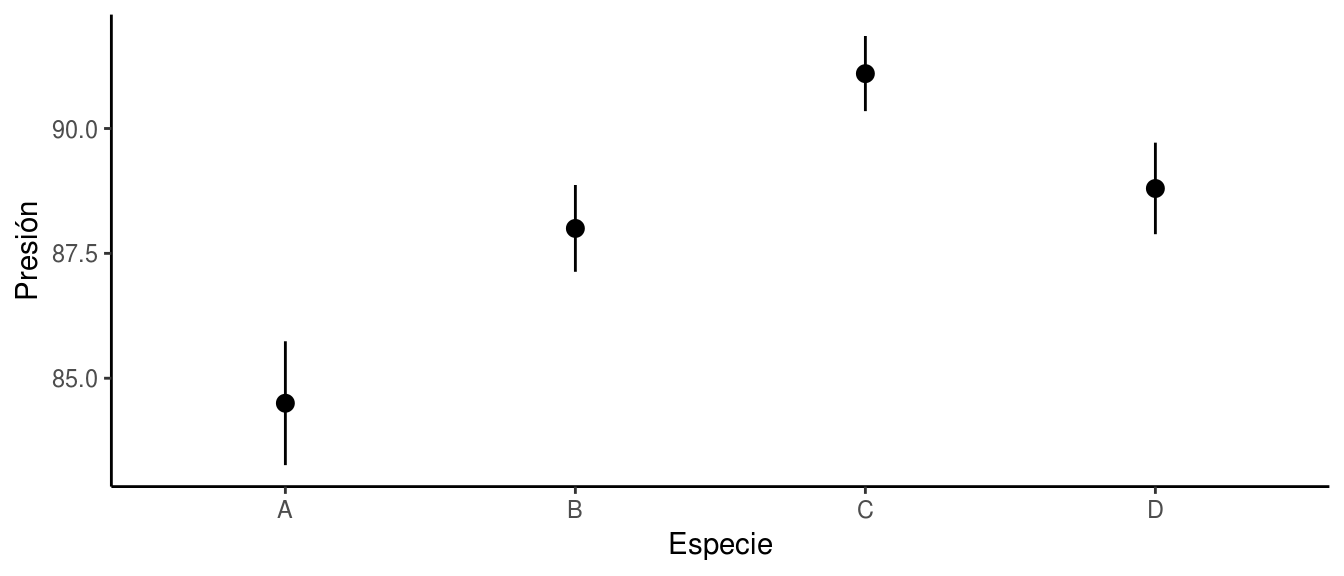
\includegraphics[width=0.75\linewidth]{anova_files/figure-latex/ratas-posteriori-1} \caption{Presion de cuatro especies de ratas. media +- error estándar, n = 10.}\label{fig:ratas-posteriori}
\end{figure}

\textbf{Test de Sheffé}

\begin{verbatim}
## 
## Study: ratas_aov ~ "especie"
## 
## Scheffe Test for presion 
## 
## Mean Square Error  : 9.25 
## 
## especie,  means
## 
##   presion      std  r Min Max
## A    84.5 3.922867 10  79  92
## B    88.0 2.748737 10  84  92
## C    91.1 2.378141 10  87  95
## D    88.8 2.898275 10  85  93
## 
## Alpha: 0.05 ; DF Error: 36 
## Critical Value of F: 2.866266 
## 
## Minimum Significant Difference: 3.988455 
## 
## Means with the same letter are not significantly different.
## 
##   presion groups
## C    91.1      a
## D    88.8      a
## B    88.0     ab
## A    84.5      b
\end{verbatim}

\textbf{Test de Tukey}

\begin{verbatim}
## 
## Study: ratas_aov ~ "especie"
## 
## HSD Test for presion 
## 
## Mean Square Error:  9.25 
## 
## especie,  means
## 
##   presion      std  r Min Max
## A    84.5 3.922867 10  79  92
## B    88.0 2.748737 10  84  92
## C    91.1 2.378141 10  87  95
## D    88.8 2.898275 10  85  93
## 
## Alpha: 0.05 ; DF Error: 36 
## Critical Value of Studentized Range: 3.808798 
## 
## Minimun Significant Difference: 3.663185 
## 
## Treatments with the same letter are not significantly different.
## 
##   presion groups
## C    91.1      a
## D    88.8      a
## B    88.0     ab
## A    84.5      b
\end{verbatim}

\textbf{Polinomios ortogonales}

\begin{longtable}[]{@{}cccccc@{}}
\toprule
\begin{minipage}[b]{0.28\columnwidth}\centering
~\strut
\end{minipage} & \begin{minipage}[b]{0.06\columnwidth}\centering
Df\strut
\end{minipage} & \begin{minipage}[b]{0.10\columnwidth}\centering
Sum Sq\strut
\end{minipage} & \begin{minipage}[b]{0.12\columnwidth}\centering
Mean Sq\strut
\end{minipage} & \begin{minipage}[b]{0.12\columnwidth}\centering
F value\strut
\end{minipage} & \begin{minipage}[b]{0.13\columnwidth}\centering
Pr(\textgreater{}F)\strut
\end{minipage}\tabularnewline
\midrule
\endhead
\begin{minipage}[t]{0.28\columnwidth}\centering
\textbf{especie}\strut
\end{minipage} & \begin{minipage}[t]{0.06\columnwidth}\centering
3\strut
\end{minipage} & \begin{minipage}[t]{0.10\columnwidth}\centering
224.6\strut
\end{minipage} & \begin{minipage}[t]{0.12\columnwidth}\centering
74.87\strut
\end{minipage} & \begin{minipage}[t]{0.12\columnwidth}\centering
8.094\strut
\end{minipage} & \begin{minipage}[t]{0.13\columnwidth}\centering
0.0003005\strut
\end{minipage}\tabularnewline
\begin{minipage}[t]{0.28\columnwidth}\centering
\textbf{especie: A vs C-D}\strut
\end{minipage} & \begin{minipage}[t]{0.06\columnwidth}\centering
1\strut
\end{minipage} & \begin{minipage}[t]{0.10\columnwidth}\centering
198\strut
\end{minipage} & \begin{minipage}[t]{0.12\columnwidth}\centering
198\strut
\end{minipage} & \begin{minipage}[t]{0.12\columnwidth}\centering
21.41\strut
\end{minipage} & \begin{minipage}[t]{0.13\columnwidth}\centering
4.672e-05\strut
\end{minipage}\tabularnewline
\begin{minipage}[t]{0.28\columnwidth}\centering
\textbf{especie: A vs B}\strut
\end{minipage} & \begin{minipage}[t]{0.06\columnwidth}\centering
1\strut
\end{minipage} & \begin{minipage}[t]{0.10\columnwidth}\centering
0.1333\strut
\end{minipage} & \begin{minipage}[t]{0.12\columnwidth}\centering
0.1333\strut
\end{minipage} & \begin{minipage}[t]{0.12\columnwidth}\centering
0.01441\strut
\end{minipage} & \begin{minipage}[t]{0.13\columnwidth}\centering
0.9051\strut
\end{minipage}\tabularnewline
\begin{minipage}[t]{0.28\columnwidth}\centering
\textbf{especie: C vs D}\strut
\end{minipage} & \begin{minipage}[t]{0.06\columnwidth}\centering
1\strut
\end{minipage} & \begin{minipage}[t]{0.10\columnwidth}\centering
26.45\strut
\end{minipage} & \begin{minipage}[t]{0.12\columnwidth}\centering
26.45\strut
\end{minipage} & \begin{minipage}[t]{0.12\columnwidth}\centering
2.859\strut
\end{minipage} & \begin{minipage}[t]{0.13\columnwidth}\centering
0.09948\strut
\end{minipage}\tabularnewline
\begin{minipage}[t]{0.28\columnwidth}\centering
\textbf{Residuals}\strut
\end{minipage} & \begin{minipage}[t]{0.06\columnwidth}\centering
36\strut
\end{minipage} & \begin{minipage}[t]{0.10\columnwidth}\centering
333\strut
\end{minipage} & \begin{minipage}[t]{0.12\columnwidth}\centering
9.25\strut
\end{minipage} & \begin{minipage}[t]{0.12\columnwidth}\centering
NA\strut
\end{minipage} & \begin{minipage}[t]{0.13\columnwidth}\centering
NA\strut
\end{minipage}\tabularnewline
\bottomrule
\end{longtable}

Tabla: Modelo de Análisis de la Varianza Existen diferencias entre A vs
C --D y no existen entre C y D.

\emph{Ejercicio:} Comprobar si los contrastes son ortogonales.

\textbf{Prueba de homogeneidad de varianzas}

\begin{longtable}[]{@{}cccc@{}}
\toprule
\begin{minipage}[b]{0.15\columnwidth}\centering
~\strut
\end{minipage} & \begin{minipage}[b]{0.06\columnwidth}\centering
Df\strut
\end{minipage} & \begin{minipage}[b]{0.12\columnwidth}\centering
F value\strut
\end{minipage} & \begin{minipage}[b]{0.12\columnwidth}\centering
Pr(\textgreater{}F)\strut
\end{minipage}\tabularnewline
\midrule
\endhead
\begin{minipage}[t]{0.15\columnwidth}\centering
\textbf{group}\strut
\end{minipage} & \begin{minipage}[t]{0.06\columnwidth}\centering
3\strut
\end{minipage} & \begin{minipage}[t]{0.12\columnwidth}\centering
0.7086\strut
\end{minipage} & \begin{minipage}[t]{0.12\columnwidth}\centering
0.5532\strut
\end{minipage}\tabularnewline
\begin{minipage}[t]{0.15\columnwidth}\centering
\strut
\end{minipage} & \begin{minipage}[t]{0.06\columnwidth}\centering
36\strut
\end{minipage} & \begin{minipage}[t]{0.12\columnwidth}\centering
NA\strut
\end{minipage} & \begin{minipage}[t]{0.12\columnwidth}\centering
NA\strut
\end{minipage}\tabularnewline
\bottomrule
\end{longtable}

Tabla: Prueba de Levene para homogeneidad de varianzas (centro =
mediana).

\begin{longtable}[]{@{}ccccc@{}}
\toprule
\begin{minipage}[b]{0.19\columnwidth}\centering
~\strut
\end{minipage} & \begin{minipage}[b]{0.11\columnwidth}\centering
Sum Sq\strut
\end{minipage} & \begin{minipage}[b]{0.06\columnwidth}\centering
Df\strut
\end{minipage} & \begin{minipage}[b]{0.12\columnwidth}\centering
F value\strut
\end{minipage} & \begin{minipage}[b]{0.13\columnwidth}\centering
Pr(\textgreater{}F)\strut
\end{minipage}\tabularnewline
\midrule
\endhead
\begin{minipage}[t]{0.19\columnwidth}\centering
\textbf{especie}\strut
\end{minipage} & \begin{minipage}[t]{0.11\columnwidth}\centering
224.6\strut
\end{minipage} & \begin{minipage}[t]{0.06\columnwidth}\centering
3\strut
\end{minipage} & \begin{minipage}[t]{0.12\columnwidth}\centering
8.094\strut
\end{minipage} & \begin{minipage}[t]{0.13\columnwidth}\centering
0.0003005\strut
\end{minipage}\tabularnewline
\begin{minipage}[t]{0.19\columnwidth}\centering
\textbf{Residuals}\strut
\end{minipage} & \begin{minipage}[t]{0.11\columnwidth}\centering
333\strut
\end{minipage} & \begin{minipage}[t]{0.06\columnwidth}\centering
36\strut
\end{minipage} & \begin{minipage}[t]{0.12\columnwidth}\centering
NA\strut
\end{minipage} & \begin{minipage}[t]{0.13\columnwidth}\centering
NA\strut
\end{minipage}\tabularnewline
\bottomrule
\end{longtable}

Tabla: ANOVA (Tipo II)

\textbf{Medias marginales estimadas}

\begin{longtable}[]{@{}cccccc@{}}
\toprule
\begin{minipage}[b]{0.12\columnwidth}\centering
especie\strut
\end{minipage} & \begin{minipage}[b]{0.10\columnwidth}\centering
lsmean\strut
\end{minipage} & \begin{minipage}[b]{0.10\columnwidth}\centering
SE\strut
\end{minipage} & \begin{minipage}[b]{0.06\columnwidth}\centering
df\strut
\end{minipage} & \begin{minipage}[b]{0.13\columnwidth}\centering
lower.CL\strut
\end{minipage} & \begin{minipage}[b]{0.13\columnwidth}\centering
upper.CL\strut
\end{minipage}\tabularnewline
\midrule
\endhead
\begin{minipage}[t]{0.12\columnwidth}\centering
A\strut
\end{minipage} & \begin{minipage}[t]{0.10\columnwidth}\centering
84.5\strut
\end{minipage} & \begin{minipage}[t]{0.10\columnwidth}\centering
0.9618\strut
\end{minipage} & \begin{minipage}[t]{0.06\columnwidth}\centering
36\strut
\end{minipage} & \begin{minipage}[t]{0.13\columnwidth}\centering
82.55\strut
\end{minipage} & \begin{minipage}[t]{0.13\columnwidth}\centering
86.45\strut
\end{minipage}\tabularnewline
\begin{minipage}[t]{0.12\columnwidth}\centering
B\strut
\end{minipage} & \begin{minipage}[t]{0.10\columnwidth}\centering
88\strut
\end{minipage} & \begin{minipage}[t]{0.10\columnwidth}\centering
0.9618\strut
\end{minipage} & \begin{minipage}[t]{0.06\columnwidth}\centering
36\strut
\end{minipage} & \begin{minipage}[t]{0.13\columnwidth}\centering
86.05\strut
\end{minipage} & \begin{minipage}[t]{0.13\columnwidth}\centering
89.95\strut
\end{minipage}\tabularnewline
\begin{minipage}[t]{0.12\columnwidth}\centering
C\strut
\end{minipage} & \begin{minipage}[t]{0.10\columnwidth}\centering
91.1\strut
\end{minipage} & \begin{minipage}[t]{0.10\columnwidth}\centering
0.9618\strut
\end{minipage} & \begin{minipage}[t]{0.06\columnwidth}\centering
36\strut
\end{minipage} & \begin{minipage}[t]{0.13\columnwidth}\centering
89.15\strut
\end{minipage} & \begin{minipage}[t]{0.13\columnwidth}\centering
93.05\strut
\end{minipage}\tabularnewline
\begin{minipage}[t]{0.12\columnwidth}\centering
D\strut
\end{minipage} & \begin{minipage}[t]{0.10\columnwidth}\centering
88.8\strut
\end{minipage} & \begin{minipage}[t]{0.10\columnwidth}\centering
0.9618\strut
\end{minipage} & \begin{minipage}[t]{0.06\columnwidth}\centering
36\strut
\end{minipage} & \begin{minipage}[t]{0.13\columnwidth}\centering
86.85\strut
\end{minipage} & \begin{minipage}[t]{0.13\columnwidth}\centering
90.75\strut
\end{minipage}\tabularnewline
\bottomrule
\end{longtable}

\textbf{Pruebas post hoc}

\begin{longtable}[]{@{}ccccccc@{}}
\toprule
\begin{minipage}[b]{0.16\columnwidth}\centering
Prueba\strut
\end{minipage} & \begin{minipage}[b]{0.12\columnwidth}\centering
contrast\strut
\end{minipage} & \begin{minipage}[b]{0.11\columnwidth}\centering
estimate\strut
\end{minipage} & \begin{minipage}[b]{0.10\columnwidth}\centering
SE\strut
\end{minipage} & \begin{minipage}[b]{0.09\columnwidth}\centering
df\strut
\end{minipage} & \begin{minipage}[b]{0.12\columnwidth}\centering
t.ratio\strut
\end{minipage} & \begin{minipage}[b]{0.13\columnwidth}\centering
p.value\strut
\end{minipage}\tabularnewline
\midrule
\endhead
\begin{minipage}[t]{0.16\columnwidth}\centering
Tukey\strut
\end{minipage} & \begin{minipage}[t]{0.12\columnwidth}\centering
A - B\strut
\end{minipage} & \begin{minipage}[t]{0.11\columnwidth}\centering
-3.5\strut
\end{minipage} & \begin{minipage}[t]{0.10\columnwidth}\centering
1.4\strut
\end{minipage} & \begin{minipage}[t]{0.09\columnwidth}\centering
36\strut
\end{minipage} & \begin{minipage}[t]{0.12\columnwidth}\centering
-2.57\strut
\end{minipage} & \begin{minipage}[t]{0.13\columnwidth}\centering
0.06553\strut
\end{minipage}\tabularnewline
\begin{minipage}[t]{0.16\columnwidth}\centering
\textbf{Tukey}\strut
\end{minipage} & \begin{minipage}[t]{0.12\columnwidth}\centering
\textbf{A - C}\strut
\end{minipage} & \begin{minipage}[t]{0.11\columnwidth}\centering
\textbf{-6.6}\strut
\end{minipage} & \begin{minipage}[t]{0.10\columnwidth}\centering
\textbf{1.4}\strut
\end{minipage} & \begin{minipage}[t]{0.09\columnwidth}\centering
\textbf{36}\strut
\end{minipage} & \begin{minipage}[t]{0.12\columnwidth}\centering
\textbf{-4.85}\strut
\end{minipage} & \begin{minipage}[t]{0.13\columnwidth}\centering
\textbf{0.00013}\strut
\end{minipage}\tabularnewline
\begin{minipage}[t]{0.16\columnwidth}\centering
\textbf{Tukey}\strut
\end{minipage} & \begin{minipage}[t]{0.12\columnwidth}\centering
\textbf{A - D}\strut
\end{minipage} & \begin{minipage}[t]{0.11\columnwidth}\centering
\textbf{-4.3}\strut
\end{minipage} & \begin{minipage}[t]{0.10\columnwidth}\centering
\textbf{1.4}\strut
\end{minipage} & \begin{minipage}[t]{0.09\columnwidth}\centering
\textbf{36}\strut
\end{minipage} & \begin{minipage}[t]{0.12\columnwidth}\centering
\textbf{-3.16}\strut
\end{minipage} & \begin{minipage}[t]{0.13\columnwidth}\centering
\textbf{0.01606}\strut
\end{minipage}\tabularnewline
\begin{minipage}[t]{0.16\columnwidth}\centering
Tukey\strut
\end{minipage} & \begin{minipage}[t]{0.12\columnwidth}\centering
B - C\strut
\end{minipage} & \begin{minipage}[t]{0.11\columnwidth}\centering
-3.1\strut
\end{minipage} & \begin{minipage}[t]{0.10\columnwidth}\centering
1.4\strut
\end{minipage} & \begin{minipage}[t]{0.09\columnwidth}\centering
36\strut
\end{minipage} & \begin{minipage}[t]{0.12\columnwidth}\centering
-2.28\strut
\end{minipage} & \begin{minipage}[t]{0.13\columnwidth}\centering
0.12197\strut
\end{minipage}\tabularnewline
\begin{minipage}[t]{0.16\columnwidth}\centering
Tukey\strut
\end{minipage} & \begin{minipage}[t]{0.12\columnwidth}\centering
B - D\strut
\end{minipage} & \begin{minipage}[t]{0.11\columnwidth}\centering
-0.8\strut
\end{minipage} & \begin{minipage}[t]{0.10\columnwidth}\centering
1.4\strut
\end{minipage} & \begin{minipage}[t]{0.09\columnwidth}\centering
36\strut
\end{minipage} & \begin{minipage}[t]{0.12\columnwidth}\centering
-0.59\strut
\end{minipage} & \begin{minipage}[t]{0.13\columnwidth}\centering
0.93501\strut
\end{minipage}\tabularnewline
\begin{minipage}[t]{0.16\columnwidth}\centering
Tukey\strut
\end{minipage} & \begin{minipage}[t]{0.12\columnwidth}\centering
C - D\strut
\end{minipage} & \begin{minipage}[t]{0.11\columnwidth}\centering
2.3\strut
\end{minipage} & \begin{minipage}[t]{0.10\columnwidth}\centering
1.4\strut
\end{minipage} & \begin{minipage}[t]{0.09\columnwidth}\centering
36\strut
\end{minipage} & \begin{minipage}[t]{0.12\columnwidth}\centering
1.69\strut
\end{minipage} & \begin{minipage}[t]{0.13\columnwidth}\centering
0.34314\strut
\end{minipage}\tabularnewline
\begin{minipage}[t]{0.16\columnwidth}\centering
Bonferroni\strut
\end{minipage} & \begin{minipage}[t]{0.12\columnwidth}\centering
A - B\strut
\end{minipage} & \begin{minipage}[t]{0.11\columnwidth}\centering
-3.5\strut
\end{minipage} & \begin{minipage}[t]{0.10\columnwidth}\centering
1.4\strut
\end{minipage} & \begin{minipage}[t]{0.09\columnwidth}\centering
36\strut
\end{minipage} & \begin{minipage}[t]{0.12\columnwidth}\centering
-2.57\strut
\end{minipage} & \begin{minipage}[t]{0.13\columnwidth}\centering
0.08604\strut
\end{minipage}\tabularnewline
\begin{minipage}[t]{0.16\columnwidth}\centering
\textbf{Bonferroni}\strut
\end{minipage} & \begin{minipage}[t]{0.12\columnwidth}\centering
\textbf{A - C}\strut
\end{minipage} & \begin{minipage}[t]{0.11\columnwidth}\centering
\textbf{-6.6}\strut
\end{minipage} & \begin{minipage}[t]{0.10\columnwidth}\centering
\textbf{1.4}\strut
\end{minipage} & \begin{minipage}[t]{0.09\columnwidth}\centering
\textbf{36}\strut
\end{minipage} & \begin{minipage}[t]{0.12\columnwidth}\centering
\textbf{-4.85}\strut
\end{minipage} & \begin{minipage}[t]{0.13\columnwidth}\centering
\textbf{0.00014}\strut
\end{minipage}\tabularnewline
\begin{minipage}[t]{0.16\columnwidth}\centering
\textbf{Bonferroni}\strut
\end{minipage} & \begin{minipage}[t]{0.12\columnwidth}\centering
\textbf{A - D}\strut
\end{minipage} & \begin{minipage}[t]{0.11\columnwidth}\centering
\textbf{-4.3}\strut
\end{minipage} & \begin{minipage}[t]{0.10\columnwidth}\centering
\textbf{1.4}\strut
\end{minipage} & \begin{minipage}[t]{0.09\columnwidth}\centering
\textbf{36}\strut
\end{minipage} & \begin{minipage}[t]{0.12\columnwidth}\centering
\textbf{-3.16}\strut
\end{minipage} & \begin{minipage}[t]{0.13\columnwidth}\centering
\textbf{0.01908}\strut
\end{minipage}\tabularnewline
\begin{minipage}[t]{0.16\columnwidth}\centering
Bonferroni\strut
\end{minipage} & \begin{minipage}[t]{0.12\columnwidth}\centering
B - C\strut
\end{minipage} & \begin{minipage}[t]{0.11\columnwidth}\centering
-3.1\strut
\end{minipage} & \begin{minipage}[t]{0.10\columnwidth}\centering
1.4\strut
\end{minipage} & \begin{minipage}[t]{0.09\columnwidth}\centering
36\strut
\end{minipage} & \begin{minipage}[t]{0.12\columnwidth}\centering
-2.28\strut
\end{minipage} & \begin{minipage}[t]{0.13\columnwidth}\centering
0.17213\strut
\end{minipage}\tabularnewline
\begin{minipage}[t]{0.16\columnwidth}\centering
Bonferroni\strut
\end{minipage} & \begin{minipage}[t]{0.12\columnwidth}\centering
B - D\strut
\end{minipage} & \begin{minipage}[t]{0.11\columnwidth}\centering
-0.8\strut
\end{minipage} & \begin{minipage}[t]{0.10\columnwidth}\centering
1.4\strut
\end{minipage} & \begin{minipage}[t]{0.09\columnwidth}\centering
36\strut
\end{minipage} & \begin{minipage}[t]{0.12\columnwidth}\centering
-0.59\strut
\end{minipage} & \begin{minipage}[t]{0.13\columnwidth}\centering
1\strut
\end{minipage}\tabularnewline
\begin{minipage}[t]{0.16\columnwidth}\centering
Bonferroni\strut
\end{minipage} & \begin{minipage}[t]{0.12\columnwidth}\centering
C - D\strut
\end{minipage} & \begin{minipage}[t]{0.11\columnwidth}\centering
2.3\strut
\end{minipage} & \begin{minipage}[t]{0.10\columnwidth}\centering
1.4\strut
\end{minipage} & \begin{minipage}[t]{0.09\columnwidth}\centering
36\strut
\end{minipage} & \begin{minipage}[t]{0.12\columnwidth}\centering
1.69\strut
\end{minipage} & \begin{minipage}[t]{0.13\columnwidth}\centering
0.59688\strut
\end{minipage}\tabularnewline
\begin{minipage}[t]{0.16\columnwidth}\centering
\textbf{LSD}\strut
\end{minipage} & \begin{minipage}[t]{0.12\columnwidth}\centering
\textbf{A - B}\strut
\end{minipage} & \begin{minipage}[t]{0.11\columnwidth}\centering
\textbf{-3.5}\strut
\end{minipage} & \begin{minipage}[t]{0.10\columnwidth}\centering
\textbf{1.4}\strut
\end{minipage} & \begin{minipage}[t]{0.09\columnwidth}\centering
\textbf{36}\strut
\end{minipage} & \begin{minipage}[t]{0.12\columnwidth}\centering
\textbf{-2.57}\strut
\end{minipage} & \begin{minipage}[t]{0.13\columnwidth}\centering
\textbf{0.01434}\strut
\end{minipage}\tabularnewline
\begin{minipage}[t]{0.16\columnwidth}\centering
\textbf{LSD}\strut
\end{minipage} & \begin{minipage}[t]{0.12\columnwidth}\centering
\textbf{A - C}\strut
\end{minipage} & \begin{minipage}[t]{0.11\columnwidth}\centering
\textbf{-6.6}\strut
\end{minipage} & \begin{minipage}[t]{0.10\columnwidth}\centering
\textbf{1.4}\strut
\end{minipage} & \begin{minipage}[t]{0.09\columnwidth}\centering
\textbf{36}\strut
\end{minipage} & \begin{minipage}[t]{0.12\columnwidth}\centering
\textbf{-4.85}\strut
\end{minipage} & \begin{minipage}[t]{0.13\columnwidth}\centering
\textbf{2e-05}\strut
\end{minipage}\tabularnewline
\begin{minipage}[t]{0.16\columnwidth}\centering
\textbf{LSD}\strut
\end{minipage} & \begin{minipage}[t]{0.12\columnwidth}\centering
\textbf{A - D}\strut
\end{minipage} & \begin{minipage}[t]{0.11\columnwidth}\centering
\textbf{-4.3}\strut
\end{minipage} & \begin{minipage}[t]{0.10\columnwidth}\centering
\textbf{1.4}\strut
\end{minipage} & \begin{minipage}[t]{0.09\columnwidth}\centering
\textbf{36}\strut
\end{minipage} & \begin{minipage}[t]{0.12\columnwidth}\centering
\textbf{-3.16}\strut
\end{minipage} & \begin{minipage}[t]{0.13\columnwidth}\centering
\textbf{0.00318}\strut
\end{minipage}\tabularnewline
\begin{minipage}[t]{0.16\columnwidth}\centering
\textbf{LSD}\strut
\end{minipage} & \begin{minipage}[t]{0.12\columnwidth}\centering
\textbf{B - C}\strut
\end{minipage} & \begin{minipage}[t]{0.11\columnwidth}\centering
\textbf{-3.1}\strut
\end{minipage} & \begin{minipage}[t]{0.10\columnwidth}\centering
\textbf{1.4}\strut
\end{minipage} & \begin{minipage}[t]{0.09\columnwidth}\centering
\textbf{36}\strut
\end{minipage} & \begin{minipage}[t]{0.12\columnwidth}\centering
\textbf{-2.28}\strut
\end{minipage} & \begin{minipage}[t]{0.13\columnwidth}\centering
\textbf{0.02869}\strut
\end{minipage}\tabularnewline
\begin{minipage}[t]{0.16\columnwidth}\centering
LSD\strut
\end{minipage} & \begin{minipage}[t]{0.12\columnwidth}\centering
B - D\strut
\end{minipage} & \begin{minipage}[t]{0.11\columnwidth}\centering
-0.8\strut
\end{minipage} & \begin{minipage}[t]{0.10\columnwidth}\centering
1.4\strut
\end{minipage} & \begin{minipage}[t]{0.09\columnwidth}\centering
36\strut
\end{minipage} & \begin{minipage}[t]{0.12\columnwidth}\centering
-0.59\strut
\end{minipage} & \begin{minipage}[t]{0.13\columnwidth}\centering
0.56009\strut
\end{minipage}\tabularnewline
\begin{minipage}[t]{0.16\columnwidth}\centering
LSD\strut
\end{minipage} & \begin{minipage}[t]{0.12\columnwidth}\centering
C - D\strut
\end{minipage} & \begin{minipage}[t]{0.11\columnwidth}\centering
2.3\strut
\end{minipage} & \begin{minipage}[t]{0.10\columnwidth}\centering
1.4\strut
\end{minipage} & \begin{minipage}[t]{0.09\columnwidth}\centering
36\strut
\end{minipage} & \begin{minipage}[t]{0.12\columnwidth}\centering
1.69\strut
\end{minipage} & \begin{minipage}[t]{0.13\columnwidth}\centering
0.09948\strut
\end{minipage}\tabularnewline
\begin{minipage}[t]{0.16\columnwidth}\centering
Scheffe\strut
\end{minipage} & \begin{minipage}[t]{0.12\columnwidth}\centering
A - B\strut
\end{minipage} & \begin{minipage}[t]{0.11\columnwidth}\centering
-3.5\strut
\end{minipage} & \begin{minipage}[t]{0.10\columnwidth}\centering
NA\strut
\end{minipage} & \begin{minipage}[t]{0.09\columnwidth}\centering
NA\strut
\end{minipage} & \begin{minipage}[t]{0.12\columnwidth}\centering
NA\strut
\end{minipage} & \begin{minipage}[t]{0.13\columnwidth}\centering
0.1041\strut
\end{minipage}\tabularnewline
\begin{minipage}[t]{0.16\columnwidth}\centering
\textbf{Scheffe}\strut
\end{minipage} & \begin{minipage}[t]{0.12\columnwidth}\centering
\textbf{A - C}\strut
\end{minipage} & \begin{minipage}[t]{0.11\columnwidth}\centering
\textbf{-6.6}\strut
\end{minipage} & \begin{minipage}[t]{0.10\columnwidth}\centering
NA\strut
\end{minipage} & \begin{minipage}[t]{0.09\columnwidth}\centering
NA\strut
\end{minipage} & \begin{minipage}[t]{0.12\columnwidth}\centering
NA\strut
\end{minipage} & \begin{minipage}[t]{0.13\columnwidth}\centering
\textbf{4e-04}\strut
\end{minipage}\tabularnewline
\begin{minipage}[t]{0.16\columnwidth}\centering
\textbf{Scheffe}\strut
\end{minipage} & \begin{minipage}[t]{0.12\columnwidth}\centering
\textbf{A - D}\strut
\end{minipage} & \begin{minipage}[t]{0.11\columnwidth}\centering
\textbf{-4.3}\strut
\end{minipage} & \begin{minipage}[t]{0.10\columnwidth}\centering
NA\strut
\end{minipage} & \begin{minipage}[t]{0.09\columnwidth}\centering
NA\strut
\end{minipage} & \begin{minipage}[t]{0.12\columnwidth}\centering
NA\strut
\end{minipage} & \begin{minipage}[t]{0.13\columnwidth}\centering
\textbf{0.0301}\strut
\end{minipage}\tabularnewline
\begin{minipage}[t]{0.16\columnwidth}\centering
Scheffe\strut
\end{minipage} & \begin{minipage}[t]{0.12\columnwidth}\centering
B - C\strut
\end{minipage} & \begin{minipage}[t]{0.11\columnwidth}\centering
-3.1\strut
\end{minipage} & \begin{minipage}[t]{0.10\columnwidth}\centering
NA\strut
\end{minipage} & \begin{minipage}[t]{0.09\columnwidth}\centering
NA\strut
\end{minipage} & \begin{minipage}[t]{0.12\columnwidth}\centering
NA\strut
\end{minipage} & \begin{minipage}[t]{0.13\columnwidth}\centering
0.1779\strut
\end{minipage}\tabularnewline
\begin{minipage}[t]{0.16\columnwidth}\centering
Scheffe\strut
\end{minipage} & \begin{minipage}[t]{0.12\columnwidth}\centering
B - D\strut
\end{minipage} & \begin{minipage}[t]{0.11\columnwidth}\centering
-0.8\strut
\end{minipage} & \begin{minipage}[t]{0.10\columnwidth}\centering
NA\strut
\end{minipage} & \begin{minipage}[t]{0.09\columnwidth}\centering
NA\strut
\end{minipage} & \begin{minipage}[t]{0.12\columnwidth}\centering
NA\strut
\end{minipage} & \begin{minipage}[t]{0.13\columnwidth}\centering
0.9506\strut
\end{minipage}\tabularnewline
\begin{minipage}[t]{0.16\columnwidth}\centering
Scheffe\strut
\end{minipage} & \begin{minipage}[t]{0.12\columnwidth}\centering
C - D\strut
\end{minipage} & \begin{minipage}[t]{0.11\columnwidth}\centering
2.3\strut
\end{minipage} & \begin{minipage}[t]{0.10\columnwidth}\centering
NA\strut
\end{minipage} & \begin{minipage}[t]{0.09\columnwidth}\centering
NA\strut
\end{minipage} & \begin{minipage}[t]{0.12\columnwidth}\centering
NA\strut
\end{minipage} & \begin{minipage}[t]{0.13\columnwidth}\centering
0.4253\strut
\end{minipage}\tabularnewline
\bottomrule
\end{longtable}

\hypertarget{planificacion-del-tamano-muestral}{%
\section{Planificación Del Tamaño
Muestral}\label{planificacion-del-tamano-muestral}}

\textbf{Diseño De Estudios De ANOVA}

La planificación de los tamaños muestrales es una parte integral del
diseño en un estudio de ANOVA. Se asumirá que todos los niveles del
factor tienen el mismo tamaño muestral

\hypertarget{potencia-de-la-prueba-f}{%
\subsection{Potencia De La Prueba F}\label{potencia-de-la-prueba-f}}

La potencia de la prueba \(F\) es la probabilidad de rechazar \(H_{0}\)
cuando \(H_{0}\) es falsa, o también se puede pensar como la
probabilidad de no rechazar \(H_{a}\) cuando \(H_{a}\) es cierta.
Específicamente la potencia está dada por la siguiente expresión:

\[
P = P\left( F^{*} > F_{\left( \alpha;I - 1,N - I \right)}\left| \phi \right.\  \right)
\]

donde \(\mathbf{\phi}\) es un parámetro de no-centralidad, que es una
medida de cuan distintas son las \(\mu_i\):

\[
\phi = \frac{1}{\sigma}\sqrt{\frac{\sum_{}^{}{n_{i}\left( \mu_{i} - \mu_{\bullet} \right)^{2}}}{I}}
\]

y

\[
\mu_{\bullet} = \frac{\sum_{}^{}{n_{i}\mu_{i}}}{N}
\]

Cuando todos los tamaños muestrales son iguales, el parámetro ϕ es:

\[
\phi = \frac{1}{\sigma}\sqrt{\frac{n\sum_{}^{}\left( \mu_{i} - \mu_{\bullet} \right)^{2}}{I}}\text{con}\ n = n_{i}
\]

donde:

\[
\mu_{} = \frac{\sum_{}^{}\mu_{i}}{I}
\]

Para determinar la potencia, se necesita utilizar la distribución F
no-centrada, dado que ésta es la distribución muestral de \(F^{*}\)
cuando \(H_{a}\) es cierta. Los cálculos son bastantes complejos, pero
se han preparado gráficos que permiten determinar la potencia
relativamente fácil. Estos son los gráficos de Pearson-Hartley de la
potencia de la prueba \(F\). La curva a utilizar depende del número de
niveles del factor, del tamaño muestral y del nivel de significación
empleado en la regla de decisión. Estos gráficos se usan de la siguiente
forma:

Cada página se refiere a diferentes \(\nu_{1}\), los grados de libertad
del numerador de \(F^{*}\). Para el modelo de ANOVA \(\nu_{1} = I1\).

Dos niveles de significación, indicados por \(\alpha\), son usados en
los gráficos, \(\alpha = 0.05\) y \(\alpha = 0.01\). Hay dos escalas de
\(X\), dependiendo de cual es el nivel de significación empleado. De
esta forma, el grupo de curvas de la izquierda corresponde a
\(\alpha = 0.05\) y el de la derecha a \(\alpha = 0.01\).

Hay curvas separadas para diferentes valores de \(\nu_{2}\), los grados
de libertad del denominador de \(F^{*}\). Para el modelo de ANOVA
\(\nu_{2} = NI\). Las curvas son indicadas de acuerdo al valor de
\(\nu_{2}\), en la parte superior del gráfico. Dado que sólo son usados
en la tabla valores seleccionados de \(\nu_{2}\), es necesario
interpolar para valores intermedios de \(\nu_{2}\)

La escala de \(X\) representa a \(\phi\), el parámetro no-central.

La escala de \(Y\) da la potencia \(1 - \beta\), donde \(\beta\) es la
probabilidad de cometer el error de tipo II.

\textbf{Ejemplo 3}.- Consideremos el caso donde \(\nu_{1} = 2\),
\(\nu_{2} = 10\), \(\phi = 10\) y \(\alpha = 0.05\). Si buscamos en la
tabla la potencia es \(1 - \beta = 0.983\) aproximadamente.

Una forma alternativa para determinar la potencia es especificar la
mínima diferencia que se desea detectar entre las medias de las dos
poblaciones más diferentes. Designaremos a esta diferencia mínima
detectable \(\delta\), calculamos entonces:

\[
\phi = \sqrt{\frac{n\delta^{2}}{2IS^{2}}}
\]

\textbf{Ejemplo 4}.- Supongamos que especificamos que trabajaremos con
\(n = 10\), y que deseamos detectar, entre cuatro tratamientos,
diferencias entre las medias de al menos 4 unidades. De un estudio
piloto se sabe que \(S^{2} = 7.5888\). Trabajamos con \(\alpha = 0.05\).

\(I\  = \ 4\nu_{1} = 3\) \(n = 10\) \(\nu_{2} = 36\) \(\delta = 4.0\)
\(S^{2} = 7.5888\)

\[
\begin{aligned}
\phi &= \sqrt{\frac{n\delta^{2}}{2IS^{2}}}\\
\phi &= \sqrt{\frac{10\left( 4.0 \right)^{2}}{2\left( 4 \right)\left( 7.5888 \right)}}\\
\phi &= \sqrt{2.6355}\\
\phi &= 1.62
\end{aligned}
\]

En la tabla obtenemos una potencia igual a \(0.72\); lo que implica una
probabilidad de cometer el error de tipo II del \(28\%\).

Si bien es deseable estimar la potencia antes de realizar el ANOVA, es
útil, también, preguntarse con que potencia se ha realizado un ANOVA.
Esto es especialmente interesante si la \(H_{0}\) no se ha rechazado,
pues entonces es deseable saber cuan bien la prueba detecta las
diferencias entre las medias de la población.

Calculamos \(\phi\), de la siguiente forma:

\[
\phi = \sqrt{\frac{\left( I - 1 \right)\left( CM_E - S^{2} \right)}{IS^{2}}}
\]

\textbf{Ejemplo 5.}- Los datos de la tabla corresponden a una muestra
recogida de tres poblaciones de aves geográficamente aisladas. Se midió
la longitud del pico con una precisión de un décimo de mm; obteniéndose
los siguientes datos:

\begin{longtable}[]{@{}lll@{}}
\toprule
Población & &\tabularnewline
\midrule
\endhead
A & B & C\tabularnewline
4.2 & 3.8 & 3.0\tabularnewline
3.3 & 4.1 & 3.5\tabularnewline
2.8 & 5.0 & 4.5\tabularnewline
4.3 & 4.6 & 4.4\tabularnewline
3.7 & 5.1 &\tabularnewline
4.5 & &\tabularnewline
3.6 & &\tabularnewline
\bottomrule
\end{longtable}

\[
\begin{aligned}
H_{0}&:\ u_{A} = u_{B} = u_{C}\\
H_{a}&:\ \text{No todas las medias de las poblaciones son iguales.}
\end{aligned}
\]

\begin{longtable}[]{@{}lllllll@{}}
\toprule
Fte. de Variación & SC & GL & CM & F & P & VC\tabularnewline
\midrule
\endhead
Entre Dentro & 1.7977143 5.0322857 & 2 13 & 0.8988571 0.3870989 & 2.322
& 0.137322 & 3.806\tabularnewline
Total & 6.83 & 15 & & & &\tabularnewline
\bottomrule
\end{longtable}

No rechazamos \(H_{0}\) con \(p > 0.05\)

\[
\phi = \sqrt{\frac{\left( I - 1 \right)\left( CM_E - S^{2} \right)}{IS^{2}}} = \sqrt{\frac{\left( 3 - 1 \right)\left( 0.898871 - 0.387098 \right)}{3\left( 0.3870989 \right)}} = 0.9388053
\]

Consultando la tabla la Potencia es 0.25; por lo cual la probabilidad de
cometer error de tipo II es aproximadamente de 0.75.

\begin{itemize}
\item
  Se puede observar que grandes valores de \(\phi\) están asociados con
  grandes potencias, de las ecuaciones vistas anteriormente se ve que
  \(\phi\) se incrementa con:
\item
  incremento del tamaño muestral;
\item
  incremento entre las diferencias de las medias de las poblaciones
  (medida ya sea por \(CM_E\) , o por
  \(\sum_{}^{}\left( \mu_{i} - \mu_{} \right)^{2}\) o por la mínima
  diferencia detectable);
\item
  un bajo número de niveles del factor o de tratamientos;
\item
  una disminución de la variabilidad dentro de las poblaciones,
  \(\sigma^{2}\), estimada por \(S^{2}\) o el \(CM_D\).
\end{itemize}

\textbf{Ejemplo 6.-} Veamos qué pasa con el experimento anterior al
aumentar el tamaño de la muestra.

\begin{longtable}[]{@{}lllllll@{}}
\toprule
POBLACIÓN & & & & & &\tabularnewline
\midrule
\endhead
A & B & C & & & &\tabularnewline
3.9 & 4.6 & 3.7 & & & &\tabularnewline
3.5 & 4.1 & 4.2 & & & &\tabularnewline
4.1 & 4.5 & 3.6 & & & &\tabularnewline
4.4 & 4.4 & 4.0 & & & &\tabularnewline
4.4 & 3.7 & 3.3 & & & &\tabularnewline
4.6 & 4.6 & 3.5 & & & &\tabularnewline
3.3 & 3.9 & 4.0 & & & &\tabularnewline
3.9 & 4.6 & 4.4 & & & &\tabularnewline
4.4 & 4.5 & 3.5 & & & &\tabularnewline
3.6 & 3.7 & 4.1 & & & &\tabularnewline
3.7 & 4.1 & 3.9 & & & &\tabularnewline
3.4 & 4.2 & 4.3 & & & &\tabularnewline
\bottomrule
\end{longtable}

\begin{longtable}[]{@{}lllllll@{}}
\toprule
Fte. de Variación & SC & GL & CM & F & p & VC\tabularnewline
\midrule
\endhead
Entre & 0.9433318 & 2 & 0.4716659 & 3.179 & 0.05458498 &
3.285\tabularnewline
Dentro & 4.89465511 & 33 & 0.14832288 & & &\tabularnewline
Total & 5.8379869 & 35 & & & &\tabularnewline
\bottomrule
\end{longtable}

\[
\mathbf{\phi}\  \approx \ 1.21
\]

La potencia es entonces 0.4

Para el uso de las tablas vistas anteriormente se hace necesario la
realización de un experimento. Pero existen tablas que proporcionan los
tamaños muestrales adecuados directamente. Este método es aplicable
cuando todos los niveles del factor tienen el mismo tamaño muestral,
esto es \(n = n_{i}\).

La planificación del tamaño de la muestra usando estas tablas se hace en
términos del parámetro de no-centralidad, para tamaños muestrales
iguales. Sin embargo, en lugar de requerir una especificación directa de
los niveles de \(u_{i}\) para los cuales es importante controlar la
probabilidad de cometer el error de tipo II; esta tabla sólo requiere
una especificación del rango mínimo de las medias de los niveles del
factor para los cuales es importante detectar diferencias entre los
\(u_{i}\), con alta probabilidad. Este rango mínimo se indica
\(\Delta\):

\[
\Delta = max\left( u_{i} \right)min\left( u_{i} \right)
\]

Las siguientes especificaciones son necesarias para hacer uso de la
tabla:

\begin{enumerate}
\def\labelenumi{\arabic{enumi}.}
\item
  El nivel de significación \(\alpha\)
\item
  La magnitud del rango mínimo \(\Delta\) de los \(u_{i}\), la cual es
  importante detectar con alta probabilidad. La magnitud de \(\sigma\),
  la desviación estándar de \(Y\), debe también ser especificada para
  entrar en la tabla en términos del cociente: \(\frac{\Delta}{\sigma}\)
\item
  El nivel de \(\beta\). Entrar en la tabla en términos de
  \(1 - \beta\).
\end{enumerate}

Cuando se usa la tabla están disponibles cuatro niveles de \(\alpha\
(0.2;0.1;0.05\ y\ 0.01)\). También hay cuatro niveles de β a través de
la potencia. La tabla provee tamaños muestrales para estudios
\(\text{de}\ I = 2,\ldots,10\) niveles del factor o tratamientos.

\textbf{Ejemplo 7.}- 1) Supongamos que se quiere con un rango mínimo
\(\Delta = 3\), para comparar cuatro tratamientos. Se sabe por estudios
anteriores que \(\sigma\) es aproximadamente igual a 2. Los niveles para
controlar los errores son:

\[
\alpha = 0.05\ \beta = 0.10\ o\ P = 1 - \beta = 0.90
\]

Entramos a la tabla para \(\frac{\Delta}{\sigma} = \frac{3}{2} = 1.5\);
\(\alpha = 0.05\); \(1 - \beta = 0.9\) e \(I = 4\). Encontramos que
\(n = 14\).

Especificación de \(\frac{\Delta}{\sigma}\) directa: El rango mínimo
también se puede especificar en términos de unidades de desviación
estándar.

\[
\frac{\Delta}{\sigma} = \frac{k\sigma}{\sigma} = k
\]

En nuestro ejemplo supongamos que el rango de las medias es k = 2 o más.
Supongamos que las otras especificaciones son:

\[
\alpha = 0.01\ \beta = 0.05\ o\ 1 - \beta = 0.95
\]

En la tabla encontramos que \(n = 9\).

\begin{enumerate}
\def\labelenumi{\arabic{enumi})}
\setcounter{enumi}{1}
\tightlist
\item
  En el ejemplo se hace necesario incrementar el tamaño de la muestra.
  Para ello nos preguntamos cuál es el tamaño de muestra necesario para,
  trabajando con \(\alpha = 0.05\), tener una potencia de \(0.80\) para
  detectar diferencias tan pequeñas como \(0.7\). Suponemos que
  \(S^{2} = 0.3870989\) es una buena estimación de \(\sigma^{2}\).
\end{enumerate}

Entramos a la tabla para
\(\frac{\Delta}{\sigma} = \frac{0.6}{\sqrt{0.387089}} \approx 1\);
\(\alpha = 0.05\); \(1 - \beta = 0.8\) e \(I = 3\)

Encontramos que \(n = 21\).

\hypertarget{modelo-ii-de-anova-niveles-del-factor-aleatorios}{%
\section{Modelo II De ANOVA: Niveles Del Factor
Aleatorios}\label{modelo-ii-de-anova-niveles-del-factor-aleatorios}}

Existen situaciones en las cuales los niveles del factor o los
tratamientos empleados no tienen un interés en sí mismos, pero
constituyen una muestra de la población. El Modelo II de ANOVA está
diseñado para este tipo de situaciones.

\hypertarget{modelo-aleatorio-de-medias-de-celdas.}{%
\subsection{Modelo Aleatorio de Medias de
Celdas.}\label{modelo-aleatorio-de-medias-de-celdas.}}

El modelo II de ANOVA para un factor es:

\[
Y_{ij}\  = \ u_{i}\  + \ \varepsilon_{ij}
\]

donde

\(u_{i}\) son variables independientes
\(\sim N\left( \mu_{\bullet},\sigma_{\mu}^{2} \right)\)

\(\varepsilon{ij}\) son variables independientes
\(\sim N\left( 0,\sigma^{2} \right)\)

\(u_{i}\) y \(\varepsilon_{ij}\) son variables aleatorias independientes

\[
i = 1,\ 2,\ldots,\ I;\ j = 1,\ 2,\ \ldots,\ n_{i}
\]

\hypertarget{caracteristicas-importantes-del-modelo-1}{%
\subsection{Características importantes del
Modelo}\label{caracteristicas-importantes-del-modelo-1}}

El valor esperado de una observación \(Y_{ij}\) es:

\[
E(Y_{ij}) = u_{\bullet}
\]

esto se debe a que:

\[
\begin{aligned}
E\left( Y_{ij} \right)& = E\left( u_{\bullet}\  \right) + \ E\left( \varepsilon_{ij} \right) \\
& = \ u_{\bullet}\ \  + \ 0 \\
& = \ u_{\bullet} \\
\end{aligned}
\]

La varianza de \(Y_{ij}\), que se indica \(\sigma_{Y}^{2}\), es:

\[
\text{Var}\left( Y_{ij} \right) = \sigma_{Y}^{2} = \sigma_{\mu}^{2} + \sigma^{2}
\]

A causa de que la varianza de Y en este modelo es la suma de dos
componentes, este modelo se llama, algunas veces, un modelo de
componentes de la varianza.

Los \(Y_{ij}\) están normalmente distribuidos pues son una combinación
lineal de variables independientes, \(u_{i}\) y \(\varepsilon_{ij}\),
distribuidas normalmente

Las \(Y_{ij}\) para el modelo aleatorio son sólo independientes si
pertenecen a diferentes tratamientos o niveles del factor. Se puede
demostrar que la covarianza para cualesquiera dos observaciones
\(Y_{ij}\) e \(Y_{{ij}'}\), para el mismo nivel i con un modelo II es:

\[
Cov(Y_{ij},\ Y_{ij'}) = \sigma_{Y}^{2}\; \forall\ j \neq  j
\]

El modelo II supone que la covarianza entre cualesquiera dos
observaciones para el mismo nivel del factor es constante para todos los
niveles del factor.

Una vez que los niveles del factor han sido seleccionados, el modelo II
asume que dos observaciones cualesquiera para el mismo nivel del factor
son independientes pues la media del nivel del factor µi es entonces
fijada y las dos observaciones difieren sólo por los términos del error
\(\varepsilon_{ij}\).

\hypertarget{cuestiones-de-interes}{%
\subsection{Cuestiones de Interés}\label{cuestiones-de-interes}}

Cuando el modelo aleatorio es apropiado, uno no está particularmente
interesado en inferencias sobre un \(u_{i}\) particular incluido en el
estudio, ya sea si es grande o pequeño, pero sí en inferencias acerca de
la población completa de \(mu_{i}\). Específicamente, el interés a
menudo se centra sobre la media de los \(mu_{i}\), \(u_{}\), y en la
variabilidad de los \(mu_{i}\) medida por \(\sigma_{\mu}^{2}\).

Dado que \(\sigma_{\mu}^{2}\) es una medida directa de la variabilidad
de los \(mu_{i}\), el efecto de esa variabilidad, a menudo, es medido
por el cociente:

\[
\frac{\sigma_{\mu}^{2}}{\sigma_{\mu}^{2} + \sigma^{2}}
\]

\begin{enumerate}
\def\labelenumi{\arabic{enumi}.}
\item
  El cociente toma valores entre \(0\ (\sigma^{2} = \infty)\) y \(1\
  (\sigma^{2} = 0)\).
\item
  El denominador es \(\sigma_{Y}^{2}\).
\end{enumerate}

En vista de las propiedades 1 y 2, el cociente mide la proporción de la
variabilidad total de los \(Y_{ij}\) que se debe a la variabilidad en
los \(\mu_{i\bullet}\).

\hypertarget{prueba-para-mathbfsigma_mathbfmumathbf2-0}{%
\subsection{\texorpdfstring{Prueba para
\(\mathbf{\sigma}_{\mathbf{\mu}}^{\mathbf{2}}\) =
0}{Prueba para \textbackslash{}mathbf\{\textbackslash{}sigma\}\_\{\textbackslash{}mathbf\{\textbackslash{}mu\}\}\^{}\{\textbackslash{}mathbf\{2\}\} = 0}}\label{prueba-para-mathbfsigma_mathbfmumathbf2-0}}

Consideremos como decidir entre

\[
H_{0}:\ \sigma_{\mu}^{2} = 0
\]

\[
H_{a}:\ \sigma_{\mu}^{2} > 0
\]

\(H_{0}\) implica que todos los \(mu_{i}\) son iguales, esto es,
\(mu_{i} = u_{\bullet}\). \(H_{a}\) implica que los \(mu_{i}\) difieren.

La diferencia entre los dos modelos aparece en los valores esperados de
los cuadrados medios. Se puede demostrar de misma forma que lo hemos
hecho para el modelo I, que:

\[
E(CM_D) = \sigma^{2}
\]

\[
E\left( CM_E \right) = \sigma^{2} + \ n\sigma_{\mu}^{2}
\]

donde

\[
n = \frac{1}{I - 1}\left\lbrack \left( \sum_{}^{}n_{i} \right) - \frac{\sum_{}^{}n_{i}^{2}}{\sum_{}^{}n_{i}} \right\rbrack
\]

Sí todos los \(n_{i} = n\), entonces \(n = n\)

Es claro que si \(\sigma_{\mu}^{2} = 0\), el \(CM_D\) y el \(CM_E\)
tienen el mismo valor esperado \(\sigma^{2}\). Por otro lado
\(E\left( CM_E \right) > \ E(CM_D)\) dado que \(n > 0\) siempre. En
consecuencia, grandes valores de la prueba estadística:

\[
F^{*} = \frac{CM_E}{CM_D}
\]

nos llevará a rechazar \(H_{0}\). Dado que \(F^{*}\) sigue la
distribución \(F\) cuando \(H_{0}\) es verdadera, la regla de decisión
es la misma que para el modelo I:

Si \(F^{*} \leq F_{(1 - \alpha;I - 1;\ N - I)}\) no se rechaza
\(H_{0}\).

Si \(F^{*} > F^{*} \leq F_{(1 - \alpha;I - 1;\ N - I)}\) se rechaza
\(H_{0}\).

\textbf{Ejemplo 8.-} Un laboratorio emplea una cierta técnica para
determinar el contenido de fósforo en el forraje del ganado bovino. La
cuestión planteada es ``\emph{si las determinaciones de fósforo dependen
de las técnicas empleadas para el análisis}''. Para contestar esta
pregunta se seleccionaron al azar cuatro técnicas con cinco
observaciones para la misma tanda de forraje, obteniéndose los
siguientes resultados:

\begin{longtable}[]{@{}llll@{}}
\toprule
Técnica 1 & Técnica 2 & Técnica 3 & Técnicas 4\tabularnewline
\midrule
\endhead
34 & 37 & 34 & 36\tabularnewline
36 & 36 & 37 & 34\tabularnewline
34 & 35 & 35 & 37\tabularnewline
35 & 37 & 37 & 34\tabularnewline
34 & 37 & 36 & 35\tabularnewline
\bottomrule
\end{longtable}

\(H_{0}\): La determinación del contenido de fósforo no difiere entre
las técnicas.

\(H_{a}:\) La determinación del contenido de fósforo difiere entre
técnicas.

\begin{longtable}[]{@{}lllllllll@{}}
\toprule
\begin{minipage}[b]{0.13\columnwidth}\raggedright
Fte. de Variación\strut
\end{minipage} & \begin{minipage}[b]{0.03\columnwidth}\raggedright
SC\strut
\end{minipage} & \begin{minipage}[b]{0.03\columnwidth}\raggedright
GL\strut
\end{minipage} & \begin{minipage}[b]{0.04\columnwidth}\raggedright
CM\strut
\end{minipage} & \begin{minipage}[b]{0.03\columnwidth}\raggedright
F\strut
\end{minipage} & \begin{minipage}[b]{0.06\columnwidth}\raggedright
p\strut
\end{minipage} & \begin{minipage}[b]{0.06\columnwidth}\raggedright
VC\strut
\end{minipage} & \begin{minipage}[b]{0.20\columnwidth}\raggedright
General\strut
\end{minipage} & \begin{minipage}[b]{0.19\columnwidth}\raggedright
Ejemplo\strut
\end{minipage}\tabularnewline
\midrule
\endhead
\begin{minipage}[t]{0.13\columnwidth}\raggedright
Entre\strut
\end{minipage} & \begin{minipage}[t]{0.03\columnwidth}\raggedright
9\strut
\end{minipage} & \begin{minipage}[t]{0.03\columnwidth}\raggedright
3\strut
\end{minipage} & \begin{minipage}[t]{0.04\columnwidth}\raggedright
3\strut
\end{minipage} & \begin{minipage}[t]{0.03\columnwidth}\raggedright
2.4\strut
\end{minipage} & \begin{minipage}[t]{0.06\columnwidth}\raggedright
0.10589\strut
\end{minipage} & \begin{minipage}[t]{0.06\columnwidth}\raggedright
3.23886\strut
\end{minipage} & \begin{minipage}[t]{0.20\columnwidth}\raggedright
\(\sigma^2 + n´ \sigma_{\mu}^{2}\)\strut
\end{minipage} & \begin{minipage}[t]{0.19\columnwidth}\raggedright
\(\sigma^2 + 5 \sigma_{\mu}^{2}\)\strut
\end{minipage}\tabularnewline
\begin{minipage}[t]{0.13\columnwidth}\raggedright
Dentro\strut
\end{minipage} & \begin{minipage}[t]{0.03\columnwidth}\raggedright
20\strut
\end{minipage} & \begin{minipage}[t]{0.03\columnwidth}\raggedright
16\strut
\end{minipage} & \begin{minipage}[t]{0.04\columnwidth}\raggedright
1.25\strut
\end{minipage} & \begin{minipage}[t]{0.03\columnwidth}\raggedright
\strut
\end{minipage} & \begin{minipage}[t]{0.06\columnwidth}\raggedright
\strut
\end{minipage} & \begin{minipage}[t]{0.06\columnwidth}\raggedright
\strut
\end{minipage} & \begin{minipage}[t]{0.20\columnwidth}\raggedright
\(\sigma^2\)\strut
\end{minipage} & \begin{minipage}[t]{0.19\columnwidth}\raggedright
\(\sigma^2\)\strut
\end{minipage}\tabularnewline
\begin{minipage}[t]{0.13\columnwidth}\raggedright
Total\strut
\end{minipage} & \begin{minipage}[t]{0.03\columnwidth}\raggedright
29\strut
\end{minipage} & \begin{minipage}[t]{0.03\columnwidth}\raggedright
19\strut
\end{minipage} & \begin{minipage}[t]{0.04\columnwidth}\raggedright
\strut
\end{minipage} & \begin{minipage}[t]{0.03\columnwidth}\raggedright
\strut
\end{minipage} & \begin{minipage}[t]{0.06\columnwidth}\raggedright
\strut
\end{minipage} & \begin{minipage}[t]{0.06\columnwidth}\raggedright
\strut
\end{minipage} & \begin{minipage}[t]{0.20\columnwidth}\raggedright
\strut
\end{minipage} & \begin{minipage}[t]{0.19\columnwidth}\raggedright
\strut
\end{minipage}\tabularnewline
\bottomrule
\end{longtable}

No se rechaza \(H_0\)

\begin{longtable}[]{@{}llll@{}}
\toprule
Niveles del Factor & \(n_{i}\) & Media muestral & Varianza
muestral\tabularnewline
\midrule
\endhead
1 & 5 & 34.6 & 0.8\tabularnewline
2 & 5 & 36.4 & 0.8\tabularnewline
3 & 5 & 35.8 & 1.7\tabularnewline
4 & 5 & 35.2 & 1.7\tabularnewline
\bottomrule
\end{longtable}

\hypertarget{estimacion-de-mathbfmu_mathbfbullet}{%
\subsection{\texorpdfstring{Estimación De
\(\mathbf{\mu}_{\mathbf{\bullet}}\)}{Estimación De \textbackslash{}mathbf\{\textbackslash{}mu\}\_\{\textbackslash{}mathbf\{\textbackslash{}bullet\}\}}}\label{estimacion-de-mathbfmu_mathbfbullet}}

Se sabe que:

\[
E(Y_{ij}) = u_{\bullet}
\]

Así, un estimador insesgado de \(\mu_{\bullet}\) es:

\[
{\hat{\mu}}_{i} = {\overline{Y}}_{\bullet\bullet}
\]

Se puede demostrar que la varianza de este estimador es:

\[
S^{2}\left( {\overline{Y}}_{\bullet\bullet} \right) = \frac{\sigma_{\mu}^{2}}{I} + \frac{\sigma^{2}}{N} = \frac{n\sigma_{\mu}^{2} + \sigma^{2}}{N}
\]

Recordar que \(N = I\ n.\)

Se ve que la varianza está formada por dos componentes.

Un estimador insesgado de esta varianza es:

\[
S^{2}\left( {\overline{Y}}_{\bullet\bullet} \right) = \frac{CM_E}{N}
\]

es un estimador insesgado pues, cuando ni = n:

\[
E\left( CM_E \right) = n\sigma_{\mu}^{2} + \sigma^{2}
\]

Se puede demostrar que:

\(\frac{{\overline{Y}}_{\bullet\bullet} - \mu_{\bullet}}{S\left( {\overline{Y}}_{\bullet\bullet} \right)}\sim t_{\left( I - 1 \right)}\),
cuando \(n_{i} = n.\)

Así, de la forma usual se obtienen los límites del intervalo de
confianza para µ•:

\[
{\overline{Y}}_{\bullet\bullet} \pm t_{I - 1;\alpha\left( 2 \right)}S\left( {\overline{Y}}_{\bullet\bullet} \right)
\]

\textbf{Ejemplo} 9.- En el estudio de contenido de fósforo del forraje
del ganado bovino. Se tiene:

\[
{\overline{Y}}_{\bullet\bullet} = 35.5\ CM_E = 3\ N = 20
\]

Necesitamos \(t_{3;\ 0.05\left( 2 \right)} = 3.182\) y
\(S^{2}\left( {\overline{Y}}_{\bullet \bullet} \right) = \frac{3}{20} = 0.15\),
entonces
\(S\left( {\overline{Y}}_{\bullet \bullet} \right) = 0.38729833\); el
intervalo de confianza del 95\% es:

\[
34.27 \leq \ u_{\bullet} \leq 36.73
\]

\hypertarget{estimacion-de-sigma_mu2left-sigma_mu2sigma2-right}{%
\subsection{\texorpdfstring{Estimación De
\(\sigma_{\mu}^2/\left ( \sigma_{\mu}^2+\sigma^2 \right )\)}{Estimación De \textbackslash{}sigma\_\{\textbackslash{}mu\}\^{}2/\textbackslash{}left ( \textbackslash{}sigma\_\{\textbackslash{}mu\}\^{}2+\textbackslash{}sigma\^{}2 \textbackslash{}right )}}\label{estimacion-de-sigma_mu2left-sigma_mu2sigma2-right}}

El cociente \(\sigma_{\mu}^2/\left (\sigma_{\mu}^2+\sigma^2 \right )\)
revela el alcance del efecto de la varianza entre los \(mu_{i}\). Para
desarrollar un intervalo de confianza para este cociente, se supone que
todos los tamaños muestrales de los niveles del factor son iguales.

Comenzaremos obteniendo un intervalo de confianza para el cociente
\(\frac{\sigma_{\mu}^{2}}{\sigma^{2}}\). El \(CM_E\) y el \(CM_D\) son
variables aleatorias independientes para el modelo II de ANOVA, lo mismo
que para el modelo I. Cuando \(n_{i} = n\), se puede demostrar que:

\[
\frac{CM_E}{n\sigma_{\mu}^{2} + \sigma^{2}} + \frac{CM_D}{\sigma^{2}}\sim F_{I - 1,N - I}
\]

Así, se puede escribir la probabilidad:

\[
P\left( F_{\left( 1 - \frac{\alpha}{2} \right);I - 1,N - I} \leq \frac{CM_E}{n\sigma_{\mu}^{2} + \sigma^{2}} + \frac{CM_D}{\sigma^{2}} \leq F_{\left( \frac{\alpha}{2} \right);I - 1,N - I} \right) = 1 - \alpha
\]

Reordenando las desigualdades, se obtienen los siguientes límites \(S\)
e \(I\) para \(\frac{\sigma_{\mu}^{2}}{\sigma^{2}}\)

\[
\begin{matrix}
I = \frac{1}{n}\left\lbrack \frac{CM_E}{CM_D}\left( \frac{1}{F_{\frac{\alpha}{2};I - 1,N - I}} \right) - 1 \right\rbrack \\
S = \frac{1}{n}\left\lbrack \frac{CM_E}{CM_D}\left( \frac{1}{F_{1 - \frac{\alpha}{2};I - 1,N - I}} \right) - 1 \right\rbrack \\
\end{matrix}
\]

donde \(I\) es el límite inferior y \(S\) el superior.

Los límites \(I^{*}\) y \(S^{*}\) para
\(\frac{\mathbf{\sigma}_{\mathbf{\mu}}^{\mathbf{2}}}{\mathbf{\sigma}_{\mathbf{\mu}}^{\mathbf{2}}\mathbf{+}\mathbf{\sigma}^{\mathbf{2}}}\)
pueden ser obtenidos como sigue:

\[
I^{*} = \frac{I}{1 + I}S^{*} = \frac{S}{1 + S}
\]

\textbf{Ejemplo 9 cont}.- En nuestro ejemplo

\[
CM_E = 3\ CM_D = 1.25\ n = 5\ I = 4\ N = 20
\]

Para construir el intervalo de confianza del 95\% se necesita:

\[
F_{0.975;\ 3,\ 19} = 0.071\ F_{0.025;\ 3,\ 19} = 3.093
\]

De esta manera los límites del 95\% para
\(\frac{\sigma_{\mu}^{2}}{\sigma^{2}}\) son:

\[
I = \frac{1}{5}\left\lbrack \frac{3}{1.25}\left( \frac{1}{3.093} \right) - 1 \right\rbrack = - 0.077S = \frac{1}{5}\left\lbrack \frac{3}{1.25}\left( \frac{1}{0.071} \right) - 1 \right\rbrack = 6.561
\]

Cuando el límite inferior del intervalo de confianza para
\(\frac{\sigma_{\mu}^{2}}{\sigma^{2}}\) es negativo, la práctica usual
es considerarlo como 0. Entonces el intervalo de confianza es:

\[
0 \leq \frac{\sigma_{\mu}^{2}}{\sigma^{2}} \leq 6.561
\]

Finalmente, los límites de confianza para
\(\frac{\mathbf{\sigma}_{\mathbf{\mu}}^{\mathbf{2}}}{\mathbf{\sigma}_{\mathbf{\mu}}^{\mathbf{2}}\mathbf{+}\mathbf{\sigma}^{\mathbf{2}}}\)
son:

\[
0\  \leq \text{  }\frac{\mathbf{\sigma}_{\mathbf{\mu}}^{\mathbf{2}}}{\mathbf{\sigma}_{\mathbf{\mu}}^{\mathbf{2}}\mathbf{+}\mathbf{\sigma}^{\mathbf{2}}} \leq \ 0.87
\]

Concluimos que la variabilidad de la media de las determinaciones de
fósforo se encuentra entre 0 y 87\% de la varianza total.

\textbf{Estimación de σ2 y}
\(\mathbf{\sigma}_{\mathbf{\mu}}^{\mathbf{2}}\)

Un estimador insesgado para \(\sigma^{2}\) es:

\[
{\overset{\land}{\sigma}}^{2} = CM_D
\]

Y el intervalo de confianza se obtiene como:

\[
\frac{\left( N - I \right)S^{2}}{\chi_{0.025;N - I}^{2}} \leq \sigma^{2} \leq \frac{\left( N - I \right)S^{2}}{\chi_{0.975,N - I}^{2}}
\]

También se puede obtener un estimador insesgado de \(\sigma_{\mu}^{2}\):

\[
E(CM_D) = \sigma^{2}
\]

\[
E(CM_E) = \sigma^{2} + n\sigma_{\mu}^{2}
\]

Se sigue que:

\[
{\overset{\land}{\sigma}}_{\mu}^{2} = \frac{CM_E - CM_D}{n}
\]

\textbf{Ejemplo 9 cont.}-

\[
CM_D = 1.25\; \chi_{0.975,16}^{2} = 6.908\; \chi_{0.025;16}^{2} = 28.845
\]

El intervalo de confianza es:

\[
0.693 = \frac{16\left( 1.25 \right)}{28.845} \leq \sigma^{2} \leq \frac{16\left( 1.25 \right)}{6.908} = 2.895
\]

Una estimación insesgada de \(\sigma_{\mu}^{2}\) es:

\[
{\overset{\land}{\sigma}}_{\mu}^{2} = \frac{3 - 1.25}{5} = 0.35
\]

\hypertarget{modelo-de-efectos-aleatorios}{%
\subsection{Modelo De Efectos
Aleatorios}\label{modelo-de-efectos-aleatorios}}

El modelo se puede expresar como:

\[
Y_{ij} = u_{\bullet} + \alpha_{i} + \varepsilon_{ij}
\]

donde

\(\mu_{\bullet}\) es una componente constante común a todas las
observaciones

\(\alpha_{i}\) son variables aleatorias independientes
\(\sim N(0,\sigma_{\mu}^{2})\)

\(\varepsilon_{ij}\) son variables aleatorias independientes
\(\sim N(0,\sigma^{2})\)

\(\alpha_{i}\) y \(\varepsilon_{ij}\) son independientes

\[
i = 1,2,\ldots,I;j = 1,2,\ldots,n_{i}
\]

\hypertarget{problemas-anova-simple}{%
\chapter{Problemas ANOVA Simple}\label{problemas-anova-simple}}

Para analizar datos con ANOVA en R hay que conocer unas pocas funciones
como mínimo.

\begin{itemize}
\tightlist
\item
  \texttt{aov()} ajusta el modelo de ANOVA especificado a los datos.
\item
  \texttt{summary()} muestra un resumen del resultado, junto con la
  típica tabla de ANOVA.
\item
  \texttt{autoplot()} realiza automaticamente los gráficos de
  diagnóstico más comunes.
\end{itemize}

La función \texttt{aov()} tiene dos argumentos principales. En primer
lugar, la formula que define el modelo. Las formulas estadísticas tienen
dos partes, una izquierda y una derecha y se separan con el signo
\texttt{\textasciitilde{}}. La parte izquierda define los términos
dependientes, que será una variable el caso de estadística univariada o
o varias en estadística multivariada. La parte derecha define los
términos explicatorios o independientes. Por ejemplo,
\texttt{y\ \textasciitilde{}\ x} indica que \texttt{y} depende de la
variable \texttt{x}.

La otra parte importante es el argumento \texttt{data} que indica donde
se encuentran esas variables. Si les aparece un error del tipo
\emph{object `y' not found} es muy probable que hayan especificado mal
este argumento o se lo hayan olvidado.

Un ejemplo concreto, con los datos de contenido de nitrógeno en tres
suelos. La variable dependiente es el nitrógeno, y la explicatoria es el
tipo de suelo. Estas corresponden a las columnas \texttt{nitro} y
\texttt{trt} respectivamente.

\begin{Shaded}
\begin{Highlighting}[]
\KeywordTok{library}\NormalTok{(tidyverse)}
\CommentTok{# Cargar datos}
\NormalTok{nitro <-}\StringTok{ }\KeywordTok{read_csv}\NormalTok{(}\StringTok{"data/nitrogeno.csv"}\NormalTok{)}
\NormalTok{nitro}
\end{Highlighting}
\end{Shaded}

\begin{verbatim}
## # A tibble: 8 x 3
##       A     B     C
##   <int> <int> <int>
## 1   270   309   281
## 2   255   295   264
## 3   278   320   291
## 4   294   283   285
## 5   292   285   314
## 6   300   288   298
## 7   242   282   298
## 8   271   287   278
\end{verbatim}

\begin{Shaded}
\begin{Highlighting}[]
\CommentTok{# Poner los datos en formato largo}
\CommentTok{# Una columna para la variable dependiente}
\CommentTok{# Una columna para la variable explicatoria}
\NormalTok{nitro <-}\StringTok{ }\NormalTok{nitro }\OperatorTok
\StringTok{  }\KeywordTok{gather}\NormalTok{(trt, nitro)}
\NormalTok{nitro}
\end{Highlighting}
\end{Shaded}

\begin{verbatim}
## # A tibble: 24 x 2
##    trt   nitro
##    <chr> <int>
##  1 A       270
##  2 A       255
##  3 A       278
##  4 A       294
##  5 A       292
##  6 A       300
##  7 A       242
##  8 A       271
##  9 B       309
## 10 B       295
## # ... with 14 more rows
\end{verbatim}

\begin{Shaded}
\begin{Highlighting}[]
\NormalTok{nitro_aov <-}\StringTok{ }\KeywordTok{aov}\NormalTok{(nitro }\OperatorTok{~}\StringTok{ }\NormalTok{trt, }\DataTypeTok{data =}\NormalTok{ nitro)}
\NormalTok{nitro_aov}
\end{Highlighting}
\end{Shaded}

\begin{verbatim}
## Call:
##    aov(formula = nitro ~ trt, data = nitro)
## 
## Terms:
##                      trt Residuals
## Sum of Squares  1444.083  5761.250
## Deg. of Freedom        2        21
## 
## Residual standard error: 16.56337
## Estimated effects may be unbalanced
\end{verbatim}

Por si solo, la impresión de los resultados no da demasiada información.
En primer lugar, el la llamada que usamos para calcular el ANOVA. En
segundo lugar, cuales son los términos del modelo, junto con sus
repectivas suma de cuadados (\emph{Sum of Squares}) y grados de libertad
(\emph{Deg. of Freedom}). Y finalmente, el error estándar residual o sea
\(\sqrt{\hat\sigma^2}\).

Para obtener la tabla de ANOVA es necesario usar la función
\texttt{summary}

\begin{Shaded}
\begin{Highlighting}[]
\KeywordTok{summary}\NormalTok{(nitro_aov)}
\end{Highlighting}
\end{Shaded}

\begin{verbatim}
##             Df Sum Sq Mean Sq F value Pr(>F)  
## trt          2   1444   722.0   2.632 0.0955 .
## Residuals   21   5761   274.3                 
## ---
## Signif. codes:  0 '***' 0.001 '**' 0.01 '*' 0.05 '.' 0.1 ' ' 1
\end{verbatim}

Como vemos, esto nos devuelve la típica tabla de ANOVA.

Además, para saber si el ajuste ha sido adecuado podemos ver los
gráficos de residuales

\begin{Shaded}
\begin{Highlighting}[]
\KeywordTok{library}\NormalTok{(ggfortify)}
\KeywordTok{autoplot}\NormalTok{(nitro_aov)}
\end{Highlighting}
\end{Shaded}

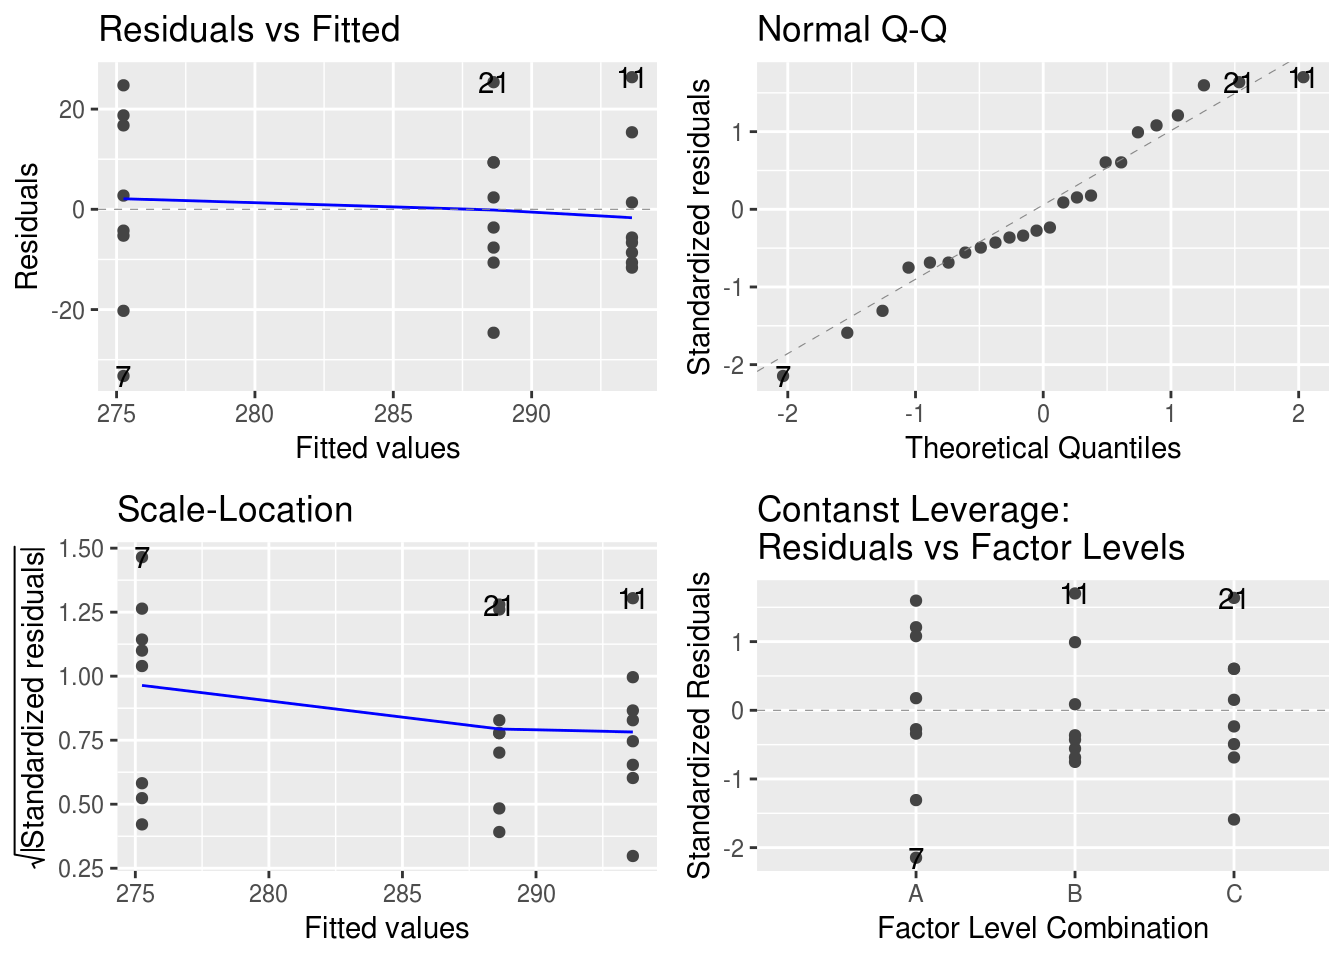
\includegraphics{anova-problemas_files/figure-latex/unnamed-chunk-2-1.pdf}

Por lo que vemos en el los gráficos no hay motivo para preocuparse por
la falta de cumplimiento de los supuestos. Pero para estar seguros
podemos usar las pruebas que vimos en la teoría: la prueba de bartlett y
la prueba de levene.

\begin{Shaded}
\begin{Highlighting}[]
\KeywordTok{bartlett.test}\NormalTok{(nitro }\OperatorTok{~}\StringTok{ }\NormalTok{trt, }\DataTypeTok{data =}\NormalTok{ nitro)}
\end{Highlighting}
\end{Shaded}

\begin{verbatim}
## 
##  Bartlett test of homogeneity of variances
## 
## data:  nitro by trt
## Bartlett's K-squared = 1.0316, df = 2, p-value = 0.597
\end{verbatim}

\begin{Shaded}
\begin{Highlighting}[]
\KeywordTok{library}\NormalTok{(car)}
\KeywordTok{leveneTest}\NormalTok{(nitro }\OperatorTok{~}\StringTok{ }\NormalTok{trt, }\DataTypeTok{data =}\NormalTok{ nitro)}
\end{Highlighting}
\end{Shaded}

\begin{verbatim}
## Warning in leveneTest.default(y = y, group = group, ...): group coerced to
## factor.
\end{verbatim}

\begin{verbatim}
## Levene's Test for Homogeneity of Variance (center = median)
##       Df F value Pr(>F)
## group  2  0.7634 0.4786
##       21
\end{verbatim}

Como ven ambas funciones trabajan de manera similar a \texttt{aov()}.
Ambas aceptan formulas y necesitan del argumento \texttt{data}.

\BeginKnitrBlock{exercise}
\protect\hypertarget{exr:unnamed-chunk-5}{}{\label{exr:unnamed-chunk-5}
}¿Qué concluirían si el test de Bartlett rechaza la hipótesis nula y el
de Levene no lo hace?
\EndKnitrBlock{exercise}

\hypertarget{recordatorio}{%
\subsection{Recordatorio}\label{recordatorio}}

Recuerden que pueden calcular las medias, desvios, etc. por grupo usando
la función \texttt{group\_by()} y a continuación la función
\texttt{summarise()}. Por ejemplo:

\begin{Shaded}
\begin{Highlighting}[]
\NormalTok{nitro }\OperatorTok\StringTok{ }
\StringTok{  }\KeywordTok{group_by}\NormalTok{(trt) }\OperatorTok\StringTok{ }
\StringTok{  }\KeywordTok{summarise}\NormalTok{(}
    \DataTypeTok{media =} \KeywordTok{mean}\NormalTok{(nitro),}
    \DataTypeTok{desvio_estandar =} \KeywordTok{sd}\NormalTok{(nitro),}
    \DataTypeTok{n =} \KeywordTok{n}\NormalTok{()}
\NormalTok{  )}
\end{Highlighting}
\end{Shaded}

\begin{verbatim}
## # A tibble: 3 x 4
##   trt   media desvio_estandar     n
##   <chr> <dbl>           <dbl> <int>
## 1 A      275.            20.0     8
## 2 B      294.            13.8     8
## 3 C      289.            15.2     8
\end{verbatim}

Con esta misma secuencia se puede calcular el test de Lilliefors para
normalidad. Aunque la secuencia algo más compleja porque el objeto que
devuelve este test no es un único número sino que son varios.

\begin{Shaded}
\begin{Highlighting}[]
\NormalTok{nitro }\OperatorTok\StringTok{ }
\StringTok{  }\KeywordTok{group_by}\NormalTok{(trt) }\OperatorTok\StringTok{ }
\StringTok{  }\KeywordTok{summarise}\NormalTok{(}\DataTypeTok{normalidad =} \KeywordTok{list}\NormalTok{(}\KeywordTok{lillie.test}\NormalTok{(nitro))) }\OperatorTok\StringTok{ }
\StringTok{  }\KeywordTok{mutate}\NormalTok{(}\DataTypeTok{statistic =} \KeywordTok{map_dbl}\NormalTok{(normalidad, }\StringTok{"statistic"}\NormalTok{),}
         \DataTypeTok{p.value =} \KeywordTok{map_dbl}\NormalTok{(normalidad, }\StringTok{"p.value"}\NormalTok{))}
\end{Highlighting}
\end{Shaded}

\begin{verbatim}
## # A tibble: 3 x 4
##   trt   normalidad  statistic p.value
##   <chr> <list>          <dbl>   <dbl>
## 1 A     <S3: htest>     0.173  0.682 
## 2 B     <S3: htest>     0.283  0.0580
## 3 C     <S3: htest>     0.144  0.897
\end{verbatim}

Voy a explicar que es lo que hice. Los pasos hasta \texttt{summarise()}
son similares a los que se usan para calcular la media, desvío estándar,
etc. La función \texttt{lillie.test} devuelve varios números distintos y
¡\texttt{summarise} quiere solo un número! Para resolver este
incoveniente hay que envolver todos estos números en otra objeto.
Imaginen que cada número está dentro de una caja, si metemos todos estas
cajas dentro de un cajón entonces tenemos solo un cajón por cada uno de
nuestros niveles. Al cajón de está analogía se lo conoce como lista en R
(\texttt{list}) y puede contener cajas de de cualquier tipo ¡Incluso
mezcladas!. Ahora, la lista es cómoda para trabajar como estructura
intermedia en nuestros calculos, pero no es cómoda para ver los
resultados. De cada uno esos cajones queremos extraer la caja con los
números que nos interesan, el valor del estadístico y la probabilidad
(\(P(X>x)\)). Para eso use la función \texttt{mutate} que agrega o
cambia el valor de una columna y la función \texttt{map}. Es un poco
compleja de explicar ahora como funciona esta última función, pero por
ahora solo necesitan saber que la estamos usando para extraer la cajas
de los cajones. Entonces, para ponerlo en castellano lo que estoy
haciendo se puede traducir como: con los datos de \texttt{nitro}
agrupalos por la variable \texttt{trt}; luego resumilos en una nueva
variable \texttt{normalidad}, que es el resultado de probar la
normalidad con la función \texttt{lillie.test()} de la variable
\texttt{nitro}; luego, a ese resultado, agregar la variable
\texttt{statistic} que es igual a extraer la caja \texttt{statistic} del
cajón \texttt{normalidad} y la variable \texttt{p.value} que es igual a
extraer la caja \texttt{p.value} del cajón \texttt{normalidad}.

\BeginKnitrBlock{exercise}
\protect\hypertarget{exr:unnamed-chunk-8}{}{\label{exr:unnamed-chunk-8} }1.
¿Cuales son las hipótesis que se prueban en la prueba de Lilliefors?

\begin{enumerate}
\def\labelenumi{\arabic{enumi}.}
\setcounter{enumi}{1}
\tightlist
\item
  ¿Se rechaza alguna de ellas?
\end{enumerate}
\EndKnitrBlock{exercise}

\hypertarget{problemas}{%
\section{Problemas}\label{problemas}}

Primero bajen la planilla para completar los problemas:

\begin{Shaded}
\begin{Highlighting}[]
\KeywordTok{download.file}\NormalTok{(}\StringTok{"git.io/informe-anova.Rmd"}\NormalTok{, }\StringTok{"informe-anova.Rmd"}\NormalTok{)}
\end{Highlighting}
\end{Shaded}

\begin{enumerate}
\def\labelenumi{\arabic{enumi}.}
\tightlist
\item
  Se lleva a cabo una experiencia para poner a prueba el efecto de 6
  fertilizantes sobre el crecimiento de la soja, obteniéndose la
  siguiente tabla de ANOVA:
\end{enumerate}

\begin{longtable}[]{@{}ccccc@{}}
\toprule
\begin{minipage}[b]{0.23\columnwidth}\centering
Fte.de.Variación\strut
\end{minipage} & \begin{minipage}[b]{0.12\columnwidth}\centering
SC\strut
\end{minipage} & \begin{minipage}[b]{0.06\columnwidth}\centering
GL\strut
\end{minipage} & \begin{minipage}[b]{0.08\columnwidth}\centering
F\strut
\end{minipage} & \begin{minipage}[b]{0.10\columnwidth}\centering
p\strut
\end{minipage}\tabularnewline
\midrule
\endhead
\begin{minipage}[t]{0.23\columnwidth}\centering
Entre\strut
\end{minipage} & \begin{minipage}[t]{0.12\columnwidth}\centering
754.25\strut
\end{minipage} & \begin{minipage}[t]{0.06\columnwidth}\centering
5\strut
\end{minipage} & \begin{minipage}[t]{0.08\columnwidth}\centering
2.23\strut
\end{minipage} & \begin{minipage}[t]{0.10\columnwidth}\centering
0.0644\strut
\end{minipage}\tabularnewline
\begin{minipage}[t]{0.23\columnwidth}\centering
Dentro\strut
\end{minipage} & \begin{minipage}[t]{0.12\columnwidth}\centering
3646.08\strut
\end{minipage} & \begin{minipage}[t]{0.06\columnwidth}\centering
54\strut
\end{minipage} & \begin{minipage}[t]{0.08\columnwidth}\centering
\strut
\end{minipage} & \begin{minipage}[t]{0.10\columnwidth}\centering
\strut
\end{minipage}\tabularnewline
\bottomrule
\end{longtable}

\begin{itemize}
\tightlist
\item
  Calcular la potencia. Enuncie sus conclusiones.
\item
  ¿Cual es el n necesario para tener una potencia de 90\%?
\end{itemize}

Para calcular la potencia en R se puede usar la función
\texttt{power.anova.test()} del paquete \texttt{pwr}. Esta función puede
calcular tanto la potencia de una prueba como el n necesario para
alcanzar cierta potencia, dependiendo de que dato falte completar. Para
eso necesita:

\begin{itemize}
\tightlist
\item
  El número de grupos
\item
  El n de cada grupo (esto implica que solo da resultados aproximados
  con datos desbalanceados)
\item
  la varianza entre grupos.
\item
  la varianza dentro de los grupos.
\end{itemize}

A partir de la tabla de ANOVA es posible derivar todos los datos.

\begin{Shaded}
\begin{Highlighting}[]
\CommentTok{# Número de grupos. Recordar que GL entre = K - 1 }
\NormalTok{g <-}\StringTok{ }\DecValTok{5} \OperatorTok{+}\StringTok{ }\DecValTok{1}
\CommentTok{# Número de réplicas por grupo N-I/I}
\NormalTok{n <-}\StringTok{ }\NormalTok{(}\DecValTok{54} \OperatorTok{+}\StringTok{ }\NormalTok{g) }\OperatorTok{/}\StringTok{ }\NormalTok{g}

\CommentTok{# bv <- (as.numeric(as.character(soja$SC[1])) +}
\CommentTok{#          as.numeric(as.character(soja$SC[2]))) / (n*g-1)/n}

\CommentTok{# Varianza entre grupo CM entre /n}
\NormalTok{bv <-}\StringTok{ }\FloatTok{754.25} \OperatorTok{/}\StringTok{ }\DecValTok{5} \OperatorTok{/}\StringTok{ }\NormalTok{n}

\CommentTok{# Varianza dentro de grupos CM dentro}
\NormalTok{wv <-}\StringTok{ }\FloatTok{3648.08}\OperatorTok{/}\StringTok{ }\DecValTok{54}



\KeywordTok{power.anova.test}\NormalTok{(}\DataTypeTok{groups =}\NormalTok{ g, }\DataTypeTok{n =}\NormalTok{ n, }\DataTypeTok{between.var =}\NormalTok{ bv, }\DataTypeTok{within.var =}\NormalTok{ wv)}
\end{Highlighting}
\end{Shaded}

\begin{verbatim}
## 
##      Balanced one-way analysis of variance power calculation 
## 
##          groups = 6
##               n = 10
##     between.var = 15.085
##      within.var = 67.55704
##       sig.level = 0.05
##           power = 0.6821423
## 
## NOTE: n is number in each group
\end{verbatim}

\begin{enumerate}
\def\labelenumi{\arabic{enumi}.}
\setcounter{enumi}{1}
\tightlist
\item
  Fueron ensayados dos cebos distintos para estimar si existía una
  diferencia significativa en función de su consumo por ratones
  silvestres. Los datos de la tabla se obtuvieron en cinco sitios
  diferentes por cebo y están expresados como porcentaje de consumo:
\end{enumerate}

\begin{Shaded}
\begin{Highlighting}[]
\NormalTok{cebos}
\end{Highlighting}
\end{Shaded}

\begin{verbatim}
##    A  B
## 1 10 15
## 2 15 20
## 3 12 16
## 4 20 25
## 5 14 20
\end{verbatim}

\begin{itemize}
\tightlist
\item
  Analizar la significación de estas observaciones.
\item
  ¿Qué transformación es conveniente utlizar teniendo en cuenta el tipo
  de dato?
\item
  La potencia de la prueba.
\end{itemize}

\begin{enumerate}
\def\labelenumi{\arabic{enumi}.}
\setcounter{enumi}{2}
\tightlist
\item
  Durante el estudio del control del fotoperíodo de la reproducción del
  alga roja Porphira, se llevó a cabo un experimento para examinar el
  efecto de la interrupción de largos períodos de oscuridad, mediante un
  período de iluminación de 30 minutos con luz de diferentes longitudes
  de onda, y se contaron los esporangios en un volumen fijo de material.
  Se obtuvieron 4 réplicas para cada una de las cinco longitudes de
  onda.
\end{enumerate}

\begin{verbatim}
##        Color N\xfamero.de.esporangios  NA. NA..1 NA..2
## 1       Azul                     7720 7490  7986  7382
## 2      Verde                     7918 7948  7632  8215
## 3   Amarillo                     6495 7101  7412  7006
## 4       Rojo                     4741 4150  5315  4810
## 5 Infrarrojo                     7520 7418  7937  7118
\end{verbatim}

Teóricamente solamente la luz roja tiene efecto sobre el número de
esporangios.

\begin{enumerate}
\def\labelenumi{\alph{enumi})}
\tightlist
\item
  Realizar un análisis para decidir si hay diferencia entre los efectos
  de las longitudes de onda.
\item
  Poner a prueba el supuesto teórico.
\item
  ¿Puede inferirse algún otro resultado?
\end{enumerate}

\hypertarget{contrastes}{%
\subsection{Contrastes}\label{contrastes}}

En R existen varias formas de hacer contrastes. Una de las más prácticas
es usar el paquete \texttt{emmeans} que además de estimar la medias
marginales también permite realizar comparaciones de a pares. La función
\texttt{eemeans} devuelve por defecto las medias marginales junto con
los errores estándar, grados de libertad, e intervalos de confianza.

\begin{Shaded}
\begin{Highlighting}[]
\NormalTok{alga.em <-}\StringTok{ }\KeywordTok{emmeans}\NormalTok{(alga.aov, }\OperatorTok{~}\StringTok{ }\NormalTok{Color)}
\NormalTok{alga.em}
\end{Highlighting}
\end{Shaded}

\begin{verbatim}
##  Color       emmean       SE df lower.CL upper.CL
##  Amarillo   7003.50 175.4702 15 6629.494 7377.506
##  Azul       7644.50 175.4702 15 7270.494 8018.506
##  Infrarrojo 7498.25 175.4702 15 7124.244 7872.256
##  Rojo       4754.00 175.4702 15 4379.994 5128.006
##  Verde      7928.25 175.4702 15 7554.244 8302.256
## 
## Confidence level used: 0.95
\end{verbatim}

También puede ser usada para estimar la comparación de a pares. Por
defecto, usa el método de Tukey. Se pueden usar otros métodos como
Bonferroni (\texttt{bonferroni}), Scheffé (\texttt{scheffe}), LSD
(\texttt{none}), y otro más (para más detalles ver
\texttt{?summary.emmGrid} sección \emph{P-value adjustment})

\begin{Shaded}
\begin{Highlighting}[]
\KeywordTok{pairs}\NormalTok{(alga.em, }\DataTypeTok{adjust =} \StringTok{"none"}\NormalTok{)}
\end{Highlighting}
\end{Shaded}

\begin{verbatim}
##  contrast              estimate       SE df t.ratio p.value
##  Amarillo - Azul        -641.00 248.1523 15  -2.583  0.0208
##  Amarillo - Infrarrojo  -494.75 248.1523 15  -1.994  0.0647
##  Amarillo - Rojo        2249.50 248.1523 15   9.065  <.0001
##  Amarillo - Verde       -924.75 248.1523 15  -3.727  0.0020
##  Azul - Infrarrojo       146.25 248.1523 15   0.589  0.5644
##  Azul - Rojo            2890.50 248.1523 15  11.648  <.0001
##  Azul - Verde           -283.75 248.1523 15  -1.143  0.2708
##  Infrarrojo - Rojo      2744.25 248.1523 15  11.059  <.0001
##  Infrarrojo - Verde     -430.00 248.1523 15  -1.733  0.1036
##  Rojo - Verde          -3174.25 248.1523 15 -12.792  <.0001
\end{verbatim}

\begin{Shaded}
\begin{Highlighting}[]
\KeywordTok{LSD.test}\NormalTok{(alga.aov, }\StringTok{"Color"}\NormalTok{, }\DataTypeTok{console =} \OtherTok{TRUE}\NormalTok{)}
\end{Highlighting}
\end{Shaded}

\begin{verbatim}
## 
## Study: alga.aov ~ "Color"
## 
## LSD t Test for esporangios 
## 
## Mean Square Error:  123159.2 
## 
## Color,  means and individual ( 95 %) CI
## 
##            esporangios      std r      LCL      UCL  Min  Max
## Amarillo       7003.50 380.7698 4 6629.494 7377.506 6495 7412
## Azul           7644.50 267.7679 4 7270.494 8018.506 7382 7986
## Infrarrojo     7498.25 338.6270 4 7124.244 7872.256 7118 7937
## Rojo           4754.00 477.0891 4 4379.994 5128.006 4150 5315
## Verde          7928.25 238.3868 4 7554.244 8302.256 7632 8215
## 
## Alpha: 0.05 ; DF Error: 15
## Critical Value of t: 2.13145 
## 
## least Significant Difference: 528.9242 
## 
## Treatments with the same letter are not significantly different.
## 
##            esporangios groups
## Verde          7928.25      a
## Azul           7644.50      a
## Infrarrojo     7498.25     ab
## Amarillo       7003.50      b
## Rojo           4754.00      c
\end{verbatim}

También se pueden graficar los intervalos de confianza de las medias
estimadas, y de las comparaciones de entre ellas.

\begin{Shaded}
\begin{Highlighting}[]
\KeywordTok{plot}\NormalTok{(alga.em, }\DataTypeTok{comparisons =} \OtherTok{TRUE}\NormalTok{)}
\end{Highlighting}
\end{Shaded}

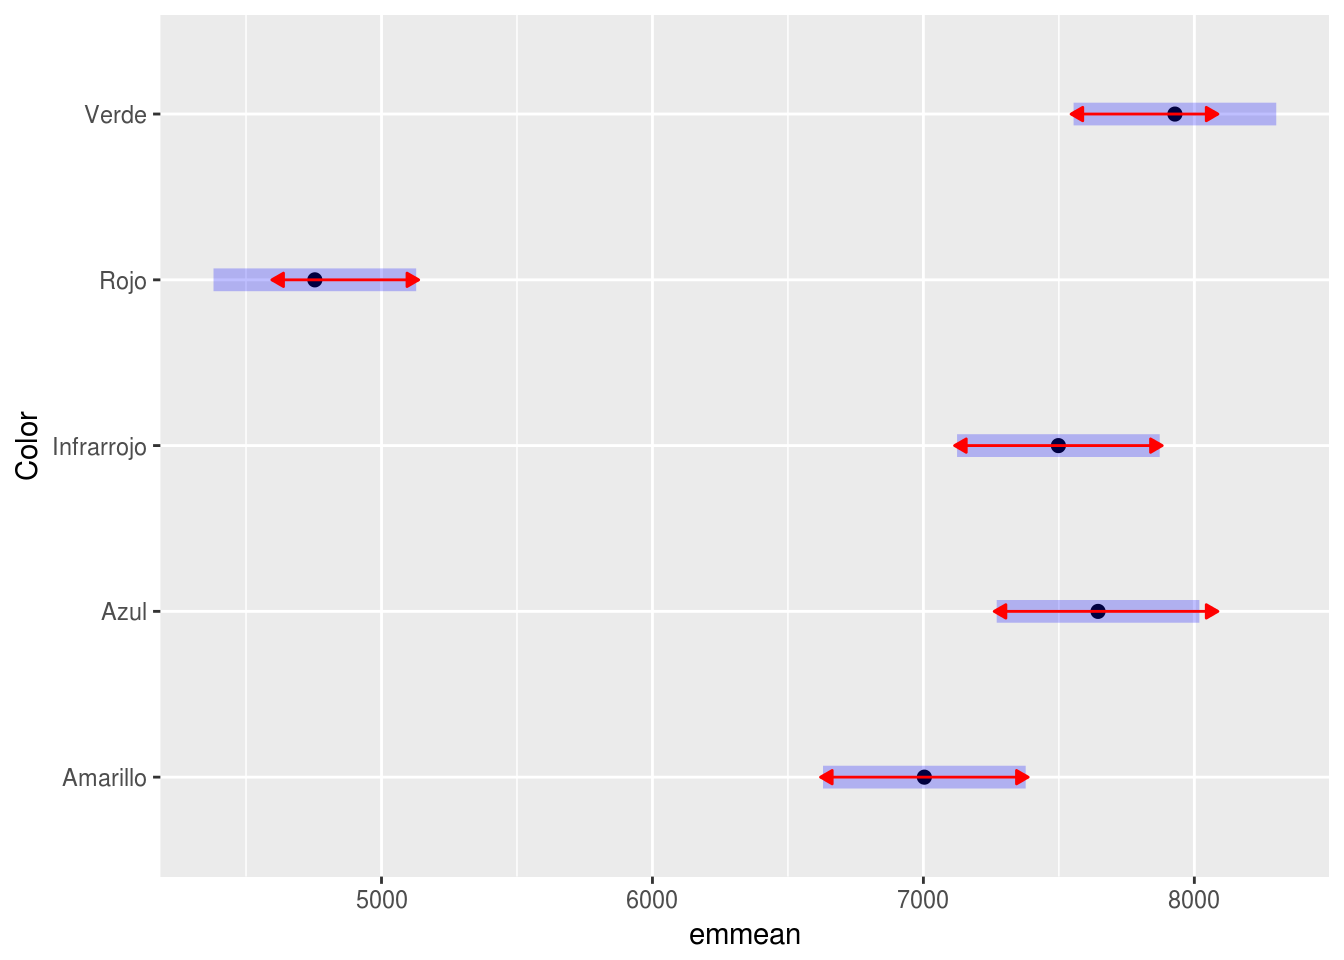
\includegraphics{anova-problemas_files/figure-latex/unnamed-chunk-14-1.pdf}

Las barras azules son los intervalos de confianza para las medias y las
flechas rojas son los intervalos de confianza de las comparaciones entre
ellos. Si las flechas no se superponen las diferencias son
significativas entre ellos.

También es posible obtener lo que se llama \emph{compact letter display}
que es una forma muy práctica de ver comparaciones.

\begin{Shaded}
\begin{Highlighting}[]
\KeywordTok{cld}\NormalTok{(alga.em)}
\end{Highlighting}
\end{Shaded}

\begin{verbatim}
##        Color  emmean       SE df lower.CL upper.CL .group
## 4       Rojo 4754.00 175.4702 15 4379.994 5128.006    1  
## 1   Amarillo 7003.50 175.4702 15 6629.494 7377.506     2 
## 3 Infrarrojo 7498.25 175.4702 15 7124.244 7872.256     23
## 2       Azul 7644.50 175.4702 15 7270.494 8018.506     23
## 5      Verde 7928.25 175.4702 15 7554.244 8302.256      3
\end{verbatim}

Los niveles que no comparten números o letras son significativamente
distintos.

También podemos ver cuales son los coeficientes de los contrastes
usados.

\begin{Shaded}
\begin{Highlighting}[]
\KeywordTok{coef}\NormalTok{(}\KeywordTok{pairs}\NormalTok{(alga.em))}
\end{Highlighting}
\end{Shaded}

\begin{verbatim}
##                 Color c.1 c.2 c.3 c.4 c.5 c.6 c.7 c.8 c.9 c.10
## Amarillo     Amarillo   1   1   1   1   0   0   0   0   0    0
## Azul             Azul  -1   0   0   0   1   1   1   0   0    0
## Infrarrojo Infrarrojo   0  -1   0   0  -1   0   0   1   1    0
## Rojo             Rojo   0   0  -1   0   0  -1   0  -1   0    1
## Verde           Verde   0   0   0  -1   0   0  -1   0  -1   -1
\end{verbatim}

Ahora, la pregunta que nos hacen es poner a prueba el supuesto teórico
de que solo las roja es efectiva. Podemos hacerlo de dos formas
distintas. Una por contrastes ortogonales. Es quizás el método más
complicado, aunque más poderoso, de hacer. Primero debemos implementar
nuestros coeficientes. Los niveles del factor son ordenados por orden
alfabético a menos que indiquemos otro orden. Por lo tanto, el orden de
los niveles de \texttt{Color} es: Amarillo, Azul, Infrarrojo, Rojo,
Creamos una matriz de tamaño I x (I-1). Cada columna es un contraste.

\begin{Shaded}
\begin{Highlighting}[]
\NormalTok{contraste.algas <-}\StringTok{ }\KeywordTok{matrix}\NormalTok{(}\KeywordTok{c}\NormalTok{(}\OperatorTok{-}\DecValTok{1}\NormalTok{, }\DecValTok{-1}\NormalTok{, }\DecValTok{-1}\NormalTok{ , }\DecValTok{4}\NormalTok{, }\DecValTok{-1}\NormalTok{,}
                            \DecValTok{-1}\NormalTok{, }\DecValTok{-1}\NormalTok{, }\DecValTok{-1}\NormalTok{, }\DecValTok{0}\NormalTok{, }\DecValTok{3}\NormalTok{,}
                            \DecValTok{-1}\NormalTok{, }\DecValTok{-1}\NormalTok{, }\DecValTok{2}\NormalTok{, }\DecValTok{0}\NormalTok{ , }\DecValTok{0}\NormalTok{,}
                            \DecValTok{1}\NormalTok{, }\DecValTok{-1}\NormalTok{, }\DecValTok{0}\NormalTok{, }\DecValTok{0}\NormalTok{, }\DecValTok{0}\NormalTok{),}
                          \DataTypeTok{nrow =} \DecValTok{5}\NormalTok{)}
\KeywordTok{row.names}\NormalTok{(contraste.algas) <-}\StringTok{ }\KeywordTok{levels}\NormalTok{(alga}\OperatorTok{$}\NormalTok{Color)}
\KeywordTok{colnames}\NormalTok{(contraste.algas) <-}\StringTok{ }\KeywordTok{paste}\NormalTok{(}\StringTok{"c"}\NormalTok{, }\DecValTok{1}\OperatorTok{:}\DecValTok{4}\NormalTok{, }\DataTypeTok{sep =} \StringTok{"."}\NormalTok{)}
\NormalTok{contraste.algas}
\end{Highlighting}
\end{Shaded}

\begin{verbatim}
##            c.1 c.2 c.3 c.4
## Amarillo    -1  -1  -1   1
## Azul        -1  -1  -1  -1
## Infrarrojo  -1  -1   2   0
## Rojo         4   0   0   0
## Verde       -1   3   0   0
\end{verbatim}

\begin{Shaded}
\begin{Highlighting}[]
\CommentTok{# Comprobar que son ortogonales, fuera de la diagonal debe dar 0}
\KeywordTok{crossprod}\NormalTok{(contraste.algas)}
\end{Highlighting}
\end{Shaded}

\begin{verbatim}
##     c.1 c.2 c.3 c.4
## c.1  20   0   0   0
## c.2   0  12   0   0
## c.3   0   0   6   0
## c.4   0   0   0   2
\end{verbatim}

Una vez hecho la matriz de coeficientes, la usamos dentro de la función
\texttt{aov} especificando el argumento \texttt{contrasts} que debe ser
una lista con nombres igual a los variables explicatorias.

\begin{Shaded}
\begin{Highlighting}[]
\NormalTok{alga.aov_or <-}\StringTok{ }\KeywordTok{aov}\NormalTok{(esporangios }\OperatorTok{~}\StringTok{ }\NormalTok{Color, }\DataTypeTok{data =}\NormalTok{ alga, }
                      \DataTypeTok{contrasts =} \KeywordTok{list}\NormalTok{(}\DataTypeTok{Color =}\NormalTok{ contraste.algas))}
\end{Highlighting}
\end{Shaded}

Luego hay que hacer algo similar para que \texttt{summary} muestre esos
contrastes. Especificar el argumento \texttt{split} que también tiene
que ser una lista con los nombres de los variables explicatorias, pero
dentro de cada uno hay un vector con nombres donde el número indica que
contraste es.

\begin{Shaded}
\begin{Highlighting}[]
\KeywordTok{summary}\NormalTok{(alga.aov_or, }\DataTypeTok{split =} \KeywordTok{list}\NormalTok{(}\DataTypeTok{Color =} \KeywordTok{c}\NormalTok{(}\StringTok{"Rojo vs Todos"}\NormalTok{ =}\StringTok{ }\DecValTok{1}\NormalTok{,}
                                            \StringTok{"Verde vs Amarillo, Azul, Infrarrojo"}\NormalTok{  =}\StringTok{ }\DecValTok{2}\NormalTok{,}
                                            \StringTok{"Amarillo Azul vs Infrarrojo"}\NormalTok{ =}\StringTok{ }\DecValTok{3}\NormalTok{,}
                                            \StringTok{"Amarillo vs Azul"}\NormalTok{ =}\StringTok{ }\DecValTok{4}\NormalTok{)))}
\end{Highlighting}
\end{Shaded}

\begin{verbatim}
##                                              Df   Sum Sq  Mean Sq F value
## Color                                         4 26255709  6563927  53.296
##   Color: Rojo vs Todos                        1 24458084 24458084 198.589
##   Color: Verde vs Amarillo, Azul, Infrarrojo  1   894894   894894   7.266
##   Color: Amarillo Azul vs Infrarrojo          1    80968    80968   0.657
##   Color: Amarillo vs Azul                     1   821762   821762   6.672
## Residuals                                    15  1847388   123159        
##                                                Pr(>F)    
## Color                                        1.09e-08 ***
##   Color: Rojo vs Todos                       4.67e-10 ***
##   Color: Verde vs Amarillo, Azul, Infrarrojo   0.0166 *  
##   Color: Amarillo Azul vs Infrarrojo           0.4301    
##   Color: Amarillo vs Azul                      0.0208 *  
## Residuals                                                
## ---
## Signif. codes:  0 '***' 0.001 '**' 0.01 '*' 0.05 '.' 0.1 ' ' 1
\end{verbatim}

Noten las diferencias de resultados entres las comparaciones múltiples.

La otra forma es usar comparaciones de a pares pero solo usando
tratamientos vs control. En este caso nuestro ``control'' es el color
rojo. Se puede hacer usando \texttt{emmeans} y resulta mucho más
sencillo. La función a usar es \texttt{contrast}. Además de indicar el
objeto sobre el que hay que realizar los contrastes, también es
necesario indicar el método (\texttt{method}), y opcionalmente el número
de nivel que corresponde al tratamiento control (\texttt{ref})

\begin{Shaded}
\begin{Highlighting}[]
\KeywordTok{contrast}\NormalTok{(}\DataTypeTok{object =}\NormalTok{ alga.em, }\DataTypeTok{method =} \StringTok{"trt.vs.ctrl"}\NormalTok{, }\DataTypeTok{ref =} \DecValTok{4}\NormalTok{)}
\end{Highlighting}
\end{Shaded}

\begin{verbatim}
##  contrast          estimate       SE df t.ratio p.value
##  Amarillo - Rojo    2249.50 248.1523 15   9.065  <.0001
##  Azul - Rojo        2890.50 248.1523 15  11.648  <.0001
##  Infrarrojo - Rojo  2744.25 248.1523 15  11.059  <.0001
##  Verde - Rojo       3174.25 248.1523 15  12.792  <.0001
## 
## P value adjustment: dunnettx method for 4 tests
\end{verbatim}

\begin{enumerate}
\def\labelenumi{\arabic{enumi}.}
\setcounter{enumi}{3}
\item
  La faciolasis es una enfermedad parasitaria producida por la
  \emph{Fasciola hepatica} (trematode hepático). Los trematodes adultos
  viven en el conducto biliar del huésped, donde segregan cantidades
  significativas de ciertos aminoácidos, en especial prolina; el huésped
  presenta, como característica, anemia (reducción en los glóbulos rojos
  de la sangre). Se tomaron 40 ratas Wistar, sanas de aproximadamente
  igual peso y edad, se dividieron al azar en 4 grupos de 10 ratas cada
  uno. Se adaptó un aparato para infundir material directamente al
  conducto biliar de las ratas mediante una cánula. Las ratas del grupo
  I recibieron 20 minimoles de prolina disuelta en suero fisiológico,
  las del grupo II recibieron un cóctel consistente siete aminoácidos
  (excluyendo prolina) segregados por el trematode, también disuelto en
  suero fisiológico; el grupo III recibió lo mismo que el II más el
  agregado de 20 milimoles de prolina (simulando a lo segregado por el
  trematode) y el grupo IV sólo se trató con suero fisiológico. En todos
  los casos se tomó como variable el número de glóbulos rojos del
  huésped, expresados en millones por mm3 de sangre. Los resultados se
  presentan en la siguiente tabla:

\begin{verbatim}
    GRUPO.I            GRUPO.II           GRUPO.III
\end{verbatim}

  1 20 mmol prolina mezcla aa - prolina mezcla aa + prolina 2 6.07 5.69
  5.61 3 5.02 5.54 5.40 4 5.69 5.35 5.26 5 5.43 5.11 4.99 6 5.87 5.94
  5.44 7 5.55 5.25 5.13 8 5.64 6.02 5.21 9 5.95 5.64 5.52 10 5.20 5.11
  4.79 11 5.40 5.04 4.92 GRUPO.IV 1 suero fisiológico 2 7.35 3 7.11 4
  6.99 5 6.72 6 7.16 7 6.85 8 6.94 9 7.25 10 6.51 11 6.65
\end{enumerate}

\begin{enumerate}
\def\labelenumi{\alph{enumi})}
\tightlist
\item
  Plantear y comprobar todos los supuestos para la validez de las
  pruebas estadísticas utilizadas.
\item
  ¿Está asociada la reducción del número de glóbulos rojos de la sangre
  del huésped con la segregación de aminoácidos por el trematode?
\item
  ¿Está específicamente asociado a la segregación de prolina?
\item
  Realice un breve comentario sobre el diseño del experimento.
\end{enumerate}

\begin{enumerate}
\def\labelenumi{\arabic{enumi}.}
\setcounter{enumi}{4}
\tightlist
\item
  Se realiza una experiencia a fin de comparar tres métodos diferentes
  para determinar el contenido de oxígeno disuelto en el agua de lagos.
  Se extrae una muestra aleatoria de 18 muestras de agua de un lago, las
  cuales se dividen al azar en tres grupos de igual tamaño y cada uno de
  los grupos es asignado al azar a uno de los métodos que se quiere
  comparar. Se obtienen los siguientes resultados, expresados en
  mg/litro:
\end{enumerate}

Método.1 Método.2 Método.3 1 832 1023 8710 2 324 832 1660 3 550 1318
5495 4 617 1995 3981 5 525 832 2138 6 1349 912 3548 7 501 646 5130

\begin{enumerate}
\def\labelenumi{\alph{enumi})}
\tightlist
\item
  Comprobar las suposiciones del ANOVA
\item
  Poner a prueba la hipótesis ``No hay efecto del método en la
  determinación de oxígeno en el agua del lago''. Indicar P.
\item
  Realizar comparaciones entre métodos, utilizando todos los métodos de
  contraste conocidos e indicar cuáles serían los adecuados a este
  problema particular.
\item
  Hallar la potencia de la prueba para alguna hipótesis alternativa.
\item
  Estimar el tamaño de la muestra (¿de qué?) con la que debería trabajar
  para tener una potencia del 95\%, con una probabilidad de cometer
  error de Tipo I del 5\%.
\end{enumerate}

\begin{enumerate}
\def\labelenumi{\arabic{enumi}.}
\setcounter{enumi}{5}
\tightlist
\item
  En un estudio sobre viabilidad, se aíslan tres parejas de
  \emph{Drosophila melanogaster} en 10 frascos y se hace un recuento del
  número de huevos al cabo de 8 días. Esta experiencia se repite 4 veces
  con parejas distintas. Los resultados obtenidos son:
\end{enumerate}

\begin{Shaded}
\begin{Highlighting}[]
\NormalTok{mosca}
\end{Highlighting}
\end{Shaded}

\begin{verbatim}
##    Serie.1 Serie.2 Serie.3 Serie.4
## 1       47      28      32      50
## 2       36      31      41      44
## 3       22      32      44      67
## 4       69      45      17      63
## 5       68      72      96      87
## 6       57     101      20      74
## 7       37      55      45      21
## 8      108      27      55      54
## 9       29      49      36      91
## 10      72      36      72      72
\end{verbatim}

\begin{enumerate}
\def\labelenumi{\alph{enumi}.}
\tightlist
\item
  ¿Es posible reunir las cuatro series en una sola para efectuar un
  análisis conjunto de la viabilidad? Trabajar con = 0.05
\item
  Hallar la potencia de la prueba realizada cuando se dan ciertas
  alternativas.
\item
  Estimar el tamaño de la muestra con que debería trabajar en cada
  tratamiento para tener una potencia mayor del 95\%.
\end{enumerate}

\hypertarget{anova-de-dos-factores}{%
\chapter{ANOVA DE DOS FACTORES}\label{anova-de-dos-factores}}

\hypertarget{ventajas-de-los-estudios-multifactoriales}{%
\section{Ventajas de los estudios
multifactoriales}\label{ventajas-de-los-estudios-multifactoriales}}

\hypertarget{eficiencia}{%
\subsection{Eficiencia:}\label{eficiencia}}

\hypertarget{cantidad-de-informacion-permiten-estudiar-la-interaccion-de-los-factores.}{%
\subsubsection{\texorpdfstring{Cantidad de Información: Permiten
estudiar la \emph{interacción} de los
factores.}{Cantidad de Información: Permiten estudiar la interacción de los factores.}}\label{cantidad-de-informacion-permiten-estudiar-la-interaccion-de-los-factores.}}

\emph{Validez de las decisiones}: los experimentos multifactoriales
también pueden robustecer la validez de las decisiones.

\emph{Comentarios}:

\begin{enumerate}
\def\labelenumi{\arabic{enumi}.}
\item
  Los análisis multifactoriales permiten una evaluación efectiva de los
  efectos de la interacción y economiza el número de casos requeridos
  para el análisis.
\item
  Experimentos involucrando muchos factores, cada uno con numerosos
  niveles, se vuelven complejos, costosos e insumen tiempo.
\end{enumerate}

\hypertarget{elementos-del-modelo}{%
\section{Elementos del Modelo}\label{elementos-del-modelo}}

\emph{Ejemplo}: Consideremos un estudio de dos factores, en el cual son
de interés los efectos del sexo y la edad en el aprendizaje de una
tarea. El factor edad lo definimos en términos de sólo tres niveles
(adolescente, adulto joven, anciano).

La respuesta para un dado tratamiento, en un estudio de dos factores, es
indicada por µij, donde i hace referencia al nivel del factor \(A\)
(\(i = 1,2,\ldots,I\)) y j se refiere al nivel del factor \(B\)
(\(j = 1,2,\ldots,J\)).

\begin{longtable}[]{@{}lllll@{}}
\caption{\label{tab:aprendizaje1} Tiempo de aprendizaje (en minutos) en
mujeres de y hombres de tres edades. Caso sin interacción y sin efecto
del factor \emph{Sexo}.}\tabularnewline
\toprule
\begin{minipage}[b]{0.15\columnwidth}\raggedright
SEXO\strut
\end{minipage} & \begin{minipage}[b]{0.26\columnwidth}\raggedright
EDAD\strut
\end{minipage} & \begin{minipage}[b]{0.15\columnwidth}\raggedright
\strut
\end{minipage} & \begin{minipage}[b]{0.12\columnwidth}\raggedright
\strut
\end{minipage} & \begin{minipage}[b]{0.17\columnwidth}\raggedright
\strut
\end{minipage}\tabularnewline
\midrule
\endfirsthead
\toprule
\begin{minipage}[b]{0.15\columnwidth}\raggedright
SEXO\strut
\end{minipage} & \begin{minipage}[b]{0.26\columnwidth}\raggedright
EDAD\strut
\end{minipage} & \begin{minipage}[b]{0.15\columnwidth}\raggedright
\strut
\end{minipage} & \begin{minipage}[b]{0.12\columnwidth}\raggedright
\strut
\end{minipage} & \begin{minipage}[b]{0.17\columnwidth}\raggedright
\strut
\end{minipage}\tabularnewline
\midrule
\endhead
\begin{minipage}[t]{0.15\columnwidth}\raggedright
\strut
\end{minipage} & \begin{minipage}[t]{0.26\columnwidth}\raggedright
\textbf{Adolescente (j=1)}\strut
\end{minipage} & \begin{minipage}[t]{0.15\columnwidth}\raggedright
\textbf{Adulto joven (j=2)}\strut
\end{minipage} & \begin{minipage}[t]{0.12\columnwidth}\raggedright
\textbf{Anciano (j=3) }\strut
\end{minipage} & \begin{minipage}[t]{0.17\columnwidth}\raggedright
\(\mathbf{\mu_{i\bullet}}\)\strut
\end{minipage}\tabularnewline
\begin{minipage}[t]{0.15\columnwidth}\raggedright
\textbf{Masculino (\(i = 1\))}\strut
\end{minipage} & \begin{minipage}[t]{0.26\columnwidth}\raggedright
9 (\(\mu_{11}\))\strut
\end{minipage} & \begin{minipage}[t]{0.15\columnwidth}\raggedright
11 (\(\mu_{12}\))\strut
\end{minipage} & \begin{minipage}[t]{0.12\columnwidth}\raggedright
16 (\(\mu_{13}\))\strut
\end{minipage} & \begin{minipage}[t]{0.17\columnwidth}\raggedright
12 (\(\mu_{1\bullet}\))\strut
\end{minipage}\tabularnewline
\begin{minipage}[t]{0.15\columnwidth}\raggedright
\textbf{Femenino (\(i = 2\))}\strut
\end{minipage} & \begin{minipage}[t]{0.26\columnwidth}\raggedright
9 (\(\mu_{21}\))\strut
\end{minipage} & \begin{minipage}[t]{0.15\columnwidth}\raggedright
11 (\(\mu_{22}\))\strut
\end{minipage} & \begin{minipage}[t]{0.12\columnwidth}\raggedright
16 (\(\mu_{23}\))\strut
\end{minipage} & \begin{minipage}[t]{0.17\columnwidth}\raggedright
12 (\(\mu_{2\bullet}\))\strut
\end{minipage}\tabularnewline
\begin{minipage}[t]{0.15\columnwidth}\raggedright
\textbf{\(\mu_{\bullet j}\)}\strut
\end{minipage} & \begin{minipage}[t]{0.26\columnwidth}\raggedright
9 (\(\mu_{\bullet1}\))\strut
\end{minipage} & \begin{minipage}[t]{0.15\columnwidth}\raggedright
11 (\(\mu_{\bullet2}\))\strut
\end{minipage} & \begin{minipage}[t]{0.12\columnwidth}\raggedright
16 (\(\mu_{\bullet3}\))\strut
\end{minipage} & \begin{minipage}[t]{0.17\columnwidth}\raggedright
12 (\(\mu_{\bullet\bullet}\))\strut
\end{minipage}\tabularnewline
\bottomrule
\end{longtable}

Indicamos

\[
\mu_{\bullet j} = \frac{\sum_{i = 1}^{I}\mu_{ij}}{I}
\]

y

\[
\mu_{i \bullet} = \frac{\sum_{j = 1}^{J}\mu_{ij}}{J}
\]

La media general se indica cómo \(\mu_{\bullet \bullet}\), y es definida
en las siguientes formas equivalentes:

\[
\begin{aligned}
\mu_{\bullet \bullet} &= \frac{\sum_{i = 1}^{I}{\sum_{j = 1}^{J}\mu_{ij}}}{ij}\\
\mu_{\bullet \bullet} &= \frac{\sum_{i = 1}^{I}\mu_{i \bullet}}{I}\\
\mu_{\bullet \bullet} &= \frac{\sum_{j = 1}^{J}\mu_{\bullet j}}{J}
\end{aligned}
\]

\hypertarget{efectos-principales}{%
\subsection{Efectos principales}\label{efectos-principales}}

Definimos el efecto principal del factor \(A\) al i-ésimo nivel, como:

\[
\alpha_{i} = \mu_{i \bullet} - \mu_{\bullet \bullet}
\]

En el ejemplo:

\[
\alpha_{1} = \mu_{1 \bullet} - \mu_{\bullet \bullet} = 912 = - 3
\]

De forma similar, el efecto principal del j-ésimo nivel del facto B se
define:

\[
\beta_{j} = \mu_{\bullet j} - \mu_{\bullet \bullet}
\]

En el ejemplo:

\[
\beta_{1} = \mu_{\bullet 1} - \mu_{\bullet \bullet}\bullet \bullet = 1212 = 0
\]

Se sigue que:

\[
\begin{matrix}
\sum_{i}^{}\alpha_{i} = 0 & \sum_{j}^{}\beta_{j} = 0 \\
\end{matrix}
\]

Así, la suma de los efectos principales para cada factor es cero.

\hypertarget{aditividad-de-los-efectos-de-los-factores}{%
\subsubsection{Aditividad de los efectos de los
factores}\label{aditividad-de-los-efectos-de-los-factores}}

En general, si los efectos son aditivos se tiene:

\[
\mu_{ij} = \mu_{\bullet \bullet} + \alpha_{i} + \beta_{j}
\]

lo que se puede expresar de forma equivalente, usando la definición de
\(\alpha_{i}\) y de \(\beta_{j}\), como:

\[
\mu_{ij} = \mu_{\bullet \bullet} + \mu_{i \bullet} + \mu_{\bullet j}
\]

En el ejemplo

\[
\mu_{11} = \mu_{\bullet \bullet} + \alpha_{I} + \beta_{j} = 12 + 0 + ( - 3) = 9
\]

Cuando todos los tratamientos pueden ser expresados en esta forma, se
dice que los factores principales \emph{no interactúan}, o que los
efectos de los factores son \emph{aditivos}.

\hypertarget{representacion-grafica}{%
\section{Representación gráfica}\label{representacion-grafica}}

Una de las mejores formas para representar este tipo de datos es un
gráfico de líneas y puntos. En el eje de las abscisas va una de las
variables y en el eje de las ordenadas la variable de respuesta. Se
grafica cada observación o media como punto y se unen los puntos de los
niveles que son iguales para la otra variable. Este tipo de gráfico
permite ver si las lineas son paralelas. Si lo son indica que los
efectos de los factores son aditivos. La falta de paralelismo puede
estar indicando que hay interacción.






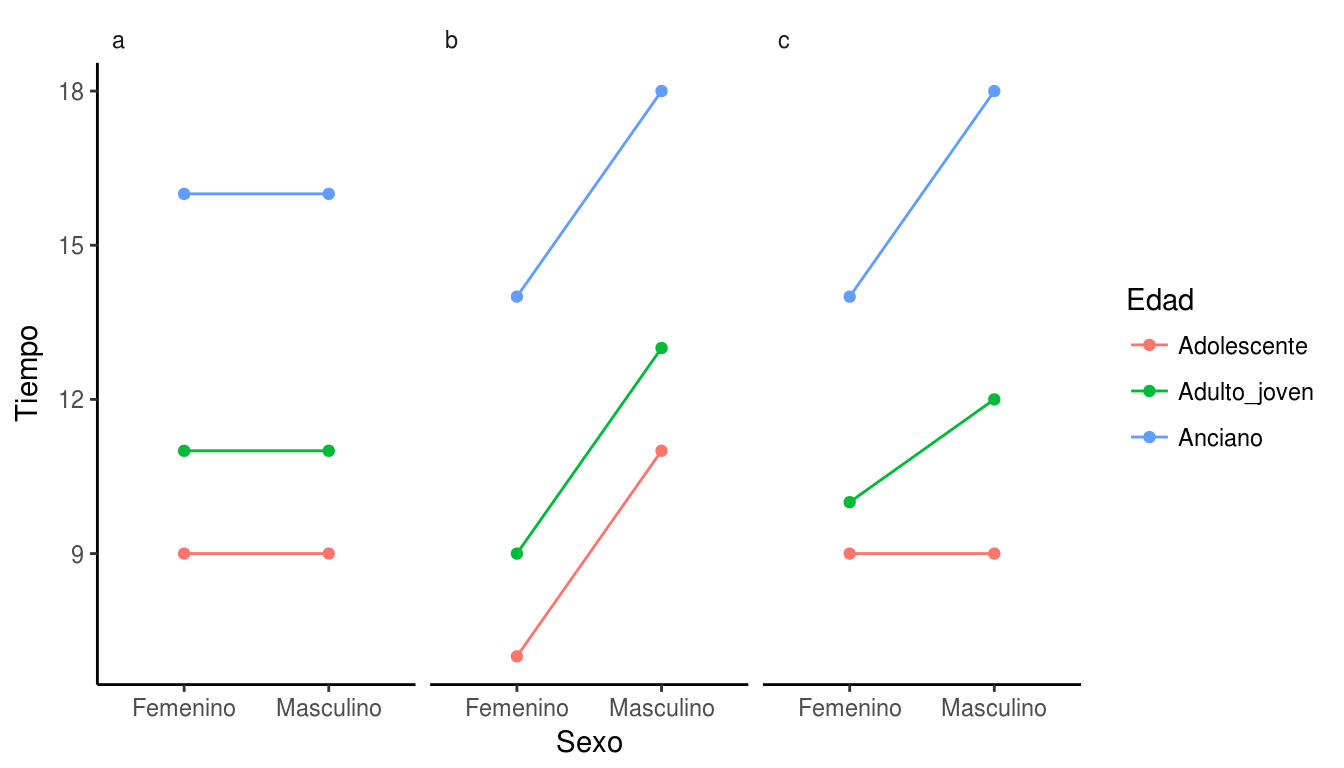
\includegraphics{anova-dos-factores_files/figure-latex/interaccion1-1.pdf}
\includegraphics{anova-dos-factores_files/figure-latex/interaccion1-2.pdf}

\begin{longtable}[]{@{}lllll@{}}
\caption{\label{tab:aprendizaje2} Tiempo de aprendizaje (en minutos) en
mujeres de y hombres de tres edades. Caso sin interacción y efecto del
factor \emph{Sexo}.}\tabularnewline
\toprule
\begin{minipage}[b]{0.15\columnwidth}\raggedright
SEXO\strut
\end{minipage} & \begin{minipage}[b]{0.17\columnwidth}\raggedright
EDAD\strut
\end{minipage} & \begin{minipage}[b]{0.17\columnwidth}\raggedright
\strut
\end{minipage} & \begin{minipage}[b]{0.16\columnwidth}\raggedright
\strut
\end{minipage} & \begin{minipage}[b]{0.20\columnwidth}\raggedright
\strut
\end{minipage}\tabularnewline
\midrule
\endfirsthead
\toprule
\begin{minipage}[b]{0.15\columnwidth}\raggedright
SEXO\strut
\end{minipage} & \begin{minipage}[b]{0.17\columnwidth}\raggedright
EDAD\strut
\end{minipage} & \begin{minipage}[b]{0.17\columnwidth}\raggedright
\strut
\end{minipage} & \begin{minipage}[b]{0.16\columnwidth}\raggedright
\strut
\end{minipage} & \begin{minipage}[b]{0.20\columnwidth}\raggedright
\strut
\end{minipage}\tabularnewline
\midrule
\endhead
\begin{minipage}[t]{0.15\columnwidth}\raggedright
\strut
\end{minipage} & \begin{minipage}[t]{0.17\columnwidth}\raggedright
\textbf{Adolescente (\(j = 1\))}\strut
\end{minipage} & \begin{minipage}[t]{0.17\columnwidth}\raggedright
\textbf{Adulto joven (\(j = 2\))}\strut
\end{minipage} & \begin{minipage}[t]{0.16\columnwidth}\raggedright
\textbf{Anciano (\(j = 3\)) }\strut
\end{minipage} & \begin{minipage}[t]{0.20\columnwidth}\raggedright
\textbf{\(\mu_{i\bullet}\)}\strut
\end{minipage}\tabularnewline
\begin{minipage}[t]{0.15\columnwidth}\raggedright
\textbf{Masculino (\(i = 1\))}\strut
\end{minipage} & \begin{minipage}[t]{0.17\columnwidth}\raggedright
11 (\(\mu_{11}\))\strut
\end{minipage} & \begin{minipage}[t]{0.17\columnwidth}\raggedright
13 (\(\mu_{12}\))\strut
\end{minipage} & \begin{minipage}[t]{0.16\columnwidth}\raggedright
18 (\(\mu_{13}\))\strut
\end{minipage} & \begin{minipage}[t]{0.20\columnwidth}\raggedright
14 (\(\mu_{1 \bullet}\))\strut
\end{minipage}\tabularnewline
\begin{minipage}[t]{0.15\columnwidth}\raggedright
\textbf{Femenino (\(i = 2\))}\strut
\end{minipage} & \begin{minipage}[t]{0.17\columnwidth}\raggedright
7 (\(\mu_{21}\))\strut
\end{minipage} & \begin{minipage}[t]{0.17\columnwidth}\raggedright
9 (\(\mu_{22}\))\strut
\end{minipage} & \begin{minipage}[t]{0.16\columnwidth}\raggedright
14 (\(\mu_{23}\))\strut
\end{minipage} & \begin{minipage}[t]{0.20\columnwidth}\raggedright
10 (\(\mu_{2 \bullet}\))\strut
\end{minipage}\tabularnewline
\begin{minipage}[t]{0.15\columnwidth}\raggedright
\textbf{\(\mu_{\bullet j}\)}\strut
\end{minipage} & \begin{minipage}[t]{0.17\columnwidth}\raggedright
9 (\(\mu_{\bullet 1}\))\strut
\end{minipage} & \begin{minipage}[t]{0.17\columnwidth}\raggedright
11 (\(\mu_{\bullet 2}\))\strut
\end{minipage} & \begin{minipage}[t]{0.16\columnwidth}\raggedright
16 (\(\mu_{\bullet 3}\))\strut
\end{minipage} & \begin{minipage}[t]{0.20\columnwidth}\raggedright
12 (\(\mu_{\bullet \bullet}\))\strut
\end{minipage}\tabularnewline
\bottomrule
\end{longtable}

\hypertarget{interaccion}{%
\section{Interacción}\label{interaccion}}

\[
\mu_{ij} = \mu_{\bullet\bullet} + \alpha_i + \beta_j
\] Si esto se cumple, los efectos serán aditivos; de lo contrario los
factores interactúan.

\begin{longtable}[]{@{}llllll@{}}
\caption{\label{tab:aprendizaje3} Tiempo de aprendizaje (en minutos) en
mujeres de y hombres de tres edades. Caso con
interacción.}\tabularnewline
\toprule
\begin{minipage}[b]{0.12\columnwidth}\raggedright
SEXO\strut
\end{minipage} & \begin{minipage}[b]{0.19\columnwidth}\raggedright
EDAD\strut
\end{minipage} & \begin{minipage}[b]{0.13\columnwidth}\raggedright
\strut
\end{minipage} & \begin{minipage}[b]{0.12\columnwidth}\raggedright
\strut
\end{minipage} & \begin{minipage}[b]{0.16\columnwidth}\raggedright
\strut
\end{minipage} & \begin{minipage}[b]{0.11\columnwidth}\raggedright
\strut
\end{minipage}\tabularnewline
\midrule
\endfirsthead
\toprule
\begin{minipage}[b]{0.12\columnwidth}\raggedright
SEXO\strut
\end{minipage} & \begin{minipage}[b]{0.19\columnwidth}\raggedright
EDAD\strut
\end{minipage} & \begin{minipage}[b]{0.13\columnwidth}\raggedright
\strut
\end{minipage} & \begin{minipage}[b]{0.12\columnwidth}\raggedright
\strut
\end{minipage} & \begin{minipage}[b]{0.16\columnwidth}\raggedright
\strut
\end{minipage} & \begin{minipage}[b]{0.11\columnwidth}\raggedright
\strut
\end{minipage}\tabularnewline
\midrule
\endhead
\begin{minipage}[t]{0.12\columnwidth}\raggedright
\strut
\end{minipage} & \begin{minipage}[t]{0.19\columnwidth}\raggedright
\textbf{Adolescente (\(j = 1\))}\strut
\end{minipage} & \begin{minipage}[t]{0.13\columnwidth}\raggedright
\textbf{Adulto joven (\(j = 2\))}\strut
\end{minipage} & \begin{minipage}[t]{0.12\columnwidth}\raggedright
\textbf{Anciano (\(j = 3\))}\strut
\end{minipage} & \begin{minipage}[t]{0.16\columnwidth}\raggedright
\textbf{\(\mu_{i\bullet}\)}\strut
\end{minipage} & \begin{minipage}[t]{0.11\columnwidth}\raggedright
\strut
\end{minipage}\tabularnewline
\begin{minipage}[t]{0.12\columnwidth}\raggedright
\textbf{Masculino (\(i = 1\))}\strut
\end{minipage} & \begin{minipage}[t]{0.19\columnwidth}\raggedright
9 (\(\mu_{11}\))\strut
\end{minipage} & \begin{minipage}[t]{0.13\columnwidth}\raggedright
12 (\(\mu_{12}\))\strut
\end{minipage} & \begin{minipage}[t]{0.12\columnwidth}\raggedright
18 (\(\mu_{13}\))\strut
\end{minipage} & \begin{minipage}[t]{0.16\columnwidth}\raggedright
13 (\(\mu_{1 \bullet}\))\strut
\end{minipage} & \begin{minipage}[t]{0.11\columnwidth}\raggedright
1( \(\alpha_{1}\))\strut
\end{minipage}\tabularnewline
\begin{minipage}[t]{0.12\columnwidth}\raggedright
\textbf{Femenino (\(i = 2\))}\strut
\end{minipage} & \begin{minipage}[t]{0.19\columnwidth}\raggedright
9 (\(\mu_{21}\))\strut
\end{minipage} & \begin{minipage}[t]{0.13\columnwidth}\raggedright
10 (\(\mu_{22}\))\strut
\end{minipage} & \begin{minipage}[t]{0.12\columnwidth}\raggedright
14 (\(\mu_{23}\))\strut
\end{minipage} & \begin{minipage}[t]{0.16\columnwidth}\raggedright
11 (\(\mu_{2 \bullet}\))\strut
\end{minipage} & \begin{minipage}[t]{0.11\columnwidth}\raggedright
-1 (\(\alpha_{2}\))\strut
\end{minipage}\tabularnewline
\begin{minipage}[t]{0.12\columnwidth}\raggedright
\textbf{\(\mu_{\bullet j}\)}\strut
\end{minipage} & \begin{minipage}[t]{0.19\columnwidth}\raggedright
9 (\(\mu_{\bullet 1}\))\strut
\end{minipage} & \begin{minipage}[t]{0.13\columnwidth}\raggedright
11 (\(\mu_{\bullet 2}\))\strut
\end{minipage} & \begin{minipage}[t]{0.12\columnwidth}\raggedright
16 (\(\mu_{\bullet 3}\))\strut
\end{minipage} & \begin{minipage}[t]{0.16\columnwidth}\raggedright
12 (\(\mu_{\bullet \bullet}\))\strut
\end{minipage} & \begin{minipage}[t]{0.11\columnwidth}\raggedright
\strut
\end{minipage}\tabularnewline
\begin{minipage}[t]{0.12\columnwidth}\raggedright
\strut
\end{minipage} & \begin{minipage}[t]{0.19\columnwidth}\raggedright
-3 (\(\beta_{1}\))\strut
\end{minipage} & \begin{minipage}[t]{0.13\columnwidth}\raggedright
-1 (\(\beta_{2}\))\strut
\end{minipage} & \begin{minipage}[t]{0.12\columnwidth}\raggedright
4 (\(\beta_{3}\))\strut
\end{minipage} & \begin{minipage}[t]{0.16\columnwidth}\raggedright
\strut
\end{minipage} & \begin{minipage}[t]{0.11\columnwidth}\raggedright
\strut
\end{minipage}\tabularnewline
\bottomrule
\end{longtable}

Para el ejemplo de la tabla, es claro que los efectos de los factores
interactúan, por ejemplo:

\[
\mu_{\bullet \bullet} + \alpha_{1} + \beta_{1} = 12 + 1 + ( - 3) = 10
\]

mientras que \(\mu_{11} = 9\).

La diferencia entre la media del tratamiento \(\mu_{ij}\) y el valor
(\(\mu_{\bullet \bullet} + \alpha_{i} + \beta_{j}\)) es llamada la
\emph{interacción} del i-ésimo nivel del factor \(A\) con el j-ésimo
nivel del factor \(B\), se simboliza \(\left( \alpha\beta \right)_{ij}\)
y la definimos como:

\[
\left( \alpha\beta \right)_{ij} = \mu_{ij} - (\mu_{\bullet \bullet} + \alpha_{i} + \beta_{j})
\]

Reemplazando \(\alpha_{i}\) y \(\beta_{j}\) por su definición, se
obtiene la siguiente expresión alternativa:

\[
\left( \alpha\beta \right)_{ij} = \mu_{ij} - \mu_{I \bullet} - \mu_{\bullet j} + \mu_{\bullet \bullet}
\]

Por ejemplo, la interacción para:

\[
\begin{aligned}
\left( \alpha\beta \right)_{13}& = \mu_{13}\left( \mu_{\bullet \bullet} + \alpha_{1} + \beta_{3} \right) \\
& = 18\left( 12 + 1 + 4 \right) \\
& = 1 \\
\end{aligned}
\]

\begin{longtable}[]{@{}lllll@{}}
\caption{\label{tab:efectos} Efectos de
\(\alpha \beta_{ij}\).}\tabularnewline
\toprule
& \(j = 1\) & \(j = 2\) & \(j = 3\) & Promedio\tabularnewline
\midrule
\endfirsthead
\toprule
& \(j = 1\) & \(j = 2\) & \(j = 3\) & Promedio\tabularnewline
\midrule
\endhead
\(i = 1\) & -1 & 0 & 1 & 0\tabularnewline
\(i = 2\) & 1 & 0 & -1 & 0\tabularnewline
Promedio & 0 & 0 & 0 & 0\tabularnewline
\bottomrule
\end{longtable}

\hypertarget{interacciones-no-importantes}{%
\subsection{Interacciones no
importantes}\label{interacciones-no-importantes}}

Muchas veces se detectan interacciones pero estas son pequeñas y no
cambian las conclusiones que se pueden sacar sobre el efecto de los
factores principales.

\begin{longtable}[]{@{}lllll@{}}
\caption{\label{tab:aprendizaje4} Tiempo de aprendizaje (en minutos) en
mujeres de y hombres de tres edades. Caso con interacción no
importante.}\tabularnewline
\toprule
\begin{minipage}[b]{0.15\columnwidth}\raggedright
SEXO\strut
\end{minipage} & \begin{minipage}[b]{0.17\columnwidth}\raggedright
EDAD\strut
\end{minipage} & \begin{minipage}[b]{0.17\columnwidth}\raggedright
\strut
\end{minipage} & \begin{minipage}[b]{0.16\columnwidth}\raggedright
\strut
\end{minipage} & \begin{minipage}[b]{0.20\columnwidth}\raggedright
\strut
\end{minipage}\tabularnewline
\midrule
\endfirsthead
\toprule
\begin{minipage}[b]{0.15\columnwidth}\raggedright
SEXO\strut
\end{minipage} & \begin{minipage}[b]{0.17\columnwidth}\raggedright
EDAD\strut
\end{minipage} & \begin{minipage}[b]{0.17\columnwidth}\raggedright
\strut
\end{minipage} & \begin{minipage}[b]{0.16\columnwidth}\raggedright
\strut
\end{minipage} & \begin{minipage}[b]{0.20\columnwidth}\raggedright
\strut
\end{minipage}\tabularnewline
\midrule
\endhead
\begin{minipage}[t]{0.15\columnwidth}\raggedright
\strut
\end{minipage} & \begin{minipage}[t]{0.17\columnwidth}\raggedright
\textbf{Adolescente (\(j = 1\))}\strut
\end{minipage} & \begin{minipage}[t]{0.17\columnwidth}\raggedright
\textbf{Adulto joven (\(j = 2\))}\strut
\end{minipage} & \begin{minipage}[t]{0.16\columnwidth}\raggedright
\textbf{Anciano (\(j = 3\)) }\strut
\end{minipage} & \begin{minipage}[t]{0.20\columnwidth}\raggedright
\textbf{\(\mu_{i\bullet}\)}\strut
\end{minipage}\tabularnewline
\begin{minipage}[t]{0.15\columnwidth}\raggedright
\textbf{Masculino (\(i = 1\))}\strut
\end{minipage} & \begin{minipage}[t]{0.17\columnwidth}\raggedright
9.75 (\(\mu_{11}\))\strut
\end{minipage} & \begin{minipage}[t]{0.17\columnwidth}\raggedright
12 (\(\mu_{12}\))\strut
\end{minipage} & \begin{minipage}[t]{0.16\columnwidth}\raggedright
17.25 (\(\mu_{13}\))\strut
\end{minipage} & \begin{minipage}[t]{0.20\columnwidth}\raggedright
14 (\(\mu_{1 \bullet}\))\strut
\end{minipage}\tabularnewline
\begin{minipage}[t]{0.15\columnwidth}\raggedright
\textbf{Femenino (\(i = 2\))}\strut
\end{minipage} & \begin{minipage}[t]{0.17\columnwidth}\raggedright
8.25 (\(\mu_{21}\))\strut
\end{minipage} & \begin{minipage}[t]{0.17\columnwidth}\raggedright
10 (\(\mu_{22}\))\strut
\end{minipage} & \begin{minipage}[t]{0.16\columnwidth}\raggedright
14.75 (\(\mu_{23}\))\strut
\end{minipage} & \begin{minipage}[t]{0.20\columnwidth}\raggedright
10 (\(\mu_{2 \bullet}\))\strut
\end{minipage}\tabularnewline
\begin{minipage}[t]{0.15\columnwidth}\raggedright
\textbf{\(\mu_{\bullet j}\)}\strut
\end{minipage} & \begin{minipage}[t]{0.17\columnwidth}\raggedright
9 (\(\mu_{\bullet 1}\))\strut
\end{minipage} & \begin{minipage}[t]{0.17\columnwidth}\raggedright
11 (\(\mu_{\bullet 2}\))\strut
\end{minipage} & \begin{minipage}[t]{0.16\columnwidth}\raggedright
16 (\(\mu_{\bullet 3}\))\strut
\end{minipage} & \begin{minipage}[t]{0.20\columnwidth}\raggedright
12 (\(\mu_{\bullet \bullet}\))\strut
\end{minipage}\tabularnewline
\bottomrule
\end{longtable}





\begin{figure}
\includegraphics[width=0.5\linewidth]{anova-dos-factores_files/figure-latex/interaccion-no-importante-1} \includegraphics[width=0.5\linewidth]{anova-dos-factores_files/figure-latex/interaccion-no-importante-2} \caption{Gráfico de interacción para las medias
del tiempo de aprendizaje. Los datos graficados corresponden a la Tabla
\ref{tab:aprendizaje4}}\label{fig:interaccion-no-importante}
\end{figure}

\hypertarget{interacciones-transformables-y-no-transformables}{%
\subsubsection{Interacciones transformables y no
transformables}\label{interacciones-transformables-y-no-transformables}}

\emph{Efectos de los factores multiplicativos}

Consideremos el caso donde los efectos de los factores son
multiplicativos, en lugar de aditivos:

\(\mu_{ij} = \mu_{\bullet \bullet}\alpha_{i}\beta_{j}\)

Estas interacciones pueden ser eliminadas aplicando la transformación
logarítmica:

\[
\log(\mu_{ij}) = \log(\mu_{\bullet \bullet}) + \log(\alpha_{i}) + \log(\beta_{j})
\]

o sea

\[
{u'}_{ij} = {u'}_{\bullet \bullet} + \alpha_{i}^{'} + \beta_{j}^{'}
\]

\[
\begin{matrix}
\mu_{ij}^{'} = log \mu_{ij} & \mu_{\bullet \bullet}^{'} = log \mu_{\bullet \bullet} & \alpha_{i}^{'} = \log\alpha_{i} & \beta_{j}^{'} = \log\beta_{j}
\end{matrix}
\]

Entonces se usa la variable \(Y' = \log Y\)

Cuando una simple transformación de Y remueve los efectos de la
interacción o los hace poco importantes, decimos que la interacción es
\emph{transformable}.

\emph{Interacciones multiplicativas}

Otro ejemplo de interacciones transformables aparece cuando cada efecto
de interacción es igual al producto de funciones de los efectos
principales.

\[
\mu_{ij} = \alpha_{i} + \beta_{j} + 2\sqrt{\alpha_{i}}\sqrt{\beta_{j}}
\]

o lo que es lo mismo

\[
\mu_{ij} = \left( \sqrt{\alpha_{i}}\sqrt{\beta_{j}} \right)^{2}
\]

Si se aplica la transformación raíz cuadrada, se obtiene:

\[
\mu_{ij}^{'} = \alpha_{i}^{'} + \beta_{j}^{'}
\]

donde:

\[
\begin{matrix}
{u^{'}}_{ij} = \sqrt{\mu_{ij}} & \alpha_{i}^{'} = \sqrt{\alpha_{i}} & \beta_{j}^{'} = \sqrt{\beta_{i}} \\
\end{matrix}
\]

Las transformaciones que convierten las interacciones importantes en no
importantes son: cuadrado, raíz cuadrada, logaritmo y recíproca.

\begin{longtable}[]{@{}lll@{}}
\caption{\label{tab:ejemplo-transformaciones} Ejemplo de transformacion de
medias de tratamientos: a) Medias de tratamientos escala original b)
Medias de tratamientos después de la transformación
\(\sqrt{}\)}\tabularnewline
\toprule
factor \(A\) & factor \(B\) &\tabularnewline
\midrule
\endfirsthead
\toprule
factor \(A\) & factor \(B\) &\tabularnewline
\midrule
\endhead
& \(j = 1\) & \(j = 2\)\tabularnewline
\(i = 1\) & 16 & 64\tabularnewline
\(i = 2\) & 49 & 121\tabularnewline
\(i = 3\) & 64 & 144\tabularnewline
\bottomrule
\end{longtable}

\begin{longtable}[]{@{}lll@{}}
\toprule
factor \(A\) & factor \(B\) &\tabularnewline
\midrule
\endhead
& \(j = 1\) & \(j = 2\)\tabularnewline
\(i = 1\) & 4 & 8\tabularnewline
\(i = 2\) & 7 & 11\tabularnewline
\(i = 3\) & 8 & 12\tabularnewline
\bottomrule
\end{longtable}

\hypertarget{modelo-i-para-estudios-de-dos-factores}{%
\section{MODELO I PARA ESTUDIOS DE DOS
FACTORES}\label{modelo-i-para-estudios-de-dos-factores}}

El factor \(A\) es estudiado en \(I\) niveles, y estos no representan
una muestra aleatoria de todos los niveles posibles de \(A\). De manera
equivalente el factor \(B\) se estudia sobre \(J\) niveles. Todas las
\(IJ\) combinaciones de los niveles de los factores son incluidas en el
análisis. El número de casos para cada uno de los \(IJ\) tratamientos es
el mismo, lo indicamos con \(n\), y es necesario que \(n > 1\). Entonces
el número total de casos es:

\[
N  =  IJn
\]

\hypertarget{modelo-de-las-medias-de-celdas}{%
\subsection{Modelo de las medias de
celdas}\label{modelo-de-las-medias-de-celdas}}

Se puede expresar el modelo de niveles del factor fijos en términos de
las medias de los tratamientos.

\[
Y_{ijk} = \mu_{ij} + \varepsilon_{ijk}
\]

\[
i = 1,2,\ldots,I;j = 1,2,\ldots,J;k = 1,2,\ldots,n
\]

\hypertarget{caracteristicas-importantes-del-modelo-2}{%
\subsubsection{Características importantes del
Modelo}\label{caracteristicas-importantes-del-modelo-2}}

\begin{enumerate}
\def\labelenumi{\arabic{enumi}.}
\item
  \(E(Y_{ijk}) = \mu_{ij}\)
\item
  \(Var(Y_{ijk}) = Var(\varepsilon_{ijk}) = \sigma^{2}\)
\item
  \(Y_ijk\) son independientes y se distribuyen
  \(N\left( 0,\sigma^{2} \right)\)
\item
  El modelo de ANOVA es un modelo lineal.
\item
  El modelo de ANOVA de dos factores es similar al de un factor.
  Normalidad, independencia de los términos del error y constancia de la
  varianza para los términos del error son propiedades de ambos modelos.
\end{enumerate}

\hypertarget{modelo-de-los-efectos-de-los-factores}{%
\subsection{Modelo de los efectos de los
factores}\label{modelo-de-los-efectos-de-los-factores}}

Una forma equivalente de enunciar el modelo se obtiene de la definición
de interacción:

\[
\left( \alpha\beta \right)_{ij} = \mu_{ij}(\mu_{\bullet \bullet} + \alpha_{i} + \beta_{j})
\]

Reordenando términos se obtiene:

\[
\mu_{ij} = \mu_{\bullet \bullet} + \alpha_{i} + \beta_{j} + \left( \alpha\beta \right)_{ij}
\]

donde:

\[
\mu_{\bullet \bullet} = \frac{\sum_{i = 1}^{I}{\sum_{j = 1}^{J}\mu_{ij}}}{IJ}
\]

\[
\alpha_{i} = \mu_{i \bullet} - \mu_{\bullet \bullet}
\]

\[
\beta_{j} = \mu_{\bullet j} - \mu_{\bullet \bullet}
\]

\[
\left( \alpha\beta \right)_{ij} = \mu_{ij} - \mu_{i \bullet} - \mu_{\bullet j} - \mu_{\bullet \bullet}
\]

La media de la celda µij para cualquier tratamiento puede ser vista como
la suma de cuatro componentes de los efectos de los factores.
Específicamente:

\begin{enumerate}
\def\labelenumi{\arabic{enumi}.}
\item
  Una constante general \(\mu_{\bullet \bullet}\).
\item
  El efecto principal \(\alpha_{i}\) del factor \(A\) en el i-ésimo
  nivel.
\item
  El efecto principal \(\beta_{j}\) del factor \(B\) en el j-ésimo
  nivel.
\item
  El efecto de la interacción \(\left( \alpha\beta \right)_{ij}\)
\end{enumerate}

Reemplazando \(\mu_{ij}\) en el modelo de las medias de las celdas, se
obtiene:

\[
Y_{ijk} = \mu_{\bullet \bullet} + \alpha_{i} + \beta_{j} + \left( \alpha\beta \right)_{ij} + \varepsilon_{ijk}
\]

donde:

\(\mu_{\bullet \bullet}\) es una constante\\
\(\alpha_{i}\) son constantes sujetas a la restricción
\(\sum\alpha_{i} = 0\)\\
\(\beta_{j}\) son constantes sujetas a la restricción
\(\sum\beta_{j} = 0\)\\
\(\left( \alpha\beta \right)_{ij}\) son constantes sujetas a las
restricciones

\[
\begin{matrix}
\sum_{i}^{I}\left( \alpha\beta \right)_{ij} = 0 & \sum_{j}^{J}\left( \alpha\beta \right)_{ij} = 0 \\
\end{matrix}
\]

\(\varepsilon_{ijk}\) son independientes y se distribuyen \(N(0,\
\sigma^{2})\)

\hypertarget{anova-modelo-i}{%
\subsection{ANOVA (MODELO I)}\label{anova-modelo-i}}

\hypertarget{notacion}{%
\subsubsection{Notación}\label{notacion}}

\[
\overline{Y}_{ij \bullet} = \frac{\sum_{k = 1}^{n}Y_{ijk}}{n}
\]

\[
\overline{Y}_{i \bullet \bullet} = \frac{\sum_{j}^{J}{\sum_{k = 1}^{n}Y_{ijk}}}{\text{Jn}}
\]

\[
\overline{Y}_{\bullet j \bullet} = \frac{\sum_{i}^{I}{\sum_{k = 1}^{n}Y_{ijk}}}{\text{In}}
\]

\[
\overline{Y}_{\bullet \bullet \bullet} = \frac{\sum_{i}^{I}{\sum_{j}^{J}{\sum_{k = 1}^{n}Y_{ijk}}}}{\text{IJn}}
\]

\hypertarget{ajuste-del-modelo}{%
\subsubsection{Ajuste del modelo}\label{ajuste-del-modelo}}

\hypertarget{modelo-de-las-medias-de-celda}{%
\paragraph{Modelo de las medias de
celda}\label{modelo-de-las-medias-de-celda}}

El cuadrado a minimizar es el siguiente:

\[
\sum\sum\sum\left( Y_{ijk} - \mu_{ij} \right)^{2}
\]

Minimizando se obtiene:

\[
\hat{\mu}_{ij} = \overline{Y}_{ij \bullet}
\]

Los residuos se definen como la diferencia entre los valores observados
y los estimados:

\[
\varepsilon_{ijk} = Y_{ijk} - \overline{Y}_{ij \bullet}
\]

\hypertarget{modelo-de-los-efectos-del-factor}{%
\paragraph{Modelo de los efectos del
factor}\label{modelo-de-los-efectos-del-factor}}

El cuadrado a minimizar es el siguiente:

\[
\sum\sum\sum\left( Y_{ijk} - \mu_{\bullet \bullet} - \alpha_{i} - \beta_{j} - \left( \alpha\beta \right)_{ij} \right)^{2}
\]

sujeto a las restricciones:

\[
\begin{matrix}
\sum_{i}^{I}\alpha_{i} = 0 & \sum_{j}^{J}\beta_{j} = 0 & \sum_{i}^{I}\left( \alpha\beta \right)_{ij} = 0 & \sum_{j}^{J}\left( \alpha\beta \right)_{ij} = 0 \\
\end{matrix}
\]

Cuando se minimiza se obtienen los siguientes estimadores de mínimos
cuadrados:

\begin{longtable}[]{@{}ll@{}}
\toprule
\begin{minipage}[b]{0.35\columnwidth}\raggedright
Parámetro\strut
\end{minipage} & \begin{minipage}[b]{0.59\columnwidth}\raggedright
Estimador\strut
\end{minipage}\tabularnewline
\midrule
\endhead
\begin{minipage}[t]{0.35\columnwidth}\raggedright
\(\mu_{\bullet \bullet}\)\strut
\end{minipage} & \begin{minipage}[t]{0.59\columnwidth}\raggedright
\({\overline{Y}_{\bullet \bullet \bullet}}\)\strut
\end{minipage}\tabularnewline
\begin{minipage}[t]{0.35\columnwidth}\raggedright
\(\alpha_{i} = \mu_{i \bullet} - \mu_{\bullet \bullet}\)\strut
\end{minipage} & \begin{minipage}[t]{0.59\columnwidth}\raggedright
\(\overline{Y}_{i \bullet \bullet} - \overline{Y}_{\bullet \bullet \bullet}\)\strut
\end{minipage}\tabularnewline
\begin{minipage}[t]{0.35\columnwidth}\raggedright
\(\beta_{j} = \mu_{\bullet j} - \mu_{\bullet \bullet}\)\strut
\end{minipage} & \begin{minipage}[t]{0.59\columnwidth}\raggedright
\(\overline{Y}_{\bullet j \bullet} - \overline{Y}_{\bullet \bullet \bullet}\)\strut
\end{minipage}\tabularnewline
\begin{minipage}[t]{0.35\columnwidth}\raggedright
\(\left( \alpha\beta \right)_{ij} = \mu_{ij} - \mu_{i \bullet} - \mu_{\bullet j} + \mu_{\bullet \bullet}\)\strut
\end{minipage} & \begin{minipage}[t]{0.59\columnwidth}\raggedright
\(\overline{Y}_{ij \bullet} - \overline{Y}_{i \bullet \bullet} - \overline{Y}_{\bullet j \bullet} + \overline{Y}_{\bullet \bullet \bullet}\)\strut
\end{minipage}\tabularnewline
\bottomrule
\end{longtable}

\hypertarget{descomposicion-de-la-suma-de-cuadrados-total}{%
\paragraph{Descomposición de la suma de cuadrados
total}\label{descomposicion-de-la-suma-de-cuadrados-total}}

Para una observación, se puede descomponer la desviación con respecto a
la media total, en dos partes:

\[
\begin{matrix}
\underbrace{\left ( Y_{ijk}-\overline{Y}_{\bullet\bullet\bullet} \right )} & = & \underbrace{\left ( \overline{Y}_{ij\bullet}-\overline{Y}_{\bullet\bullet\bullet} \right )}& + & \underbrace{\left ( Y_{ijk}-\overline{Y}_{ij\bullet} \right )}\\
\text{Desviacion Total} & & \text{Desviacion de los tratamientos} & & \text{Desviacion de las observaciones}  \\
\end{matrix}
\]

También se puede descomponer la desviación estimada de la media de los
tratamientos en:

\[
\begin{matrix}
  \underbrace{\overline{Y}_{ij\bullet} - \overline{Y}_{\bullet \bullet \bullet}}& = & \underbrace{\overline{Y}_{i\bullet\bullet} - \overline{Y}_{\bullet \bullet \bullet}} & + & \underbrace{\overline{Y}_{\bullet j \bullet} - \overline{Y}_{\bullet \bullet \bullet}} & + & \underbrace{\overline{Y}_{ij \bullet} - \overline{Y}_{i \bullet \bullet} - \overline{Y}_{\bullet j \bullet} + \overline{Y}_{\bullet \bullet \bullet}} \\
\text{Desviacion de} & & \text{Efecto principal} & & \text{Efecto principal} & & \text{Efecto de}  \\
\text{ los tratamientos} & & \text{A} & & \text{B} & & \text{ la interaccion}
\end{matrix}
\]

\#\#\#TABLA DE ANOVA PARA DOS FACTORES. MODELO I

\emph{Más de una observación por celda}

\begin{longtable}[]{@{}lllll@{}}
\toprule
\begin{minipage}[b]{0.04\columnwidth}\raggedright
Fuente de variación\strut
\end{minipage} & \begin{minipage}[b]{0.29\columnwidth}\raggedright
SC\strut
\end{minipage} & \begin{minipage}[b]{0.02\columnwidth}\raggedright
GL\strut
\end{minipage} & \begin{minipage}[b]{0.13\columnwidth}\raggedright
CM\strut
\end{minipage} & \begin{minipage}[b]{0.37\columnwidth}\raggedright
E(CM)\strut
\end{minipage}\tabularnewline
\midrule
\endhead
\begin{minipage}[t]{0.04\columnwidth}\raggedright
Entre tratamientos\strut
\end{minipage} & \begin{minipage}[t]{0.29\columnwidth}\raggedright
\(SC_{E} = n\sum_{ij}^{}\overline{Y}_{ij \bullet}^{2} - N\overline{Y}_{\bullet \bullet \bullet}^{2}\)\strut
\end{minipage} & \begin{minipage}[t]{0.02\columnwidth}\raggedright
\(IJ-1\)\strut
\end{minipage} & \begin{minipage}[t]{0.13\columnwidth}\raggedright
\(\frac{SC_{E}}{IJ-1}\)\strut
\end{minipage} & \begin{minipage}[t]{0.37\columnwidth}\raggedright
\(\sigma^{2} + \frac{n}{IJ - 1}\sum\sum\left( \mu_{ij} - \mu_{\bullet \bullet} \right)^{2}\)\strut
\end{minipage}\tabularnewline
\begin{minipage}[t]{0.04\columnwidth}\raggedright
A\strut
\end{minipage} & \begin{minipage}[t]{0.29\columnwidth}\raggedright
\(SC_{A} = Jn\sum_{i}^{}\overline{Y}_{i \bullet \bullet}^{2} - N\overline{Y}_{\bullet \bullet \bullet}^{2}\)\strut
\end{minipage} & \begin{minipage}[t]{0.02\columnwidth}\raggedright
\(I-1\)\strut
\end{minipage} & \begin{minipage}[t]{0.13\columnwidth}\raggedright
\(\frac{SC_{A}}{I-1}\)\strut
\end{minipage} & \begin{minipage}[t]{0.37\columnwidth}\raggedright
\(\sigma^{2} + \frac{\text{Jn}}{I - 1}\sum\left( \mu_{i \bullet} - \mu_{\bullet \bullet} \right)^{2}\)\strut
\end{minipage}\tabularnewline
\begin{minipage}[t]{0.04\columnwidth}\raggedright
B\strut
\end{minipage} & \begin{minipage}[t]{0.29\columnwidth}\raggedright
\(SC_{B} = In\sum_{j}^{}\overline{Y}_{\bullet j \bullet}^{2} - N\overline{Y}_{\bullet \bullet \bullet}^{2}\)\strut
\end{minipage} & \begin{minipage}[t]{0.02\columnwidth}\raggedright
\(J-1\)\strut
\end{minipage} & \begin{minipage}[t]{0.13\columnwidth}\raggedright
\(\frac{SC_{B}}{J-1}\)\strut
\end{minipage} & \begin{minipage}[t]{0.37\columnwidth}\raggedright
\(\sigma^{2} + \frac{\text{In}}{J - 1}\sum\left( \mu_{\bullet j} - \mu_{\bullet \bullet} \right)^{2}\)\strut
\end{minipage}\tabularnewline
\begin{minipage}[t]{0.04\columnwidth}\raggedright
AB (Interacción)\strut
\end{minipage} & \begin{minipage}[t]{0.29\columnwidth}\raggedright
\(SC_{E}-SC_{A} - SC_{B}\)\strut
\end{minipage} & \begin{minipage}[t]{0.02\columnwidth}\raggedright
\((I-1)(J-1)\)\strut
\end{minipage} & \begin{minipage}[t]{0.13\columnwidth}\raggedright
\(\frac{SC_{AB}}{\left( I1 \right)\left( J - 1 \right)}\)\strut
\end{minipage} & \begin{minipage}[t]{0.37\columnwidth}\raggedright
\(\sigma^{2} + \frac{n}{\left( I - 1 \right)\left( J - 1 \right)}\sum\sum\left( \mu_{ij} - \mu_{i \bullet} - \mu_{\bullet j} + \mu_{\bullet \bullet} \right)^{2}\)\strut
\end{minipage}\tabularnewline
\begin{minipage}[t]{0.04\columnwidth}\raggedright
Error\strut
\end{minipage} & \begin{minipage}[t]{0.29\columnwidth}\raggedright
\(SC_{T} - SC_{E}\)\strut
\end{minipage} & \begin{minipage}[t]{0.02\columnwidth}\raggedright
\(N-IJ\)\strut
\end{minipage} & \begin{minipage}[t]{0.13\columnwidth}\raggedright
\(\frac{SC_{D}}{N - IJ}\)\strut
\end{minipage} & \begin{minipage}[t]{0.37\columnwidth}\raggedright
\(\sigma^{2}\)\strut
\end{minipage}\tabularnewline
\begin{minipage}[t]{0.04\columnwidth}\raggedright
Total\strut
\end{minipage} & \begin{minipage}[t]{0.29\columnwidth}\raggedright
\(\sum_{i}^{}{\sum_{j}^{}{\sum_{k}^{}Y_{ijk}^{2}}} - N\overline{Y}_{\bullet \bullet \bullet}^{2}\)\strut
\end{minipage} & \begin{minipage}[t]{0.02\columnwidth}\raggedright
\(N-1\)\strut
\end{minipage} & \begin{minipage}[t]{0.13\columnwidth}\raggedright
\strut
\end{minipage} & \begin{minipage}[t]{0.37\columnwidth}\raggedright
\strut
\end{minipage}\tabularnewline
\bottomrule
\end{longtable}

\hypertarget{prueba-de-f}{%
\section{Prueba de F}\label{prueba-de-f}}

\hypertarget{prueba-para-la-interaccion}{%
\subsubsection{Prueba para la
interacción}\label{prueba-para-la-interaccion}}

\[
\begin{aligned}
H_{0}&:\mu_{ij} - \mu_{i \bullet} - \mu_{\bullet j} + \mu_{\bullet \bullet} = 0\ \forall\ i,j\\
H_{a}&:\mu_{ij} - \mu_{i \bullet} - \mu_{\bullet j} + \mu_{\bullet \bullet} \neq 0\ para\ algun\ i,j
\end{aligned}
\]

o

\[
\begin{aligned}
H_{0}&: \text{todos los } \left( \alpha\beta \right)_{ij}  =  0\\
H_{a}&:\text{no todos los } \left( \alpha\beta \right)_{ij}  =  0
\end{aligned}
\]

La prueba estadística apropiada es:

\[
F^{*} = \frac{CM_{AB}}{CM_{D}}
\]

Recordamos que bajo \(H_{0}\) \(F^{*}\) se distribuye según una
\(F_{1 - \alpha;\left( I-1 \right)\left( J-1 \right),\left( N-IJ \right)}.\)

Entonces:

\begin{itemize}
\item
  Sí
  \(F^{*} \leq F_{1 - \alpha;\left( I-1 \right)\left( J-1 \right),\left( N-IJ \right)}\),
  no se rechaza \(H_{0}\)
\item
  Sí
  \(F^{*} > F_{1 - \alpha;\left( I-1 \right)\left( J-1 \right),\left( N-IJ \right)}\),
  se rechaza \(H_{0}\)
\end{itemize}

\hypertarget{prueba-para-los-efectos-principales}{%
\subsubsection{Prueba para los efectos
principales}\label{prueba-para-los-efectos-principales}}

Estas pruebas se realizan cuando no existe interacción.

Para el factor \(A\):

\[
\begin{aligned}
H_{0}&:\mu_{1 \bullet} = \mu_{2 \bullet} = \ldots = \mu_{I \bullet}\\
H_{a}&:No\ todos\ los\ \mu_{i \bullet}\ \text{son iguales}
\end{aligned}
\]

o

\[
\begin{aligned}
H_{0}:\alpha_{1} = \alpha_{2} = \ldots = \alpha_{I} = 0\\
H_{a}: \text{No todos los } \alpha_{i}\ \text{iguales a cero}
\end{aligned}
\]

Se usa el estadístico

\[
F^{*} = \frac{CM_{A}}{CM_{D}}
\]

Dado que \(F^{*}\), bajo \(H_{0}\), se distribuye según una
\(F_{1 - \alpha;\left( I-1 \right)\left( J-1 \right),\left( N-IJ \right)}.\)

Entonces:

\begin{itemize}
\item
  Sí
  \(F^{*} \leq F_{1 - \alpha;\left( I-1 \right),\left( N-IJ \right)}\),
  no se rechaza \(H_{0}\)
\item
  Sí \(F^{*} > F_{1 - \alpha;\left( I-1 \right),\left( N-IJ \right)}\),
  se rechaza \(H_{0}\)
\end{itemize}

Para el factor \(B\):

\[
\begin{aligned}
H_{0}&:\mu_{\bullet 1} = \mu_{\bullet 2} = \ldots = \mu_{\bullet J}\\
H_{a}&: \text{No todos los } \mu_{\bullet j}\ \text{son iguales}
\end{aligned}
\]

o

\[
\begin{aligned}
H_{0}&:\beta_{1} = \beta_{2} = \ldots = \beta_{J} = 0\\
H_{a}&:\text{No todos los } \beta_{j}\ \text{iguales a cero}
\end{aligned}
\]

El estadístico es

\[
F^{*} = \frac{CM_{B}}{CM_{D}}
\]

y la regla de decisión es:

\begin{itemize}
\item
  Sí
  \(F^{*} \leq F_{1 - \alpha;\left( J-1 \right),\left( N- IJ\right)}\),
  no se rechaza \(H_{0}\)
\item
  Sí \(F^{*} > F_{1 - \alpha;\left( J-1 \right),\left( N- IJ\right)}\),
  se rechaza \(H_{0}\)
\end{itemize}

\emph{Ejemplo}: El asma bronquial es una enfermedad alérgica cuya
virulencia depende de la estación. Se desea comparar tres fármacos
antihistamínicos A, B y C, en las cuatro estaciones del año. Se toma una
muestra de 48 personas con asma crónico de intensidad análoga, que se
divide en 12 grupos, uno para cada fármaco y estación, a razón de 4
enfermos por grupo. Los resultados se evaluaron en una escala objetiva
que iba de 100, y fueron los siguientes:

\begin{longtable}[]{@{}llll@{}}
\toprule
Estación & Fármaco A & Fármaco B & Fármaco C\tabularnewline
\midrule
\endhead
Primavera & 23, 28, 32, 18 & 56, 58, 53, 55 & 42, 41, 36,
37\tabularnewline
Verano & 32, 41, 43, 48 & 64, 58, 67, 72 & 51, 53, 55, 60\tabularnewline
Otoño & 18, 16, 21, 10 & 48, 50, 47, 47 & 28, 31, 23, 33\tabularnewline
Invierno & 30, 40, 33, 47 & 60, 61, 63, 59 & 56, 60, 61,
55\tabularnewline
\bottomrule
\end{longtable}

\begin{enumerate}
\def\labelenumi{\alph{enumi})}
\item
  Determinar si existen diferencias entre los fármacos A, B y C y entre
  las estaciones.
\item
  ¿Es significativa la interacción?
\end{enumerate}

\begin{longtable}[]{@{}llllll@{}}
\caption{\label{tab:resumen-asma} Resumen de los datos de tres fármacos
contra el asma en las cuatro estaciones del año.}\tabularnewline
\toprule
Estación & Fármaco & n & Suma & Media & Varianza\tabularnewline
\midrule
\endfirsthead
\toprule
Estación & Fármaco & n & Suma & Media & Varianza\tabularnewline
\midrule
\endhead
Invierno & A & 4 & 150 & 37.500 & 57.666667\tabularnewline
Invierno & B & 4 & 243 & 60.750 & 2.916667\tabularnewline
Invierno & C & 4 & 232 & 58.000 & 8.666667\tabularnewline
Otoño & A & 4 & 65 & 16.250 & 21.583333\tabularnewline
Otoño & B & 4 & 192 & 48.000 & 2.000000\tabularnewline
Otoño & C & 4 & 115 & 28.750 & 18.916667\tabularnewline
Primavera & A & 4 & 101 & 25.250 & 36.916667\tabularnewline
Primavera & B & 4 & 222 & 55.500 & 4.333333\tabularnewline
Primavera & C & 4 & 156 & 39.000 & 8.666667\tabularnewline
Verano & A & 4 & 164 & 41.000 & 44.666667\tabularnewline
Verano & B & 4 & 261 & 65.250 & 34.250000\tabularnewline
Verano & C & 4 & 219 & 54.750 & 14.916667\tabularnewline
Total & A & 16 & 480 & 30.000 & 135.866667\tabularnewline
Total & B & 16 & 918 & 57.375 & 52.650000\tabularnewline
Total & C & 16 & 722 & 45.125 & 160.650000\tabularnewline
\bottomrule
\end{longtable}






\begin{figure}
\centering
\includegraphics{anova-dos-factores_files/figure-latex/graficos-asma-1.pdf}
\caption{\label{fig:graficos-asma}Efecto de tres fármacos contra el asma en las cuatro
estaciones del año. a -- gráfico de cajas y barras para las 4
estaciones, n = 12. b -- gráfico de cajas y barras para los 3 fármacos,
n = 16. c -- gráfico de interacción fármaco x estación, n = 4.}
\end{figure}

\label{tab:anova-asma} Tabla de ANOVA.

\hypertarget{contrastes-1}{%
\section{Contrastes}\label{contrastes-1}}

\hypertarget{entre-filas}{%
\subsection{Entre Filas}\label{entre-filas}}

\[
\hat{f} = \sum c_{i}{\overline{Y}_{i \bullet \bullet}}
\]

\textbf{Bonferroni y Scheffé}

\[
\varepsilon = \frac{\left| \hat{f} \right|}{\sqrt{CM_{D}\left. \ \frac{\sum c_{i}^{2}}{\text{Jn}} \right.\ }\ }
\]

\hypertarget{planeados-1}{%
\subsubsection{Planeados:}\label{planeados-1}}

\hypertarget{bonferroni}{%
\paragraph{Bonferroni}\label{bonferroni}}

\[
VC = t_{1 - \frac{\alpha}{2m};GL_{D}}
\]

\hypertarget{no-planeados-1}{%
\subsubsection{No Planeados:}\label{no-planeados-1}}

\hypertarget{scheffe}{%
\paragraph{Scheffé}\label{scheffe}}

\[
VC = S = \sqrt{\left( I - 1 \right)F_{\left( I - 1 \right);GL_{D};1 - \alpha}}
\]

\hypertarget{tukey}{%
\paragraph{Tukey}\label{tukey}}

\[
\frac{\overline{Y}_{i \bullet \max } - \overline{Y}_{i \bullet \min }}{S_{\overline{Y}}}\sim q_{I;N - IJ}
\]

\[
S_{\overline{y}} = \sqrt{\frac{CM_{D}}{\text{Jn}}}
\]

\hypertarget{ortogonales}{%
\paragraph{Ortogonales}\label{ortogonales}}

\[
SC = \frac{{\hat{f}}^{2}}{\frac{\sum c_{i}^{2}}{\text{Jn}}}\ 
\]

\hypertarget{entre-columnas}{%
\subsection{Entre columnas}\label{entre-columnas}}

\[
\hat{f} = \sum c_{j}{\overline{Y}_{\bullet j \bullet}}
\]

\textbf{Bonferroni y Scheffé}

\[
\varepsilon = \frac{\left| \hat{f} \right|}{\sqrt{CM_{D}\left. \ \frac{\sum c_{j}^{2}}{\text{In}} \right.\ }\ }
\]

\hypertarget{planeados-2}{%
\subsubsection{Planeados:}\label{planeados-2}}

\hypertarget{bonferroni-1}{%
\paragraph{Bonferroni}\label{bonferroni-1}}

\[
VC = t_{1 - \frac{\alpha}{2m};GL_{D}}
\]

\hypertarget{no-planeados-2}{%
\subsubsection{No Planeados:}\label{no-planeados-2}}

\hypertarget{scheffe-1}{%
\paragraph{Scheffé}\label{scheffe-1}}

\[
VC = S = \sqrt{\left( J - 1 \right)F_{\left( J - 1 \right);GL_{D};1 - \alpha}}
\]

\hypertarget{tukey-1}{%
\paragraph{Tukey}\label{tukey-1}}

\[
\frac{\overline{Y}_{\bullet j\ \max } - \overline{Y}_{\bullet j\ \min }}{S_{\overline{Y}}}\sim q_{j;N - IJ}
\]

\[
S_{\overline{Y} = \sqrt{\frac{CM_{D}}{In}}}
\]

\hypertarget{ortogonales-1}{%
\paragraph{Ortogonales}\label{ortogonales-1}}

\[
SC = \frac{{\hat{f}}^{2}}{\frac{\sum c_{j}^{2}}{\text{In}}}\ 
\]

\hypertarget{interaccion-1}{%
\subsection{Interacción}\label{interaccion-1}}

\[
\hat{f} = \sum c_{ij}{\overline{Y}_{ij \bullet}}
\]

Bonferroni y Scheffé

\[
\varepsilon = \frac{\left| \hat{f} \right|}{\sqrt{CM_{D}\left. \ \frac{\sum c_{ij}^{2}}{n} \right.\ }\ }
\]

\hypertarget{planeados-3}{%
\subsubsection{Planeados:}\label{planeados-3}}

\hypertarget{bonferroni-2}{%
\paragraph{Bonferroni}\label{bonferroni-2}}

\[
VC = t_{1 - \frac{\alpha}{2m};GL_{D}}
\]

\hypertarget{no-planeados-3}{%
\subsubsection{No Planeados:}\label{no-planeados-3}}

\hypertarget{scheffe-2}{%
\paragraph{Scheffé}\label{scheffe-2}}

\[
VC = S = \sqrt{\left( IJ - 1 \right)F_{\left( IJ - 1 \right);N - IJ;1 - \alpha}}
\]

\hypertarget{tukey-2}{%
\paragraph{Tukey}\label{tukey-2}}

\[
\frac{\overline{Y}_{ij \max} - \overline{Y}_{ij\min}}{S_{\overline{Y}}}
\sim q_{ij;N - IJ}
\]

\[
S_{\overline{Y}} = \sqrt{\frac{CM_{D}}{n}}
\]

\hypertarget{ortogonales-2}{%
\paragraph{Ortogonales}\label{ortogonales-2}}

\[
SC = \frac{{\hat{f}}^{2}}{\frac{\sum c_{ij}^{2}}{n}}\ 
\]

\[
\begin{matrix}
f = \sum c_{ij}\mu_{ij} & \hat{f} = \sum c_{ij}\overline{Y}_{ij} \\
\end{matrix}
\]

\emph{Ejemplo} (continuación del anterior)

Expansión de los contrastes ortogonales

Analysis of Variance Model

\begin{longtable}[]{@{}llllll@{}}
\toprule
& Df & Sum Sq & Mean Sq & F value & Pr(\textgreater{}F)\tabularnewline
\midrule
\endhead
\textbf{Estación} & 3 & 4132 & 1377 & 64.69 & 1.425e-14\tabularnewline
\textbf{Estación: Invierno vs Verano} & 1 & 15.04 & 15.04 & 0.7065 &
0.4062\tabularnewline
\textbf{Estación: Otoño vs Verano} & 1 & 3828 & 3828 & 179.8 &
1.442e-15\tabularnewline
\textbf{Estación: Primavera vs Verano} & 1 & 289 & 289 & 13.57 &
0.0007492\tabularnewline
\textbf{Farmaco} & 2 & 6017 & 3009 & 141.3 & 9.013e-18\tabularnewline
\textbf{Farmaco: A vs B} & 1 & 1830 & 1830 & 85.95 &
4.507e-11\tabularnewline
\textbf{Farmaco: B vs C} & 1 & 4187 & 4187 & 196.7 &
3.698e-16\tabularnewline
\textbf{Estación:Farmaco} & 6 & 338.8 & 56.47 & 2.652 &
0.03106\tabularnewline
\textbf{Estación:Farmaco: Invierno vs Verano.A vs B} & 1 & 45.56 & 45.56
& 2.14 & 0.1522\tabularnewline
\textbf{Estación:Farmaco: Otoño vs Verano.A vs B} & 1 & 28.52 & 28.52 &
1.34 & 0.2547\tabularnewline
\textbf{Estación:Farmaco: Primavera vs Verano.A vs B} & 1 & 5.042 &
5.042 & 0.2368 & 0.6295\tabularnewline
\textbf{Estación:Farmaco: Invierno vs Verano.B vs C} & 1 & 25.52 & 25.52
& 1.199 & 0.2809\tabularnewline
\textbf{Estación:Farmaco: Otoño vs Verano.B vs C} & 1 & 189.1 & 189.1 &
8.88 & 0.005141\tabularnewline
\textbf{Estación:Farmaco: Primavera vs Verano.B vs C} & 1 & 45.12 &
45.12 & 2.119 & 0.1541\tabularnewline
\textbf{Residuals} & 36 & 766.5 & 21.29 & NA & NA\tabularnewline
\bottomrule
\end{longtable}

Contrastes planeados:

Invierno vs Verano

\begin{longtable}[]{@{}llllll@{}}
\toprule
& Df & Sum Sq & Mean Sq & F value & Pr(\textgreater{}F)\tabularnewline
\midrule
\endhead
\textbf{Estación} & 3 & 4132 & 1377 & 64.69 & 1.425e-14\tabularnewline
\textbf{Estación: Invierno vs Verano} & 1 & 15.04 & 15.04 & 0.7065 &
0.4062\tabularnewline
\textbf{Farmaco} & 2 & 6017 & 3009 & 141.3 & 9.013e-18\tabularnewline
\textbf{Estación:Farmaco} & 6 & 338.8 & 56.47 & 2.652 &
0.03106\tabularnewline
\textbf{Residuals} & 36 & 766.5 & 21.29 & NA & NA\tabularnewline
\bottomrule
\end{longtable}

B vs A-C

\begin{longtable}[]{@{}llllll@{}}
\toprule
& Df & Sum Sq & Mean Sq & F value & Pr(\textgreater{}F)\tabularnewline
\midrule
\endhead
\textbf{Estación} & 3 & 4132 & 1377 & 64.69 & 1.425e-14\tabularnewline
\textbf{Farmaco} & 2 & 6017 & 3009 & 141.3 & 9.013e-18\tabularnewline
\textbf{Farmaco: B vs A-C} & 1 & 4187 & 4187 & 196.7 &
3.698e-16\tabularnewline
\textbf{Estación:Farmaco} & 6 & 338.8 & 56.47 & 2.652 &
0.03106\tabularnewline
\textbf{Residuals} & 36 & 766.5 & 21.29 & NA & NA\tabularnewline
\bottomrule
\end{longtable}

C Otoño vs C Otros

\begin{longtable}[]{@{}llllll@{}}
\toprule
& Df & Sum Sq & Mean Sq & F value & Pr(\textgreater{}F)\tabularnewline
\midrule
\endhead
\textbf{FxE} & 11 & 10488 & 953.5 & 44.78 & 1.178e-17\tabularnewline
\textbf{FxE: C Otoño vs C Otros} & 1 & 1430 & 1430 & 67.17 &
9.502e-10\tabularnewline
\textbf{Residuals} & 36 & 766.5 & 21.29 & NA & NA\tabularnewline
\bottomrule
\end{longtable}

Contrastes no planeados: LSD vs Tukey

\begin{longtable}[]{@{}lllllll@{}}
\toprule
contrast & estimate & SE & df & t.ratio & p.value.lsd &
p.value.tukey\tabularnewline
\midrule
\endhead
Invierno,A - Otoño,A & 21.25 & 3.263 & 36 & 6.513 & 1.442e-07 &
8.598e-06\tabularnewline
Invierno,A - Primavera,A & 12.25 & 3.263 & 36 & 3.754 & 0.0006132 &
0.02591\tabularnewline
Invierno,A - Verano,A & -3.5 & 3.263 & 36 & -1.073 & 0.2905 &
0.9941\tabularnewline
Invierno,A - Invierno,B & -23.25 & 3.263 & 36 & -7.126 & 2.247e-08 &
1.368e-06\tabularnewline
Invierno,A - Otoño,B & -10.5 & 3.263 & 36 & -3.218 & 0.002731 &
0.09413\tabularnewline
Invierno,A - Primavera,B & -18 & 3.263 & 36 & -5.517 & 3.076e-06 &
0.0001732\tabularnewline
Invierno,A - Verano,B & -27.75 & 3.263 & 36 & -8.505 & 3.896e-10 &
2.439e-08\tabularnewline
Invierno,A - Invierno,C & -20.5 & 3.263 & 36 & -6.283 & 2.914e-07 &
1.72e-05\tabularnewline
Invierno,A - Otoño,C & 8.75 & 3.263 & 36 & 2.682 & 0.01099 &
0.2755\tabularnewline
Invierno,A - Primavera,C & -1.5 & 3.263 & 36 & -0.4597 & 0.6485 &
1\tabularnewline
Invierno,A - Verano,C & -17.25 & 3.263 & 36 & -5.287 & 6.237e-06 &
0.0003443\tabularnewline
Otoño,A - Primavera,A & -9 & 3.263 & 36 & -2.758 & 0.009071 &
0.2402\tabularnewline
Otoño,A - Verano,A & -24.75 & 3.263 & 36 & -7.586 & 5.687e-09 &
3.503e-07\tabularnewline
Otoño,A - Invierno,B & -44.5 & 3.263 & 36 & -13.64 & 8.623e-16 &
0\tabularnewline
Otoño,A - Otoño,B & -31.75 & 3.263 & 36 & -9.731 & 1.281e-11 &
8.121e-10\tabularnewline
Otoño,A - Primavera,B & -39.25 & 3.263 & 36 & -12.03 & 3.581e-14 &
2.068e-12\tabularnewline
Otoño,A - Verano,B & -49 & 3.263 & 36 & -15.02 & 4.457e-17 &
0\tabularnewline
Otoño,A - Invierno,C & -41.75 & 3.263 & 36 & -12.8 & 5.846e-15 &
1.286e-13\tabularnewline
Otoño,A - Otoño,C & -12.5 & 3.263 & 36 & -3.831 & 0.0004921 &
0.02126\tabularnewline
Otoño,A - Primavera,C & -22.75 & 3.263 & 36 & -6.973 & 3.567e-08 &
2.162e-06\tabularnewline
Otoño,A - Verano,C & -38.5 & 3.263 & 36 & -11.8 & 6.254e-14 &
3.79e-12\tabularnewline
Primavera,A - Verano,A & -15.75 & 3.263 & 36 & -4.827 & 2.545e-05 &
0.001336\tabularnewline
Primavera,A - Invierno,B & -35.5 & 3.263 & 36 & -10.88 & 6.221e-13 &
3.958e-11\tabularnewline
Primavera,A - Otoño,B & -22.75 & 3.263 & 36 & -6.973 & 3.567e-08 &
2.162e-06\tabularnewline
Primavera,A - Primavera,B & -30.25 & 3.263 & 36 & -9.271 & 4.507e-11 &
2.846e-09\tabularnewline
Primavera,A - Verano,B & -40 & 3.263 & 36 & -12.26 & 2.063e-14 &
1.089e-12\tabularnewline
Primavera,A - Invierno,C & -32.75 & 3.263 & 36 & -10.04 & 5.622e-12 &
3.572e-10\tabularnewline
Primavera,A - Otoño,C & -3.5 & 3.263 & 36 & -1.073 & 0.2905 &
0.9941\tabularnewline
Primavera,A - Primavera,C & -13.75 & 3.263 & 36 & -4.214 & 0.0001606 &
0.007619\tabularnewline
Primavera,A - Verano,C & -29.5 & 3.263 & 36 & -9.041 & 8.542e-11 &
5.382e-09\tabularnewline
Verano,A - Invierno,B & -19.75 & 3.263 & 36 & -6.053 & 5.903e-07 &
3.443e-05\tabularnewline
Verano,A - Otoño,B & -7 & 3.263 & 36 & -2.145 & 0.03874 &
0.596\tabularnewline
Verano,A - Primavera,B & -14.5 & 3.263 & 36 & -4.444 & 8.097e-05 &
0.004013\tabularnewline
Verano,A - Verano,B & -24.25 & 3.263 & 36 & -7.432 & 8.97e-09 &
5.505e-07\tabularnewline
Verano,A - Invierno,C & -17 & 3.263 & 36 & -5.21 & 7.891e-06 &
0.0004325\tabularnewline
Verano,A - Otoño,C & 12.25 & 3.263 & 36 & 3.754 & 0.0006132 &
0.02591\tabularnewline
Verano,A - Primavera,C & 2 & 3.263 & 36 & 0.613 & 0.5437 &
1\tabularnewline
Verano,A - Verano,C & -13.75 & 3.263 & 36 & -4.214 & 0.0001606 &
0.007619\tabularnewline
Invierno,B - Otoño,B & 12.75 & 3.263 & 36 & 3.908 & 0.0003943 &
0.0174\tabularnewline
Invierno,B - Primavera,B & 5.25 & 3.263 & 36 & 1.609 & 0.1163 &
0.8945\tabularnewline
Invierno,B - Verano,B & -4.5 & 3.263 & 36 & -1.379 & 0.1763 &
0.9603\tabularnewline
Invierno,B - Invierno,C & 2.75 & 3.263 & 36 & 0.8428 & 0.4049 &
0.9993\tabularnewline
Invierno,B - Otoño,C & 32 & 3.263 & 36 & 9.808 & 1.041e-11 &
6.606e-10\tabularnewline
Invierno,B - Primavera,C & 21.75 & 3.263 & 36 & 6.666 & 9.038e-08 &
5.421e-06\tabularnewline
Invierno,B - Verano,C & 6 & 3.263 & 36 & 1.839 & 0.07419 &
0.7864\tabularnewline
Otoño,B - Primavera,B & -7.5 & 3.263 & 36 & -2.299 & 0.02744 &
0.4955\tabularnewline
Otoño,B - Verano,B & -17.25 & 3.263 & 36 & -5.287 & 6.237e-06 &
0.0003443\tabularnewline
Otoño,B - Invierno,C & -10 & 3.263 & 36 & -3.065 & 0.004112 &
0.1312\tabularnewline
Otoño,B - Otoño,C & 19.25 & 3.263 & 36 & 5.9 & 9.457e-07 &
5.468e-05\tabularnewline
Otoño,B - Primavera,C & 9 & 3.263 & 36 & 2.758 & 0.009071 &
0.2402\tabularnewline
Otoño,B - Verano,C & -6.75 & 3.263 & 36 & -2.069 & 0.04581 &
0.6463\tabularnewline
Primavera,B - Verano,B & -9.75 & 3.263 & 36 & -2.988 & 0.00503 &
0.1539\tabularnewline
Primavera,B - Invierno,C & -2.5 & 3.263 & 36 & -0.7662 & 0.4485 &
0.9997\tabularnewline
Primavera,B - Otoño,C & 26.75 & 3.263 & 36 & 8.198 & 9.42e-10 &
5.869e-08\tabularnewline
Primavera,B - Primavera,C & 16.5 & 3.263 & 36 & 5.057 & 1.262e-05 &
0.0006808\tabularnewline
Primavera,B - Verano,C & 0.75 & 3.263 & 36 & 0.2299 & 0.8195 &
1\tabularnewline
Verano,B - Invierno,C & 7.25 & 3.263 & 36 & 2.222 & 0.03266 &
0.5455\tabularnewline
Verano,B - Otoño,C & 36.5 & 3.263 & 36 & 11.19 & 2.858e-13 &
1.81e-11\tabularnewline
Verano,B - Primavera,C & 26.25 & 3.263 & 36 & 8.045 & 1.471e-09 &
9.141e-08\tabularnewline
Verano,B - Verano,C & 10.5 & 3.263 & 36 & 3.218 & 0.002731 &
0.09413\tabularnewline
Invierno,C - Otoño,C & 29.25 & 3.263 & 36 & 8.965 & 1.059e-10 &
6.664e-09\tabularnewline
Invierno,C - Primavera,C & 19 & 3.263 & 36 & 5.823 & 1.197e-06 &
6.889e-05\tabularnewline
Invierno,C - Verano,C & 3.25 & 3.263 & 36 & 0.9961 & 0.3259 &
0.9968\tabularnewline
Otoño,C - Primavera,C & -10.25 & 3.263 & 36 & -3.141 & 0.003355 &
0.1114\tabularnewline
Otoño,C - Verano,C & -26 & 3.263 & 36 & -7.969 & 1.84e-09 &
1.142e-07\tabularnewline
Primavera,C - Verano,C & -15.75 & 3.263 & 36 & -4.827 & 2.545e-05 &
0.001336\tabularnewline
\bottomrule
\end{longtable}

\emph{Tabla comparaciones múltiples LSD (triángulo superior), Tukey
(triángulo inferior) y medias (diagonal)}

\begin{longtable}[]{@{}lllllllllllll@{}}
\toprule
\begin{minipage}[b]{0.06\columnwidth}\raggedright
\strut
\end{minipage} & \begin{minipage}[b]{0.05\columnwidth}\raggedright
\textbf{Invierno.A}\strut
\end{minipage} & \begin{minipage}[b]{0.05\columnwidth}\raggedright
\textbf{Otoño.A}\strut
\end{minipage} & \begin{minipage}[b]{0.06\columnwidth}\raggedright
\textbf{Primavera.A}\strut
\end{minipage} & \begin{minipage}[b]{0.05\columnwidth}\raggedright
\textbf{Verano.A}\strut
\end{minipage} & \begin{minipage}[b]{0.05\columnwidth}\raggedright
\textbf{Invierno.B}\strut
\end{minipage} & \begin{minipage}[b]{0.05\columnwidth}\raggedright
\textbf{Otoño.B}\strut
\end{minipage} & \begin{minipage}[b]{0.06\columnwidth}\raggedright
\textbf{Primavera.B}\strut
\end{minipage} & \begin{minipage}[b]{0.05\columnwidth}\raggedright
\textbf{Verano.B}\strut
\end{minipage} & \begin{minipage}[b]{0.05\columnwidth}\raggedright
\textbf{Invierno.C}\strut
\end{minipage} & \begin{minipage}[b]{0.05\columnwidth}\raggedright
\textbf{Otoño.C}\strut
\end{minipage} & \begin{minipage}[b]{0.06\columnwidth}\raggedright
\textbf{Primavera.C}\strut
\end{minipage} & \begin{minipage}[b]{0.05\columnwidth}\raggedright
\textbf{Verano.C}\strut
\end{minipage}\tabularnewline
\midrule
\endhead
\begin{minipage}[t]{0.06\columnwidth}\raggedright
\textbf{Invierno.A}\strut
\end{minipage} & \begin{minipage}[t]{0.05\columnwidth}\raggedright
\emph{37.5}\strut
\end{minipage} & \begin{minipage}[t]{0.05\columnwidth}\raggedright
\textbf{1.442e-07}\strut
\end{minipage} & \begin{minipage}[t]{0.06\columnwidth}\raggedright
\textbf{0.0006132}\strut
\end{minipage} & \begin{minipage}[t]{0.05\columnwidth}\raggedright
0.2905\strut
\end{minipage} & \begin{minipage}[t]{0.05\columnwidth}\raggedright
\textbf{2.247e-08}\strut
\end{minipage} & \begin{minipage}[t]{0.05\columnwidth}\raggedright
\textbf{0.002731}\strut
\end{minipage} & \begin{minipage}[t]{0.06\columnwidth}\raggedright
\textbf{3.076e-06}\strut
\end{minipage} & \begin{minipage}[t]{0.05\columnwidth}\raggedright
\textbf{3.896e-10}\strut
\end{minipage} & \begin{minipage}[t]{0.05\columnwidth}\raggedright
\textbf{2.914e-07}\strut
\end{minipage} & \begin{minipage}[t]{0.05\columnwidth}\raggedright
\textbf{0.01099}\strut
\end{minipage} & \begin{minipage}[t]{0.06\columnwidth}\raggedright
0.6485\strut
\end{minipage} & \begin{minipage}[t]{0.05\columnwidth}\raggedright
\textbf{6.237e-06}\strut
\end{minipage}\tabularnewline
\begin{minipage}[t]{0.06\columnwidth}\raggedright
\textbf{Otoño.A}\strut
\end{minipage} & \begin{minipage}[t]{0.05\columnwidth}\raggedright
\textbf{8.598e-06}\strut
\end{minipage} & \begin{minipage}[t]{0.05\columnwidth}\raggedright
\emph{16.25}\strut
\end{minipage} & \begin{minipage}[t]{0.06\columnwidth}\raggedright
\textbf{0.009071}\strut
\end{minipage} & \begin{minipage}[t]{0.05\columnwidth}\raggedright
\textbf{5.687e-09}\strut
\end{minipage} & \begin{minipage}[t]{0.05\columnwidth}\raggedright
\textbf{8.623e-16}\strut
\end{minipage} & \begin{minipage}[t]{0.05\columnwidth}\raggedright
\textbf{1.281e-11}\strut
\end{minipage} & \begin{minipage}[t]{0.06\columnwidth}\raggedright
\textbf{3.581e-14}\strut
\end{minipage} & \begin{minipage}[t]{0.05\columnwidth}\raggedright
\textbf{4.457e-17}\strut
\end{minipage} & \begin{minipage}[t]{0.05\columnwidth}\raggedright
\textbf{5.846e-15}\strut
\end{minipage} & \begin{minipage}[t]{0.05\columnwidth}\raggedright
\textbf{0.0004921}\strut
\end{minipage} & \begin{minipage}[t]{0.06\columnwidth}\raggedright
\textbf{3.567e-08}\strut
\end{minipage} & \begin{minipage}[t]{0.05\columnwidth}\raggedright
\textbf{6.254e-14}\strut
\end{minipage}\tabularnewline
\begin{minipage}[t]{0.06\columnwidth}\raggedright
\textbf{Primavera.A}\strut
\end{minipage} & \begin{minipage}[t]{0.05\columnwidth}\raggedright
\textbf{0.02591}\strut
\end{minipage} & \begin{minipage}[t]{0.05\columnwidth}\raggedright
\textbf{8.121e-10}\strut
\end{minipage} & \begin{minipage}[t]{0.06\columnwidth}\raggedright
\emph{25.25}\strut
\end{minipage} & \begin{minipage}[t]{0.05\columnwidth}\raggedright
\textbf{2.545e-05}\strut
\end{minipage} & \begin{minipage}[t]{0.05\columnwidth}\raggedright
\textbf{6.221e-13}\strut
\end{minipage} & \begin{minipage}[t]{0.05\columnwidth}\raggedright
\textbf{3.567e-08}\strut
\end{minipage} & \begin{minipage}[t]{0.06\columnwidth}\raggedright
\textbf{4.507e-11}\strut
\end{minipage} & \begin{minipage}[t]{0.05\columnwidth}\raggedright
\textbf{2.063e-14}\strut
\end{minipage} & \begin{minipage}[t]{0.05\columnwidth}\raggedright
\textbf{5.622e-12}\strut
\end{minipage} & \begin{minipage}[t]{0.05\columnwidth}\raggedright
0.2905\strut
\end{minipage} & \begin{minipage}[t]{0.06\columnwidth}\raggedright
\textbf{0.0001606}\strut
\end{minipage} & \begin{minipage}[t]{0.05\columnwidth}\raggedright
\textbf{8.542e-11}\strut
\end{minipage}\tabularnewline
\begin{minipage}[t]{0.06\columnwidth}\raggedright
\textbf{Verano.A}\strut
\end{minipage} & \begin{minipage}[t]{0.05\columnwidth}\raggedright
0.2402\strut
\end{minipage} & \begin{minipage}[t]{0.05\columnwidth}\raggedright
\textbf{2.162e-06}\strut
\end{minipage} & \begin{minipage}[t]{0.06\columnwidth}\raggedright
\textbf{2.439e-08}\strut
\end{minipage} & \begin{minipage}[t]{0.05\columnwidth}\raggedright
\emph{41}\strut
\end{minipage} & \begin{minipage}[t]{0.05\columnwidth}\raggedright
\textbf{5.903e-07}\strut
\end{minipage} & \begin{minipage}[t]{0.05\columnwidth}\raggedright
\textbf{0.03874}\strut
\end{minipage} & \begin{minipage}[t]{0.06\columnwidth}\raggedright
\textbf{8.097e-05}\strut
\end{minipage} & \begin{minipage}[t]{0.05\columnwidth}\raggedright
\textbf{8.97e-09}\strut
\end{minipage} & \begin{minipage}[t]{0.05\columnwidth}\raggedright
\textbf{7.891e-06}\strut
\end{minipage} & \begin{minipage}[t]{0.05\columnwidth}\raggedright
\textbf{0.0006132}\strut
\end{minipage} & \begin{minipage}[t]{0.06\columnwidth}\raggedright
0.5437\strut
\end{minipage} & \begin{minipage}[t]{0.05\columnwidth}\raggedright
\textbf{0.0001606}\strut
\end{minipage}\tabularnewline
\begin{minipage}[t]{0.06\columnwidth}\raggedright
\textbf{Invierno.B}\strut
\end{minipage} & \begin{minipage}[t]{0.05\columnwidth}\raggedright
0.9941\strut
\end{minipage} & \begin{minipage}[t]{0.05\columnwidth}\raggedright
0.596\strut
\end{minipage} & \begin{minipage}[t]{0.06\columnwidth}\raggedright
\textbf{0}\strut
\end{minipage} & \begin{minipage}[t]{0.05\columnwidth}\raggedright
\textbf{3.572e-10}\strut
\end{minipage} & \begin{minipage}[t]{0.05\columnwidth}\raggedright
\emph{60.75}\strut
\end{minipage} & \begin{minipage}[t]{0.05\columnwidth}\raggedright
\textbf{0.0003943}\strut
\end{minipage} & \begin{minipage}[t]{0.06\columnwidth}\raggedright
0.1163\strut
\end{minipage} & \begin{minipage}[t]{0.05\columnwidth}\raggedright
0.1763\strut
\end{minipage} & \begin{minipage}[t]{0.05\columnwidth}\raggedright
0.4049\strut
\end{minipage} & \begin{minipage}[t]{0.05\columnwidth}\raggedright
\textbf{1.041e-11}\strut
\end{minipage} & \begin{minipage}[t]{0.06\columnwidth}\raggedright
\textbf{9.038e-08}\strut
\end{minipage} & \begin{minipage}[t]{0.05\columnwidth}\raggedright
0.07419\strut
\end{minipage}\tabularnewline
\begin{minipage}[t]{0.06\columnwidth}\raggedright
\textbf{Otoño.B}\strut
\end{minipage} & \begin{minipage}[t]{0.05\columnwidth}\raggedright
\textbf{3.503e-07}\strut
\end{minipage} & \begin{minipage}[t]{0.05\columnwidth}\raggedright
\textbf{0.0174}\strut
\end{minipage} & \begin{minipage}[t]{0.06\columnwidth}\raggedright
\textbf{1.089e-12}\strut
\end{minipage} & \begin{minipage}[t]{0.05\columnwidth}\raggedright
\textbf{0.0004325}\strut
\end{minipage} & \begin{minipage}[t]{0.05\columnwidth}\raggedright
0.9941\strut
\end{minipage} & \begin{minipage}[t]{0.05\columnwidth}\raggedright
\emph{48}\strut
\end{minipage} & \begin{minipage}[t]{0.06\columnwidth}\raggedright
\textbf{0.02744}\strut
\end{minipage} & \begin{minipage}[t]{0.05\columnwidth}\raggedright
\textbf{6.237e-06}\strut
\end{minipage} & \begin{minipage}[t]{0.05\columnwidth}\raggedright
\textbf{0.004112}\strut
\end{minipage} & \begin{minipage}[t]{0.05\columnwidth}\raggedright
\textbf{9.457e-07}\strut
\end{minipage} & \begin{minipage}[t]{0.06\columnwidth}\raggedright
\textbf{0.009071}\strut
\end{minipage} & \begin{minipage}[t]{0.05\columnwidth}\raggedright
\textbf{0.04581}\strut
\end{minipage}\tabularnewline
\begin{minipage}[t]{0.06\columnwidth}\raggedright
\textbf{Primavera.B}\strut
\end{minipage} & \begin{minipage}[t]{0.05\columnwidth}\raggedright
\textbf{0.001336}\strut
\end{minipage} & \begin{minipage}[t]{0.05\columnwidth}\raggedright
\textbf{0.0001732}\strut
\end{minipage} & \begin{minipage}[t]{0.06\columnwidth}\raggedright
\textbf{5.505e-07}\strut
\end{minipage} & \begin{minipage}[t]{0.05\columnwidth}\raggedright
0.9993\strut
\end{minipage} & \begin{minipage}[t]{0.05\columnwidth}\raggedright
\textbf{0.02591}\strut
\end{minipage} & \begin{minipage}[t]{0.05\columnwidth}\raggedright
1\strut
\end{minipage} & \begin{minipage}[t]{0.06\columnwidth}\raggedright
\emph{55.5}\strut
\end{minipage} & \begin{minipage}[t]{0.05\columnwidth}\raggedright
\textbf{0.00503}\strut
\end{minipage} & \begin{minipage}[t]{0.05\columnwidth}\raggedright
0.4485\strut
\end{minipage} & \begin{minipage}[t]{0.05\columnwidth}\raggedright
\textbf{9.42e-10}\strut
\end{minipage} & \begin{minipage}[t]{0.06\columnwidth}\raggedright
\textbf{1.262e-05}\strut
\end{minipage} & \begin{minipage}[t]{0.05\columnwidth}\raggedright
0.8195\strut
\end{minipage}\tabularnewline
\begin{minipage}[t]{0.06\columnwidth}\raggedright
\textbf{Verano.B}\strut
\end{minipage} & \begin{minipage}[t]{0.05\columnwidth}\raggedright
\textbf{1.368e-06}\strut
\end{minipage} & \begin{minipage}[t]{0.05\columnwidth}\raggedright
\textbf{2.068e-12}\strut
\end{minipage} & \begin{minipage}[t]{0.06\columnwidth}\raggedright
0.9603\strut
\end{minipage} & \begin{minipage}[t]{0.05\columnwidth}\raggedright
0.1312\strut
\end{minipage} & \begin{minipage}[t]{0.05\columnwidth}\raggedright
\textbf{6.606e-10}\strut
\end{minipage} & \begin{minipage}[t]{0.05\columnwidth}\raggedright
\textbf{2.162e-06}\strut
\end{minipage} & \begin{minipage}[t]{0.06\columnwidth}\raggedright
\textbf{0.0006808}\strut
\end{minipage} & \begin{minipage}[t]{0.05\columnwidth}\raggedright
\emph{65.25}\strut
\end{minipage} & \begin{minipage}[t]{0.05\columnwidth}\raggedright
\textbf{0.03266}\strut
\end{minipage} & \begin{minipage}[t]{0.05\columnwidth}\raggedright
\textbf{2.858e-13}\strut
\end{minipage} & \begin{minipage}[t]{0.06\columnwidth}\raggedright
\textbf{1.471e-09}\strut
\end{minipage} & \begin{minipage}[t]{0.05\columnwidth}\raggedright
\textbf{0.002731}\strut
\end{minipage}\tabularnewline
\begin{minipage}[t]{0.06\columnwidth}\raggedright
\textbf{Invierno.C}\strut
\end{minipage} & \begin{minipage}[t]{0.05\columnwidth}\raggedright
\textbf{0}\strut
\end{minipage} & \begin{minipage}[t]{0.05\columnwidth}\raggedright
\textbf{2.846e-09}\strut
\end{minipage} & \begin{minipage}[t]{0.06\columnwidth}\raggedright
\textbf{0.0003443}\strut
\end{minipage} & \begin{minipage}[t]{0.05\columnwidth}\raggedright
0.9997\strut
\end{minipage} & \begin{minipage}[t]{0.05\columnwidth}\raggedright
\textbf{5.468e-05}\strut
\end{minipage} & \begin{minipage}[t]{0.05\columnwidth}\raggedright
\textbf{0.007619}\strut
\end{minipage} & \begin{minipage}[t]{0.06\columnwidth}\raggedright
\textbf{9.141e-08}\strut
\end{minipage} & \begin{minipage}[t]{0.05\columnwidth}\raggedright
\textbf{3.79e-12}\strut
\end{minipage} & \begin{minipage}[t]{0.05\columnwidth}\raggedright
\emph{58}\strut
\end{minipage} & \begin{minipage}[t]{0.05\columnwidth}\raggedright
\textbf{1.059e-10}\strut
\end{minipage} & \begin{minipage}[t]{0.06\columnwidth}\raggedright
\textbf{1.197e-06}\strut
\end{minipage} & \begin{minipage}[t]{0.05\columnwidth}\raggedright
0.3259\strut
\end{minipage}\tabularnewline
\begin{minipage}[t]{0.06\columnwidth}\raggedright
\textbf{Otoño.C}\strut
\end{minipage} & \begin{minipage}[t]{0.05\columnwidth}\raggedright
\textbf{3.958e-11}\strut
\end{minipage} & \begin{minipage}[t]{0.05\columnwidth}\raggedright
\textbf{0.004013}\strut
\end{minipage} & \begin{minipage}[t]{0.06\columnwidth}\raggedright
0.1539\strut
\end{minipage} & \begin{minipage}[t]{0.05\columnwidth}\raggedright
0.5455\strut
\end{minipage} & \begin{minipage}[t]{0.05\columnwidth}\raggedright
\textbf{5.869e-08}\strut
\end{minipage} & \begin{minipage}[t]{0.05\columnwidth}\raggedright
1\strut
\end{minipage} & \begin{minipage}[t]{0.06\columnwidth}\raggedright
\textbf{6.889e-05}\strut
\end{minipage} & \begin{minipage}[t]{0.05\columnwidth}\raggedright
\textbf{5.382e-09}\strut
\end{minipage} & \begin{minipage}[t]{0.05\columnwidth}\raggedright
0.6463\strut
\end{minipage} & \begin{minipage}[t]{0.05\columnwidth}\raggedright
\emph{28.75}\strut
\end{minipage} & \begin{minipage}[t]{0.06\columnwidth}\raggedright
\textbf{0.003355}\strut
\end{minipage} & \begin{minipage}[t]{0.05\columnwidth}\raggedright
\textbf{1.84e-09}\strut
\end{minipage}\tabularnewline
\begin{minipage}[t]{0.06\columnwidth}\raggedright
\textbf{Primavera.C}\strut
\end{minipage} & \begin{minipage}[t]{0.05\columnwidth}\raggedright
\textbf{3.443e-05}\strut
\end{minipage} & \begin{minipage}[t]{0.05\columnwidth}\raggedright
0.8945\strut
\end{minipage} & \begin{minipage}[t]{0.06\columnwidth}\raggedright
\textbf{1.72e-05}\strut
\end{minipage} & \begin{minipage}[t]{0.05\columnwidth}\raggedright
0.2755\strut
\end{minipage} & \begin{minipage}[t]{0.05\columnwidth}\raggedright
\textbf{1.81e-11}\strut
\end{minipage} & \begin{minipage}[t]{0.05\columnwidth}\raggedright
\textbf{5.421e-06}\strut
\end{minipage} & \begin{minipage}[t]{0.06\columnwidth}\raggedright
0.1114\strut
\end{minipage} & \begin{minipage}[t]{0.05\columnwidth}\raggedright
\textbf{0.007619}\strut
\end{minipage} & \begin{minipage}[t]{0.05\columnwidth}\raggedright
1\strut
\end{minipage} & \begin{minipage}[t]{0.05\columnwidth}\raggedright
0.9968\strut
\end{minipage} & \begin{minipage}[t]{0.06\columnwidth}\raggedright
\emph{39}\strut
\end{minipage} & \begin{minipage}[t]{0.05\columnwidth}\raggedright
\textbf{2.545e-05}\strut
\end{minipage}\tabularnewline
\begin{minipage}[t]{0.06\columnwidth}\raggedright
\textbf{Verano.C}\strut
\end{minipage} & \begin{minipage}[t]{0.05\columnwidth}\raggedright
0.09413\strut
\end{minipage} & \begin{minipage}[t]{0.05\columnwidth}\raggedright
0.4955\strut
\end{minipage} & \begin{minipage}[t]{0.06\columnwidth}\raggedright
\textbf{1.286e-13}\strut
\end{minipage} & \begin{minipage}[t]{0.05\columnwidth}\raggedright
\textbf{0.02126}\strut
\end{minipage} & \begin{minipage}[t]{0.05\columnwidth}\raggedright
\textbf{6.664e-09}\strut
\end{minipage} & \begin{minipage}[t]{0.05\columnwidth}\raggedright
0.2402\strut
\end{minipage} & \begin{minipage}[t]{0.06\columnwidth}\raggedright
\textbf{0.0003443}\strut
\end{minipage} & \begin{minipage}[t]{0.05\columnwidth}\raggedright
0.7864\strut
\end{minipage} & \begin{minipage}[t]{0.05\columnwidth}\raggedright
0.09413\strut
\end{minipage} & \begin{minipage}[t]{0.05\columnwidth}\raggedright
\textbf{1.142e-07}\strut
\end{minipage} & \begin{minipage}[t]{0.06\columnwidth}\raggedright
\textbf{0.001336}\strut
\end{minipage} & \begin{minipage}[t]{0.05\columnwidth}\raggedright
\emph{54.75}\strut
\end{minipage}\tabularnewline
\bottomrule
\end{longtable}

\hypertarget{potencia-de-la-prueba-f-1}{%
\section{Potencia de la prueba F}\label{potencia-de-la-prueba-f-1}}

La potencia de la prueba F para la interacción, los efectos del factor
principal A y los efectos del factor principal B puede ser evaluada de
manera similar al caso del análisis de un solo factor \(A\) través de
los gráficos de Pearson-Hartley. El parámetro de no centralidad Φ y los
grados de libertad, para cada uno de estos casos son los siguientes:

\hypertarget{interaccion-2}{%
\subsection{Interacción}\label{interaccion-2}}

\[
\Phi = \frac{1}{\sigma}\sqrt{\frac{n\sum\sum\left(\alpha \beta \right)_{ij}^{2}}{\left( I - 1 \right)\left( J - 1 \right) + 1}} = \frac{1}{\sigma}\sqrt{\frac{n\sum\sum\left( \mu_{ij} - \mu_{i \bullet} - \mu_{\bullet j} + \mu_{\bullet \bullet} \right)^{2}}{\left( I - 1 \right)\left( J - 1 \right) + 1}}
\]

\[
\begin{matrix}
\nu_{1} = \left( I - 1 \right)\left( J - 1 \right) & \nu_{2} = N - IJ \\
\end{matrix}
\]

\hypertarget{prueba-para-el-factor-principal-a}{%
\subsection{Prueba para el factor principal
A:}\label{prueba-para-el-factor-principal-a}}

\[
\Phi = \frac{1}{\sigma}\sqrt{\frac{nJ\sum\left( \alpha \right)_{i}^{2}}{I}} = \frac{1}{\sigma}\sqrt{\frac{nJ\sum\left( \mu_{i \bullet} - \mu_{\bullet \bullet} \right)^{2}}{I}}
\]

\[
\begin{matrix}
\nu_{1} = I - 1 & \nu_{2} = N - IJ \\
\end{matrix}
\]

\hypertarget{prueba-para-el-factor-principal-b}{%
\subsection{Prueba para el factor principal
B:}\label{prueba-para-el-factor-principal-b}}

\[
\Phi = \frac{1}{\sigma}\sqrt{\frac{nI\sum\left( \beta \right)_{j}^{2}}{J}} = \frac{1}{\sigma}\sqrt{\frac{nI\sum\left( \mu_{\bullet j} - \mu_{\bullet \bullet} \right)^{2}}{J}}
\]

\[
\begin{matrix}
\nu_{1} = J - 1 & \nu_{2} = N - IJ \\
\end{matrix}
\]

Ejemplo: Cálculo de para la interacción:

\[
\Phi = 1.50778432
\]

\[
\nu_{1} = 6
\]

\[
\nu_{2} = 36
\]

\[
P = 0.8
\]

\hypertarget{caso-de-una-observacion-por-tratamiento}{%
\section{CASO DE UNA OBSERVACIÓN POR
TRATAMIENTO}\label{caso-de-una-observacion-por-tratamiento}}

\hypertarget{modelo-sin-interaccion}{%
\subsection{Modelo sin interacción}\label{modelo-sin-interaccion}}

El modelo de ANOVA con niveles del factor fijos y sin interacción, para
el caso en que n=1, es:

\[
Y_{ij} = \mu_{\bullet \bullet} + \alpha_{i} + \beta_{j} + \varepsilon_{ij}
\]

Dado que el valor esperado del \(CM_{AB}\) es σ2, en la prueba
estadística \(F^{*}\) para ver la significación de los efectos
principales se utiliza ahora el \(CM_{AB}\) en el denominador, en lugar
del \(CM_{D}\):

Efectos del factor principal A: \(F^{*} = \frac{CM_{A}}{CM_{AB}}\)

Efectos del factor principal B: \(F^{*} = \frac{CM_{B}}{CM_{AB}}\)

De manera similar para realizar contrastes, se reemplaza el \(CM_{D}\)
por el \(CM_{AB}\) y se modifican los grados de libertad.

\emph{Tabla de ANOVA para el Modelo con Niveles Fijos del Factor sin
Interacción, n = 1}

\begin{longtable}[]{@{}lllll@{}}
\toprule
\begin{minipage}[b]{0.04\columnwidth}\raggedright
Fte. de Variación\strut
\end{minipage} & \begin{minipage}[b]{0.40\columnwidth}\raggedright
SC\strut
\end{minipage} & \begin{minipage}[b]{0.03\columnwidth}\raggedright
GL\strut
\end{minipage} & \begin{minipage}[b]{0.15\columnwidth}\raggedright
CM\strut
\end{minipage} & \begin{minipage}[b]{0.22\columnwidth}\raggedright
E(CM)\strut
\end{minipage}\tabularnewline
\midrule
\endhead
\begin{minipage}[t]{0.04\columnwidth}\raggedright
factor \(A\)\strut
\end{minipage} & \begin{minipage}[t]{0.40\columnwidth}\raggedright
\(J\sum\left( \overline{Y}_{i \bullet} - \overline{Y}_{\bullet \bullet} \right)^{2}\)\strut
\end{minipage} & \begin{minipage}[t]{0.03\columnwidth}\raggedright
\(I - 1\)\strut
\end{minipage} & \begin{minipage}[t]{0.15\columnwidth}\raggedright
\(\frac{SC_{A}}{I - 1}\)\strut
\end{minipage} & \begin{minipage}[t]{0.22\columnwidth}\raggedright
\(\sigma^{2} + \frac{J}{I - 1}\sum\left( \mu_{i \bullet} - \mu_{\bullet \bullet} \right)^{2}\)\strut
\end{minipage}\tabularnewline
\begin{minipage}[t]{0.04\columnwidth}\raggedright
factor \(B\)\strut
\end{minipage} & \begin{minipage}[t]{0.40\columnwidth}\raggedright
\(I\sum\left( \overline{Y}_{\bullet j} - \overline{Y}_{\bullet \bullet} \right)^{2}\)\strut
\end{minipage} & \begin{minipage}[t]{0.03\columnwidth}\raggedright
\(J - 1\)\strut
\end{minipage} & \begin{minipage}[t]{0.15\columnwidth}\raggedright
\(\frac{SC_{B}}{J - 1}\)\strut
\end{minipage} & \begin{minipage}[t]{0.22\columnwidth}\raggedright
\(\sigma^{2} + \frac{I}{J - 1}\sum\left( \mu_{\bullet j} - \mu_{\bullet \bullet} \right)^{2}\)\strut
\end{minipage}\tabularnewline
\begin{minipage}[t]{0.04\columnwidth}\raggedright
Error\strut
\end{minipage} & \begin{minipage}[t]{0.40\columnwidth}\raggedright
\(\sum\sum{\left( Y_{ij} - \overline{Y}_{i\bullet} - \overline{Y}_{\bullet j} + \overline{Y}_{\bullet\bullet} \right)}^{2}\)\strut
\end{minipage} & \begin{minipage}[t]{0.03\columnwidth}\raggedright
\((I - 1)(J - 1)\)\strut
\end{minipage} & \begin{minipage}[t]{0.15\columnwidth}\raggedright
\(\frac{SC_{{AB}}}{\left( I - 1 \right)\left( J - 1 \right)}\)\strut
\end{minipage} & \begin{minipage}[t]{0.22\columnwidth}\raggedright
\(\sigma^{2}\)\strut
\end{minipage}\tabularnewline
\begin{minipage}[t]{0.04\columnwidth}\raggedright
Total\strut
\end{minipage} & \begin{minipage}[t]{0.40\columnwidth}\raggedright
\(\sum\sum\left( Y_{ij} - \overline{Y}_{\bullet \bullet} \right)^{2}\)\strut
\end{minipage} & \begin{minipage}[t]{0.03\columnwidth}\raggedright
\(N - 1\)\strut
\end{minipage} & \begin{minipage}[t]{0.15\columnwidth}\raggedright
\strut
\end{minipage} & \begin{minipage}[t]{0.22\columnwidth}\raggedright
\strut
\end{minipage}\tabularnewline
\bottomrule
\end{longtable}

\hypertarget{prueba-de-tukey-aditividad}{%
\subsection{Prueba de Tukey
(Aditividad)}\label{prueba-de-tukey-aditividad}}

Supongamos que se asume que:

\[
\left( \alpha\beta \right)_{ij} = D\alpha_{i}\beta_{j}
\]

donde \(D\) es alguna constante.

Usando la expresión del modelo de ANOVA con interacciones para el caso
de n = 1, se tiene:

\[
Y_{ij} = \mu_{\bullet \bullet} + \alpha_{i} + \beta_{j} + D\alpha_{i}\beta_{j} + \varepsilon_{ij}
\]

Asumiendo que los otros parámetros son conocidos, el estimador de
mínimos cuadrados de D es:

\[
\hat{D} = \frac{\sum_{i}^{}{\sum_{j}^{}{\alpha_{i}\beta_{j}Y_{ij}}}}{\sum_{i}^{}\alpha_{i}^{2}\ \sum_{j}^{}\beta_{j}^{2}}
\]

El estimador de \(\alpha_{i}\) es
\(\overline{Y}_{i \bullet} - \overline{Y}_{\bullet \bullet}\), y de
\(\beta_{j}\) es
\(\overline{Y}_{\bullet j} - \overline{Y}_{\bullet\bullet}\) .
Reemplazando los parámetros en \(\hat{D}\) por sus estimadores, se
obtiene:

\[
\hat{D} = \frac{\sum_{i}^{}{\sum_{j}^{}{\left( {\overline{Y}_{i \bullet}} - {\overline{Y}_{\bullet \bullet}} \right)\left( {\overline{Y}_{\bullet j}} - {\overline{Y}_{\bullet \bullet}} \right)Y_{ij}}}}{\sum_{i}{\left ({\overline{Y}_{i \bullet}} - \overline{Y}_{\bullet \bullet} \right )}^2\sum_{j}{\left ({\overline{Y}_{j \bullet}} - \overline{Y}_{\bullet \bullet} \right )}^2}
\]

Sustituyendo las estimaciones en
\(\sum\sum D^{2}\alpha_{i}^{2}\beta_{j}^{2}\), se obtiene la suma de
cuadrados de la interacción:

\[
\begin{aligned}
SC_{AB}^{*} & = \sum_{i}^{}{\sum_{j}^{}{{{\hat{D}}^{2}\left( \overline{Y}_{i \bullet} - \overline{Y}_{\bullet \bullet} \right)}^{2}\left( \overline{Y}_{\bullet j} - \overline{Y}_{\bullet \bullet} \right)^{2}}} \\
& =  \frac{{\left\lbrack\sum_i\sum_j\left(\overline{Y}_{i\bullet} -\overline{Y}_{\bullet\bullet} \right ) \left ( \overline{Y}_{\bullet j} -\overline{Y}_{\bullet\bullet} \right )Y_{ij}\right\rbrack }^{2}}{\sum_i\left ( \overline{Y}_{i\bullet} -\overline{Y}_{\bullet\bullet}\right )^2\sum_j\left ( \overline{Y}_{\bullet j} -\overline{Y}_{\bullet\bullet}\right )^2}
\end{aligned}
\]

La descomposición de la SCT para este caso especial de interacción es:

\[
SC_{T} = SC_{A} + SC_{B} + SC_{AB}^{*} + SC_{R}^{*}
\]

donde \(SC_{R}^{*}\) es la suma de cuadrados residual:

\[
SC_{R}^{*} = SC_{T} - SC_{A} - SC_{B} - SC_{AB}^{*}
\]

si \(D = 0\), la prueba estadística:

\[
F^{*} = \frac{\text{SC}_{AB}^{*}}{1} \div \frac{\text{SC}_{R}^{*}}{IJ - I - J}\sim F_{1;IJ - I - J}
\]

Las hipótesis a poner a prueba son, entonces:

\(H_{0}:D = 0\) (no hay interacción)

\(H_{a}:D \neq 0\) (hay interacción)

La regla de decisión es:

\begin{itemize}
\item
  Si \(F^{*} \leq F_{1 - \alpha;1;IJ - I - J}\), no se rechaza
  \(H_{0}\).
\item
  Si \(F^{*} > F_{1 - \alpha;1;IJ - I - J}\), se rechaza \(H_{0}\).
\end{itemize}

\emph{Ejemplo:} Se estudió la razón de la superficie a peso seco, para
tres condiciones de sombra y tres especies de cítricos. Los resultados
se presentan en la tabla:

\begin{longtable}[]{@{}llll@{}}
\toprule
& Naranja & Toronja & Mandarina\tabularnewline
\midrule
\endhead
Sol & 112 & 90 & 123\tabularnewline
Media sombra & 86 & 73 & 89\tabularnewline
Sombra & 80 & 62 & 81\tabularnewline
\bottomrule
\end{longtable}

Se desea saber si hay diferencias entre las especies y entre las
condiciones de iluminación.

\emph{Prueba de Tukey}

Se calculan las medias de los niveles de cada factor

\begin{longtable}[]{@{}lllll@{}}
\toprule
\begin{minipage}[b]{0.25\columnwidth}\raggedright
\strut
\end{minipage} & \begin{minipage}[b]{0.11\columnwidth}\raggedright
Naranja\strut
\end{minipage} & \begin{minipage}[b]{0.08\columnwidth}\raggedright
Toronja\strut
\end{minipage} & \begin{minipage}[b]{0.11\columnwidth}\raggedright
Mandarina\strut
\end{minipage} & \begin{minipage}[b]{0.31\columnwidth}\raggedright
\(\overline{Y}_{i \bullet}\)\strut
\end{minipage}\tabularnewline
\midrule
\endhead
\begin{minipage}[t]{0.25\columnwidth}\raggedright
Sol\strut
\end{minipage} & \begin{minipage}[t]{0.11\columnwidth}\raggedright
112\strut
\end{minipage} & \begin{minipage}[t]{0.08\columnwidth}\raggedright
90\strut
\end{minipage} & \begin{minipage}[t]{0.11\columnwidth}\raggedright
123\strut
\end{minipage} & \begin{minipage}[t]{0.31\columnwidth}\raggedright
108.333333\strut
\end{minipage}\tabularnewline
\begin{minipage}[t]{0.25\columnwidth}\raggedright
Media sombra\strut
\end{minipage} & \begin{minipage}[t]{0.11\columnwidth}\raggedright
86\strut
\end{minipage} & \begin{minipage}[t]{0.08\columnwidth}\raggedright
73\strut
\end{minipage} & \begin{minipage}[t]{0.11\columnwidth}\raggedright
89\strut
\end{minipage} & \begin{minipage}[t]{0.31\columnwidth}\raggedright
82.6666667\strut
\end{minipage}\tabularnewline
\begin{minipage}[t]{0.25\columnwidth}\raggedright
Sombra\strut
\end{minipage} & \begin{minipage}[t]{0.11\columnwidth}\raggedright
80\strut
\end{minipage} & \begin{minipage}[t]{0.08\columnwidth}\raggedright
62\strut
\end{minipage} & \begin{minipage}[t]{0.11\columnwidth}\raggedright
81\strut
\end{minipage} & \begin{minipage}[t]{0.31\columnwidth}\raggedright
74.3333333\strut
\end{minipage}\tabularnewline
\begin{minipage}[t]{0.25\columnwidth}\raggedright
\(\overline{Y}_{\bullet j}\)\strut
\end{minipage} & \begin{minipage}[t]{0.11\columnwidth}\raggedright
92.6666667\strut
\end{minipage} & \begin{minipage}[t]{0.08\columnwidth}\raggedright
75\strut
\end{minipage} & \begin{minipage}[t]{0.11\columnwidth}\raggedright
97.6666667\strut
\end{minipage} & \begin{minipage}[t]{0.31\columnwidth}\raggedright
\(\overline{Y}_{\bullet \bullet} = 88.4444444\)\strut
\end{minipage}\tabularnewline
\bottomrule
\end{longtable}

Se calcula la \(SC_{AB}^{*}\)

\begin{longtable}[]{@{}lllll@{}}
\toprule
\begin{minipage}[b]{0.18\columnwidth}\raggedright
\strut
\end{minipage} & \begin{minipage}[b]{0.06\columnwidth}\raggedright
Naranja\strut
\end{minipage} & \begin{minipage}[b]{0.07\columnwidth}\raggedright
Toronja\strut
\end{minipage} & \begin{minipage}[b]{0.06\columnwidth}\raggedright
Mandarina\strut
\end{minipage} & \begin{minipage}[b]{0.49\columnwidth}\raggedright
\(\overline{Y}_{i \bullet} - \overline{Y}_{\bullet \bullet}\)\strut
\end{minipage}\tabularnewline
\midrule
\endhead
\begin{minipage}[t]{0.18\columnwidth}\raggedright
Sol\strut
\end{minipage} & \begin{minipage}[t]{0.06\columnwidth}\raggedright
112\strut
\end{minipage} & \begin{minipage}[t]{0.07\columnwidth}\raggedright
90\strut
\end{minipage} & \begin{minipage}[t]{0.06\columnwidth}\raggedright
123\strut
\end{minipage} & \begin{minipage}[t]{0.49\columnwidth}\raggedright
19.8888889\strut
\end{minipage}\tabularnewline
\begin{minipage}[t]{0.18\columnwidth}\raggedright
Media sombra\strut
\end{minipage} & \begin{minipage}[t]{0.06\columnwidth}\raggedright
86\strut
\end{minipage} & \begin{minipage}[t]{0.07\columnwidth}\raggedright
73\strut
\end{minipage} & \begin{minipage}[t]{0.06\columnwidth}\raggedright
89\strut
\end{minipage} & \begin{minipage}[t]{0.49\columnwidth}\raggedright
-5.77777778\strut
\end{minipage}\tabularnewline
\begin{minipage}[t]{0.18\columnwidth}\raggedright
Sombra\strut
\end{minipage} & \begin{minipage}[t]{0.06\columnwidth}\raggedright
80\strut
\end{minipage} & \begin{minipage}[t]{0.07\columnwidth}\raggedright
62\strut
\end{minipage} & \begin{minipage}[t]{0.06\columnwidth}\raggedright
81\strut
\end{minipage} & \begin{minipage}[t]{0.49\columnwidth}\raggedright
-14.1111111\strut
\end{minipage}\tabularnewline
\begin{minipage}[t]{0.18\columnwidth}\raggedright
\(\overline{Y}_{\bullet j} - \overline{Y}_{\bullet \bullet}\)\strut
\end{minipage} & \begin{minipage}[t]{0.06\columnwidth}\raggedright
4.22222222\strut
\end{minipage} & \begin{minipage}[t]{0.07\columnwidth}\raggedright
-13.4444444\strut
\end{minipage} & \begin{minipage}[t]{0.06\columnwidth}\raggedright
9.22222222\strut
\end{minipage} & \begin{minipage}[t]{0.49\columnwidth}\raggedright
\strut
\end{minipage}\tabularnewline
\bottomrule
\end{longtable}

\begin{longtable}[]{@{}lll@{}}
\toprule
\begin{minipage}[b]{0.82\columnwidth}\raggedright
\(\left( \overline{Y}_{i \bullet} - \overline{Y}_{\bullet \bullet} \right)\left( \overline{Y}_{\bullet j} - \overline{Y}_{\bullet \bullet} \right)Y_{ij}\)\strut
\end{minipage} & \begin{minipage}[b]{0.05\columnwidth}\raggedright
\strut
\end{minipage} & \begin{minipage}[b]{0.05\columnwidth}\raggedright
\strut
\end{minipage}\tabularnewline
\midrule
\endhead
\begin{minipage}[t]{0.82\columnwidth}\raggedright
9405.23457\strut
\end{minipage} & \begin{minipage}[t]{0.05\columnwidth}\raggedright
-24065.5556\strut
\end{minipage} & \begin{minipage}[t]{0.05\columnwidth}\raggedright
22560.6296\strut
\end{minipage}\tabularnewline
\begin{minipage}[t]{0.82\columnwidth}\raggedright
-2097.97531\strut
\end{minipage} & \begin{minipage}[t]{0.05\columnwidth}\raggedright
5670.5679\strut
\end{minipage} & \begin{minipage}[t]{0.05\columnwidth}\raggedright
-4742.2716\strut
\end{minipage}\tabularnewline
\begin{minipage}[t]{0.82\columnwidth}\raggedright
-4766.41975\strut
\end{minipage} & \begin{minipage}[t]{0.05\columnwidth}\raggedright
11762.3951\strut
\end{minipage} & \begin{minipage}[t]{0.05\columnwidth}\raggedright
-10541\strut
\end{minipage}\tabularnewline
\bottomrule
\end{longtable}

\[
\begin{aligned}
\sum_{i}^{}{\left( \overline{Y}_{i \bullet} - \overline{Y}_{\bullet \bullet} \right)^{2}} &= 628.074074\\
\sum_{j}^{}{\left( \overline{Y}_{\bullet j} - \overline{Y}_{\bullet \bullet} \right)^{2}} &=283.62963\\
SC_{AB}^{*}  &=  56.96674
\end{aligned}
\]

\emph{Cálculo de \(SC_R^{*}\)}

\[
\begin{aligned}
SC_{R}^{*}& = SC_{T}-SC_{A}-SC_{B}-SC_{AB}^{*} \\
& = 2822.2222-1884.22217-850.888916-56.96674 \\
& = 30.1443745 \\
\end{aligned}
\]

Cálculo de \(F^{*}\), para poner a prueba la hipótesis de no interacción

\[
F^{*} = \frac{SC_{AB}^{*}}{1} \div \frac{SC_{R}^{*}}{IJ - I - J} = 56.96674 \div \frac{30.1443745}{3 \times 3 - 3 - 3} = 5.66939016
\]

El valor obtenido se compara con \(F_{0.05;1,3} = 10.1279625\); con lo
cual no se rechaza la hipótesis nula. El valor de \(p\) es
\(0.09752552\).

En un gráfico de perfiles se observa:




\begin{figure}
\includegraphics[width=0.5\linewidth]{anova-dos-factores_files/figure-latex/citricos-1} \includegraphics[width=0.5\linewidth]{anova-dos-factores_files/figure-latex/citricos-2} \caption{Graficos de perfiles de la razón de área foliar a peso de
hoja para tres especies de citrícos bajo tres condiciones de luz.}\label{fig:citricos}
\end{figure}

Analysis of Variance Model

\begin{longtable}[]{@{}llllll@{}}
\toprule
& Df & Sum Sq & Mean Sq & F value & Pr(\textgreater{}F)\tabularnewline
\midrule
\endhead
\textbf{Especie} & 2 & 850.9 & 425.4 & 19.54 & 0.008625\tabularnewline
\textbf{Sombra} & 2 & 1884 & 942.1 & 43.26 & 0.001953\tabularnewline
\textbf{Residuals} & 4 & 87.11 & 21.78 & NA & NA\tabularnewline
\bottomrule
\end{longtable}

Análisis de varianza de dos factores con una sola muestra por grupo

\begin{longtable}[]{@{}lllll@{}}
\toprule
\emph{RESUMEN} & \emph{Cuenta} & \emph{Suma} & \emph{Promedio} &
\emph{Varianza}\tabularnewline
\midrule
\endhead
Sol & 3 & 325 & 108.333333 & 282.333333\tabularnewline
media sombra & 3 & 248 & 82.6666667 & 72.3333333\tabularnewline
sombra & 3 & 223 & 74.3333333 & 114.333333\tabularnewline
& & & &\tabularnewline
Naranja & 3 & 278 & 92.6666667 & 289.333333\tabularnewline
Toronja & 3 & 225 & 75 & 199\tabularnewline
Mandarina & 3 & 293 & 97.6666667 & 497.333333\tabularnewline
\bottomrule
\end{longtable}

ANÁLISIS DE VARIANZA

\begin{longtable}[]{@{}lllllll@{}}
\toprule
\begin{minipage}[b]{0.15\columnwidth}\raggedright
\emph{Origen de las variaciones}\strut
\end{minipage} & \begin{minipage}[b]{0.11\columnwidth}\raggedright
\emph{Suma de cuadrados}\strut
\end{minipage} & \begin{minipage}[b]{0.12\columnwidth}\raggedright
\emph{Grados de libertad}\strut
\end{minipage} & \begin{minipage}[b]{0.15\columnwidth}\raggedright
\emph{Promedio de los cuadrados}\strut
\end{minipage} & \begin{minipage}[b]{0.06\columnwidth}\raggedright
\emph{F}\strut
\end{minipage} & \begin{minipage}[b]{0.08\columnwidth}\raggedright
\emph{Probabilidad}\strut
\end{minipage} & \begin{minipage}[b]{0.13\columnwidth}\raggedright
\emph{Valor crítico para F}\strut
\end{minipage}\tabularnewline
\midrule
\endhead
\begin{minipage}[t]{0.15\columnwidth}\raggedright
Filas\strut
\end{minipage} & \begin{minipage}[t]{0.11\columnwidth}\raggedright
1884.222222\strut
\end{minipage} & \begin{minipage}[t]{0.12\columnwidth}\raggedright
2\strut
\end{minipage} & \begin{minipage}[t]{0.15\columnwidth}\raggedright
942.111111\strut
\end{minipage} & \begin{minipage}[t]{0.06\columnwidth}\raggedright
43.2602041\strut
\end{minipage} & \begin{minipage}[t]{0.08\columnwidth}\raggedright
0.00195266\strut
\end{minipage} & \begin{minipage}[t]{0.13\columnwidth}\raggedright
6.944276265\strut
\end{minipage}\tabularnewline
\begin{minipage}[t]{0.15\columnwidth}\raggedright
Columnas\strut
\end{minipage} & \begin{minipage}[t]{0.11\columnwidth}\raggedright
850.8888889\strut
\end{minipage} & \begin{minipage}[t]{0.12\columnwidth}\raggedright
2\strut
\end{minipage} & \begin{minipage}[t]{0.15\columnwidth}\raggedright
425.444444\strut
\end{minipage} & \begin{minipage}[t]{0.06\columnwidth}\raggedright
19.5357143\strut
\end{minipage} & \begin{minipage}[t]{0.08\columnwidth}\raggedright
0.00862465\strut
\end{minipage} & \begin{minipage}[t]{0.13\columnwidth}\raggedright
6.944276265\strut
\end{minipage}\tabularnewline
\begin{minipage}[t]{0.15\columnwidth}\raggedright
Error\strut
\end{minipage} & \begin{minipage}[t]{0.11\columnwidth}\raggedright
87.11111111\strut
\end{minipage} & \begin{minipage}[t]{0.12\columnwidth}\raggedright
4\strut
\end{minipage} & \begin{minipage}[t]{0.15\columnwidth}\raggedright
21.7777778\strut
\end{minipage} & \begin{minipage}[t]{0.06\columnwidth}\raggedright
\strut
\end{minipage} & \begin{minipage}[t]{0.08\columnwidth}\raggedright
\strut
\end{minipage} & \begin{minipage}[t]{0.13\columnwidth}\raggedright
\strut
\end{minipage}\tabularnewline
\begin{minipage}[t]{0.15\columnwidth}\raggedright
\strut
\end{minipage} & \begin{minipage}[t]{0.11\columnwidth}\raggedright
\strut
\end{minipage} & \begin{minipage}[t]{0.12\columnwidth}\raggedright
\strut
\end{minipage} & \begin{minipage}[t]{0.15\columnwidth}\raggedright
\strut
\end{minipage} & \begin{minipage}[t]{0.06\columnwidth}\raggedright
\strut
\end{minipage} & \begin{minipage}[t]{0.08\columnwidth}\raggedright
\strut
\end{minipage} & \begin{minipage}[t]{0.13\columnwidth}\raggedright
\strut
\end{minipage}\tabularnewline
\begin{minipage}[t]{0.15\columnwidth}\raggedright
Total\strut
\end{minipage} & \begin{minipage}[t]{0.11\columnwidth}\raggedright
2822.222222\strut
\end{minipage} & \begin{minipage}[t]{0.12\columnwidth}\raggedright
8\strut
\end{minipage} & \begin{minipage}[t]{0.15\columnwidth}\raggedright
\strut
\end{minipage} & \begin{minipage}[t]{0.06\columnwidth}\raggedright
\strut
\end{minipage} & \begin{minipage}[t]{0.08\columnwidth}\raggedright
\strut
\end{minipage} & \begin{minipage}[t]{0.13\columnwidth}\raggedright
\strut
\end{minipage}\tabularnewline
\bottomrule
\end{longtable}

\hypertarget{modelo-ii-y-modelo-iii-para-estudios-de-dos-factores}{%
\section{MODELO II Y MODELO III PARA ESTUDIOS DE DOS
FACTORES}\label{modelo-ii-y-modelo-iii-para-estudios-de-dos-factores}}

\hypertarget{modelo-aleatorio-modelo-ii}{%
\subsection{Modelo aleatorio (Modelo
II)}\label{modelo-aleatorio-modelo-ii}}

El modelo aleatorio para estudios de dos factores con igual tamaño
muestral, n, es:

\[
Y_{ijk} = \mu_{\bullet \bullet} + \alpha_{i} + \beta_{j} + \left( \alpha\beta \right)_{ij} + \varepsilon_{ijk}
\]

donde:

\(\mu_{\bullet \bullet}\) es una constante

\(\alpha_{i}\), \(\beta_{j}\) , \(\left( \alpha\beta \right)_{ij}\) son
variables aleatorias independientes con distribución normal con media
cero y varianzas
\(\sigma_{\alpha}^{2},\ \sigma_{\beta}^{2},\ \sigma_{\alpha\beta}^{2}\)
respectivamente.

\(\varepsilon_{ijk}\) son independientes \(N(0,\sigma^{2})\)

\(\alpha_{i}\), \(\beta_{j}\) , \(\left( \alpha\beta \right)_{ij},\
\varepsilon_{ijk}\) son independientes de a pares

\[
i = 1,\ \ldots,\ I;\ j = 1,\ \ldots,\ J;\ k = 1,\ \ldots,\ n
\]

Para este modelo de ANOVA el valor esperado de los \(Y_{ijk}\) es:

\[
E\left( Y_{ijk} \right) = \mu_{\bullet \bullet}
\]

y la varianza de los \(Y_{ijk}\), indicada como \(\sigma_{Y}^{2}\), es:

\[
\text{Var}\left( Y_{ijk} \right) = \sigma_{Y}^{2} = \sigma_{\alpha}^{2} + \sigma_{\beta}^{2} + \sigma_{\alpha\beta}^{2} + \sigma^{2}
\]

\hypertarget{modelo-mixto-modelo-iii}{%
\subsection{Modelo Mixto (Modelo III)}\label{modelo-mixto-modelo-iii}}

Para este caso, con igual tamaño muestral, el modelo de ANOVA es:

\[
Y_{ijk} = \mu_{\bullet \bullet} + \alpha_{i} + \beta_{j} + \left( \alpha\beta \right)_{ij} + \varepsilon_{ijk}
\]

donde:

\(\mu_{\bullet \bullet}\) es una constante

\(\alpha_{i}\) son constantes sujetas a la restricción
\(\sum\alpha_{i} = 0\)

\(\beta_{j}\) son independientes \(N(0,\sigma_{\beta}^{2})\)

\(\left( \alpha\beta \right)_{ij}\) son
\(N\left( 0,\frac{I - 1}{I}\sigma_{\alpha\beta}^{2} \right)\), sujetas a
las restricciones:\\
a) \(\sum\left( \alpha\beta \right)_{ij} = 0\ \forall\ j\); b)
\(\text{Cov}\left\lbrack \left( \alpha\beta \right)_{ij};\left( \alpha\beta \right)_{i^{'}j} \right\rbrack = - \frac{1}{I}\sigma_{\alpha\beta}^{2}\ \forall\ \
i \neq i^{'}\)

\(\varepsilon_{ijk}\) son independientes y se distribuyen
\(N\left( 0,\sigma^{2} \right)\)

\(\beta_{j}\), \(\left( \alpha\beta \right)_{ij}\) y
\(\varepsilon_{ijk}\) son independientes de a pares

\[
i = 1,\ \ldots,\ I;\ j = 1,\ \ldots,\ J;\ k = 1,\ \ldots,\ n
\]

Para el modelo mixto, el valor esperado de \(Y_{ijk}\) es:

\[
E(Y_{ijk}) = \mu_{\bullet \bullet} + \alpha_{i}
\]

y la varianza de \(Y_{ijk}\) es:

\[
\text{Var}\left( Y_{ijk} \right) = \sigma_{Y}^{2} = \sigma_{\beta}^{2} + \frac{I - 1}{I}\sigma_{\alpha\beta}^{2} + \sigma^{2}
\]

\hypertarget{pruebas-estadisticas}{%
\subsection{Pruebas estadísticas}\label{pruebas-estadisticas}}

\begin{longtable}[]{@{}llll@{}}
\caption{\label{tab:mixto-aleatorio} Pruebas estadísticas para los Modelos
Aleatorios y Mixto}\tabularnewline
\toprule
\begin{minipage}[b]{0.26\columnwidth}\raggedright
Prueba para presencia de efectos de \ldots{}\strut
\end{minipage} & \begin{minipage}[b]{0.17\columnwidth}\raggedright
Modelo Fijo (A y B fijos)\strut
\end{minipage} & \begin{minipage}[b]{0.23\columnwidth}\raggedright
Modelo Aleatorio (A y B aleatorio)\strut
\end{minipage} & \begin{minipage}[b]{0.23\columnwidth}\raggedright
Modelo Mixto (A fijo y B aleatorio)\strut
\end{minipage}\tabularnewline
\midrule
\endfirsthead
\toprule
\begin{minipage}[b]{0.26\columnwidth}\raggedright
Prueba para presencia de efectos de \ldots{}\strut
\end{minipage} & \begin{minipage}[b]{0.17\columnwidth}\raggedright
Modelo Fijo (A y B fijos)\strut
\end{minipage} & \begin{minipage}[b]{0.23\columnwidth}\raggedright
Modelo Aleatorio (A y B aleatorio)\strut
\end{minipage} & \begin{minipage}[b]{0.23\columnwidth}\raggedright
Modelo Mixto (A fijo y B aleatorio)\strut
\end{minipage}\tabularnewline
\midrule
\endhead
\begin{minipage}[t]{0.26\columnwidth}\raggedright
factor \(A\)\strut
\end{minipage} & \begin{minipage}[t]{0.17\columnwidth}\raggedright
\(CM_{A}/CM_{D}\)\strut
\end{minipage} & \begin{minipage}[t]{0.23\columnwidth}\raggedright
\(CM_{A}/CM_{AB}\)\strut
\end{minipage} & \begin{minipage}[t]{0.23\columnwidth}\raggedright
\(CM_{A}/CM_{AB}\)\strut
\end{minipage}\tabularnewline
\begin{minipage}[t]{0.26\columnwidth}\raggedright
factor \(B\)\strut
\end{minipage} & \begin{minipage}[t]{0.17\columnwidth}\raggedright
\(CM_{B}/CM_{D}\)\strut
\end{minipage} & \begin{minipage}[t]{0.23\columnwidth}\raggedright
\(CM_{B}/CM_{AB}\)\strut
\end{minipage} & \begin{minipage}[t]{0.23\columnwidth}\raggedright
\(CM_{B}/CM_{D}\)\strut
\end{minipage}\tabularnewline
\begin{minipage}[t]{0.26\columnwidth}\raggedright
Interacción \(AB\)\strut
\end{minipage} & \begin{minipage}[t]{0.17\columnwidth}\raggedright
\(CM_{AB}/CM_{D}\)\strut
\end{minipage} & \begin{minipage}[t]{0.23\columnwidth}\raggedright
\(CM_{AB}/CM_{D}\)\strut
\end{minipage} & \begin{minipage}[t]{0.23\columnwidth}\raggedright
\(CM_{AB}/CM_{D}\)\strut
\end{minipage}\tabularnewline
\bottomrule
\end{longtable}

\hypertarget{estimacion-de-los-componentes-de-la-varianza}{%
\subsection{Estimación de los componentes de la
varianza}\label{estimacion-de-los-componentes-de-la-varianza}}

Con un modelo aleatorio, por ejemplo \(\sigma_{\alpha}^{2}\) puede ser
estimado por:

\[
E\left( CM_{A} \right) - E\left( CM_{AB} \right) = \sigma^{2} + nJ\sigma_{\alpha}^{2} + n\sigma_{\alpha\beta}^{2} - \left( \sigma^{2} + n\sigma_{\alpha\beta}^{2} \right) = nJ\sigma_{\alpha}^{2}
\]

De esta forma un estimador insesgado de \(\sigma_{\alpha}^{2}\) es:

\[
S_{\alpha}^{2} = \frac{CM_{A} - CM_{AB}}{\text{nJ}}
\]

En un modelo mixto con el factor \(A\) fijo y el factor \(B\) aleatorio,
se obtendrá:

\[
S_{I}^{2} = \frac{CM_{B} - CM_{D}}{\text{nI}}
\]

\begin{longtable}[]{@{}lllll@{}}
\caption{\label{tab:esperanza-CM} Esperanza de los cuadrados medios en
estudios de dos factores}\tabularnewline
\toprule
\begin{minipage}[b]{0.15\columnwidth}\raggedright
CM\strut
\end{minipage} & \begin{minipage}[b]{0.04\columnwidth}\raggedright
GL\strut
\end{minipage} & \begin{minipage}[b]{0.30\columnwidth}\raggedright
Niveles del Factor Fijos (A y B fijos)\strut
\end{minipage} & \begin{minipage}[b]{0.16\columnwidth}\raggedright
Niveles del factor Aleatorios (A y B aleatorios)\strut
\end{minipage} & \begin{minipage}[b]{0.22\columnwidth}\raggedright
Niveles del Factor Mixtos (A fijo, B aleatorio)\strut
\end{minipage}\tabularnewline
\midrule
\endfirsthead
\toprule
\begin{minipage}[b]{0.15\columnwidth}\raggedright
CM\strut
\end{minipage} & \begin{minipage}[b]{0.04\columnwidth}\raggedright
GL\strut
\end{minipage} & \begin{minipage}[b]{0.30\columnwidth}\raggedright
Niveles del Factor Fijos (A y B fijos)\strut
\end{minipage} & \begin{minipage}[b]{0.16\columnwidth}\raggedright
Niveles del factor Aleatorios (A y B aleatorios)\strut
\end{minipage} & \begin{minipage}[b]{0.22\columnwidth}\raggedright
Niveles del Factor Mixtos (A fijo, B aleatorio)\strut
\end{minipage}\tabularnewline
\midrule
\endhead
\begin{minipage}[t]{0.15\columnwidth}\raggedright
\(CM_{A}\)\strut
\end{minipage} & \begin{minipage}[t]{0.04\columnwidth}\raggedright
\(I - 1\)\strut
\end{minipage} & \begin{minipage}[t]{0.30\columnwidth}\raggedright
\(\sigma^{2} + nJ\frac{\sum_{}^{}\alpha_{i}^{2}}{I - 1}\)\strut
\end{minipage} & \begin{minipage}[t]{0.16\columnwidth}\raggedright
\(\sigma^{2} + nJ\sigma_{\alpha}^{2} + n\sigma_{\alpha\beta}^{2}\)\strut
\end{minipage} & \begin{minipage}[t]{0.22\columnwidth}\raggedright
\({\sigma^{2} + nJ\frac{\sum_{}^{}\alpha_{i}^{2}}{I - 1} + n\sigma}_{\alpha\beta}^{2}\)\strut
\end{minipage}\tabularnewline
\begin{minipage}[t]{0.15\columnwidth}\raggedright
\(CM_{B}\)\strut
\end{minipage} & \begin{minipage}[t]{0.04\columnwidth}\raggedright
\(J - 1\)\strut
\end{minipage} & \begin{minipage}[t]{0.30\columnwidth}\raggedright
\(\sigma^{2} + nI\frac{\sum_{}^{}\beta_{j}^{2}}{J - 1}\)\strut
\end{minipage} & \begin{minipage}[t]{0.16\columnwidth}\raggedright
\(\sigma^{2} + nI\sigma_{\beta}^{2} + n\sigma_{\alpha\beta}^{2}\)\strut
\end{minipage} & \begin{minipage}[t]{0.22\columnwidth}\raggedright
\(\sigma^{2} + nI\sigma_{\beta}^{2}\)\strut
\end{minipage}\tabularnewline
\begin{minipage}[t]{0.15\columnwidth}\raggedright
\(CM_{AB}\)\strut
\end{minipage} & \begin{minipage}[t]{0.04\columnwidth}\raggedright
\((I - 1)(J - 1)\)\strut
\end{minipage} & \begin{minipage}[t]{0.30\columnwidth}\raggedright
\(\sigma^{2} + nJ\frac{\sum_{}^{}\left( \alpha\beta \right)_{ij}^{2}}{\left( I - 1 \right)\left( J - 1 \right)}\)\strut
\end{minipage} & \begin{minipage}[t]{0.16\columnwidth}\raggedright
\(\sigma^{2} + n\sigma_{\alpha\beta}^{2}\)\strut
\end{minipage} & \begin{minipage}[t]{0.22\columnwidth}\raggedright
\(\sigma^{2} + n\sigma_{\alpha\beta}^{2}\)\strut
\end{minipage}\tabularnewline
\begin{minipage}[t]{0.15\columnwidth}\raggedright
\(CM_{D}\)\strut
\end{minipage} & \begin{minipage}[t]{0.04\columnwidth}\raggedright
\(N - IJ\)\strut
\end{minipage} & \begin{minipage}[t]{0.30\columnwidth}\raggedright
\(\sigma^{2}\)\strut
\end{minipage} & \begin{minipage}[t]{0.16\columnwidth}\raggedright
\(\sigma^{2}\)\strut
\end{minipage} & \begin{minipage}[t]{0.22\columnwidth}\raggedright
\(\sigma^{2}\)\strut
\end{minipage}\tabularnewline
\bottomrule
\end{longtable}

\emph{Ejemplos}: 1) Se quiere estudiar el efecto de diferentes
longitudes de onda (tratamiento) sobre la fertilidad en \emph{D.
Melanogaster}. Para ello se eligieron al azar 25 cepas y se sometieron a
cuatro longitudes de onda diferentes elegidas también al azar. Para
combinación longitud de onda-cepa se seleccionaron 12 hembras al azar y
se registró la cantidad total de huevos puestos al cabo del cuarto día
de postura, con los siguientes resultados:

\begin{longtable}[]{@{}llll@{}}
\toprule
& GL & CM & E(CM)\tabularnewline
\midrule
\endhead
Entre cepas A & 24 & 3243.00 &\tabularnewline
Entre tratamientos B & 3 & 466.59 &\tabularnewline
Interacción AB & 72 & 459.00 &\tabularnewline
Dentro (Error) & 1100 & 231.00 &\tabularnewline
\bottomrule
\end{longtable}

\begin{enumerate}
\def\labelenumi{\arabic{enumi}.}
\item
  Completar el cuadro con la columna de las E(CM)
\item
  Hacer las pruebas de hipótesis correspondientes.
\item
  Calcular los estimadores de los componentes de la varianza.
\end{enumerate}

\begin{enumerate}
\def\labelenumi{\alph{enumi})}
\tightlist
\item
  y c)
\end{enumerate}

\begin{longtable}[]{@{}llll@{}}
\toprule
CM & \textbf{Varianzas} & E(CM) & \% de la Varianza\tabularnewline
\midrule
\endhead
3243.00 & 58.0000 & 3243 = 231 + 12 * 4 * 58 + 12 * 19 &
18.82962211\tabularnewline
466.59 & 0.0253 & 466.59 = 231 + 12 * 25 * 0.0253 * 12 * 19 &
0.00821361\tabularnewline
459.00 & 19.0000 & 459 = 231 + 12 * 19 & 6.16832448\tabularnewline
231.00 & 231.0000 & 231 & 74. 99383979\tabularnewline
\bottomrule
\end{longtable}

\begin{enumerate}
\def\labelenumi{\alph{enumi})}
\setcounter{enumi}{1}
\item
\end{enumerate}

\begin{longtable}[]{@{}lllll@{}}
\toprule
Fte. de Variación & \textbf{GL} & \textbf{CM} & F* & p\tabularnewline
\midrule
\endhead
Entre cepas A & 24 & 3243.00 & 7.06535948 & 4.8134E -11\tabularnewline
Entre tratamientos B & 3 & 466.59 & 1.01653595 &
0.39049455\tabularnewline
Interacción AB & 72 & 459.00 & 1.98701299 & 3.9506E-06\tabularnewline
Dentro (Error) & 1100 & 231.00 & &\tabularnewline
\bottomrule
\end{longtable}

\begin{enumerate}
\def\labelenumi{\arabic{enumi})}
\setcounter{enumi}{1}
\tightlist
\item
  Para comparar la calidad periodística de tres periódicos A, B y C de
  ámbito nacional, se eligieron al azar 15 ciudades grandes del país. De
  cada ciudad se tomó una muestra de 10 lectores de A, 10 lectores de B
  y 10 lectores de C. A cada lector se le formularon una serie de
  preguntas cuyo resultado era una puntuación que indicaba la calidad
  del periódico. Tratados los datos mediante un análisis de la varianza,
  se obtuvo la siguiente tabla:
\end{enumerate}

\begin{longtable}[]{@{}lll@{}}
\toprule
Fuente de Variación & GL & SC\tabularnewline
\midrule
\endhead
Entre periódicos & 2 & 14682\tabularnewline
Entre ciudades & 14 & 32712\tabularnewline
Interacción & 28 & 52570\tabularnewline
Error (Dentro) & 405 & 480308\tabularnewline
\bottomrule
\end{longtable}

\begin{enumerate}
\def\labelenumi{\arabic{enumi}.}
\item
  Indicar que tipo de diseño se utilizó para realizar el análisis.
\item
  Estudiar si existe diferencia entre periódicos, entre ciudades y la
  significación de la interacción.
\end{enumerate}

Es un diseño mixto de dos factores con interacción. El factor periódico
es fijo, mientras que el factor ciudad es de efectos aleatorios (las
ciudades han sido elegidas al azar).

\begin{longtable}[]{@{}llllll@{}}
\toprule
Fuente de Variación & \textbf{GL} & \textbf{SC} & \textbf{CM} &
\textbf{F*} & \textbf{p}\tabularnewline
\midrule
\endhead
Entre periódicos & 2 & 14682 & 7341.000000 & 3.909987 &
0.03180\tabularnewline
Entre ciudades & 14 & 32712 & 2336.571429 & 0.068106 &
0.99999\tabularnewline
Interacción & 28 & 52570 & 1877.500000 & 1.583125 &
0.03119\tabularnewline
Error (Dentro) & 405 & 480308 & 1185.945679 & &\tabularnewline
\bottomrule
\end{longtable}

Un estimador de la varianza del factor ciudades es:

\[
S_{\beta}^{2} = \frac{\left. \ CM_{B} - CM_{D} \right.\ }{nI} = \frac{2336.571429 - 1185.945679}{10 \times 3} = 38.35419165
\]

\hypertarget{prueba-de-wilcoxon-mann-whitney-para-dos-pruebas-independientes}{%
\chapter{Prueba de Wilcoxon-Mann-Whitney para dos pruebas
independientes}\label{prueba-de-wilcoxon-mann-whitney-para-dos-pruebas-independientes}}

Esta prueba es el análogo más directo de la prueba de t para dos
muestras independientes. Existen dos variantes de esta prueba que
utilizan distintos estadísticos (W y U), cada uno de los cuales posee su
propia tabla de valores críticos. Sin embargo, ambas variantes dan
idénticos resultados debido a que son formas diferentes de utilizar y
evaluar de igual manera la misma información. Cuando se emplea el
estadístico U esta prueba suele ser denominada también como Prueba U de
Mann-Whitney.

\hypertarget{datos}{%
\section{Datos}\label{datos}}

Para utilizar esta prueba es necesario contar con dos muestras
aleatorias de las dos poblaciones a comparar, tal que
\(\left ({X_1,X_2,…,X_{N1}}\right )\) es la muestra aleatoria de tamaño
\(N_1\) de la población 1 y \(\left ({Y_1,Y_2,…,Y_{N2}} \right )\) es la
muestra aleatoria de tamaño \(N_2\) de la población 2. La función de
distribución en probabilidades de la población 1 es \(F(x)\) y la
función de distribución en probabilidades de la población 2 es \(G(x)\).

\hypertarget{supuestos}{%
\section{Supuestos}\label{supuestos}}

Los supuestos de esta prueba son: 1. Ambas muestras son muestras
aleatorias de las respectivas poblaciones. 2. Los datos son
independientes tanto dentro de cada muestra como entre muestras. 3. Las
mediciones han sido tomadas utilizando al menos una escala ordinal. 4.
Si existen diferencias en las funciones de distribución de ambas
poblaciones, estas diferencias están asociadas a la localización de las
distribuciones. Esto significa que \(F(x)=G(x+c)\), donde \(c\) es una
constante. Este supuesto sólo es necesario cuando la hipótesis a poner a
prueba está asociada a las \(E(X)\) y \(E(Y)\).

\hypertarget{np-algoritmo}{%
\section{Procedimiento básico}\label{np-algoritmo}}

Los datos combinados de ambas muestras deben ser ordenados de menor a
mayor. A estos datos ordenados se les deben asignar rangos desde 1 a
\(N1+N2\). En caso de existir empates, debe asignarse el rango promedio
de los rangos correspondientes. Luego de la asignación de los rangos,
deben obtenerse las sumas de los rangos de cada muestra como:

\[
\begin{matrix}
R_1=\sum_{i=1}^{N_1}R(X_i)\\
R_2=\sum_{i=1}^{N_2}R(Y_i)
\end{matrix}
\]

donde \(R_1\) es la suma de los rangos asignados a la muestra de la
población 1, \(R_2\) es la suma de los rangos asignados a la muestra de
la población 2, \(R(X_i)\) es el rango asignado al i-ésimo dato de la
muestra de la población 1 y \(R(Y_i)\) es el rango asignado al i-ésimo
dato de la muestra de la población 2. Igualmente, los valores \(R_1\) y
\(R_2\) se encuentran relacionados, de tal manera que:
\(R_1+R_2=(N_1+N_2)(N_1+N_2+1)/2\) Esto implica que conocidos \(N_1\),
\(N_2\) y uno de los \(R_i\) es posible hallar el otro.

\hypertarget{ejemplo}{%
\subsection{Ejemplo}\label{ejemplo}}

Supongamos que obtenemos los siguientes valores para la población 1 y 2:

\begin{table}

\caption{\label{tab:ejemplo-ranking}Datos de dos poblaciones de ejemplo}
\centering
\begin{tabular}[t]{r|r}
\hline
Pob1 & Pob2\\
\hline
3 & 2\\
\hline
1 & 4\\
\hline
4 & 5\\
\hline
1 & 6\\
\hline
1 & 2\\
\hline
2 & 2\\
\hline
1 & 4\\
\hline
2 & 6\\
\hline
2 & 1\\
\hline
2 & 3\\
\hline
\end{tabular}
\end{table}

A continuación debemos reunir esos datos en una solo conjunto, agregando
una identificación \footnote{Esto se puede hacer sin muchas vueltas con
  la función \texttt{gather()} del paquete \texttt{tidyr}.}

\begin{table}

\caption{\label{tab:ejemplo-ranking-gather}Datos de ambas poblaciones juntas}
\centering
\begin{tabular}[t]{l|r}
\hline
Pob & Valor\\
\hline
Pob1 & 3\\
\hline
Pob1 & 1\\
\hline
Pob1 & 4\\
\hline
Pob1 & 1\\
\hline
Pob1 & 1\\
\hline
Pob1 & 2\\
\hline
Pob1 & 1\\
\hline
Pob1 & 2\\
\hline
Pob1 & 2\\
\hline
Pob1 & 2\\
\hline
Pob2 & 2\\
\hline
Pob2 & 4\\
\hline
Pob2 & 5\\
\hline
Pob2 & 6\\
\hline
Pob2 & 2\\
\hline
Pob2 & 2\\
\hline
Pob2 & 4\\
\hline
Pob2 & 6\\
\hline
Pob2 & 1\\
\hline
Pob2 & 3\\
\hline
\end{tabular}
\end{table}

A continuación se ordenan y se la asigna un número de 1 hasta
\(N_1+N_2\) según el orden (columna \texttt{Rango})\footnote{Ver la
  función \texttt{rank()}}. Los empates deben tratarse de forma especial
ya que no hay forma de decidir que número va primero. Por lo tanto se
promedian los valores de sus rangos (columna \texttt{Rango\_Empates} )

\begin{Shaded}
\begin{Highlighting}[]
\NormalTok{datos_long <-}\StringTok{ }\NormalTok{datos_long }\OperatorTok\StringTok{ }
\StringTok{  }\KeywordTok{mutate}\NormalTok{(}\DataTypeTok{Rango =} \KeywordTok{rank}\NormalTok{(Valor, }\DataTypeTok{ties.method =} \StringTok{"r"}\NormalTok{)) }\OperatorTok\StringTok{ }
\StringTok{  }\KeywordTok{arrange}\NormalTok{(Rango) }\OperatorTok\StringTok{ }
\StringTok{  }\KeywordTok{mutate}\NormalTok{(}\DataTypeTok{Rango_Empates =} \KeywordTok{rank}\NormalTok{(Valor))}
\KeywordTok{kable}\NormalTok{(datos_long)}
\end{Highlighting}
\end{Shaded}

\begin{tabular}{l|r|r|r}
\hline
Pob & Valor & Rango & Rango\_Empates\\
\hline
Pob1 & 1 & 1 & 3.0\\
\hline
Pob1 & 1 & 2 & 3.0\\
\hline
Pob2 & 1 & 3 & 3.0\\
\hline
Pob1 & 1 & 4 & 3.0\\
\hline
Pob1 & 1 & 5 & 3.0\\
\hline
Pob2 & 2 & 6 & 9.0\\
\hline
Pob2 & 2 & 7 & 9.0\\
\hline
Pob1 & 2 & 8 & 9.0\\
\hline
Pob1 & 2 & 9 & 9.0\\
\hline
Pob2 & 2 & 10 & 9.0\\
\hline
Pob1 & 2 & 11 & 9.0\\
\hline
Pob1 & 2 & 12 & 9.0\\
\hline
Pob1 & 3 & 13 & 13.5\\
\hline
Pob2 & 3 & 14 & 13.5\\
\hline
Pob1 & 4 & 15 & 16.0\\
\hline
Pob2 & 4 & 16 & 16.0\\
\hline
Pob2 & 4 & 17 & 16.0\\
\hline
Pob2 & 5 & 18 & 18.0\\
\hline
Pob2 & 6 & 19 & 19.5\\
\hline
Pob2 & 6 & 20 & 19.5\\
\hline
\end{tabular}

\hypertarget{estadisticos}{%
\section{Estadísticos}\label{estadisticos}}

\hypertarget{variante-wilcoxon-w}{%
\subsection{Variante Wilcoxon (W)}\label{variante-wilcoxon-w}}

\hypertarget{sin-empates}{%
\subsubsection{Sin empates}\label{sin-empates}}

Si no existen empates o si estos son pocos, el estadístico a calcular
es:

\[W=R_1\]

Los valores críticos para este estadístico (\(w_p\)) pueden obtenerse de
la Tabla A7. En esta tabla se presentan los valores críticos (cuantiles)
para \(1-\alpha\) en el rango 0.001-0.5. Los valores para el rango
0.5-0.999 pueden obtenerse como: \[w_{1-p}=N_1 (N_1+N_2+1)-w_p\]

La Tabla A7 permite obtener los valores críticos para muestras donde
\(N_1\le20\) y \(N_2\le20\). En el caso de que \(N_1\) y/o \(N_2\)
fueran mayores que 20, los valores críticos pueden obtenerse mediante
una aproximación normal de la forma:
\[w_p\cong \frac{N_1 (N_1+N_2+1)}{2}+z_p \sqrt{\frac{N_1 N_2 (N_1+N_2+1)}{12}}\]

\hypertarget{w-con-empates}{%
\subsubsection{Con empates}\label{w-con-empates}}

Si existen numerosos empates, el estadístico a calcular es:

\[
W_1=\frac{W-\frac{N_1(N_1+N_2+1)}{2}}{\sqrt{\frac{N_1 N_2}{(N_1+N_2)(N_1+N_2-1)}\sum_{i=1}^{N_1+N_2}{R_i^2}-\frac{N_1 N_2 (N_1+N_2+1)^2}{4(N_1+N_2-1)}}}
\]

donde \(R_i^2\) son los \(R(X_i)\) y \(R(Y_i)\) elevados al cuadrado.
Este estadístico se distribuye según una distribución normal estándar.

\hypertarget{variante-mann-whitney-u}{%
\subsection{Variante Mann-Whitney (U)}\label{variante-mann-whitney-u}}

Se calculan dos estadísticos, el \(U\) y el \(U’\). Ambos estadísticos
se obtienen de igual forma como:

\[
\begin{matrix}
U = N_1 N_2+\frac{N_1 (N_1+1)}{2}-R_1 \\
U'=N_2 N_1+\frac{N_2 (N_2+1)}{2}-R_2
\end{matrix}
\]

Además, cualquiera de ellos puede obtenerse a partir del otro teniendo
en cuenta que la relación entre ellos es:

\[U=N_1 N_2-U'\]

Cómo puede verse a partir de las ecuaciones que definen a \(U\) y
\(U’\), puede considerarse que \(U\) es el estadístico asociado a la
población 1, mientras que \(U’\) es el estadístico asociado a la
población 2. Igualmente, dado que la asignación de población 1 y
población 2 es puramente arbitraria, los estadísticos \(U\) y \(U’\)
pueden corresponder indistintamente a cualquiera de las dos muestras a
comparar. Por una razón exclusivamente operativa y relacionada con la
tabla de valores críticos que se utilizará, se considera como población
1 a la que posea el mayor tamaño muestral y como población 2 a la que
posea el menor tamaño muestral (\(N_1 < N_2\)). Los valores críticos
para los estadísticos U o U' pueden obtenerse utilizando la Tabla \(U\)
para muestras donde \(N_1\le 20\) y \(N_2\le 20\). Para tamaños
muestrales mayores, pueden utilizarse aproximaciones normales.
Dependiendo de la existencia o no de empates los estadísticos a calcular
son:

\hypertarget{sin-empates-1}{%
\subsubsection{Sin empates}\label{sin-empates-1}}

\[Z=\frac{U-\frac{(N_1 N_2)}{2}}{\sqrt{\frac{N_1 N_2 (N_1+N_2+1)}{12}}}\]

\hypertarget{con-empates}{%
\subsubsection{Con empates}\label{con-empates}}

Previamente al cálculo del estadístico y considerando la existencia de E
grupos de datos empatados debe obtenerse el valor \(\sum e\) tal que:

\[\sum e=\sum_{i=1}^E(\varepsilon_i^3-\varepsilon_i ) \]

donde \(\varepsilon_i\) es el número de datos empatados en el grupo
i-ésimo de datos empatados.

Una vez obtenido el \(\sum e\), el estadístico corregido por empates
(\(z_c\)) puede obtenerse como:

\[Z_c=\frac{U-\frac{(N_1 N_2)}{2}}
{\sqrt{\left [\frac{N_1N_2}{(N_1+N_2)^2-(N_1+N_2)}\right ]\left [\frac{(N_1 + N_2)^3 -(N_1+N_2)-\sum e)}{12}\right ]}}\]

Ambos estadísticos (\(z\) y \(z_c\)) se distribuyen de acuerdo a una
distribución normal estándar.

\hypertarget{hipotesis}{%
\section{Hipótesis}\label{hipotesis}}

En términos generales, la prueba de Wilcoxon-Mann-Whitney se utiliza
para poner a prueba hipótesis sobre las distribuciones \(F(x)\) y
\(G(x)\). Como la prueba es sensible a diferencias en las tendencias
centrales puede emplearse para poner a prueba hipótesis sobre \(E(X)\) y
\(E(Y)\).

\hypertarget{prueba-a-dos-colas}{%
\subsection{Prueba a dos colas}\label{prueba-a-dos-colas}}

\(H_0: F(x)=G(x)\) para todo \(x\) ó \(E(X)=E(Y)\)\\
\(H_a: F(x)≠G(x)\) para algún \(x\) ó \(E(X)≠E(Y)\)

\hypertarget{variante-wilcoxon}{%
\subsubsection{Variante Wilcoxon*}\label{variante-wilcoxon}}

Utilizando el estadístico \(W\) los criterios de decisión son:\\
Si \(W\le w_{\alpha/2}\) ó \(W\ge w_{1-\alpha/2}\) Entonces
\textbf{Rechazo} \(H_0\)\\
Si \(w_{\alpha/2}<W<w_{1-\alpha/2}\) Entonces \textbf{No rechazo}
\(H_0\)\\
Para evitar calcular el \(w_{1-\alpha/2}\), puede calcularse un
estadístico \(W’\) como:

\[W'=N_1 (N_1+N_2+1)-W\]

quedando definidos los criterios de decisión como:

Si \(W\le w_{\alpha/2}\) ó \(W’\le w_{\alpha/2}\) Entonces
\textbf{Rechazo} \(H_0\)\\
Si \(W>w_{\alpha/2}\) y \(W’>w_{\alpha/2}\) Entonces \textbf{No rechazo}
\(H_0\)

Utilizando el estadístico \(W1\) los criterios de decisión son:

Si \(2*[1-P(Z≤ W_1 )]\le \alpha\) Entonces \textbf{Rechazo} \(H_0\) Si
\(2*[1-P(Z≤ W_1 )]>\alpha\) Entonces \textbf{No rechazo} \(H_0\)

\hypertarget{variante-mann-whitney}{%
\subsubsection{Variante Mann-Whitney}\label{variante-mann-whitney}}

Definiendo como estadístico \(U\) al mayor entre \(U\) y \(U’\), los
criterios de decisión son:\\
Si \(U≥U_{N1,N2,\alpha/2}\) Entonces \textbf{Rechazo} \(H_0\)\\
Si \(U<U_{N1,N2,\alpha/2}\) Entonces \textbf{No rechazo} \(H_0\)\\
Donde \(U_{N1,N2,\alpha/2}\) es el valor crítico obtenido de la Tabla U.

Utilizando la aproximación normal, ya sea sin empates (\(z\)) o con
corrección por empates (\(z_c\)), los criterios de decisión son:\\
Si \(2*[1-P(Z≤ z )]≤\alpha\) Entonces \textbf{Rechazo} \(H_0\)\\
Si \(2*[1-P(Z≤ z )]>\alpha\) Entonces \textbf{No rechazo} \(H_0\)

\hypertarget{prueba-de-una-cola-a-la-izquierda}{%
\subsection{Prueba de una cola a la
izquierda}\label{prueba-de-una-cola-a-la-izquierda}}

\(H_0\): \(F(x)=G(x)\) para todo \(x\) ó \(E(X)=E(Y)\) \(H_a\):
\(F(x)>G(x)\) para algún \(x\) ó \(E(X)<E(Y)\)

Para visualizar la relación entre las hipótesis planteadas en términos
de las funciones de distribución y las hipótesis planteadas en términos
de las esperanzas puede utilizarse la \ref{fig:figura-dens}. En esta
figura muestra las funciones de densidad y de distribución para dos
variables normales que difieren solamente en el valor de su media.

\begin{figure}
\centering
\includegraphics{No-Parametrico-Teoria_files/figure-latex/figura-dens-1.pdf}
\caption{\label{fig:figura-dens}Funciones de densidad {[}\(f(x)\) y
\(g(x)\){]} y funciones de distribución {[}\(F(x)\) y \(G(x)\){]} para
dos variables aleatorias que se distribuyen normalmente con
\(\sigma^2=3\) y que sólo difieren en el valor de \(\mu=10\) y
\(\mu=15\).}
\end{figure}

\hypertarget{variante-wilcoxon-1}{%
\subsubsection{Variante Wilcoxon}\label{variante-wilcoxon-1}}

Utilizando el estadístico \(W\) los criterios de decisión son:\\
Si \(W≤w_\alpha\) Entonces \textbf{Rechazo} \(H_0\)\\
Si \(W>w_\alpha\) Entonces \textbf{No rechazo} \(H_0\)

Utilizando el estadístico \(W_1\) los criterios de decisión son:\\
Si \(P(Z≤W_1 )≤ \alpha\) Entonces \textbf{Rechazo} \(H_0\)\\
Si \(P(Z>W_1 )> \alpha\) Entonces \textbf{No rechazo} \(H_0\)

\hypertarget{variante-mann-whitney-1}{%
\subsubsection{Variante Mann-Whitney}\label{variante-mann-whitney-1}}

Definiendo como estadístico \(U\) al \(U\), los criterios de decisión
son:\\
Si \(U≥U_{N1,N2,\alpha}\) Entonces \textbf{Rechazo} \(H_0\)\\
Si \(U<U_{N1,N2,\alpha}\) Entonces \textbf{No rechazo} \(H_0\)\\
Donde \(U_{N1,N2,\alpha}\) es el valor crítico obtenido de la Tabla U.

Utilizando la aproximación normal, ya sea sin empates (\(z\)) o con
corrección por empates (\(z_c\)), los criterios de decisión son:\\
Si \(1-P(Z\le z)\le\alpha\) ó \(1-P(Z≤z_c )\le\alpha\) Entonces
\textbf{Rechazo} \(H_0\)\\
Si \(1-P(Z≤z)>\alpha\) ó \(1-P(Z≤z_c )>\alpha\) Entonces \textbf{No
rechazo} \(H_0\)

\hypertarget{prueba-de-una-cola-a-la-derecha}{%
\subsection{Prueba de una cola a la
derecha}\label{prueba-de-una-cola-a-la-derecha}}

\(H_0\): \(F(x)=G(x)\) para todo x ó \(E(X)=E(Y)\)\\
\(H_a\): \(F(x)<G(x)\) para algún x ó \(E(X)>E(Y)\)

\hypertarget{variante-wilcoxon-2}{%
\subsubsection{Variante Wilcoxon}\label{variante-wilcoxon-2}}

Utilizando el estadístico \(W\) los criterios de decisión son:\\
Si \(W≥w_{1-\alpha}\) Entonces \textbf{Rechazo} \(H_0\)\\
Si \(W<w_{1-\alpha}\) Entonces \textbf{No rechazo} \(H_0\)

También puede utilizarse el estadístico \(W’\), quedando entonces los
criterios de decisión como:\\
Si \(W'≤w_\alpha\) Entonces \textbf{Rechazo} \(H_0\)\\
Si \(W'>w_\alpha\) Entonces \textbf{No rechazo} \(H_0\)

Utilizando el estadístico \(W_1\) los criterios de decisión son:\\
Si \(P(Z≤W_1 )≤ \alpha\) Entonces \textbf{Rechazo} \(H_0\)\\
Si \(P(Z≤W_1 )> \alpha\) Entonces \textbf{No rechazo} \(H_0\)

\hypertarget{variante-mann-whitney-2}{%
\subsubsection{Variante Mann-Whitney}\label{variante-mann-whitney-2}}

Definiendo como estadístico U al U, los criterios de decisión son:\\
Si \(U≥U_{N1,N2,\alpha}\) Entonces \textbf{Rechazo} \(H_0\)\\
Si \(U<U_{N1,N2,\alpha}\) Entonces \textbf{No rechazo} \(H_0\)\\
Donde \(U_{N1,N2,\alpha}\) es el valor crítico obtenido de la Tabla U.

Utilizando la aproximación normal, ya sea sin empates (\(z\)) o con
corrección por empates (\(z_c\)), los criterios de decisión son:\\
Si \(1-P(Z≤z)≤\alpha\) ó \(1-P(Z≤z_c )≤\alpha\) Entonces
\textbf{Rechazo} \(H_0\)\\
Si \(1-P(Z≤z)>\alpha\) ó \(1-P(Z≤z_c )>\alpha\) Entonces \textbf{No
rechazo} \(H_0\)

\hypertarget{ejemplo-2}{%
\section{Ejemplo 2}\label{ejemplo-2}}

Un ecólogo desea comparar las tallas de raneya (pez demersal bentónico)
consumidas por machos y hembras del lobo marino. Los largos totales de
las raneyas fueron estimados a partir de los otolitos hallados en los
estómagos. Debido a que las hembras son predadores más costeros que los
machos y las áreas costeras son áreas de cría para diversas especies de
peces, el biólogo especula que las raneyas consumidas por las hembras
deberían ser más pequeñas que las consumidas por los machos. Los datos
obtenidos fueron:

\begin{table}

\caption{\label{tab:ejemplo-2-datos}Largo total (cm) de las
raneyas consumidas por machos y hembras del lobo marino}
\centering
\begin{tabular}[t]{r|r}
\hline
Machos & Hembras\\
\hline
15 & 9\\
\hline
10 & 8\\
\hline
14 & 5\\
\hline
17 & 5\\
\hline
16 & 5\\
\hline
11 & 9\\
\hline
15 & 9\\
\hline
20 & 10\\
\hline
13 & 13\\
\hline
 & 13\\
\hline
 & 15\\
\hline
 & 5\\
\hline
 & 12\\
\hline
 & 6\\
\hline
\end{tabular}
\end{table}

Teniendo en cuenta que el tamaño muestral de las hembras es mayor que el
de los machos, se considera como población 1 (X) a las hembras y como
población 2 (Y) a los machos. En función de esto, las hipótesis para
este enunciado son:

\(H_0\): \(F(x)=G(x)\)\\
\(H_a\): \(F(x)>G(x)\) ó \(E(X)<E(Y)\)

Los cálculos realizados son:

\begin{tabular}{l|r|r|r}
\hline
Sexo & LT & R\_i & e\\
\hline
Hembras & 5 & 2.5 & 60\\
\hline
Hembras & 5 & 2.5 & 0\\
\hline
Hembras & 5 & 2.5 & 0\\
\hline
Hembras & 5 & 2.5 & 0\\
\hline
Hembras & 6 & 5.0 & 0\\
\hline
Hembras & 8 & 6.0 & 0\\
\hline
Hembras & 9 & 8.0 & 24\\
\hline
Hembras & 9 & 8.0 & 0\\
\hline
Hembras & 9 & 8.0 & 0\\
\hline
Machos & 10 & 10.5 & 6\\
\hline
Hembras & 10 & 10.5 & 0\\
\hline
Machos & 11 & 12.0 & 0\\
\hline
Hembras & 12 & 13.0 & 0\\
\hline
Machos & 13 & 15.0 & 24\\
\hline
Hembras & 13 & 15.0 & 0\\
\hline
Hembras & 13 & 15.0 & 0\\
\hline
Machos & 14 & 17.0 & 0\\
\hline
Machos & 15 & 19.0 & 24\\
\hline
Machos & 15 & 19.0 & 0\\
\hline
Hembras & 15 & 19.0 & 0\\
\hline
Machos & 16 & 21.0 & 0\\
\hline
Machos & 17 & 22.0 & 0\\
\hline
Machos & 20 & 23.0 & 0\\
\hline
\end{tabular}

\begin{longtable}[]{@{}lll@{}}
\toprule
Variante Wilcoxon & &\tabularnewline
\midrule
\endhead
W & 117,5 &\tabularnewline
W' & 218,5 &\tabularnewline
1 cola & w14;9;0,05 & 142\tabularnewline
2 colas & w14;9;0,025 & 137\tabularnewline
& w14;9;0,975 & 199\tabularnewline
W1 & -3,19943151 &\tabularnewline
1 cola & Valor p & 0,00068856\tabularnewline
2 colas & Valor p & 0,00137712\tabularnewline
\bottomrule
\end{longtable}

\begin{longtable}[]{@{}lll@{}}
\toprule
Variante Mann-Whitney & &\tabularnewline
\midrule
\endhead
2 colas & U & 113,5\tabularnewline
& \(U_{14;9;0,025}\) & 95\tabularnewline
1 cola & U & 113,5\tabularnewline
& \(U_{14;9;0,05}\) & 90\tabularnewline
& \(z\) & 3,18120098\tabularnewline
1 cola & Valor p & 0,00073339\tabularnewline
2 colas & Valor p & 0,00146679\tabularnewline
& \(z_c\) & 3,19943151\tabularnewline
1 cola & Valor p & 0,00068856\tabularnewline
2 colas & Valor p & 0,00137712\tabularnewline
\bottomrule
\end{longtable}

De acuerdo a los resultados obtenidos, es posible rechazar la hipótesis
nula.\\
Considerando la hipótesis a dos colas, es posible rechazar la hipótesis
nula.

Esta prueba puede realizarse con R. Se encuentra en la función
wilcox.test() en el paquete stats.

Hay que tener en cuenta que la definición del estadístico \(W\) en R es
diferente. En este caso es la suma de rangos de la primer población
\emph{menos} el mínimo. Por lo tanto, el estadístico es el mismo que el
\(U\) de Mann-Whitney.

Los resultados para el ejemplo son:

\begin{Shaded}
\begin{Highlighting}[]
\KeywordTok{wilcox.test}\NormalTok{(datos_ejemplo2}\OperatorTok{$}\NormalTok{Machos, datos_ejemplo2}\OperatorTok{$}\NormalTok{Hembras, }\DataTypeTok{alternative =} \StringTok{"greater"}\NormalTok{)}
\end{Highlighting}
\end{Shaded}

\begin{verbatim}
## Warning in wilcox.test.default(datos_ejemplo2$Machos,
## datos_ejemplo2$Hembras, : cannot compute exact p-value with ties
\end{verbatim}

\begin{verbatim}
## 
##  Wilcoxon rank sum test with continuity correction
## 
## data:  datos_ejemplo2$Machos and datos_ejemplo2$Hembras
## W = 113.5, p-value = 0.0007681
## alternative hypothesis: true location shift is greater than 0
\end{verbatim}

Nótese que la prueba da el valor de la variante Mann-Whitney. Las mismas
consideraciones que se hicieron para la prueba de rangos de Wilcoxon en
la sección anterior deben hacerse aquí. Es decir, especificar la cola a
usar y rechazar cuando p≤α

\hypertarget{prueba-de-wilcoxon-de-rangos-con-signo-para-muestras-apareadas}{%
\section{Prueba de Wilcoxon de rangos con signo para muestras
apareadas}\label{prueba-de-wilcoxon-de-rangos-con-signo-para-muestras-apareadas}}

Esta prueba implica comparar una serie de pares ordenados
\((x_{i},\ y_{i})\) obtenidos de una serie de variables aleatorias
bivariadas \((X_{i},\ Y_{i})\). Básicamente la prueba se basa en la
asignación de rangos a las diferencias obtenidas \(D_{i}\) para cada uno
de los pares ordenados de la muestra. Por lo tanto, dada una muestra
aleatoria de \(N\) pares ordenados, se calculan las diferencias como:

\[
D_{i} = x_{i} - y_{i}\text{ para }i = 1, 2, 3,\ldots, N
\]

Una vez obtenidas las \(D_{i}\), se descartan todas las diferencias
donde \(D_{i} = 0\). De esta forma el tamaño muestral real para la
prueba (\(n\)) se reduce de tal forma que \(n \leq N\). Posteriormente
se ordenan las \(D_{i}\) remanentes de menor a mayor teniendo en cuenta
el valor absoluto de las diferencias \((\left| D_{i} \right|)\). Luego,
se asignan los rangos a las \(|D_{i}|\) desde \(1\) hasta \(n\). En
aquellos casos donde las \(|D_{i}|\) son iguales (empates), se les
asigna a todas las diferencias empatadas el promedio de los rangos
correspondientes. Finalmente, se les asigna a los rangos el signo
correspondiente a las \(D_{i}\) obteniéndose de esta forma los rangos
con signo \(R_{i}\).

\hypertarget{supuestos-1}{%
\subsection{Supuestos}\label{supuestos-1}}

La prueba de Wilcoxon tiene los siguientes supuestos:

La distribución de los \(D_{i}\) es simétrica.

Las \(D_{i}\) son mutuamente independientes.

Todas las \(D_{i}\) tiene igual media.

Las \(D_{i}\) están medidas utilizando como mínimo una escala de
intervalo.

\hypertarget{estadisticos-1}{%
\subsection{Estadísticos}\label{estadisticos-1}}

Para esta prueba se calculan dos estadísticos, el \(T^{+}\) y el
\(T^{-}\). Ambos estadísticos se calculan como:

\[
\begin{matrix}
T^{+} = \left| \sum_{}^{}R_{i} \right| & \text{si }R_{i} > 0 \\
T^{-} = \left| \sum_{}^{}R_{i} \right| & \text{si }R_{i} < 0 \\
\end{matrix}
\]

Los valores críticos para estos estadísticos wp se obtienen de una tabla
construida \emph{ad hoc} para esta prueba (Tabla A12). En esta tabla se
presentan los valores críticos (cuantiles) para \(1 - \alpha\) en el
rango 0.005-0.5. Los valores para el rango 0.5-0.995 pueden obtenerse
como:

\[
w_{p} = \frac{n\left( n + 1 \right)}{2} - w_{1 - p}
\]

presentándose también en 12 el primer término de esta diferencia para
facilitar el cálculo de los valores críticos. El n es el tamaño muestral
efectivo de la prueba.

Para \(n > \ 50\) o para aquellos casos con numerosos empates, puede
obtenerse un estadístico que se distribuye en forma aproximadamente
normal y que se calcula como:

\[
Z = \frac{\sum_{i = 1}^{n}R_{i}}{\sqrt{\sum_{i = 1}^{n}R_{i}^{2}}}
\]

\hypertarget{hipotesis-1}{%
\subsection{Hipótesis}\label{hipotesis-1}}

\hypertarget{prueba-a-dos-colas-1}{%
\subsubsection{Prueba a dos colas}\label{prueba-a-dos-colas-1}}

La prueba a dos colas implica poner a prueba las siguientes hipótesis:

\(H_{0}:\ E(D) = 0\) ó \(E(X) = E(Y)\)

\(H_{a}:\ E\left( D \right) \neq 0\) ó \(E\left( X \right) \neq E(Y)\)

Para poner a prueba esta hipótesis se utiliza el menor de los
estadísticos T+ y T-, comparando el estadístico con los valores críticos
\(w_{\alpha/2}\) y \(w_{1 - \alpha/2}\).

Si \(T^{\pm} > \ w_{1 - \frac{\alpha}{2}}\) ó
\(T^{\pm} <w_{\frac{\alpha}{2}}\) Entonces Rechazo \(H_{0}\)

Si
\(w_{\frac{\alpha}{2}}\  < T^{\frac{+}{-}} < \ w_{1 - \frac{\alpha}{2}}\)
Entonces No rechazo \(H_{0}\)

\emph{Empleando la aproximación normal, si}

Si
\(2*\left\lbrack 1 - P\left( z \leq \left| Z \right| \right) \right\rbrack \leq \alpha\)
Entonces Rechazo \(H_{0}\)

Si
\(2*\left\lbrack 1 - P\left( z \leq \left| Z \right| \right) \right\rbrack > \alpha\)
Entonces No rechazo \(H_{0}\)

\hypertarget{prueba-de-una-cola-a-la-izquierda-1}{%
\subsubsection{Prueba de una cola a la
izquierda}\label{prueba-de-una-cola-a-la-izquierda-1}}

La prueba de una cola a la izquierda implica poner a prueba las
siguientes hipótesis:

\(H_{0}:\ E\left( D \right) \geq 0\) ó \(E\left( X \right) > E(Y)\)

\(H_{a}:\ E(D) < 0\) ó \(E(X) < E(Y)\)

Para poner a prueba esta hipótesis se utiliza el estadístico T+,
comparando el estadístico con el valor crítico \(w_{\alpha}\)

Si \(T^{+} < w_{\alpha}\) Entonces Rechazo \(H_{0}\)

Si \(T^{+} \geq \text{\ w}\alpha\) Entonces No rechazo \(H_{0}\)

\emph{Empleando la aproximación normal, si}

Si \(1 - P\left( z \leq \left| Z \right| \right) \leq \alpha\) Entonces
Rechazo \(H_{0}\)

Si \(1 - P\left( z \leq \left| Z \right| \right) > \alpha\) Entonces No
rechazo \(H_{0}\)

\hypertarget{prueba-de-una-cola-a-la-derecha-1}{%
\subsubsection{Prueba de una cola a la
derecha}\label{prueba-de-una-cola-a-la-derecha-1}}

La prueba de una cola a la derecha implica poner a prueba las siguientes
hipótesis:

\(H_{0}:\ E\left( D \right) \leq 0\) ó \(E\left( X \right) \leq E(Y)\)

\(H_{a}:\ E(D) > 0\) ó \(E(X) > E(Y)\)

Para poner a prueba esta hipótesis se utiliza el estadístico T+,
comparando el estadístico con el valor crítico w1-α

Si \(T^{+} > \ w_{1 - \alpha}\) Entonces Rechazo \(H_{0}\)

Si \(T^{+}\leq w_{1 - \alpha}\)Entonces No rechazo \(H_{0}\)

\emph{Empleando la aproximación normal, si}

Si \(1 - P\left( z \leq \left| Z \right| \right) \leq \alpha\) Entonces
Rechazo \(H_{0}\)

Si \(1 - P\left( z \leq \left| Z \right| \right) > \alpha\) Entonces No
rechazo \(H_{0}\)

\textbf{Ejemplo 1}: Una especie de ave pone dos huevos por temporada
reproductiva. Un etólogo desea evaluar si el primer pichón que eclosiona
presenta un comportamiento menos agresivo que el segundo. Para ello,
tomó 12 nidos al azar y marcó a los pichones para poder identificar cuál
de ellos fue el primero en eclosionar. Asimismo, registró el número de
``peleas entre hermanos'' iniciadas por cada pichón. Este registro fue
iniciado a partir del momento en que ambos pichones estaban en
condiciones de iniciar una pelea y finalizó cuando alguno de los
pichones abandonó el nido. Los datos obtenidos fueron:

\begin{longtable}[]{@{}ll@{}}
\caption{\label{tab:peleas} Número de peleas iniciadas}\tabularnewline
\toprule
Pichón 1 X & Pichón 2 Y\tabularnewline
\midrule
\endfirsthead
\toprule
Pichón 1 X & Pichón 2 Y\tabularnewline
\midrule
\endhead
96 & 91\tabularnewline
65 & 77\tabularnewline
80 & 71\tabularnewline
72 & 87\tabularnewline
76 & 77\tabularnewline
72 & 72\tabularnewline
81 & 88\tabularnewline
88 & 86\tabularnewline
90 & 91\tabularnewline
64 & 68\tabularnewline
77 & 71\tabularnewline
65 & 70\tabularnewline
\bottomrule
\end{longtable}

\(H_{0}:\ E\left( X \right) \geq E(Y)\) ó \(E\left( D \right) > 0\)

\(H_{a}:\ E\left( X \right) < E(Y)\) ó \(E\left( D \right) < 0\)

Cálculo de los estadísticos:

\begin{longtable}[]{@{}lllllll@{}}
\toprule
Orden & X & Y & \(D_{i}\) & \(\|D_{i}\|\) & Rango &
\(R_{i}\)\tabularnewline
\midrule
\endhead
1 & 72 & 72 & 0 & 0 & - & -\tabularnewline
2 & 76 & 77 & -1 & 1 & 1.5 & -1.5\tabularnewline
3 & 90 & 91 & -1 & 1 & 1.5 & -1.5\tabularnewline
4 & 88 & 86 & 2 & 2 & 3 & 3\tabularnewline
5 & 64 & 68 & -4 & 4 & 4 & -4\tabularnewline
6 & 96 & 91 & 5 & 5 & 5.5 & 5.5\tabularnewline
7 & 65 & 70 & -5 & 5 & 5.5 & -5.5\tabularnewline
8 & 77 & 71 & 6 & 6 & 7 & 7\tabularnewline
9 & 81 & 88 & -7 & 7 & 8 & -8\tabularnewline
10 & 80 & 71 & 9 & 9 & 9 & 9\tabularnewline
11 & 65 & 77 & -12 & 12 & 10 & -10\tabularnewline
12 & 72 & 87 & -15 & 15 & 11 & -11\tabularnewline
T+ & 24.5 & & Valores & 1 cola & w\_\{0.05\} & 14\tabularnewline
T- & 41.5 & & críticos & 2 colas & w\_\{0.025\} & 11\tabularnewline
n & 11 & & & & w\_\{0.975\} & 55\tabularnewline
Z & -0.756 & & & \(P(z < = \|Z\|)\) & 0.775 &\tabularnewline
& & & & \(1 - P(z \leq \|Z\|) = p\) (1 cola) & 0.225 &\tabularnewline
& & & & \(2*\lbrack 1 - P(z \leq \|Z\|)\rbrack = p\) (2 colas) & 0.449
&\tabularnewline
\bottomrule
\end{longtable}

La conclusión de esta prueba es no rechazar la \(H_{0}\), ya que el
\(T^{+} > w_{0.05}\). Utilizando la aproximación normal, la conclusión
es similar (p=0.225).

La prueba de Wilcoxon a dos colas puede realizarse con R. Esta prueba se
encuentra en la función \texttt{wilcox.test()} en el paquete stats. Los
resultados para el ejemplo son:

\begin{verbatim}
## 
##  Wilcoxon signed rank test with continuity correction
## 
## data:  X and Y
## V = 24.5, p-value = 0.2382
## alternative hypothesis: true location shift is less than 0
\end{verbatim}

Nótese que en esta tabla de resultados se presenta como estadístico T al
menor entre \(T^{+}\) y \(T^{-}\), y se nombra como V. Por otro lado,
debemos indicar que cola queremos usar en el parámetro alternative para
que nos calcule la probabilidad. Si queremos usar dos colas, la opción
por defecto ``two.sided'' es la que queremos. Entonces la probabilidad
es calculada como \(2*\lbrack P(w \leq W)\rbrack\), donde w es el valor
del estadístico y W es la distribución de Wilcoxon. En cambio, si
queremos la cola derecha, la opción a usar es ``less''; si queremos la
cola izquierda la opción es ``greater''. En el primer caso se calcula la
\(P(w \leq W)\); mientras que en el segundo caso es calculada su
complemento: \(\operatorname{1-P}\left( w \leq W \right)\). En todos los
casos debemos comparar \(p\) con nuestro \(\alpha\) y la regla de
decisión será: Si \(p \leq \alpha\) Rechazo \(H_{0}\).

\begin{Shaded}
\begin{Highlighting}[]
\KeywordTok{library}\NormalTok{(tidyverse)}
\end{Highlighting}
\end{Shaded}

\begin{verbatim}
## -- Attaching packages ---------------------------------- tidyverse 1.2.1 --
\end{verbatim}

\begin{verbatim}
## √ ggplot2 2.2.1.9000     √ purrr   0.2.4     
## √ tibble  1.4.2          √ dplyr   0.7.4     
## √ tidyr   0.8.0          √ stringr 1.3.0     
## √ readr   1.1.1          √ forcats 0.3.0
\end{verbatim}

\begin{verbatim}
## -- Conflicts ------------------------------------- tidyverse_conflicts() --
## x dplyr::filter() masks stats::filter()
## x dplyr::lag()    masks stats::lag()
\end{verbatim}

\begin{Shaded}
\begin{Highlighting}[]
\KeywordTok{library}\NormalTok{(magrittr)}
\end{Highlighting}
\end{Shaded}

\begin{verbatim}
## 
## Attaching package: 'magrittr'
\end{verbatim}

\begin{verbatim}
## The following object is masked from 'package:purrr':
## 
##     set_names
\end{verbatim}

\begin{verbatim}
## The following object is masked from 'package:tidyr':
## 
##     extract
\end{verbatim}

\begin{Shaded}
\begin{Highlighting}[]
\NormalTok{solucion <-}\StringTok{ }\OtherTok{FALSE}
\end{Highlighting}
\end{Shaded}

\hypertarget{ejercicios-de-dos-muestras-no-parametrico}{%
\chapter{Ejercicios de dos muestras no
paramétrico}\label{ejercicios-de-dos-muestras-no-parametrico}}

\hypertarget{reproduciendo-el-algoritmo-manualmente}{%
\section{Reproduciendo el algoritmo
manualmente}\label{reproduciendo-el-algoritmo-manualmente}}

Si bien el algoritmo está implementado en R, resulta importante entender
como funciona. Una buena forma es realizar los cálculos manualmente. No
vamos a hacer todo manualmente, vamos a aprovechar algunas funciones
para hacer los pasos más tediosos.

Usando los datos del ejemplo de los lobos marinos:

\begin{Shaded}
\begin{Highlighting}[]
\KeywordTok{library}\NormalTok{(tidyverse)}
\NormalTok{lobos_marinos <-}\StringTok{ }\KeywordTok{tibble}\NormalTok{(}\DataTypeTok{Machos =} \KeywordTok{c}\NormalTok{(}\DecValTok{15}\NormalTok{, }\DecValTok{10}\NormalTok{, }\DecValTok{14}\NormalTok{, }\DecValTok{17}\NormalTok{, }\DecValTok{16}\NormalTok{, }\DecValTok{11}\NormalTok{, }\DecValTok{15}\NormalTok{, }\DecValTok{20}\NormalTok{, }\DecValTok{13}\NormalTok{, }\KeywordTok{rep}\NormalTok{(}\OtherTok{NA}\NormalTok{, }\DecValTok{5}\NormalTok{)),}
           \DataTypeTok{Hembras =} \KeywordTok{c}\NormalTok{(}\DecValTok{9}\NormalTok{, }\DecValTok{8}\NormalTok{, }\DecValTok{5}\NormalTok{, }\DecValTok{5}\NormalTok{, }\DecValTok{5}\NormalTok{, }\DecValTok{9}\NormalTok{, }\DecValTok{9}\NormalTok{, }\DecValTok{10}\NormalTok{, }\DecValTok{13}\NormalTok{, }\DecValTok{13}\NormalTok{, }\DecValTok{15}\NormalTok{, }\DecValTok{5}\NormalTok{, }\DecValTok{12}\NormalTok{,}\DecValTok{6}\NormalTok{))}
\NormalTok{lobos_marinos}
\end{Highlighting}
\end{Shaded}

\begin{verbatim}
## # A tibble: 14 x 2
##    Machos Hembras
##     <dbl>   <dbl>
##  1    15.      9.
##  2    10.      8.
##  3    14.      5.
##  4    17.      5.
##  5    16.      5.
##  6    11.      9.
##  7    15.      9.
##  8    20.     10.
##  9    13.     13.
## 10    NA      13.
## 11    NA      15.
## 12    NA       5.
## 13    NA      12.
## 14    NA       6.
\end{verbatim}

Recordemos que primero cargué el paquete \texttt{tidyverse} que nos va
facilitar muchas funciones para trabajar con los datos. Luego creé el
objeto \texttt{lobos\_marinos} que contiene los datos de la longitudes
de raneyas consumidas por machos y hembras. Notarás que usé una función
nueva, \texttt{rep()}. Lo que hace es repetir la secuencia que quieras
el número de veces indicados. En este caso \texttt{NA} (\emph{not
available}, no disponible) cinco veces. Esto lo hice porque los
\emph{data frame} son estructuras rectangulares de datos y \emph{todas
las columnas deben tener el mismo número de observaciones}. Luego, se
puede ver el resultado escribiendo el nombre del objeto.

Ahora ya tengo los datos, pero para ordenarlos debo tener los largos en
una columna, sin perder de vista que datos corresponden a machos y
cuales a hembras.

\begin{Shaded}
\begin{Highlighting}[]
\NormalTok{lobos_marinos }\OperatorTok\StringTok{ }
\StringTok{  }\KeywordTok{gather}\NormalTok{(}\DataTypeTok{key =}\NormalTok{ Sexo, }\DataTypeTok{value =}\NormalTok{ LT)}
\end{Highlighting}
\end{Shaded}

\begin{verbatim}
## # A tibble: 28 x 2
##    Sexo      LT
##    <chr>  <dbl>
##  1 Machos   15.
##  2 Machos   10.
##  3 Machos   14.
##  4 Machos   17.
##  5 Machos   16.
##  6 Machos   11.
##  7 Machos   15.
##  8 Machos   20.
##  9 Machos   13.
## 10 Machos   NA 
## # ... with 18 more rows
\end{verbatim}

La función \texttt{gather()} se encarga de juntar los datos. Por defecto
junta todas las columnas y devuelve dos. Una es la \texttt{key} (clave)
que es el nombre de la columna a la cual pertence a el valor de la
columna \texttt{value}. Aquí le he dado como nombres \texttt{Sexo} a la
columna \texttt{key} y \texttt{LT} (Largo Total) a la de \texttt{value}.
Todo muy bonito, pero hay un problema. Tenemos los valores \texttt{NA}
que no necesitamos. Los podemos quitar con \texttt{na.omit()} que va
eliminar todas las filas que contengan \texttt{NA}.

\begin{Shaded}
\begin{Highlighting}[]
\NormalTok{lobos_marinos }\OperatorTok\StringTok{ }
\StringTok{  }\KeywordTok{gather}\NormalTok{(}\DataTypeTok{key =}\NormalTok{ Sexo, }\DataTypeTok{value =}\NormalTok{ LT) }\OperatorTok\StringTok{ }
\StringTok{  }\KeywordTok{na.omit}\NormalTok{()}
\end{Highlighting}
\end{Shaded}

\begin{verbatim}
## # A tibble: 23 x 2
##    Sexo       LT
##    <chr>   <dbl>
##  1 Machos    15.
##  2 Machos    10.
##  3 Machos    14.
##  4 Machos    17.
##  5 Machos    16.
##  6 Machos    11.
##  7 Machos    15.
##  8 Machos    20.
##  9 Machos    13.
## 10 Hembras    9.
## # ... with 13 more rows
\end{verbatim}

Ya no están las filas con \texttt{NA}. Hay que tener mucho cuidado
cuando usamos \texttt{na.omit} porque esto elimina la fila con tan solo
un valor de \texttt{NA} y puede que falte un dato pero ¡los otros
sirvan!

Ya están los datos en el formato adecuado. Ese formato se conoce como
\emph{largo}; una fila corresponde a una observación. Ahora podemos
comenzar con el algoritmo que está la sección de teoría
\ref{np-algoritmo}.

El primer paso es rankear los datos. Recordemos que si hay empates se
debe poner el valor promedio de los rangos de cada uno. Es decir que si
tenemos cada dos datos son 10 y suponiendo que a cada uno le asignamos
el rango 11 y 12. Entonces el valor que le corresponde es el promedio de
11 y 12, 11.5. Afortunadamente, la función \texttt{rank()} tiene un
argumento para indicar como queremos definir los empates. Lo que pide el
algoritmo es la media que equivale colocar el argumento
\texttt{ties\ =\ "average"}.

\begin{Shaded}
\begin{Highlighting}[]
\NormalTok{lobos_marinos <-}\StringTok{ }\NormalTok{lobos_marinos }\OperatorTok\StringTok{ }
\StringTok{  }\KeywordTok{gather}\NormalTok{(}\DataTypeTok{key =}\NormalTok{ Sexo, }\DataTypeTok{value =}\NormalTok{ LT) }\OperatorTok\StringTok{ }
\StringTok{  }\KeywordTok{na.omit}\NormalTok{() }\OperatorTok\StringTok{ }
\StringTok{  }\KeywordTok{mutate}\NormalTok{(}\DataTypeTok{rango =} \KeywordTok{rank}\NormalTok{(}\DataTypeTok{x =}\NormalTok{ LT, }\DataTypeTok{ties =} \StringTok{"average"}\NormalTok{))}
\NormalTok{lobos_marinos}
\end{Highlighting}
\end{Shaded}

\begin{verbatim}
## # A tibble: 23 x 3
##    Sexo       LT rango
##    <chr>   <dbl> <dbl>
##  1 Machos    15. 19.0 
##  2 Machos    10. 10.5 
##  3 Machos    14. 17.0 
##  4 Machos    17. 22.0 
##  5 Machos    16. 21.0 
##  6 Machos    11. 12.0 
##  7 Machos    15. 19.0 
##  8 Machos    20. 23.0 
##  9 Machos    13. 15.0 
## 10 Hembras    9.  8.00
## # ... with 13 more rows
\end{verbatim}

Usé la función \texttt{mutate()} que agrega una columna a un \emph{data
frame}. Bien, ya tengo los rangos y he resuelto el problema de los
empates en un solo paso gracias a la función \texttt{rank()}. Guardé los
resultados con el mismo nombre porque no modifiqué los datos originales,
sino que solo agregué variables nuevas.

Ahora podemos calcular el estadístico \(W\) que igual a la suma de los
rangos de la población 1. Recordemos que la definición de población 1 y
2 es totalmente arbitraria.

\begin{Shaded}
\begin{Highlighting}[]
\NormalTok{lobos_marinos }\OperatorTok\StringTok{ }
\StringTok{  }\KeywordTok{group_by}\NormalTok{(Sexo) }\OperatorTok\StringTok{ }
\StringTok{  }\KeywordTok{summarise}\NormalTok{(}\DataTypeTok{W =} \KeywordTok{sum}\NormalTok{(rango),}
            \DataTypeTok{N =} \KeywordTok{n}\NormalTok{())}
\end{Highlighting}
\end{Shaded}

\begin{verbatim}
## # A tibble: 2 x 3
##   Sexo        W     N
##   <chr>   <dbl> <int>
## 1 Hembras  118.    14
## 2 Machos   158.     9
\end{verbatim}

Aquí hay dos nuevas funciones. La primera, \texttt{group\_by()}, agrupa
los valores de acuerdo a la/s columna/s especificadas. En este caso
\texttt{Sexo}. En segundo lugar, la función \texttt{summarize} resume
los datos según las funciones que especifiquemos. Aquí, sumamos los
valores de la columna rango según la columna sexo.

Estos valores que calculamos sirven si los empates son pocos. ¿Pero
realmente son pocos? Podemos comprobarlo con la ayuda de otra función:

\begin{Shaded}
\begin{Highlighting}[]
\NormalTok{frecuencias <-}\StringTok{ }\KeywordTok{table}\NormalTok{(lobos_marinos}\OperatorTok{$}\NormalTok{LT)}
\KeywordTok{sum}\NormalTok{(frecuencias[frecuencias }\OperatorTok{>}\StringTok{ }\DecValTok{1}\NormalTok{])}\OperatorTok{/}\KeywordTok{sum}\NormalTok{(frecuencias)}
\end{Highlighting}
\end{Shaded}

\begin{verbatim}
## [1] 0.6521739
\end{verbatim}

La función \texttt{table()} calcula las frecuencias de los valores y usé
esas frecuencias para ver cuantos de esos se repiten, es decir que la
frecuencia es mayor a 1. Y dividí la suma de los frecuencias de valores
repetidos por el N total. No tienen que entender todo el código de
arriba, pero eso es lo que hice. Entonces, el 65\% de los valores están
empatados. Es un porcentaje alto de los datos. Lo que justifica calcular
el {[}estadístico mucho mas complejo{]}{[}w-con-empates{]}.

Es una formula larga que puede dar lugar a errores. Hay varios valores
que se usan varias veces y conviene calcularlos antes.

\begin{Shaded}
\begin{Highlighting}[]
\NormalTok{lobos_marinos_W_N <-}\StringTok{ }\NormalTok{lobos_marinos }\OperatorTok\StringTok{ }
\StringTok{  }\KeywordTok{group_by}\NormalTok{(Sexo) }\OperatorTok\StringTok{ }
\StringTok{  }\KeywordTok{summarise}\NormalTok{(}\DataTypeTok{W =} \KeywordTok{sum}\NormalTok{(rango),}
            \DataTypeTok{N =} \KeywordTok{n}\NormalTok{())}

\NormalTok{N1 <-}\StringTok{ }\NormalTok{lobos_marinos_W_N}\OperatorTok{$}\NormalTok{N[}\DecValTok{1}\NormalTok{]}
\NormalTok{N2 <-}\StringTok{ }\NormalTok{lobos_marinos_W_N}\OperatorTok{$}\NormalTok{N[}\DecValTok{2}\NormalTok{]}

\NormalTok{N1N2 <-}\StringTok{ }\NormalTok{N1 }\OperatorTok{*}\StringTok{ }\NormalTok{N2}
\NormalTok{N1_N2 <-}\StringTok{ }\NormalTok{N1 }\OperatorTok{+}\StringTok{ }\NormalTok{N2}

\NormalTok{W <-}\StringTok{ }\NormalTok{lobos_marinos_W_N}\OperatorTok{$}\NormalTok{W[}\DecValTok{1}\NormalTok{]}
\NormalTok{Ri2 <-}\StringTok{ }\KeywordTok{sum}\NormalTok{(lobos_marinos}\OperatorTok{$}\NormalTok{rango}\OperatorTok{^}\DecValTok{2}\NormalTok{)}

\NormalTok{(W }\OperatorTok{-}\StringTok{ }\NormalTok{N1}\OperatorTok{*}\NormalTok{(N1_N2}\OperatorTok{+}\DecValTok{1}\NormalTok{)}\OperatorTok{/}\DecValTok{2}\NormalTok{) }\OperatorTok{/}\StringTok{ }
\StringTok{  }\KeywordTok{sqrt}\NormalTok{((N1N2}\OperatorTok{/}\NormalTok{(N1_N2}\OperatorTok{*}\NormalTok{(N1_N2}\DecValTok{-1}\NormalTok{))}\OperatorTok{*}\NormalTok{Ri2 }\OperatorTok{-}\StringTok{ }\NormalTok{(N1N2}\OperatorTok{*}\NormalTok{(N1_N2}\OperatorTok{+}\DecValTok{1}\NormalTok{)}\OperatorTok{^}\DecValTok{2}\NormalTok{)}\OperatorTok{/}\NormalTok{(}\DecValTok{4}\OperatorTok{*}\NormalTok{(N1_N2}\DecValTok{-1}\NormalTok{))))}
\end{Highlighting}
\end{Shaded}

\begin{verbatim}
## [1] -3.199432
\end{verbatim}

\begin{Shaded}
\begin{Highlighting}[]
\NormalTok{wilcox_empates <-}\StringTok{ }\ControlFlowTok{function}\NormalTok{(r1, r2)\{}
\NormalTok{  W <-}\StringTok{ }\KeywordTok{sum}\NormalTok{(r1)}
\NormalTok{  r <-}\StringTok{ }\KeywordTok{c}\NormalTok{(r1, r2)}
\NormalTok{  N1 <-}\StringTok{ }\KeywordTok{length}\NormalTok{(r1)}
\NormalTok{  N2 <-}\StringTok{ }\KeywordTok{length}\NormalTok{(r2)}
  
\NormalTok{  N1N2 <-}\StringTok{ }\NormalTok{N1 }\OperatorTok{*}\StringTok{ }\NormalTok{N2}
\NormalTok{  N1_N2 <-}\StringTok{ }\NormalTok{N1 }\OperatorTok{+}\StringTok{ }\NormalTok{N2}
\NormalTok{  Ri2 <-}\StringTok{ }\KeywordTok{sum}\NormalTok{(r}\OperatorTok{^}\DecValTok{2}\NormalTok{)}

\NormalTok{  (W }\OperatorTok{-}\StringTok{ }\NormalTok{N1}\OperatorTok{*}\NormalTok{(N1_N2}\OperatorTok{+}\DecValTok{1}\NormalTok{)}\OperatorTok{/}\DecValTok{2}\NormalTok{) }\OperatorTok{/}\StringTok{ }
\StringTok{  }\KeywordTok{sqrt}\NormalTok{((N1N2}\OperatorTok{/}\NormalTok{(N1_N2}\OperatorTok{*}\NormalTok{(N1_N2}\DecValTok{-1}\NormalTok{))}\OperatorTok{*}\NormalTok{Ri2 }\OperatorTok{-}\StringTok{ }\NormalTok{(N1N2}\OperatorTok{*}\NormalTok{(N1_N2}\OperatorTok{+}\DecValTok{1}\NormalTok{)}\OperatorTok{^}\DecValTok{2}\NormalTok{)}\OperatorTok{/}\NormalTok{(}\DecValTok{4}\OperatorTok{*}\NormalTok{(N1_N2}\DecValTok{-1}\NormalTok{))))}
\NormalTok{\}}

\NormalTok{rango_machos <-}\StringTok{ }\NormalTok{lobos_marinos }\OperatorTok\StringTok{ }\KeywordTok{filter}\NormalTok{(Sexo }\OperatorTok{==}\StringTok{ "Machos"}\NormalTok{) }\OperatorTok\StringTok{ }\KeywordTok{pull}\NormalTok{(rango)}
\NormalTok{rango_hembras <-}\StringTok{ }\NormalTok{lobos_marinos }\OperatorTok\StringTok{ }\KeywordTok{filter}\NormalTok{(Sexo }\OperatorTok{==}\StringTok{ "Hembras"}\NormalTok{) }\OperatorTok\StringTok{ }\KeywordTok{pull}\NormalTok{(rango)}

\KeywordTok{wilcox_empates}\NormalTok{(rango_machos, rango_hembras)}
\end{Highlighting}
\end{Shaded}

\begin{verbatim}
## [1] 3.199432
\end{verbatim}

Lo primero es probar que lo que pretendemos convertir en función
funcione como esperamos fuera. Luego, es más fácil convertir el código
en función. No vamos a entrar en detalles ahora sobre las funciones.
Solo tienen que saber que se crean con \texttt{function}, se definen los
argumentos, el código a ejecutar y se guarda como un objeto.

\BeginKnitrBlock{exercise}
\protect\hypertarget{exr:unnamed-chunk-8}{}{\label{exr:unnamed-chunk-8} }1.
Notarán que los resultados son iguales pero de signo opuesto. ¿Por qué?

\begin{enumerate}
\def\labelenumi{\arabic{enumi}.}
\setcounter{enumi}{1}
\tightlist
\item
  Implementen el algoritmo para calcular la U de Mann-Whitney.
\end{enumerate}
\EndKnitrBlock{exercise}

\hypertarget{funciones-no-parametricas-en-r}{%
\section{\texorpdfstring{Funciones no paramétricas en
\emph{R}}{Funciones no paramétricas en R}}\label{funciones-no-parametricas-en-r}}

Los ejercicios a continuación deben realizarse utilizando pruebas no
paramétricas. La prueba de Wilcoxon o Mann-Whitney para dos muestras o
la prueba de rangos con signos de Wilcoxon para muestras apareadas.

En \emph{R}, la función \texttt{wilcox.test()} realiza esta pruebas para
dos muestras o muestras apareadas. Por ejemplo, dados estos datos de
constante de permeabilidad de la membrana corioaminiótica humana a
término (\texttt{x}) y entre 12 y 26 semanas de gestación (\texttt{y}).
La hipótesis alternativa de interés es que hay mayor permabilidad de
esta membrana al término del embarazo.

\begin{Shaded}
\begin{Highlighting}[]
\NormalTok{x <-}\StringTok{ }\KeywordTok{c}\NormalTok{(}\FloatTok{0.80}\NormalTok{, }\FloatTok{0.83}\NormalTok{, }\FloatTok{1.89}\NormalTok{, }\FloatTok{1.04}\NormalTok{, }\FloatTok{1.45}\NormalTok{, }\FloatTok{1.38}\NormalTok{, }\FloatTok{1.91}\NormalTok{, }\FloatTok{1.64}\NormalTok{, }\FloatTok{0.73}\NormalTok{, }\FloatTok{1.46}\NormalTok{)}
\NormalTok{y <-}\StringTok{ }\KeywordTok{c}\NormalTok{(}\FloatTok{1.15}\NormalTok{, }\FloatTok{0.88}\NormalTok{, }\FloatTok{0.90}\NormalTok{, }\FloatTok{0.74}\NormalTok{, }\FloatTok{1.21}\NormalTok{)}

\NormalTok{perm <-}\StringTok{ }\KeywordTok{data.frame}\NormalTok{(}\DataTypeTok{muestra =} \KeywordTok{rep}\NormalTok{(}\KeywordTok{c}\NormalTok{(}\StringTok{"x"}\NormalTok{, }\StringTok{"y"}\NormalTok{), }\DataTypeTok{times =} \KeywordTok{c}\NormalTok{(}\KeywordTok{length}\NormalTok{(x), }\KeywordTok{length}\NormalTok{(y))),}
           \DataTypeTok{permeabilidad =} \KeywordTok{c}\NormalTok{(x, y))}
\end{Highlighting}
\end{Shaded}

Los datos son de Hollander \& Wolfe (1973), 69f. Aquí, los guardamos
como \texttt{x} e \texttt{y}. Luego los reunimos en un \emph{data frame}
para poder gráficar con \texttt{ggplot}. Para esto queremos que quede en
una columna los valores, que se puede realizar con función \texttt{c()}
que concatena los valores que le indiquemos. Y además, tenemos que
agregar una columna que indique si ese valor es de la muestra \texttt{x}
o de \texttt{y}. Se podría usar \texttt{c()} y repetir tantas veces como
sea necesario x e y manualmente. Pero es aburrido y seguramente nos
equivocaremos. Y si para algo se hicieron las máquinas es para que
nosotros no tengamos que hacer las tareas aburridas (o que al menos nos
lleven menos tiempo). Para que lleve menos tiempo usamos la función
\texttt{rep()}que repite el una secuencia la cantidad de veces que
indiquemos (el argumento \texttt{times}). Para obtener la cantidad de
veces que cada una debe repetirse usamos la función \texttt{length()}
que nos devuelve la longitud cada uno de esos objetos.

\emph{Siempre} es recomendable graficar los datos antes de analizarlos.
Nos va a revelar mucha información y posibles problemas solo con
mirarlos. Hay que graficar los datos tal cual están, ya que si solo
graficamos las medidas de resúmen típcas hay información que puede
quedar escondida.

\begin{Shaded}
\begin{Highlighting}[]
\KeywordTok{ggplot}\NormalTok{(perm, }\KeywordTok{aes}\NormalTok{(muestra, permeabilidad)) }\OperatorTok{+}
\StringTok{  }\KeywordTok{geom_point}\NormalTok{()}
\end{Highlighting}
\end{Shaded}

\includegraphics{No-Parametrico_files/figure-latex/grafico-permeabilidad-puntos-1.pdf}

Aunque también podemos combinar este gráfico con un boxplot y obtener un
poco más de información.

\begin{Shaded}
\begin{Highlighting}[]
\KeywordTok{ggplot}\NormalTok{(perm, }\KeywordTok{aes}\NormalTok{(muestra, permeabilidad)) }\OperatorTok{+}
\StringTok{  }\KeywordTok{geom_boxplot}\NormalTok{() }\OperatorTok{+}
\StringTok{  }\KeywordTok{geom_point}\NormalTok{()}
\end{Highlighting}
\end{Shaded}

\includegraphics{No-Parametrico_files/figure-latex/grafico-permeabilidad-puntos-boxplot-1.pdf}

Graficamente, parece ser que la permeabilidad es mayor a término que en
menores semanas de gestación. Pero, ¿es significativa estadísticamente?.
Para responder esta pregunta vamos a usar la prueba de Wilcoxon para dos
muestras.

La función \texttt{wilcox.test} tiene varios argumentos. Por un lado,
debemos especificar los objetos que contienen los datos, \texttt{x} e
\texttt{y} en nuestro caso. Y en luego, la hipótesis alternativa, la
distribución de \texttt{x} es mayor (\emph{greater}), menor
(\emph{less}) o distinta (mayor o menor, \emph{two.sided}) que
\texttt{y}. Es importante tener esto en claro. Siempre se trata del
primero versus el segundo.

\begin{Shaded}
\begin{Highlighting}[]
\KeywordTok{wilcox.test}\NormalTok{(x, y, }\DataTypeTok{alternative =} \StringTok{"greater"}\NormalTok{)   }
\end{Highlighting}
\end{Shaded}

\begin{verbatim}
## 
##  Wilcoxon rank sum test
## 
## data:  x and y
## W = 35, p-value = 0.1272
## alternative hypothesis: true location shift is greater than 0
\end{verbatim}

Dado que \(P[X>x]=0.1272\) no rechazamos la hipótesis nula.

\hypertarget{formulas}{%
\section{Fórmulas}\label{formulas}}

Otra forma muy común de analizar datos es utilizando fórmulas. Estas no
son fórmulas algebraicas como ya vimos en la parte de gráficos con
\texttt{ggplot2}. Las formulas en R describen como se relacionan las
variables. Por un lado, tenemos las variables dependientes y por otro
las independientes y estás separadas por la virguilla
(\texttt{\textasciitilde{}}). Por ejemplo:
\texttt{variable\_dependiente\ \textasciitilde{}\ variable\_independiente}.
Por ahora solo vamos a trabajar con una sola variable dependiente e
independiente, pero es posible describir todo tipo de modelos mediante
esta interfaz. El ejemplo anterior puede ser analizado usando la
interfaz de fórmula:

\begin{Shaded}
\begin{Highlighting}[]
\CommentTok{# Debemos usar el argumento data para que la función sepa donde estan los datos.}
\CommentTok{# Prueben que sucede si no está.}

\KeywordTok{wilcox.test}\NormalTok{(}\DataTypeTok{formula =}\NormalTok{ permeabilidad }\OperatorTok{~}\StringTok{ }\NormalTok{muestra, }\DataTypeTok{alternative =} \StringTok{"greater"}\NormalTok{, }\DataTypeTok{data =}\NormalTok{ perm)}
\end{Highlighting}
\end{Shaded}

\begin{verbatim}
## 
##  Wilcoxon rank sum test
## 
## data:  permeabilidad by muestra
## W = 35, p-value = 0.1272
## alternative hypothesis: true location shift is greater than 0
\end{verbatim}

Presten atención a que hay que agregar el argumento \texttt{data}. Sin
este argumento la función \texttt{wilcox.test()} no sabe donde buscar
los datos.

Como ver, los resultados son iguales. Pero hay que tener cuidados. El
orden de los datos puede no ser el mismo que usaron en la versión sin
fórmula. Esto se debe a que los niveles de los factores se asignan por
orden alfabético si no los especificamos. Entonces, el orden puede ser
distinto, y recordemos que la prueba especifica el primero vs el
segundo. Por ejemplo, si vemos los niveles de muestra, no dice que tiene
dos niveles, \texttt{x} y luego \texttt{y}.

\begin{Shaded}
\begin{Highlighting}[]
\NormalTok{perm}\OperatorTok{$}\NormalTok{muestra}
\end{Highlighting}
\end{Shaded}

\begin{verbatim}
##  [1] x x x x x x x x x x y y y y y
## Levels: x y
\end{verbatim}

Veamos que pasa si cambiamos el orden de los niveles:

\begin{Shaded}
\begin{Highlighting}[]
\NormalTok{perm <-}\StringTok{ }\NormalTok{perm }\OperatorTok
\StringTok{  }\KeywordTok{mutate}\NormalTok{(}\DataTypeTok{muestra =} \KeywordTok{factor}\NormalTok{(}\DataTypeTok{x =}\NormalTok{ muestra, }\DataTypeTok{levels =} \KeywordTok{c}\NormalTok{(}\StringTok{"y"}\NormalTok{, }\StringTok{"x"}\NormalTok{) ))}
\NormalTok{perm}\OperatorTok{$}\NormalTok{muestra}
\end{Highlighting}
\end{Shaded}

\begin{verbatim}
##  [1] x x x x x x x x x x y y y y y
## Levels: y x
\end{verbatim}

Ahora volvamos a hacer el análisis igual que antes:

\begin{Shaded}
\begin{Highlighting}[]
\KeywordTok{wilcox.test}\NormalTok{(}\DataTypeTok{formula =}\NormalTok{ permeabilidad }\OperatorTok{~}\StringTok{ }\NormalTok{muestra, }\DataTypeTok{alternative =} \StringTok{"greater"}\NormalTok{, }\DataTypeTok{data =}\NormalTok{ perm)}
\end{Highlighting}
\end{Shaded}

\begin{verbatim}
## 
##  Wilcoxon rank sum test
## 
## data:  permeabilidad by muestra
## W = 15, p-value = 0.8968
## alternative hypothesis: true location shift is greater than 0
\end{verbatim}

\textbf{¡Noten que los resultados son muy distintos!}

\hypertarget{problemas-1}{%
\section{Problemas}\label{problemas-1}}

En todos los casos indicar la hipótesis nula y la alternativa. Graficar
y realizar la prueba.

Los datos de los problemas ya se encuentran guardados. Hay que cargarlos
con:

\begin{Shaded}
\begin{Highlighting}[]
\KeywordTok{load}\NormalTok{(}\StringTok{"data/dos_muestras_np.RData"}\NormalTok{)}
\end{Highlighting}
\end{Shaded}

1.- Un investigador, trabajando con una especie de ratones de campo,
desea saber si los ejemplares provenientes del valle son de similar
tamaño a los provenientes de la meseta. Para ello realizó capturas de
ratones en ambos ambientes, midiendo el peso en gr de los ejemplares
capturados. Los datos obtenidos fueron:

\begin{Shaded}
\begin{Highlighting}[]
\NormalTok{ratones}
\end{Highlighting}
\end{Shaded}

\begin{verbatim}
## # A tibble: 35 x 3
##     Peso Ambiente   row
##    <dbl> <fct>    <int>
##  1   38. Valle        1
##  2   47. Valle        2
##  3   50. Valle        3
##  4   51. Valle        4
##  5   39. Valle        5
##  6   39. Valle        6
##  7   44. Valle        7
##  8   40. Valle        8
##  9   46. Valle        9
## 10   50. Valle       10
## # ... with 25 more rows
\end{verbatim}

¿Qué conclusión se puede sacar con estos datos?

2.- Una empresa pesquera desea evaluar si existen diferencias entre dos
jefes de planta que trabajan en uno de sus buques factoría. De acuerdo a
lo expresado por el capitán del buque, el Jefe 1 aprovecha mejor la
captura que el Jefe 2. Para estudiar esta cuestión embarcaron a ambos
jefes de planta en un mismo viaje de pesca y les asignaron
aleatoriamente a cada uno de ellos los lances que debían procesar. En
cada lance, un empleado imparcial de control de calidad registraba el
porcentaje de descarte producido a partir de la captura. Los resultados
obtenidos fueron:

\begin{Shaded}
\begin{Highlighting}[]
\NormalTok{jefes }
\end{Highlighting}
\end{Shaded}

\begin{verbatim}
## # A tibble: 35 x 3
##    Descarte  Jefe   row
##       <dbl> <dbl> <int>
##  1      17.    1.     1
##  2      10.    1.     2
##  3      15.    1.     3
##  4      22.    1.     4
##  5      15.    1.     5
##  6       9.    1.     6
##  7      20.    1.     7
##  8      14.    1.     8
##  9      21.    1.     9
## 10      19.    1.    10
## # ... with 25 more rows
\end{verbatim}

¿Tiene razón el capitán?

\BeginKnitrBlock{definition}
\protect\hypertarget{def:unnamed-chunk-11}{}{\label{def:unnamed-chunk-11}
}Más adelante no podrán usar la formulas para hacer las pruebas
apareadas. Para hacer comparaciones de datos apareados cada unidad
muestral debe estar en una fila, con dos columnas: una para antes y otra
para el después. Sin embargo, esta forma no permite utilizar el
argumento \texttt{data} para indicar donde se encuentran los datos. Por
eso, hay que hacer que estén disponibles para la función. Una forma es
usar el operador de exposición \texttt{\%\$\%}; expone los nombres del
objeto que está a la izquierda del mismo:

\texttt{datos\ \%\$\%\ wilcox.test(x\ =\ x,\ y\ =\ y,\ paired\ =\ TRUE)}

Además, vemos que debemos agregar el argumento \texttt{paired\ =\ TRUE}
para indicar que los datos son apareados.
\EndKnitrBlock{definition}

3.- En un estudio clínico, se desea evaluar si una cierta droga
disminuye o no la concentración de un virus en sangre. Para ello se
utilizaron 17 cobayos infectados, registrándose previamente al inicio de
la experiencia la concentración del virus en sangre. Luego de finalizado
el tratamiento con la droga, se volvió a estudiar la concentración del
virus en los cobayos. Los resultados obtenidos fueron:

\begin{Shaded}
\begin{Highlighting}[]
\NormalTok{cobayos}
\end{Highlighting}
\end{Shaded}

\begin{verbatim}
## # A tibble: 17 x 3
##    Ejemplar Antes Despues
##       <dbl> <dbl>   <dbl>
##  1       1.    4.      6.
##  2       2.   16.     12.
##  3       3.   18.     14.
##  4       4.    9.      7.
##  5       5.   18.     18.
##  6       6.   11.     11.
##  7       7.    3.      2.
##  8       8.   16.     14.
##  9       9.   13.     10.
## 10      10.    9.      6.
## 11      11.    6.      1.
## 12      12.   13.     12.
## 13      13.   19.     19.
## 14      14.    4.      4.
## 15      15.    5.      7.
## 16      16.   17.     15.
## 17      17.   15.     14.
\end{verbatim}

¿Qué conclusiones puede Ud. sacar acerca de la efectividad del
tratamiento?

4 - Un ecólogo desea evaluar en una especie de foca si el éxito
reproductivo de las hembras está asociado al sexo de sus crías. Para
ello utilizó información de una población que ha sido seguida durante
varias generaciones, registrando para 15 hembras el número de nietos
producidos por sus hijos e hijas. Los datos fueron:

\begin{Shaded}
\begin{Highlighting}[]
\NormalTok{focas}
\end{Highlighting}
\end{Shaded}

\begin{verbatim}
## # A tibble: 15 x 3
##    Ejemplar Hembra Macho
##       <dbl>  <dbl> <dbl>
##  1       1.   128.  120.
##  2       2.    95.  111.
##  3       3.   104.  119.
##  4       4.    99.  111.
##  5       5.   111.  120.
##  6       6.    93.  109.
##  7       7.   132.  108.
##  8       8.   129.  130.
##  9       9.   127.  130.
## 10      10.   100.  119.
## 11      11.   122.  105.
## 12      12.   124.  132.
## 13      13.    94.  127.
## 14      14.    96.  126.
## 15      15.   127.  121.
\end{verbatim}

¿Depende el éxito reproductivo de las hembras del sexo de sus hijos?

5.- Una especie de ave pone dos huevos por temporada reproductiva. Se ha
visto que de los dos pichones el primero en eclosionar tiene mayores
probabilidades de sobrevivir. Un biólogo desea establecer si esta
situación está relacionada con el peso del pichón al momento de la
eclosión. Para ello registró el peso de los pichones al momento de la
eclosión del huevo, obteniendo los siguientes datos:

\begin{Shaded}
\begin{Highlighting}[]
\NormalTok{pichones}
\end{Highlighting}
\end{Shaded}

\begin{verbatim}
## # A tibble: 17 x 3
##     Nido Primer Segundo
##    <dbl>  <dbl>   <dbl>
##  1    1.   102.    110.
##  2    2.    86.     95.
##  3    3.   112.    117.
##  4    4.    85.    119.
##  5    5.    91.    117.
##  6    6.   101.     94.
##  7    7.   102.    102.
##  8    8.   111.     96.
##  9    9.   116.    103.
## 10   10.   114.    120.
## 11   11.    83.    102.
## 12   12.    85.     98.
## 13   13.   105.    118.
## 14   14.    95.    106.
## 15   15.   107.     94.
## 16   16.    94.    108.
## 17   17.    99.    102.
\end{verbatim}

¿Cuál es la conclusión que debería sacar el biólogo?

6.- Un biólogo está estudiando el efecto del aprendizaje en la habilidad
de los osos para capturar peces. Para ello registra el porcentaje de
éxitos de captura durante una semana de 17 ositos cuando comienzan a
pescar y repite el análisis 6 meses después. Los resultados obtenidos
fueron:

\begin{Shaded}
\begin{Highlighting}[]
\NormalTok{osos}
\end{Highlighting}
\end{Shaded}

\begin{verbatim}
## # A tibble: 17 x 3
##      Oso Tiempo0 Tiempo6
##    <dbl>   <dbl>   <dbl>
##  1    1.     42.     75.
##  2    2.     47.     61.
##  3    3.     58.     63.
##  4    4.     40.     74.
##  5    5.     56.     65.
##  6    6.     60.     54.
##  7    7.     45.     58.
##  8    8.     72.     53.
##  9    9.     63.     66.
## 10   10.     79.     77.
## 11   11.     43.     65.
## 12   12.     45.     52.
## 13   13.     79.     64.
## 14   14.     45.     65.
## 15   15.     42.     62.
## 16   16.     49.     54.
## 17   17.     53.     68.
\end{verbatim}

¿Mejora la capacidad de captura de los ositos con la experiencia?

7.- Los pingüinos de Magallanes hacen sus nidos en cuevas en las laderas
o bajo de los arbustos. Un biólogo sostiene que el éxito reproductivo de
las hembras que nidifican en las laderas es mayor que el de aquellas que
lo hacen bajo los arbustos. Para poner a prueba esta hipótesis utilizó
datos del número de pichones vivos que tuvieron durante su vida hembras
que nidificaron en laderas y en arbustos. Las hembras pudieron
identificarse debido a que fueron anilladas de pichones y no se
registraron cambios en el tipo de nido que utilizaron a lo largo de la
vida. Los datos obtenidos fueron:

Número de pichones producidos por hembras de pingüino de Magallanes a lo
largo de su vida, discriminado por el tipo de nido que utilizaron.

\begin{Shaded}
\begin{Highlighting}[]
\NormalTok{pinguinos}
\end{Highlighting}
\end{Shaded}

\begin{verbatim}
## # A tibble: 32 x 3
##    Pichones Nido      row
##       <dbl> <fct>   <int>
##  1      10. Arbusto     1
##  2      13. Arbusto     2
##  3       7. Arbusto     3
##  4       7. Arbusto     4
##  5      11. Arbusto     5
##  6      11. Arbusto     6
##  7       8. Arbusto     7
##  8      11. Arbusto     8
##  9       8. Arbusto     9
## 10      12. Arbusto    10
## # ... with 22 more rows
\end{verbatim}

¿Está Ud. de acuerdo con el biólogo?

8.- Estudiando la dieta de un delfín y del lobo marino, un biólogo desea
establecer si las tallas consumidas de calamares por estos predadores
son similares. Utilizando regresiones alométricas estimó los largos
dorsales del manto (LDM) a partir de los picos hallados en los
contenidos estomacales. Los datos obtenidos fueron:

Tallas de calamares (LDM, cm) consumidos por delfines y lobos marinos.

\begin{Shaded}
\begin{Highlighting}[]
\NormalTok{LDM }
\end{Highlighting}
\end{Shaded}

\begin{verbatim}
## # A tibble: 37 x 3
##      LDM Especie   row
##    <dbl> <fct>   <int>
##  1  26.0 Delfín      1
##  2  21.0 Delfín      2
##  3  24.6 Delfín      3
##  4  20.9 Delfín      4
##  5  26.4 Delfín      5
##  6  23.9 Delfín      6
##  7  25.6 Delfín      7
##  8  24.2 Delfín      8
##  9  20.4 Delfín      9
## 10  23.3 Delfín     10
## # ... with 27 more rows
\end{verbatim}

¿Qué puede concluir sobre las tallas de los calamares consumidos por los
delfines y lobos marinos?

9.- Para determinar si una droga es eficaz para disminuir la
concentración de un virus en sangre, se seleccionaron al azar ratones
infectados y se les inyectó la droga a evaluar. Otro grupo de ratones
infectados fue utilizado como control empleándose un placebo en lugar de
droga. Luego del experimento se midió la concentración del virus en
sangre utilizando una escala apropiada. Los resultados fueron:
Concentración del virus en sangre de los ratones tratados y del grupo
control

\begin{Shaded}
\begin{Highlighting}[]
\NormalTok{droga}
\end{Highlighting}
\end{Shaded}

\begin{verbatim}
## # A tibble: 24 x 3
##    Virus Tratamiento   row
##    <dbl> <fct>       <int>
##  1  34.4 Control         1
##  2  39.8 Control         2
##  3  26.6 Control         3
##  4  33.3 Control         4
##  5  37.3 Control         5
##  6  30.3 Control         6
##  7  16.2 Control         7
##  8  21.1 Control         8
##  9  43.4 Control         9
## 10  26.0 Control        10
## # ... with 14 more rows
\end{verbatim}

¿Es eficaz la droga para disminuir la concentración del virus en sangre?

10.- Se desea establecer si las poblaciones bonaerense y patagónica de
anchoita presentan similares niveles de parasitosis por nematodes en
músculo. Para ello se tomaron muestras aleatorias de anchoitas de ambas
poblaciones y se determinó para cada ejemplar el número de larvas de
nematodes alojadas en el músculo. Los resultados fueron: Número de
larvas de nematodes en el músculo de anchoitas discriminadas por
poblaciones.

\begin{Shaded}
\begin{Highlighting}[]
\NormalTok{nematodes}
\end{Highlighting}
\end{Shaded}

\begin{verbatim}
## # A tibble: 41 x 3
##    Larvas Anchoita     row
##     <dbl> <fct>      <int>
##  1    14. Patagónica     1
##  2    36. Patagónica     2
##  3    26. Patagónica     3
##  4    23. Patagónica     4
##  5    14. Patagónica     5
##  6    36. Patagónica     6
##  7    26. Patagónica     7
##  8    23. Patagónica     8
##  9    14. Patagónica     9
## 10    26. Patagónica    10
## # ... with 31 more rows
\end{verbatim}

¿Existen diferencias entre poblaciones de anchoita con respecto a la
parasitosis por nematodes en músculo?

11.- Un ecólogo desea determinar si la eficiencia de captura de dos
especies de araña es similar. Para ello realizó un experimento donde
seleccionó al azar ejemplares de cada especie, les permitió confeccionar
sus telas y luego introdujo una mosca en cada caja. El ecólogo determinó
para cada araña el tiempo en segundos que tardó en capturar la mosca.
Los resultados fueron: Tiempo de captura de la mosca en segundos.

\begin{Shaded}
\begin{Highlighting}[]
\NormalTok{arana}
\end{Highlighting}
\end{Shaded}

\begin{verbatim}
## # A tibble: 36 x 3
##    Tiempo Especie   row
##     <dbl>   <dbl> <int>
##  1   159.      1.     1
##  2   143.      1.     2
##  3    90.      1.     3
##  4   130.      1.     4
##  5   148.      1.     5
##  6   150.      1.     6
##  7   161.      1.     7
##  8   166.      1.     8
##  9   164.      1.     9
## 10    87.      1.    10
## # ... with 26 more rows
\end{verbatim}

¿Existen diferencias en las eficiencias de captura entre las especies de
araña?

\begin{enumerate}
\def\labelenumi{\arabic{enumi}.}
\setcounter{enumi}{11}
\tightlist
\item
  Un productor de fruta fina está convencido que la producción en el
  Bolsón es más alta que en Esquel. Para ello tomó datos producción de
  distintas parcelas en ambas localidades. Sabiendo que el azar tenía
  algo que ver con la estadística, se preocupó de seleccionar al azar
  las parcelas. Los datos obtenidos fueron: Producción de fruta fina
  (kg) en cada parcela, discriminada por localidad
\end{enumerate}

\begin{Shaded}
\begin{Highlighting}[]
\NormalTok{fruta}
\end{Highlighting}
\end{Shaded}

\begin{verbatim}
## # A tibble: 35 x 3
##    Producción Localidad   row
##         <dbl> <fct>     <int>
##  1       56.6 Esquel        1
##  2       90.7 Esquel        2
##  3       29.7 Esquel        3
##  4       30.0 Esquel        4
##  5       61.4 Esquel        5
##  6       46.0 Esquel        6
##  7       61.3 Esquel        7
##  8       59.0 Esquel        8
##  9       61.4 Esquel        9
## 10       52.1 Esquel       10
## # ... with 25 more rows
\end{verbatim}

Una vez tomados los datos, el productor acude a Ud. en busca de ayuda
para responder su pregunta. ¿Qué le dirá al productor?

\hypertarget{anova-no-parametrico}{%
\chapter{ANOVA No Paramétrico}\label{anova-no-parametrico}}

\hypertarget{pruebas-para-varias-muestras-independientes}{%
\section{Pruebas para varias muestras
independientes}\label{pruebas-para-varias-muestras-independientes}}

Las pruebas no paramétricas para varias muestras independientes son,
conceptualmente, una extensión de las pruebas para dos muestras. Este
tipo de pruebas tienen como análogo paramétrico al ANOVA de una vía.
Esencialmente, este tipo de pruebas comparan \emph{k} muestras y
pretenden determinar si las \emph{k} muestras son similares entre sí.

\hypertarget{prueba-de-la-mediana}{%
\subsection{Prueba de la mediana}\label{prueba-de-la-mediana}}

\hypertarget{datos-1}{%
\subsubsection{Datos}\label{datos-1}}

Para utilizar esta prueba es necesario contar con \(k\) muestras
aleatorias de las \emph{k} poblaciones a comparar. Cada muestra tiene un
tamaño \(n_{i}\) de tal forma que el tamaño muestral total (\(N\)) puede
obtenerse como:

\[
N = n_{1} + n_{2} + \ldots  + n_{k}
\]

\hypertarget{supuestos-2}{%
\subsubsection{Supuestos}\label{supuestos-2}}

\begin{itemize}
\item
  Cada una de las \emph{k} muestras es una muestra aleatoria de la
  población respectiva.
\item
  Las \emph{k} muestras son independientes entre sí.
\item
  Las mediciones están realizadas en, al menos, una escala ordinal.
\item
  Si todas las poblaciones a comparar tienen idéntica mediana, la
  probabilidad \emph{p} de que una observación cualquiera exceda el
  valor de la mediana es la misma para todas las poblaciones. Nótese que
  este supuesto no implica que las funciones de distribución de cada una
  de las poblaciones deban ser las mismas, ni que estas funciones sean
  simétricas con respecto a la mediana.
\end{itemize}

\hypertarget{procedimiento}{%
\subsubsection{Procedimiento}\label{procedimiento}}

Se toman los \(N\) datos y se calcula la mediana general (Gran Mediana,
\(M\)).

Se clasifican los datos de cada muestra teniendo en cuenta si son
mayores que la gran mediana o menores o iguales que este parámetro
(\(X_{\text{ij}} > M\) ó \(X_{\text{ij}} \leq M\)).

Utilizando esta clasificación, se construye una tabla de contingencia de
2x\emph{k} de la forma:

\begin{longtable}[]{@{}llllll@{}}
\toprule
& Población & & & & Marginal\tabularnewline
\midrule
\endhead
& 1 & 2 & \(\ldots\) & K &\tabularnewline
\(X\text{ij} > M\) & \(O_{11}\) & \(O_{12}\) & \(\ldots\) & \(O_{1k}\) &
a\tabularnewline
\(X\text{ij} \leq M\) & \(O_{21}\) & \(O_{22}\) & \(\ldots\) &
\(O_{2k}\) & b\tabularnewline
Marginal (\(n_i\)) & \(n_{1}\) & \(n_{2}\) & \(\ldots\) & \(n_{k}\) &
N\tabularnewline
\bottomrule
\end{longtable}

Se evalúa la hipótesis utilizando los estadísticos adecuados para las
tablas de contingencia (\(\chi^{2}\) o \(G\)) y teniendo en cuenta las
restricciones aplicables a este tipo de pruebas. Usualmente, cuando se
realiza la prueba de la mediana se tiende a emplear el estadístico
\(\chi^{2}\).

\hypertarget{hipotesis-2}{%
\subsubsection{Hipótesis}\label{hipotesis-2}}

\[
\begin{aligned}
H_{0}&: \text{las }k\text{ poblaciones tienen idéntica mediana.}\\
H_{a}&: \text{alguna de las } k\text{ poblaciones presenta una mediana diferente.}
\end{aligned}
\]

Los criterios de decisión para esta prueba son los correspondientes a
las tablas de contingencia. En este caso, dado que el número de filas es
siempre igual a 2, los grados de libertad para el \(\chi^{2}\) son
\(k - 1\). El estadístico obtenido debe ser comparado con un
\(\chi_{\alpha;k - 1}^{2}\). Los criterios de decisión son:

Si \(\chi^{2} > \chi_{\alpha;k - 1}^{2}\) entonces Rechazo \(H_{0}\)

Si \(\chi^{2} \leq \chi_{\alpha;k - 1}^{2}\) entonces No rechazo
\(H_{0}\)

En forma equivalente, se puede emplear el Valor \(p\) para tomar la
decisión. El Valor \(p\) se calcula como:

\[
P\left( \chi_{k - 1}^{2} \geq \chi^{2} \right) = p
\]

Esta probabilidad puede obtenerse en R utilizando la función
\texttt{pchisq()}.

De esta forma, el criterio de decisión empleando el Valor p queda
definido como:

Si \(p \leq \alpha\) entonces Rechazo \(H_{0}\)

Si \(p > \alpha\) entonces No rechazo \(H_{0}\)

\hypertarget{contrastes-2}{%
\subsubsection{Contrastes}\label{contrastes-2}}

Si la prueba resultó significativa, entonces es de utilidad determinar
cuáles son las poblaciones que tienen medianas diferentes. Se utiliza la
misma prueba de la mediana, pero considerando \(k = 2\). Así, se puede
construir una tabla de 2x2 y comparar a las poblaciones de a pares. Cabe
aclarar que para cada uno de estos contrastes de a pares debe calcularse
la gran mediana.

Aunque este método permite realizar contrastes, algunas consideraciones
deben ser realizadas. En primer lugar, al definir una tabla de 2x2,
deberán realizarse las correcciones de continuidad pertinentes ya que la
tabla tiene un grado de libertad.

\hypertarget{comentarios-2}{%
\subsubsection{Comentarios}\label{comentarios-2}}

La prueba de la mediana para dos poblaciones independientes, cuando se
la compara con la prueba de \(t\) y se cumplen los supuestos de esta
última prueba, tiene una eficiencia relativa del 95\% para valores
pequeños de \(N\) (≈6-10) y disminuye a medida que \(N\) se incrementa
hasta alcanzar una eficiencia relativa asintótica del 63\%.

En el caso de la extensión de la prueba para \(k\) poblaciones, cuando
se cumplen los supuestos del ANOVA de un factor, la eficiencia relativa
asintótica es del 64\%. Sin embargo, cuando ambas pruebas se comparan
utilizando poblaciones no-normales, por ejemplo, la distribución es
exponencial, la eficiencia relativa asintótica de la prueba de la
mediana con respecto al ANOVA es del 200\%.

\textbf{Ejemplo 1: Prueba de la mediana. }

Se desea evaluar la eficiencia de 4 tratamientos de combinaciones de
fertilizantes en la producción de maíz. Para ello se seleccionaron
parcelas de similares características y se le asignó al azar a cada una
de ellas un tipo de fertilizante. Luego de la cosecha se determinó la
producción de cada parcela en kg de mazorcas. Los resultados fueron:

\begin{longtable}[]{@{}llll@{}}
\caption{\label{tab:ejemplo-mediana} Producción de maíz (kg) en las parcelas
tratadas con 4 tratamientos de fertilizantes diferentes.}\tabularnewline
\toprule
Tratamiento 1 & Tratamiento 2 & Tratamiento 3 & Tratamiento
4\tabularnewline
\midrule
\endfirsthead
\toprule
Tratamiento 1 & Tratamiento 2 & Tratamiento 3 & Tratamiento
4\tabularnewline
\midrule
\endhead
83 & 91 & 101 & 78\tabularnewline
91 & 90 & 100 & 82\tabularnewline
94 & 81 & 91 & 81\tabularnewline
89 & 83 & 93 & 77\tabularnewline
89 & 84 & 96 & 79\tabularnewline
96 & 83 & 95 & 81\tabularnewline
91 & 88 & 94 & 80\tabularnewline
92 & 91 & & 81\tabularnewline
90 & 89 & &\tabularnewline
& 84 & &\tabularnewline
\bottomrule
\end{longtable}

\(H_{0}:\) La mediana de la producción es la misma con los 4
tratamientos.

\(H_{a}:\)La mediana de la producción con alguno de los tratamientos es
diferente

Los tamaños muestrales (\(n_{i}\)) de cada tratamiento fueron:

\[
\text{Tratamiento}\ 1:\ 9\\
\text{Tratamiento}\ 2:\ 10\\
\text{Tratamiento}\ 3:\ 7\\
\text{Tratamiento}\ 4:\ 8
\]

La gran mediana (\(M\)) para los 34 datos obtenidos fue:

\[
M = 89
\]

La tabla de datos observados y esperados construida a partir de los
datos y considerando el valor de \(M\) fue:

\begin{longtable}[]{@{}llllll@{}}
\toprule
Observado & Trat 1 & Trat 2 & Trat 3 & Trat 4 & Marginal\tabularnewline
\midrule
\endhead
\textgreater{} Mediana & 6 & 3 & 7 & 0 & 16\tabularnewline
\textless{}=Mediana & 3 & 7 & 0 & 8 & 18\tabularnewline
Marginal & 9 & 10 & 7 & 8 & 34\tabularnewline
& & & & &\tabularnewline
Esperado & Trat 1 & Trat 2 & Trat 3 & Trat 4 &\tabularnewline
\textgreater{} Mediana & 4,235 & 4,706 & 3,294 & 3,765 &\tabularnewline
\textless{}=Mediana & 4,765 & 5,294 & 3,706 & 4,235 &\tabularnewline
\bottomrule
\end{longtable}

Utilizando un estadístico \(\chi^{2}\) de la forma:

\[
\chi^{2} = \sum_{i = 1}^{k}{\sum_{j = 1}^{2}\frac{\left( O_{\text{ij}} - E_{\text{ij}} \right)^{2}}{E_{\text{ij}}}}
\]

Se obtiene:

\begin{longtable}[]{@{}cc@{}}
\toprule
\endhead
\(\chi^{2}\) & 17,543\tabularnewline
gl & 3\tabularnewline
Valor p & 0,00054637\tabularnewline
\bottomrule
\end{longtable}

Por lo tanto, rechazo la \(H_{0}\). Existe algún tratamiento cuya
mediana es diferente de las demás.

Se puede utilizar la función \texttt{Median.test()} en R. La tabla de
resultados obtenida es:

\begin{Shaded}
\begin{Highlighting}[]
\NormalTok{trt <-}\StringTok{ }\KeywordTok{c}\NormalTok{(}\KeywordTok{rep}\NormalTok{(}\DecValTok{1}\NormalTok{, }\DecValTok{9}\NormalTok{), }\KeywordTok{rep}\NormalTok{(}\DecValTok{2}\NormalTok{, }\DecValTok{10}\NormalTok{), }\KeywordTok{rep}\NormalTok{(}\DecValTok{3}\NormalTok{, }\DecValTok{7}\NormalTok{), }\KeywordTok{rep}\NormalTok{(}\DecValTok{4}\NormalTok{, }\DecValTok{8}\NormalTok{))}
\NormalTok{y <-}\StringTok{ }\KeywordTok{c}\NormalTok{(}\DecValTok{83}\NormalTok{, }\DecValTok{91}\NormalTok{, }\DecValTok{94}\NormalTok{, }\DecValTok{89}\NormalTok{, }\DecValTok{89}\NormalTok{, }\DecValTok{96}\NormalTok{, }\DecValTok{91}\NormalTok{, }\DecValTok{92}\NormalTok{, }\DecValTok{90}\NormalTok{, }\DecValTok{91}\NormalTok{, }\DecValTok{90}\NormalTok{, }\DecValTok{81}\NormalTok{, }\DecValTok{83}\NormalTok{, }\DecValTok{84}\NormalTok{, }\DecValTok{83}\NormalTok{, }\DecValTok{88}\NormalTok{, }\DecValTok{91}\NormalTok{, }\DecValTok{89}\NormalTok{, }
       \DecValTok{84}\NormalTok{, }\DecValTok{101}\NormalTok{, }\DecValTok{100}\NormalTok{, }\DecValTok{91}\NormalTok{, }\DecValTok{93}\NormalTok{, }\DecValTok{96}\NormalTok{, }\DecValTok{95}\NormalTok{, }\DecValTok{94}\NormalTok{, }\DecValTok{78}\NormalTok{, }\DecValTok{82}\NormalTok{, }\DecValTok{81}\NormalTok{, }\DecValTok{77}\NormalTok{, }\DecValTok{79}\NormalTok{, }\DecValTok{81}\NormalTok{, }\DecValTok{80}\NormalTok{, }\DecValTok{81}\NormalTok{)}
\KeywordTok{Median.test}\NormalTok{(y, trt, }\DataTypeTok{group =} \OtherTok{FALSE}\NormalTok{)}
\end{Highlighting}
\end{Shaded}

\begin{verbatim}
## 
## The Median Test for y ~ trt 
## 
## Chi Square = 17.54306   DF = 3   P.Value 0.00054637
## Median = 89 
## 
##   Median  r Min Max   Q25   Q75
## 1   91.0  9  83  96 89.00 92.00
## 2   86.0 10  81  91 83.25 89.75
## 3   95.0  7  91 101 93.50 98.00
## 4   80.5  8  77  82 78.75 81.00
## 
## Post Hoc Analysis
## 
##         median     chisq pvalue signif.
## 1 and 2   89.0  2.554444 0.1100        
## 1 and 3   92.5  6.349206 0.0117       *
## 1 and 4   83.0 13.432099 0.0002     ***
## 2 and 3   91.0 13.246753 0.0003     ***
## 2 and 4   82.5 14.400000 0.0001     ***
## 3 and 4   82.0 15.000000 0.0001     ***
\end{verbatim}

Debido a que se rechazó \(H_{0}\), es necesario realizar contrastes para
detectar la ubicación de las diferencias.

Los contrastes se realizan automáticamente en R. Los resultados
obtenidos se muestras arriba bajo el título ``Post Hoc Analysis''

En función de estos resultados, es posible concluir que todos los
tratamientos difieren entre sí, exceptuando a los tratamientos 1 y 2,
los cuáles no presentan diferencias significativas. Estas diferencias
pueden apreciarse en la siguiente figura:




\begin{figure}
\centering
\includegraphics{anova-no-parametrico_files/figure-latex/unnamed-chunk-1-1.pdf}
\caption{\label{fig:unnamed-chunk-1}Gráfico de cajas y bigotes para la producción de
maíz en cuatro tratamientos.}
\end{figure}

La conclusión final de este análisis sería recomendar al tratamiento 3
como el más adecuado para incrementar la producción de maíz.

\hypertarget{prueba-de-kruskal-wallis}{%
\section{Prueba de Kruskal-Wallis}\label{prueba-de-kruskal-wallis}}

La prueba de Kruskal-Wallis es la extensión para \emph{k} muestras de la
prueba de Mann-Whitney. A diferencia de la prueba de la mediana, esta
prueba evalúa las funciones de distribución de las poblaciones, aunque
es sensible fundamentalmente a diferencias en la tendencia central.

\hypertarget{datos-2}{%
\subsection{Datos}\label{datos-2}}

Los datos necesarios para utilizar esta prueba son \(k\) muestras
aleatorias de las poblaciones a comparar. Cada muestra tiene un tamaño
\(n_{i}\), obteniéndose el tamaño muestral total (\(N\)) como
\(N = \Sigma n_{i}\).

\hypertarget{supuestos-3}{%
\subsection{Supuestos}\label{supuestos-3}}

\begin{itemize}
\item
  Todas las muestras son muestras aleatorias de las respectivas
  poblaciones.
\item
  Los datos dentro de cada muestra son independientes y las muestras son
  independientes entre sí.
\item
  La variable a estudiar está medida, al menos, en una escala ordinal.
\item
  Las \emph{k} poblaciones tiene idéntica función de distribución o, de
  lo contrario, una de ellas tiende a presentar valores mayores que las
  demás.
\end{itemize}

\hypertarget{procedimiento-1}{%
\subsection{Procedimiento}\label{procedimiento-1}}

Se ordenan y ranquean los N datos de menor a mayor, calculándose cuando
es necesario los rangos por empate. De esta forma, cada observación
tiene un rango asignado {[}\(R(X_{\text{ij}})\){]}, pudiéndose calcular
las sumas de los rangos de cada población como:

\[
R_{i} = \sum_{j = i}^{n_{i}}{R(X_{ij})}
\]

Se calcula un término de varianza (\(S^{2}\)) como:

\[
S^{2} = \frac{1}{N - 1}\left( \sum_{i = 1}^{k}{\sum_{j = 1}^{n_{i}}{R\left( X_{\text{ij}} \right)^{2}}} - \frac{N\left( N + 1 \right)^{2}}{4} \right)
\]

Se calcula el estadístico de prueba (\(H\)) como:

\[
h = \frac{1}{S^{2}}\left( \sum_{i = 1}^{k}\frac{R_{i}^{2}}{n_{i}} - N\frac{\left( N + 1 \right)^{2}}{4} \right)
\]

Este estadístico ya incorpora la corrección por empates y se distribuye
aproximadamente según una \(\chi^{2}\) con \(k - 1\) grados de libertad.

\hypertarget{hipotesis-3}{%
\subsection{Hipótesis}\label{hipotesis-3}}

\(H_{0}\): Las funciones de distribución de las \(k\) poblaciones son
idénticas.

\(H_{a}\): Al menos una de las poblaciones tiende a presentar valores
mayores que (al menos) otra de las poblaciones.

Esta hipótesis alternativa suele plantearse también como: Las \(k\)
poblaciones no tienen idéntica media.

Esto se debe a que la prueba de Kruskal-Wallis ha sido desarrollada para
ser más sensible a diferencias en los parámetros de tendencia central
que a otros parámetros de la distribución.

Los criterios de decisión para esta prueba son:

Si \(H > \chi_{\alpha,\ k - 1}^{2}\) entonces Rechazo \(H_{0}\)

Si \(H \leq \chi_{\alpha,\ k - 1}^{2}\) entonces No rechazo \(H_{0}\)

En forma equivalente, se puede emplear el Valor \(p\) para tomar la
decisión. El Valor \(p\) se calcula como:

\[
P\left( \chi_{k - 1}^{2} \geq H \right) = p
\]

De esta forma, el criterio de decisión empleando el Valor p queda
definido como:

Si \(p \leq \alpha\) entonces Rechazo \(H_{0}\)

Si \(p > \alpha\) entonces No rechazo \(H_{0}\)

\hypertarget{contrastes-3}{%
\subsection{Contrastes}\label{contrastes-3}}

Si la prueba resultó significativa, pueden utilizarse varios métodos de
contrastes de a pares para poder detectar la ubicación de las
diferencias. Nosotros utilizaremos dos. Los denominaremos como
\emph{Contraste t} y \emph{Contraste z} en función de los valores
críticos que utilizan.

Ambos contrastes utilizan el mismo estadístico, difiriendo entre sí en
el valor crítico que emplean. El estadístico se obtiene en ambos casos
como:

\[
\varepsilon_{\text{ij}} = \left| \frac{R_{i}}{n_{i}} - \frac{R_{j}}{n_{j}} \right|
\]

Los valores críticos pueden obtenerse como:

\emph{Contraste t}

\[
VC_{\text{ij}} = t_{N - k;\alpha/2}\sqrt{S^{2}\frac{\left( N - 1 - H \right)}{N - k}}\sqrt{\frac{1}{n_{i}} + \frac{1}{n_{j}}}
\]

\emph{Contraste z}

\[
VC_{\text{ij}} = Z_{\frac{\alpha}{\lbrack k\left( k - 1 \right)\rbrack}}\sqrt{\frac{N\left( N + 1 \right)}{12}}\sqrt{\frac{1}{n_{i}} + \frac{1}{n_{j}}}
\]

Para ambos contrastes, la regla de decisión es:

Si \(\varepsilon_{\text{ij}} > VC_{\text{ij}}\) entonces Rechazo
\(H_{0}\)

Si \(\varepsilon_{\text{ij}} \leq VC_{\text{ij}}\) entonces No rechazo
\(H_{0}\)

Entre ambos métodos, el \emph{Contraste t} es más eficiente, siendo el
\emph{Contraste z} mucho más conservativo. La ventaja de este último
contraste es su mayor simplicidad de cálculo, ya que no requiere de S2
para la obtención del valor crítico. Asimismo, el \emph{Contraste z}
puede ser útil cuando sólo se desean detectar diferencias altamente
significativas.

\hypertarget{comentarios-3}{%
\subsection{Comentarios}\label{comentarios-3}}

En comparación con el ANOVA de un factor, la eficiencia relativa
asintótica (ARE) de la prueba de Kruskal-Wallis nunca es menor al
86.4\%. Cuando las poblaciones a comparar son normales, de la prueba de
Kruskal-Wallis con respecto al ANOVA es del 95\%. Si las distribuciones
son uniformes, asciende al 100\%, mientras que, si la distribución es
exponencial, es del 150\%.

Comparando la prueba de Kruskal-Wallis con la prueba de la mediana, es
del 150\%, 300\% y 75\% si las distribuciones son normales, uniformes y
exponenciales respectivamente.

\textbf{Ejemplo 1: Prueba de Kruskal-Wallis. }

Con el objetivo de comparar ambas pruebas, utilizaremos el ejemplo 1
sobre los tratamientos con fertilizantes en cultivos de maíz, para
ejemplificar el uso de la prueba de Kruskal-Wallis.

Luego de ordenar y ranquear, los cálculos parciales y finales obtenidos
fueron:

\begin{longtable}[]{@{}lllll@{}}
\toprule
\begin{minipage}[b]{0.49\columnwidth}\raggedright
Grupo\strut
\end{minipage} & \begin{minipage}[b]{0.06\columnwidth}\raggedright
\(n_{i}\)\strut
\end{minipage} & \begin{minipage}[b]{0.06\columnwidth}\raggedright
\(R_{i}\)\strut
\end{minipage} & \begin{minipage}[b]{0.11\columnwidth}\raggedright
\(R_{i}/n_{i}\)\strut
\end{minipage} & \begin{minipage}[b]{0.14\columnwidth}\raggedright
\(R_{i}^{2}/n_{i}\)\strut
\end{minipage}\tabularnewline
\midrule
\endhead
\begin{minipage}[t]{0.49\columnwidth}\raggedright
Trat 1\strut
\end{minipage} & \begin{minipage}[t]{0.06\columnwidth}\raggedright
9\strut
\end{minipage} & \begin{minipage}[t]{0.06\columnwidth}\raggedright
196,50\strut
\end{minipage} & \begin{minipage}[t]{0.11\columnwidth}\raggedright
21,833\strut
\end{minipage} & \begin{minipage}[t]{0.14\columnwidth}\raggedright
4290,250\strut
\end{minipage}\tabularnewline
\begin{minipage}[t]{0.49\columnwidth}\raggedright
Trat 2\strut
\end{minipage} & \begin{minipage}[t]{0.06\columnwidth}\raggedright
10\strut
\end{minipage} & \begin{minipage}[t]{0.06\columnwidth}\raggedright
153,00\strut
\end{minipage} & \begin{minipage}[t]{0.11\columnwidth}\raggedright
15,300\strut
\end{minipage} & \begin{minipage}[t]{0.14\columnwidth}\raggedright
2340,900\strut
\end{minipage}\tabularnewline
\begin{minipage}[t]{0.49\columnwidth}\raggedright
Trat 3\strut
\end{minipage} & \begin{minipage}[t]{0.06\columnwidth}\raggedright
7\strut
\end{minipage} & \begin{minipage}[t]{0.06\columnwidth}\raggedright
207,00\strut
\end{minipage} & \begin{minipage}[t]{0.11\columnwidth}\raggedright
29,571\strut
\end{minipage} & \begin{minipage}[t]{0.14\columnwidth}\raggedright
6121,286\strut
\end{minipage}\tabularnewline
\begin{minipage}[t]{0.49\columnwidth}\raggedright
Trat 4\strut
\end{minipage} & \begin{minipage}[t]{0.06\columnwidth}\raggedright
8\strut
\end{minipage} & \begin{minipage}[t]{0.06\columnwidth}\raggedright
38,50\strut
\end{minipage} & \begin{minipage}[t]{0.11\columnwidth}\raggedright
4,813\strut
\end{minipage} & \begin{minipage}[t]{0.14\columnwidth}\raggedright
185,281\strut
\end{minipage}\tabularnewline
\begin{minipage}[t]{0.49\columnwidth}\raggedright
\(N\)\strut
\end{minipage} & \begin{minipage}[t]{0.06\columnwidth}\raggedright
34\strut
\end{minipage} & \begin{minipage}[t]{0.06\columnwidth}\raggedright
\strut
\end{minipage} & \begin{minipage}[t]{0.11\columnwidth}\raggedright
\(H\)\strut
\end{minipage} & \begin{minipage}[t]{0.14\columnwidth}\raggedright
25,6288\strut
\end{minipage}\tabularnewline
\begin{minipage}[t]{0.49\columnwidth}\raggedright
\(k\)\strut
\end{minipage} & \begin{minipage}[t]{0.06\columnwidth}\raggedright
4\strut
\end{minipage} & \begin{minipage}[t]{0.06\columnwidth}\raggedright
\strut
\end{minipage} & \begin{minipage}[t]{0.11\columnwidth}\raggedright
\(gl\)\strut
\end{minipage} & \begin{minipage}[t]{0.14\columnwidth}\raggedright
3\strut
\end{minipage}\tabularnewline
\begin{minipage}[t]{0.49\columnwidth}\raggedright
\(\sum\left\lbrack R\left( X_{\text{ij}} \right)^{2} \right\rbrack\)\strut
\end{minipage} & \begin{minipage}[t]{0.06\columnwidth}\raggedright
13664\strut
\end{minipage} & \begin{minipage}[t]{0.06\columnwidth}\raggedright
\strut
\end{minipage} & \begin{minipage}[t]{0.11\columnwidth}\raggedright
Valor \(p\)\strut
\end{minipage} & \begin{minipage}[t]{0.14\columnwidth}\raggedright
1,14057E-05\strut
\end{minipage}\tabularnewline
\begin{minipage}[t]{0.49\columnwidth}\raggedright
\(S^{2}\)\strut
\end{minipage} & \begin{minipage}[t]{0.06\columnwidth}\raggedright
98,5303\strut
\end{minipage} & \begin{minipage}[t]{0.06\columnwidth}\raggedright
\strut
\end{minipage} & \begin{minipage}[t]{0.11\columnwidth}\raggedright
\strut
\end{minipage} & \begin{minipage}[t]{0.14\columnwidth}\raggedright
\strut
\end{minipage}\tabularnewline
\bottomrule
\end{longtable}

Esta prueba puede realizarse utilizando la función
\texttt{krukal.test()} del paquete stats de R o \texttt{kruskal()} del
paquete \texttt{agricolae}. La tabla de resultados obtenida es:

\begin{verbatim}
## 
##  Kruskal-Wallis rank sum test
## 
## data:  observation by method
## Kruskal-Wallis chi-squared = 25.629, df = 3, p-value = 1.141e-05
\end{verbatim}

En función de los resultados obtenidos se puede rechazar la \(H_{0}\) y
concluir que existen diferencias en la producción de maíz entre los
tratamientos aplicados.

Para detectar la ubicación de estas diferencias se emplearon ambos
métodos de contrastes. Los resultados obtenidos fueron:

\emph{Contraste t}

Se presentan los \(R_{i}/n_{i}\); los\(\ n_{i}\) y la identificación del
tratamiento, tanto en los encabezamientos de filas como de columnas. En
el vértice superior izquierdo de la tabla se indican el valor de \(t\) y
sus grados de libertad, así como el resultado obtenido de la primera
raíz en la ecuación del \(VC_{\text{ij}}\) del contraste (Factor). El
\(t_{\alpha/2\ }\) y la primera raíz son los únicos factores en la
ecuación del \(VC_{\text{ij}}\)comunes a todas las comparaciones. En la
tabla de resultados se presentan por debajo de la diagonal principal los
valores de \(\varepsilon_{\text{ij}}\) y por encima de ésta los
\(VC_{\text{ij}}\), indicándose con \emph{itálicas} los
\(\varepsilon_{\text{ij}}\) que resultaron significativos.

\begin{longtable}[]{@{}lllllll@{}}
\toprule
\(t_{\alpha/2\ }\) & 2,042 & & 21,833 & 15,300 & 29,571 &
4,813\tabularnewline
\midrule
\endhead
\(\text{gl}\) & 30 & & 9 & 10 & 7 & 8\tabularnewline
Factor & 4,920 & & Trat 1 & Trat 2 & Trat 3 & Trat 4\tabularnewline
21,833 & 9 & Trat 1 & & 4,617 & 5,064 & 4,883\tabularnewline
15,300 & 10 & Trat 2 & \emph{6,533} & & 4,952 & 4,766\tabularnewline
29,571 & 7 & Trat 3 & \emph{7,738} & \emph{14,271} & &
5,201\tabularnewline
4,813 & 8 & Trat 4 & \emph{17,021} & \emph{10,488} & \emph{24,759}
&\tabularnewline
\bottomrule
\end{longtable}

\emph{Contraste z}

Se presentan los \(R_{i}/n_{i}\); los\(\ n_{i}\) y la identificación del
tratamiento, tanto en los encabezamientos de filas como de columnas. En
el vértice superior izquierdo de la tabla se indican el valor del \(Z\)
y de \(1 - \ \alpha\ /\ \lbrack k(k - 1)\rbrack\), así como el resultado
obtenido de la primera raíz en la ecuación del \(VC_{\text{ij}}\) del
contraste (Factor). El
\(Z_{\frac{\alpha}{\lbrack k\left( k - 1 \right)\rbrack}}\) y la primera
raíz son los únicos factores en la ecuación del \(VC_{ij}\) comunes a
todas las comparaciones. En la tabla de resultados se presentan por
debajo de la diagonal principal los valores de
\(\varepsilon_{\text{ij}}\) y por encima de ésta los \(VC_{\text{ij}}\),
indicándose con \emph{itálicas} los \(\varepsilon_{\text{ij}}\) que
resultaron significativos.

\begin{longtable}[]{@{}lllllll@{}}
\toprule
\begin{minipage}[b]{0.44\columnwidth}\raggedright
\(Z_{\frac{\alpha}{\lbrack k\left( k - 1 \right)\rbrack}}\)\strut
\end{minipage} & \begin{minipage}[b]{0.06\columnwidth}\raggedright
2,6383\strut
\end{minipage} & \begin{minipage}[b]{0.06\columnwidth}\raggedright
\strut
\end{minipage} & \begin{minipage}[b]{0.07\columnwidth}\raggedright
21,833\strut
\end{minipage} & \begin{minipage}[b]{0.07\columnwidth}\raggedright
15,300\strut
\end{minipage} & \begin{minipage}[b]{0.07\columnwidth}\raggedright
29,571\strut
\end{minipage} & \begin{minipage}[b]{0.06\columnwidth}\raggedright
4,813\strut
\end{minipage}\tabularnewline
\midrule
\endhead
\begin{minipage}[t]{0.44\columnwidth}\raggedright
\(1-\alpha/[k(k-1)]\)\strut
\end{minipage} & \begin{minipage}[t]{0.06\columnwidth}\raggedright
0,9958\strut
\end{minipage} & \begin{minipage}[t]{0.06\columnwidth}\raggedright
\strut
\end{minipage} & \begin{minipage}[t]{0.07\columnwidth}\raggedright
9\strut
\end{minipage} & \begin{minipage}[t]{0.07\columnwidth}\raggedright
10\strut
\end{minipage} & \begin{minipage}[t]{0.07\columnwidth}\raggedright
7\strut
\end{minipage} & \begin{minipage}[t]{0.06\columnwidth}\raggedright
8\strut
\end{minipage}\tabularnewline
\begin{minipage}[t]{0.44\columnwidth}\raggedright
Factor\strut
\end{minipage} & \begin{minipage}[t]{0.06\columnwidth}\raggedright
9,9582\strut
\end{minipage} & \begin{minipage}[t]{0.06\columnwidth}\raggedright
\strut
\end{minipage} & \begin{minipage}[t]{0.07\columnwidth}\raggedright
Trat 1\strut
\end{minipage} & \begin{minipage}[t]{0.07\columnwidth}\raggedright
Trat 2\strut
\end{minipage} & \begin{minipage}[t]{0.07\columnwidth}\raggedright
Trat 3\strut
\end{minipage} & \begin{minipage}[t]{0.06\columnwidth}\raggedright
Trat 4\strut
\end{minipage}\tabularnewline
\begin{minipage}[t]{0.44\columnwidth}\raggedright
21,833\strut
\end{minipage} & \begin{minipage}[t]{0.06\columnwidth}\raggedright
9\strut
\end{minipage} & \begin{minipage}[t]{0.06\columnwidth}\raggedright
Trat 1\strut
\end{minipage} & \begin{minipage}[t]{0.07\columnwidth}\raggedright
\strut
\end{minipage} & \begin{minipage}[t]{0.07\columnwidth}\raggedright
11,749\strut
\end{minipage} & \begin{minipage}[t]{0.07\columnwidth}\raggedright
12,947\strut
\end{minipage} & \begin{minipage}[t]{0.06\columnwidth}\raggedright
12,462\strut
\end{minipage}\tabularnewline
\begin{minipage}[t]{0.44\columnwidth}\raggedright
15,300\strut
\end{minipage} & \begin{minipage}[t]{0.06\columnwidth}\raggedright
10\strut
\end{minipage} & \begin{minipage}[t]{0.06\columnwidth}\raggedright
Trat 2\strut
\end{minipage} & \begin{minipage}[t]{0.07\columnwidth}\raggedright
6,533\strut
\end{minipage} & \begin{minipage}[t]{0.07\columnwidth}\raggedright
\strut
\end{minipage} & \begin{minipage}[t]{0.07\columnwidth}\raggedright
14,043\strut
\end{minipage} & \begin{minipage}[t]{0.06\columnwidth}\raggedright
13,597\strut
\end{minipage}\tabularnewline
\begin{minipage}[t]{0.44\columnwidth}\raggedright
29,571\strut
\end{minipage} & \begin{minipage}[t]{0.06\columnwidth}\raggedright
7\strut
\end{minipage} & \begin{minipage}[t]{0.06\columnwidth}\raggedright
Trat 3\strut
\end{minipage} & \begin{minipage}[t]{0.07\columnwidth}\raggedright
7,738\strut
\end{minipage} & \begin{minipage}[t]{0.07\columnwidth}\raggedright
\emph{14,271}\strut
\end{minipage} & \begin{minipage}[t]{0.07\columnwidth}\raggedright
\strut
\end{minipage} & \begin{minipage}[t]{0.06\columnwidth}\raggedright
13,136\strut
\end{minipage}\tabularnewline
\begin{minipage}[t]{0.44\columnwidth}\raggedright
4,813\strut
\end{minipage} & \begin{minipage}[t]{0.06\columnwidth}\raggedright
8\strut
\end{minipage} & \begin{minipage}[t]{0.06\columnwidth}\raggedright
Trat 4\strut
\end{minipage} & \begin{minipage}[t]{0.07\columnwidth}\raggedright
\emph{17,021}\strut
\end{minipage} & \begin{minipage}[t]{0.07\columnwidth}\raggedright
\emph{10,488}\strut
\end{minipage} & \begin{minipage}[t]{0.07\columnwidth}\raggedright
\emph{24,759}\strut
\end{minipage} & \begin{minipage}[t]{0.06\columnwidth}\raggedright
\strut
\end{minipage}\tabularnewline
\bottomrule
\end{longtable}

Como puede observarse, el \emph{Contraste t} indica que todos los
tratamientos difieren entre sí. Por su parte, el \emph{Contraste z} no
detecta diferencias significativas en las comparaciones 1 vs 2, 1 vs 3 y
2 vs 4. El \emph{Contraste z} sólo detecta las diferencias más
evidentes.

Si se comparan los resultados con la prueba de la mediana, vemos que
ambas pruebas detectan claramente las diferencias. Sin embargo, en
términos de comparaciones, el \emph{Contraste t} detectó todas las
diferencias como significativas, en un punto intermedio quedó la prueba
de la mediana donde la comparación 1 vs 2 no se detectó como
significativa y en el otro extremo aparece el \emph{Contraste z} que
detecta como significativas sólo tres de las seis comparaciones
realizadas.

\emph{Con R:}

Contraste \(t\) (\texttt{posthoc.kruskal.conover.test()})

\begin{verbatim}
## Warning in posthoc.kruskal.conover.test.default(x = observation, g =
## method, : Ties are present. Quantiles were corrected for ties.
\end{verbatim}

\begin{verbatim}
## 
##  Pairwise comparisons using Conover's-test for multiple  
##                          comparisons of independent samples 
## 
## data:  observation and method 
## 
##   1       2       3      
## 2 0.0071  -       -      
## 3 0.0040  1.9e-06 -      
## 4 6.4e-08 9.7e-05 8.8e-11
## 
## P value adjustment method: none
\end{verbatim}

Contraste z (\texttt{posthoc.kruskal.dunn.test()})

\begin{verbatim}
## Warning in posthoc.kruskal.dunn.test.default(x = observation, g = method, :
## Ties are present. z-quantiles were corrected for ties.
\end{verbatim}

\begin{verbatim}
## 
##  Pairwise comparisons using Dunn's-test for multiple 
##                          comparisons of independent samples 
## 
## data:  observation and method 
## 
##   1       2       3      
## 2 0.15200 -       -      
## 3 0.12189 0.00353 -      
## 4 0.00042 0.02592 1.4e-06
## 
## P value adjustment method: none
\end{verbatim}

\hypertarget{disenos-experimentales}{%
\chapter{DISEÑOS EXPERIMENTALES}\label{disenos-experimentales}}

\hypertarget{bloques-al-azar}{%
\section{Bloques al azar}\label{bloques-al-azar}}

\hypertarget{diseno-de-experimentos}{%
\subsection{Diseño de experimentos}\label{diseno-de-experimentos}}

El diseño de un experimento se refiere a la estructura del experimento,
en particular a:

\begin{enumerate}
\def\labelenumi{\arabic{enumi}.}
\item
  El grupo de tratamientos incluidos en el estudio.
\item
  El grupo de unidades experimentales incluidas en el estudio.
\item
  Las reglas y procedimientos por los cuales los tratamientos son
  asignados a las unidades experimentales (o viceversa).
\item
  Las medidas son hechas sobre las unidades experimentales después que
  los tratamientos han sido aplicados.
\end{enumerate}

Los diseños estadísticos hacen referencia a las reglas y procedimientos
a través de los cuales los tratamientos son asignados a las unidades
experimentales. El uso de reglas y procedimientos impropios en la
asignación de los tratamientos a las unidades experimentales puede traer
serias dificultades.

El proceso de medición es otro problema importante en los diseños
experimentales. Idealmente, el proceso de medición debería producir
medidas insesgadas y precisas. Medidas sesgadas pueden causar serias
dificultades en el análisis del estudio. Una fuente importante de sesgo
se debe a la falta de reconocimiento de diferencias en el proceso de
evaluación.

\hypertarget{elementos-de-los-disenos-de-bloques-al-azar}{%
\subsection{Elementos de los Diseños de Bloques al
Azar}\label{elementos-de-los-disenos-de-bloques-al-azar}}

Un diseño de bloques al azar es un diseño aleatorio restringido en el
cual las unidades experimentales son distribuidas en grupos homogéneos,
llamados \emph{bloques}, y los tratamientos son asignados al azar dentro
de los bloques. Es un diseño especialmente utilizado en experimentación
agrícola, en el que se desean comparar I tratamientos (por ejemplo,
fertilizantes), asignando los tratamientos en J bloques (por ejemplo J
fincas), de modo que se reparten los I tratamientos aleatoriamente en
cada bloque (los fertilizantes se aplican aleatoriamente en I parcelas
de una misma finca). Para una correcta aplicación de este diseño debe
haber una máxima homogeneidad dentro de cada bloque, para que el efecto
bloque sea el mismo para todos los tratamientos dentro de cada bloque.

En un experimento agrícola, cada bloque está constituido por un número
de parcelas que forman una superficie de relativa homogeneidad respecto
al resto del campo. Cuando se conoce de gradiente de variabilidad del
suelo, los bloques deben orientarse perpendicularmente al gradiente y
las unidades experimentales deben tener su mayor dimensión en la misma
dirección y sentido que dicho gradiente.

En experimentos con animales, cada bloque estará constituido por un
número de animales de aproximadamente igual peso, edad, raza, etc. Debe
haber diferencias entre bloques.





\begin{figure}
\centering
\includegraphics{diseno-experimental_files/figure-latex/bloques-1.pdf}
\caption{\label{fig:bloques}Esquema de diseño en bloques al azar. Cada bloque se
dividió en cuatro y cada uno de los tratamientos dentro de los bloques
se asignó al azar.}
\end{figure}

\hypertarget{criterios-para-definir-los-bloques}{%
\subsection{Criterios para definir los
bloques}\label{criterios-para-definir-los-bloques}}

Es necesaria una definición precisa de la unidad experimental, que
dependerá del problema en particular. Una vez definida existen dos tipos
de criterios para definir los bloques:

\begin{enumerate}
\def\labelenumi{\arabic{enumi}.}
\item
  Características asociadas con la unidad experimental: edad,
  inteligencia, educación, áreas geográficas, tamaño de la población,
  etc.
\item
  Características asociadas con las características experimentales:
  observadores, instrumento de medición, tiempo de procesado, etc.
\end{enumerate}

\hypertarget{ventajas-y-desventajas}{%
\subsection{Ventajas y desventajas}\label{ventajas-y-desventajas}}

\begin{enumerate}
\def\labelenumi{\arabic{enumi}.}
\item
  Ventajas
\item
  Puede proveer resultados más precisos que un diseño completamente al
  azar de tamaño comparable.
\item
  Se pueden estimar los datos de algunas unidades experimentales si se
  pierden.
\item
  El análisis estadístico es relativamente simple.
\item
  Desventajas
\item
  Las observaciones perdidas dentro de cada bloque requieren cálculos
  complejos.
\item
  Los grados de libertad del error experimental no son tan grandes como
  en un diseño completamente aleatorizado.
\item
  Se hacen más suposiciones que en un modelo completamente al azar.
\end{enumerate}

\hypertarget{modelo}{%
\subsection{Modelo}\label{modelo}}

Se puede pensar a un diseño en bloques al azar como un estudio de dos
factores (los bloques y los tratamientos son los factores), con una
observación por celda. Si se puede asumir que no hay interacción entre
los dos factores, se puede realizar un análisis de los efectos de los
factores cuando hay una sola observación por celda y los factores tienen
efectos fijos.

Así, el modelo para un diseño en bloques al azar, cuando tanto los
bloques como los tratamientos tienen efectos fijos y hay n bloques y r
tratamientos, es:

\[
Y_{ij} = \mu_{\bullet \bullet} + \rho_{i} + \tau_{j} + \varepsilon_{ij}
\]

donde:

\(\mu_{\bullet \bullet}\). es una constante

\(\rho_{i}\)son constantes para el efecto del bloque, sujetas a la
restricción \(\sum\rho_{i} = 0\).

\(\tau_{j}\) son constantes para los efectos de los tratamientos,
sujetas a la restricción \(\sum\tau_{i} = 0\)

\(\varepsilon_{ij}\) son v. a. independientes \(N(0, \sigma^{2})\)

\[
i = 1,2,...,n;j = 1,2,...,r
\]

Las \(Y_{ij}\) observaciones son independientes y se distribuyen
normalmente, con media:

\[
E\left( Y_{ij} \right) = \mu_{\bullet \bullet} + \rho_{i} + \tau_{j}
\]

y varianza constante:

\[
{Var}\left( Y_{ij} \right) = \sigma^{2}
\]

\hypertarget{analisis-de-la-varianza-y-pruebas}{%
\section{Análisis de la varianza y
pruebas}\label{analisis-de-la-varianza-y-pruebas}}

Los estimadores de mínimos cuadrados son:

\begin{longtable}[]{@{}ll@{}}
\toprule
\begin{minipage}[b]{0.23\columnwidth}\raggedright
Parámetro\strut
\end{minipage} & \begin{minipage}[b]{0.71\columnwidth}\raggedright
Estimador\strut
\end{minipage}\tabularnewline
\midrule
\endhead
\begin{minipage}[t]{0.23\columnwidth}\raggedright
\(\mu_{\bullet \bullet}\)\strut
\end{minipage} & \begin{minipage}[t]{0.71\columnwidth}\raggedright
\({\hat{\mu}}_{\bullet \bullet} = \overline{Y_{\bullet \bullet}}\)\strut
\end{minipage}\tabularnewline
\begin{minipage}[t]{0.23\columnwidth}\raggedright
\(\rho_{i}\)\strut
\end{minipage} & \begin{minipage}[t]{0.71\columnwidth}\raggedright
\({\hat{\rho}}_{i} = {\overline{Y}}_{i \bullet} - {\overline{Y}}_{\bullet \bullet}\)\strut
\end{minipage}\tabularnewline
\begin{minipage}[t]{0.23\columnwidth}\raggedright
\(\tau_{j}\)\strut
\end{minipage} & \begin{minipage}[t]{0.71\columnwidth}\raggedright
\({\hat{\tau}}_{j} = {\overline{Y}}_{\bullet j} - {\overline{Y}}_{\bullet \bullet}\)\strut
\end{minipage}\tabularnewline
\bottomrule
\end{longtable}

Los valores ajustados serán entonces:

\[
{\hat{Y}}_{ij}  = \overline{Y}_{\bullet \bullet} + \left( {\overline{Y}}_{i \bullet} - {\overline{Y}}_{\bullet \bullet} \right) + \left( {\overline{Y}}_{\bullet j} - {\overline{Y}}_{\bullet \bullet} \right) = {\overline{Y}}_{i \bullet} + {\overline{Y}}_{\bullet j} - {\overline{Y}}_{\bullet \bullet}
\]

y los residuos son:

\[
\varepsilon_{ij} = {\overline{Y}}_{ij} - {\hat{Y}}_{ij}  = {\overline{Y}}_{ij} - {\overline{Y}}_{i \bullet} + {\overline{Y}}_{\bullet j} - {\overline{Y}}_{\bullet \bullet}
\]

\hypertarget{analisis-de-la-varianza}{%
\subsection{Análisis de la varianza}\label{analisis-de-la-varianza}}

\hypertarget{hipotesis-4}{%
\subsubsection{Hipótesis}\label{hipotesis-4}}

\begin{longtable}[]{@{}ll@{}}
\toprule
Efectos de los tratamientos fijos & Efectos de los tratamientos
aleatorios\tabularnewline
\midrule
\endhead
\(H_{0}\): todos \(\tau_{j} = 0\) &
\(H_{0}:\sigma_{\tau}^{2} = 0\)\tabularnewline
\(H_{a}\): no todos los \(\tau_{j} = 0\) &
\(H_{a}:\sigma_{\tau}^{2} > 0\)\tabularnewline
\bottomrule
\end{longtable}

Se usa la misma prueba estadística, tanto si los efectos de los
tratamientos son al azar como si son fijos.

\[
F^{*} = \frac{CM_{TR}}{CM_{\text{BL.TR}}}
\]

la regla de decisión será entonces:

Sí
\(F^{*} \leq F_{\alpha;\left( r-1 \right),\left( n-1 \right)\left( r-1 \right)}\)
no se rechaza \(H_{0}\)

Sí
\(F^{*} > F_{\alpha;\left( r-1 \right),\left( n-1 \right)\left( r-1 \right)}\)
se rechaza \(H_{0}\)

\hypertarget{prueba-de-tukey-de-aditividad}{%
\subsection{Prueba de Tukey de
Aditividad}\label{prueba-de-tukey-de-aditividad}}

La suma de cuadrados especial de interacción está dada, en este caso,
por:

\[
SC_{BL \bullet TR}^{*} = \frac{\left\lbrack \sum_{i}^{}{\sum_{j}^{}{\left(  \overline{Y_{i \bullet}} -  \overline{Y_{\bullet \bullet}} \right)\left(  \overline{Y_{\bullet j}} -  \overline{Y_{\bullet \bullet}} \right)Y_{ij}}} \right\rbrack^{2}}{{\sum_{i}^{}\left(  \overline{Y_{i \bullet}} -  \overline{Y_{\bullet \bullet}} \right)}^{2}\sum_{j}^{}\left(  \overline{Y_{\bullet j}} -  \overline{Y_{\bullet \bullet}} \right)^{2}}
\]

La suma de cuadrados remanente se obtiene como:

\[
SC_{Rem}^{*} = SC_{T}-SC_{BL}-SC_{TR}-SC_{BL \bullet TR}^{*}
\]

La prueba estadística es.

\[
F^{*} = \frac{SC_{BL\bullet TR}^{*}}{1} \div \frac{SC_{Rem}^{*}}{rn - r - n}
\]

\begin{longtable}[]{@{}llllll@{}}
\caption{\label{tab:anova-bloque-azar} Tabla de anova para un diseño de
bloques al azar}\tabularnewline
\toprule
\begin{minipage}[b]{0.03\columnwidth}\raggedright
\textbf{Fte. de variación}\strut
\end{minipage} & \begin{minipage}[b]{0.26\columnwidth}\raggedright
SC\strut
\end{minipage} & \begin{minipage}[b]{0.04\columnwidth}\raggedright
GL\strut
\end{minipage} & \begin{minipage}[b]{0.18\columnwidth}\raggedright
CM\strut
\end{minipage} & \begin{minipage}[b]{0.17\columnwidth}\raggedright
E(CM) Tratamientos fijos\strut
\end{minipage} & \begin{minipage}[b]{0.17\columnwidth}\raggedright
E(CM) Tratamientos aleatorios\strut
\end{minipage}\tabularnewline
\midrule
\endfirsthead
\toprule
\begin{minipage}[b]{0.03\columnwidth}\raggedright
\textbf{Fte. de variación}\strut
\end{minipage} & \begin{minipage}[b]{0.26\columnwidth}\raggedright
SC\strut
\end{minipage} & \begin{minipage}[b]{0.04\columnwidth}\raggedright
GL\strut
\end{minipage} & \begin{minipage}[b]{0.18\columnwidth}\raggedright
CM\strut
\end{minipage} & \begin{minipage}[b]{0.17\columnwidth}\raggedright
E(CM) Tratamientos fijos\strut
\end{minipage} & \begin{minipage}[b]{0.17\columnwidth}\raggedright
E(CM) Tratamientos aleatorios\strut
\end{minipage}\tabularnewline
\midrule
\endhead
\begin{minipage}[t]{0.03\columnwidth}\raggedright
\textbf{Bloques}\strut
\end{minipage} & \begin{minipage}[t]{0.26\columnwidth}\raggedright
\(r{\sum_{i}^{}\left( \overline{Y_{i \bullet}}- \overline{Y_{\bullet \bullet}} \right)}^{2}\)\strut
\end{minipage} & \begin{minipage}[t]{0.04\columnwidth}\raggedright
\(n - 1\)\strut
\end{minipage} & \begin{minipage}[t]{0.18\columnwidth}\raggedright
\(\frac{SC_{BL}}{n - 1}\)\strut
\end{minipage} & \begin{minipage}[t]{0.17\columnwidth}\raggedright
\(\sigma^{2}+\frac{r\sum_{i}^{}\rho_{i}}{n - 1}\)\strut
\end{minipage} & \begin{minipage}[t]{0.17\columnwidth}\raggedright
\(\sigma^{2}+\frac{r\sum_{i}^{}\rho_{i}}{n - 1}\)\strut
\end{minipage}\tabularnewline
\begin{minipage}[t]{0.03\columnwidth}\raggedright
\textbf{Tratamientos}\strut
\end{minipage} & \begin{minipage}[t]{0.26\columnwidth}\raggedright
\(n\sum_{j}^{}\left( \overline{Y_{\bullet j}}- \overline{Y_{\bullet \bullet}} \right)^{2}\)\strut
\end{minipage} & \begin{minipage}[t]{0.04\columnwidth}\raggedright
\(r - 1\)\strut
\end{minipage} & \begin{minipage}[t]{0.18\columnwidth}\raggedright
\(\frac{SC_{TR}}{r - 1}\)\strut
\end{minipage} & \begin{minipage}[t]{0.17\columnwidth}\raggedright
\(\sigma^{2}+\frac{n\sum_{j}^{}\tau_{j}}{r - 1}\)\strut
\end{minipage} & \begin{minipage}[t]{0.17\columnwidth}\raggedright
\(\sigma^{2}+ \backslash n\sigma_{\tau}^{2}\)\strut
\end{minipage}\tabularnewline
\begin{minipage}[t]{0.03\columnwidth}\raggedright
\textbf{Error}\strut
\end{minipage} & \begin{minipage}[t]{0.26\columnwidth}\raggedright
\(SC_T - SC_{BL} - SC_{TR}\)\strut
\end{minipage} & \begin{minipage}[t]{0.04\columnwidth}\raggedright
\((n 1)(r 1)\)\strut
\end{minipage} & \begin{minipage}[t]{0.18\columnwidth}\raggedright
\(\frac{SC_{BL \bullet TR}^{*}}{\left( n - 1 \right)\left( r - 1 \right)}\)\strut
\end{minipage} & \begin{minipage}[t]{0.17\columnwidth}\raggedright
\(\sigma^{2}\)\strut
\end{minipage} & \begin{minipage}[t]{0.17\columnwidth}\raggedright
\(\sigma^{2}\)\strut
\end{minipage}\tabularnewline
\begin{minipage}[t]{0.03\columnwidth}\raggedright
\textbf{Total}\strut
\end{minipage} & \begin{minipage}[t]{0.26\columnwidth}\raggedright
\strut
\end{minipage} & \begin{minipage}[t]{0.04\columnwidth}\raggedright
\(nr - 1\)\strut
\end{minipage} & \begin{minipage}[t]{0.18\columnwidth}\raggedright
\strut
\end{minipage} & \begin{minipage}[t]{0.17\columnwidth}\raggedright
\strut
\end{minipage} & \begin{minipage}[t]{0.17\columnwidth}\raggedright
\strut
\end{minipage}\tabularnewline
\bottomrule
\end{longtable}

\textbf{Ejemplo:} Para estudiar las diferencias entre tres fertilizantes
sobre la producción de papas, se dispuso de 5 fincas, cada una de las
cuales se dividió en tres parcelas del mismo tamaño y tipo. Los
fertilizantes fueron asignados al azar en las parcelas de cada finca. El
rendimiento en toneladas fue:

\begin{longtable}[]{@{}llll@{}}
\toprule
Finca & Fertilizante 1 & Fertilizante 2 & Fertilizante 3\tabularnewline
\midrule
\endhead
1 & 1 & 5 & 8\tabularnewline
2 & 2 & 8 & 14\tabularnewline
3 & 7 & 9 & 16\tabularnewline
4 & 6 & 13 & 18\tabularnewline
5 & 12 & 14 & 17\tabularnewline
\bottomrule
\end{longtable}

Se desea saber si hay diferencias entre los fertilizantes.

Se trata de un diseño de bloques al azar, cada finca es un bloque.

\begin{enumerate}
\def\labelenumi{\arabic{enumi}.}
\tightlist
\item
  Prueba de aditividad
\end{enumerate}

\[
SC_{BL \bullet TR}^{*} = 0.262665101
\]

\[
SC_{Rem}^{*} = 23.60400157
\]

\[
CM_{Rem}^{*} = 3.372000224
\]

\[
F = 0.077895932
\]

\[
p = 0.78823515
\]

Por lo tanto, no se rechaza la hipótesis nula, no hay interacción.

\begin{enumerate}
\def\labelenumi{\arabic{enumi}.}
\tightlist
\item
  ANOVA
\end{enumerate}

\begin{longtable}[]{@{}lllllll@{}}
\toprule
RESUMEN & Cuenta & Suma & Promedio & Varianza & &\tabularnewline
\midrule
\endhead
1 & 3 & 14 & 4.66666667 & 12.3333333 & &\tabularnewline
2 & 3 & 24 & 8 & 36 & &\tabularnewline
3 & 3 & 32 & 10.6666667 & 22.3333333 & &\tabularnewline
4 & 3 & 37 & 12.3333333 & 36.3333333 & &\tabularnewline
5 & 3 & 43 & 14.3333333 & 6.33333333 & &\tabularnewline
& & & & & &\tabularnewline
Fertilizante 1 & 5 & 28 & 5.6 & 19.3 & &\tabularnewline
Fertilizante 2 & 5 & 49 & 9.8 & 13.7 & &\tabularnewline
Fertilizante 3 & 5 & 73 & 14.6 & 15.8 & &\tabularnewline
\bottomrule
\end{longtable}

\begin{longtable}[]{@{}lllllll@{}}
\toprule
\begin{minipage}[b]{0.15\columnwidth}\raggedright
Origen de las variaciones\strut
\end{minipage} & \begin{minipage}[b]{0.11\columnwidth}\raggedright
Suma de cuadrados\strut
\end{minipage} & \begin{minipage}[b]{0.11\columnwidth}\raggedright
Grados de libertad\strut
\end{minipage} & \begin{minipage}[b]{0.15\columnwidth}\raggedright
Promedio de los cuadrados\strut
\end{minipage} & \begin{minipage}[b]{0.07\columnwidth}\raggedright
F\strut
\end{minipage} & \begin{minipage}[b]{0.08\columnwidth}\raggedright
Probabilidad\strut
\end{minipage} & \begin{minipage}[b]{0.13\columnwidth}\raggedright
Valor crítico para F\strut
\end{minipage}\tabularnewline
\midrule
\endhead
\begin{minipage}[t]{0.15\columnwidth}\raggedright
Filas\strut
\end{minipage} & \begin{minipage}[t]{0.11\columnwidth}\raggedright
171.333333\strut
\end{minipage} & \begin{minipage}[t]{0.11\columnwidth}\raggedright
4\strut
\end{minipage} & \begin{minipage}[t]{0.15\columnwidth}\raggedright
42.8333333\strut
\end{minipage} & \begin{minipage}[t]{0.07\columnwidth}\raggedright
14.3575419\strut
\end{minipage} & \begin{minipage}[t]{0.08\columnwidth}\raggedright
0.00100812\strut
\end{minipage} & \begin{minipage}[t]{0.13\columnwidth}\raggedright
3.83785448\strut
\end{minipage}\tabularnewline
\begin{minipage}[t]{0.15\columnwidth}\raggedright
Columnas\strut
\end{minipage} & \begin{minipage}[t]{0.11\columnwidth}\raggedright
202.8\strut
\end{minipage} & \begin{minipage}[t]{0.11\columnwidth}\raggedright
2\strut
\end{minipage} & \begin{minipage}[t]{0.15\columnwidth}\raggedright
101.4\strut
\end{minipage} & \begin{minipage}[t]{0.07\columnwidth}\raggedright
33.9888268\strut
\end{minipage} & \begin{minipage}[t]{0.08\columnwidth}\raggedright
0.00012292\strut
\end{minipage} & \begin{minipage}[t]{0.13\columnwidth}\raggedright
4.45896831\strut
\end{minipage}\tabularnewline
\begin{minipage}[t]{0.15\columnwidth}\raggedright
Error\strut
\end{minipage} & \begin{minipage}[t]{0.11\columnwidth}\raggedright
23.8666667\strut
\end{minipage} & \begin{minipage}[t]{0.11\columnwidth}\raggedright
8\strut
\end{minipage} & \begin{minipage}[t]{0.15\columnwidth}\raggedright
2.98333333\strut
\end{minipage} & \begin{minipage}[t]{0.07\columnwidth}\raggedright
\strut
\end{minipage} & \begin{minipage}[t]{0.08\columnwidth}\raggedright
\strut
\end{minipage} & \begin{minipage}[t]{0.13\columnwidth}\raggedright
\strut
\end{minipage}\tabularnewline
\begin{minipage}[t]{0.15\columnwidth}\raggedright
\strut
\end{minipage} & \begin{minipage}[t]{0.11\columnwidth}\raggedright
\strut
\end{minipage} & \begin{minipage}[t]{0.11\columnwidth}\raggedright
\strut
\end{minipage} & \begin{minipage}[t]{0.15\columnwidth}\raggedright
\strut
\end{minipage} & \begin{minipage}[t]{0.07\columnwidth}\raggedright
\strut
\end{minipage} & \begin{minipage}[t]{0.08\columnwidth}\raggedright
\strut
\end{minipage} & \begin{minipage}[t]{0.13\columnwidth}\raggedright
\strut
\end{minipage}\tabularnewline
\begin{minipage}[t]{0.15\columnwidth}\raggedright
Total\strut
\end{minipage} & \begin{minipage}[t]{0.11\columnwidth}\raggedright
398\strut
\end{minipage} & \begin{minipage}[t]{0.11\columnwidth}\raggedright
14\strut
\end{minipage} & \begin{minipage}[t]{0.15\columnwidth}\raggedright
\strut
\end{minipage} & \begin{minipage}[t]{0.07\columnwidth}\raggedright
\strut
\end{minipage} & \begin{minipage}[t]{0.08\columnwidth}\raggedright
\strut
\end{minipage} & \begin{minipage}[t]{0.13\columnwidth}\raggedright
\strut
\end{minipage}\tabularnewline
\bottomrule
\end{longtable}

\emph{En R}

\begin{verbatim}
## 
## Tukey test on 5% alpha-level:
## 
## Test statistic: 0.0779 
## Critival value: 5.591 
## The additivity hypothesis cannot be rejected.
\end{verbatim}

\begin{longtable}[]{@{}cccc@{}}
\caption{\label{tab:fert-1} Producción de papas por
fertilizante}\tabularnewline
\toprule
\begin{minipage}[b]{0.21\columnwidth}\centering
fertilizante\strut
\end{minipage} & \begin{minipage}[b]{0.09\columnwidth}\centering
mean\strut
\end{minipage} & \begin{minipage}[b]{0.09\columnwidth}\centering
var\strut
\end{minipage} & \begin{minipage}[b]{0.09\columnwidth}\centering
sd\strut
\end{minipage}\tabularnewline
\midrule
\endfirsthead
\toprule
\begin{minipage}[b]{0.21\columnwidth}\centering
fertilizante\strut
\end{minipage} & \begin{minipage}[b]{0.09\columnwidth}\centering
mean\strut
\end{minipage} & \begin{minipage}[b]{0.09\columnwidth}\centering
var\strut
\end{minipage} & \begin{minipage}[b]{0.09\columnwidth}\centering
sd\strut
\end{minipage}\tabularnewline
\midrule
\endhead
\begin{minipage}[t]{0.21\columnwidth}\centering
Fertilizante 1\strut
\end{minipage} & \begin{minipage}[t]{0.09\columnwidth}\centering
5.6\strut
\end{minipage} & \begin{minipage}[t]{0.09\columnwidth}\centering
19.3\strut
\end{minipage} & \begin{minipage}[t]{0.09\columnwidth}\centering
4.393\strut
\end{minipage}\tabularnewline
\begin{minipage}[t]{0.21\columnwidth}\centering
Fertilizante 2\strut
\end{minipage} & \begin{minipage}[t]{0.09\columnwidth}\centering
9.8\strut
\end{minipage} & \begin{minipage}[t]{0.09\columnwidth}\centering
13.7\strut
\end{minipage} & \begin{minipage}[t]{0.09\columnwidth}\centering
3.701\strut
\end{minipage}\tabularnewline
\begin{minipage}[t]{0.21\columnwidth}\centering
Fertilizante 3\strut
\end{minipage} & \begin{minipage}[t]{0.09\columnwidth}\centering
14.6\strut
\end{minipage} & \begin{minipage}[t]{0.09\columnwidth}\centering
15.8\strut
\end{minipage} & \begin{minipage}[t]{0.09\columnwidth}\centering
3.975\strut
\end{minipage}\tabularnewline
\bottomrule
\end{longtable}

\begin{longtable}[]{@{}cccc@{}}
\caption{\label{tab:fert-2} Producción de papas por finca}\tabularnewline
\toprule
\begin{minipage}[b]{0.10\columnwidth}\centering
Finca\strut
\end{minipage} & \begin{minipage}[b]{0.10\columnwidth}\centering
mean\strut
\end{minipage} & \begin{minipage}[b]{0.10\columnwidth}\centering
var\strut
\end{minipage} & \begin{minipage}[b]{0.10\columnwidth}\centering
sd\strut
\end{minipage}\tabularnewline
\midrule
\endfirsthead
\toprule
\begin{minipage}[b]{0.10\columnwidth}\centering
Finca\strut
\end{minipage} & \begin{minipage}[b]{0.10\columnwidth}\centering
mean\strut
\end{minipage} & \begin{minipage}[b]{0.10\columnwidth}\centering
var\strut
\end{minipage} & \begin{minipage}[b]{0.10\columnwidth}\centering
sd\strut
\end{minipage}\tabularnewline
\midrule
\endhead
\begin{minipage}[t]{0.10\columnwidth}\centering
1\strut
\end{minipage} & \begin{minipage}[t]{0.10\columnwidth}\centering
4.667\strut
\end{minipage} & \begin{minipage}[t]{0.10\columnwidth}\centering
12.33\strut
\end{minipage} & \begin{minipage}[t]{0.10\columnwidth}\centering
3.512\strut
\end{minipage}\tabularnewline
\begin{minipage}[t]{0.10\columnwidth}\centering
2\strut
\end{minipage} & \begin{minipage}[t]{0.10\columnwidth}\centering
8\strut
\end{minipage} & \begin{minipage}[t]{0.10\columnwidth}\centering
36\strut
\end{minipage} & \begin{minipage}[t]{0.10\columnwidth}\centering
6\strut
\end{minipage}\tabularnewline
\begin{minipage}[t]{0.10\columnwidth}\centering
3\strut
\end{minipage} & \begin{minipage}[t]{0.10\columnwidth}\centering
10.67\strut
\end{minipage} & \begin{minipage}[t]{0.10\columnwidth}\centering
22.33\strut
\end{minipage} & \begin{minipage}[t]{0.10\columnwidth}\centering
4.726\strut
\end{minipage}\tabularnewline
\begin{minipage}[t]{0.10\columnwidth}\centering
4\strut
\end{minipage} & \begin{minipage}[t]{0.10\columnwidth}\centering
12.33\strut
\end{minipage} & \begin{minipage}[t]{0.10\columnwidth}\centering
36.33\strut
\end{minipage} & \begin{minipage}[t]{0.10\columnwidth}\centering
6.028\strut
\end{minipage}\tabularnewline
\begin{minipage}[t]{0.10\columnwidth}\centering
5\strut
\end{minipage} & \begin{minipage}[t]{0.10\columnwidth}\centering
14.33\strut
\end{minipage} & \begin{minipage}[t]{0.10\columnwidth}\centering
6.333\strut
\end{minipage} & \begin{minipage}[t]{0.10\columnwidth}\centering
2.517\strut
\end{minipage}\tabularnewline
\bottomrule
\end{longtable}

\begin{longtable}[]{@{}ccc@{}}
\caption{\label{tab:fert-3} Prueba de homogeneidad de varianzas de
Bartlett.}\tabularnewline
\toprule
\begin{minipage}[b]{0.22\columnwidth}\centering
Test statistic\strut
\end{minipage} & \begin{minipage}[b]{0.06\columnwidth}\centering
df\strut
\end{minipage} & \begin{minipage}[b]{0.11\columnwidth}\centering
P value\strut
\end{minipage}\tabularnewline
\midrule
\endfirsthead
\toprule
\begin{minipage}[b]{0.22\columnwidth}\centering
Test statistic\strut
\end{minipage} & \begin{minipage}[b]{0.06\columnwidth}\centering
df\strut
\end{minipage} & \begin{minipage}[b]{0.11\columnwidth}\centering
P value\strut
\end{minipage}\tabularnewline
\midrule
\endhead
\begin{minipage}[t]{0.22\columnwidth}\centering
0.1074\strut
\end{minipage} & \begin{minipage}[t]{0.06\columnwidth}\centering
2\strut
\end{minipage} & \begin{minipage}[t]{0.11\columnwidth}\centering
0.9477\strut
\end{minipage}\tabularnewline
\bottomrule
\end{longtable}

\begin{longtable}[]{@{}cccc@{}}
\caption{\label{tab:fert-4} Prueba de homogeneidad de varianzas de
Levene.}\tabularnewline
\toprule
\begin{minipage}[b]{0.15\columnwidth}\centering
~\strut
\end{minipage} & \begin{minipage}[b]{0.06\columnwidth}\centering
Df\strut
\end{minipage} & \begin{minipage}[b]{0.12\columnwidth}\centering
F value\strut
\end{minipage} & \begin{minipage}[b]{0.12\columnwidth}\centering
Pr(\textgreater{}F)\strut
\end{minipage}\tabularnewline
\midrule
\endfirsthead
\toprule
\begin{minipage}[b]{0.15\columnwidth}\centering
~\strut
\end{minipage} & \begin{minipage}[b]{0.06\columnwidth}\centering
Df\strut
\end{minipage} & \begin{minipage}[b]{0.12\columnwidth}\centering
F value\strut
\end{minipage} & \begin{minipage}[b]{0.12\columnwidth}\centering
Pr(\textgreater{}F)\strut
\end{minipage}\tabularnewline
\midrule
\endhead
\begin{minipage}[t]{0.15\columnwidth}\centering
\textbf{group}\strut
\end{minipage} & \begin{minipage}[t]{0.06\columnwidth}\centering
2\strut
\end{minipage} & \begin{minipage}[t]{0.12\columnwidth}\centering
0.06604\strut
\end{minipage} & \begin{minipage}[t]{0.12\columnwidth}\centering
0.9364\strut
\end{minipage}\tabularnewline
\begin{minipage}[t]{0.15\columnwidth}\centering
\strut
\end{minipage} & \begin{minipage}[t]{0.06\columnwidth}\centering
12\strut
\end{minipage} & \begin{minipage}[t]{0.12\columnwidth}\centering
NA\strut
\end{minipage} & \begin{minipage}[t]{0.12\columnwidth}\centering
NA\strut
\end{minipage}\tabularnewline
\bottomrule
\end{longtable}

\begin{longtable}[]{@{}cccccc@{}}
\caption{\label{tab:anova-fert} ANOVA para la producción de papa con tres
fertilizantes con bloques al alzar.}\tabularnewline
\toprule
\begin{minipage}[b]{0.22\columnwidth}\centering
~\strut
\end{minipage} & \begin{minipage}[b]{0.06\columnwidth}\centering
Df\strut
\end{minipage} & \begin{minipage}[b]{0.10\columnwidth}\centering
Sum Sq\strut
\end{minipage} & \begin{minipage}[b]{0.12\columnwidth}\centering
Mean Sq\strut
\end{minipage} & \begin{minipage}[b]{0.12\columnwidth}\centering
F value\strut
\end{minipage} & \begin{minipage}[b]{0.13\columnwidth}\centering
Pr(\textgreater{}F)\strut
\end{minipage}\tabularnewline
\midrule
\endfirsthead
\toprule
\begin{minipage}[b]{0.22\columnwidth}\centering
~\strut
\end{minipage} & \begin{minipage}[b]{0.06\columnwidth}\centering
Df\strut
\end{minipage} & \begin{minipage}[b]{0.10\columnwidth}\centering
Sum Sq\strut
\end{minipage} & \begin{minipage}[b]{0.12\columnwidth}\centering
Mean Sq\strut
\end{minipage} & \begin{minipage}[b]{0.12\columnwidth}\centering
F value\strut
\end{minipage} & \begin{minipage}[b]{0.13\columnwidth}\centering
Pr(\textgreater{}F)\strut
\end{minipage}\tabularnewline
\midrule
\endhead
\begin{minipage}[t]{0.22\columnwidth}\centering
\textbf{fertilizante}\strut
\end{minipage} & \begin{minipage}[t]{0.06\columnwidth}\centering
2\strut
\end{minipage} & \begin{minipage}[t]{0.10\columnwidth}\centering
202.8\strut
\end{minipage} & \begin{minipage}[t]{0.12\columnwidth}\centering
101.4\strut
\end{minipage} & \begin{minipage}[t]{0.12\columnwidth}\centering
33.99\strut
\end{minipage} & \begin{minipage}[t]{0.13\columnwidth}\centering
0.0001229\strut
\end{minipage}\tabularnewline
\begin{minipage}[t]{0.22\columnwidth}\centering
\textbf{Finca}\strut
\end{minipage} & \begin{minipage}[t]{0.06\columnwidth}\centering
4\strut
\end{minipage} & \begin{minipage}[t]{0.10\columnwidth}\centering
171.3\strut
\end{minipage} & \begin{minipage}[t]{0.12\columnwidth}\centering
42.83\strut
\end{minipage} & \begin{minipage}[t]{0.12\columnwidth}\centering
14.36\strut
\end{minipage} & \begin{minipage}[t]{0.13\columnwidth}\centering
0.001008\strut
\end{minipage}\tabularnewline
\begin{minipage}[t]{0.22\columnwidth}\centering
\textbf{Residuals}\strut
\end{minipage} & \begin{minipage}[t]{0.06\columnwidth}\centering
8\strut
\end{minipage} & \begin{minipage}[t]{0.10\columnwidth}\centering
23.87\strut
\end{minipage} & \begin{minipage}[t]{0.12\columnwidth}\centering
2.983\strut
\end{minipage} & \begin{minipage}[t]{0.12\columnwidth}\centering
NA\strut
\end{minipage} & \begin{minipage}[t]{0.13\columnwidth}\centering
NA\strut
\end{minipage}\tabularnewline
\bottomrule
\end{longtable}

\begin{longtable}[]{@{}ccccccc@{}}
\caption{\label{tab:anova-fert} Medias marginales, error estándar, grados de
libertad, intervalo de confianza inferior y superior del 95\%, y
agrupamiento según la prueba de Tukey.}\tabularnewline
\toprule
\begin{minipage}[b]{0.19\columnwidth}\centering
fertilizante\strut
\end{minipage} & \begin{minipage}[b]{0.10\columnwidth}\centering
lsmean\strut
\end{minipage} & \begin{minipage}[b]{0.10\columnwidth}\centering
SE\strut
\end{minipage} & \begin{minipage}[b]{0.06\columnwidth}\centering
df\strut
\end{minipage} & \begin{minipage}[b]{0.12\columnwidth}\centering
lower.CL\strut
\end{minipage} & \begin{minipage}[b]{0.12\columnwidth}\centering
upper.CL\strut
\end{minipage} & \begin{minipage}[b]{0.09\columnwidth}\centering
.group\strut
\end{minipage}\tabularnewline
\midrule
\endfirsthead
\toprule
\begin{minipage}[b]{0.19\columnwidth}\centering
fertilizante\strut
\end{minipage} & \begin{minipage}[b]{0.10\columnwidth}\centering
lsmean\strut
\end{minipage} & \begin{minipage}[b]{0.10\columnwidth}\centering
SE\strut
\end{minipage} & \begin{minipage}[b]{0.06\columnwidth}\centering
df\strut
\end{minipage} & \begin{minipage}[b]{0.12\columnwidth}\centering
lower.CL\strut
\end{minipage} & \begin{minipage}[b]{0.12\columnwidth}\centering
upper.CL\strut
\end{minipage} & \begin{minipage}[b]{0.09\columnwidth}\centering
.group\strut
\end{minipage}\tabularnewline
\midrule
\endhead
\begin{minipage}[t]{0.19\columnwidth}\centering
Fertilizante 1\strut
\end{minipage} & \begin{minipage}[t]{0.10\columnwidth}\centering
5.6\strut
\end{minipage} & \begin{minipage}[t]{0.10\columnwidth}\centering
0.7724\strut
\end{minipage} & \begin{minipage}[t]{0.06\columnwidth}\centering
8\strut
\end{minipage} & \begin{minipage}[t]{0.12\columnwidth}\centering
3.819\strut
\end{minipage} & \begin{minipage}[t]{0.12\columnwidth}\centering
7.381\strut
\end{minipage} & \begin{minipage}[t]{0.09\columnwidth}\centering
1\strut
\end{minipage}\tabularnewline
\begin{minipage}[t]{0.19\columnwidth}\centering
Fertilizante 2\strut
\end{minipage} & \begin{minipage}[t]{0.10\columnwidth}\centering
9.8\strut
\end{minipage} & \begin{minipage}[t]{0.10\columnwidth}\centering
0.7724\strut
\end{minipage} & \begin{minipage}[t]{0.06\columnwidth}\centering
8\strut
\end{minipage} & \begin{minipage}[t]{0.12\columnwidth}\centering
8.019\strut
\end{minipage} & \begin{minipage}[t]{0.12\columnwidth}\centering
11.58\strut
\end{minipage} & \begin{minipage}[t]{0.09\columnwidth}\centering
2\strut
\end{minipage}\tabularnewline
\begin{minipage}[t]{0.19\columnwidth}\centering
Fertilizante 3\strut
\end{minipage} & \begin{minipage}[t]{0.10\columnwidth}\centering
14.6\strut
\end{minipage} & \begin{minipage}[t]{0.10\columnwidth}\centering
0.7724\strut
\end{minipage} & \begin{minipage}[t]{0.06\columnwidth}\centering
8\strut
\end{minipage} & \begin{minipage}[t]{0.12\columnwidth}\centering
12.82\strut
\end{minipage} & \begin{minipage}[t]{0.12\columnwidth}\centering
16.38\strut
\end{minipage} & \begin{minipage}[t]{0.09\columnwidth}\centering
3\strut
\end{minipage}\tabularnewline
\bottomrule
\end{longtable}




\begin{figure}
\includegraphics[width=0.75\linewidth]{diseno-experimental_files/figure-latex/unnamed-chunk-2-1} \caption{Producción de papas (tn/ha) bajo tres fertilizantes en
5 fincas.}\label{fig:unnamed-chunk-2}
\end{figure}

\hypertarget{regresion}{%
\chapter{Regresión}\label{regresion}}

En las ciencias naturales es usual querer explicar una variable con
otras. Las variables que se quieren explicar son las variables
dependientes y las que se usan para explicar son las llamadas variables
explicatorias o también independientes. A estos modelos se los conoce
como modelos de regresión. Aunque las variables estén relacionadas esto
no implica que haya una relación causal entre ellas. Sin un modelo
causal que explique la manera que las variables se relación se está
incurriendo una falacia del tipo \emph{cum hoc ergo propter hoc}. Por
ejemplo, en la Figura \ref{fig:regresion-espuria} se muestra que la
relación entre los limones frescos importados desde México (ton) y tasa
de mortalidad total en autopistas de EE.UU. Según esta regresión al
¡aumentar la importación de disminuye la tasa de mortalidad! Este
resultado carece de lógica ya que no hay una forma en que la importación
de limones afecte la mortalidad. Por este motivo hay que ser cuidadoso
en cuanto a las conclusiones que se realizan con los resultados.





\begin{figure}
\centering
\includegraphics{fig/regresion-espuria.png}
\caption{\label{fig:regresion-espuria}(ref:regresion-espuria}
\end{figure}

\hypertarget{regresion-lineal-simple}{%
\section{Regresión Lineal Simple}\label{regresion-lineal-simple}}

La regresión lineal simple se da cuando hay una variable aleatoria con
distribución normal y solo una variable predictora. La varible
predictora no es una variable aleatoria, sino que puede ser modificada
por el investigador. El objetivo de esta técnica es obtener una ecuación
lineal que explique el cambio de la variable aleatoria según el cambio
de la variable predictora:

\begin{equation}
Y_i = \beta_0 + \beta_1 X_i
\label{eq:reg1}
\end{equation}

Por ejemplo, el se tiene la edad y la longitud de alas de gorriones de
varias edades en la Tabla \ref{tab:gorriones}. La edad es la variable
independiente y la longitud de ala es la variable dependiente. Se busca
ajustar un modelo como en el da la Ecuación \eqref{eq:reg1}. En la Figura
\ref{fig:gorriones-grafico} la recta que mejor ajusta a esto datos en
azul. Sin embargo, el ajuste no es perfecto. La diferencia entre el
valor ajustado o predicho y el valor observado es el error que se
comete. Ese error se simboliza con la letra griega epsilon y debe ser
incluido en el modelo:

\begin{equation}
Y_i = \beta_0 + \beta_1 X_i + \epsilon_i
\label{eq:reg2}
\end{equation}

Se asume que \(\epsilon_i\sim N\left ( 0, \sigma^2 \right )\) y por lo
tanto \(\sum \epsilon_i = 0\). El método que se usa para encontrar los
estimadores de los \(\beta_i\) consiste en minimizar el cuadrado de los
errores. Por eso, el método se lo conoce como mínimos cuadrados o
mínimos cuadrados ordinarios. Afortunadamente se pueden resolver de
manera analítica por las siguientes ecuaciones

\begin{equation}
\begin{aligned}
b_1 &= \frac{\sum(X_i-\bar X)(Y_i-\bar Y)}{\sum (X_i-\bar X)^{2}}=
\frac{\sum X_iY_i-\frac{\left (\sum X_i\right)\left ( \sum Y_i\right )}{n}}{\sum X_i^2-\frac{\left (\sum X_i \right )^2}{n}}
\label{eq:b1}\\
b_0 &= \bar Y - b_1\bar X
\end{aligned}
\end{equation}

\begin{longtable}[]{@{}cc@{}}
\caption{\label{tab:gorriones} Edad en días y longitud de ala en centímetros
de 13 gorriones.}\tabularnewline
\toprule
\begin{minipage}[b]{0.09\columnwidth}\centering
Edad\strut
\end{minipage} & \begin{minipage}[b]{0.13\columnwidth}\centering
Longitud\strut
\end{minipage}\tabularnewline
\midrule
\endfirsthead
\toprule
\begin{minipage}[b]{0.09\columnwidth}\centering
Edad\strut
\end{minipage} & \begin{minipage}[b]{0.13\columnwidth}\centering
Longitud\strut
\end{minipage}\tabularnewline
\midrule
\endhead
\begin{minipage}[t]{0.09\columnwidth}\centering
3\strut
\end{minipage} & \begin{minipage}[t]{0.13\columnwidth}\centering
1.4\strut
\end{minipage}\tabularnewline
\begin{minipage}[t]{0.09\columnwidth}\centering
4\strut
\end{minipage} & \begin{minipage}[t]{0.13\columnwidth}\centering
1.5\strut
\end{minipage}\tabularnewline
\begin{minipage}[t]{0.09\columnwidth}\centering
5\strut
\end{minipage} & \begin{minipage}[t]{0.13\columnwidth}\centering
2.2\strut
\end{minipage}\tabularnewline
\begin{minipage}[t]{0.09\columnwidth}\centering
6\strut
\end{minipage} & \begin{minipage}[t]{0.13\columnwidth}\centering
2.4\strut
\end{minipage}\tabularnewline
\begin{minipage}[t]{0.09\columnwidth}\centering
8\strut
\end{minipage} & \begin{minipage}[t]{0.13\columnwidth}\centering
3.1\strut
\end{minipage}\tabularnewline
\begin{minipage}[t]{0.09\columnwidth}\centering
9\strut
\end{minipage} & \begin{minipage}[t]{0.13\columnwidth}\centering
3.2\strut
\end{minipage}\tabularnewline
\begin{minipage}[t]{0.09\columnwidth}\centering
10\strut
\end{minipage} & \begin{minipage}[t]{0.13\columnwidth}\centering
3.2\strut
\end{minipage}\tabularnewline
\begin{minipage}[t]{0.09\columnwidth}\centering
11\strut
\end{minipage} & \begin{minipage}[t]{0.13\columnwidth}\centering
3.9\strut
\end{minipage}\tabularnewline
\begin{minipage}[t]{0.09\columnwidth}\centering
12\strut
\end{minipage} & \begin{minipage}[t]{0.13\columnwidth}\centering
4.1\strut
\end{minipage}\tabularnewline
\begin{minipage}[t]{0.09\columnwidth}\centering
14\strut
\end{minipage} & \begin{minipage}[t]{0.13\columnwidth}\centering
4.7\strut
\end{minipage}\tabularnewline
\begin{minipage}[t]{0.09\columnwidth}\centering
15\strut
\end{minipage} & \begin{minipage}[t]{0.13\columnwidth}\centering
4.5\strut
\end{minipage}\tabularnewline
\begin{minipage}[t]{0.09\columnwidth}\centering
16\strut
\end{minipage} & \begin{minipage}[t]{0.13\columnwidth}\centering
5.2\strut
\end{minipage}\tabularnewline
\begin{minipage}[t]{0.09\columnwidth}\centering
17\strut
\end{minipage} & \begin{minipage}[t]{0.13\columnwidth}\centering
5\strut
\end{minipage}\tabularnewline
\bottomrule
\end{longtable}






\begin{figure}
\centering
\includegraphics{regresion_files/figure-latex/gorriones-grafico-1.pdf}
\caption{\label{fig:gorriones-grafico}Gráfico de dispersión de edad en días y longitud
de ala en centímetros de 13 gorriones. En azul línea de regresión
estimada con mínimos cuadrados ordinarios. En rojo el error cometido por
la regresión entre los valores estimados y los valores observados.}
\end{figure}

\hypertarget{ordenacion-en-espacios-reducidos}{%
\chapter{Ordenación en Espacios
Reducidos}\label{ordenacion-en-espacios-reducidos}}

En la Ciencias Naturales, generalmente, se poseen varias variables por
cada objeto o unidad. Pero en un diagrama de dispersión es solo posible
ver dos dimensiones, como máximo se podrán ver tres. Cuando queremos ver
cuáles son las tendencias de variación en los objetos con respecto a
todas las variables, estos gráficos se quedan cortos. Podríamos ver cada
para de combinaciones, pero resulta tedioso y en general no es muy
iluminador. Además, que podemos perdernos algunas relaciones
interesantes entre varias variables que se manifiestan en más de dos
dimensiones.

Lo métodos para ordenación en espacio reducido permiten extraer
información sobre la calidad de la proyección y el estudio de las
relaciones tanto entre las variables como entre objetos.

Existen varios métodos de ordenación resumidos en la tabla de abajo, más
otros no incluidos que no vamos a ver en este curso.

\begin{longtable}[]{@{}lll@{}}
\toprule
\begin{minipage}[b]{0.35\columnwidth}\raggedright
Método\strut
\end{minipage} & \begin{minipage}[b]{0.11\columnwidth}\raggedright
Distancia Preservada\strut
\end{minipage} & \begin{minipage}[b]{0.45\columnwidth}\raggedright
Variables\strut
\end{minipage}\tabularnewline
\midrule
\endhead
\begin{minipage}[t]{0.35\columnwidth}\raggedright
Análisis de Componentes Principales\strut
\end{minipage} & \begin{minipage}[t]{0.11\columnwidth}\raggedright
Distancia Euclídea\strut
\end{minipage} & \begin{minipage}[t]{0.45\columnwidth}\raggedright
Datos Cuantitativos, Relaciones lineales (cuidado con los
doble-ceros)\strut
\end{minipage}\tabularnewline
\begin{minipage}[t]{0.35\columnwidth}\raggedright
Análisis de Coordenadas Principales, Escalamiento (multidimensional)
métrico, escalamiento clásico\strut
\end{minipage} & \begin{minipage}[t]{0.11\columnwidth}\raggedright
Cualquier medida de distancia\strut
\end{minipage} & \begin{minipage}[t]{0.45\columnwidth}\raggedright
Cuantitativos, semicuantitativos, cualitativos, o mezclados\strut
\end{minipage}\tabularnewline
\begin{minipage}[t]{0.35\columnwidth}\raggedright
Análisis de Correspondencias\strut
\end{minipage} & \begin{minipage}[t]{0.11\columnwidth}\raggedright
Distancia \(\chi^{2}\)\strut
\end{minipage} & \begin{minipage}[t]{0.45\columnwidth}\raggedright
No-negativos, datos cuantitativos dimensionalmente homogéneos o
binarios; abundancia de especies, o datos de presencia/ausencia\strut
\end{minipage}\tabularnewline
\bottomrule
\end{longtable}

Los métodos de ordenación pueden usarse para delinear grupos de objetos
cuando la estructura de los datos no es continua (las variables si deben
ser continuas). En particular, la ordenación puede ser usada siempre
para complementar los análisis de agrupamientos. Esto es así porque
mientras en análisis de agrupamiento investiga las relacionas finas
entre objetos; la ordenación investiga la variabilidad entera de los
datos y extrae los gradientes generales.

En general, se usa la ordenación para estudiar las posiciones relativas
de los objetos en un espacio reducido, es decir pasar de un espacio
multidimensional a dos o tres dimensiones. Cuando la proyección de los
datos en un espacio reducido representa una gran proporción de la
variabilidad las distancias entre los objetos sean similares a la que
existen en un espacio multidimensional. Cuando las proyecciones no son
tan eficientes, la distancia entre los objetos es menor que en el
espacio multidimensional. Se pueden dar dos casos: (1) que los objetos
estén a distancias \emph{proporcionalmente} similares en los dos
espacios, entonces la proyección seguirá siendo útil (2) que las
posiciones relativas de los objetos cambien entre los dos espacios,
entonces la proyección es inútil. Por lo tanto, a veces es útil
considera la ordenación aun cuando esta represente una pequeña parte de
la variación total.

\hypertarget{analisis-de-componentes-principales}{%
\section{Análisis de componentes
principales}\label{analisis-de-componentes-principales}}

Supongamos que tenemos una distribución multivariada normal, el primer
eje principal es la línea que atraviesa la mayor dimensión del elipsoide
de densidad que describe la densidad. De la misma manera, los siguientes
ejes principales (ortogonales entre sí, es decir en ángulo recto e
incorrelados, y sucesivamente más cortos) atraviesan las siguientes
dimensiones del elipsoide \(p\)-dimensional. Por lo tanto, pueden
encontrarse un número \(p\) de ejes principales de una matriz de datos
de \(p\) variables.

Las relaciones entre las variables pueden representarse con una matriz
cuadrada \(\mathbf{S}_{p \times p}\):

\[
\mathbf{S} = \begin{bmatrix}
\sigma_{11} & \sigma_{12} & \cdots & \sigma_{1p} \\
\sigma_{21} & \sigma_{22} & \cdots & \sigma_{2p} \\
 \vdots & \vdots & \ddots & \vdots \\
\sigma_{p1} & \sigma_{p2} & \cdots & \sigma_{pp} \\
\end{bmatrix}
\]

Donde la diagonal es la varianza de una variable y fuera de ellas se
encuentran las covarianzas

Los ejes principales de una matriz de dispersión \(\mathbf{S}\) pueden
encontrarse resolviendo la ecuación:

\[
\left( \mathbf{S} - \lambda_{k}\mathbf{I} \right)\mathbf{u}_{k} = 0
\]

Cuya ecuación característica es:

\[
\left| \mathbf{S} - \lambda_{k}\mathbf{I} \right| = 0
\]

Se usa para computar los autovalores. Los autovectores
\(\mathbf{u}_{k}\) asociados a los \(\lambda_{k}\) se encuentran
poniendo los distintos valores de \(\lambda_{k}\) en la primera
ecuación. Estos autovectores son los ejes principales de la matriz de
dispersión \(\mathbf{S}\). Los componentes principales tienen las
siguientes propiedades:

\begin{enumerate}
\def\labelenumi{\arabic{enumi}.}
\item
  Dado que cualquier matriz de dispersión \(\mathbf{S}\) es simétrica,
  sus ejes principales \(u_{k}\) son ortogonales entre sí. Es decir, que
  representan direcciones linealmente independientes en el elipsoide de
  densidad de la distribución de objetos.
\item
  Los autovalores \(\lambda_{k}\) de una matriz de dispersión
  \(\mathbf{S}\) dan la cantidad de varianza que corresponde a cada uno
  de los sucesivos ejes principales.
\item
  Dadas las dos primeras propiedades, el análisis de componentes
  principales puede resumir, en unas pocas dimensiones, la mayor parte
  de la variabilidad de una matriz de dispersión con un gran número de
  variables. También provee de una medida de la variabilidad explicada
  por cada uno de esos pocos ejes principales independientes.
\end{enumerate}

Un ejemplo sencillo usando solo dos variables, algo que en la práctica
nunca sucede, pero resulta útil como ejemplo

\(Y = \begin{bmatrix} 2 & 1 \\ 3 & 4 \\ 5 & 0 \\ 7 & 6 \\ 9 & 2 \\ \end{bmatrix}\)
luego de centrar con las medias de las columnas
\(\lbrack y - \overline{y} \rbrack = \begin{bmatrix} - 3.2 & - 1.6 \\ - 2.2 & 1.4 \\ - 0.2 & - 2.6 \\ 1.8 & 3.4 \\ 3.8 & - 0.6 \\ \end{bmatrix}\)

Calculando la matriz de dispersión:

\[
S = \frac{1}{n - 1}\left\lbrack y - \overline{y} \right\rbrack^{'}\left\lbrack y - \overline{y} \right\rbrack = \begin{bmatrix}
8.2 & 1.6 \\
1.6 & 5.8 \\
\end{bmatrix}
\]

La ecuación característica correspondiente es:

\[
\left| S - \lambda_{k}I \right| = \left| \begin{bmatrix}
8.2 & 1.6 \\
1.6 & 5.8 \\
\end{bmatrix} - \begin{bmatrix}
\lambda_{k} & 0 \\
0 & \lambda_{k} \\
\end{bmatrix} \right| = 0
\]

Tiene dos autovalores, \(\lambda_{1} = 9\) y \(\lambda_{2} = 2\). La
varianza total es la misma, pero particionada de otra manera. La suma de
la varianza en la diagonal de \(\mathbf{S}\) es \(8.2 + 5.8 = 14\), y la
suma de los dos autovalores es \((9 + 5) = 14\). El primer componente
principal tiene el 64.3\% de la varianza (\(\lambda_{1} = 9)\) y el
segundo el resto, 35.7\%. Hay tantos autovalores como variables, pero
cada autovalor tiene cada vez menos varianza. Con los valores de
\(\lambda_{k}\) podemos calcular los autovectores con la ecuación:

\[
\left( \mathbf{S} - \lambda_{k}\mathbf{I} \right)\mathbf{u}_{k} = 0
\]

Una vez que los vectores son normalizados (i.e.~la longitud es uno,
\(\mathbf{u}^{'}\mathbf{u} = 1\)) se convierten en columnas de la matriz
\(\mathbf{U}\):

\[
U = \begin{bmatrix}
0.8944 & - 0.4472 \\
0.4472 & 0.8944 \\
\end{bmatrix}
\]

Los signos de la matriz son totalmente arbitrarios, si se multiplica por
-1 se consigue una imagen especular que es igual de buena representando
los datos.

Los autovectores son ortogonales entre sí (incorrelados). Podemos
comprobarlo con su producto cruzado
\(\mathbf{u}_{1}^{'}\mathbf{u}_{2} = \left( 0.8944 \times \left( - 0.4472 \right) \right) + \left( 0.4472 \times 0.8944 \right) = 0\).
Además, los elementos de \(\mathbf{U}\) son los cosenos del ángulo entre
las variables originales. Usando esta propiedad, se puede ver que los
ejes principales especifican una rotación de los ejes de
\(\left( \operatorname{}{0.8944} \right) = 2634^{'}\).

Los elementos de los autovectores también son pesos (\emph{loadings}) de
las variables originales. Por lo tanto, la posición del objeto \(x_{i}\)
en el primer eje principal está dada por la siguiente función o
combinación linear:

\[
f_{i1} = \left( y_{i1} - {\overline{y}}_{1} \right)u_{11} + \ldots + \left( y_{ip} - {\overline{y}}_{p} \right)u_{p1} = \left\lbrack y - \overline{y} \right\rbrack_{i}\mathbf{u}_{1}
\]

Los valores de \(\left( y_{ij} - {\overline{y}}_{j} \right)\) son los
valores del objeto \(i\) en las variables \(j\) centrados y los valores
de \(u_{i1}\) son lo pesos de las variables en el primer autovector. Las
posiciones de los objetos con respecto a los ejes principales están
dadas en la matriz F de variables transformadas. Es llamada \emph{matriz
de valores de componentes}:

\[
\mathbf{F} = \left\lbrack y - \overline{y} \right\rbrack\mathbf{U}
\]

Para el ejemplo esto sería:

\[
\mathbf{F} = \begin{bmatrix}
 - 3.2 & - 1.6 \\
 - 2.2 & 1.4 \\
 - 0.2 & - 2.6 \\
1.8 & 3.4 \\
3.8 & - 0.6 \\
\end{bmatrix}\begin{bmatrix}
0.8944 & - 0.4472 \\
0.4472 & 0.8944 \\
\end{bmatrix} = \begin{bmatrix}
 - 3.578 & 0 \\
 - 1.342 & 2.236 \\
 - 1.342 & - 2.236 \\
3.130 & 2.236 \\
3.130 & - 2.236 \\
\end{bmatrix}
\]

En este caso simple, con solo dos variables, los componentes principales
son una representación perfecta de la variabilidad y es solo una
rotación de estas dos variables. Cuando hay más de dos variables, como
es usual, el análisis de componentes principales también realiza una
rotación del sistema de variables-ejes, pero en un espacio
multidimensional. En este caso, los componentes principales I y II
definen un plano que permite la representación de la mayor variabilidad.
Los objetos son proyectados en este plano de tal forma que conserven, lo
más posible, las distancias euclídeas que tienen en el espacio
multidimensional de las variables originales.

La posición relativa de los objetos en el espacio p-dimensional rotado
de los componentes principales son las mismas que en el espacio
p-dimensional de las variables originales. Esto significa que
\textbf{las distancias euclídeas entre los objetos se conservan a través
de la rotación de los ejes}. Esta es una de las propiedades más
importantes de análisis de componentes principales.

La calidad de la representación en un espacio euclídeo reducido con m
dimensiones puede ser estudiada con la relación

\[
\left( \sum_{k = 1}^{m}{\ \lambda_{k}} \right)/\left( \sum_{k = 1}^{p}{\ \lambda_{k}} \right)
\]

Esta relación es equivalente al coeficiente de determinación (\(R^{2}\))
en el análisis de regresión.

El análisis componentes principales se pueden usar para estudiar el rol
de las variables en la conformación de los componentes principales. Esto
se puede ver en varias maneras: matriz de autovectores, proyección en un
espacio reducido (matriz \(\mathbf{U}\mathbf{\Lambda}^{1/2}\)), y
proyección en un espacio reducido (matriz \textbf{U})

\begin{enumerate}
\def\labelenumi{\arabic{enumi}.}
\tightlist
\item
  La matriz de autovectores -- Como la matriz U contiene los
  autovectores normalizados, la diagonal \(\mathbf{U}'\mathbf{U}\) es
  igual 1 y los elementos fuera de la marginal es igual 0 porque los
  autovectores son ortogonales entre sí.
\end{enumerate}

\[
\mathbf{U}^{'}\mathbf{U} = \mathbf{I}
\]

Por lo tanto, las variables tienen longitud de unidad en el espacio
multidimensional y están a 90° entre sí (ortogonales) dado que los
autovectores son ortogonales entre sí. Esto es así porque el análisis de
componentes es una rotación en el espacio multidimensional. Además, al
normalizar los autovectores normaliza los ejes de las variables:

\[
\begin{aligned}
  \mathbf{U} = 
    &\begin{bmatrix}
      u_{11}\hphantom{0000} & \hphantom{00}\cdots & \hphantom{000000}u_{1p}\hphantom{000000} \\\\
      \vdots\hphantom{0000} & \  & \hphantom{00000}\vdots\hphantom{000000} \\\\
      u_{p1}\hphantom{0000} & \hphantom{00}\cdots & \hphantom{000000}u_{pp}\hphantom{000000} \\
    &\end{bmatrix}
    \begin{matrix}
      \sqrt{\sum u_{1k}^{2}} = 1 \\\\
      \vdots \\\\
      \sqrt{\sum u_{pk}^{2}} = 1 \\
    \end{matrix} \\
    &\begin{matrix}
      \sqrt{\sum u_{j1}^{2}} = 1 & \cdots&& \sqrt{\sum u_{jp}^{2}} = 1 & \\
    &\end{matrix} \\
\end{aligned}
\]

Otra forma de estudiar la relación entre los predictores consiste en
escalar los autovectores de tal forma que los cosenos de los ángulos
entre los ejes de las variables sean \textbf{proporcionales} a su
\emph{covarianza}. Se logra escalando cada autovector \(k\) a una
longitud igual a su desvío estándar \(\sqrt{\lambda_{k}}\). La
\emph{distancia euclídea} entre objetos \textbf{no se conserva} de esta
manera.

Usando la matriz diagonal de autovalores \(\mathbf{\Lambda}\) se puede
computar la nueva de autovectores
\(\mathbf{U}\mathbf{\Lambda}^{\frac{1}{2}}\):

\[
\mathbf{U}\mathbf{\Lambda}^{\frac{1}{2}}\mathbf{=}\begin{bmatrix}
0.8944 & - 0.4472 \\
0.4472 & 0.8944 \\
\end{bmatrix}\begin{bmatrix}
\sqrt{9} & 0 \\
0 & \sqrt{5} \\
\end{bmatrix} = \begin{bmatrix}
2.6633 & - 1.000 \\
1.3416 & 2.000 \\
\end{bmatrix}
\]

En este escalamiento, la relación entre las variables es la misma que en
la matriz de dispersión \(\mathbf{S}\)

\[
\begin{aligned}
  {\mathbf{U}\mathbf{\Lambda}^{\frac{1}{2}}} = 
    &\begin{bmatrix}
      \hphantom{00}u_{11}\sqrt{\lambda_{1}}\hphantom{0000000} & \hphantom{000}\cdots & \hphantom{000000}u_{1p}\sqrt{\lambda_{p}}\hphantom{000000000} \\\\
      \vdots\hphantom{0000} & \  & \hphantom{00000}\vdots\hphantom{00000000} \\\\
      u_{p1}\sqrt{\lambda_{1}}\hphantom{0000} & \hphantom{000}\cdots & \hphantom{000000}u_{pp}\sqrt{\lambda_{p}}\hphantom{000000000} \\
    &\end{bmatrix}
    \begin{matrix}
      \sqrt{\sum\left( u_{1k}\sqrt{\lambda_{k}} \right)^{2}} = s_{1} \\
      \\
      \vdots \\
      \\
      \sqrt{\sum\left( u_{pk}\sqrt{\lambda_{k}} \right)^{2}} = s_{p} \\
    \end{matrix} \\
    &\begin{matrix}
      \sqrt{\sum\left( u_{j1}\sqrt{\lambda_{1}} \right)^{2}} = \sqrt{\lambda_{1}} & \cdots & \sqrt{\sum\left( u_{jp}\sqrt{\lambda_{p}} \right)^{2}} = \sqrt{\lambda_{p}} \\
    &\end{matrix} \\
\end{aligned}
\]

\begin{enumerate}
\def\labelenumi{\arabic{enumi}.}
\tightlist
\item
  Proyección de las variables en un espacio reducido (matriz
  \(\mathbf{U}\mathbf{\Lambda}^{\frac{1}{2}}\)): Lo interesante no es
  todo el espacio multidimensional, sino la proyección simplificada del
  mismo en un espacio reducido, en general dos dimensiones. Los
  elementos \(u_{jk}\sqrt{\lambda_{k}}\) de los autovectores, escalados
  en \(\sqrt{\lambda_{k}}\), son coordenadas de la proyección de las
  \(j\) variables en los diferentes ejes \(k\). Se grafican como
  \textbf{flechas} ya que son \textbf{ejes}. Sus proyecciones son más
  cortas o iguales que sus longitudes en el espacio multidimensional.
\end{enumerate}

Los ángulos entre las variables son proyecciones de sus verdaderos
ángulos de covarianza. Por lo tanto, es importante solo considerar
variables que estén bien representadas en el plano de proyección. Una
forma de evaluarlo es verificando la longitud de la proyección. En un
espacio reducido la longitud de la proyección del eje de la variable es
\(s_{j}\sqrt{d/p\ }\). Esta expresión define la \emph{contribución en
equilibrio de la variable} en los varios ejes del espacio
multidimensional.

Esta medida nos sirve para comparar con la longitud de la variable y ver
si su contribución en mayor o menor de lo esperado bajo la hipótesis de
contribuciones iguales en todos los ejes principales. Para nuestro
ejemplo, la longitud de las variables:

\[
\text{longitud de la primera variable} = \sqrt{{2.6833}^{2} + \left( - 1.000 \right)^{2}} = 2.8636
\]

\[
\text{longitud de la segunda variable} = \sqrt{{1.3516}^{2} + {2.000}^{2}} = 2.4083
\]

Como el ejemplo tiene solo dos variables, las longitudes son iguales a
las contribuciones en equilibrio:

\[
\text{proyeccion en equilibrio de la variable 1} = s_{1}\sqrt{2/2} = \sqrt{8.2}\sqrt{2/2} = 2.8636
\]

\[
\text{proyeccion en equilibrio de la variable 2} = s_{2}\sqrt{2/2} = \sqrt{5.8}\sqrt{2/2} = 2.4083
\]

La matriz de correlación \(\mathbf{R}\) está conectada a la matriz de
dispersión \(\mathbf{S}\) por la diagonal de matriz de desvíos estándar
\(\mathbf{D}(s)\). El coseno del ángulo \(\alpha_{jl}\) entre dos
variables \(y_{j}\) e \(y_{l}\) en el espacio multidimensional, está por
lo tanto relaciona a la correlación (\(r_{jl}\)); puede demostrarse que
\(\cos\left( \alpha_{jl} \right) = r_{jl}\). Este ángulo es igual a la
covarianza, porque la estandarización cambió las longitudes de las
variables a la unidad. En el ejemplo, la correlación entre las dos
variables es igual a \(\frac{1.6}{\sqrt{8.2 \times 5.8}} = \ 0.232\) .
El ángulo correspondiente es \(\operatorname{}{0.232} = 7635'\).

Igualmente, el ángulo entre la variable \(j\) y el eje principal \(k\),
en el espacio multidimensional, es el arco coseno de la correlación
entre la variable \(j\) y el eje principal \(k\). Esta correlación es el
elemento \(jk\) de la nueva matriz de autovectores:

\[
u_{jk}\sqrt{\lambda_{k}}/s_{j}
\]

Es decir que la correlación es calculada pesando cada elemento de los
autovectores por la relación del desvío estándar del eje principal al de
la variable. Para el ejemplo, los desvíos estándar
\(s_{1} = 2.8636\ s_{2} = 2.4083\):

\[
\left\lbrack \frac{u_{jk}\sqrt{\lambda_{k}}}{s_{j}} \right\rbrack = \begin{bmatrix}
0.9370 & - 0.3492 \\
0.5571 & 0.8305 \\
\end{bmatrix}\begin{bmatrix}
2026' & 11026' \\
5609' & 3351' \\
\end{bmatrix}
\]

Una consecuencia importante de esto es que las variables con
\textbf{correlación más alta}, en valor absoluto, son las que
\textbf{más contribuyen} a cada autovector. Sin embargo, no se puede
hacer la prueba estadística de Pearson para los coeficientes de
correlación porque los componentes principales son combinaciones
lineales de las variables.

Cuando los ejes de las variables de
\(\mathbf{U}\mathbf{\Lambda}^{\frac{1}{2}}\) están estandarizados a
longitud unidad sus proyecciones en el espacio principal \textbf{no es
recomendada} porque los autovectores re-escalados no son necesariamente
ortogonales y pueden tener cualquier longitud.

La matriz de las proyecciones de los ejes de las variables de la matriz
puede ser examinada con respecto a los siguientes puntos:

\begin{itemize}
\item
  Las proyecciones de las coordenadas de los ejes de las variables
  especifican la posición de los ápices de ese eje de variable en el
  espacio reducido. Se recomienda usar flechas para representarlos.
\item
  La proyección de los \(u_{jk}\sqrt{\lambda_{k}}\) del eje de la
  variable \(j\) en el eje principal \(k\) muestra su covarianza con
  respecto al eje principal, y su signo.
\item
  Verificar variables cuyas \textbf{longitudes proyectadas alcancen o
  excedan} los valores de sus respectivas contribuciones en equilibrio.
  Los ejes de variables que sean claramente más cortos que esto
  contribuyen poco a la formación del espacio reducido bajo estudio y,
  por lo tanto, contribuyen poco a la estructura que se puede ser
  encontrada para los objetos en ese espacio reducido.
\item
  La \textbf{correlación} entre las variables está dada por el
  \textbf{ángulo} entre los ejes de las variables y \textbf{no} por la
  proximidad entre los ápices de los ejes. Hay que tener en cuenta que,
  la proyección de los ejes en el espacio reducido puede no ser la
  representación completa de la correlación espacio multidimensional.
  Puede ser mejor agrupar variables, en el espacio reducido del gráfico,
  con respecto al espacio multidimensional, realizando un método
  \emph{de análisis de agrupamiento}.
\item
  Los objetos pueden ser proyectados en ángulo recto sobre los ejes de
  las variables de acuerdo a sus valores en esas variables. Sin embargo,
  las distancias entre los objetos \textbf{no son aproximaciones de sus
  distancias euclídeas}.
\end{itemize}

\begin{enumerate}
\def\labelenumi{\arabic{enumi}.}
\tightlist
\item
  Proyección de las variables en un espacio reducido (matriz
  \(\mathbf{U}\)): Difiere de lo anterior en los autovectores no han
  sido escalados a las longitudes de sus desvíos estándar. Los ángulos
  entre los ejes de las variables y los ejes principales son
  proyecciones de sus ángulos de rotación. Por ejemplo:
\end{enumerate}

\[
U = \begin{bmatrix}
0.8944 & - 0.4472 \\
0.4472 & 0.8944 \\
\end{bmatrix}\begin{bmatrix}
2634' & 11634' \\
6326' & 2634' \\
\end{bmatrix}
\]

En esta proyección no es posible interpretar las correlaciones entre las
variables ya que siempre son ortogonales en esta representación, donde
los autovectores están escalados a 1.

La proyección de \(u_{jk}\) de una variable \(j\) en el eje principal
\(k\) es \textbf{proporcional} a la \textbf{covarianza} de ese
descriptor con el eje principal. Se puede comparar la proyección de
diferentes ejes de variables en el mismo eje principal. Se puede probar
que una proyección isogonal (con ángulos iguales) de \(p\) ejes
ortogonales de longitud uno da una longitud de \(\sqrt{\frac{d}{p}}\) en
cada eje de un espacio \(d\)-dimensional.

Se puede dibujar un \emph{círculo de equilibrio de las variables} como
referencia para evaluar la contribución de cada variable a la
conformación del espacio reducido.

\begin{longtable}[]{@{}lll@{}}
\toprule
\begin{minipage}[b]{0.22\columnwidth}\raggedright
Variable centrada \(j\)\strut
\end{minipage} & \begin{minipage}[b]{0.38\columnwidth}\raggedright
Escalado de los autovectores\strut
\end{minipage} & \begin{minipage}[b]{0.31\columnwidth}\raggedright
\strut
\end{minipage}\tabularnewline
\midrule
\endhead
\begin{minipage}[t]{0.22\columnwidth}\raggedright
\strut
\end{minipage} & \begin{minipage}[t]{0.38\columnwidth}\raggedright
\(\sqrt{\lambda_{k}}\)\strut
\end{minipage} & \begin{minipage}[t]{0.31\columnwidth}\raggedright
1\strut
\end{minipage}\tabularnewline
\begin{minipage}[t]{0.22\columnwidth}\raggedright
Longitud total\strut
\end{minipage} & \begin{minipage}[t]{0.38\columnwidth}\raggedright
s\_\{j\}\strut
\end{minipage} & \begin{minipage}[t]{0.31\columnwidth}\raggedright
1\strut
\end{minipage}\tabularnewline
\begin{minipage}[t]{0.22\columnwidth}\raggedright
Ángulos en el espacio reducido\strut
\end{minipage} & \begin{minipage}[t]{0.38\columnwidth}\raggedright
Proyección de las covarianzas (correlaciones)\strut
\end{minipage} & \begin{minipage}[t]{0.31\columnwidth}\raggedright
90°, rotaciones rígidas del sistema de ejes\strut
\end{minipage}\tabularnewline
\begin{minipage}[t]{0.22\columnwidth}\raggedright
Longitud de la contribución en equilibrio\strut
\end{minipage} & \begin{minipage}[t]{0.38\columnwidth}\raggedright
\(s_{j}\sqrt{d/p}\)\strut
\end{minipage} & \begin{minipage}[t]{0.31\columnwidth}\raggedright
Círculo con radio \(\sqrt{\frac{d}{p}}\)\strut
\end{minipage}\tabularnewline
\begin{minipage}[t]{0.22\columnwidth}\raggedright
Proyección en el eje principal \(k\)\strut
\end{minipage} & \begin{minipage}[t]{0.38\columnwidth}\raggedright
\(u_{jk}\sqrt{\lambda_{k}}\) (la covarianza con el componente k)\strut
\end{minipage} & \begin{minipage}[t]{0.31\columnwidth}\raggedright
\(u_{jk}\) (proporcional a la covarianza con \(k\))\strut
\end{minipage}\tabularnewline
\begin{minipage}[t]{0.22\columnwidth}\raggedright
Correlación con el eje principal \(k\)\strut
\end{minipage} & \begin{minipage}[t]{0.38\columnwidth}\raggedright
\(u_{jk}\sqrt{\lambda_{k}}/s_{j}\)\strut
\end{minipage} & \begin{minipage}[t]{0.31\columnwidth}\raggedright
\(u_{jk}\sqrt{\lambda_{k}}/s_{j}\)\strut
\end{minipage}\tabularnewline
\bottomrule
\end{longtable}

\hypertarget{biplots}{%
\subsection{Biplots}\label{biplots}}

Se le llama biplot al gráfico de componentes principales en donde se
grafican al mismo tiempo los ejes de las variables y los objetos en el
espacio reducido. Existen dos tipos de gráficos biplots según el
escalamiento que se use:

\begin{itemize}
\item
  los de \emph{distancia} se hacen con la yuxtaposición de la matriz
  \(\mathbf{U}\) (los autovectores escalados a longitud unidad) y
  \(\mathbf{F}\) (donde cada componente principal \(k\) está escalado a
  la varianza = \(\lambda_{k}\)),
\item
  los de \emph{correlación} usan la matriz
  \(\mathbf{U}\mathbf{\Lambda}^{\frac{1}{2}}\) para las variables (cada
  autovector escalado a longitud \(\sqrt{\lambda_{k}}\)) y la matriz
  \(\mathbf{G} = \mathbf{F}\mathbf{\Lambda}^{\frac{1}{2}}\) para los
  objetos, cuyas columnas tienen varianzas de unidad.
\end{itemize}

Las principales propiedades de los biplot de distancias son:

\begin{enumerate}
\def\labelenumi{\arabic{enumi}.}
\item
  La distancia entre los objetos del biplot \textbf{son aproximaciones}
  de sus distancias euclídeas en el espacio multidimensional.
\item
  La proyección del objeto en ángulo recto sobre la variable da la
  posición aproximada del objeto en esa variable.
\item
  Dado que las variables tienen longitud 1 en el espacio
  multidimensional, la longitud de su proyección sobre el espacio
  reducido indica \textbf{cuanto contribuye} a la formación de ese
  espacio.
\item
  Los ángulos entre los vectores de las variables no tienen
  interpretación
\end{enumerate}

En los biplots de correlación:

\begin{enumerate}
\def\labelenumi{\arabic{enumi}.}
\item
  Las distancias entre los objetos del biplot \textbf{no son
  aproximaciones} de sus distancias euclídeas en el espacio
  multidimensional.
\item
  La proyección del objeto en ángulo recto sobre la variable da la
  posición aproximada del objeto en esa variable.
\item
  Dado que la longitud de las variables es \(s_{j}\) en un espacio
  multidimensional completo, la longitud de la proyección de la variable
  en el espacio reducido es una aproximación de su \textbf{desvío
  estándar}.
\item
  Lo \textbf{ángulos} entre las variables reflejan su
  \textbf{correlación}.
\end{enumerate}

En cualquiera de los dos casos, los objetos o variables pueden ser
multiplicados por una constante para producir un gráfico claro.

\hypertarget{componentes-principales-de-una-matriz-de-correlacion}{%
\section{Componentes principales de una matriz de
correlación}\label{componentes-principales-de-una-matriz-de-correlacion}}

También puede realizar este análisis sobre una matriz \(\mathbf{R}\) de
correlación, ya que las correlaciones son las covarianzas estandarizadas
de las variables. La suma de autovalores de \(S\) es igual a la suma de
varianzas, mientras que la suma de autovalores de \(\mathbf{R}\) es
igual \(p\), por lo que los autovalores y por lo tanto los autovectores
son diferentes. Esto se debe a que las distancias entre los objetos no
son las mismas en los dos casos.

En el caso de las correlaciones, las variables están estandarizadas. Por
lo tanto, las distancias entre los objetos son independientes de las
unidades de medición, por otro lado, las que están en el espacio
original de medida cambian de acuerdo a su cambio en unidad de medida.
Cuando todas las variables son del mismo orden de magnitud y tienen las
mismas unidades conviene usar la matriz \(\mathbf{S}\). En ese caso, los
autovectores y los coeficientes de correlación entre las variables y los
componen proporcionan información complementaria. El primero da la
ponderación de las variables y el segundo cuantifica su importancia
relativa. Cuando las variables son de naturaleza diferente, puede ser
necesario usar la matriz \(\mathbf{R}\) en vez de \(\mathbf{S}\).

¿Cuándo usar una \(\mathbf{S}\) o \(\mathbf{R}\)?

\begin{itemize}
\tightlist
\item
  Si uno quiere agrupar los objetos en el espacio reducido ¿El
  agrupamiento debe hacerse con respecto a las variables originales, por
  lo tanto, preservando sus diferencias en magnitud? ¿O las variables
  deberían contribuir de igual forma al agrupamiento de los objetos,
  independientemente de su varianza? En el segundo caso uno debería
  proceder con la matriz de correlación
\end{itemize}

Otra forma de ver esto es:

\begin{itemize}
\tightlist
\item
  Considere que la distancia euclídea es la que se conserva entre los
  objetos con el análisis de componente principales. ¿Qué es más
  interesante de interpretar en términos de la configuración espacial de
  las distancias euclídeas? La covarianza (los datos crudos) o las
  correlaciones (los datos estandarizados)
\end{itemize}

Igual que con el caso anterior, el análisis de componentes principales
es una rotación del sistema de ejes. Pero, como ahora las variables
están \emph{estandarizadas}, los objetos no están posicionados de la
misma forma que si las variables fuesen solo \emph{centradas}.

Las conclusiones de lo visto anteriormente no cambian, solo hay que
reemplazar matriz de dispersión \(\mathbf{S}\) por matriz de correlación
\(\mathbf{R}\), covarianza por correlación y \(s_{jl}\) por \(r_{jl}\).
Por lo tanto, las varianzas y desvíos estándar son iguales a 1. Lo que
da lugar a ciertas propiedades especiales para la matriz
\(\mathbf{U}\mathbf{\Lambda}^{\frac{1}{2}}\). Primero,
\(\mathbf{D}\left( s \right) = \mathbf{I}\), por lo que
\(\mathbf{U}\mathbf{\Lambda}^{\frac{1}{2}} = \mathbf{D}\left( s \right)^{- 1}\mathbf{U}\mathbf{\Lambda}^{\frac{1}{2}}\),
esto significa que los coeficientes \(u_{jk}\sqrt{\lambda_{k}}\) son los
coeficientes de correlación entre las variables \(j\) y los componentes
\(k\). La contribución en equilibrio, en el espacio reducido de
\(\mathbf{U}\mathbf{\Lambda}^{\frac{1}{2}}\), es
\(s_{j}\sqrt{\frac{d}{p}} = \sqrt{\frac{d}{p}}\) (\(s_{j} = 1\)). Por lo
tanto, es posible juzgar si la contribución de una variable es mayor o
menor a lo esperado comparando la longitud de las proyecciones a un
círculo de equilibrio con radio \(\sqrt{\frac{d}{p}}\).

Las propiedades principales de un variable estandarizada se dan en la
tabla de abajo.

\begin{longtable}[]{@{}lll@{}}
\toprule
\begin{minipage}[b]{0.22\columnwidth}\raggedright
Variable estandarizada \(j\)\strut
\end{minipage} & \begin{minipage}[b]{0.38\columnwidth}\raggedright
Escalado de los autovectores\strut
\end{minipage} & \begin{minipage}[b]{0.31\columnwidth}\raggedright
\strut
\end{minipage}\tabularnewline
\midrule
\endhead
\begin{minipage}[t]{0.22\columnwidth}\raggedright
\strut
\end{minipage} & \begin{minipage}[t]{0.38\columnwidth}\raggedright
\(\sqrt{\lambda_{k}}\)\strut
\end{minipage} & \begin{minipage}[t]{0.31\columnwidth}\raggedright
1\strut
\end{minipage}\tabularnewline
\begin{minipage}[t]{0.22\columnwidth}\raggedright
Longitud total\strut
\end{minipage} & \begin{minipage}[t]{0.38\columnwidth}\raggedright
1\strut
\end{minipage} & \begin{minipage}[t]{0.31\columnwidth}\raggedright
1\strut
\end{minipage}\tabularnewline
\begin{minipage}[t]{0.22\columnwidth}\raggedright
Ángulos en el espacio reducido\strut
\end{minipage} & \begin{minipage}[t]{0.38\columnwidth}\raggedright
Proyección de las correlaciones\strut
\end{minipage} & \begin{minipage}[t]{0.31\columnwidth}\raggedright
90°, rotaciones rígidas del sistema de ejes\strut
\end{minipage}\tabularnewline
\begin{minipage}[t]{0.22\columnwidth}\raggedright
Longitud de la contribución en equilibrio\strut
\end{minipage} & \begin{minipage}[t]{0.38\columnwidth}\raggedright
\(\sqrt{d/p}\)\strut
\end{minipage} & \begin{minipage}[t]{0.31\columnwidth}\raggedright
Círculo con radio \(\sqrt{\frac{d}{p}}\)\strut
\end{minipage}\tabularnewline
\begin{minipage}[t]{0.22\columnwidth}\raggedright
Proyección en el eje principal \(k\)\strut
\end{minipage} & \begin{minipage}[t]{0.38\columnwidth}\raggedright
\(u_{jk}\sqrt{\lambda_{k}}\) (la covarianza con el componente k)\strut
\end{minipage} & \begin{minipage}[t]{0.31\columnwidth}\raggedright
\(u_{jk}\) (proporcional a la covarianza con \(k\))\strut
\end{minipage}\tabularnewline
\begin{minipage}[t]{0.22\columnwidth}\raggedright
Correlación con el eje principal \(k\)\strut
\end{minipage} & \begin{minipage}[t]{0.38\columnwidth}\raggedright
\(u_{jk}\sqrt{\lambda_{k}}\)\strut
\end{minipage} & \begin{minipage}[t]{0.31\columnwidth}\raggedright
\(u_{jk}\sqrt{\lambda_{k}}\)\strut
\end{minipage}\tabularnewline
\bottomrule
\end{longtable}

\hypertarget{cuantos-componentes-son-significativos}{%
\section{¿Cuantos componentes son
significativos?}\label{cuantos-componentes-son-significativos}}

Una propiedad de los componentes es que cada uno representa una cantidad
cada vez menor de la varianza total. Por lo tanto, un problema es
cuantos componentes son significativos en términos biológicos. La misma
pregunta vista de otra manera es, cuantas dimensiones tendría que tener
el espacio reducido. La mejor manera de ver esto es con diagrama de
Shepard. Sin embargo, dado que el análisis de componentes principales es
una forma de partición de la varianza uno podría realizar una prueba
formal para la varianza asociada con los sucesivos ejes principales.

Existen varias pruebas clásicas para contestar esta pregunta, pero el
problema que tienen es que requieren normalidad en las variables, una
condición que rara vez se cumple por datos ecológicos.

Hay una regla empírica que sugiere que solo se deben interpretar los
componentes principales si su autovalor \(\lambda\) es mayor que la
media de los \(\lambda\). Este es llamado el criterio Kaiser-Guttman.

Otra forma, también empírica, es comparar los valores decrecientes de
los autovalores con los valores de modelo de bastón roto. Considere que
la varianza es un recurso embebida en un bastón de longitud 1. Si los
componentes principales dividieran la varianza al azar entre los ejes
principales, las fracciones de la varianza explicada por los ejes
principales tendría la misma longitud relativa que las piezas obtenidas
al romper el bastón en puntos al azar en tantas piezas como ejes. Si un
bastón de unidad es roto en al azar en \(p = 2,\ 3,\ \ldots\) piezas,
los valores esperados (E) de las longitudes relativas de las piezas
sucesivamente menores (j) están dados por la ecuación:

\[
E\left( \text{pieza}_{j} \right) = \frac{1}{p}\sum_{x = j}^{p}\frac{1}{x}
\]

Los valores esperados son iguales a la media de las longitudes que
fuesen obtenidas al romper el bastón al azar muchas veces y calcular la
media de la pieza más grande, la segunda más grande, etc. No tendría
sentido interpretar los ejes principales que explican una fracción de la
varianza menor o igual que la predicha por el modelo del bastón roto.
Puede comprobarse que ejes deben interpretarse consultando una tabla y
seleccionando los autovalores que son mayores que las predicciones del
modelo. O comparar la suma de los autovalores de 1 hasta \(k\) con la
suma de los valores de 1 hasta \(k\) en el modelo. Esta prueba
generalmente selecciona los primeros dos o tres componentes principales.

\hypertarget{mal-uso-de-los-componentes-principales}{%
\section{Mal uso de los componentes
principales}\label{mal-uso-de-los-componentes-principales}}

Los errores más comunes son: uso de las variables para las cuales la
covarianza no tiene sentido y la interpretación de la relación entre
variables, en el espacio reducido, basa en las posiciones relativas de
los ápices de los ejes en vez de los ángulos entre ellas.

El análisis de componentes principales fue definido originalmente para
el estudio de datos con distribución multinormal, por lo que para usarlo
óptimamente es necesario normalizar los datos. Las desviaciones de la
normalidad no afectan necesariamente el análisis. Hay que tener cuidado
con las distribuciones sesgadas, los primeros ejes principales solo van
a separar los pocos objetos con valores extremos del resto, en vez de
mostrar los ejes principales de variación de todos los objetos en
estudio.

El método debe ser usado con una matriz de varianzas o correlaciones con
las siguientes propiedades: a) la matriz S o R ha sido calculada entre
variables b) que son cuantitativos y c) para las cuales estimadores
validos de la covarianza pueden ser obtenidos. Esto se viola bajo las
siguientes condiciones:

\begin{enumerate}
\def\labelenumi{\arabic{enumi}.}
\item
  Una matriz de dispersión no puede ser estimada cuando el número de
  observaciones n es menor o igual al número de variables p.~El número
  de objetos de ser mayor a p para obtener estimadores validos de la
  matriz de dispersión. Sin embargo, los primeros ejes principales son
  poco afectados por cuando la matriz no es rango completo. Por lo que
  no debería haber interpretaciones incorrectas de las ordenaciones en
  espacio reducido.
\item
  Algunos autores han transpuesto las matriz original y computado
  correlaciones entre objetos en vez de entre variables. Esto no tiene
  sentido porque el análisis produce información tanto de los objetos
  como de las variables. Además, la covarianza entre objetos no tiene
  sentido. Y la correlación implica estandarización de los vectores, y
  solo tiene sentido para datos dimensionalmente homogéneos.
\item
  Las covarianzas y correlaciones solo están definidas para variables
  cuantitativas. Sin embargo, el análisis de componentes principales es
  muy robusto a variaciones de precisión de los datos. Las variables
  pueden ser recodificadas en pocas clases sin cambiar notablemente los
  resultados. Los coeficientes de correlación usando datos
  semicuantitativos son equivalentes al coeficiente de correlación de
  rangos de Spearman.
\item
  Cuando se calcula en conjuntos de datos con muchos doble ceros, los
  coeficientes de covarianza o correlación dan ordenaciones que producen
  estimadores inadecuados de las distancias entre objetos. Con este tipo
  de datos solo se debe usar componentes principales en gradientes
  pequeños.
\end{enumerate}

\bibliography{book.bib,packages.bib}


\end{document}
